% Generálva: html/build_tex.js. Fordítás: pdflatex vagy xelatex (kétszer), vagy tectonic.
% ==================================================================
%  Infokommunikáció tankönyvek közös preambuluma (a tankönyvsablon alapján)
%  Fordítás: pdflatex, xelatex vagy lualatex (kétszer), illetve tectonic
% ==================================================================
\documentclass[a4paper,11pt,twoside,openany]{book}
\usepackage{iftex}
\ifPDFTeX
  \usepackage[T1]{fontenc}
  \usepackage[utf8]{inputenc}
  \usepackage{lmodern}
  \usepackage{textcomp}
\else
  \usepackage{fontspec}
\fi
\usepackage[magyar]{babel}
\usepackage{microtype}
\usepackage[a4paper,inner=24mm,outer=20mm,top=24mm,bottom=26mm]{geometry}
\usepackage{amsmath,amssymb,mathtools}
\usepackage{icomma}
\usepackage{xcolor}
\usepackage{tikz}
\usetikzlibrary{arrows.meta,calc,decorations.pathreplacing,positioning,patterns}
\usepackage{pgfplots}
\pgfplotsset{compat=1.18}
\usepackage{tabularx,booktabs,array,longtable}
\usepackage{enumitem}
\usepackage[most]{tcolorbox}
\usepackage{fancyhdr}
\usepackage{titlesec}
\usepackage{cancel}
\usepackage{adjustbox}
\usepackage[hidelinks]{hyperref}

% ---------- színek: csak a behelyettesítés jelzésére ----------
\definecolor{cA}{RGB}{29,95,196}    % kék
\definecolor{cB}{RGB}{192,84,0}     % narancs
\definecolor{cC}{RGB}{122,61,179}   % lila
\definecolor{cD}{RGB}{11,125,112}   % kékeszöld
\definecolor{cE}{RGB}{180,36,90}    % bíbor
\definecolor{cR}{RGB}{28,122,49}    % zöld: eredmény
\definecolor{keret}{gray}{0.35}
\definecolor{hatter}{gray}{0.95}
\newcommand{\ca}[1]{{\color{cA}#1}}
\newcommand{\cb}[1]{{\color{cB}#1}}
\newcommand{\cc}[1]{{\color{cC}#1}}
\newcommand{\cd}[1]{{\color{cD}#1}}
\newcommand{\ce}[1]{{\color{cE}#1}}
\newcommand{\res}[1]{{\color{cR}\boxed{#1}}}
\newcommand{\bh}[2]{\mbox{\(#1\;\longmapsto\;#2\)}\hspace{1.4em plus 0.5em}\allowbreak}
\newcommand{\behely}[1]{\par\smallskip{\raggedright\noindent\hangindent=2em\hangafter=1{\small\sffamily\textbf{Behelyettesítés:}}\hspace{0.8em}#1\par}\smallskip}
% a megoldási sor jellege (tétel, behelyettesítés, ...) és megjegyzése
\newcommand{\jegyzet}[2]{\par\vspace{-2pt}{\centering\footnotesize{\sffamily\scshape #1}\if\relax\detokenize{#2}\relax\else\quad #2\fi\par}\smallskip}

% ---------- matematikai rövidítések ----------
\newcommand{\ld}{\operatorname{ld}}
\newcommand{\arctg}{\operatorname{arctg}}
\newcommand{\tg}{\operatorname{tg}}
\newcommand{\sinc}{\operatorname{sinc}}
\newcommand{\F}{\mathcal{F}}
\newcommand{\eff}{_{\mathrm{eff}}}
\newcommand{\un}[1]{\,\mathrm{#1}}
\newcommand{\vect}[1]{\mathbf{#1}}
\renewcommand{\Re}{\operatorname{Re}}
\renewcommand{\Im}{\operatorname{Im}}

% ---------- dobozok ----------
\tcbset{base/.style={enhanced,breakable,sharp corners,boxrule=0.5pt,colframe=keret,colback=white,
  fonttitle=\sffamily\bfseries\small,coltitle=black,colbacktitle=hatter,left=3mm,right=3mm,top=1.5mm,bottom=1.5mm,
  before skip=8pt,after skip=8pt}}
\newtcolorbox{feladat}[1]{base,title={#1},colframe=black,boxrule=0.8pt}
\newtcolorbox{keresunk}{base,title={Mit keresünk?}}
\newtcolorbox{jeloles}{base,title={Jelölések ebben a feladatban}}
\newtcolorbox{elmelet}[1][Elméleti háttér]{base,title={#1}}
\newtcolorbox{eredmeny}{base,title={Eredmény},colframe=cR,colbacktitle=cR!10}
\newtcolorbox{figyelem}[1][Figyelem]{base,title={#1},colframe=cB,colbacktitle=cB!10}
\newtcolorbox{tipp}[1][Tipp]{base,title={#1},colframe=cA,colbacktitle=cA!8}
\newtcolorbox{rajz}[1][Rajz: ezt kell felrajzolni]{base,title={#1},colframe=cD,colbacktitle=cD!8}

% jelöléstáblázat egy feladathoz
\newenvironment{jeltabla}{\par\noindent\small\renewcommand{\arraystretch}{1.25}\tabularx{\dimexpr\linewidth-3pt\relax}{@{}>{\raggedright\arraybackslash}p{2.6cm}X>{\raggedright\arraybackslash}p{2.6cm}@{}}\toprule
\textbf{Jel} & \textbf{Jelentése ebben a feladatban} & \textbf{Érték, egység}\\\midrule}{\bottomrule\endtabularx\par}

% lépés
\newcounter{lepes}[section]
\newcommand{\lepes}[1]{\par\medskip\stepcounter{lepes}\noindent{\sffamily\bfseries\small\arabic{lepes}. lépés: #1}\par\nopagebreak\smallskip}

% ---------- TikZ: tollal rajzolható stílus ----------
\tikzset{
  toll/.style={line width=0.7pt,line cap=round,line join=round},
  vekony/.style={line width=0.4pt},
  szagg/.style={line width=0.5pt,dash pattern=on 3pt off 2pt},
  tengely/.style={line width=0.6pt,-{Stealth[length=2.2mm]}},
  nyil/.style={line width=0.6pt,-{Stealth[length=2mm]}},
  blokk/.style={draw,line width=0.7pt,minimum width=12mm,minimum height=8mm,font=\small},
}
\pgfplotsset{tollplot/.style={axis lines=middle,axis line style={line width=0.6pt,-{Stealth[length=2mm]}},
  every axis plot/.append style={line width=0.8pt,black},tick style={black},ticklabel style={font=\footnotesize},
  label style={font=\small},xlabel style={anchor=west},ylabel style={anchor=south},
  /pgf/number format/use comma,clip=false}}

% ---------- fejléc ----------
\pagestyle{fancy}
\fancyhf{}
\fancyhead[LE,RO]{\small\thepage}
\fancyhead[LO]{\small\sffamily\nouppercase{\leftmark}}
\renewcommand{\headrulewidth}{0.3pt}
\titleformat{\chapter}[display]{\normalfont\sffamily\bfseries}{\large\thechapter.\ \chaptertitlename}{4pt}{\LARGE}
\renewcommand{\chaptermark}[1]{\markboth{\thechapter.\ #1}{}}
\titlespacing*{\chapter}{0pt}{0pt}{18pt}
\titleformat{\section}{\normalfont\sffamily\bfseries\large}{\thesection}{0.8em}{}
\titleformat{\subsection}{\normalfont\sffamily\bfseries}{\thesubsection}{0.8em}{}
% a szakaszok a saját számukat (2.4, A1) a címükben hordozzák
\setcounter{secnumdepth}{0}
\setcounter{tocdepth}{1}
\setlist{itemsep=2pt,topsep=4pt}
\setlength{\parindent}{0pt}
\setlength{\parskip}{4pt}
\allowdisplaybreaks
\emergencystretch=2em
\raggedbottom

\fancyhead[RE]{\small\sffamily ALL-IN példatár}
\begin{document}
\frontmatter
\begin{titlepage}
\centering
\vspace*{30mm}
{\sffamily\large BME VIK, BMEVITMAB03\par}
\vspace{8mm}
{\sffamily\bfseries\Huge ALL-IN példatár\par}
\vspace{6mm}
{\sffamily\Large Gyakorlati tankönyv\par}
\vspace{6mm}
{\large Jelek, mintavételezés, rádiós terjedés, kódolás, analóg és digitális moduláció, PAM, hang és kép, műsorszórás, GSM, forgalom\par}
\vspace{14mm}
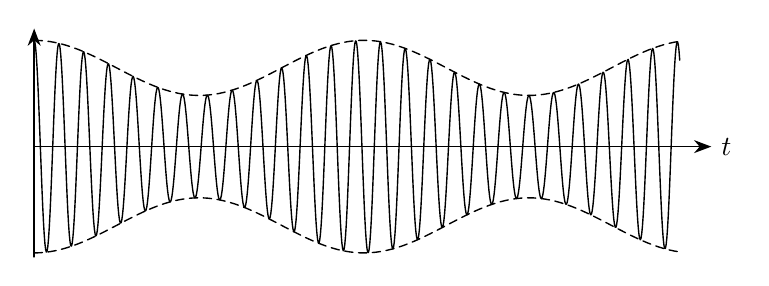
\begin{tikzpicture}[toll,x=1cm,y=1cm]
\draw[tengely] (0,-1.4) -- (0,1.5);\draw[tengely] (0,0) -- (8.6,0) node[right] {$t$};
\draw[szagg,domain=0:8.2,samples=120] plot (\x,{1+0.35*cos(\x*1.5 r)});\draw[szagg,domain=0:8.2,samples=120] plot (\x,{-1-0.35*cos(\x*1.5 r)});
\draw[line width=0.5pt,domain=0:8.2,samples=900] plot (\x,{(1+0.35*cos(\x*1.5 r))*cos(\x*20 r)});
\end{tikzpicture}
\vfill
{\small Az ALL-IN hallgatói gyűjtemény (Moodle-vizsgák 2020, vizsgamegoldások 2014 és 2016 között, témakörös feladatgyűjtemény) alapján, minden eredmény újraszámolva.\par}
\vspace{8mm}
{\small 2026. november\par}
\end{titlepage}
\chapter*{Hogyan használd ezt a könyvet}
Minden feladat ugyanúgy épül fel, hogy vizsgán is ugyanebben a rendben tudj gondolkodni.
\begin{enumerate}
\item \textbf{Feladat.} A feladat szövege, alatta a forrása (vizsga, gyűjtemény, oldal).
\item \textbf{Mit keresünk?} Minden részkérdésnél leírom, melyik mennyiséget keressük, és mit jelent.
\item \textbf{Jelölések ebben a feladatban.} Minden jel jelentése abban a környezetben, ahol épp használjuk, és ha a feladat megadja, az értéke is. Ugyanaz a betű a tárgyban több dolgot is jelenthet (a $k$ lehet Nyquist-zóna sorszáma, felharmonikus sorszáma vagy erősítési tényező), ezért ezt minden feladatnál újra rögzítem.
\item \textbf{Megoldás lépésenként.} Minden matematikai sor alatt kis kapitálissal áll a sor jellege (\textsc{tétel}, \textsc{behelyettesítés}, \textsc{számérték}, \ldots) és egy rövid megjegyzés arról, honnan jön.
\item \textbf{Eredmény}, és szükség esetén \textbf{Figyelem} doboz a tipikus hibákkal, illetve a forrásban talált tévedésekkel (\textbf{Javítás}).
\end{enumerate}

\section*{A színek jelentése}
A könyv fekete-fehér, egyedül a behelyettesítést jelzem színekkel. A feladat által megadott mennyiségek közül legfeljebb ötnek saját színe van: a jelöléstáblában, a képletben a jele, a behelyettesítésnél az értéke ugyanabban a színben jelenik meg. Így ránézésre látszik, mi hova kerül.
\begin{center}
\ca{kék}\quad \cb{narancs}\quad \cc{lila}\quad \cd{kékeszöld}\quad \ce{bíbor}
\end{center}
\behely{\bh{\ca{f_H}}{\ca{75\un{kHz}}}}
\[
f_s\ge2\,\ca{f_H}=2\cdot\ca{75}=150\un{kHz}
\]

\section*{Az ábrákról}
Ahol a feladat rajzot kér, a \textbf{Rajz: ezt kell felrajzolni} doboz pontos ábrát ad, alatta pontokba szedve, hogy kézzel mit kell feltüntetni (tengelyek, jellegzetes értékek, burkoló). Minden ábra papíron egyetlen tollal is megrajzolható.

\section*{Ellenőrzés}
Minden számértéket független szkript számolt újra (\texttt{html/check}). A források hibáit a Javítás doboz és a hibajegyzék (\texttt{03\_Hibajegyzek.md}) rögzíti.

\tableofcontents
\mainmatter
\chapter*{Jelölések jegyzéke}\addcontentsline{toc}{chapter}{Jelölések jegyzéke}\markboth{Jelölések jegyzéke}{}
A tárgyban kevés betűre sok mennyiség jut, ezért ugyanaz a jel a különböző témakörökben mást jelenthet. Az alábbi jegyzék a témakörök alapjelentéseit sorolja fel. Ha egy feladatban más a jelentés, azt a feladat „Jelölések ebben a feladatban” táblázata mondja meg, és az a mérvadó.

{\small\renewcommand{\arraystretch}{1.2}\begin{longtable}{@{}>{\raggedright\arraybackslash}p{2.4cm}>{\raggedright\arraybackslash}p{8.2cm}>{\raggedright\arraybackslash}p{3.8cm}@{}}\toprule
\textbf{Jel} & \textbf{Jelentés} & \textbf{Témakör}\\\midrule\endhead
$a$ & egy kiszolgáló kihasználtsága & Forgalom, VoIP\\
$A$ & a modulátor szorzója & Analóg mod.\\
$A$ & a spektrum értéke 0 Hz-en & PAM, ISI\\
$A$ & felajánlott forgalom & Forgalom, VoIP\\
$A_h$ & hatásos felület & Rádió\\
$A_{h,T}$ & az adóantenna hatásos felülete & Rádió\\
$a_k$ & a k-adik szimbólum amplitúdója & PAM, ISI\\
$a_\mathrm{sz}$ & szakaszcsillapítás & Rádió\\
$\alpha$ & lekerekítési tényező & PAM, ISI\\
$B$ & a jel sávszélessége & Mintavétel\\
$B$ & a generátormátrix paritásrésze & Kódolás\\
$B$ & B paraméter a képletben & Analóg mod.\\
$B$ & a rendelkezésre álló sávszélesség & Digitális mod.\\
$B$ & kék színjel & Hang, látás\\
$B$ & a csatorna sávszélessége & Műsorszórás\\
$B$ & egy hívás sávigénye & Forgalom, VoIP\\
$\mathbf B$ & a generátormátrix paritásrésze & Kódolás\\
$B_\text{be}$ & a bemenő szűrő sávja & Mintavétel\\
$B_\text{ki}$ & a kimenő szűrő sávja & Mintavétel\\
$B_{\min}$ & a legkisebb sávszélesség & Digitális mod.\\
$B_\text{össz}$ & a jel teljes sávszélessége a pozitív frekvenciákon & Mintavétel\\
$B_v$ & a modulált jel sávszélessége & Rádió\\
$\hat c$ & a javított (becsült) kódszó & Kódolás\\
$\hat{\mathbf c}$ & a javított (becsült) kódszó & Kódolás\\
$C$ & csúcstényező: csúcsérték osztva az effektív értékkel & Jelek\\
$C$ & csúcstényező & Mintavétel\\
$\mathcal C$ & a kód, a kódszavak halmaza & Kódolás\\
$C_1$ & az első kód & Kódolás\\
$C_b$ & kék színkülönbségi jel & Hang, látás\\
$c_k$ & a függőleges koordináta & Digitális mod.\\
$C_r$ & vörös színkülönbségi jel & Hang, látás\\
$d$ & átmérő & Rádió\\
$d_k$ & a k-adik szimbólum & PAM, ISI\\
$d_k$ & a vízszintes koordináta & Digitális mod.\\
$d_{\min}$ & kódtávolság, két kódszó legkisebb eltérése & Kódolás\\
$\hat{\mathbf e}$ & a becsült hibavektor & Kódolás\\
$f$ & a bemenő jel frekvenciája & Mintavétel\\
$f$ & vivőfrekvencia & Rádió\\
$f$ & frekvencia & Hang, látás\\
$F$ & a jel frekvenciája & Jelek\\
$F$ & vivőfrekvencia & Analóg mod.\\
$\mathcal F$ & a forrás (forrás ABC) & Kódolás\\
$f_0$ & a 0-s bit frekvenciája & Digitális mod.\\
$f_1$ & a lapos rész vége & PAM, ISI\\
$f_1$ & az 1-es bit frekvenciája & Digitális mod.\\
$f_2$ & ahol a spektrum eléri a nullát & PAM, ISI\\
$f_{AA}$ & a bemenő (antialiasing) szűrő határfrekvenciája & Mintavétel\\
$f_c$ & vivőfrekvencia & Analóg mod.\\
$f_D$ & frekvencialöket & Rádió\\
$f_H$ & a jel legnagyobb frekvenciája & Mintavétel\\
$f_\mathrm{KF}$ & középfrekvencia & Rádió\\
$f_L$ & a jel legkisebb frekvenciája & Mintavétel\\
$f_m$ & a moduláló (mérő)jel frekvenciája & Rádió\\
$f_m$ & a moduláló jel frekvenciája & Analóg mod.\\
$f_\text{osc}$ & az oszcillátor frekvenciája & Rádió\\
$f_R$ & a visszaállító szűrő határfrekvenciája & Mintavétel\\
$f_s$ & mintavételi frekvencia & Mintavétel\\
$f_s$ & mintavételi frekvencia (minta/s) & Kódolás\\
$f_{s,\min}$ & a legkisebb mintavételi frekvencia & Mintavétel\\
$f_t$ & tükörfrekvencia & Rádió\\
$f_v$ & vivőfrekvencia & Analóg mod.\\
$f_v$ & a venni kívánt adó frekvenciája & Műsorszórás\\
$G$ & antennanyereség & Rádió\\
$G$ & generátormátrix & Kódolás\\
$G$ & zöld színjel & Hang, látás\\
$\mathbf G$ & generátormátrix & Kódolás\\
$G_2$ & a második kód generátormátrixa & Kódolás\\
$G_R$ & a vevőantenna nyeresége & Rádió\\
$G_T$ & az adóantenna nyeresége & Rádió\\
$\Gamma$ & a talaj reflexiós tényezője & Rádió\\
$GI$ & a védőintervallum aránya & Műsorszórás\\
$h$ & átlagos tartási idő & Forgalom, VoIP\\
$H$ & a szűrő átvitele & Mintavétel\\
$h_0$ & az elemi jel a saját mintavételi pillanatában & PAM, ISI\\
$h_1$ & az elemi jel egy jelzési idővel később & PAM, ISI\\
$H_\text{be}(f)$ & a bemenő szűrő átvitele & Mintavétel\\
$h_R$ & a vevőantenna magassága & Rádió\\
$h_T$ & az adóantenna magassága & Rádió\\
$H_V$ & a vevőszűrő átvitele & PAM, ISI\\
$H_V(f)$ & a vevőszűrő átvitele & PAM, ISI\\
$H(f)$ & a szűrő átviteli függvénye & Mintavétel\\
$H(f)$ & az elemi jel spektruma & PAM, ISI\\
$H(\mathcal F^2)$ & a szimbólumpárok entrópiája & Kódolás\\
$h(t)$ & elemi jel & PAM, ISI\\
$H^T$ & a paritásellenőrző mátrix transzponáltja & Kódolás\\
$\mathbf H^{\mathsf T}$ & a paritásellenőrző mátrix transzponáltja & Kódolás\\
$I$ & hangintenzitás & Hang, látás\\
$k$ & az üzenet hossza bitben & Kódolás\\
$k$ & erősítési tényező & Digitális mod.\\
$l$ & kódszóhossz & Kódolás\\
$L$ & átlagos kódszóhossz egy szimbólumra & Kódolás\\
$L$ & hangnyomásszint & Hang, látás\\
$\bar L$ & átlagos kódszóhossz & Kódolás\\
$L_1$ & kódszóhossz az első forrásnál & Kódolás\\
$L_1$ & a szint az első helyen & Hang, látás\\
$L_2$ & kódszóhossz a második forrásnál & Kódolás\\
$L_2$ & a szint a második helyen & Hang, látás\\
$l_a$ & az a kódszavának hossza & Kódolás\\
$l_b$ & a b kódszavának hossza & Kódolás\\
$l_c$ & a c kódszavának hossza & Kódolás\\
$l_\text{fej}$ & a fejrészek hossza & Forgalom, VoIP\\
$l_i$ & az i-edik kódszó hossza & Kódolás\\
$L_N$ & hangosságszint (phon) & Hang, látás\\
$l_p$ & egy beszédszegmens hossza & Forgalom, VoIP\\
$L'$ & a vevő bal kimenete & Műsorszórás\\
$L^{(2)}$ & egy szimbólumpár kódszavának hossza & Kódolás\\
$\lambda$ & hullámhossz & Rádió\\
$\lambda$ & hívásintenzitás & Forgalom, VoIP\\
$m$ & modulációs mélység & Analóg mod.\\
$M$ & a konstelláció pontjainak száma & Digitális mod.\\
$M$ & az összegjel (L+R) & Műsorszórás\\
$\mu(t)$ & modulációs tartalom (a fázis eltérése a vivőétől) & Analóg mod.\\
$n$ & a kvantáló bitszáma & Mintavétel\\
$n$ & a kódszó hossza bitben & Kódolás\\
$n$ & szegmensek száma csomagonként & Forgalom, VoIP\\
$N$ & a forrás szimbólumainak száma & Kódolás\\
$N$ & az OFDM-vivők száma & Műsorszórás\\
$N$ & a klaszter cellaszáma (FRF) & GSM\\
$N$ & kiszolgálók száma & Forgalom, VoIP\\
$N_1$ & az első forrás szimbólumainak száma & Kódolás\\
$N_2$ & a második forrás szimbólumainak száma & Kódolás\\
$N_\text{hasznos}$ & az adatot vivő vivők száma & Műsorszórás\\
$n_{\min}$ & a legkisebb kódszóhossz & Kódolás\\
$p$ & egy bit hibavalószínűsége & Kódolás\\
$p$ & hangnyomás & Hang, látás\\
$P$ & átlagteljesítmény 1 $\Omega$-on & Jelek\\
$P$ & a jel teljesítménye & Mintavétel\\
$P$ & átlagteljesítmény & Analóg mod.\\
$P$ & elektromos teljesítmény & Hang, látás\\
$p_0$ & a hallásküszöb hangnyomása & Hang, látás\\
$p_1$ & a keresett hangnyomás & Hang, látás\\
$p_a$ & az a szimbólum valószínűsége & Kódolás\\
$p_A$ & az A szimbólum valószínűsége & Kódolás\\
$P_a$ & az a) elrendezés átlagteljesítménye & Digitális mod.\\
$p_b$ & a b szimbólum valószínűsége & Kódolás\\
$p_B$ & a B szimbólum valószínűsége & Kódolás\\
$P_b$ & a b) elrendezés átlagteljesítménye & Digitális mod.\\
$P_b$ & blokkolási valószínűség & Forgalom, VoIP\\
$p_C$ & a C szimbólum valószínűsége & Kódolás\\
$P_c$ & a c) elrendezés átlagteljesítménye & Digitális mod.\\
$P_R$ & vett teljesítmény & Rádió\\
$P_{R,\min}$ & a vevő érzékenysége (a legkisebb vehető teljesítmény) & Rádió\\
$P_T$ & adóteljesítmény & Rádió\\
$p(0)$ & a 0 szint valószínűsége & Kódolás\\
$P(0)$ & annak valószínűsége, hogy egy bit sem hibás & Kódolás\\
$P(1)$ & annak valószínűsége, hogy pontosan 1 bit hibás & Kódolás\\
$P(2)$ & annak valószínűsége, hogy pontosan 2 bit hibás & Kódolás\\
$p(\pm1)$ & a $\pm$1 szint valószínűsége & Kódolás\\
$p(\pm2)$ & a $\pm$2 szint valószínűsége & Kódolás\\
$p(\pm3)$ & a $\pm$3 szint valószínűsége & Kódolás\\
$\Phi_D$ & fázislöket & Analóg mod.\\
$r$ & az adó és a vevő távolsága & Rádió\\
$r$ & szimbólumsebesség (szimbólum/s) & Kódolás\\
$R$ & az ellenállás & Mintavétel\\
$R$ & a parabola sugara & Rádió\\
$R$ & terhelő ellenállás & Analóg mod.\\
$R$ & vörös színjel & Hang, látás\\
$r_0$ & a zónahatár távolsága & Rádió\\
$r_1$ & az első távolság & Hang, látás\\
$r_2$ & a második távolság & Hang, látás\\
$r_{\max}$ & a legnagyobb távolság & Rádió\\
$R_s$ & szimbólumsebesség & Digitális mod.\\
$R'$ & a vevő jobb kimenete & Műsorszórás\\
$RC$ & a burkolódemodulátor időállandója & Analóg mod.\\
$s$ & szindróma & Kódolás\\
$\hat s$ & a modulált jel csúcsértéke & Analóg mod.\\
$S$ & a különbségi (L$-$R) jel & Műsorszórás\\
$s_0$ & a teljesítménysűrűség & Mintavétel\\
$s_\mathrm{FM}(t)$ & az FM-jel & Analóg mod.\\
$s_m(t)$ & a moduláló jel & Analóg mod.\\
$s(t)$ & a modulált jel & Analóg mod.\\
$\text{SNR}$ & jel-zaj viszony & Jelek\\
$\Delta\text{SNR}$ & a jel-zaj viszony változása & Jelek\\
$T$ & mintavételi idő & Mintavétel\\
$T$ & jelzési idő & PAM, ISI\\
$T$ & jelzési (bit-) idő & Digitális mod.\\
$t_0$ & a mintavétel helye a jelzési időn belül & PAM, ISI\\
$T_0$ & a moduláló jel félperiódusa & Analóg mod.\\
$T_0$ & a mintavétel helye a jelzési időn belül & PAM, ISI\\
$T_0$ & hasznos szimbólumidő & Műsorszórás\\
$T_1$ & első mintavételi idő & Mintavétel\\
$T_2$ & második mintavételi idő & Mintavétel\\
$T_m$ & a moduláló jel periódusideje & Analóg mod.\\
$\hat u$ & a becsült üzenet & Kódolás\\
$\hat{\mathbf u}$ & a becsült üzenet & Kódolás\\
$U$ & a bemenő jel amplitúdója & Mintavétel\\
$U$ & a modulált jel amplitúdója & Analóg mod.\\
$U$ & a jel amplitúdója & Digitális mod.\\
$U_0$ & egyenszint (a burkoló középértéke) & Analóg mod.\\
$U_{6{,}2}$ & a kimenő 6,2 kHz-es összetevő amplitúdója & Mintavétel\\
$U_m$ & a burkoló kilengése & Analóg mod.\\
$v$ & a vett szó & Kódolás\\
$v$ & bitsebesség & PAM, ISI\\
$\mathbf v$ & a vett szó & Kódolás\\
$v_\text{cs}$ & csomagsebesség & Forgalom, VoIP\\
$v_\text{forrás}$ & a kodek bitsebessége & Forgalom, VoIP\\
$v_\text{nettó}$ & nettó bitsebesség & Műsorszórás\\
$V(\lambda)$ & láthatósági függvény & Hang, látás\\
$\varphi$ & fázishiba & Digitális mod.\\
$\varphi_{\max}$ & a megengedett fázishiba & Digitális mod.\\
$\hat x$ & csúcsérték, a jel legnagyobb abszolút értéke & Jelek\\
$\hat x$ & a jel csúcsértéke & Analóg mod.\\
$x(t)$ & a vizsgált jel & Jelek\\
$x(t)$ & a moduláló jel & Analóg mod.\\
$x(t)$ & a PAM-jel & PAM, ISI\\
$Y$ & világossági jel & Hang, látás\\
\bottomrule\end{longtable}}
% Generálva: html/build_tex.js (ai01.js). Kézzel ne szerkeszd, a forrás a html/data mappa.
\setcounter{chapter}{0}
\chapter{\texorpdfstring{Jelek, teljesítmény, csúcstényező}{Jelek, teljesítmény, csúcstényező}}\label{f1}
Rövid, de a vizsgán gyakori kérdések: mekkora egy összetett jel csúcsértéke, teljesítménye és csúcstényezője. A kulcs: azonos frekvenciájú összetevők egyetlen szinusszá adódnak össze, különböző frekvenciájúak nem.

\section{Alapok, egyszerűen}
\subsection{\texorpdfstring{A1. Jelölések: teljesítmény és csúcstényező}{A1. Jelölések: teljesítmény és csúcstényező}}\label{a1-teljesitmeny}
\par\noindent{\small\renewcommand{\arraystretch}{1.25}\begin{tabularx}{\linewidth}{@{}>{\raggedright\arraybackslash}X>{\raggedright\arraybackslash}X@{}}\toprule
\textbf{Jel} & \textbf{Jelentés}\\\midrule
undefined & csúcsérték: a jel legnagyobb abszolút értéke\\
undefined & átlagteljesítmény 1 $\Omega$-on: a jel négyzetének időátlaga, undefined\\
undefined & effektív érték, undefined\\
undefined & csúcstényező, undefined\\
\bottomrule\end{tabularx}}\par

Egy $A$ amplitúdójú szinusz teljesítménye $A^2/2$, mert $\sin^2$ átlaga egy perióduson $1/2$. Ezért szinuszra $C=A/(A/\sqrt2)=\sqrt2$. Négyszögjelre $C=1$, háromszögjelre $\sqrt3$.

Különböző frekvenciájú szinuszok szorzatának átlaga 0, ezért a teljesítményük \textbf{összeadódik}: $P=\sum A_i^2/2$. Ugyanez igaz egy azonos frekvenciájú $\sin$ és $\cos$ párra is.

\subsection{\texorpdfstring{A2. Azonos frekvenciájú összetevők összeadása}{A2. Azonos frekvenciájú összetevők összeadása}}\label{a1-fazor}
Az addíciós tétellel $A\sin(\omega t+\varphi)=A\cos\varphi\sin\omega t+A\sin\varphi\cos\omega t$. Összevetve az $a\sin\omega t+b\cos\omega t$ alakkal: $A\cos\varphi=a$, $A\sin\varphi=b$, ezért

\begin{center}\adjustbox{max width=\linewidth}{$\displaystyle a\sin\omega t+b\cos\omega t=\sqrt{a^2+b^2}\,\sin(\omega t+\varphi),\qquad\mathrm{tg}\,\varphi=\frac ba$}\end{center}

Gondolj két egymásra merőleges nyílra: az eredő hossza Pitagorasz-tétellel jön ki. A csúcsérték ezért nem $a+b$, hanem $\sqrt{a^2+b^2}$.

Ha a frekvenciák aránya irracionális (pl. $\sqrt2$), a két szinusz előbb-utóbb tetszőlegesen közel kerül egyszerre a csúcsához, ezért a csúcsérték az amplitúdók \textbf{összege}.

% ------------------------------------------------------------------
\section{\texorpdfstring{1.1. feladat: $3\sin+4\cos$: csúcsérték, teljesítmény, csúcstényező}{1.1. feladat: 3sin+4cos: csúcsérték, teljesítmény, csúcstényező}}\label{ai1_01}
\setcounter{lepes}{0}
\begin{feladat}{1.1. feladat}
Határozza meg az $x(t)=3\sin(2\pi Ft)+4\cos(2\pi Ft)$ jel csúcstényezőjét, maximális értékét és teljesítményét!

{\footnotesize\sffamily Forrás: ALL-IN 90. oldal $\cdot$ aiD\_1\_1 (és 5-ösöm 2. oldal). Címkék: beugró, javítás}
\end{feladat}
\begin{keresunk}
\begin{itemize}
\item $C$: csúcstényező
\item $\hat x$: legnagyobb érték
\item $P$: átlagteljesítmény (1 $\Omega$-on)
\end{itemize}
\end{keresunk}
\begin{jeloles}
\begin{jeltabla}
$F$ & a jel frekvenciája & \\
$C$ & csúcstényező: csúcsérték osztva az effektív értékkel & \emph{keresett}\\
$\hat x$ & csúcsérték, a jel legnagyobb abszolút értéke & \emph{keresett}\\
$P$ & átlagteljesítmény 1 $\Omega$-on & \emph{keresett}\\
$a$ & a szinuszos tag együtthatója (3) & \\
$\omega$ & körfrekvencia, a frekvencia 2$\pi$-szerese & \\
$b$ & a koszinuszos tag együtthatója (4) & \\
$\varphi$ & az összevont szinusz kezdőfázisa & \\
$A$ & az összevont szinusz amplitúdója, 5 & \\
$x_\text{eff}$ & a jel effektív értéke & \\
\end{jeltabla}
\par\smallskip\textbf{Adott még:}
\begin{itemize}
\item $x(t)$: két azonos, $F$ frekvenciájú tag, a szinuszos amplitúdója 3, a koszinuszosé 4
\item $F$: a két tag közös frekvenciája. Az értéke nem kell, az eredmény nem függ tőle
\end{itemize}
\end{jeloles}
\begin{elmelet}[Miért így? Egyszerűen]
\textbf{Miért nem $3+4=7$ a csúcs?}\par Mert a szinusz és a koszinusz negyed periódussal el van tolva, soha nem érik el egyszerre a csúcsukat. Az eredő egyetlen szinusz (A2).
\end{elmelet}

\lepes{Egyetlen szinusszá alakítás}
Az $a\sin\omega t+b\cos\omega t=\sqrt{a^2+b^2}\,\sin(\omega t+\varphi)$ összevonással, ahol $a=3$, $b=4$ és $\omega=2\pi F$.

\begin{center}\adjustbox{max width=\linewidth}{$\displaystyle A=\sqrt{a^2+b^2}=\sqrt{3^2+4^2}=\sqrt{25}=5$}\end{center}
\jegyzet{tétel}{}

\begin{center}\adjustbox{max width=\linewidth}{$\displaystyle \mathrm{tg}\,\varphi=\tfrac43\ \Rightarrow\ \varphi=53{,}1^{\circ}$}\end{center}
\jegyzet{számérték}{$x(t)=5\sin(\omega t+53{,}1^{\circ})$}

\lepes{A maximális érték}
A szinusz legnagyobb értéke 1, ezért a jelé az amplitúdó.

\begin{center}\adjustbox{max width=\linewidth}{$\displaystyle \hat x=5$}\end{center}
\jegyzet{számérték}{}

\lepes{A teljesítmény}
A $\sin$ és a $\cos$ szorzatának átlaga 0, ezért a két tag teljesítménye összeadódik (A1). Ugyanez jön ki az összevont szinuszból is.

\begin{center}\adjustbox{max width=\linewidth}{$\displaystyle P=\frac{3^2}{2}+\frac{4^2}{2}=4{,}5+8=12{,}5\ \text{W}$}\end{center}
\jegyzet{definíció}{1 $\Omega$-on}

\begin{center}\adjustbox{max width=\linewidth}{$\displaystyle \frac{5^2}{2}=12{,}5$}\end{center}
\jegyzet{ellenőrzés}{egyezik}

\lepes{A csúcstényező}


\begin{center}\adjustbox{max width=\linewidth}{$\displaystyle x_\text{eff}=\sqrt{12{,}5}=3{,}54\qquad C=\frac{\hat x}{x_\text{eff}}=\frac{5}{3{,}54}=\sqrt2$}\end{center}
\jegyzet{definíció}{mint minden szinuszé}
\begin{tipp}[A gyűjtemény megoldása]
A csúcstényezőt ($\sqrt2$) és a teljesítményt jól adja, a maximumot viszont ott keresi, ahol $\sin=\cos$, és $7/\sqrt2\approx4{,}95$-öt kap.
\end{tipp}
\begin{figyelem}[Javítás]
A maximum nem a $\sin=\cos$ (45\textdegree{}-os) pontban van, hanem $\varphi=53{,}1^{\circ}$-nál. Helyesen $\hat x=5$.
\end{figyelem}
\begin{eredmeny}

\begin{center}\adjustbox{max width=\linewidth}{$\displaystyle C=\sqrt2\qquad\hat x=5\qquad P=12{,}5\ \text{W (1 }\Omega\text{-on)}$}\end{center}
\end{eredmeny}
\begin{figyelem}[Tipikus hibák]
\begin{itemize}
\item A két amplitúdó összeadása ($7$), vagy egy önkényesen választott időpontban vett érték.
\end{itemize}
\end{figyelem}


% ------------------------------------------------------------------
\section{\texorpdfstring{1.2. feladat: Két koszinusz, $f_1/f_2=\sqrt2$}{1.2. feladat: Két koszinusz, f1/f2=√2}}\label{ai1_02}
\setcounter{lepes}{0}
\begin{feladat}{1.2. feladat}
Mekkora az $x(t)=2\cos(2\pi f_1t)+2\cos(2\pi f_2t)$ jel csúcstényezője, legnagyobb értéke és teljesítménye, ha $f_1/f_2=\sqrt2$?

{\footnotesize\sffamily Forrás: ALL-IN 90. oldal $\cdot$ aiD\_1\_2. Címkék: beugró}
\end{feladat}
\begin{keresunk}
\begin{itemize}
\item $C$ (csúcstényező: csúcsérték osztva az effektív értékkel), $\hat x$ (csúcsérték, a jel legnagyobb abszolút értéke), $P$ (átlagteljesítmény 1 $\Omega$-on)
\end{itemize}
\end{keresunk}
\begin{jeloles}
\begin{jeltabla}
$f_1$ & az első koszinusz frekvenciája & \\
$f_2$ & a második koszinusz frekvenciája & \\
$C$ & csúcstényező: csúcsérték osztva az effektív értékkel & \emph{keresett}\\
$\hat x$ & csúcsérték, a jel legnagyobb abszolút értéke & \emph{keresett}\\
$P$ & átlagteljesítmény 1 $\Omega$-on & \emph{keresett}\\
$x$ & a vizsgált jel, x(t) & \\
\end{jeltabla}
\par\smallskip\textbf{Adott még:}
\begin{itemize}
\item két koszinusz, mindkettő 2 amplitúdójú
\end{itemize}
\end{jeloles}
\begin{elmelet}[Miért így? Egyszerűen]
\textbf{Miért $4$ a csúcs?}\par Az irracionális frekvenciaarány miatt a két fázis „mindenféle” párosítást bejár, köztük tetszőlegesen közel kerülnek a $(0,0)$ fázispárhoz, ahol mindkét koszinusz 1 (A2).
\end{elmelet}

\lepes{A legnagyobb érték}
Egyik tag sem lehet 2-nél nagyobb, és a két csúcs tetszőlegesen közel kerül egymáshoz.

\begin{center}\adjustbox{max width=\linewidth}{$\displaystyle \hat x=2+2=4$}\end{center}
\jegyzet{közelítés}{tetszőlegesen megközelíthető}

\lepes{A teljesítmény}
Különböző frekvenciák, a teljesítmények összeadódnak (A1).

\begin{center}\adjustbox{max width=\linewidth}{$\displaystyle P=\frac{2^2}{2}+\frac{2^2}{2}=2+2=4$}\end{center}
\jegyzet{definíció}{}

\lepes{A csúcstényező}


\begin{center}\adjustbox{max width=\linewidth}{$\displaystyle C=\frac{\hat x}{\sqrt P}=\frac{4}{\sqrt4}=2$}\end{center}
\jegyzet{definíció}{}
\begin{eredmeny}

\begin{center}\adjustbox{max width=\linewidth}{$\displaystyle \hat x=4\qquad P=4\ (\text{W, }1\,\Omega)\qquad C=2$}\end{center}
\end{eredmeny}
\begin{tipp}[Ellenőrzés]
\begin{itemize}
\item A gyűjtemény is 2, 4, 4 értéket ad. Ha a frekvenciák egyformák lennének, $x=4\cos$, $C=\sqrt2$ jönne ki: a különbség az összemérhetetlenségből adódik.
\end{itemize}
\end{tipp}


% ------------------------------------------------------------------
\section{\texorpdfstring{1.3. feladat: $4\sin-3\cos$: négy állítás}{1.3. feladat: 4sin-3cos: négy állítás}}\label{ai1_03}
\setcounter{lepes}{0}
\begin{feladat}{1.3. feladat}
Az $s(t)=4\sin(2\pi f_0t)-3\cos(2\pi f_0t)$ jel: A) csúcsértéke 4. B) csúcstényezője $1/\sqrt2$. C) $t=42/f_0$-ban az értéke $-4$. D) átlagteljesítménye 3,5. Melyik igaz?

{\footnotesize\sffamily Forrás: ALL-IN 91. oldal $\cdot$ aiD\_1\_3 (feleletválasztós 4.6.). Címkék: beugró, javítás}
\end{feladat}
\begin{keresunk}
\begin{itemize}
\item melyik állítás igaz
\end{itemize}
\end{keresunk}
\begin{jeloles}
\begin{jeltabla}
$s$ & a vizsgált jel, s(t) & \\
$f_0$ & a két tag közös frekvenciája & \\
$a$ & a szinuszos tag együtthatója (4) & \\
$\omega$ & körfrekvencia, a frekvencia 2$\pi$-szerese & \\
$b$ & a koszinuszos tag együtthatója ($-$3) & \\
$\varphi$ & az összevont szinusz kezdőfázisa & \\
$\hat s$ & a jel csúcsértéke & \\
$C$ & csúcstényező: csúcsérték osztva az effektív értékkel & \\
$P$ & átlagteljesítmény 1 $\Omega$-on & \\
\end{jeltabla}
\par\smallskip\textbf{Adott még:}
\begin{itemize}
\item azonos frekvenciájú szinusz (4) és koszinusz ($-3$)
\end{itemize}
\end{jeloles}

\lepes{A) csúcsérték}
Az $a\sin\omega t+b\cos\omega t=\sqrt{a^2+b^2}\,\sin(\omega t+\varphi)$ összevonással, ahol $a=4$, $b=-3$.

\begin{center}\adjustbox{max width=\linewidth}{$\displaystyle \hat s=\sqrt{4^2+(-3)^2}=5$}\end{center}
\jegyzet{tétel}{A hamis}

\lepes{B) csúcstényező}
Az összeg egyetlen szinusz, ezért $C=\sqrt2$. Az $1/\sqrt2$ már csak azért is rossz, mert $C\ge1$ mindig.

\begin{center}\adjustbox{max width=\linewidth}{$\displaystyle C=\frac{5}{5/\sqrt2}=\sqrt2$}\end{center}
\jegyzet{számérték}{B hamis}

\lepes{C) A jel értéke a $t=42/f_0$ időpontban}
Behelyettesítve az argumentum $2\pi\cdot42$, ez egész számú periódus.

\begin{center}\adjustbox{max width=\linewidth}{$\displaystyle s=4\sin(84\pi)-3\cos(84\pi)=4\cdot0-3\cdot1=-3$}\end{center}
\jegyzet{behelyettesítés}{C hamis}

\lepes{D) átlagteljesítmény}


\begin{center}\adjustbox{max width=\linewidth}{$\displaystyle P=\frac{4^2}{2}+\frac{3^2}{2}=8+4{,}5=12{,}5$}\end{center}
\jegyzet{definíció}{D hamis}
\begin{figyelem}[Javítás]
A gyűjtemény lapján A, B, C be van karikázva. Ha ez a „hamis” jelölése, a megoldás helyes, igaznak jelölve mindhárom rossz.
\end{figyelem}
\begin{eredmeny}

\begin{center}\adjustbox{max width=\linewidth}{$\displaystyle \text{egyik állítás sem igaz}$}\end{center}
\end{eredmeny}


% ------------------------------------------------------------------
\section{\texorpdfstring{1.4. feladat: $2\sin+2\cos$ csúcstényezője}{1.4. feladat: 2sin+2cos csúcstényezője}}\label{ai1_04}
\setcounter{lepes}{0}
\begin{feladat}{1.4. feladat}
Határozza meg az $x(t)=2\sin(2\pi ft)+2\cos(2\pi ft)$ jel csúcstényezőjét!

{\footnotesize\sffamily Forrás: ALL-IN 91. oldal $\cdot$ aiD\_1\_5. Címkék: beugró}
\end{feladat}
\begin{keresunk}
\begin{itemize}
\item $C$ (csúcstényező: csúcsérték osztva az effektív értékkel)
\end{itemize}
\end{keresunk}
\begin{jeloles}
\begin{jeltabla}
$C$ & csúcstényező: csúcsérték osztva az effektív értékkel & \emph{keresett}\\
$x$ & a vizsgált jel, x(t) & \\
$f$ & a két tag közös frekvenciája & \\
$a$ & a szinuszos tag együtthatója (2) & \\
$\omega$ & körfrekvencia, a frekvencia 2$\pi$-szerese & \\
$b$ & a koszinuszos tag együtthatója (2) & \\
$\varphi$ & az összevont szinusz kezdőfázisa & \\
$A$ & az összevont szinusz amplitúdója, $2\sqrt2$ & \\
$\hat x$ & csúcsérték, a jel legnagyobb abszolút értéke & \\
$P$ & átlagteljesítmény 1 $\Omega$-on & \\
\end{jeltabla}
\par\smallskip\textbf{Adott még:}
\begin{itemize}
\item azonos frekvenciájú szinusz és koszinusz, mindkettő 2 amplitúdójú
\end{itemize}
\end{jeloles}

\lepes{Egyetlen szinusz}
Az $a\sin\omega t+b\cos\omega t=\sqrt{a^2+b^2}\,\sin(\omega t+\varphi)$ összevonással, ahol $a=b=2$.

\begin{center}\adjustbox{max width=\linewidth}{$\displaystyle A=\sqrt{2^2+2^2}=2\sqrt2\qquad\mathrm{tg}\,\varphi=1\ \Rightarrow\ \varphi=45^{\circ}$}\end{center}
\jegyzet{tétel}{$x=2\sqrt2\sin(2\pi ft+45^{\circ})$}

\lepes{Csúcstényező}
Szinuszos jel, $\hat x=2\sqrt2$, $P=(2\sqrt2)^2/2=4$.

\begin{center}\adjustbox{max width=\linewidth}{$\displaystyle C=\frac{2\sqrt2}{\sqrt4}=\sqrt2$}\end{center}
\jegyzet{definíció}{}
\begin{eredmeny}

\begin{center}\adjustbox{max width=\linewidth}{$\displaystyle C=\sqrt2\qquad(\hat x=2\sqrt2,\ P=4)$}\end{center}
\end{eredmeny}

% Generálva: html/build_tex.js (ai02.js). Kézzel ne szerkeszd, a forrás a html/data mappa.
\setcounter{chapter}{1}
\chapter{\texorpdfstring{Mintavételezés és kvantálás}{Mintavételezés és kvantálás}}\label{f2}
A gyűjtemény leggyakoribb feladattípusa. Három kérdés ismétlődik: milyen $f_s$ mellett állítható vissza a jel, milyen frekvenciájú és mekkora komponensek jelennek meg a kimeneten, és hány bit kell egy adott jel-zaj viszonyhoz.

\section{Alapok, egyszerűen}
\subsection{\texorpdfstring{A1. Jelölések, álképek, két szűrő}{A1. Jelölések, álképek, két szűrő}}\label{a2-tetel}
\par\noindent{\small\renewcommand{\arraystretch}{1.25}\begin{tabularx}{\linewidth}{@{}>{\raggedright\arraybackslash}X>{\raggedright\arraybackslash}X@{}}\toprule
\textbf{Jel} & \textbf{Jelentés}\\\midrule
undefined & mintavételi frekvencia (undefined a mintavételi idő)\\
undefined & a jel legkisebb és legnagyobb frekvenciája, undefined a sávszélessége\\
undefined & az elő- (antialiasing) és az utó- (visszaállító) szűrő átvitele\\
undefined & a kvantáló bitszáma\\
undefined & a jel csúcstényezője\\
\bottomrule\end{tabularx}}\par

A mintavétel a spektrumot $f_s$-enként megismétli, ezért egy $f$ frekvenciájú bemenet után $nf_s\pm f$ helyeken jelennek meg vonalak. Az \textbf{előszűrő} a mintavétel előtt az eredeti frekvencián csillapít (az átlapolódás ellen), az \textbf{utószűrő} a D/A után az új frekvencián (a „szivárgás” ellen). Egy komponens kimeneti amplitúdója:

\begin{center}\adjustbox{max width=\linewidth}{$\displaystyle U_\text{ki}=U_\text{be}\cdot H_\text{elő}(f_\text{be})\cdot H_\text{utó}(f_\text{ki})$}\end{center}

40 dB csillapítás feszültségben 0,01-es szorzó ($20\lg0{,}01=-40$). Alapsávi jelnél a tétel: $f_s>2f_{\max}$ (szigorúan, a határeset szinusznál nem működik).

\subsection{\texorpdfstring{A2. Sáváteresztő jel mintavételezése}{A2. Sáváteresztő jel mintavételezése}}\label{a2-sav}
Ha a jel csak $f_L\ldots f_H$ között van, elég, ha a másolatok a sávok közötti résbe esnek. A megengedett tartományok egész $k$-ra:

\begin{center}\adjustbox{max width=\linewidth}{$\displaystyle \frac{2f_H}{k}\le f_s\le\frac{2f_L}{k-1}\qquad k=1,2,\ldots,\lfloor f_H/B\rfloor$}\end{center}

$k=1$ a szokásos $f_s\ge2f_H$ (a felső határ végtelen). Nagyobb $k$-nál a visszaállításhoz \textbf{sávszűrő} kell. A legnagyobb $k$-nál túl a tartomány alsó határa nagyobb lenne a felsőnél, ott nincs megoldás.

\subsection{\texorpdfstring{A3. Kvantálási jel-zaj viszony}{A3. Kvantálási jel-zaj viszony}}\label{a2-snr}
\begin{center}\adjustbox{max width=\linewidth}{$\displaystyle \frac SN=\frac{3}{C^2}\cdot\frac{f_s}{2B_z}\cdot2^{2n}\qquad \left(\frac SN\right)_\mathrm{dB}=10\lg\frac3{C^2}+10\lg\frac{f_s}{2B_z}+6{,}02\,n$}\end{center}

$B_z$ a visszaállító szűrő sávja: a kvantálási zaj a $0\ldots f_s/2$ tartományban terül szét egyenletesen, és ennek csak a szűrőn átjutó része marad meg. Szinusz ($C=\sqrt2$): $1{,}76+6{,}02n$ dB. Háromszög ($C=\sqrt3$): $6{,}02n$ dB. A jel-zaj viszony \textbf{teljesítményarány}, ezért 60 dB $=10^6$, nem $10^3$. A bitszámot felfelé kerekítjük.

% ------------------------------------------------------------------
\section{\texorpdfstring{2.1. feladat: Mi jelenik meg a kimeneten? 8 kHz, 40 dB-es szűrők}{2.1. feladat: Mi jelenik meg a kimeneten? 8 kHz, 40 dB-es szűrők}}\label{ai2_01}
\setcounter{lepes}{0}
\begin{feladat}{2.1. feladat}
Egy $8$ kHz-es digitális rendszer a 2 V-os 1,5 kHz-es jelet amplitúdóhelyesen továbbítja. Az elő- és a visszaállító szűrő 4 kHz sávhatárú aluláteresztő, a zárótartományban 40 dB csillapítással. a) Mi jelenik meg a kimeneten 3,5 kHz-es, 2 V-os bemenetre? b) Milyen 2 mV-nál nagyobb komponensek várhatók, ha a bemenet 1, 3 és 5 kHz-es, egyenként 2 V-os? c) Mi változik b)-hez képest 1,5 és 3 kHz-es bemenetnél, ha az előszűrőt elhagyjuk?

{\footnotesize\sffamily Forrás: ALL-IN 92\ldots{}93. oldal $\cdot$ aiD\_2\_1. Címkék: vizsga}
\end{feladat}
\begin{keresunk}
\begin{itemize}
\item a), b), c) a kimenő összetevők frekvenciája és amplitúdója
\end{itemize}
\end{keresunk}
\begin{jeloles}
\begin{jeltabla}
$\ca{f_s}$ & mintavételi frekvencia & $8$\,kHz\\
$\cb{H}$ & a szűrő átvitele & $1$\\
$n$ & tetszőleges egész szám (hányadik mintavételi többszörös) & \\
$f$ & egy kimenő összetevő frekvenciája & \\
$U_{3{,}5}$ & a kimenő 3,5 kHz-es összetevő amplitúdója & \\
$U_{4{,}5}$ & a kimenő 4,5 kHz-es összetevő amplitúdója & \\
$U_{11{,}5}$ & a kimenő 11,5 kHz-es összetevő amplitúdója & \\
$U_5$ & az 5 kHz-es összetevő amplitúdója a mintavevő bemenetén & \\
$U_{3\,\text{kHz}}$ & a kimenő 3 kHz-es összetevő amplitúdója & \\
\end{jeltabla}
\end{jeloles}
\begin{elmelet}[Miért így? Egyszerűen]
\textbf{Miért 20 mV minden „kép”?}\par A 40 dB feszültségben 100-szoros csillapítás: $2\ \text{V}/100=20$ mV. Ami egyszer a zárótartományba esik, ennyi lesz, ami kétszer, $0{,}2$ mV.
\end{elmelet}

\lepes{a) 3,5 kHz}
A 3,5 kHz a sávban van, az előszűrő átengedi. Mintavétel után vonalak $n\cdot8\pm3{,}5$ kHz-en (A1). Az utószűrő a 4 kHz felettieket 0,01-szeresre csillapítja.

\begin{center}\adjustbox{max width=\linewidth}{$\displaystyle f\in\{3{,}5;\ 4{,}5;\ 11{,}5;\ 12{,}5;\ 19{,}5;\ \ldots\}\ \text{kHz}$}\end{center}
\jegyzet{definíció}{$8\pm3{,}5$, $16\pm3{,}5$, \ldots{}}

\begin{center}\adjustbox{max width=\linewidth}{$\displaystyle U_{3{,}5}=2\ \text{V}\qquad U_{4{,}5}=U_{11{,}5}=\ldots=2\cdot0{,}01=20\ \text{mV}$}\end{center}
\jegyzet{számérték}{}

\lepes{b) Az előszűrő után}
Az 1 és a 3 kHz átjut (2 V), az 5 kHz a zárótartományban van.

\begin{center}\adjustbox{max width=\linewidth}{$\displaystyle U_5=2\cdot0{,}01=20\ \text{mV}$}\end{center}
\jegyzet{számérték}{az 5 kHz a mintavevőn}

\lepes{b) Mintavétel és utószűrő}
Az 5 kHz-es (20 mV-os) összetevő álképe $8-5=3$ kHz, a sávba esik, és összeadódik a valódi 3 kHz-cel. Az 1 és 3 kHz álképei ($n\cdot8\pm1$, $n\cdot8\pm3$) 4 kHz felett vannak, 0,01-szeresre csillapodnak.

\begin{center}\adjustbox{max width=\linewidth}{$\displaystyle U_{3\,\text{kHz}}=2\ \text{V}\pm20\ \text{mV}$}\end{center}
\jegyzet{számérték}{a fázistól függően}

\begin{center}\adjustbox{max width=\linewidth}{$\displaystyle 5,\ 7,\ 9,\ 11,\ 13,\ 15,\ \ldots\ \text{kHz: }2\cdot0{,}01=20\ \text{mV}$}\end{center}
\jegyzet{definíció}{$8-3$, $8-1$, $8+1$, $8+3$, $16-3$, \ldots{}}

\begin{center}\adjustbox{max width=\linewidth}{$\displaystyle \text{az 5 kHz saját vonala: }2\cdot0{,}01\cdot0{,}01=0{,}2\ \text{mV}<2\ \text{mV}$}\end{center}
\jegyzet{ellenőrzés}{kétszer csillapodik, elhanyagolható}

\lepes{c) Előszűrő nélkül}
Az 1,5 és a 3 kHz is 4 kHz alatt van, az előszűrő úgysem csillapította őket. Átlapolódás csak 4 kHz feletti bemenetből lehetne, ilyen nincs: semmi sem változik.

\begin{center}\adjustbox{max width=\linewidth}{$\displaystyle 1{,}5\ \text{és}\ 3\ \text{kHz: }2\ \text{V}\qquad n\cdot8\pm1{,}5,\ n\cdot8\pm3\ \text{kHz: }20\ \text{mV}$}\end{center}
\jegyzet{számérték}{}
\begin{tipp}[A gyűjtemény megoldása]
A hallgatói kézírás ugyanezt adja, a 3 kHz-re „2,02 V”-ot írva.
\end{tipp}
\begin{eredmeny}

\begin{center}\adjustbox{max width=\linewidth}{$\displaystyle \text{a) }3{,}5\ \text{kHz }2\ \text{V},\ n\cdot8\pm3{,}5\ \text{kHz }20\ \text{mV}\qquad\text{b) }1\ \text{kHz }2\ \text{V},\ 3\ \text{kHz }2\ \text{V}\pm20\ \text{mV},\ \text{a képek }20\ \text{mV}\qquad\text{c) nem változik}$}\end{center}
\end{eredmeny}
\begin{figyelem}[Tipikus hibák]
\begin{itemize}
\item Az 5 kHz-en mért 20 mV-ot az 5 kHz-es bemenetnek tulajdonítani. Az valójában a 3 kHz képe ($8-3$).
\end{itemize}
\end{figyelem}


% ------------------------------------------------------------------
\section{\texorpdfstring{2.2. feladat: 45\ldots{}75 kHz-es jel mintavételezése}{2.2. feladat: 45…75 kHz-es jel mintavételezése}}\label{ai2_02}
\setcounter{lepes}{0}
\begin{feladat}{2.2. feladat}
Egy jelnek 45 és 75 kHz között vannak komponensei, közvetlenül digitalizáljuk. a) Mekkora $f_s$ kell aluláteresztővel? b) Sávszűrővel? c) Rajzolja fel a spektrumot a legkisebb $f_s$-sel!

{\footnotesize\sffamily Forrás: ALL-IN 18. oldal $\cdot$ ai2016\_01\_05\_1. Címkék: vizsga, javítás}
\end{feladat}
\begin{keresunk}
\begin{itemize}
\item a) $f_s$ (mintavételi frekvencia) aluláteresztő visszaállításhoz
\item b) $f_s$ (mintavételi frekvencia) sávszűrős visszaállításhoz
\item c) a spektrum $f_{s,\min}$-nél (a legkisebb mintavételi frekvencia)
\end{itemize}
\end{keresunk}
\begin{jeloles}
\begin{jeltabla}
$\ca{f_L}$ & a jel legkisebb frekvenciája & $45$\,kHz\\
$\cb{f_H}$ & a jel legnagyobb frekvenciája & $75$\,kHz\\
$f_s$ & mintavételi frekvencia & \emph{keresett}\\
$f_{s,\min}$ & a legkisebb mintavételi frekvencia & \emph{keresett}\\
$k$ & a Nyquist-zóna sorszáma: a frekvenciatengelyt $f_s/2$ széles sávokra osztjuk, és $k$ annak a sávnak a sorszáma, amelybe a jel teljes sávja beleesik & \\
$B$ & a jel sávszélessége & \\
$k_{\max}$ & a legnagyobb szóba jöhető zónasorszám, $\lfloor f_H/B\rfloor$ & \\
$n$ & a kvantáló bitszáma & \\
\end{jeltabla}
\end{jeloles}

\lepes{Mit jelent a $k$? A Nyquist-zóna sorszáma}
A mintavétel után a spektrum $f_s$-enként ismétlődik. Osszuk fel a frekvenciatengelyt $f_s/2$ széles sávokra (Nyquist-zónákra): $0\ldots f_s/2$ az első, $f_s/2\ldots f_s$ a második, és így tovább. \textbf{$k$ annak a zónának a sorszáma, amelybe a jel teljes sávja beleesik:} $(k-1)\,f_s/2\le {\ca{f_L}}$ és ${\cb{f_H}}\le k\,f_s/2$. A két egyenlőtlenséget $f_s$-re rendezve kapjuk a megengedett tartományt, $2{\cb{f_H}}/k\le f_s\le2{\ca{f_L}}/(k-1)$. A $k=1$ eset a szokásos aluláteresztő mintavétel ($f_s\ge2{\cb{f_H}}$). Mivel a zóna nem lehet keskenyebb a jelnél ($f_s/2\ge B$), $k$ legfeljebb ${\cb{f_H}}/B$ lehet, lefelé kerekítve: $k_{\max}=\lfloor {\cb{f_H}}/B\rfloor$.

\lepes{Hány zóna jöhet szóba?}
A jel sávszélessége $B={\cb{f_H}}-{\ca{f_L}}$, és $k$ legfeljebb $\lfloor {\cb{f_H}}/B\rfloor$ lehet.

\begin{center}\adjustbox{max width=\linewidth}{$\displaystyle B={\cb{75}}-{\ca{45}}=30\ \text{kHz}\qquad\left\lfloor\frac{75}{30}\right\rfloor=\lfloor2{,}5\rfloor=2$}\end{center}
\jegyzet{számérték}{$k=1$ vagy $2$}

\lepes{a) Aluláteresztővel}
$k=1$: a legmagasabb komponens dönt.
\behely{\bh{\cb{f_H}}{\cb{75\un{kHz}}}}

\begin{center}\adjustbox{max width=\linewidth}{$\displaystyle f_s\ge2\cdot{\cb{75}}=150\ \text{kHz}$}\end{center}
\jegyzet{behelyettesítés}{}

\lepes{b) Sávszűrővel}
$k=2$-t behelyettesítjük a sáváteresztő mintavétel képletébe, $2{\cb{f_H}}/k\le f_s\le2{\ca{f_L}}/(k-1)$:
\behely{\bh{\ca{f_L}}{\ca{45\un{kHz}}} \bh{\cb{f_H}}{\cb{75\un{kHz}}}}

\begin{center}\adjustbox{max width=\linewidth}{$\displaystyle \frac{2\cdot{\cb{75}}}{2}\le f_s\le\frac{2\cdot{\ca{45}}}{1}\ \Rightarrow\ {\cb{75}}\le f_s\le90\ \text{kHz}$}\end{center}
\jegyzet{behelyettesítés}{}

\lepes{c) Spektrum $f_s=75$ kHz-nél}
A képek $n\cdot{\cb{75}}\pm({\ca{45}}\ldots{\cb{75}})$:

\begin{center}\adjustbox{max width=\linewidth}{$\displaystyle n=1:\ {\cb{75}}-({\ca{45}}\ldots{\cb{75}})=0\ldots30\qquad{\cb{75}}+({\ca{45}}\ldots{\cb{75}})=120\ldots150$}\end{center}
\jegyzet{számérték}{}

\begin{center}\adjustbox{max width=\linewidth}{$\displaystyle n=2:\ 150-({\ca{45}}\ldots{\cb{75}})={\cb{75}}\ldots105\qquad150+\ldots=195\ldots225$}\end{center}
\jegyzet{számérték}{}

\begin{center}\adjustbox{max width=\linewidth}{$\displaystyle 0\ldots30,\ \mathbf{45\ldots{\cb{75}}},\ {\cb{75}}\ldots105,\ 120\ldots150,\ \ldots$}\end{center}
\jegyzet{ellenőrzés}{a 75\ldots{}105 éppen érinti az eredetit, nincs átfedés}

\begin{rajz}
\textbf{A mintasorozat spektruma f\_s = 75 kHz-nél}\par
\begin{center}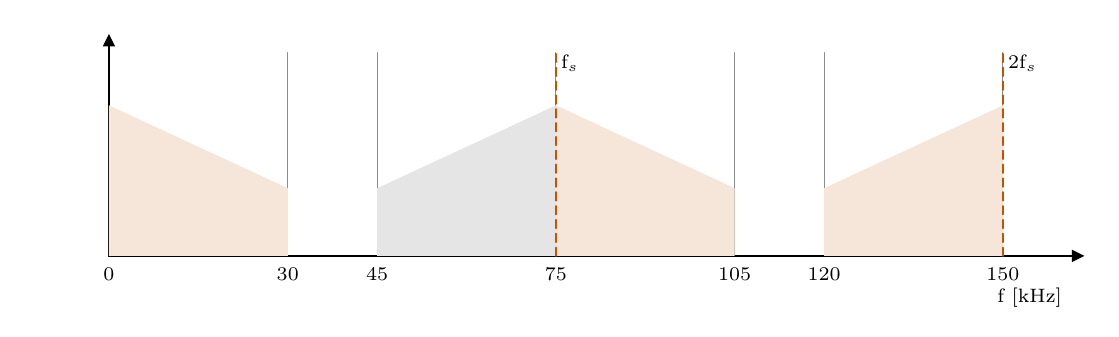
\begin{tikzpicture}[x=0.01985cm,y=-0.01985cm,line cap=round,line join=round]
\useasboundingbox (0,0) rectangle (680,180);
\path[draw=black!45,line width=0.35pt] (52,146) -- (52,16);
\path[draw=black!45,line width=0.35pt] (166.4,146) -- (166.4,16);
\path[draw=black!45,line width=0.35pt] (223.6,146) -- (223.6,16);
\path[draw=black!45,line width=0.35pt] (337.9,146) -- (337.9,16);
\path[draw=black!45,line width=0.35pt] (452.3,146) -- (452.3,16);
\path[draw=black!45,line width=0.35pt] (509.5,146) -- (509.5,16);
\path[draw=black!45,line width=0.35pt] (623.9,146) -- (623.9,16);
\path[draw=black,line width=0.7pt] (52,146) -- (670,146);
\path[fill=black,draw=none] (676,146) -- (668,142) -- (668,150) -- cycle;
\path[draw=black,line width=0.7pt] (52,146) -- (52,10);
\path[fill=black,draw=none] (52,4) -- (48,12) -- (56,12) -- cycle;
\node[anchor=base,inner sep=0pt,font=\scriptsize] at (52,162) {0};
\node[anchor=base,inner sep=0pt,font=\scriptsize] at (166.4,162) {30};
\node[anchor=base,inner sep=0pt,font=\scriptsize] at (223.6,162) {45};
\node[anchor=base,inner sep=0pt,font=\scriptsize] at (337.9,162) {75};
\node[anchor=base,inner sep=0pt,font=\scriptsize] at (452.3,162) {105};
\node[anchor=base,inner sep=0pt,font=\scriptsize] at (509.5,162) {120};
\node[anchor=base,inner sep=0pt,font=\scriptsize] at (623.9,162) {150};
\node[anchor=base east,inner sep=0pt,font=\scriptsize] at (662,176) {f [kHz]};
\path[fill=cB!15,draw=none] (52,146) -- (52,49.7) -- (166.4,102.7) -- (166.4,146) -- cycle;
\path[fill=black!10,draw=none] (223.6,146) -- (223.6,102.7) -- (337.9,49.7) -- (337.9,146) -- cycle;
\path[fill=cB!15,draw=none] (337.9,146) -- (337.9,49.7) -- (452.3,102.7) -- (452.3,146) -- cycle;
\path[fill=cB!15,draw=none] (509.5,146) -- (509.5,102.7) -- (623.9,49.7) -- (623.9,146) -- cycle;
\path[draw=cB,line width=0.8pt,dash pattern=on 3pt off 2pt] (337.9,146) -- (337.9,16);
\node[anchor=base west,inner sep=0pt,font=\scriptsize] at (340.9,26) {f$_s$};
\path[draw=cB,line width=0.8pt,dash pattern=on 3pt off 2pt] (623.9,146) -- (623.9,16);
\node[anchor=base west,inner sep=0pt,font=\scriptsize] at (626.9,26) {2f$_s$};
\end{tikzpicture}\end{center}
\begin{itemize}
\item Kék: az eredeti 45\ldots{}75 kHz-es sáv. Piros: a képek $n\cdot75\pm(45\ldots75)$ kHz-en: 0\ldots{}30, 75\ldots{}105, 120\ldots{}150 kHz.
\item A $75-f$ és $150-f$ képek tükrözöttek (a ferde tető csak ezt jelzi, a valódi alak tetszőleges). A 75\ldots{}105 kHz-es kép épp érinti az eredetit.
\end{itemize}
\end{rajz}
\begin{figyelem}[Javítás]
A példatár korábbi változata a képeket „0\ldots{}30, 105\ldots{}120 kHz”-nek írta: helyesen 0\ldots{}30, 75\ldots{}105, 120\ldots{}150 kHz.
\end{figyelem}
\begin{eredmeny}

\begin{center}\adjustbox{max width=\linewidth}{$\displaystyle \text{a) }f_s\ge150\ \text{kHz}\qquad\text{b) }75\le f_s\le90\ \text{kHz}\qquad\text{c) }f_{s,\min}=75\ \text{kHz},\ \text{képek }0\ldots30,\ 75\ldots105,\ 120\ldots150\ \text{kHz}$}\end{center}
\end{eredmeny}
\begin{tipp}[Ellenőrzés]
\begin{itemize}
\item A hallgatói megoldás ugyanezt a tartományt adja ($f_s-45\le45$, $2f_s-75\ge75$).
\end{itemize}
\end{tipp}


% ------------------------------------------------------------------
\section{\texorpdfstring{2.3. feladat: 60\ldots{}108 kHz-es jel: mintavételi frekvenciák és spektrum}{2.3. feladat: 60…108 kHz-es jel: mintavételi frekvenciák és spektrum}}\label{ai2_03}
\setcounter{lepes}{0}
\begin{feladat}{2.3. feladat}
Egy 60 és 108 kHz közötti komponensekből álló jelet közvetlenül digitalizálunk. a) Melyek a büntetlenül választható mintavételi frekvenciák? b) Milyen szűrők kellenek? c) Rajzolja fel a mintasorozat spektrumát egy célszerű $f_s$-sel!

{\footnotesize\sffamily Forrás: ALL-IN 55\ldots{}56., 80\ldots{}81., 93., 94., 97. oldal $\cdot$ ai2014\_12\_15\_4, ai2014\_01\_14\_2, aiD\_2\_2, aiD\_2\_5, aiD\_2\_12. Címkék: vizsga}
\end{feladat}
\begin{keresunk}
\begin{itemize}
\item a) $f_s$ (mintavételi frekvencia) tartományai
\item b) a szűrők
\item c) a spektrum
\end{itemize}
\end{keresunk}
\begin{jeloles}
\begin{jeltabla}
$\ca{f_L}$ & a jel legkisebb frekvenciája & $60$\,kHz\\
$\cb{f_H}$ & a jel legnagyobb frekvenciája & $108$\,kHz\\
$f_s$ & mintavételi frekvencia & \emph{keresett}\\
$k$ & a Nyquist-zóna sorszáma: a frekvenciatengelyt $f_s/2$ széles sávokra osztjuk, és $k$ annak a sávnak a sorszáma, amelybe a jel teljes sávja beleesik & \\
$B$ & a jel sávszélessége & \\
$k_{\max}$ & a legnagyobb szóba jöhető zónasorszám, $\lfloor f_H/B\rfloor$ & \\
$n$ & a kvantáló bitszáma & \\
\end{jeltabla}
\end{jeloles}
\begin{elmelet}[Miért így? Egyszerűen]
\textbf{Miért nem lehet $f_s=96$ kHz $(=2B)$?}\par A legkisebb elvi érték csak akkor $2B$, ha $f_H$ a $B$ egész többszöröse. Itt $108/48=2{,}25$, ezért a $k=2$-es tartomány alja $108$ kHz.
\end{elmelet}

\lepes{Mit jelent a $k$? A Nyquist-zóna sorszáma}
A mintavétel után a spektrum $f_s$-enként ismétlődik. Osszuk fel a frekvenciatengelyt $f_s/2$ széles sávokra (Nyquist-zónákra): $0\ldots f_s/2$ az első, $f_s/2\ldots f_s$ a második, és így tovább. \textbf{$k$ annak a zónának a sorszáma, amelybe a jel teljes sávja beleesik:} $(k-1)\,f_s/2\le {\ca{f_L}}$ és ${\cb{f_H}}\le k\,f_s/2$. A két egyenlőtlenséget $f_s$-re rendezve kapjuk a megengedett tartományt, $2{\cb{f_H}}/k\le f_s\le2{\ca{f_L}}/(k-1)$. A $k=1$ eset a szokásos aluláteresztő mintavétel ($f_s\ge2{\cb{f_H}}$). Mivel a zóna nem lehet keskenyebb a jelnél ($f_s/2\ge B$), $k$ legfeljebb ${\cb{f_H}}/B$ lehet, lefelé kerekítve: $k_{\max}=\lfloor {\cb{f_H}}/B\rfloor$.

\lepes{a) Tartományok}


\begin{center}\adjustbox{max width=\linewidth}{$\displaystyle B=48\ \text{kHz}\qquad\lfloor{\cb{108}}/48\rfloor=2$}\end{center}
\jegyzet{számérték}{}
\behely{\bh{\ca{f_L}}{\ca{60\un{kHz}}} \bh{\cb{f_H}}{\cb{108\un{kHz}}}}

\begin{center}\adjustbox{max width=\linewidth}{$\displaystyle k=1:\ f_s\ge216\ \text{kHz}\qquad k=2:\ \frac{216}{2}={\cb{108}}\le f_s\le\frac{2\cdot{\ca{60}}}{1}=120\ \text{kHz}$}\end{center}
\jegyzet{behelyettesítés}{}

\lepes{b) Szűrők}
$k=1$ ($f_s\ge216$ kHz): elő- és utószűrő is 108 kHz-es aluláteresztő. $k=2$ (${\cb{108}}\ldots120$ kHz): mindkettő 60\ldots{}108 kHz-es sávszűrő, mert az alapsávban (6\ldots{}54 kHz) is lesz kép.

\lepes{c) Spektrum $f_s=114$ kHz-nél}
A tartomány közepét választjuk, hogy mindkét oldalon legyen tartalék. Képek $n\cdot114\pm({\ca{60}}\ldots{\cb{108}})$:

\begin{center}\adjustbox{max width=\linewidth}{$\displaystyle 6\ldots54,\ \mathbf{60\ldots{\cb{108}}},\ 120\ldots168,\ 174\ldots222,\ 234\ldots282,\ 288\ldots336\ \text{kHz}$}\end{center}
\jegyzet{számérték}{nincs átfedés, 6 kHz-es rések}

\begin{rajz}
\textbf{A mintasorozat spektruma f\_s = 114 kHz-nél}\par
\begin{center}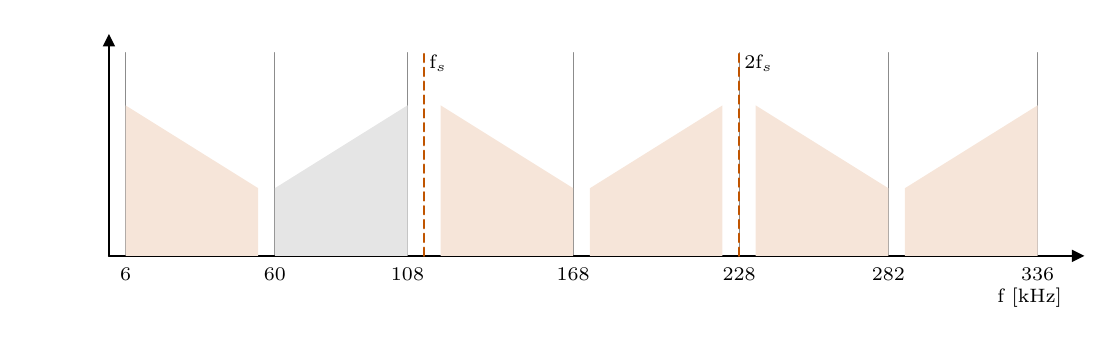
\begin{tikzpicture}[x=0.01985cm,y=-0.01985cm,line cap=round,line join=round]
\useasboundingbox (0,0) rectangle (680,180);
\path[draw=black!45,line width=0.35pt] (62.6,146) -- (62.6,16);
\path[draw=black!45,line width=0.35pt] (158.1,146) -- (158.1,16);
\path[draw=black!45,line width=0.35pt] (243,146) -- (243,16);
\path[draw=black!45,line width=0.35pt] (349,146) -- (349,16);
\path[draw=black!45,line width=0.35pt] (455.1,146) -- (455.1,16);
\path[draw=black!45,line width=0.35pt] (550.6,146) -- (550.6,16);
\path[draw=black!45,line width=0.35pt] (646.1,146) -- (646.1,16);
\path[draw=black,line width=0.7pt] (52,146) -- (670,146);
\path[fill=black,draw=none] (676,146) -- (668,142) -- (668,150) -- cycle;
\path[draw=black,line width=0.7pt] (52,146) -- (52,10);
\path[fill=black,draw=none] (52,4) -- (48,12) -- (56,12) -- cycle;
\node[anchor=base,inner sep=0pt,font=\scriptsize] at (62.6,162) {6};
\node[anchor=base,inner sep=0pt,font=\scriptsize] at (158.1,162) {60};
\node[anchor=base,inner sep=0pt,font=\scriptsize] at (243,162) {108};
\node[anchor=base,inner sep=0pt,font=\scriptsize] at (349,162) {168};
\node[anchor=base,inner sep=0pt,font=\scriptsize] at (455.1,162) {228};
\node[anchor=base,inner sep=0pt,font=\scriptsize] at (550.6,162) {282};
\node[anchor=base,inner sep=0pt,font=\scriptsize] at (646.1,162) {336};
\node[anchor=base east,inner sep=0pt,font=\scriptsize] at (662,176) {f [kHz]};
\path[fill=cB!15,draw=none] (62.6,146) -- (62.6,49.7) -- (147.5,102.7) -- (147.5,146) -- cycle;
\path[fill=black!10,draw=none] (158.1,146) -- (158.1,102.7) -- (243,49.7) -- (243,146) -- cycle;
\path[fill=cB!15,draw=none] (264.2,146) -- (264.2,49.7) -- (349,102.7) -- (349,146) -- cycle;
\path[fill=cB!15,draw=none] (359.7,146) -- (359.7,102.7) -- (444.5,49.7) -- (444.5,146) -- cycle;
\path[fill=cB!15,draw=none] (465.7,146) -- (465.7,49.7) -- (550.6,102.7) -- (550.6,146) -- cycle;
\path[fill=cB!15,draw=none] (561.2,146) -- (561.2,102.7) -- (646.1,49.7) -- (646.1,146) -- cycle;
\path[draw=cB,line width=0.8pt,dash pattern=on 3pt off 2pt] (253.6,146) -- (253.6,16);
\node[anchor=base west,inner sep=0pt,font=\scriptsize] at (256.6,26) {f$_s$};
\path[draw=cB,line width=0.8pt,dash pattern=on 3pt off 2pt] (455.1,146) -- (455.1,16);
\node[anchor=base west,inner sep=0pt,font=\scriptsize] at (458.1,26) {2f$_s$};
\end{tikzpicture}\end{center}
\begin{itemize}
\item Kék: az eredeti 60\ldots{}108 kHz. Piros: a képek, felváltva tükrözve, 6 kHz-es résekkel. Sehol nincs átfedés.
\end{itemize}
\end{rajz}
\begin{eredmeny}

\begin{center}\adjustbox{max width=\linewidth}{$\displaystyle \text{a) }f_s\ge216\ \text{kHz},\ \text{vagy}\ 108\le f_s\le120\ \text{kHz}\qquad\text{b) 108 kHz-es aluláteresztő, illetve 60\ldots{}108 kHz-es sávszűrő}$}\end{center}
\end{eredmeny}
\begin{tipp}[Ellenőrzés]
\begin{itemize}
\item Ugyanez a feladat öt helyen szerepel a gyűjteményben, mindenhol ezzel az eredménnyel, az egyik hivatalos (aláírt) kézírással.
\end{itemize}
\end{tipp}


% ------------------------------------------------------------------
\section{\texorpdfstring{2.4. feladat: 60\ldots{}108 kHz-es jel: hány bit kell?}{2.4. feladat: 60…108 kHz-es jel: hány bit kell?}}\label{ai2_04}
\setcounter{lepes}{0}
\begin{feladat}{2.4. feladat}
Egy 60 és 108 kHz közötti komponensekből álló jelet közvetlenül digitalizálunk, egyenletes kvantálóval. a) $C=\sqrt3$, legalább 70 dB SNR. b) Szinuszos jel, 70 dB, minden választható tartományra. c) $C=\sqrt6$, $f_s=432$ kHz, legalább 60 dB. Hány bites egyenletes kvantáló kell?

{\footnotesize\sffamily Forrás: ALL-IN 56\ldots{}57., 81\ldots{}82., 94\ldots{}95. oldal $\cdot$ ai2014\_12\_15\_4, ai2014\_01\_14\_2, aiD\_2\_2 d), aiD\_2\_5 b). Címkék: vizsga, javítás}
\end{feladat}
\begin{keresunk}
\begin{itemize}
\item $n$ (a kvantáló bitszáma) a három esetben
\end{itemize}
\end{keresunk}
\begin{jeloles}
\begin{jeltabla}
$\ca{B}$ & a jel sávszélessége & $48$\,kHz\\
$f_H$ & a jel legnagyobb frekvenciája & \\
$\cb{k}$ & a Nyquist-zóna sorszáma & $1$\\
$f_s$ & mintavételi frekvencia & \\
$f_L$ & a jel legkisebb frekvenciája & \\
$n$ & a kvantáló bitszáma & \emph{keresett}\\
$C$ & csúcstényező & \\
$B_z$ & a visszaállító szűrő sávszélessége (ennyi zajt enged át) & \\
\end{jeltabla}
\end{jeloles}

\lepes{a) Háromszögjel, 70 dB}
$10\lg(3/C^2)=10\lg1=0$. A $108\ldots120$ kHz-es tartományban sávszűrővel ($B_z={\ca{48}}$ kHz) a túlmintavételezés $10\lg(f_s/96)=0{,}5\ldots1$ dB.

\begin{center}\adjustbox{max width=\linewidth}{$\displaystyle 0+0{,}5+6{,}02\,n\ge70\ \Rightarrow\ n\ge\frac{69{,}5}{6{,}02}=11{,}5$}\end{center}
\jegyzet{behelyettesítés}{$f_s=108$ kHz, a legrosszabb eset}

\begin{center}\adjustbox{max width=\linewidth}{$\displaystyle n=12$}\end{center}
\jegyzet{számérték}{}

\lepes{b) Szinusz, 70 dB}
$10\lg(3/2)=1{,}76$ dB.

\begin{center}\adjustbox{max width=\linewidth}{$\displaystyle 1{,}76+6{,}02\,n\ge70\ \Rightarrow\ n\ge11{,}3\ \Rightarrow\ 12$}\end{center}
\jegyzet{behelyettesítés}{túlmintavételezés nélkül}
\behely{\bh{\ca{B}}{\ca{48\un{kHz}}}}

\begin{center}\adjustbox{max width=\linewidth}{$\displaystyle f_s=216,\ B_z={\ca{48}}:\ 10\lg\frac{216}{96}=3{,}5\ \text{dB}\ \Rightarrow\ n\ge\frac{70-1{,}76-3{,}5}{6{,}02}=10{,}75\ \Rightarrow\ 11$}\end{center}
\jegyzet{behelyettesítés}{csak sávszűrős visszaállításnál}

\lepes{c) Csúcstényező $C=\sqrt6$, 432 kHz-es mintavétel, 60 dB}
A 60 dB teljesítményarány, $10^{60/10}=10^6$. Sávszűrővel $B_z={\ca{48}}$ kHz.

\begin{center}\adjustbox{max width=\linewidth}{$\displaystyle \frac{3}{6}\cdot\frac{432}{96}\cdot4^n\ge10^6\ \Rightarrow\ 2{,}25\cdot4^n\ge10^6\ \Rightarrow\ 4^n\ge444\,444$}\end{center}
\jegyzet{behelyettesítés}{$2^{2n}=4^n$}

\begin{center}\adjustbox{max width=\linewidth}{$\displaystyle n\ge\log_4444\,444=\frac{\lg444\,444}{\lg4}=9{,}4\ \Rightarrow\ n=10$}\end{center}
\jegyzet{átalakítás}{108 kHz-es aluláteresztővel is $9{,}97\to10$}
\begin{figyelem}[Javítás]
A c) részre a kézírás $n=8$-at ad, egy megjegyzés pedig $n=5$-öt („a 60 dB az 1000”). Mindkettő hibás: az SNR teljesítményarány, $10\lg$-gel számolandó. Az a) és b) indoklásában az „egyenletes kvantálónál $f_s=2B$” állítás pontatlan, a végeredményt nem rontja.
\end{figyelem}
\begin{eredmeny}

\begin{center}\adjustbox{max width=\linewidth}{$\displaystyle \text{a) }12\qquad\text{b) }12\ (f_s\ge216\ \text{kHz-nél sávszűrővel }11)\qquad\text{c) }10\ \text{bit}$}\end{center}
\end{eredmeny}
\begin{figyelem}[Tipikus hibák]
\begin{itemize}
\item $20\lg$-et használni a jel-zaj viszonyra.
\item Lefelé kerekíteni a bitszámot.
\end{itemize}
\end{figyelem}


% ------------------------------------------------------------------
\section{\texorpdfstring{2.5. feladat: 0\ldots{}3 és 7\ldots{}8 kHz-es jel: melyik $f_s$ jó?}{2.5. feladat: 0…3 és 7…8 kHz-es jel: melyik fs jó?}}\label{ai2_05}
\setcounter{lepes}{0}
\begin{feladat}{2.5. feladat}
Egy valós jel csak a 0\ldots{}3 kHz és a 7\ldots{}8 kHz közötti sávban tartalmaz komponenseket. Mely mintavételi frekvenciák mellett lehetséges a tökéletes visszaállítás? A) 13,6 kHz B) 16,2 kHz C) 15 kHz D) 10 kHz

{\footnotesize\sffamily Forrás: ALL-IN 94. oldal $\cdot$ aiD\_2\_3 (feleletválasztós 3.3.). Címkék: beugró}
\end{feladat}
\begin{keresunk}
\begin{itemize}
\item a jó $f_s$-ek (mintavételi frekvencia)
\end{itemize}
\end{keresunk}
\begin{jeloles}
\begin{jeltabla}
$f_s$ & mintavételi frekvencia & \emph{keresett}\\
\end{jeltabla}
\par\smallskip\textbf{Adott még:}
\begin{itemize}
\item két sáv: 0\ldots{}3 kHz és 7\ldots{}8 kHz, köztük 3\ldots{}7 kHz-es rés
\end{itemize}
\end{jeloles}

\lepes{A feltétel}
A legközelebbi képek $f_s-(0\ldots3)$ és $f_s-(7\ldots8)$. Egyik sem eshet a két sávra. Aluláteresztő visszaállításhoz $f_s\ge16$ kHz kell. Kisebb $f_s$-nél a $7\ldots8$ kHz képének a résbe kell esnie: $f_s-8\ge3$ és $f_s-7\le7$, azaz $11\le f_s\le14$ kHz (két áteresztősávú szűrővel).

\lepes{Az opciók}


\begin{center}\adjustbox{max width=\linewidth}{$\displaystyle A)\ 13{,}6:\ 5{,}6\ldots6{,}6\ \text{és}\ 10{,}6\ldots13{,}6\ \text{kHz}$}\end{center}
\jegyzet{ellenőrzés}{a résben és a sáv felett: jó}

\begin{center}\adjustbox{max width=\linewidth}{$\displaystyle B)\ 16{,}2>16$}\end{center}
\jegyzet{ellenőrzés}{jó}

\begin{center}\adjustbox{max width=\linewidth}{$\displaystyle C)\ 15-(7\ldots8)=7\ldots8$}\end{center}
\jegyzet{ellenőrzés}{a sáv önmagára fordul: rossz}

\begin{center}\adjustbox{max width=\linewidth}{$\displaystyle D)\ 10-8=2\ \text{kHz}\in0\ldots3$}\end{center}
\jegyzet{ellenőrzés}{rossz}
\begin{eredmeny}

\begin{center}\adjustbox{max width=\linewidth}{$\displaystyle \text{A és B}$}\end{center}
\end{eredmeny}


% ------------------------------------------------------------------
\section{\texorpdfstring{2.6. feladat: 4 kHz-es szinusz 8 kHz-es mintavétellel}{2.6. feladat: 4 kHz-es szinusz 8 kHz-es mintavétellel}}\label{ai2_06}
\setcounter{lepes}{0}
\begin{feladat}{2.6. feladat}
Visszaállítható-e egy 2 V-os 4 kHz-es jel, ha a mintavételi idő 125 \textmu{}s? És ha $\sqrt2$-ed részére csökkentjük?

{\footnotesize\sffamily Forrás: ALL-IN 94. oldal $\cdot$ aiD\_2\_4. Címkék: beugró, javítás}
\end{feladat}
\begin{keresunk}
\begin{itemize}
\item visszaállítható-e a két esetben
\end{itemize}
\end{keresunk}
\begin{jeloles}
\begin{jeltabla}
$\ca{f}$ & a bemenő jel frekvenciája & $4$\,kHz\\
$\cb{T_1}$ & első mintavételi idő & $125$\,\textmu{}s\\
$\cc{T_2}$ & második mintavételi idő & $88{,}4$\,\textmu{}s\\
$f_{s1}$ & az első mintavételi frekvencia, $1/T_1$ & \\
$x$ & a bemenő szinusz & \\
$k$ & a minta sorszáma & \\
$\varphi$ & a szinusz kezdőfázisa & \\
$f_{s2}$ & a második mintavételi frekvencia, $1/T_2$ & \\
\end{jeltabla}
\end{jeloles}

\lepes{Első eset}
A mintavételi frekvencia a mintavételi idő reciproka.

\begin{center}\adjustbox{max width=\linewidth}{$\displaystyle f_{s1}=\frac{1}{125\ \mu\text{s}}=8\ \text{kHz}=2{\ca{f}}$}\end{center}
\jegyzet{definíció}{éppen a határeset}

\begin{center}\adjustbox{max width=\linewidth}{$\displaystyle x(kT)=2\sin(2\pi\cdot4\cdot k\cdot0{,}125+\varphi)=2\sin(k\pi+\varphi)$}\end{center}
\jegyzet{ellenőrzés}{ha $\varphi=0$, minden minta 0}

\lepes{Második eset}


\begin{center}\adjustbox{max width=\linewidth}{$\displaystyle f_{s2}=\sqrt2\cdot8=11{,}3\ \text{kHz}>2\cdot4\ \text{kHz}$}\end{center}
\jegyzet{számérték}{visszaállítható}
\begin{figyelem}[Javítás]
A gyűjtemény szerint 8 kHz-nél „visszaállítható”. A tétel szigorú egyenlőtlenséget kíván: pontosan $f_s=2f$-nél a minták a szinusz nullátmeneteire is eshetnek. A második indoklásban „$f_{s2}>2f_{s1}$” elírás, helyesen $f_{s2}>2f$.
\end{figyelem}
\begin{eredmeny}

\begin{center}\adjustbox{max width=\linewidth}{$\displaystyle 8\ \text{kHz: nem biztosan (a fázistól függ)}\qquad 11{,}3\ \text{kHz: igen}$}\end{center}
\end{eredmeny}


% ------------------------------------------------------------------
\section{\texorpdfstring{2.7. feladat: Ferde szűrős rendszer: 10 és 8 kHz-es változat}{2.7. feladat: Ferde szűrős rendszer: 10 és 8 kHz-es változat}}\label{ai2_07}
\setcounter{lepes}{0}
\begin{feladat}{2.7. feladat}
A be- és kimenő szűrő azonos: $H=1$, ha $|f|\le5$ kHz, $H=3{,}5-|f|/2$, ha $5\le|f|\le7$ kHz ($f$ kHz-ben), egyébként 0. A bemenet 2 V-os 1 kHz-es és 3 V-os 6 kHz-es komponens. Mi jelenik meg a kimeneten, ha a) $f_s=10$ kHz (A: 6 kHz 0,75 V, B: 4 kHz, C: 6 kHz 0,5 V, D: 9 kHz), b) $f_s=8$ kHz (A: 6 kHz 3/4 V, B: 2 kHz 0,5 V, C: 4,5 kHz 0,5 V, D: 2 kHz 3/4 V)?

{\footnotesize\sffamily Forrás: ALL-IN 95., 97. oldal $\cdot$ aiD\_2\_6 (4.1.), aiD\_2\_15 (5.4.). Címkék: beugró}
\end{feladat}
\begin{keresunk}
\begin{itemize}
\item a), b) a kimenő összetevők
\end{itemize}
\end{keresunk}
\begin{jeloles}
\begin{jeltabla}
$H$ & a szűrő átvitele & \\
$f$ & a bemenő jel frekvenciája & \\
$f_s$ & mintavételi frekvencia & \\
\end{jeltabla}
\par\smallskip\textbf{Adott még:}
\begin{itemize}
\item $H(f)$: 5 kHz-ig 1, 5 és 7 kHz között lineárisan csökken 0-ra, felette 0
\item bemenet: 1 kHz, 2 V és 6 kHz, 3 V
\end{itemize}
\end{jeloles}

\lepes{Az előszűrő után}
Az 1 kHz átjut. A 6 kHz a ferde szakaszon van:

\begin{center}\adjustbox{max width=\linewidth}{$\displaystyle H(6)=3{,}5-\frac62=0{,}5\ \Rightarrow\ 3\cdot0{,}5=1{,}5\ \text{V}$}\end{center}
\jegyzet{behelyettesítés}{a mintavevőre jut}

\lepes{a) Mintavételi frekvencia $f_s=10$ kHz}
Képek: $10\pm1$, $10\pm6$, \ldots{} Az utószűrő ugyanaz a $H$.

\begin{center}\adjustbox{max width=\linewidth}{$\displaystyle 1\ \text{kHz: }2\ \text{V}\qquad6\ \text{kHz: }1{,}5\cdot0{,}5=0{,}75\ \text{V}\qquad10-6=4\ \text{kHz: }1{,}5\cdot1=1{,}5\ \text{V}$}\end{center}
\jegyzet{számérték}{}

\begin{center}\adjustbox{max width=\linewidth}{$\displaystyle 10-1=9\ \text{kHz: }H(9)=0$}\end{center}
\jegyzet{ellenőrzés}{D hamis, C hamis (0,75 V, nem 0,5)}

\lepes{b) Mintavételi frekvencia $f_s=8$ kHz}


\begin{center}\adjustbox{max width=\linewidth}{$\displaystyle 6\ \text{kHz: }0{,}75\ \text{V}\qquad8-6=2\ \text{kHz: }1{,}5\ \text{V}$}\end{center}
\jegyzet{számérték}{B és D hamis (1,5 V)}

\begin{center}\adjustbox{max width=\linewidth}{$\displaystyle 8-1=7\ \text{kHz: }H(7)=0$}\end{center}
\jegyzet{ellenőrzés}{C hamis, 4,5 kHz-es vonal nincs}
\begin{eredmeny}

\begin{center}\adjustbox{max width=\linewidth}{$\displaystyle \text{a) A és B}\qquad\text{b) csak A}$}\end{center}
\end{eredmeny}


% ------------------------------------------------------------------
\section{\texorpdfstring{2.8. feladat: 12 kHz-es rendszer: a szűrők mérése}{2.8. feladat: 12 kHz-es rendszer: a szűrők mérése}}\label{ai2_08}
\setcounter{lepes}{0}
\begin{feladat}{2.8. feladat}
$f_s=12$ kHz. A 2 V-os 2,5 kHz-es mérőjel kimenő 2,5 kHz-es összetevője 2 V, a 9,5 kHz-es csak 20 mV. b) Mekkora a 2 V-os 9,5 kHz-es bemenet hatására a kimenő 9,5 kHz-es összetevő, ha a 2,5 kHz-es összetevő 40 mV? c) Melyik elemet változtatnád, hogy a 9,5 kHz-es bemenet hatására keletkező 2,5 kHz-es összetevő csökkenjen?

{\footnotesize\sffamily Forrás: ALL-IN 95\ldots{}96. oldal $\cdot$ aiD\_2\_9. Címkék: vizsga}
\end{feladat}
\begin{keresunk}
\begin{itemize}
\item b) a 2. mérésnél a kimenő 9,5 kHz-es összetevő
\item c) mit kell változtatni
\end{itemize}
\end{keresunk}
\begin{jeloles}
\begin{jeltabla}
$\ca{f_s}$ & mintavételi frekvencia & $12$\,kHz\\
$H_\text{elő}$ & az előszűrő (bemenő szűrő) átvitele & \\
$H_\text{utó}$ & az utószűrő (visszaállító szűrő) átvitele & \\
$U$ & a kimenő 9,5 kHz-es összetevő amplitúdója & \\
$U_{9{,}5\,\text{kHz}}$ & a kimenő 9,5 kHz-es összetevő amplitúdója & \\
\end{jeltabla}
\par\smallskip\textbf{Adott még:}
\begin{itemize}
\item 1. mérés: be 2,5 kHz, 2 V $\to$ ki 2,5 kHz: 2 V, 9,5 kHz: 20 mV
\item 2. mérés: be 9,5 kHz, 2 V $\to$ ki 2,5 kHz: 40 mV
\end{itemize}
\end{jeloles}
\begin{elmelet}[Miért így? Egyszerűen]
\textbf{Miért lehet a két mérésből szűrőértéket kiolvasni?}\par Mert minden kimeneti amplitúdó két szűrőérték szorzata (A1). Az első mérés az utószűrőt adja 9,5 kHz-en, a második az előszűrőt 9,5 kHz-en.
\end{elmelet}

\lepes{Az utószűrő 9,5 kHz-en}
Az 1. mérésben a 9,5 kHz a 2,5 kHz képe (${\ca{12}}-2{,}5$). A 2,5 kHz-es kimenet 2 V, tehát a sávban mindkét szűrő 1.

\begin{center}\adjustbox{max width=\linewidth}{$\displaystyle 2\cdot H_\text{elő}(2{,}5)\cdot H_\text{utó}(9{,}5)=0{,}02\ \Rightarrow\ H_\text{utó}(9{,}5)=0{,}01$}\end{center}
\jegyzet{behelyettesítés}{$H_\text{elő}(2{,}5)=1$}

\lepes{Az előszűrő 9,5 kHz-en}
A 2. mérésben a 9,5 kHz-es bemenet ${\ca{12}}-9{,}5=2{,}5$ kHz-re lapolódik, ott az utószűrő 1.

\begin{center}\adjustbox{max width=\linewidth}{$\displaystyle 2\cdot H_\text{elő}(9{,}5)\cdot1=0{,}04\ \Rightarrow\ H_\text{elő}(9{,}5)=0{,}02$}\end{center}
\jegyzet{behelyettesítés}{}

\lepes{b) A keresett összetevő}
A 9,5 kHz-es bemenet saját vonala mindkét szűrőn 9,5 kHz-en megy át.

\begin{center}\adjustbox{max width=\linewidth}{$\displaystyle U=2\cdot0{,}02\cdot0{,}01=0{,}4\ \text{mV}$}\end{center}
\jegyzet{számérték}{}

\lepes{c) Mit változtassunk?}
Az átlapolódott 2,5 kHz-es összetevő az utószűrő áteresztősávjában van, azt az utószűrő nem tudja csillapítani. Csak az előszűrő 9,5 kHz-es csillapítását lehet növelni (meredekebb szűrő), vagy nagyobb ${\ca{f_s}}$-t választani, hogy a kép ne essen a sávba.
\begin{tipp}[A gyűjtemény megoldása]
A gyűjtemény c) válasza: „bemenő szűrő felső határfrekvenciája vagy a mintavételi frekvencia megnövelése”. Ez helyes irány.
\end{tipp}
\begin{eredmeny}

\begin{center}\adjustbox{max width=\linewidth}{$\displaystyle \text{b) }U_{9{,}5\,\text{kHz}}=0{,}4\ \text{mV}\qquad\text{c) az előszűrő (zárótartománybeli csillapítás), vagy nagyobb }f_s$}\end{center}
\end{eredmeny}


% ------------------------------------------------------------------
\section{\texorpdfstring{2.9. feladat: Előadásrögzítés: 4 kHz, 9 kHz, 14 bit (hivatalos megoldás)}{2.9. feladat: Előadásrögzítés: 4 kHz, 9 kHz, 14 bit (hivatalos megoldás)}}\label{ai2_09}
\setcounter{lepes}{0}
\begin{feladat}{2.9. feladat}
A „szuperjó” mikrofon jelét 4 kHz-es ideális aluláteresztőn át 9 kHz-es mintavételezéssel és 14 bites egyenletes kvantálással digitalizáljuk. a) Tökéletes-e a hanghűség? b) Ha nem, miért? c) Kell-e az előszűrő? d) Mi változik, ha minden minta legkisebb 6 bitjét elhagyjuk? e) Hányszoros teljesítmény kell 26 dB-lel hangosabb beszédhez?

{\footnotesize\sffamily Forrás: ALL-IN 96\ldots{}97. oldal $\cdot$ aiD\_2\_11. Címkék: vizsga}
\end{feladat}
\begin{keresunk}
\begin{itemize}
\item a), b), c) szöveges válaszok
\item d) a jel-zaj viszony változása
\item e) teljesítményarány
\end{itemize}
\end{keresunk}
\begin{jeloles}
\begin{jeltabla}
$\ca{f_s}$ & mintavételi frekvencia & $9$\,kHz\\
$\cb{n}$ & a kvantáló bitszáma & $14$\,bit\\
\end{jeltabla}
\par\smallskip\textbf{Adott még:}
\begin{itemize}
\item 4 kHz-es ideális aluláteresztő a mikrofon után
\end{itemize}
\end{jeloles}

\lepes{a), b) Tökéletes-e?}
Nem. A 4 kHz feletti beszédösszetevők (sziszegő hangok) elvesznek, és a 14 bites kvantálás is ad (kicsi) zajt. Átlapolódás nincs, mert $9>2\cdot4$ kHz, és a D/A utáni szűrés sem ok (ezekért a javító pontot vont le).

\lepes{c) Előszűrő}
Kell. A 4 kHz-es szűrő éppen ez: nélküle a ${\ca{f_s}}/2=4{,}5$ kHz feletti hangok és zajok visszalapolódnának a hasznos sávba.

\lepes{d) 6 bit elhagyása}
Minden bit 6,02 dB-t ér (A3), 6 bit elhagyása 8 bites kvantálást jelent.

\begin{center}\adjustbox{max width=\linewidth}{$\displaystyle \Delta\text{SNR}=6\cdot6{,}02=36{,}1\ \text{dB}\qquad2^{2\cdot6}=4096$}\end{center}
\jegyzet{számérték}{a zajteljesítmény kb. 4000-szeres, hallható sistergés}

\lepes{e) 26 dB}
A dB teljesítményarány, $10\lg$-ből visszafelé:

\begin{center}\adjustbox{max width=\linewidth}{$\displaystyle 10^{26/10}=10^{2{,}6}=398\approx400$}\end{center}
\jegyzet{átalakítás}{fejben: $26=20+6$ dB, $100\cdot4=400$}
\begin{eredmeny}

\begin{center}\adjustbox{max width=\linewidth}{$\displaystyle \text{a) nem}\quad\text{c) igen}\quad\text{d) a zaj kb. 36 dB-lel nő}\quad\text{e) kb. 400-szoros}$}\end{center}
\end{eredmeny}


% ------------------------------------------------------------------
\section{\texorpdfstring{2.10. feladat: 70\ldots{}100 kHz-es jel}{2.10. feladat: 70…100 kHz-es jel}}\label{ai2_10}
\setcounter{lepes}{0}
\begin{feladat}{2.10. feladat}
Egy jel 70 és 100 kHz között tartalmaz komponenseket. Milyen mintavételi frekvenciák választhatók?

{\footnotesize\sffamily Forrás: ALL-IN 97. oldal $\cdot$ aiD\_2\_13. Címkék: vizsga}
\end{feladat}
\begin{keresunk}
\begin{itemize}
\item az $f_s$ (mintavételi frekvencia) tartományai
\end{itemize}
\end{keresunk}
\begin{jeloles}
\begin{jeltabla}
$\ca{f_L}$ & a jel legkisebb frekvenciája & $70$\,kHz\\
$\cb{f_H}$ & a jel legnagyobb frekvenciája & $100$\,kHz\\
$f_s$ & mintavételi frekvencia & \emph{keresett}\\
$k$ & a Nyquist-zóna sorszáma: a frekvenciatengelyt $f_s/2$ széles sávokra osztjuk, és $k$ annak a sávnak a sorszáma, amelybe a jel teljes sávja beleesik & \\
$B$ & a jel sávszélessége & \\
$k_{\max}$ & a legnagyobb szóba jöhető zónasorszám, $\lfloor f_H/B\rfloor$ & \\
\end{jeltabla}
\end{jeloles}

\lepes{Mit jelent a $k$? A Nyquist-zóna sorszáma}
A mintavétel után a spektrum $f_s$-enként ismétlődik. Osszuk fel a frekvenciatengelyt $f_s/2$ széles sávokra (Nyquist-zónákra): $0\ldots f_s/2$ az első, $f_s/2\ldots f_s$ a második, és így tovább. \textbf{$k$ annak a zónának a sorszáma, amelybe a jel teljes sávja beleesik:} $(k-1)\,f_s/2\le {\ca{f_L}}$ és ${\cb{f_H}}\le k\,f_s/2$. A két egyenlőtlenséget $f_s$-re rendezve kapjuk a megengedett tartományt, $2{\cb{f_H}}/k\le f_s\le2{\ca{f_L}}/(k-1)$. A $k=1$ eset a szokásos aluláteresztő mintavétel ($f_s\ge2{\cb{f_H}}$). Mivel a zóna nem lehet keskenyebb a jelnél ($f_s/2\ge B$), $k$ legfeljebb ${\cb{f_H}}/B$ lehet, lefelé kerekítve: $k_{\max}=\lfloor {\cb{f_H}}/B\rfloor$.

\lepes{Hány zóna jöhet szóba?}
A jel sávszélessége $B={\cb{f_H}}-{\ca{f_L}}$, és $k$ legfeljebb $\lfloor {\cb{f_H}}/B\rfloor$ lehet.

\begin{center}\adjustbox{max width=\linewidth}{$\displaystyle B=30\ \text{kHz}\qquad\lfloor100/30\rfloor=\lfloor3{,}33\rfloor=3$}\end{center}
\jegyzet{számérték}{$k=1,2,3$}

\lepes{Tartományok}
Behelyettesítés a sáváteresztő mintavétel képletébe, $2{\cb{f_H}}/k\le f_s\le2{\ca{f_L}}/(k-1)$:

\begin{center}\adjustbox{max width=\linewidth}{$\displaystyle k=1:\ f_s\ge200\qquad k=2:\ \frac{200}{2}=100\le f_s\le\frac{140}{1}=140$}\end{center}
\jegyzet{behelyettesítés}{kHz}
\behely{\bh{\ca{f_L}}{\ca{70\un{kHz}}}}

\begin{center}\adjustbox{max width=\linewidth}{$\displaystyle k=3:\ \frac{200}{3}=66{,}7\le f_s\le\frac{140}{2}={\ca{70}}$}\end{center}
\jegyzet{behelyettesítés}{kHz}
\begin{tipp}[A gyűjtemény megoldása]
A kézírás táblázatos próbálgatással a 66,7 kHz-et találja meg („itt csak sávszűrővel”), a $k=2$-es tartományt nem írja le.
\end{tipp}
\begin{eredmeny}

\begin{center}\adjustbox{max width=\linewidth}{$\displaystyle f_s\ge200\ \text{kHz}\qquad100\ldots140\ \text{kHz}\qquad66{,}7\ldots70\ \text{kHz}$}\end{center}
\end{eredmeny}


% ------------------------------------------------------------------
\section{\texorpdfstring{2.11. feladat: 19\ldots{}25 kHz-es jel: feleletválasztós}{2.11. feladat: 19…25 kHz-es jel: feleletválasztós}}\label{ai2_11}
\setcounter{lepes}{0}
\begin{feladat}{2.11. feladat}
Egy valós jel csak 19 és 25 kHz között tartalmaz komponenseket. Mely $f_s$ mellett lehetséges a tökéletes visszaállítás? A) 12,6 B) 11 C) 50,75 D) 39 kHz

{\footnotesize\sffamily Forrás: ALL-IN 98. oldal $\cdot$ aiD\_2\_16 (5.6.). Címkék: beugró}
\end{feladat}
\begin{keresunk}
\begin{itemize}
\item a jó $f_s$-ek (mintavételi frekvencia)
\end{itemize}
\end{keresunk}
\begin{jeloles}
\begin{jeltabla}
$\ca{f_L}$ & a jel legkisebb frekvenciája & $19$\,kHz\\
$\cb{f_H}$ & a jel legnagyobb frekvenciája & $25$\,kHz\\
$f_s$ & mintavételi frekvencia & \emph{keresett}\\
$k$ & a Nyquist-zóna sorszáma: a frekvenciatengelyt $f_s/2$ széles sávokra osztjuk, és $k$ annak a sávnak a sorszáma, amelybe a jel teljes sávja beleesik & \\
$B$ & a jel sávszélessége & \\
$k_{\max}$ & a legnagyobb szóba jöhető zónasorszám, $\lfloor f_H/B\rfloor$ & \\
\end{jeltabla}
\end{jeloles}

\lepes{Mit jelent a $k$? A Nyquist-zóna sorszáma}
A mintavétel után a spektrum $f_s$-enként ismétlődik. Osszuk fel a frekvenciatengelyt $f_s/2$ széles sávokra (Nyquist-zónákra): $0\ldots f_s/2$ az első, $f_s/2\ldots f_s$ a második, és így tovább. \textbf{$k$ annak a zónának a sorszáma, amelybe a jel teljes sávja beleesik:} $(k-1)\,f_s/2\le {\ca{f_L}}$ és ${\cb{f_H}}\le k\,f_s/2$. A két egyenlőtlenséget $f_s$-re rendezve kapjuk a megengedett tartományt, $2{\cb{f_H}}/k\le f_s\le2{\ca{f_L}}/(k-1)$. A $k=1$ eset a szokásos aluláteresztő mintavétel ($f_s\ge2{\cb{f_H}}$). Mivel a zóna nem lehet keskenyebb a jelnél ($f_s/2\ge B$), $k$ legfeljebb ${\cb{f_H}}/B$ lehet, lefelé kerekítve: $k_{\max}=\lfloor {\cb{f_H}}/B\rfloor$.

\lepes{Tartományok}


\begin{center}\adjustbox{max width=\linewidth}{$\displaystyle B=6\ \text{kHz}\qquad\lfloor{\cb{25}}/6\rfloor=4$}\end{center}
\jegyzet{számérték}{}
\behely{\bh{\ca{f_L}}{\ca{19\un{kHz}}} \bh{\cb{f_H}}{\cb{25\un{kHz}}}}

\begin{center}\adjustbox{max width=\linewidth}{$\displaystyle k=1:\ \ge50\quad k=2:\ {\cb{25}}\ldots38\quad k=3:\ 16{,}7\ldots{\ca{19}}\quad k=4:\ 12{,}5\ldots12{,}67$}\end{center}
\jegyzet{behelyettesítés}{kHz, pl. $k=4$: $50/4$ és $38/3$}

\lepes{Az opciók}


\begin{center}\adjustbox{max width=\linewidth}{$\displaystyle 12{,}6\in[12{,}5;\ 12{,}67]\qquad50{,}75\ge50$}\end{center}
\jegyzet{ellenőrzés}{A és C jó}

\begin{center}\adjustbox{max width=\linewidth}{$\displaystyle 11<12{,}5\qquad38<39<50$}\end{center}
\jegyzet{ellenőrzés}{B és D rossz}
\begin{eredmeny}

\begin{center}\adjustbox{max width=\linewidth}{$\displaystyle \text{A és C}$}\end{center}
\end{eredmeny}


% ------------------------------------------------------------------
\section{\texorpdfstring{2.12. feladat: 40\ldots{}70 kHz, 64 dB (Moodle-vizsga 2020)}{2.12. feladat: 40…70 kHz, 64 dB (Moodle-vizsga 2020)}}\label{ai2_12}
\setcounter{lepes}{0}
\begin{feladat}{2.12. feladat}
Valós, $\sqrt2$ csúcstényezőjű, teljes kivezérlésű jel, 40 és 70 kHz között, legalább 64 dB SNR. a) Az összes átlapolódásmentes $f_s$. b) Szűrők. c) Hány bit, ha aluláteresztőkkel állítjuk vissza?

{\footnotesize\sffamily Forrás: ALL-IN 16. oldal $\cdot$ ai2020\_06\_02\_Q8. Címkék: vizsga}
\end{feladat}
\begin{keresunk}
\begin{itemize}
\item a) $f_s$ (mintavételi frekvencia)
\item b) szűrők
\item c) $n$ (a kvantáló bitszáma)
\end{itemize}
\end{keresunk}
\begin{jeloles}
\begin{jeltabla}
$\ca{f_L}$ & a jel legkisebb frekvenciája & $40$\,kHz\\
$\cb{f_H}$ & a jel legnagyobb frekvenciája & $70$\,kHz\\
$C$ & csúcstényező & \\
$f_s$ & mintavételi frekvencia & \emph{keresett}\\
$n$ & a kvantáló bitszáma & \emph{keresett}\\
$k$ & a Nyquist-zóna sorszáma: a frekvenciatengelyt $f_s/2$ széles sávokra osztjuk, és $k$ annak a sávnak a sorszáma, amelybe a jel teljes sávja beleesik & \\
$B$ & a jel sávszélessége & \\
$k_{\max}$ & a legnagyobb szóba jöhető zónasorszám, $\lfloor f_H/B\rfloor$ & \\
$B_z$ & a visszaállító szűrő sávszélessége (ennyi zajt enged át) & \\
\end{jeltabla}
\end{jeloles}

\lepes{Mit jelent a $k$? A Nyquist-zóna sorszáma}
A mintavétel után a spektrum $f_s$-enként ismétlődik. Osszuk fel a frekvenciatengelyt $f_s/2$ széles sávokra (Nyquist-zónákra): $0\ldots f_s/2$ az első, $f_s/2\ldots f_s$ a második, és így tovább. \textbf{$k$ annak a zónának a sorszáma, amelybe a jel teljes sávja beleesik:} $(k-1)\,f_s/2\le {\ca{f_L}}$ és ${\cb{f_H}}\le k\,f_s/2$. A két egyenlőtlenséget $f_s$-re rendezve kapjuk a megengedett tartományt, $2{\cb{f_H}}/k\le f_s\le2{\ca{f_L}}/(k-1)$. A $k=1$ eset a szokásos aluláteresztő mintavétel ($f_s\ge2{\cb{f_H}}$). Mivel a zóna nem lehet keskenyebb a jelnél ($f_s/2\ge B$), $k$ legfeljebb ${\cb{f_H}}/B$ lehet, lefelé kerekítve: $k_{\max}=\lfloor {\cb{f_H}}/B\rfloor$.

\lepes{a) Tartományok}


\begin{center}\adjustbox{max width=\linewidth}{$\displaystyle B=30\ \text{kHz}\qquad\lfloor{\cb{70}}/30\rfloor=2$}\end{center}
\jegyzet{számérték}{}
\behely{\bh{\cb{f_H}}{\cb{70\un{kHz}}}}

\begin{center}\adjustbox{max width=\linewidth}{$\displaystyle k=1:\ f_s\ge140\qquad k=2:\ {\cb{70}}\le f_s\le80\ \text{kHz}$}\end{center}
\jegyzet{behelyettesítés}{$140/2$ és $80/1$}

\lepes{b) Szűrők}
$f_s\ge140$ kHz: aluláteresztő (70 kHz-es) elő- és utószűrő. ${\cb{70}}\ldots80$ kHz: 40\ldots{}70 kHz-es sávszűrők.

\lepes{c) Bitszám}
Aluláteresztő visszaállításnál ($f_s=140$ kHz, $B_z={\cb{70}}$ kHz) nincs túlmintavételezési nyereség: $10\lg(140/140)=0$.

\begin{center}\adjustbox{max width=\linewidth}{$\displaystyle 1{,}76+6{,}02\,n\ge64\ \Rightarrow\ n\ge\frac{62{,}24}{6{,}02}=10{,}34$}\end{center}
\jegyzet{behelyettesítés}{}

\begin{center}\adjustbox{max width=\linewidth}{$\displaystyle n=11$}\end{center}
\jegyzet{számérték}{ellenőrzés: 11 bittel 68,0 dB, 10 bittel 62,0 dB}
\begin{eredmeny}

\begin{center}\adjustbox{max width=\linewidth}{$\displaystyle \text{a) }f_s\ge140\ \text{kHz vagy }70\ldots80\ \text{kHz}\qquad\text{b) aluláteresztő, illetve sávszűrő}\qquad\text{c) }n=11$}\end{center}
\end{eredmeny}
\begin{tipp}[Ellenőrzés]
\begin{itemize}
\item A javító teljes pontot adott.
\end{itemize}
\end{tipp}

% Generálva: html/build_tex.js (ai03.js). Kézzel ne szerkeszd, a forrás a html/data mappa.
\setcounter{chapter}{2}
\chapter{\texorpdfstring{Rádiós összeköttetések}{Rádiós összeköttetések}}\label{f3}
Szabadtéri (egyutas) és sík föld feletti (kétutas) terjedés, antennanyereség és hatásos felület. A kulcskérdés mindig az, hogy a vevő az interferenciazónán belül vagy azon túl van-e.

\section{Alapok, egyszerűen}
\subsection{\texorpdfstring{A1. Jelölések és egyutas (szabadtéri) terjedés}{A1. Jelölések és egyutas (szabadtéri) terjedés}}\label{a3-egyutas}
\par\noindent{\small\renewcommand{\arraystretch}{1.25}\begin{tabularx}{\linewidth}{@{}>{\raggedright\arraybackslash}X>{\raggedright\arraybackslash}X@{}}\toprule
\textbf{Jel} & \textbf{Jelentés}\\\midrule
undefined & adott és vett teljesítmény\\
undefined & adó- és vevőantenna-nyereség (dB-ben vagy szorzóként)\\
undefined & szakaszcsillapítás, undefined, az antennákkal együtt\\
undefined & hullámhossz, undefined, undefined m/s\\
undefined & távolság\\
undefined & az adó- és a vevőantenna magassága a visszaverő sík felett\\
undefined & a talaj reflexiós tényezője (tökéletes tükörnél undefined)\\
undefined & hatásos felület\\
\bottomrule\end{tabularx}}\par

\begin{center}\adjustbox{max width=\linewidth}{$\displaystyle a_\mathrm{sz}=20\lg\frac{4\pi r}{\lambda}-G_T^\mathrm{dB}-G_R^\mathrm{dB}$}\end{center}

A teljesítménysűrűség a távolság négyzetével csökken, a vevő ebből a hatásos felületével „merít”: $P_R=S\cdot A_h$.

\subsection{\texorpdfstring{A2. Kétutas terjedés sík föld felett}{A2. Kétutas terjedés sík föld felett}}\label{a3-ketutas}
A vevőbe a direkt és a földről visszavert hullám érkezik, az úthossz-különbség kb. $2h_Th_R/r$. Tökéletes tükörnél ($\Gamma=-1$):

\begin{center}\adjustbox{max width=\linewidth}{$\displaystyle |E_R|=2|E_0|\left|\sin\left(\frac{2\pi h_Th_R}{r\lambda}\right)\right|$}\end{center}

Az argumentum $\pi/2$-nél a legtávolabbi \textbf{maximum} (az interferenciazóna határa): $r=4h_Th_R/\lambda$. Az argumentum $\pi$-nél a legtávolabbi \textbf{kioltás}: $r=2h_Th_R/\lambda$. A zónán túl $\sin x\approx x$, és

\begin{center}\adjustbox{max width=\linewidth}{$\displaystyle a_\mathrm{sz}=20\lg\frac{r^2}{h_Th_R}-G_T^\mathrm{dB}-G_R^\mathrm{dB}$}\end{center}

Itt a csillapítás nem függ a frekvenciától, és a távolsággal 40 dB/dekád meredeken nő. Ha a föld nem tökéletes tükör, a két hullám nem oltja ki teljesen egymást: $E_{\max}/E_{\min}=(1+|\Gamma|)/(1-|\Gamma|)$.

\subsection{\texorpdfstring{A3. Antennanyereség és hatásos felület}{A3. Antennanyereség és hatásos felület}}\label{a3-antenna}
\begin{center}\adjustbox{max width=\linewidth}{$\displaystyle G=\frac{4\pi A_h}{\lambda^2}\qquad A_h=\frac{G\lambda^2}{4\pi}$}\end{center}

Parabolánál a hatásos felület közelítőleg a nyílás területe, $A_h\approx R^2\pi$.

% ------------------------------------------------------------------
\section{\texorpdfstring{3.1. feladat: Kétutas szakasz, 10 km, 300 MHz (Moodle 2020)}{3.1. feladat: Kétutas szakasz, 10 km, 300 MHz (Moodle 2020)}}\label{ai3_01}
\setcounter{lepes}{0}
\begin{feladat}{3.1. feladat}
$h_T=h_R=10$ m, $r=10$ km, $f=300$ MHz, $G_T=5$ dB, $G_R=3$ dB, tökéletes reflexió. a) Szakaszcsillapítás? b) A vevőantenna magasságának változtatásával mekkora $E_{\max}/E_{\min}$, ha $\Gamma=-0{,}8$?

{\footnotesize\sffamily Forrás: ALL-IN 1. oldal $\cdot$ ai2020\_05\_26\_Q1. Címkék: vizsga}
\end{feladat}
\begin{keresunk}
\begin{itemize}
\item a) $a_\mathrm{sz}$ (szakaszcsillapítás)
\item b) $E_{\max}/E_{\min}$: a legnagyobb és a legkisebb térerősség aránya, miközben a vevőantenna magasságát változtatjuk
\end{itemize}
\end{keresunk}
\begin{jeloles}
\begin{jeltabla}
$\ca{h_T}$ & az adóantenna magassága & $10$\,m\\
$h_R$ & a vevőantenna magassága & \\
$\cb{r}$ & az adó és a vevő távolsága & $10$\,km\\
$\cc{f}$ & vivőfrekvencia & $300$\,MHz\\
$\lambda$ & hullámhossz & \\
$\cd{G_T}$ & az adóantenna nyeresége & $5$\,dB\\
$\ce{G_R}$ & a vevőantenna nyeresége & $3$\,dB\\
$\Gamma$ & a talaj reflexiós tényezője & \\
$a_\mathrm{sz}$ & szakaszcsillapítás & \emph{keresett}\\
$r_0$ & a zónahatár távolsága & \\
\end{jeltabla}
\end{jeloles}

\lepes{Melyik zónában van a vevő?}
A zónahatár (a legtávolabbi térerősség-maximum) helye $r_0=4h_Th_R/\lambda$. Ha a vevő ennél messzebb van, a távoli zónában van.

\begin{center}\adjustbox{max width=\linewidth}{$\displaystyle \frac{4h_Th_R}{\lambda}=\frac{4\cdot10\cdot10}{1}=400\ \text{m}\ll10\ \text{km}$}\end{center}
\jegyzet{behelyettesítés}{távoli zóna, a kétutas képlet kell}

\lepes{a) Szakaszcsillapítás}
A távoli zónában a kétutas képlet érvényes: $a_\mathrm{sz}=20\lg\frac{r^2}{h_Th_R}-{\cd{G_T}}-{\ce{G_R}}$.

\begin{center}\adjustbox{max width=\linewidth}{$\displaystyle a_\mathrm{sz}=20\lg\frac{(10^4)^2}{10\cdot10}-5-3=20\lg10^6-8=120-8=112\ \text{dB}$}\end{center}
\jegyzet{behelyettesítés}{}

\lepes{b) Nem tökéletes reflexió}
A vevő magasságát változtatva a két hullám hol azonos, hol ellentétes fázisban adódik össze: a térerősség $1+|\Gamma|$ és $1-|\Gamma|$ között változik (a direkt hullámhoz képest).

\begin{center}\adjustbox{max width=\linewidth}{$\displaystyle \frac{E_{\max}}{E_{\min}}=\frac{1+0{,}8}{1-0{,}8}=\frac{1{,}8}{0{,}2}=9$}\end{center}
\jegyzet{definíció}{$20\lg9=19$ dB}
\begin{eredmeny}

\begin{center}\adjustbox{max width=\linewidth}{$\displaystyle \text{a) }a_\mathrm{sz}=112\ \text{dB}\qquad\text{b) }E_{\max}/E_{\min}=9$}\end{center}
\end{eredmeny}


% ------------------------------------------------------------------
\section{\texorpdfstring{3.2. feladat: Mezőkovácsháza: zóna, csillapítás, keverés (Moodle 2020)}{3.2. feladat: Mezőkovácsháza: zóna, csillapítás, keverés (Moodle 2020)}}\label{ai3_02}
\setcounter{lepes}{0}
\begin{feladat}{3.2. feladat}
Sík vidék, az adótorony 40 m magas (a talaj 96 m-rel a tengerszint felett), $f=83{,}3$ MHz FM, $f_\mathrm{KF}=10{,}7$ MHz. A vevő 650 m-re, 1 m magasan. a) Felső keverésnél az oszcillátor? b) Tükörfrekvencia? c) Túl van-e a vevő az interferenciazónán? d) Szakaszcsillapítás, ha $G_T=20$ dB, $G_R=10$ dB?

{\footnotesize\sffamily Forrás: ALL-IN 15. oldal $\cdot$ ai2020\_06\_02\_Q7. Címkék: vizsga, javítás}
\end{feladat}
\begin{keresunk}
\begin{itemize}
\item a) $f_\text{osc}$ (az oszcillátor frekvenciája)
\item b) $f_t$ (tükörfrekvencia)
\item c) a vevő helye a zónához képest
\item d) $a_\mathrm{sz}$ (szakaszcsillapítás)
\end{itemize}
\end{keresunk}
\begin{jeloles}
\begin{jeltabla}
$\ca{h_T}$ & az adóantenna magassága & $40$\,m\\
$\cb{h_R}$ & a vevőantenna magassága & $1$\,m\\
$\cc{r}$ & az adó és a vevő távolsága & $650$\,m\\
$\cd{f}$ & vivőfrekvencia & $83{,}3$\,MHz\\
$\lambda$ & hullámhossz & \\
$f_\mathrm{KF}$ & középfrekvencia & \\
$\ce{G_T}$ & az adóantenna nyeresége & $20$\,dB\\
$G_R$ & a vevőantenna nyeresége & $10$\,dB\\
$f_\text{osc}$ & az oszcillátor frekvenciája & \emph{keresett}\\
$f_t$ & tükörfrekvencia & \emph{keresett}\\
$a_\mathrm{sz}$ & szakaszcsillapítás & \emph{keresett}\\
$f_\mathrm{osc}$ & az oszcillátor frekvenciája & \\
$r_0$ & a zónahatár távolsága & \\
\end{jeltabla}
\end{jeloles}
\begin{elmelet}[Miért így? Egyszerűen]
\textbf{Miért 40 m és nem 136 m?}\par A kétutas modellben az antenna magassága a \textbf{visszaverő sík} fölött számít. Sík vidéken a talaj 96 m-es tengerszint feletti magassága érdektelen.
\end{elmelet}

\lepes{a), b) Keverés}
Felső keverésnél az oszcillátor $f_\mathrm{KF}$-fel a vett frekvencia felett van, a tükör még $f_\mathrm{KF}$-fel feljebb.
\behely{\bh{\cd{f}}{\cd{83{,}3\un{MHz}}}}

\begin{center}\adjustbox{max width=\linewidth}{$\displaystyle f_\mathrm{osc}={\cd{83{,}3}}+10{,}7=94\ \text{MHz}\qquad f_t=94+10{,}7=104{,}7\ \text{MHz}$}\end{center}
\jegyzet{behelyettesítés}{}

\lepes{c) Zóna}
A zónahatár (a legtávolabbi térerősség-maximum) helye $r_0=4h_Th_R/\lambda$. Ha a vevő ennél messzebb van, a távoli zónában van.
\behely{\bh{\ca{h_T}}{\ca{40\un{m}}}}

\begin{center}\adjustbox{max width=\linewidth}{$\displaystyle \frac{4h_Th_R}{\lambda}=\frac{4\cdot{\ca{40}}\cdot1}{3{,}6}=44{,}4\ \text{m}$}\end{center}
\jegyzet{behelyettesítés}{}

\begin{center}\adjustbox{max width=\linewidth}{$\displaystyle {\cc{650}}\ \text{m}>44{,}4\ \text{m}$}\end{center}
\jegyzet{ellenőrzés}{túl van a zónán}

\lepes{d) Kétutas csillapítás}
A távoli zónában a kétutas képlet érvényes.
\behely{\bh{\ce{G_T}}{\ce{20\un{dB}}}}

\begin{center}\adjustbox{max width=\linewidth}{$\displaystyle a_\mathrm{sz}={\ce{20}}\lg\frac{650^2}{40\cdot1}-{\ce{20}}-10={\ce{20}}\lg10\,562-30=80{,}5-30=50{,}5\ \text{dB}$}\end{center}
\jegyzet{behelyettesítés}{}
\begin{tipp}[A gyűjtemény megoldása]
A hallgató a zónahatárt 4265 m-nek kapta, és egyutas képlettel 37 dB-t. A javító a c) és d) részt „elszámolva” jelöléssel nem fogadta el.
\end{tipp}
\begin{figyelem}[Javítás]
A zónahatár 44,4 m, a vevő túl van rajta, ezért a kétutas képlet kell: kb. 50,5 dB. A b) indoklása („felső keverésnél messzebb a tükör”) pontatlan, a tükör mindkét keverésnél $2f_\mathrm{KF}$-re van a vett frekvenciától.
\end{figyelem}
\begin{eredmeny}

\begin{center}\adjustbox{max width=\linewidth}{$\displaystyle \text{a) }94\ \text{MHz}\qquad\text{b) }104{,}7\ \text{MHz}\qquad\text{c) túl van}\qquad\text{d) }a_\mathrm{sz}\approx50{,}5\ \text{dB}$}\end{center}
\end{eredmeny}


% ------------------------------------------------------------------
\section{\texorpdfstring{3.3. feladat: 900 MHz: ne legyen kioltás 1 km-en túl}{3.3. feladat: 900 MHz: ne legyen kioltás 1 km-en túl}}\label{ai3_03}
\setcounter{lepes}{0}
\begin{feladat}{3.3. feladat}
900 MHz, fix adó ($G_T=10$ dB), mozgó vevő ($G_R=3$ dB, $h_R=1{,}66$ m). a) Mekkora lehet $h_T$, ha 1 km-en túl nincs kioltás? b) Maximális távolság, ha a késleltetés legfeljebb 50 \textmu{}s? c) Szakaszcsillapítás ekkor? d) Adóteljesítmény, ha a vevő 100 pW alatt nem érzékel?

{\footnotesize\sffamily Forrás: ALL-IN 99\ldots{}100. oldal $\cdot$ aiD\_3\_1. Címkék: vizsga}
\end{feladat}
\begin{keresunk}
\begin{itemize}
\item a) $h_T$ (az adóantenna magassága)
\item b) $r_{\max}$ (a legnagyobb távolság)
\item c) $a_\mathrm{sz}$ (szakaszcsillapítás)
\item d) $P_T$ (adóteljesítmény)
\end{itemize}
\end{keresunk}
\begin{jeloles}
\begin{jeltabla}
$\ca{f}$ & vivőfrekvencia & $900$\,MHz\\
$\lambda$ & hullámhossz & \\
$\cb{G_T}$ & az adóantenna nyeresége & $10$\,dB\\
$\cc{G_R}$ & a vevőantenna nyeresége & $3$\,dB\\
$\cd{h_R}$ & a vevőantenna magassága & $1{,}66$\,m\\
$h_T$ & az adóantenna magassága & \emph{keresett}\\
$r_{\max}$ & a legnagyobb távolság & \emph{keresett}\\
$a_\mathrm{sz}$ & szakaszcsillapítás & \emph{keresett}\\
$P_T$ & adóteljesítmény & \emph{keresett}\\
$r$ & az adó és a vevő távolsága & \\
$c$ & a fénysebesség, $3\cdot10^8$ m/s & \\
$P_R$ & vett teljesítmény & \\
\end{jeltabla}
\par\smallskip\textbf{Adott még:}
\begin{itemize}
\item a legtávolabbi kioltás 1 km-en
\item a terjedési késleltetés legfeljebb 50 \textmu{}s
\item a vevő érzékenysége 100 pW
\end{itemize}
\end{jeloles}

\lepes{a) A legtávolabbi kioltás}
A kioltás ott van, ahol a szinusz argumentuma $\pi$ (A2): $r=2h_Th_R/\lambda$. Ezt egyenlővé tesszük 1 km-rel.

\begin{center}\adjustbox{max width=\linewidth}{$\displaystyle h_T=\frac{r\lambda}{2{\cd{h_R}}}=\frac{1000\cdot1/3}{2\cdot{\cd{1{,}66}}}=\frac{333{,}3}{3{,}32}\approx100\ \text{m}$}\end{center}
\jegyzet{geometria}{}

\lepes{b) Legnagyobb távolság}
A rádióhullám $c$ sebességgel terjed, 50 \textmu{}s alatt:

\begin{center}\adjustbox{max width=\linewidth}{$\displaystyle r=c\cdot50\ \mu\text{s}=3\cdot10^8\cdot5\cdot10^{-5}=15\ 000\ \text{m}=15\ \text{km}$}\end{center}
\jegyzet{behelyettesítés}{}

\lepes{c) Csillapítás 15 km-en}
15 km messze túl van a zónahatáron ($4h_Th_R/\lambda=2$ km), kétutas képlet.
\behely{\bh{\cd{h_R}}{\cd{1{,}66\un{m}}}}

\begin{center}\adjustbox{max width=\linewidth}{$\displaystyle a_\mathrm{sz}=20\lg\frac{(15\cdot10^3)^2}{100\cdot{\cd{1{,}66}}}-10-3=20\lg(1{,}36\cdot10^6)-13=122{,}6-13=109{,}6\ \text{dB}$}\end{center}
\jegyzet{behelyettesítés}{$\approx$ 110 dB}

\lepes{d) Adóteljesítmény}
$P_T=P_R\cdot10^{a_\mathrm{sz}/10}$, kerekítve 110 dB-lel.

\begin{center}\adjustbox{max width=\linewidth}{$\displaystyle P_T=100\ \text{pW}\cdot10^{11}=10^{-10}\cdot10^{11}=10\ \text{W}$}\end{center}
\jegyzet{számérték}{}
\begin{eredmeny}

\begin{center}\adjustbox{max width=\linewidth}{$\displaystyle \text{a) }h_T\approx100\ \text{m}\qquad\text{b) }r=15\ \text{km}\qquad\text{c) }a_\mathrm{sz}\approx110\ \text{dB}\qquad\text{d) }P_T\approx10\ \text{W}$}\end{center}
\end{eredmeny}
\begin{figyelem}[Tipikus hibák]
\begin{itemize}
\item A legtávolabbi kioltást a $4h_Th_R/\lambda$ képlettel keresni: az a legtávolabbi maximum.
\end{itemize}
\end{figyelem}


% ------------------------------------------------------------------
\section{\texorpdfstring{3.4. feladat: 450 MHz-es mobilrendszer (hivatalos megoldás)}{3.4. feladat: 450 MHz-es mobilrendszer (hivatalos megoldás)}}\label{ai3_04}
\setcounter{lepes}{0}
\begin{feladat}{3.4. feladat}
450 MHz, bázisállomás-antenna 50 m, vevők 1,5 m. a) Hol az interferenciazóna határa? b) A vevő magasságát változtatva mekkora $E_{\max}/E_{\min}$, ha $\Gamma=-1$, illetve $-0{,}9$? c) Kinek pozitív az antennanyeresége? d) Csillapítás a zóna határán ($\Gamma=-1$, nyereségek összege 6 dB)? e) 10 km-en mennyit változik a vett teljesítmény, a térerősség és a csillapítás, ha 3 m magasról hívunk?

{\footnotesize\sffamily Forrás: ALL-IN 101. oldal $\cdot$ aiD\_3\_10. Címkék: vizsga}
\end{feladat}
\begin{keresunk}
\begin{itemize}
\item a) zónahatár
\item b) $E_{\max}/E_{\min}$: a legnagyobb és a legkisebb térerősség aránya a vevő magasságát változtatva
\item c) melyik antenna nyeresége pozitív
\item d) $a_\mathrm{sz}$ (szakaszcsillapítás) a határon
\item e) változások dB-ben
\end{itemize}
\end{keresunk}
\begin{jeloles}
\begin{jeltabla}
$\ca{f}$ & vivőfrekvencia & $450$\,MHz\\
$\lambda$ & hullámhossz & \\
$\cb{h_T}$ & az adóantenna magassága & $50$\,m\\
$\cc{h_R}$ & a vevőantenna magassága & $1{,}5$\,m\\
$G_T$ & az adóantenna nyeresége & \\
$G_R$ & a vevőantenna nyeresége & \\
$a_\mathrm{sz}$ & szakaszcsillapítás & \emph{keresett}\\
$\Gamma$ & a talaj reflexiós tényezője & \\
$r_0$ & a zónahatár távolsága & \\
$P$ & a vett teljesítmény & \\
$E$ & a térerősség & \\
\end{jeltabla}
\end{jeloles}

\lepes{a) Zónahatár}
A zónahatár (a legtávolabbi maximum) helye $r_0=4h_Th_R/\lambda$.
\behely{\bh{\ca{f}}{\ca{450\un{MHz}}} \bh{\cb{h_T}}{\cb{50\un{m}}} \bh{\cc{h_R}}{\cc{1{,}5\un{m}}}}

\begin{center}\adjustbox{max width=\linewidth}{$\displaystyle \frac{4h_Th_R}{\lambda}=\frac{4\cdot{\cb{50}}\cdot{\cc{1{,}5}}}{2/3}={\ca{450}}\ \text{m}$}\end{center}
\jegyzet{behelyettesítés}{}

\lepes{b) Arány}
Ha a talaj reflexiós tényezője $\Gamma$, a vevő magasságát változtatva a térerősség a direkt hullám $(1+|\Gamma|)$- és $(1-|\Gamma|)$-szerese között ingadozik, ezért $E_{\max}/E_{\min}=(1+|\Gamma|)/(1-|\Gamma|)$. $\Gamma=-1$-nél a minimum 0.

\begin{center}\adjustbox{max width=\linewidth}{$\displaystyle \Gamma=-1:\ \frac{2}{0}=\infty\qquad\Gamma=-0{,}9:\ \frac{1{,}9}{0{,}1}=19$}\end{center}
\jegyzet{definíció}{}

\lepes{c) Antennanyereség}
A bázisállomás antennája irányított (a vízszintes sík felé koncentrál), nyeresége pozitív. A mobilkészülék antennája kicsi, közel körsugárzó, nyeresége 0 dB körüli, akár negatív.

\lepes{d) Csillapítás a határon}
A határon a szinusz 1, a térerősség a szabadtéri kétszerese: a teljesítmény 4-szeres, ez 6 dB-lel kisebb csillapítás.
\behely{\bh{\ca{f}}{\ca{450\un{MHz}}}}

\begin{center}\adjustbox{max width=\linewidth}{$\displaystyle 20\lg\frac{4\pi\cdot{\ca{450}}}{2/3}=20\lg8482=78{,}57\ \text{dB}$}\end{center}
\jegyzet{behelyettesítés}{szabadtéri alapcsillapítás}

\begin{center}\adjustbox{max width=\linewidth}{$\displaystyle a_\mathrm{sz}=78{,}57-6-6=66{,}57\ \text{dB}$}\end{center}
\jegyzet{számérték}{kétutas nyereség és antennák}

\lepes{e) Kétszeres vevőmagasság 10 km-en}
10 km a távoli zónában van: a térerősség ${\cc{h_R}}$-rel, a teljesítmény ${\cc{h_R}}^2$-tel arányos.

\begin{center}\adjustbox{max width=\linewidth}{$\displaystyle P:\ 10\lg4=+6\ \text{dB}\qquad E:\ 20\lg2=+6\ \text{dB}\qquad a_\mathrm{sz}:\ -6\ \text{dB}$}\end{center}
\jegyzet{számérték}{}
\begin{eredmeny}

\begin{center}\adjustbox{max width=\linewidth}{$\displaystyle \text{a) }450\ \text{m}\quad\text{b) }\infty\ \text{és}\ 19\quad\text{c) a bázisállomásé}\quad\text{d) }66{,}57\ \text{dB}\quad\text{e) }+6,\ +6,\ -6\ \text{dB}$}\end{center}
\end{eredmeny}


% ------------------------------------------------------------------
\section{\texorpdfstring{3.5. feladat: Felére csökkentett vevőantenna a távoli zónában}{3.5. feladat: Felére csökkentett vevőantenna a távoli zónában}}\label{ai3_05}
\setcounter{lepes}{0}
\begin{feladat}{3.5. feladat}
Kétutas terjedésnél egy adott távolságban a vett jel kétszerese volt a szükségesnek. Fogható-e még a jel, ha $h_R$-t felére csökkentjük?

{\footnotesize\sffamily Forrás: ALL-IN 18. oldal $\cdot$ ai2016\_01\_05\_2 (emlékezetből leírt feladat). Címkék: vizsga}
\end{feladat}
\begin{keresunk}
\begin{itemize}
\item fogható-e a jel, ha a vevőantenna magassága a felére ($h_R/2$) csökken
\end{itemize}
\end{keresunk}
\begin{jeloles}
\begin{jeltabla}
$h_R$ & a vevőantenna magassága & \emph{keresett}\\
$a_\mathrm{sz}$ & szakaszcsillapítás & \\
$r$ & az adó és a vevő távolsága & \\
$h_T$ & az adóantenna magassága & \\
$G_T$ & az adóantenna nyeresége & \\
$G_R$ & a vevőantenna nyeresége & \\
$a$ & csillapítás (dB) & \\
\end{jeltabla}
\par\smallskip\textbf{Adott még:}
\begin{itemize}
\item a vett teljesítmény a szükséges kétszerese: 3 dB tartalék
\item a vevő a távoli zónában van
\end{itemize}
\end{jeloles}

\lepes{Mennyit ront a felezés?}
A távoli zónában $a_\mathrm{sz}=20\lg(r^2/(h_Th_R))-G_T-G_R$, tehát $h_R$ felezése $20\lg2$-vel növeli a csillapítást.

\begin{center}\adjustbox{max width=\linewidth}{$\displaystyle \Delta a=20\lg2=6\ \text{dB}$}\end{center}
\jegyzet{számérték}{}

\begin{center}\adjustbox{max width=\linewidth}{$\displaystyle 6\ \text{dB}>10\lg2=3\ \text{dB}$}\end{center}
\jegyzet{ellenőrzés}{a tartalék kevés}
\begin{eredmeny}

\begin{center}\adjustbox{max width=\linewidth}{$\displaystyle \text{nem fogható: a vett teljesítmény a szükséges fele lesz}$}\end{center}
\end{eredmeny}
\begin{tipp}[Ellenőrzés]
\begin{itemize}
\item A feladat pontos adatai hiányoznak, a hallgatói gondolatmenet helyes.
\end{itemize}
\end{tipp}


% ------------------------------------------------------------------
\section{\texorpdfstring{3.6. feladat: Hatásos felület és parabolanyereség}{3.6. feladat: Hatásos felület és parabolanyereség}}\label{ai3_06}
\setcounter{lepes}{0}
\begin{feladat}{3.6. feladat}
a) Egy 30 MHz-es antenna nyeresége $10\lg(4\pi)=11$ dB. Mekkora a hullámhossz és a hatásos felület? b) Egy 1,5 GHz-es parabola apertúrájának sugara 1 m. Mekkora a nyeresége dB-ben ($\pi^2\approx10$)?

{\footnotesize\sffamily Forrás: ALL-IN 62., 102. oldal $\cdot$ ai2014\_12\_22\_1, aiD\_3\_11. Címkék: beugró}
\end{feladat}
\begin{keresunk}
\begin{itemize}
\item a) $\lambda$ (hullámhossz), $A_h$ (hatásos felület)
\item b) $G$ dB-ben (antennanyereség)
\end{itemize}
\end{keresunk}
\begin{jeloles}
\begin{jeltabla}
$\ca{f}$ & vivőfrekvencia & $30$\,MHz\\
$\cb{G}$ & antennanyereség & $4$\\
$\cc{R}$ & a parabola sugara & $1$\,m\\
$\lambda$ & hullámhossz & \emph{keresett}\\
$A_h$ & hatásos felület & \emph{keresett}\\
$c$ & a fénysebesség, $3\cdot10^8$ m/s & \\
\end{jeltabla}
\end{jeloles}

\lepes{a)}
$\lambda=c/{\ca{f}}$, majd a hatásos felület $A_h={\cb{G}}\lambda^2/(4\pi)$.

\begin{center}\adjustbox{max width=\linewidth}{$\displaystyle \lambda=\frac{3\cdot10^8}{3\cdot10^7}=10\ \text{m}$}\end{center}
\jegyzet{behelyettesítés}{}

\begin{center}\adjustbox{max width=\linewidth}{$\displaystyle A_h=\frac{G\lambda^2}{4\pi}=\frac{4\pi\cdot10^2}{4\pi}=100\ \text{m}^2$}\end{center}
\jegyzet{behelyettesítés}{}

\lepes{b)}
$\lambda=3\cdot10^8/1{,}5\cdot10^9=0{,}2$ m. A hatásos felület a nyílás területe, $\pi {\cc{R}}^2=\pi$ m\textsuperscript{2}.

\begin{center}\adjustbox{max width=\linewidth}{$\displaystyle {\cb{G}}=\frac{4\pi\cdot\pi {\cc{R}}^2}{\lambda^2}=\frac{4\pi^2}{0{,}04}\approx\frac{40}{0{,}04}=1000$}\end{center}
\jegyzet{behelyettesítés}{$\pi^2\approx10$}

\begin{center}\adjustbox{max width=\linewidth}{$\displaystyle 10\lg1000={\ca{30}}\ \text{dB}$}\end{center}
\jegyzet{átalakítás}{}
\begin{eredmeny}

\begin{center}\adjustbox{max width=\linewidth}{$\displaystyle \text{a) }\lambda=10\ \text{m},\ A_h=100\ \text{m}^2\qquad\text{b) }G\approx30\ \text{dB}$}\end{center}
\end{eredmeny}


% ------------------------------------------------------------------
\section{\texorpdfstring{3.7. feladat: Kétutas modell műhold és földi antenna között?}{3.7. feladat: Kétutas modell műhold és földi antenna között?}}\label{ai3_07}
\setcounter{lepes}{0}
\begin{feladat}{3.7. feladat}
Bátran használhatjuk-e a kétutas terjedésnél tanultakat egy műhold és egy földi antenna között?

{\footnotesize\sffamily Forrás: ALL-IN 101. oldal $\cdot$ aiD\_3\_5. Címkék: beugró}
\end{feladat}
\begin{keresunk}
\begin{itemize}
\item alkalmazható-e
\end{itemize}
\end{keresunk}
\begin{jeloles}
\begin{jeltabla}
$r$ & az adó és a vevő távolsága & \\
$h_T$ & az adóantenna magassága & \\
$h_R$ & a vevőantenna magassága & \\
$h$ & antennamagasság & \\
\end{jeltabla}
\par\smallskip\textbf{Adott még:}
\begin{itemize}
\item a kétutas modell feltételei: két, közel vízszintesen haladó hullám (direkt és talajról visszavert), $r\gg h_T,h_R$
\end{itemize}
\end{jeloles}

\lepes{Indoklás}
Nem. A földi antenna erősen irányított és felfelé néz: a talajról visszavert hullám a főnyalábon kívülről érkezik, elhanyagolható. A modell geometriai feltétele ($r\gg h$, közel vízszintes sugarak) sem teljesül. Szabadtéri (egyutas) terjedéssel kell számolni.
\begin{tipp}[A gyűjtemény megoldása]
A gyűjtemény szerint „a kérdés hülye, nem definiálták a bátran szót”, és a reflexió nélküli határesetre utal. Ez a lényeget nem mondja ki.
\end{tipp}
\begin{eredmeny}

\begin{center}\adjustbox{max width=\linewidth}{$\displaystyle \text{nem, egyutas (szabadtéri) modell kell}$}\end{center}
\end{eredmeny}

% Generálva: html/build_tex.js (ai04.js). Kézzel ne szerkeszd, a forrás a html/data mappa.
\setcounter{chapter}{3}
\chapter{\texorpdfstring{Forráskódolás és hibavédő kódolás}{Forráskódolás és hibavédő kódolás}}\label{f4}
Két feladatcsalád: a forráskódolás (Kraft, entrópia, Huffman) és a lineáris blokk-kódok (generátormátrix, paritásellenőrző mátrix, szindróma, kódtávolság). A blokk-kódos feladatok mindig ugyanazt a receptet követik.

\section{Alapok, egyszerűen}
\subsection{\texorpdfstring{A1. Forráskódolás: Kraft, entrópia, Huffman}{A1. Forráskódolás: Kraft, entrópia, Huffman}}\label{a4-forras}
$p_i$: az $i$-edik szimbólum valószínűsége, $l_i$: a kódszavának hossza bitben. Átlagos kódszóhossz $\bar L=\sum p_il_i$.

\textbf{Kraft és McMillan:} egyértelműen megfejthető (és prefix) kód $l_i$ hosszakkal akkor és csak akkor létezik, ha $\sum2^{-l_i}\le1$. \textbf{Entrópia:} $H=\sum p_i\log_2(1/p_i)$, ez az átlagos kódszóhossz alsó korlátja: $\bar L\ge H$. A \textbf{Huffman-kód} a két legkisebb valószínűséget vonja össze, újra és újra, amíg egy marad, az ágakra 0-t és 1-et írva. Ha a valószínűségek 2 hatványai, $\bar L=H$ pontosan.

Ha egy szimbólumonként kódolva $\bar L\ge1$ bit, de $H<1$, \textbf{blokk-kódolással} (szimbólumpárok, hármasok) közelíthetjük $H$-t.

\subsection{\texorpdfstring{A2. Lineáris blokk-kód: jelölések és recept}{A2. Lineáris blokk-kód: jelölések és recept}}\label{a4-blokk}
\par\noindent{\small\renewcommand{\arraystretch}{1.25}\begin{tabularx}{\linewidth}{@{}>{\raggedright\arraybackslash}X>{\raggedright\arraybackslash}X@{}}\toprule
\textbf{Jel} & \textbf{Jelentés}\\\midrule
undefined & az üzenet és a kódszó hossza bitben, C(undefined,undefined)\\
undefined & üzenet, kódszó undefined, vett szó undefined, hibavektor undefined\\
undefined & generátormátrix, sorai az egységvektor-üzenetek kódszavai\\
undefined & a paritásellenőrző mátrix transzponáltja, undefined minden kódszóra\\
undefined & szindróma, undefined\\
undefined, undefined & súly (egyesek száma), kódtávolság (két kódszó legkisebb eltérése)\\
\bottomrule\end{tabularx}}\par

Szisztematikus kód: $G=[I_k\,|\,B]$, $H^T=\begin{bmatrix}B\\I_{n-k}\end{bmatrix}$, $H=[B^T\,|\,I]$. A szindróma azoknak a $H^T$-soroknak az XOR-ja, ahol $v$-ben 1 áll. Ha $s$ megegyezik $H^T$ $i$-edik sorával, egy hibát feltételezve az $i$-edik bit hibás.

Lineáris kódnál $d_{\min}$ = a legkisebb nem nulla kódszósúly. Biztosan jelez $d_{\min}-1$, javít $\lfloor(d_{\min}-1)/2\rfloor$ hibát.

% ------------------------------------------------------------------
\section{\texorpdfstring{4.1. feladat: 2 bites üzenetek, öt bites kódszavak: G, H, szindróma}{4.1. feladat: 2 bites üzenetek, öt bites kódszavak: G, H, szindróma}}\label{ai4_01}
\setcounter{lepes}{0}
\begin{feladat}{4.1. feladat}
A kód: 00 $\to$ 00000, 01 $\to$ 01110, 10 $\to$ 10101, 11 $\to$ 11011. a) Szisztematikus generátormátrix, és melyik kódszót küldték a legnagyobb valószínűséggel, ha $v=(01010)$? b) Paritásellenőrző mátrix és $v$ szindrómája. c) Hány hibát jelez és javít biztosan?

{\footnotesize\sffamily Forrás: ALL-IN 3., 68\ldots{}69. oldal $\cdot$ ai2020\_05\_26\_Q3, ai2014\_01\_07\_1 (és 5-ösöm 19. oldal). Címkék: vizsga}
\end{feladat}
\begin{keresunk}
\begin{itemize}
\item a) $G$ (generátormátrix) és $\hat c$ (a javított (becsült) kódszó)
\item b) $H^T$ (a paritásellenőrző mátrix transzponáltja) és $s$ (szindróma)
\item c) jelzés és javítás
\end{itemize}
\end{keresunk}
\begin{jeloles}
\begin{jeltabla}
$\ca{k}$ & az üzenet hossza bitben & $2$\\
$\cb{n}$ & a kódszó hossza bitben & $5$\\
$\cc{v}$ & a vett szó & $01010$\\
$G$ & generátormátrix & \emph{keresett}\\
$\hat c$ & a javított (becsült) kódszó & \emph{keresett}\\
$H^T$ & a paritásellenőrző mátrix transzponáltja & \emph{keresett}\\
$s$ & szindróma & \emph{keresett}\\
$B$ & a generátormátrix paritásrésze & \\
$d$ & két szó Hamming-távolsága: hány helyen különböznek & \\
$\hat u$ & a becsült üzenet & \\
$H$ & paritásellenőrző mátrix & \\
$B^T$ & a $B$ paritásrész transzponáltja & \\
$I$ & egységmátrix & \\
$w$ & egy szó súlya: az egyesek száma & \\
$d_{\min}$ & kódtávolság, két kódszó legkisebb eltérése & \\
\end{jeltabla}
\end{jeloles}

\lepes{a) Generátormátrix}
A $G$ sorai a 10 és a 01 üzenet kódszavai, így az eleje egységmátrix.

\begin{center}\adjustbox{max width=\linewidth}{$\displaystyle G=\begin{bmatrix}1&0&1&0&1\\0&1&1&1&0\end{bmatrix},\qquad B=\begin{bmatrix}1&0&1\\1&1&0\end{bmatrix}$}\end{center}
\jegyzet{definíció}{}

\lepes{a) A legközelebbi kódszó}
Megszámoljuk, hány bitben tér el ${\cc{v}}$ az egyes kódszavaktól (XOR, majd az egyesek száma).

\begin{center}\adjustbox{max width=\linewidth}{$\displaystyle d({\cc{v}},00000)=2\quad d({\cc{v}},01110)=1\quad d({\cc{v}},10101)=5\quad d({\cc{v}},11011)=2$}\end{center}
\jegyzet{számérték}{pl. $01010\oplus11011=10001$, súlya 2}

\begin{center}\adjustbox{max width=\linewidth}{$\displaystyle \hat c=01110,\ \hat u=01$}\end{center}
\jegyzet{számérték}{}

\lepes{b) Szindróma}
$H^T$ felül $B$, alul egységmátrix. ${\cc{v}}$-ben a 2. és a 4. bit 1-es.

\begin{center}\adjustbox{max width=\linewidth}{$\displaystyle H^T=\begin{bmatrix}1&0&1\\1&1&0\\1&0&0\\0&1&0\\0&0&1\end{bmatrix}$}\end{center}
\jegyzet{definíció}{maga a paritásellenőrző mátrix ennek transzponáltja: $H=[B^T\,|\,I]=\begin{bmatrix}1&1&1&0&0\\0&1&0&1&0\\1&0&0&0&1\end{bmatrix}$}

\begin{center}\adjustbox{max width=\linewidth}{$\displaystyle s=110\oplus010=100$}\end{center}
\jegyzet{behelyettesítés}{$H^T$ 3. sora: a 3. bit hibás, $01010\oplus00100=01110$}

\lepes{c) Kódtávolság}
A nem nulla kódszavak súlya.

\begin{center}\adjustbox{max width=\linewidth}{$\displaystyle w(01110)=3,\ w(10101)=3,\ w(11011)=4\ \Rightarrow\ d_{\min}=3$}\end{center}
\jegyzet{számérték}{jelez 2, javít 1}
\begin{figyelem}[Javítás]
A példatár korábbi változata a 11011 távolságát 3-nak írta, helyesen 2 (hibajegyzék H28). A döntést nem befolyásolja.
\end{figyelem}
\begin{eredmeny}

\begin{center}\adjustbox{max width=\linewidth}{$\displaystyle \text{a) }\hat c=01110,\ \hat u=01\qquad\text{b) }s=100\qquad\text{c) 2 hibát jelez, 1-et javít}$}\end{center}
\end{eredmeny}


% ------------------------------------------------------------------
\section{\texorpdfstring{4.2. feladat: C(5,2) kód, amely csak jelezni tud}{4.2. feladat: C(5,2) kód, amely csak jelezni tud}}\label{ai4_02}
\setcounter{lepes}{0}
\begin{feladat}{4.2. feladat}
Egy C(5,2) szisztematikus lineáris kód kódszavai között szerepel az 10101 és a 01101. a) G és H. b) $d_{\min}$, jelezhető és javítható hibák. c) A vett szó $v=11001$: szindróma, javítás, üzenet?

{\footnotesize\sffamily Forrás: ALL-IN 34\ldots{}36., 78\ldots{}79. oldal $\cdot$ ai2015\_12\_16\_3, ai2014\_01\_14\_1. Címkék: vizsga}
\end{feladat}
\begin{keresunk}
\begin{itemize}
\item a) $G$ (generátormátrix), $H^T$ (a paritásellenőrző mátrix transzponáltja)
\item b) $d_{\min}$ (kódtávolság, két kódszó legkisebb eltérése)
\item c) $s$ (szindróma), $\hat c$ (a javított (becsült) kódszó), $\hat u$ (a becsült üzenet)
\end{itemize}
\end{keresunk}
\begin{jeloles}
\begin{jeltabla}
$\ca{n}$ & a kódszó hossza bitben & $5$\\
$\cb{k}$ & az üzenet hossza bitben & $2$\\
$\cc{v}$ & a vett szó & $11001$\\
$G$ & generátormátrix & \emph{keresett}\\
$H^T$ & a paritásellenőrző mátrix transzponáltja & \emph{keresett}\\
$d_{\min}$ & kódtávolság, két kódszó legkisebb eltérése & \emph{keresett}\\
$s$ & szindróma & \emph{keresett}\\
$\hat c$ & a javított (becsült) kódszó & \emph{keresett}\\
$\hat u$ & a becsült üzenet & \emph{keresett}\\
$B$ & a generátormátrix paritásrésze & \\
$H$ & paritásellenőrző mátrix & \\
$B^T$ & a $B$ paritásrész transzponáltja & \\
$I$ & egységmátrix & \\
$w$ & egy kódszó súlya: az egyesek száma & \\
\end{jeltabla}
\par\smallskip\textbf{Adott még:}
\begin{itemize}
\item két kódszó: 10101, 01101 (ezek eleje 10 és 01)
\end{itemize}
\end{jeloles}

\lepes{a) Mátrixok}
Szisztematikus kódnál a 10 és 01 üzenet kódszavai adják $G$ sorait.

\begin{center}\adjustbox{max width=\linewidth}{$\displaystyle G=\begin{bmatrix}1&0&1&0&1\\0&1&1&0&1\end{bmatrix}\qquad H^T=\begin{bmatrix}1&0&1\\1&0&1\\1&0&0\\0&1&0\\0&0&1\end{bmatrix}$}\end{center}
\jegyzet{definíció}{$H^T$: felül $B$, alul egységmátrix. Maga $H=[B^T\,|\,I]=\begin{bmatrix}1&1&1&0&0\\0&0&0&1&0\\1&1&0&0&1\end{bmatrix}$}

\lepes{b) Kódtávolság}
A negyedik kódszó a két sor XOR-ja.

\begin{center}\adjustbox{max width=\linewidth}{$\displaystyle \{00000,\ 10101,\ 01101,\ 11000\}\qquad w:\ 3,\ 3,\ 2$}\end{center}
\jegyzet{számérték}{}

\begin{center}\adjustbox{max width=\linewidth}{$\displaystyle d_{\min}=2:\ \text{jelez }1,\ \text{javít }0$}\end{center}
\jegyzet{tétel}{}

\lepes{c) Szindróma}
${\cc{v}}$-ben az 1., 2. és 5. bit 1-es.

\begin{center}\adjustbox{max width=\linewidth}{$\displaystyle s=101\oplus101\oplus001=001$}\end{center}
\jegyzet{behelyettesítés}{$H^T$ 5. sora}

\begin{center}\adjustbox{max width=\linewidth}{$\displaystyle \hat c={\cc{11001}}\oplus00001=11000\ \Rightarrow\ \hat u=11$}\end{center}
\jegyzet{átalakítás}{csak valószínűsíthető}
\begin{eredmeny}

\begin{center}\adjustbox{max width=\linewidth}{$\displaystyle \text{b) }d_{\min}=2\ (\text{1 hibát jelez, javítani nem tud})\qquad\text{c) }s=001,\ \hat u=11\ \text{(nem garantált)}$}\end{center}
\end{eredmeny}
\begin{tipp}[Ellenőrzés]
\begin{itemize}
\item $d_{\min}=2$ miatt egy hibát csak jelezni lehet. A 001-es szindróma itt egyetlen egybites hibához tartozik, ezért a „valószínűleg 11” válasz indokolt. Az 1. és a 2. bit hibája viszont ugyanazt a szindrómát (101) adná: ezeket nem lehet megkülönböztetni.
\end{itemize}
\end{tipp}


% ------------------------------------------------------------------
\section{\texorpdfstring{4.3. feladat: Hamming(7,4) kód (2016.01.12.)}{4.3. feladat: Hamming(7,4) kód (2016.01.12.)}}\label{ai4_03}
\setcounter{lepes}{0}
\begin{feladat}{4.3. feladat}
$G=[1000110;\ 0100101;\ 0010011;\ 0001111]$. a) $H^T$? b) Szindróma $v=0000111$-re. c) Hány hibát jelez és javít, és miért? d) Hány bites üzenetek tartoznak hozzá?

{\footnotesize\sffamily Forrás: ALL-IN 42\ldots{}44., 84\ldots{}85. oldal $\cdot$ ai2016\_01\_12\_1, ai2016\_01\_12c\_1. Címkék: vizsga}
\end{feladat}
\begin{keresunk}
\begin{itemize}
\item a) $H^T$ (a paritásellenőrző mátrix transzponáltja)
\item b) $s$ (szindróma)
\item c) jelzés és javítás
\item d) $k$ (az üzenet hossza bitben)
\end{itemize}
\end{keresunk}
\begin{jeloles}
\begin{jeltabla}
$G$ & generátormátrix & \\
$B$ & a generátormátrix paritásrésze & \\
$\ca{v}$ & a vett szó & $0000111$\\
$H^T$ & a paritásellenőrző mátrix transzponáltja & \emph{keresett}\\
$s$ & szindróma & \emph{keresett}\\
$k$ & az üzenet hossza bitben & \emph{keresett}\\
$\hat c$ & a javított (becsült) kódszó & \\
$\hat u$ & a becsült üzenet & \\
$d_{\min}$ & kódtávolság, két kódszó legkisebb eltérése & \\
$n$ & a kódszó hossza bitben & \\
\end{jeltabla}
\end{jeloles}

\lepes{a) A paritásellenőrző mátrix transzponáltja ($H^T$)}
Felül $B$, alul a $3\times3$-as egységmátrix.

\begin{center}\adjustbox{max width=\linewidth}{$\displaystyle H^T=\begin{bmatrix}1&1&0\\1&0&1\\0&1&1\\1&1&1\\1&0&0\\0&1&0\\0&0&1\end{bmatrix}$}\end{center}
\jegyzet{definíció}{a 7 különböző nem nulla 3 bites szó}

\lepes{b) Szindróma}
${\ca{v}}$-ben az 5., 6., 7. bit 1-es.

\begin{center}\adjustbox{max width=\linewidth}{$\displaystyle s=100\oplus010\oplus001=111$}\end{center}
\jegyzet{behelyettesítés}{$H^T$ 4. sora}

\begin{center}\adjustbox{max width=\linewidth}{$\displaystyle \hat c={\ca{0000111}}\oplus0001000=0001111\ \Rightarrow\ \hat u=0001$}\end{center}
\jegyzet{átalakítás}{egy hibát feltételezve}

\lepes{c) Jelzés és javítás}
$H^T$ sorai mind különbözők és nem nullák, ezért minden egybites hiba más szindrómát ad: 1 hiba javítható. Két különböző sor XOR-ja soha nem 0, de három sor összege lehet 0 (pl. 110 $\oplus$ 101 $\oplus$ 011), ezért $d_{\min}=3$.

\begin{center}\adjustbox{max width=\linewidth}{$\displaystyle 1+n\le2^{n-k}:\ 1+7=8=2^3$}\end{center}
\jegyzet{tétel}{egyenlőség: perfekt kód}

\begin{center}\adjustbox{max width=\linewidth}{$\displaystyle d_{\min}=3:\ \text{jelez }2,\ \text{javít }1$}\end{center}
\jegyzet{számérték}{}

\lepes{d) Üzenethossz}
$G$ sorainak száma.

\begin{center}\adjustbox{max width=\linewidth}{$\displaystyle k=4\ \text{bit}$}\end{center}
\jegyzet{számérték}{}
\begin{eredmeny}

\begin{center}\adjustbox{max width=\linewidth}{$\displaystyle \text{b) }s=111\ (\hat c=0001111)\qquad\text{c) }d_{\min}=3:\ \text{jelez 2, javít 1}\qquad\text{d) }k=4$}\end{center}
\end{eredmeny}


% ------------------------------------------------------------------
\section{\texorpdfstring{4.4. feladat: Másik (7,4) kód, $v=1100001$}{4.4. feladat: Másik (7,4) kód, v=1100001}}\label{ai4_04}
\setcounter{lepes}{0}
\begin{feladat}{4.4. feladat}
$G=[1000011;\ 0100110;\ 0010101;\ 0001111]$. a) $H^T$. b) Szindróma $v=1100001$-re. c) Hibajelző és -javító képesség.

{\footnotesize\sffamily Forrás: ALL-IN 65\ldots{}66. oldal $\cdot$ ai2014\_12\_22\_4. Címkék: vizsga}
\end{feladat}
\begin{keresunk}
\begin{itemize}
\item a) $H^T$ (a paritásellenőrző mátrix transzponáltja)
\item b) $s$ (szindróma) és a javítás
\item c) jelzés és javítás
\end{itemize}
\end{keresunk}
\begin{jeloles}
\begin{jeltabla}
$G$ & generátormátrix & \\
$B$ & a generátormátrix paritásrésze & \\
$\ca{v}$ & a vett szó & $1100001$\\
$H^T$ & a paritásellenőrző mátrix transzponáltja & \emph{keresett}\\
$s$ & szindróma & \emph{keresett}\\
$\hat c$ & a javított (becsült) kódszó & \\
$\hat u$ & a becsült üzenet & \\
$d_{\min}$ & kódtávolság, két kódszó legkisebb eltérése & \\
\end{jeltabla}
\end{jeloles}

\lepes{a) A paritásellenőrző mátrix transzponáltja ($H^T$)}


\begin{center}\adjustbox{max width=\linewidth}{$\displaystyle H^T=\begin{bmatrix}0&1&1\\1&1&0\\1&0&1\\1&1&1\\1&0&0\\0&1&0\\0&0&1\end{bmatrix}$}\end{center}
\jegyzet{definíció}{}

\lepes{b) Szindróma}
${\ca{v}}$-ben az 1., 2. és 7. bit 1-es.

\begin{center}\adjustbox{max width=\linewidth}{$\displaystyle s=011\oplus110\oplus001=100$}\end{center}
\jegyzet{behelyettesítés}{$H^T$ 5. sora}

\begin{center}\adjustbox{max width=\linewidth}{$\displaystyle \hat c={\ca{1100001}}\oplus0000100=1100101\ \Rightarrow\ \hat u=1100$}\end{center}
\jegyzet{átalakítás}{ellenőrzés: $G$ 1. és 2. sorának XOR-ja}

\lepes{c) Kódtávolság}
Ez is Hamming(7,4) kód (a $H^T$ sorai a 7 különböző nem nulla szó), ezért $d_{\min}=3$.

\begin{center}\adjustbox{max width=\linewidth}{$\displaystyle d_{\min}=3$}\end{center}
\jegyzet{tétel}{jelez 2, javít 1}
\begin{eredmeny}

\begin{center}\adjustbox{max width=\linewidth}{$\displaystyle \text{b) }s=100,\ \hat u=1100\qquad\text{c) }d_{\min}=3:\ \text{jelez 2, javít 1}$}\end{center}
\end{eredmeny}


% ------------------------------------------------------------------
\section{\texorpdfstring{4.5. feladat: Tervezzünk kódot: 2 bites üzenet, 2 hiba jelzése}{4.5. feladat: Tervezzünk kódot: 2 bites üzenet, 2 hiba jelzése}}\label{ai4_05}
\setcounter{lepes}{0}
\begin{feladat}{4.5. feladat}
Egy szisztematikus lineáris kódnak 2 bites üzenetei vannak, és 2 hibát tud detektálni. a) Mi lehet a generátormátrix? b) A legkisebb kódszóhossz? c) A kód súlya?

{\footnotesize\sffamily Forrás: ALL-IN 19\ldots{}20. oldal $\cdot$ ai2016\_01\_05\_4. Címkék: vizsga, nehezebb}
\end{feladat}
\begin{keresunk}
\begin{itemize}
\item a) $G$ (generátormátrix)
\item b) $n_{\min}$ (a legkisebb kódszóhossz)
\item c) a kód súlya (a legkisebb nem nulla kódszósúly)
\end{itemize}
\end{keresunk}
\begin{jeloles}
\begin{jeltabla}
$\ca{k}$ & az üzenet hossza bitben & $2$\\
$G$ & generátormátrix & \emph{keresett}\\
$n_{\min}$ & a legkisebb kódszóhossz & \emph{keresett}\\
$d_{\min}$ & kódtávolság, két kódszó legkisebb eltérése & \\
$n$ & a kódszó hossza bitben & \\
$I_2$ & 2$\times$2-es egységmátrix & \\
$B$ & a generátormátrix paritásrésze & \\
$w$ & egy kódszó súlya: az egyesek száma & \\
$w_{\min}$ & a legkisebb nem nulla kódszósúly & \\
\end{jeltabla}
\par\smallskip\textbf{Adott még:}
\begin{itemize}
\item 2 hiba biztos jelzése
\end{itemize}
\end{jeloles}

\lepes{A szükséges kódtávolság}
$d_{\min}-1$ hibát jelez a kód.

\begin{center}\adjustbox{max width=\linewidth}{$\displaystyle d_{\min}-1=2\ \Rightarrow\ d_{\min}=3$}\end{center}
\jegyzet{definíció}{ez egy hiba javítását is jelenti}

\lepes{b) A legkisebb kódszóhossz ($n$)}
Két korlátot nézünk. A Singleton-korlát szerint $d_{\min}\le n-{\ca{k}}+1$. Mivel a kód 1 hibát javít, a Hamming-korlátnak is teljesülnie kell: a $2^{n-{\ca{k}}}$ szindróma ki kell, hogy adja a hibátlan esetet és mind az $n$ egybites hibát.

\begin{center}\adjustbox{max width=\linewidth}{$\displaystyle n\ge d_{\min}+{\ca{k}}-1=3+2-1=4$}\end{center}
\jegyzet{tétel}{Singleton}

\begin{center}\adjustbox{max width=\linewidth}{$\displaystyle 1+n\le2^{n-2}:\ n=4:\ 5\not\le4\qquad n=5:\ 6\le8$}\end{center}
\jegyzet{tétel}{Hamming: $n=5$}

\lepes{a) Egy jó generátormátrix ($G$)}
$G=[I_2\,|\,B]$, a $B$ két sora legyen olyan, hogy minden nem nulla kódszó súlya legalább 3: mindkét sorban legalább két egyes, és a két sor legalább egy helyen különbözzön.

\begin{center}\adjustbox{max width=\linewidth}{$\displaystyle G=\begin{bmatrix}1&0&1&1&1\\0&1&0&1&1\end{bmatrix}$}\end{center}
\jegyzet{definíció}{}

\begin{center}\adjustbox{max width=\linewidth}{$\displaystyle 10111\ (w=4),\quad01011\ (w=3),\quad11100\ (w=3)$}\end{center}
\jegyzet{ellenőrzés}{$d_{\min}=3$}

\lepes{c) A kód súlya}
A legkisebb nem nulla kódszósúly, lineáris kódnál egyenlő $d_{\min}$-nel.

\begin{center}\adjustbox{max width=\linewidth}{$\displaystyle w_{\min}=3$}\end{center}
\jegyzet{számérték}{}
\begin{eredmeny}

\begin{center}\adjustbox{max width=\linewidth}{$\displaystyle \text{a) pl. }G=[10111;\ 01011]\qquad\text{b) }n=5\qquad\text{c) }w_{\min}=d_{\min}=3$}\end{center}
\end{eredmeny}


% ------------------------------------------------------------------
\section{\texorpdfstring{4.6. feladat: Nem szisztematikus (7,3) kód három kódszóból}{4.6. feladat: Nem szisztematikus (7,3) kód három kódszóból}}\label{ai4_06}
\setcounter{lepes}{0}
\begin{feladat}{4.6. feladat}
Lineáris kód: 001 $\to$ 0101011, 110 $\to$ 1011011, 101 $\to$ 1000110. a) A 000 kódszava? b) Hány kódszó és legfeljebb hány szindróma? c) Hibajelző és -javító képesség?

{\footnotesize\sffamily Forrás: ALL-IN 104\ldots{}105. oldal $\cdot$ aiD\_4\_2. Címkék: vizsga}
\end{feladat}
\begin{keresunk}
\begin{itemize}
\item a) a 000 kódszava
\item b) kódszavak és szindrómák száma
\item c) $d_{\min}$ (kódtávolság, két kódszó legkisebb eltérése)
\end{itemize}
\end{keresunk}
\begin{jeloles}
\begin{jeltabla}
$\ca{k}$ & az üzenet hossza bitben & $3$\\
$\cb{n}$ & a kódszó hossza bitben & $7$\\
$d_{\min}$ & kódtávolság, két kódszó legkisebb eltérése & \emph{keresett}\\
$G$ & generátormátrix & \\
\end{jeltabla}
\par\smallskip\textbf{Adott még:}
\begin{itemize}
\item lineáris: két üzenet XOR-jának kódszava a két kódszó XOR-ja
\end{itemize}
\end{jeloles}

\lepes{a) A 000 kódszava}
Lineáris kódban $0\cdot G=0$.

\begin{center}\adjustbox{max width=\linewidth}{$\displaystyle 000\to0000000$}\end{center}
\jegyzet{definíció}{}

\lepes{A többi kódszó a linearitásból}


\begin{center}\adjustbox{max width=\linewidth}{$\displaystyle 100=001\oplus101\to0101011\oplus1000110=1101101$}\end{center}
\jegyzet{átalakítás}{}

\begin{center}\adjustbox{max width=\linewidth}{$\displaystyle 010=110\oplus100\to1011011\oplus1101101=0110110$}\end{center}
\jegyzet{átalakítás}{}

\begin{center}\adjustbox{max width=\linewidth}{$\displaystyle 011\to0011101\qquad111\to1110000$}\end{center}
\jegyzet{átalakítás}{$010\oplus001$, illetve $110\oplus001$}

\lepes{b) Darabszámok}


\begin{center}\adjustbox{max width=\linewidth}{$\displaystyle 2^{\ca{k}}=2^3=8\ \text{kódszó}\qquad2^{n-{\ca{k}}}=2^4=16\ \text{szindróma}$}\end{center}
\jegyzet{számérték}{}

\lepes{c) Kódtávolság}
A hét nem nulla kódszó súlya:

\begin{center}\adjustbox{max width=\linewidth}{$\displaystyle 4,\ 5,\ 3,\ 5,\ 4,\ 4,\ 3\ \Rightarrow\ d_{\min}=3$}\end{center}
\jegyzet{számérték}{jelez 2, javít 1}
\begin{eredmeny}

\begin{center}\adjustbox{max width=\linewidth}{$\displaystyle \text{a) }0000000\qquad\text{b) 8 kódszó, 16 szindróma}\qquad\text{c) }d_{\min}=3:\ \text{jelez 2, javít 1}$}\end{center}
\end{eredmeny}


% ------------------------------------------------------------------
\section{\texorpdfstring{4.7. feladat: $G=[10011;\,01110]$, $v=10101$}{4.7. feladat: G=[10011;01110], v=10101}}\label{ai4_07}
\setcounter{lepes}{0}
\begin{feladat}{4.7. feladat}
Bináris, lineáris, szisztematikus kód, $G=[10011;\ 01110]$. a) Kódszavak, legvalószínűbb üzenet $v=10101$-re. b) Paritásellenőrző mátrix és szindróma.

{\footnotesize\sffamily Forrás: ALL-IN 105. oldal $\cdot$ aiD\_4\_3 (a gyűjteményben nincs megoldás). Címkék: vizsga, saját megoldás}
\end{feladat}
\begin{keresunk}
\begin{itemize}
\item a) kódszavak és $\hat u$ (a becsült üzenet)
\item b) $H^T$ (a paritásellenőrző mátrix transzponáltja) és $s$ (szindróma)
\end{itemize}
\end{keresunk}
\begin{jeloles}
\begin{jeltabla}
$G$ & generátormátrix & \\
$B$ & a generátormátrix paritásrésze & \\
$\ca{v}$ & a vett szó & $10101$\\
$\hat u$ & a becsült üzenet & \emph{keresett}\\
$H^T$ & a paritásellenőrző mátrix transzponáltja & \emph{keresett}\\
$s$ & szindróma & \emph{keresett}\\
$d$ & két szó Hamming-távolsága: hány helyen különböznek & \\
$\hat c$ & a javított (becsült) kódszó & \\
\end{jeltabla}
\end{jeloles}

\lepes{a) Kódszavak és távolságok}


\begin{center}\adjustbox{max width=\linewidth}{$\displaystyle 00000,\ 10011,\ 01110,\ 10011\oplus01110=11101$}\end{center}
\jegyzet{számérték}{}

\begin{center}\adjustbox{max width=\linewidth}{$\displaystyle d({\ca{v}},\cdot)=3,\ 2,\ 4,\ 1\ \Rightarrow\ \hat c=11101,\ \hat u=11$}\end{center}
\jegyzet{számérték}{}

\lepes{b) Szindróma}
${\ca{v}}$-ben az 1., 3. és 5. bit 1-es.

\begin{center}\adjustbox{max width=\linewidth}{$\displaystyle H^T=\begin{bmatrix}0&1&1\\1&1&0\\1&0&0\\0&1&0\\0&0&1\end{bmatrix}$}\end{center}
\jegyzet{definíció}{}

\begin{center}\adjustbox{max width=\linewidth}{$\displaystyle s=011\oplus100\oplus001=110$}\end{center}
\jegyzet{behelyettesítés}{$H^T$ 2. sora: a 2. bit hibás, egyezik az a) résszel}
\begin{eredmeny}

\begin{center}\adjustbox{max width=\linewidth}{$\displaystyle \text{a) }\hat c=11101,\ \hat u=11\qquad\text{b) }s=110$}\end{center}
\end{eredmeny}
\begin{tipp}[Ellenőrzés]
\begin{itemize}
\item A feladat adatai elmosódott képről olvasva \texttt{[ELLENŐRIZENDŐ]}.
\end{itemize}
\end{tipp}


% ------------------------------------------------------------------
\section{\texorpdfstring{4.8. feladat: $G=[10101;\,01011]$, $v=11101$}{4.8. feladat: G=[10101;01011], v=11101}}\label{ai4_08}
\setcounter{lepes}{0}
\begin{feladat}{4.8. feladat}
a) Kódszavak, legvalószínűbb üzenet $v=11101$-re. b) H és a szindróma. c) Hány hibát jelez és javít biztosan?

{\footnotesize\sffamily Forrás: ALL-IN 106. oldal $\cdot$ aiD\_4\_7 (és 5-ösöm 19. oldal). Címkék: vizsga}
\end{feladat}
\begin{keresunk}
\begin{itemize}
\item a) kódszavak és $\hat u$ (a becsült üzenet)
\item b) $H$ (paritásellenőrző mátrix) és $s$ (szindróma)
\item c) jelzés és javítás
\end{itemize}
\end{keresunk}
\begin{jeloles}
\begin{jeltabla}
$G$ & generátormátrix & \\
$I_2$ & egységmátrix & \\
$B$ & a generátormátrix paritásrésze & \\
$\ca{v}$ & a vett szó & $11101$\\
$\hat u$ & a becsült üzenet & \emph{keresett}\\
$s$ & szindróma & \emph{keresett}\\
$d$ & két szó Hamming-távolsága: hány helyen különböznek & \\
$B^T$ & a $B$ paritásrész transzponáltja & \\
$I$ & egységmátrix & \\
$H^T$ & a paritásellenőrző mátrix transzponáltja & \\
$\hat c$ & a javított (becsült) kódszó & \\
$w$ & egy szó súlya: az egyesek száma & \\
$d_{\min}$ & kódtávolság, két kódszó legkisebb eltérése & \\
\end{jeltabla}
\end{jeloles}

\lepes{a) Kódszavak}


\begin{center}\adjustbox{max width=\linewidth}{$\displaystyle 00000,\ 10101,\ 01011,\ 11110$}\end{center}
\jegyzet{számérték}{}

\begin{center}\adjustbox{max width=\linewidth}{$\displaystyle d({\ca{v}},\cdot)=4,\ 1,\ 3,\ 2\ \Rightarrow\ \hat u=10$}\end{center}
\jegyzet{számérték}{}

\lepes{b) A paritásellenőrző mátrix ($H$) és a szindróma}
$H=[B^T\,|\,I]$, $H^T$ sorai 101, 011, 100, 010, 001. ${\ca{v}}$-ben az 1., 2., 3. és 5. bit 1-es.

\begin{center}\adjustbox{max width=\linewidth}{$\displaystyle H=\begin{bmatrix}1&0&1&0&0\\0&1&0&1&0\\1&1&0&0&1\end{bmatrix}$}\end{center}
\jegyzet{definíció}{}

\begin{center}\adjustbox{max width=\linewidth}{$\displaystyle s=101\oplus011\oplus100\oplus001=011$}\end{center}
\jegyzet{behelyettesítés}{$H^T$ 2. sora: $\hat c=10101$}

\lepes{c) Kódtávolság}


\begin{center}\adjustbox{max width=\linewidth}{$\displaystyle w:\ 3,\ 3,\ 4\ \Rightarrow\ d_{\min}=3$}\end{center}
\jegyzet{számérték}{jelez 2, javít 1}
\begin{eredmeny}

\begin{center}\adjustbox{max width=\linewidth}{$\displaystyle \text{a) }\hat u=10\qquad\text{b) }s=011\qquad\text{c) 2 hibát jelez, 1-et javít}$}\end{center}
\end{eredmeny}


% ------------------------------------------------------------------
\section{\texorpdfstring{4.9. feladat: Öt kódszó: négy állítás}{4.9. feladat: Öt kódszó: négy állítás}}\label{ai4_09}
\setcounter{lepes}{0}
\begin{feladat}{4.9. feladat}
Kódszavak: 10101, 01010, 00011, 11100, 11111. A) $d_{\min}=2$. B) Egy bithiba mindig javítható. C) Egy bithiba mindig észlelhető. D) Nem szisztematikus kód.

{\footnotesize\sffamily Forrás: ALL-IN 105. oldal $\cdot$ aiD\_4\_5 (3.6.). Címkék: beugró}
\end{feladat}
\begin{keresunk}
\begin{itemize}
\item melyik állítás igaz
\end{itemize}
\end{keresunk}
\begin{jeloles}
\begin{jeltabla}
$\ca{n}$ & a kódszó hossza bitben & $5$\\
$d_{\min}$ & kódtávolság, két kódszó legkisebb eltérése & \\
$d$ & két szó Hamming-távolsága: hány helyen különböznek & \\
$k$ & az üzenet hossza bitben & \\
\end{jeltabla}
\end{jeloles}

\lepes{A) Kódtávolság}
A kód nem lineáris (nincs benne 00000), ezért a páronkénti távolságokat kell nézni.

\begin{center}\adjustbox{max width=\linewidth}{$\displaystyle d(10101,11111)=2\qquad d(01010,00011)=2\qquad d(11100,11111)=2$}\end{center}
\jegyzet{számérték}{nincs 1-es távolság: $d_{\min}=2$, A igaz}

\lepes{B), C)}
$d_{\min}=2$: $d_{\min}-1=1$ hibát jelez, $\lfloor1/2\rfloor=0$-t javít.

\begin{center}\adjustbox{max width=\linewidth}{$\displaystyle \text{B hamis, C igaz}$}\end{center}
\jegyzet{tétel}{}

\lepes{D) Szisztematikus-e?}
Szisztematikus kódnál $2^k$ kódszó van, és az üzenet bitjei változatlanul megjelennek. 5 nem kettő hatványa.

\begin{center}\adjustbox{max width=\linewidth}{$\displaystyle 5\ne2^k$}\end{center}
\jegyzet{ellenőrzés}{D igaz}
\begin{eredmeny}

\begin{center}\adjustbox{max width=\linewidth}{$\displaystyle \text{A, C, D igaz, B hamis}$}\end{center}
\end{eredmeny}


% ------------------------------------------------------------------
\section{\texorpdfstring{4.10. feladat: Kraft: 2,2,3,3,3,4,4,4,4 és 2,2,3,3,3,5,5,5,5}{4.10. feladat: Kraft: 2,2,3,3,3,4,4,4,4 és 2,2,3,3,3,5,5,5,5}}\label{ai4_10}
\setcounter{lepes}{0}
\begin{feladat}{4.10. feladat}
a) Lehet-e egyértelműen megfejthető kódot készíteni a 2,2,3,3,3,4,4,4,4 hosszakkal? b) Készítsen prefixmentes kódot a 2,2,3,3,3,5,5,5,5 hosszakkal!

{\footnotesize\sffamily Forrás: ALL-IN 11., 77\ldots{}78. oldal $\cdot$ ai2020\_06\_02\_Q1, ai2014\_01\_07\_10 (és 5-ösöm 20. oldal). Címkék: vizsga}
\end{feladat}
\begin{keresunk}
\begin{itemize}
\item a) létezik-e
\item b) egy prefix kód
\end{itemize}
\end{keresunk}
\begin{jeloles}
\begin{jeltabla}
$l_i$ & az i-edik kódszó hossza & \\
\end{jeltabla}
\par\smallskip\textbf{Adott még:}
\begin{itemize}
\item $l_i$: a kódszóhosszak
\end{itemize}
\end{jeloles}

\lepes{a) Kraft-összeg}
McMillan: egyértelműen megfejthető kódhoz $\sum2^{-l_i}\le1$ kell (A1).

\begin{center}\adjustbox{max width=\linewidth}{$\displaystyle 2\cdot\tfrac14+3\cdot\tfrac18+4\cdot\tfrac1{16}=0{,}5+0{,}375+0{,}25=1{,}125>1$}\end{center}
\jegyzet{behelyettesítés}{nem lehet}

\lepes{b) Kraft-összeg}


\begin{center}\adjustbox{max width=\linewidth}{$\displaystyle 2\cdot\tfrac14+3\cdot\tfrac18+4\cdot\tfrac1{32}=0{,}5+0{,}375+0{,}125=1$}\end{center}
\jegyzet{behelyettesítés}{lehet, és a kódfa teljes}

\lepes{b) Egy prefix kód}
Kódfából: a 2 bites szavak 00 és 11, a 3 bitesek 010, 011, 100, a maradék 101 ágat 2 bittel tovább bontjuk négy 5 bites szóra.

\begin{center}\adjustbox{max width=\linewidth}{$\displaystyle 00,\ 11,\ 010,\ 011,\ 100,\ 10100,\ 10101,\ 10110,\ 10111$}\end{center}
\jegyzet{számérték}{egyik sem eleje egy másiknak}
\begin{eredmeny}

\begin{center}\adjustbox{max width=\linewidth}{$\displaystyle \text{a) nem (Kraft-összeg }1{,}125)\qquad\text{b) }00,\ 11,\ 010,\ 011,\ 100,\ 10100,\ 10101,\ 10110,\ 10111$}\end{center}
\end{eredmeny}


% ------------------------------------------------------------------
\section{\texorpdfstring{4.11. feladat: a $\to$ 1, b $\to$ 10, c $\to$ 100}{4.11. feladat: a → 1, b → 10, c → 100}}\label{ai4_11}
\setcounter{lepes}{0}
\begin{feladat}{4.11. feladat}
Kód: a $\to$ 1, b $\to$ 10, c $\to$ 100. A) Az 1011001001 a „bacca” kódja. B) Ez prefix kód. C) Létezik prefix kód ugyanezekkel a hosszakkal. D) A kód egyértelműen dekódolható.

{\footnotesize\sffamily Forrás: ALL-IN 106. oldal $\cdot$ aiD\_4\_6 (4.5.). Címkék: beugró}
\end{feladat}
\begin{keresunk}
\begin{itemize}
\item melyik állítás igaz
\end{itemize}
\end{keresunk}
\begin{jeloles}
\par\smallskip\textbf{Adott még:}
\begin{itemize}
\item három kódszó: 1, 10, 100
\end{itemize}
\end{jeloles}

\lepes{A) „bacca”}
Összefűzzük a kódszavakat: b=10, a=1, c=100, c=100, a=1.

\begin{center}\adjustbox{max width=\linewidth}{$\displaystyle 10\,|\,1\,|\,100\,|\,100\,|\,1=1011001001$}\end{center}
\jegyzet{számérték}{A igaz}

\lepes{B) Prefix-e?}
Prefix kódban egyik szó sem eleje egy másiknak.

\begin{center}\adjustbox{max width=\linewidth}{$\displaystyle 1\ \text{eleje a}\ 10\text{-nek}$}\end{center}
\jegyzet{ellenőrzés}{B hamis}

\lepes{C) Létezik-e prefix kód?}
Kraft-összeg a hosszakra (1, 2, 3).

\begin{center}\adjustbox{max width=\linewidth}{$\displaystyle 2^{-1}+2^{-2}+2^{-3}=0{,}875\le1$}\end{center}
\jegyzet{tétel}{C igaz, pl. 0, 10, 110}

\lepes{D) Egyértelmű dekódolás}
Minden kódszó 1-gyel kezdődik, és utána csak 0-k jönnek: minden 1-es egy új szó elejét jelzi (vesszőkód). Ezért mindig egyértelműen szétvágható.

\begin{center}\adjustbox{max width=\linewidth}{$\displaystyle \text{D igaz}$}\end{center}
\jegyzet{ellenőrzés}{}
\begin{eredmeny}

\begin{center}\adjustbox{max width=\linewidth}{$\displaystyle \text{A, C, D igaz, B hamis}$}\end{center}
\end{eredmeny}


% ------------------------------------------------------------------
\section{\texorpdfstring{4.12. feladat: Hétszintű kvantáló, Huffman, bitsebesség}{4.12. feladat: Hétszintű kvantáló, Huffman, bitsebesség}}\label{ai4_12}
\setcounter{lepes}{0}
\begin{feladat}{4.12. feladat}
2 kHz-es alapsávi jel, Nyquist szerinti minimális $f_s$. A kvantáló hét szintje \{$-$3\ldots{}+3\}, valószínűségük 1/16, 1/16, 1/8, 1/2, 1/8, 1/16, 1/16. a) A legkisebb átlagos kódszóhossz és bitsebesség? b) Huffman-kód. c) Elért sebesség?

{\footnotesize\sffamily Forrás: ALL-IN 104. oldal $\cdot$ aiD\_4\_1. Címkék: vizsga}
\end{feladat}
\begin{keresunk}
\begin{itemize}
\item a) $H$ (entrópia) és a bitsebesség
\item b) Huffman-kód
\item c) $\bar L$ (átlagos kódszóhossz) és a sebesség
\end{itemize}
\end{keresunk}
\begin{jeloles}
\begin{jeltabla}
$\ca{B}$ & a generátormátrix paritásrésze & $2$\,kHz\\
$\cb{f_s}$ & mintavételi frekvencia (minta/s) & $4$\,kHz\\
$p$ & egy bit hibavalószínűsége & \\
$\bar L$ & átlagos kódszóhossz & \emph{keresett}\\
$p_i$ & az i-edik kvantálási szint valószínűsége & \\
$l_i$ & az i-edik kódszó hossza & \\
\end{jeltabla}
\end{jeloles}

\lepes{a) Entrópia}
$H=\sum p_i\log_2(1/p_i)$, tagonként:

\begin{center}\adjustbox{max width=\linewidth}{$\displaystyle \tfrac12\cdot1+2\cdot\tfrac18\cdot3+4\cdot\tfrac1{16}\cdot4=0{,}5+0{,}75+1=2{,}25\ \text{bit}$}\end{center}
\jegyzet{definíció}{$\log_22=1$, $\log_28=3$, $\log_216=4$}

\begin{center}\adjustbox{max width=\linewidth}{$\displaystyle 4000\cdot2{,}25=9000\ \text{bit/s}$}\end{center}
\jegyzet{számérték}{a legkisebb bitsebesség}

\lepes{b) Huffman-kód}
A valószínűségek 2 hatványai, ezért a Huffman-kód hosszai $l_i=\log_2(1/p_i)$: 1, 3, 3, 4, 4, 4, 4.

\begin{center}\adjustbox{max width=\linewidth}{$\displaystyle 0\to0\qquad\pm1\to100,\ 101\qquad\pm2,\ \pm3\to1100,\ 1101,\ 1110,\ 1111$}\end{center}
\jegyzet{definíció}{}

\lepes{c) Elért sebesség}


\begin{center}\adjustbox{max width=\linewidth}{$\displaystyle \bar L=\tfrac12\cdot1+2\cdot\tfrac18\cdot3+4\cdot\tfrac1{16}\cdot4=2{,}25=H$}\end{center}
\jegyzet{ellenőrzés}{eléri az alsó korlátot}

\begin{center}\adjustbox{max width=\linewidth}{$\displaystyle 4000\cdot2{,}25=9000\ \text{bit/s}$}\end{center}
\jegyzet{számérték}{3 bites fix kóddal 12 000 bit/s lenne}
\begin{eredmeny}

\begin{center}\adjustbox{max width=\linewidth}{$\displaystyle \text{a) }H=2{,}25\ \text{bit},\ 9000\ \text{bit/s}\qquad\text{c) }\bar L=H,\ 9000\ \text{bit/s}$}\end{center}
\end{eredmeny}


% ------------------------------------------------------------------
\section{\texorpdfstring{4.13. feladat: 90 és 10\%-os forrás: lehet 1 bit alatt?}{4.13. feladat: 90 és 10-os forrás: lehet 1 bit alatt?}}\label{ai4_13}
\setcounter{lepes}{0}
\begin{feladat}{4.13. feladat}
Bináris forrás: „a” 90\%, „b” 10\%. Ha lehetséges, tervezzen prefixmentes kódot, amelynek szimbólumonkénti átlagos hossza szigorúan kisebb 1-nél. Ha nem, indokolja!

{\footnotesize\sffamily Forrás: ALL-IN 25. oldal $\cdot$ ai2016\_06\_07\_2. Címkék: vizsga, javítás}
\end{feladat}
\begin{keresunk}
\begin{itemize}
\item prefix kód $\bar L<1$ bit/szimbólummal (átlagos kódszóhossz), vagy indoklás
\end{itemize}
\end{keresunk}
\begin{jeloles}
\begin{jeltabla}
$\ca{p_a}$ & az a szimbólum valószínűsége & $0{,}9$\\
$\cb{p_b}$ & a b szimbólum valószínűsége & $0{,}1$\\
$\bar L$ & átlagos kódszóhossz & \emph{keresett}\\
$H$ & a forrás entrópiája & \\
$a$ & a gyakori (0,9 valószínűségű) szimbólum & \\
$b$ & a ritka (0,1 valószínűségű) szimbólum & \\
$\bar L_2$ & átlagos kódszóhossz & \\
\end{jeltabla}
\end{jeloles}
\begin{elmelet}[Miért így? Egyszerűen]
\textbf{Miért segít a párosítás?}\par Egyenként legalább 1 bit kell minden szimbólumra. Párokban a gyakori „aa” egyetlen bitet kaphat, ez két szimbólum, így fél bit szimbólumonként.
\end{elmelet}

\lepes{Az alsó korlát}
Ha az entrópia 1 alatt van, elvben lehetséges.

\begin{center}\adjustbox{max width=\linewidth}{$\displaystyle H={\ca{0{,}9}}\log_2\tfrac1{0{,}9}+{\cb{0{,}1}}\log_2\tfrac1{0{,}1}=0{,}137+0{,}332=0{,}469\ \text{bit}$}\end{center}
\jegyzet{definíció}{}

\lepes{Párok valószínűsége}
A szimbólumok függetlenek, a pár valószínűsége a szorzat.

\begin{center}\adjustbox{max width=\linewidth}{$\displaystyle aa:\ 0{,}81\quad ab:\ 0{,}09\quad ba:\ 0{,}09\quad bb:\ 0{,}01$}\end{center}
\jegyzet{számérték}{}

\lepes{Huffman a párokra}
Összevonás: $bb+ba=0{,}10$, majd $ab+0{,}10=0{,}19$, végül $0{,}19+aa$. Hosszak: aa 1, ab 2, ba 3, bb 3.

\begin{center}\adjustbox{max width=\linewidth}{$\displaystyle aa\to0\quad ab\to10\quad ba\to110\quad bb\to111$}\end{center}
\jegyzet{definíció}{}

\begin{center}\adjustbox{max width=\linewidth}{$\displaystyle \bar L_2=0{,}81\cdot1+0{,}09\cdot2+0{,}09\cdot3+0{,}01\cdot3=1{,}29\ \text{bit/pár}$}\end{center}
\jegyzet{számérték}{}

\begin{center}\adjustbox{max width=\linewidth}{$\displaystyle \bar L=\frac{1{,}29}{2}=0{,}645\ \text{bit/szimbólum}<1$}\end{center}
\jegyzet{számérték}{}
\begin{figyelem}[Javítás]
A hallgató nem adott választ. Egyenként kódolva valóban nem megy, blokk-kódolással igen.
\end{figyelem}
\begin{eredmeny}

\begin{center}\adjustbox{max width=\linewidth}{$\displaystyle \text{lehetséges: párokat kódolva }\bar L=0{,}645\ \text{bit/szimbólum}\ (H=0{,}469)$}\end{center}
\end{eredmeny}

% Generálva: html/build_tex.js (ai05.js). Kézzel ne szerkeszd, a forrás a html/data mappa.
\setcounter{chapter}{4}
\chapter{\texorpdfstring{Analóg moduláció: AM és FM}{Analóg moduláció: AM és FM}}\label{f5}
AM-nél a csúcsérték és a modulációs mélység adja a vivő és az oldalsávok amplitúdóját, a teljesítmény a három komponens teljesítményének összege. FM-nél a fázis- és a frekvencialöket kapcsolata ($f_D=\Phi_Df_m$) és a Carson-szabály a kulcs.

\section{Alapok, egyszerűen}
\subsection{\texorpdfstring{A1. Jelölések ebben a fejezetben}{A1. Jelölések ebben a fejezetben}}\label{a5-jel}
\par\noindent{\small\renewcommand{\arraystretch}{1.25}\begin{tabularx}{\linewidth}{@{}>{\raggedright\arraybackslash}X>{\raggedright\arraybackslash}X>{\raggedright\arraybackslash}X@{}}\toprule
\textbf{Jel} & \textbf{Jelentés} & \textbf{Egység}\\\midrule
undefined (vagy undefined) & vivőfrekvencia & Hz\\
undefined & a moduláló jel frekvenciája & Hz\\
undefined & a vivő amplitúdója (AM-nél a burkoló középértéke) & V\\
undefined & a burkoló kilengése a középérték körül & V\\
undefined & modulációs mélység, undefined (több hangnál undefined) & 1 vagy \%\\
undefined & modulációs tartalom: ennyivel tér el a fázis a vivőétől & rad\\
undefined & fázislöket, undefined & rad\\
undefined & frekvencialöket: a pillanatnyi frekvencia legnagyobb eltérése undefined-től & Hz\\
undefined & a modulált jel sávszélessége & Hz\\
undefined & átlagteljesítmény (ha nincs más megadva, 1 $\Omega$-on) & W\\
\bottomrule\end{tabularx}}\par

\subsection{\texorpdfstring{A2. AM-DSB egyszerűen}{A2. AM-DSB egyszerűen}}\label{a5-am}
\begin{center}\adjustbox{max width=\linewidth}{$\displaystyle s(t)=\left[U+U_m\cos(2\pi f_mt)\right]\cos(2\pi f_vt)$}\end{center}

A szögletes zárójel a burkoló: $U-U_m$ és $U+U_m$ között ingadozik, ezért a jel csúcsértéke $U+U_m=U(1+m)$. A $\cos a\cos b=\tfrac12[\cos(a-b)+\cos(a+b)]$ azonosság szerint a spektrum három vonal:

\begin{center}\adjustbox{max width=\linewidth}{$\displaystyle s(t)=U\cos2\pi f_vt+\frac{U_m}{2}\cos2\pi(f_v-f_m)t+\frac{U_m}{2}\cos2\pi(f_v+f_m)t$}\end{center}

Teljesítmény (1 $\Omega$): a vonalak teljesítménye összeadódik, $P=\frac{U^2}2+2\cdot\frac{(U_m/2)^2}{2}$. Az oldalsávok aránya $P_\text{oldal}/P=m^2/(C^2+m^2)$, ahol $C$ a moduláló jel csúcstényezője (szinusznál $\sqrt2$). Ha $m\le1$, a burkoló nem megy nulla alá, a burkolódemodulátor (dióda, RC, $1/f_v\ll RC\ll1/f_m$) működik.

\subsection{\texorpdfstring{A3. Szögmoduláció: fázis- és frekvencialöket}{A3. Szögmoduláció: fázis- és frekvencialöket}}\label{a5-fm}
$s(t)=U\cos(2\pi f_vt+\mu(t))$. PM-nél $\mu(t)$ arányos a moduláló jellel, FM-nél a deriváltja, $\mu'(t)$. A pillanatnyi frekvencia $f_v+\mu'(t)/(2\pi)$, ezért $\Phi_D=\max|\mu|$, $f_D=\frac{1}{2\pi}\max|\mu'|$. Szinuszos modulációnál $\mu=\Phi_D\sin(2\pi f_mt)$, a deriváltja $2\pi f_m\Phi_D\cos(\ldots)$, így

\begin{center}\adjustbox{max width=\linewidth}{$\displaystyle f_D=\Phi_D\,f_m\qquad B_v\approx2(f_D+f_m)=2f_m(1+\Phi_D)\ \text{(Carson)}$}\end{center}

A modulált jel teljesítménye $U^2/2$, a modulációtól független. Oszcilloszkópon: FM-nél a jel a moduláló jel csúcsánál a legsűrűbb (ott a legnagyobb a frekvencia), PM-nél az emelkedő nullátmeneténél (ott a legnagyobb a derivált).

% ------------------------------------------------------------------
\section{\texorpdfstring{5.1. feladat: AM: 100 kHz, 50\%, 6 V csúcs (Moodle 2020)}{5.1. feladat: AM: 100 kHz, 50, 6 V csúcs (Moodle 2020)}}\label{ai5_01}
\setcounter{lepes}{0}
\begin{feladat}{5.1. feladat}
AM-DSB, 100 kHz-es vivő, 20 kHz-es szinuszos moduláló jel, $m=50\%$, a modulált jel csúcsértéke 6 V. b) Komponensek. c) Átlagteljesítmény.

{\footnotesize\sffamily Forrás: ALL-IN 4. oldal $\cdot$ ai2020\_05\_26\_Q4. Címkék: vizsga, javítás}
\end{feladat}
\begin{keresunk}
\begin{itemize}
\item b) a spektrumvonalak frekvenciája és amplitúdója
\item c) $P$ (1 $\Omega$-on)
\end{itemize}
\end{keresunk}
\begin{jeloles}
\begin{jeltabla}
$\ca{f_v}$ & vivőfrekvencia & $100$\,kHz\\
$\cb{f_m}$ & a moduláló jel frekvenciája & $20$\,kHz\\
$\cc{m}$ & modulációs mélység & $0{,}5$\\
$\hat s$ & a modulált jel csúcsértéke & \\
$P$ & átlagteljesítmény & \emph{keresett}\\
$U$ & a modulált jel amplitúdója & \\
$U_m$ & a burkoló kilengése & \\
$A$ & egy spektrumvonal amplitúdója & \\
\end{jeltabla}
\end{jeloles}

\lepes{Amplitúdók}
A csúcsérték $U(1+{\cc{m}})$ (A2), ebből $U$, majd $U_m=mU$.
\behely{\bh{\cc{m}}{\cc{0{,}5}}}

\begin{center}\adjustbox{max width=\linewidth}{$\displaystyle U(1+{\cc{0{,}5}})=6\ \Rightarrow\ U=\frac{6}{1{,}5}=4\ \text{V}$}\end{center}
\jegyzet{behelyettesítés}{}

\begin{center}\adjustbox{max width=\linewidth}{$\displaystyle U_m={\cc{0{,}5}}\cdot4=2\ \text{V}\qquad\frac{U_m}{2}=1\ \text{V}$}\end{center}
\jegyzet{számérték}{az oldalsávok amplitúdója}

\lepes{b) Komponensek}
Vonalak ${\ca{f_v}}$-n és ${\ca{f_v}}\pm {\cb{f_m}}$-en.

\begin{center}\adjustbox{max width=\linewidth}{$\displaystyle {\ca{f_v}}=100\ \text{kHz: }4\ \text{V}\qquad {\ca{f_v}}\pm {\cb{f_m}}=80\ \text{és}\ 120\ \text{kHz: }1\ \text{V}$}\end{center}
\jegyzet{számérték}{}

\lepes{c) Teljesítmény}
Mindhárom vonal teljesítménye számít, $A^2/2$-vel.

\begin{center}\adjustbox{max width=\linewidth}{$\displaystyle P=\frac{4^2}{2}+\frac{1^2}{2}+\frac{1^2}{2}=8+{\cc{0{,}5}}+{\cc{0{,}5}}=9\ \text{W}$}\end{center}
\jegyzet{definíció}{1 $\Omega$-on}

\begin{rajz}
\textbf{Spektrum}\par
\begin{center}\begin{tikzpicture}[x=0.01985cm,y=-0.01985cm,line cap=round,line join=round]
\useasboundingbox (0,0) rectangle (680,190);
\path[draw=black!45,line width=0.35pt] (218.4,156) -- (218.4,16);
\path[draw=black!45,line width=0.35pt] (357,156) -- (357,16);
\path[draw=black!45,line width=0.35pt] (495.6,156) -- (495.6,16);
\path[draw=black,line width=0.7pt] (52,156) -- (670,156);
\path[fill=black,draw=none] (676,156) -- (668,152) -- (668,160) -- cycle;
\path[draw=black,line width=0.7pt] (52,156) -- (52,10);
\path[fill=black,draw=none] (52,4) -- (48,12) -- (56,12) -- cycle;
\node[anchor=base,inner sep=0pt,font=\scriptsize] at (218.4,172) {80};
\node[anchor=base,inner sep=0pt,font=\scriptsize] at (357,172) {100};
\node[anchor=base,inner sep=0pt,font=\scriptsize] at (495.6,172) {120};
\node[anchor=base east,inner sep=0pt,font=\scriptsize] at (662,186) {f [kHz]};
\node[anchor=base west,inner sep=0pt,font=\scriptsize] at (60,14) {amplitúdó [V]};
\path[draw=cB,line width=0.8pt,line width=0.99pt] (218.4,156) -- (218.4,129.1);
\path[fill=cB,draw=none] (218.4,129.1) circle[radius=0.069cm];
\node[anchor=base,inner sep=0pt,font=\footnotesize] at (218.4,121.1) {1 V};
\path[draw=black,line width=0.8pt,line width=0.99pt] (357,156) -- (357,48.3);
\path[fill=black,draw=none] (357,48.3) circle[radius=0.069cm];
\node[anchor=base,inner sep=0pt,font=\footnotesize] at (357,40.3) {4 V};
\path[draw=cB,line width=0.8pt,line width=0.99pt] (495.6,156) -- (495.6,129.1);
\path[fill=cB,draw=none] (495.6,129.1) circle[radius=0.069cm];
\node[anchor=base,inner sep=0pt,font=\footnotesize] at (495.6,121.1) {1 V};
\end{tikzpicture}\end{center}
\begin{itemize}
\item Vivő 100 kHz-en 4 V, oldalsávok 80 és 120 kHz-en 1 V.
\end{itemize}
\end{rajz}
\begin{figyelem}[Javítás]
A hallgató csak a vivőt számolta (8 W). A javító: „minden komponensé számít!”
\end{figyelem}
\begin{eredmeny}

\begin{center}\adjustbox{max width=\linewidth}{$\displaystyle \text{b) }100\ \text{kHz: }4\ \text{V},\ 80\text{ és }120\ \text{kHz: }1\ \text{V}\qquad\text{c) }P=9\ \text{W}$}\end{center}
\end{eredmeny}


% ------------------------------------------------------------------
\section{\texorpdfstring{5.2. feladat: AM: 240 kHz, 100\%, 6 V csúcs (Moodle 2020)}{5.2. feladat: AM: 240 kHz, 100, 6 V csúcs (Moodle 2020)}}\label{ai5_02}
\setcounter{lepes}{0}
\begin{feladat}{5.2. feladat}
240 kHz-es vivő, 30 kHz-es szinusz, $m=100\%$, csúcsérték 6 V. Komponensek és amplitúdóik?

{\footnotesize\sffamily Forrás: ALL-IN 13. oldal $\cdot$ ai2020\_06\_02\_Q5. Címkék: vizsga}
\end{feladat}
\begin{keresunk}
\begin{itemize}
\item a vonalak frekvenciája és amplitúdója
\end{itemize}
\end{keresunk}
\begin{jeloles}
\begin{jeltabla}
$\ca{f_v}$ & vivőfrekvencia & $240$\,kHz\\
$\cb{f_m}$ & a moduláló jel frekvenciája & $30$\,kHz\\
$\cc{m}$ & modulációs mélység & $1$\\
$\hat s$ & a modulált jel csúcsértéke & \\
$U_m$ & a burkoló kilengése & \\
$U$ & a modulált jel amplitúdója & \\
\end{jeltabla}
\end{jeloles}

\lepes{Amplitúdók}
${\cc{m}}=1$-nél $U_m=U$, a csúcs $2U$.

\begin{center}\adjustbox{max width=\linewidth}{$\displaystyle U(1+1)=6\ \Rightarrow\ U=3\ \text{V},\ U_m=3\ \text{V},\ \frac{U_m}{2}=1{,}5\ \text{V}$}\end{center}
\jegyzet{behelyettesítés}{}

\lepes{Vonalak}


\begin{center}\adjustbox{max width=\linewidth}{$\displaystyle {\ca{f_v}}={\ca{240}}\ \text{kHz: }3\ \text{V}\qquad {\ca{f_v}}\pm {\cb{f_m}}=210\ \text{és}\ 270\ \text{kHz: }1{,}5\ \text{V}$}\end{center}
\jegyzet{számérték}{}

\begin{rajz}
\textbf{Időfüggvény, egy moduláló periódus}\par
\begin{center}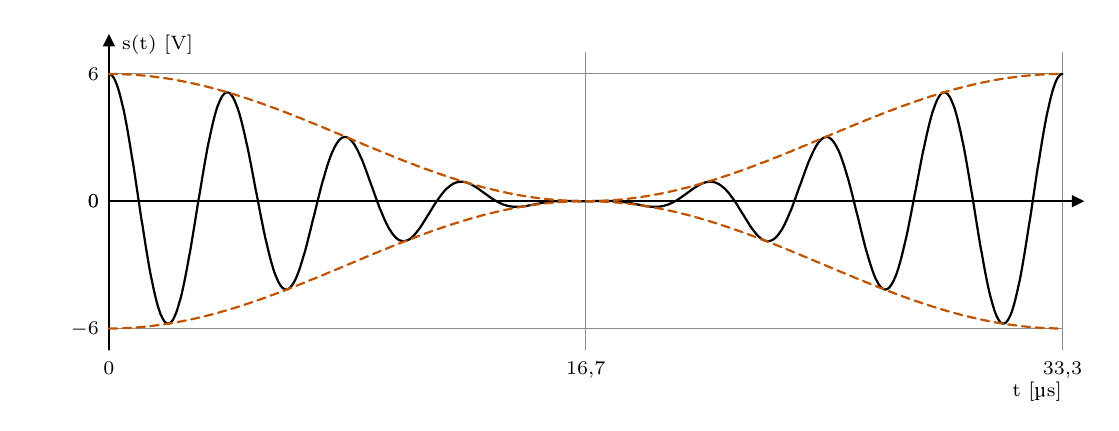
\begin{tikzpicture}[x=0.01985cm,y=-0.01985cm,line cap=round,line join=round]
\useasboundingbox (0,0) rectangle (680,240);
\path[draw=black!45,line width=0.35pt] (52,206) -- (52,16);
\path[draw=black!45,line width=0.35pt] (357,206) -- (357,16);
\path[draw=black!45,line width=0.35pt] (662,206) -- (662,16);
\path[draw=black!45,line width=0.35pt] (52,29.6) -- (662,29.6);
\path[draw=black!45,line width=0.35pt] (52,111) -- (662,111);
\path[draw=black!45,line width=0.35pt] (52,111) -- (662,111);
\path[draw=black!45,line width=0.35pt] (52,192.4) -- (662,192.4);
\path[draw=black,line width=0.7pt] (52,111) -- (670,111);
\path[fill=black,draw=none] (676,111) -- (668,107) -- (668,115) -- cycle;
\path[draw=black,line width=0.7pt] (52,206) -- (52,10);
\path[fill=black,draw=none] (52,4) -- (48,12) -- (56,12) -- cycle;
\node[anchor=base,inner sep=0pt,font=\scriptsize] at (52,222) {0};
\node[anchor=base,inner sep=0pt,font=\scriptsize] at (357,222) {16,7};
\node[anchor=base,inner sep=0pt,font=\scriptsize] at (662,222) {33,3};
\node[anchor=base east,inner sep=0pt,font=\scriptsize] at (46,33.6) {6};
\node[anchor=base east,inner sep=0pt,font=\scriptsize] at (46,115) {0};
\node[anchor=base east,inner sep=0pt,font=\scriptsize] at (46,115) {0};
\node[anchor=base east,inner sep=0pt,font=\scriptsize] at (46,196.4) {$-$6};
\node[anchor=base east,inner sep=0pt,font=\scriptsize] at (662,236) {t [\textmu{}s]};
\node[anchor=base west,inner sep=0pt,font=\scriptsize] at (60,14) {s(t) [V]};
\path[draw=black,line width=0.8pt] (52,29.6) -- (52.5,29.6) -- (53,29.9) -- (53.5,30.2) -- (54,30.7) -- (54.5,31.4) -- (55.1,32.1) -- (55.6,33.1) -- (56.1,34.1) -- (56.6,35.3) -- (57.1,36.7) -- (57.6,38.1) -- (58.1,39.7) -- (58.6,41.4) -- (59.1,43.3) -- (59.6,45.2) -- (60.1,47.3) -- (60.6,49.5) -- (61.2,51.8) -- (61.7,54.2) -- (62.2,56.7) -- (62.7,59.3) -- (63.2,61.9) -- (63.7,64.7) -- (64.2,67.5) -- (64.7,70.5) -- (65.2,73.4) -- (65.7,76.5) -- (66.2,79.6) -- (66.7,82.8) -- (67.3,86) -- (67.8,89.2) -- (68.3,92.5) -- (68.8,95.9) -- (69.3,99.2) -- (69.8,102.6) -- (70.3,105.9) -- (70.8,109.3) -- (71.3,112.7) -- (71.8,116.1) -- (72.3,119.4) -- (72.8,122.8) -- (73.4,126.1) -- (73.9,129.4) -- (74.4,132.6) -- (74.9,135.8) -- (75.4,139) -- (75.9,142.1) -- (76.4,145.1) -- (76.9,148.1) -- (77.4,151) -- (77.9,153.9) -- (78.4,156.6) -- (78.9,159.3) -- (79.5,161.9) -- (80,164.4) -- (80.5,166.8) -- (81,169) -- (81.5,171.2) -- (82,173.3) -- (82.5,175.3) -- (83,177.1) -- (83.5,178.8) -- (84,180.4) -- (84.5,181.9) -- (85,183.3) -- (85.6,184.5) -- (86.1,185.6) -- (86.6,186.5) -- (87.1,187.3) -- (87.6,188) -- (88.1,188.5) -- (88.6,188.9) -- (89.1,189.2) -- (89.6,189.3) -- (90.1,189.3) -- (90.6,189.2) -- (91.1,188.9) -- (91.6,188.5) -- (92.2,187.9) -- (92.7,187.2) -- (93.2,186.4) -- (93.7,185.4) -- (94.2,184.3) -- (94.7,183.1) -- (95.2,181.8) -- (95.7,180.3) -- (96.2,178.7) -- (96.7,177) -- (97.2,175.2) -- (97.8,173.3) -- (98.3,171.3) -- (98.8,169.1) -- (99.3,166.9) -- (99.8,164.6) -- (100.3,162.2) -- (100.8,159.7) -- (101.3,157.1) -- (101.8,154.5) -- (102.3,151.8) -- (102.8,149) -- (103.3,146.1) -- (103.9,143.3) -- (104.4,140.3) -- (104.9,137.3) -- (105.4,134.3) -- (105.9,131.3) -- (106.4,128.2) -- (106.9,125.1) -- (107.4,122) -- (107.9,118.8) -- (108.4,115.7) -- (108.9,112.6) -- (109.4,109.4) -- (110,106.3) -- (110.5,103.2) -- (111,100.2) -- (111.5,97.1) -- (112,94.1) -- (112.5,91.2) -- (113,88.2) -- (113.5,85.4) -- (114,82.6) -- (114.5,79.8) -- (115,77.1) -- (115.5,74.5) -- (116.1,71.9) -- (116.6,69.5) -- (117.1,67.1) -- (117.6,64.8) -- (118.1,62.6) -- (118.6,60.5) -- (119.1,58.5) -- (119.6,56.5) -- (120.1,54.7) -- (120.6,53) -- (121.1,51.4) -- (121.6,49.9) -- (122.2,48.6) -- (122.7,47.3) -- (123.2,46.2) -- (123.7,45.1) -- (124.2,44.2) -- (124.7,43.5) -- (125.2,42.8) -- (125.7,42.3) -- (126.2,41.9) -- (126.7,41.6) -- (127.2,41.4) -- (127.7,41.4) -- (128.3,41.5) -- (128.8,41.7) -- (129.3,42) -- (129.8,42.5) -- (130.3,43.1) -- (130.8,43.8) -- (131.3,44.6) -- (131.8,45.5) -- (132.3,46.5) -- (132.8,47.7) -- (133.3,48.9) -- (133.8,50.3) -- (134.4,51.7) -- (134.9,53.3) -- (135.4,54.9) -- (135.9,56.7) -- (136.4,58.5) -- (136.9,60.4) -- (137.4,62.4) -- (137.9,64.5) -- (138.4,66.6) -- (138.9,68.8) -- (139.4,71.1) -- (139.9,73.4) -- (140.5,75.8) -- (141,78.3) -- (141.5,80.7) -- (142,83.3) -- (142.5,85.8) -- (143,88.4) -- (143.5,91) -- (144,93.7) -- (144.5,96.3) -- (145,99) -- (145.5,101.7) -- (146,104.3) -- (146.6,107) -- (147.1,109.7) -- (147.6,112.3) -- (148.1,115) -- (148.6,117.6) -- (149.1,120.2) -- (149.6,122.7) -- (150.1,125.2) -- (150.6,127.7) -- (151.1,130.2) -- (151.6,132.5) -- (152.1,134.9) -- (152.7,137.2) -- (153.2,139.4) -- (153.7,141.5) -- (154.2,143.6) -- (154.7,145.6) -- (155.2,147.6) -- (155.7,149.5) -- (156.2,151.2) -- (156.7,152.9) -- (157.2,154.6) -- (157.7,156.1) -- (158.2,157.5) -- (158.8,158.9) -- (159.3,160.1) -- (159.8,161.3) -- (160.3,162.4) -- (160.8,163.3) -- (161.3,164.2) -- (161.8,165) -- (162.3,165.6) -- (162.8,166.2) -- (163.3,166.7) -- (163.8,167) -- (164.3,167.3) -- (164.9,167.4) -- (165.4,167.5) -- (165.9,167.4) -- (166.4,167.3) -- (166.9,167) -- (167.4,166.7) -- (167.9,166.3) -- (168.4,165.7) -- (168.9,165.1) -- (169.4,164.4) -- (169.9,163.6) -- (170.4,162.7) -- (171,161.7) -- (171.5,160.6) -- (172,159.5) -- (172.5,158.2) -- (173,156.9) -- (173.5,155.6) -- (174,154.1) -- (174.5,152.6) -- (175,151) -- (175.5,149.4) -- (176,147.7) -- (176.5,146) -- (177.1,144.2) -- (177.6,142.4) -- (178.1,140.5) -- (178.6,138.6) -- (179.1,136.6) -- (179.6,134.6) -- (180.1,132.6) -- (180.6,130.6) -- (181.1,128.6) -- (181.6,126.5) -- (182.1,124.4) -- (182.6,122.4) -- (183.2,120.3) -- (183.7,118.2) -- (184.2,116.1) -- (184.7,114.1) -- (185.2,112) -- (185.7,110) -- (186.2,108) -- (186.7,106) -- (187.2,104) -- (187.7,102.1) -- (188.2,100.2) -- (188.7,98.3) -- (189.3,96.5) -- (189.8,94.7) -- (190.3,92.9) -- (190.8,91.2) -- (191.3,89.6) -- (191.8,88) -- (192.3,86.4) -- (192.8,85) -- (193.3,83.6) -- (193.8,82.2) -- (194.3,80.9) -- (194.8,79.7) -- (195.4,78.5) -- (195.9,77.4) -- (196.4,76.4) -- (196.9,75.5) -- (197.4,74.6) -- (197.9,73.8) -- (198.4,73.1) -- (198.9,72.4) -- (199.4,71.9) -- (199.9,71.4) -- (200.4,70.9) -- (200.9,70.6) -- (201.5,70.3) -- (202,70.1) -- (202.5,70) -- (203,70) -- (203.5,70) -- (204,70.1) -- (204.5,70.3) -- (205,70.5) -- (205.5,70.9) -- (206,71.2) -- (206.5,71.7) -- (207,72.2) -- (207.6,72.8) -- (208.1,73.5) -- (208.6,74.2) -- (209.1,74.9) -- (209.6,75.8) -- (210.1,76.6) -- (210.6,77.6) -- (211.1,78.5) -- (211.6,79.6) -- (212.1,80.6) -- (212.6,81.8) -- (213.1,82.9) -- (213.7,84.1) -- (214.2,85.3) -- (214.7,86.6) -- (215.2,87.9) -- (215.7,89.2) -- (216.2,90.6) -- (216.7,91.9) -- (217.2,93.3) -- (217.7,94.7) -- (218.2,96.1) -- (218.7,97.5) -- (219.2,99) -- (219.7,100.4) -- (220.3,101.8) -- (220.8,103.3) -- (221.3,104.7) -- (221.8,106.1) -- (222.3,107.5) -- (222.8,108.9) -- (223.3,110.3) -- (223.8,111.7) -- (224.3,113) -- (224.8,114.4) -- (225.3,115.7) -- (225.9,117) -- (226.4,118.2) -- (226.9,119.4) -- (227.4,120.6) -- (227.9,121.8) -- (228.4,122.9) -- (228.9,124) -- (229.4,125.1) -- (229.9,126.1) -- (230.4,127.1) -- (230.9,128) -- (231.4,128.9) -- (232,129.7) -- (232.5,130.5) -- (233,131.3) -- (233.5,132) -- (234,132.6) -- (234.5,133.2) -- (235,133.8) -- (235.5,134.3) -- (236,134.7) -- (236.5,135.1) -- (237,135.5) -- (237.5,135.8) -- (238,136) -- (238.6,136.2) -- (239.1,136.4) -- (239.6,136.5) -- (240.1,136.6) -- (240.6,136.6) -- (241.1,136.5) -- (241.6,136.4) -- (242.1,136.3) -- (242.6,136.1) -- (243.1,135.9) -- (243.6,135.7) -- (244.2,135.4) -- (244.7,135) -- (245.2,134.6) -- (245.7,134.2) -- (246.2,133.8) -- (246.7,133.3) -- (247.2,132.7) -- (247.7,132.2) -- (248.2,131.6) -- (248.7,131) -- (249.2,130.3) -- (249.7,129.7) -- (250.3,129) -- (250.8,128.3) -- (251.3,127.5) -- (251.8,126.8) -- (252.3,126) -- (252.8,125.2) -- (253.3,124.4) -- (253.8,123.6) -- (254.3,122.8) -- (254.8,122) -- (255.3,121.2) -- (255.8,120.3) -- (256.4,119.5) -- (256.9,118.7) -- (257.4,117.8) -- (257.9,117) -- (258.4,116.2) -- (258.9,115.4) -- (259.4,114.5) -- (259.9,113.7) -- (260.4,112.9) -- (260.9,112.2) -- (261.4,111.4) -- (261.9,110.6) -- (262.5,109.9) -- (263,109.2) -- (263.5,108.4) -- (264,107.8) -- (264.5,107.1) -- (265,106.4) -- (265.5,105.8) -- (266,105.2) -- (266.5,104.6) -- (267,104.1) -- (267.5,103.5) -- (268,103) -- (268.6,102.6) -- (269.1,102.1) -- (269.6,101.7) -- (270.1,101.3) -- (270.6,100.9) -- (271.1,100.6) -- (271.6,100.2) -- (272.1,99.9) -- (272.6,99.7) -- (273.1,99.5) -- (273.6,99.2) -- (274.1,99.1) -- (274.7,98.9) -- (275.2,98.8) -- (275.7,98.7) -- (276.2,98.6) -- (276.7,98.6) -- (277.2,98.6) -- (277.7,98.6) -- (278.2,98.6) -- (278.7,98.6) -- (279.2,98.7) -- (279.7,98.8) -- (280.2,98.9) -- (280.8,99.1) -- (281.3,99.2) -- (281.8,99.4) -- (282.3,99.6) -- (282.8,99.8) -- (283.3,100.1) -- (283.8,100.3) -- (284.3,100.6) -- (284.8,100.9) -- (285.3,101.1) -- (285.8,101.4) -- (286.3,101.8) -- (286.9,102.1) -- (287.4,102.4) -- (287.9,102.8) -- (288.4,103.1) -- (288.9,103.5) -- (289.4,103.8) -- (289.9,104.2) -- (290.4,104.6) -- (290.9,104.9) -- (291.4,105.3) -- (291.9,105.7) -- (292.4,106) -- (293,106.4) -- (293.5,106.8) -- (294,107.2) -- (294.5,107.5) -- (295,107.9) -- (295.5,108.2) -- (296,108.6) -- (296.5,108.9) -- (297,109.3) -- (297.5,109.6) -- (298,109.9) -- (298.5,110.3) -- (299.1,110.6) -- (299.6,110.9) -- (300.1,111.1) -- (300.6,111.4) -- (301.1,111.7) -- (301.6,111.9) -- (302.1,112.2) -- (302.6,112.4) -- (303.1,112.6) -- (303.6,112.9) -- (304.1,113.1) -- (304.6,113.2) -- (305.2,113.4) -- (305.7,113.6) -- (306.2,113.7) -- (306.7,113.9) -- (307.2,114) -- (307.7,114.1) -- (308.2,114.2) -- (308.7,114.3) -- (309.2,114.4) -- (309.7,114.4) -- (310.2,114.5) -- (310.7,114.6) -- (311.2,114.6) -- (311.8,114.6) -- (312.3,114.6) -- (312.8,114.6) -- (313.3,114.6) -- (313.8,114.6) -- (314.3,114.6) -- (314.8,114.6) -- (315.3,114.5) -- (315.8,114.5) -- (316.3,114.4) -- (316.8,114.4) -- (317.3,114.3) -- (317.9,114.3) -- (318.4,114.2) -- (318.9,114.1) -- (319.4,114) -- (319.9,113.9) -- (320.4,113.8) -- (320.9,113.7) -- (321.4,113.6) -- (321.9,113.5) -- (322.4,113.4) -- (322.9,113.3) -- (323.5,113.2) -- (324,113.1) -- (324.5,113) -- (325,112.9) -- (325.5,112.8) -- (326,112.7) -- (326.5,112.6) -- (327,112.5) -- (327.5,112.4) -- (328,112.3) -- (328.5,112.2) -- (329,112.1) -- (329.5,112) -- (330.1,111.9) -- (330.6,111.9) -- (331.1,111.8) -- (331.6,111.7) -- (332.1,111.6) -- (332.6,111.5) -- (333.1,111.5) -- (333.6,111.4) -- (334.1,111.3) -- (334.6,111.3) -- (335.1,111.2) -- (335.7,111.2) -- (336.2,111.1) -- (336.7,111.1) -- (337.2,111.1) -- (337.7,111) -- (338.2,111) -- (338.7,111) -- (339.2,110.9) -- (339.7,110.9) -- (340.2,110.9) -- (340.7,110.9) -- (341.2,110.9) -- (341.8,110.8) -- (342.3,110.8) -- (342.8,110.8) -- (343.3,110.8) -- (343.8,110.8) -- (344.3,110.8) -- (344.8,110.8) -- (345.3,110.8) -- (345.8,110.8) -- (346.3,110.8) -- (346.8,110.9) -- (347.3,110.9) -- (347.8,110.9) -- (348.4,110.9) -- (348.9,110.9) -- (349.4,110.9) -- (349.9,110.9) -- (350.4,110.9) -- (350.9,110.9) -- (351.4,110.9) -- (351.9,110.9) -- (352.4,111) -- (352.9,111) -- (353.4,111) -- (354,111) -- (354.5,111) -- (355,111) -- (355.5,111) -- (356,111) -- (356.5,111) -- (357,111) -- (357.5,111) -- (358,111) -- (358.5,111) -- (359,111) -- (359.5,111) -- (360,111) -- (360.6,111) -- (361.1,111) -- (361.6,111) -- (362.1,110.9) -- (362.6,110.9) -- (363.1,110.9) -- (363.6,110.9) -- (364.1,110.9) -- (364.6,110.9) -- (365.1,110.9) -- (365.6,110.9) -- (366.2,110.9) -- (366.7,110.9) -- (367.2,110.9) -- (367.7,110.8) -- (368.2,110.8) -- (368.7,110.8) -- (369.2,110.8) -- (369.7,110.8) -- (370.2,110.8) -- (370.7,110.8) -- (371.2,110.8) -- (371.7,110.8) -- (372.2,110.8) -- (372.8,110.9) -- (373.3,110.9) -- (373.8,110.9) -- (374.3,110.9) -- (374.8,110.9) -- (375.3,111) -- (375.8,111) -- (376.3,111) -- (376.8,111.1) -- (377.3,111.1) -- (377.8,111.1) -- (378.3,111.2) -- (378.9,111.2) -- (379.4,111.3) -- (379.9,111.3) -- (380.4,111.4) -- (380.9,111.5) -- (381.4,111.5) -- (381.9,111.6) -- (382.4,111.7) -- (382.9,111.8) -- (383.4,111.9) -- (383.9,111.9) -- (384.5,112) -- (385,112.1) -- (385.5,112.2) -- (386,112.3) -- (386.5,112.4) -- (387,112.5) -- (387.5,112.6) -- (388,112.7) -- (388.5,112.8) -- (389,112.9) -- (389.5,113) -- (390,113.1) -- (390.5,113.2) -- (391.1,113.3) -- (391.6,113.4) -- (392.1,113.5) -- (392.6,113.6) -- (393.1,113.7) -- (393.6,113.8) -- (394.1,113.9) -- (394.6,114) -- (395.1,114.1) -- (395.6,114.2) -- (396.1,114.3) -- (396.7,114.3) -- (397.2,114.4) -- (397.7,114.4) -- (398.2,114.5) -- (398.7,114.5) -- (399.2,114.6) -- (399.7,114.6) -- (400.2,114.6) -- (400.7,114.6) -- (401.2,114.6) -- (401.7,114.6) -- (402.2,114.6) -- (402.8,114.6) -- (403.3,114.6) -- (403.8,114.5) -- (404.3,114.4) -- (404.8,114.4) -- (405.3,114.3) -- (405.8,114.2) -- (406.3,114.1) -- (406.8,114) -- (407.3,113.9) -- (407.8,113.7) -- (408.3,113.6) -- (408.8,113.4) -- (409.4,113.2) -- (409.9,113.1) -- (410.4,112.9) -- (410.9,112.6) -- (411.4,112.4) -- (411.9,112.2) -- (412.4,111.9) -- (412.9,111.7) -- (413.4,111.4) -- (413.9,111.1) -- (414.4,110.9) -- (415,110.6) -- (415.5,110.3) -- (416,109.9) -- (416.5,109.6) -- (417,109.3) -- (417.5,108.9) -- (418,108.6) -- (418.5,108.2) -- (419,107.9) -- (419.5,107.5) -- (420,107.2) -- (420.5,106.8) -- (421.1,106.4) -- (421.6,106) -- (422.1,105.7) -- (422.6,105.3) -- (423.1,104.9) -- (423.6,104.6) -- (424.1,104.2) -- (424.6,103.8) -- (425.1,103.5) -- (425.6,103.1) -- (426.1,102.8) -- (426.6,102.4) -- (427.2,102.1) -- (427.7,101.8) -- (428.2,101.4) -- (428.7,101.1) -- (429.2,100.9) -- (429.7,100.6) -- (430.2,100.3) -- (430.7,100.1) -- (431.2,99.8) -- (431.7,99.6) -- (432.2,99.4) -- (432.7,99.2) -- (433.2,99.1) -- (433.8,98.9) -- (434.3,98.8) -- (434.8,98.7) -- (435.3,98.6) -- (435.8,98.6) -- (436.3,98.6) -- (436.8,98.6) -- (437.3,98.6) -- (437.8,98.6) -- (438.3,98.7) -- (438.8,98.8) -- (439.4,98.9) -- (439.9,99.1) -- (440.4,99.2) -- (440.9,99.5) -- (441.4,99.7) -- (441.9,99.9) -- (442.4,100.2) -- (442.9,100.6) -- (443.4,100.9) -- (443.9,101.3) -- (444.4,101.7) -- (444.9,102.1) -- (445.5,102.6) -- (446,103) -- (446.5,103.5) -- (447,104.1) -- (447.5,104.6) -- (448,105.2) -- (448.5,105.8) -- (449,106.4) -- (449.5,107.1) -- (450,107.8) -- (450.5,108.4) -- (451,109.2) -- (451.6,109.9) -- (452.1,110.6) -- (452.6,111.4) -- (453.1,112.2) -- (453.6,112.9) -- (454.1,113.7) -- (454.6,114.5) -- (455.1,115.4) -- (455.6,116.2) -- (456.1,117) -- (456.6,117.8) -- (457.1,118.7) -- (457.7,119.5) -- (458.2,120.3) -- (458.7,121.2) -- (459.2,122) -- (459.7,122.8) -- (460.2,123.6) -- (460.7,124.4) -- (461.2,125.2) -- (461.7,126) -- (462.2,126.8) -- (462.7,127.5) -- (463.2,128.3) -- (463.8,129) -- (464.3,129.7) -- (464.8,130.3) -- (465.3,131) -- (465.8,131.6) -- (466.3,132.2) -- (466.8,132.7) -- (467.3,133.3) -- (467.8,133.8) -- (468.3,134.2) -- (468.8,134.6) -- (469.3,135) -- (469.9,135.4) -- (470.4,135.7) -- (470.9,135.9) -- (471.4,136.1) -- (471.9,136.3) -- (472.4,136.4) -- (472.9,136.5) -- (473.4,136.6) -- (473.9,136.6) -- (474.4,136.5) -- (474.9,136.4) -- (475.4,136.2) -- (476,136) -- (476.5,135.8) -- (477,135.5) -- (477.5,135.1) -- (478,134.7) -- (478.5,134.3) -- (479,133.8) -- (479.5,133.2) -- (480,132.6) -- (480.5,132) -- (481,131.3) -- (481.5,130.5) -- (482.1,129.7) -- (482.6,128.9) -- (483.1,128) -- (483.6,127.1) -- (484.1,126.1) -- (484.6,125.1) -- (485.1,124) -- (485.6,122.9) -- (486.1,121.8) -- (486.6,120.6) -- (487.1,119.4) -- (487.6,118.2) -- (488.2,117) -- (488.7,115.7) -- (489.2,114.4) -- (489.7,113) -- (490.2,111.7) -- (490.7,110.3) -- (491.2,108.9) -- (491.7,107.5) -- (492.2,106.1) -- (492.7,104.7) -- (493.2,103.3) -- (493.7,101.8) -- (494.3,100.4) -- (494.8,99) -- (495.3,97.5) -- (495.8,96.1) -- (496.3,94.7) -- (496.8,93.3) -- (497.3,91.9) -- (497.8,90.6) -- (498.3,89.2) -- (498.8,87.9) -- (499.3,86.6) -- (499.8,85.3) -- (500.4,84.1) -- (500.9,82.9) -- (501.4,81.8) -- (501.9,80.6) -- (502.4,79.6) -- (502.9,78.5) -- (503.4,77.6) -- (503.9,76.6) -- (504.4,75.8) -- (504.9,74.9) -- (505.4,74.2) -- (505.9,73.5) -- (506.5,72.8) -- (507,72.2) -- (507.5,71.7) -- (508,71.2) -- (508.5,70.9) -- (509,70.5) -- (509.5,70.3) -- (510,70.1) -- (510.5,70) -- (511,70) -- (511.5,70) -- (512,70.1) -- (512.6,70.3) -- (513.1,70.6) -- (513.6,70.9) -- (514.1,71.4) -- (514.6,71.9) -- (515.1,72.4) -- (515.6,73.1) -- (516.1,73.8) -- (516.6,74.6) -- (517.1,75.5) -- (517.6,76.4) -- (518.1,77.4) -- (518.7,78.5) -- (519.2,79.7) -- (519.7,80.9) -- (520.2,82.2) -- (520.7,83.6) -- (521.2,85) -- (521.7,86.4) -- (522.2,88) -- (522.7,89.6) -- (523.2,91.2) -- (523.7,92.9) -- (524.2,94.7) -- (524.8,96.5) -- (525.3,98.3) -- (525.8,100.2) -- (526.3,102.1) -- (526.8,104) -- (527.3,106) -- (527.8,108) -- (528.3,110) -- (528.8,112) -- (529.3,114.1) -- (529.8,116.1) -- (530.3,118.2) -- (530.9,120.3) -- (531.4,122.4) -- (531.9,124.4) -- (532.4,126.5) -- (532.9,128.6) -- (533.4,130.6) -- (533.9,132.6) -- (534.4,134.6) -- (534.9,136.6) -- (535.4,138.6) -- (535.9,140.5) -- (536.4,142.4) -- (537,144.2) -- (537.5,146) -- (538,147.7) -- (538.5,149.4) -- (539,151) -- (539.5,152.6) -- (540,154.1) -- (540.5,155.6) -- (541,156.9) -- (541.5,158.2) -- (542,159.5) -- (542.5,160.6) -- (543.1,161.7) -- (543.6,162.7) -- (544.1,163.6) -- (544.6,164.4) -- (545.1,165.1) -- (545.6,165.7) -- (546.1,166.3) -- (546.6,166.7) -- (547.1,167) -- (547.6,167.3) -- (548.1,167.4) -- (548.6,167.5) -- (549.2,167.4) -- (549.7,167.3) -- (550.2,167) -- (550.7,166.7) -- (551.2,166.2) -- (551.7,165.6) -- (552.2,165) -- (552.7,164.2) -- (553.2,163.3) -- (553.7,162.4) -- (554.2,161.3) -- (554.7,160.1) -- (555.3,158.9) -- (555.8,157.5) -- (556.3,156.1) -- (556.8,154.6) -- (557.3,152.9) -- (557.8,151.2) -- (558.3,149.5) -- (558.8,147.6) -- (559.3,145.6) -- (559.8,143.6) -- (560.3,141.5) -- (560.8,139.4) -- (561.3,137.2) -- (561.9,134.9) -- (562.4,132.5) -- (562.9,130.2) -- (563.4,127.7) -- (563.9,125.2) -- (564.4,122.7) -- (564.9,120.2) -- (565.4,117.6) -- (565.9,115) -- (566.4,112.3) -- (566.9,109.7) -- (567.4,107) -- (568,104.3) -- (568.5,101.7) -- (569,99) -- (569.5,96.3) -- (570,93.7) -- (570.5,91) -- (571,88.4) -- (571.5,85.8) -- (572,83.3) -- (572.5,80.7) -- (573,78.3) -- (573.6,75.8) -- (574.1,73.4) -- (574.6,71.1) -- (575.1,68.8) -- (575.6,66.6) -- (576.1,64.5) -- (576.6,62.4) -- (577.1,60.4) -- (577.6,58.5) -- (578.1,56.7) -- (578.6,54.9) -- (579.1,53.3) -- (579.7,51.7) -- (580.2,50.3) -- (580.7,48.9) -- (581.2,47.7) -- (581.7,46.5) -- (582.2,45.5) -- (582.7,44.6) -- (583.2,43.8) -- (583.7,43.1) -- (584.2,42.5) -- (584.7,42) -- (585.2,41.7) -- (585.8,41.5) -- (586.3,41.4) -- (586.8,41.4) -- (587.3,41.6) -- (587.8,41.9) -- (588.3,42.3) -- (588.8,42.8) -- (589.3,43.5) -- (589.8,44.2) -- (590.3,45.1) -- (590.8,46.2) -- (591.3,47.3) -- (591.8,48.6) -- (592.4,49.9) -- (592.9,51.4) -- (593.4,53) -- (593.9,54.7) -- (594.4,56.5) -- (594.9,58.5) -- (595.4,60.5) -- (595.9,62.6) -- (596.4,64.8) -- (596.9,67.1) -- (597.4,69.5) -- (597.9,71.9) -- (598.5,74.5) -- (599,77.1) -- (599.5,79.8) -- (600,82.6) -- (600.5,85.4) -- (601,88.2) -- (601.5,91.2) -- (602,94.1) -- (602.5,97.1) -- (603,100.2) -- (603.5,103.2) -- (604.1,106.3) -- (604.6,109.4) -- (605.1,112.6) -- (605.6,115.7) -- (606.1,118.8) -- (606.6,122) -- (607.1,125.1) -- (607.6,128.2) -- (608.1,131.3) -- (608.6,134.3) -- (609.1,137.3) -- (609.6,140.3) -- (610.2,143.3) -- (610.7,146.1) -- (611.2,149) -- (611.7,151.8) -- (612.2,154.5) -- (612.7,157.1) -- (613.2,159.7) -- (613.7,162.2) -- (614.2,164.6) -- (614.7,166.9) -- (615.2,169.1) -- (615.7,171.3) -- (616.3,173.3) -- (616.8,175.2) -- (617.3,177) -- (617.8,178.7) -- (618.3,180.3) -- (618.8,181.8) -- (619.3,183.1) -- (619.8,184.3) -- (620.3,185.4) -- (620.8,186.4) -- (621.3,187.2) -- (621.8,187.9) -- (622.3,188.5) -- (622.9,188.9) -- (623.4,189.2) -- (623.9,189.3) -- (624.4,189.3) -- (624.9,189.2) -- (625.4,188.9) -- (625.9,188.5) -- (626.4,188) -- (626.9,187.3) -- (627.4,186.5) -- (627.9,185.6) -- (628.4,184.5) -- (629,183.3) -- (629.5,181.9) -- (630,180.4) -- (630.5,178.8) -- (631,177.1) -- (631.5,175.3) -- (632,173.3) -- (632.5,171.2) -- (633,169) -- (633.5,166.8) -- (634,164.4) -- (634.6,161.9) -- (635.1,159.3) -- (635.6,156.6) -- (636.1,153.9) -- (636.6,151) -- (637.1,148.1) -- (637.6,145.1) -- (638.1,142.1) -- (638.6,139) -- (639.1,135.8) -- (639.6,132.6) -- (640.1,129.4) -- (640.6,126.1) -- (641.2,122.8) -- (641.7,119.4) -- (642.2,116.1) -- (642.7,112.7) -- (643.2,109.3) -- (643.7,105.9) -- (644.2,102.6) -- (644.7,99.2) -- (645.2,95.9) -- (645.7,92.5) -- (646.2,89.2) -- (646.8,86) -- (647.3,82.8) -- (647.8,79.6) -- (648.3,76.5) -- (648.8,73.4) -- (649.3,70.5) -- (649.8,67.5) -- (650.3,64.7) -- (650.8,61.9) -- (651.3,59.3) -- (651.8,56.7) -- (652.3,54.2) -- (652.9,51.8) -- (653.4,49.5) -- (653.9,47.3) -- (654.4,45.2) -- (654.9,43.3) -- (655.4,41.4) -- (655.9,39.7) -- (656.4,38.1) -- (656.9,36.7) -- (657.4,35.3) -- (657.9,34.1) -- (658.4,33.1) -- (658.9,32.1) -- (659.5,31.4) -- (660,30.7) -- (660.5,30.2) -- (661,29.9) -- (661.5,29.6) -- (662,29.6);
\path[draw=cB,line width=0.8pt,dash pattern=on 3pt off 2pt] (52,29.6) -- (52.8,29.6) -- (53.5,29.6) -- (54.3,29.6) -- (55.1,29.6) -- (55.8,29.6) -- (56.6,29.6) -- (57.3,29.6) -- (58.1,29.7) -- (58.9,29.7) -- (59.6,29.7) -- (60.4,29.7) -- (61.2,29.8) -- (61.9,29.8) -- (62.7,29.8) -- (63.4,29.9) -- (64.2,29.9) -- (65,29.9) -- (65.7,30) -- (66.5,30) -- (67.3,30.1) -- (68,30.1) -- (68.8,30.2) -- (69.5,30.2) -- (70.3,30.3) -- (71.1,30.4) -- (71.8,30.4) -- (72.6,30.5) -- (73.4,30.6) -- (74.1,30.6) -- (74.9,30.7) -- (75.6,30.8) -- (76.4,30.9) -- (77.2,30.9) -- (77.9,31) -- (78.7,31.1) -- (79.5,31.2) -- (80.2,31.3) -- (81,31.4) -- (81.7,31.5) -- (82.5,31.6) -- (83.3,31.7) -- (84,31.8) -- (84.8,31.9) -- (85.6,32) -- (86.3,32.1) -- (87.1,32.2) -- (87.8,32.3) -- (88.6,32.4) -- (89.4,32.5) -- (90.1,32.7) -- (90.9,32.8) -- (91.7,32.9) -- (92.4,33) -- (93.2,33.2) -- (93.9,33.3) -- (94.7,33.4) -- (95.5,33.6) -- (96.2,33.7) -- (97,33.9) -- (97.8,34) -- (98.5,34.2) -- (99.3,34.3) -- (100,34.5) -- (100.8,34.6) -- (101.6,34.8) -- (102.3,34.9) -- (103.1,35.1) -- (103.9,35.2) -- (104.6,35.4) -- (105.4,35.6) -- (106.1,35.7) -- (106.9,35.9) -- (107.7,36.1) -- (108.4,36.3) -- (109.2,36.4) -- (110,36.6) -- (110.7,36.8) -- (111.5,37) -- (112.2,37.2) -- (113,37.3) -- (113.8,37.5) -- (114.5,37.7) -- (115.3,37.9) -- (116.1,38.1) -- (116.8,38.3) -- (117.6,38.5) -- (118.3,38.7) -- (119.1,38.9) -- (119.9,39.1) -- (120.6,39.3) -- (121.4,39.5) -- (122.2,39.7) -- (122.9,40) -- (123.7,40.2) -- (124.4,40.4) -- (125.2,40.6) -- (126,40.8) -- (126.7,41) -- (127.5,41.3) -- (128.3,41.5) -- (129,41.7) -- (129.8,42) -- (130.5,42.2) -- (131.3,42.4) -- (132.1,42.6) -- (132.8,42.9) -- (133.6,43.1) -- (134.4,43.4) -- (135.1,43.6) -- (135.9,43.8) -- (136.6,44.1) -- (137.4,44.3) -- (138.2,44.6) -- (138.9,44.8) -- (139.7,45.1) -- (140.5,45.3) -- (141.2,45.6) -- (142,45.8) -- (142.7,46.1) -- (143.5,46.4) -- (144.3,46.6) -- (145,46.9) -- (145.8,47.1) -- (146.6,47.4) -- (147.3,47.7) -- (148.1,47.9) -- (148.8,48.2) -- (149.6,48.5) -- (150.4,48.7) -- (151.1,49) -- (151.9,49.3) -- (152.6,49.6) -- (153.4,49.8) -- (154.2,50.1) -- (154.9,50.4) -- (155.7,50.7) -- (156.5,51) -- (157.2,51.2) -- (158,51.5) -- (158.8,51.8) -- (159.5,52.1) -- (160.3,52.4) -- (161,52.7) -- (161.8,53) -- (162.6,53.2) -- (163.3,53.5) -- (164.1,53.8) -- (164.9,54.1) -- (165.6,54.4) -- (166.4,54.7) -- (167.1,55) -- (167.9,55.3) -- (168.7,55.6) -- (169.4,55.9) -- (170.2,56.2) -- (171,56.5) -- (171.7,56.8) -- (172.5,57.1) -- (173.2,57.4) -- (174,57.7) -- (174.8,58) -- (175.5,58.3) -- (176.3,58.6) -- (177.1,58.9) -- (177.8,59.2) -- (178.6,59.5) -- (179.3,59.9) -- (180.1,60.2) -- (180.9,60.5) -- (181.6,60.8) -- (182.4,61.1) -- (183.2,61.4) -- (183.9,61.7) -- (184.7,62) -- (185.4,62.3) -- (186.2,62.7) -- (187,63) -- (187.7,63.3) -- (188.5,63.6) -- (189.3,63.9) -- (190,64.2) -- (190.8,64.5) -- (191.5,64.9) -- (192.3,65.2) -- (193.1,65.5) -- (193.8,65.8) -- (194.6,66.1) -- (195.4,66.5) -- (196.1,66.8) -- (196.9,67.1) -- (197.6,67.4) -- (198.4,67.7) -- (199.2,68) -- (199.9,68.4) -- (200.7,68.7) -- (201.5,69) -- (202.2,69.3) -- (203,69.6) -- (203.7,70) -- (204.5,70.3) -- (205.3,70.6) -- (206,70.9) -- (206.8,71.2) -- (207.6,71.6) -- (208.3,71.9) -- (209.1,72.2) -- (209.8,72.5) -- (210.6,72.8) -- (211.4,73.2) -- (212.1,73.5) -- (212.9,73.8) -- (213.7,74.1) -- (214.4,74.4) -- (215.2,74.8) -- (215.9,75.1) -- (216.7,75.4) -- (217.5,75.7) -- (218.2,76) -- (219,76.3) -- (219.8,76.7) -- (220.5,77) -- (221.3,77.3) -- (222,77.6) -- (222.8,77.9) -- (223.6,78.2) -- (224.3,78.5) -- (225.1,78.9) -- (225.9,79.2) -- (226.6,79.5) -- (227.4,79.8) -- (228.1,80.1) -- (228.9,80.4) -- (229.7,80.7) -- (230.4,81) -- (231.2,81.3) -- (232,81.6) -- (232.7,82) -- (233.5,82.3) -- (234.2,82.6) -- (235,82.9) -- (235.8,83.2) -- (236.5,83.5) -- (237.3,83.8) -- (238.1,84.1) -- (238.8,84.4) -- (239.6,84.7) -- (240.3,85) -- (241.1,85.3) -- (241.9,85.6) -- (242.6,85.9) -- (243.4,86.2) -- (244.2,86.5) -- (244.9,86.7) -- (245.7,87) -- (246.4,87.3) -- (247.2,87.6) -- (248,87.9) -- (248.7,88.2) -- (249.5,88.5) -- (250.3,88.8) -- (251,89.1) -- (251.8,89.3) -- (252.5,89.6) -- (253.3,89.9) -- (254.1,90.2) -- (254.8,90.5) -- (255.6,90.7) -- (256.4,91) -- (257.1,91.3) -- (257.9,91.6) -- (258.6,91.8) -- (259.4,92.1) -- (260.2,92.4) -- (260.9,92.6) -- (261.7,92.9) -- (262.5,93.2) -- (263.2,93.4) -- (264,93.7) -- (264.7,94) -- (265.5,94.2) -- (266.3,94.5) -- (267,94.7) -- (267.8,95) -- (268.6,95.2) -- (269.3,95.5) -- (270.1,95.7) -- (270.8,96) -- (271.6,96.2) -- (272.4,96.5) -- (273.1,96.7) -- (273.9,97) -- (274.7,97.2) -- (275.4,97.4) -- (276.2,97.7) -- (276.9,97.9) -- (277.7,98.2) -- (278.5,98.4) -- (279.2,98.6) -- (280,98.8) -- (280.8,99.1) -- (281.5,99.3) -- (282.3,99.5) -- (283,99.7) -- (283.8,100) -- (284.6,100.2) -- (285.3,100.4) -- (286.1,100.6) -- (286.9,100.8) -- (287.6,101) -- (288.4,101.2) -- (289.1,101.5) -- (289.9,101.7) -- (290.7,101.9) -- (291.4,102.1) -- (292.2,102.3) -- (293,102.5) -- (293.7,102.7) -- (294.5,102.8) -- (295.2,103) -- (296,103.2) -- (296.8,103.4) -- (297.5,103.6) -- (298.3,103.8) -- (299,104) -- (299.8,104.1) -- (300.6,104.3) -- (301.3,104.5) -- (302.1,104.7) -- (302.9,104.8) -- (303.6,105) -- (304.4,105.2) -- (305.2,105.3) -- (305.9,105.5) -- (306.7,105.7) -- (307.4,105.8) -- (308.2,106) -- (309,106.1) -- (309.7,106.3) -- (310.5,106.4) -- (311.3,106.6) -- (312,106.7) -- (312.8,106.8) -- (313.5,107) -- (314.3,107.1) -- (315.1,107.3) -- (315.8,107.4) -- (316.6,107.5) -- (317.3,107.7) -- (318.1,107.8) -- (318.9,107.9) -- (319.6,108) -- (320.4,108.1) -- (321.2,108.3) -- (321.9,108.4) -- (322.7,108.5) -- (323.5,108.6) -- (324.2,108.7) -- (325,108.8) -- (325.7,108.9) -- (326.5,109) -- (327.3,109.1) -- (328,109.2) -- (328.8,109.3) -- (329.6,109.4) -- (330.3,109.5) -- (331.1,109.6) -- (331.8,109.6) -- (332.6,109.7) -- (333.4,109.8) -- (334.1,109.9) -- (334.9,109.9) -- (335.7,110) -- (336.4,110.1) -- (337.2,110.2) -- (337.9,110.2) -- (338.7,110.3) -- (339.5,110.3) -- (340.2,110.4) -- (341,110.4) -- (341.8,110.5) -- (342.5,110.5) -- (343.3,110.6) -- (344,110.6) -- (344.8,110.7) -- (345.6,110.7) -- (346.3,110.8) -- (347.1,110.8) -- (347.8,110.8) -- (348.6,110.8) -- (349.4,110.9) -- (350.1,110.9) -- (350.9,110.9) -- (351.7,110.9) -- (352.4,111) -- (353.2,111) -- (354,111) -- (354.7,111) -- (355.5,111) -- (356.2,111) -- (357,111) -- (357.8,111) -- (358.5,111) -- (359.3,111) -- (360.1,111) -- (360.8,111) -- (361.6,111) -- (362.3,110.9) -- (363.1,110.9) -- (363.9,110.9) -- (364.6,110.9) -- (365.4,110.8) -- (366.2,110.8) -- (366.9,110.8) -- (367.7,110.8) -- (368.4,110.7) -- (369.2,110.7) -- (370,110.6) -- (370.7,110.6) -- (371.5,110.5) -- (372.3,110.5) -- (373,110.4) -- (373.8,110.4) -- (374.5,110.3) -- (375.3,110.3) -- (376.1,110.2) -- (376.8,110.2) -- (377.6,110.1) -- (378.4,110) -- (379.1,109.9) -- (379.9,109.9) -- (380.6,109.8) -- (381.4,109.7) -- (382.2,109.6) -- (382.9,109.6) -- (383.7,109.5) -- (384.5,109.4) -- (385.2,109.3) -- (386,109.2) -- (386.7,109.1) -- (387.5,109) -- (388.3,108.9) -- (389,108.8) -- (389.8,108.7) -- (390.6,108.6) -- (391.3,108.5) -- (392.1,108.4) -- (392.8,108.3) -- (393.6,108.1) -- (394.4,108) -- (395.1,107.9) -- (395.9,107.8) -- (396.7,107.7) -- (397.4,107.5) -- (398.2,107.4) -- (398.9,107.3) -- (399.7,107.1) -- (400.5,107) -- (401.2,106.8) -- (402,106.7) -- (402.8,106.6) -- (403.5,106.4) -- (404.3,106.3) -- (405,106.1) -- (405.8,106) -- (406.6,105.8) -- (407.3,105.7) -- (408.1,105.5) -- (408.9,105.3) -- (409.6,105.2) -- (410.4,105) -- (411.1,104.8) -- (411.9,104.7) -- (412.7,104.5) -- (413.4,104.3) -- (414.2,104.1) -- (415,104) -- (415.7,103.8) -- (416.5,103.6) -- (417.2,103.4) -- (418,103.2) -- (418.8,103) -- (419.5,102.8) -- (420.3,102.7) -- (421.1,102.5) -- (421.8,102.3) -- (422.6,102.1) -- (423.3,101.9) -- (424.1,101.7) -- (424.9,101.5) -- (425.6,101.2) -- (426.4,101) -- (427.2,100.8) -- (427.9,100.6) -- (428.7,100.4) -- (429.4,100.2) -- (430.2,100) -- (431,99.7) -- (431.7,99.5) -- (432.5,99.3) -- (433.3,99.1) -- (434,98.8) -- (434.8,98.6) -- (435.5,98.4) -- (436.3,98.2) -- (437.1,97.9) -- (437.8,97.7) -- (438.6,97.4) -- (439.4,97.2) -- (440.1,97) -- (440.9,96.7) -- (441.6,96.5) -- (442.4,96.2) -- (443.2,96) -- (443.9,95.7) -- (444.7,95.5) -- (445.4,95.2) -- (446.2,95) -- (447,94.7) -- (447.7,94.5) -- (448.5,94.2) -- (449.3,94) -- (450,93.7) -- (450.8,93.4) -- (451.6,93.2) -- (452.3,92.9) -- (453.1,92.6) -- (453.8,92.4) -- (454.6,92.1) -- (455.4,91.8) -- (456.1,91.6) -- (456.9,91.3) -- (457.7,91) -- (458.4,90.7) -- (459.2,90.5) -- (459.9,90.2) -- (460.7,89.9) -- (461.5,89.6) -- (462.2,89.3) -- (463,89.1) -- (463.7,88.8) -- (464.5,88.5) -- (465.3,88.2) -- (466,87.9) -- (466.8,87.6) -- (467.6,87.3) -- (468.3,87) -- (469.1,86.7) -- (469.9,86.5) -- (470.6,86.2) -- (471.4,85.9) -- (472.1,85.6) -- (472.9,85.3) -- (473.7,85) -- (474.4,84.7) -- (475.2,84.4) -- (476,84.1) -- (476.7,83.8) -- (477.5,83.5) -- (478.2,83.2) -- (479,82.9) -- (479.8,82.6) -- (480.5,82.3) -- (481.3,82) -- (482.1,81.6) -- (482.8,81.3) -- (483.6,81) -- (484.3,80.7) -- (485.1,80.4) -- (485.9,80.1) -- (486.6,79.8) -- (487.4,79.5) -- (488.2,79.2) -- (488.9,78.9) -- (489.7,78.5) -- (490.4,78.2) -- (491.2,77.9) -- (492,77.6) -- (492.7,77.3) -- (493.5,77) -- (494.3,76.7) -- (495,76.3) -- (495.8,76) -- (496.5,75.7) -- (497.3,75.4) -- (498.1,75.1) -- (498.8,74.8) -- (499.6,74.4) -- (500.4,74.1) -- (501.1,73.8) -- (501.9,73.5) -- (502.6,73.2) -- (503.4,72.8) -- (504.2,72.5) -- (504.9,72.2) -- (505.7,71.9) -- (506.5,71.6) -- (507.2,71.2) -- (508,70.9) -- (508.7,70.6) -- (509.5,70.3) -- (510.3,70) -- (511,69.6) -- (511.8,69.3) -- (512.6,69) -- (513.3,68.7) -- (514.1,68.4) -- (514.8,68) -- (515.6,67.7) -- (516.4,67.4) -- (517.1,67.1) -- (517.9,66.8) -- (518.6,66.5) -- (519.4,66.1) -- (520.2,65.8) -- (520.9,65.5) -- (521.7,65.2) -- (522.5,64.9) -- (523.2,64.5) -- (524,64.2) -- (524.8,63.9) -- (525.5,63.6) -- (526.3,63.3) -- (527,63) -- (527.8,62.7) -- (528.6,62.3) -- (529.3,62) -- (530.1,61.7) -- (530.9,61.4) -- (531.6,61.1) -- (532.4,60.8) -- (533.1,60.5) -- (533.9,60.2) -- (534.7,59.9) -- (535.4,59.5) -- (536.2,59.2) -- (536.9,58.9) -- (537.7,58.6) -- (538.5,58.3) -- (539.2,58) -- (540,57.7) -- (540.8,57.4) -- (541.5,57.1) -- (542.3,56.8) -- (543.1,56.5) -- (543.8,56.2) -- (544.6,55.9) -- (545.3,55.6) -- (546.1,55.3) -- (546.9,55) -- (547.6,54.7) -- (548.4,54.4) -- (549.2,54.1) -- (549.9,53.8) -- (550.7,53.5) -- (551.4,53.2) -- (552.2,53) -- (553,52.7) -- (553.7,52.4) -- (554.5,52.1) -- (555.3,51.8) -- (556,51.5) -- (556.8,51.2) -- (557.5,51) -- (558.3,50.7) -- (559.1,50.4) -- (559.8,50.1) -- (560.6,49.8) -- (561.3,49.6) -- (562.1,49.3) -- (562.9,49) -- (563.6,48.7) -- (564.4,48.5) -- (565.2,48.2) -- (565.9,47.9) -- (566.7,47.7) -- (567.5,47.4) -- (568.2,47.1) -- (569,46.9) -- (569.7,46.6) -- (570.5,46.4) -- (571.3,46.1) -- (572,45.8) -- (572.8,45.6) -- (573.6,45.3) -- (574.3,45.1) -- (575.1,44.8) -- (575.8,44.6) -- (576.6,44.3) -- (577.4,44.1) -- (578.1,43.8) -- (578.9,43.6) -- (579.7,43.4) -- (580.4,43.1) -- (581.2,42.9) -- (581.9,42.6) -- (582.7,42.4) -- (583.5,42.2) -- (584.2,42) -- (585,41.7) -- (585.8,41.5) -- (586.5,41.3) -- (587.3,41) -- (588,40.8) -- (588.8,40.6) -- (589.6,40.4) -- (590.3,40.2) -- (591.1,40) -- (591.8,39.7) -- (592.6,39.5) -- (593.4,39.3) -- (594.1,39.1) -- (594.9,38.9) -- (595.7,38.7) -- (596.4,38.5) -- (597.2,38.3) -- (598,38.1) -- (598.7,37.9) -- (599.5,37.7) -- (600.2,37.5) -- (601,37.3) -- (601.8,37.2) -- (602.5,37) -- (603.3,36.8) -- (604.1,36.6) -- (604.8,36.4) -- (605.6,36.3) -- (606.3,36.1) -- (607.1,35.9) -- (607.9,35.7) -- (608.6,35.6) -- (609.4,35.4) -- (610.2,35.2) -- (610.9,35.1) -- (611.7,34.9) -- (612.4,34.8) -- (613.2,34.6) -- (614,34.5) -- (614.7,34.3) -- (615.5,34.2) -- (616.3,34) -- (617,33.9) -- (617.8,33.7) -- (618.5,33.6) -- (619.3,33.4) -- (620.1,33.3) -- (620.8,33.2) -- (621.6,33) -- (622.4,32.9) -- (623.1,32.8) -- (623.9,32.7) -- (624.6,32.5) -- (625.4,32.4) -- (626.2,32.3) -- (626.9,32.2) -- (627.7,32.1) -- (628.4,32) -- (629.2,31.9) -- (630,31.8) -- (630.7,31.7) -- (631.5,31.6) -- (632.3,31.5) -- (633,31.4) -- (633.8,31.3) -- (634.6,31.2) -- (635.3,31.1) -- (636.1,31) -- (636.8,30.9) -- (637.6,30.9) -- (638.4,30.8) -- (639.1,30.7) -- (639.9,30.6) -- (640.7,30.6) -- (641.4,30.5) -- (642.2,30.4) -- (642.9,30.4) -- (643.7,30.3) -- (644.5,30.2) -- (645.2,30.2) -- (646,30.1) -- (646.8,30.1) -- (647.5,30) -- (648.3,30) -- (649,29.9) -- (649.8,29.9) -- (650.6,29.9) -- (651.3,29.8) -- (652.1,29.8) -- (652.9,29.8) -- (653.6,29.7) -- (654.4,29.7) -- (655.1,29.7) -- (655.9,29.7) -- (656.7,29.6) -- (657.4,29.6) -- (658.2,29.6) -- (659,29.6) -- (659.7,29.6) -- (660.5,29.6) -- (661.2,29.6) -- (662,29.6);
\path[draw=cB,line width=0.8pt,dash pattern=on 3pt off 2pt] (52,192.4) -- (52.8,192.4) -- (53.5,192.4) -- (54.3,192.4) -- (55.1,192.4) -- (55.8,192.4) -- (56.6,192.4) -- (57.3,192.4) -- (58.1,192.3) -- (58.9,192.3) -- (59.6,192.3) -- (60.4,192.3) -- (61.2,192.2) -- (61.9,192.2) -- (62.7,192.2) -- (63.4,192.1) -- (64.2,192.1) -- (65,192.1) -- (65.7,192) -- (66.5,192) -- (67.3,191.9) -- (68,191.9) -- (68.8,191.8) -- (69.5,191.8) -- (70.3,191.7) -- (71.1,191.6) -- (71.8,191.6) -- (72.6,191.5) -- (73.4,191.4) -- (74.1,191.4) -- (74.9,191.3) -- (75.6,191.2) -- (76.4,191.1) -- (77.2,191.1) -- (77.9,191) -- (78.7,190.9) -- (79.5,190.8) -- (80.2,190.7) -- (81,190.6) -- (81.7,190.5) -- (82.5,190.4) -- (83.3,190.3) -- (84,190.2) -- (84.8,190.1) -- (85.6,190) -- (86.3,189.9) -- (87.1,189.8) -- (87.8,189.7) -- (88.6,189.6) -- (89.4,189.5) -- (90.1,189.3) -- (90.9,189.2) -- (91.7,189.1) -- (92.4,189) -- (93.2,188.8) -- (93.9,188.7) -- (94.7,188.6) -- (95.5,188.4) -- (96.2,188.3) -- (97,188.1) -- (97.8,188) -- (98.5,187.8) -- (99.3,187.7) -- (100,187.5) -- (100.8,187.4) -- (101.6,187.2) -- (102.3,187.1) -- (103.1,186.9) -- (103.9,186.8) -- (104.6,186.6) -- (105.4,186.4) -- (106.1,186.3) -- (106.9,186.1) -- (107.7,185.9) -- (108.4,185.7) -- (109.2,185.6) -- (110,185.4) -- (110.7,185.2) -- (111.5,185) -- (112.2,184.8) -- (113,184.7) -- (113.8,184.5) -- (114.5,184.3) -- (115.3,184.1) -- (116.1,183.9) -- (116.8,183.7) -- (117.6,183.5) -- (118.3,183.3) -- (119.1,183.1) -- (119.9,182.9) -- (120.6,182.7) -- (121.4,182.5) -- (122.2,182.3) -- (122.9,182) -- (123.7,181.8) -- (124.4,181.6) -- (125.2,181.4) -- (126,181.2) -- (126.7,181) -- (127.5,180.7) -- (128.3,180.5) -- (129,180.3) -- (129.8,180) -- (130.5,179.8) -- (131.3,179.6) -- (132.1,179.4) -- (132.8,179.1) -- (133.6,178.9) -- (134.4,178.6) -- (135.1,178.4) -- (135.9,178.2) -- (136.6,177.9) -- (137.4,177.7) -- (138.2,177.4) -- (138.9,177.2) -- (139.7,176.9) -- (140.5,176.7) -- (141.2,176.4) -- (142,176.2) -- (142.7,175.9) -- (143.5,175.6) -- (144.3,175.4) -- (145,175.1) -- (145.8,174.9) -- (146.6,174.6) -- (147.3,174.3) -- (148.1,174.1) -- (148.8,173.8) -- (149.6,173.5) -- (150.4,173.3) -- (151.1,173) -- (151.9,172.7) -- (152.6,172.4) -- (153.4,172.2) -- (154.2,171.9) -- (154.9,171.6) -- (155.7,171.3) -- (156.5,171) -- (157.2,170.8) -- (158,170.5) -- (158.8,170.2) -- (159.5,169.9) -- (160.3,169.6) -- (161,169.3) -- (161.8,169) -- (162.6,168.8) -- (163.3,168.5) -- (164.1,168.2) -- (164.9,167.9) -- (165.6,167.6) -- (166.4,167.3) -- (167.1,167) -- (167.9,166.7) -- (168.7,166.4) -- (169.4,166.1) -- (170.2,165.8) -- (171,165.5) -- (171.7,165.2) -- (172.5,164.9) -- (173.2,164.6) -- (174,164.3) -- (174.8,164) -- (175.5,163.7) -- (176.3,163.4) -- (177.1,163.1) -- (177.8,162.8) -- (178.6,162.5) -- (179.3,162.1) -- (180.1,161.8) -- (180.9,161.5) -- (181.6,161.2) -- (182.4,160.9) -- (183.2,160.6) -- (183.9,160.3) -- (184.7,160) -- (185.4,159.7) -- (186.2,159.3) -- (187,159) -- (187.7,158.7) -- (188.5,158.4) -- (189.3,158.1) -- (190,157.8) -- (190.8,157.5) -- (191.5,157.1) -- (192.3,156.8) -- (193.1,156.5) -- (193.8,156.2) -- (194.6,155.9) -- (195.4,155.5) -- (196.1,155.2) -- (196.9,154.9) -- (197.6,154.6) -- (198.4,154.3) -- (199.2,154) -- (199.9,153.6) -- (200.7,153.3) -- (201.5,153) -- (202.2,152.7) -- (203,152.4) -- (203.7,152) -- (204.5,151.7) -- (205.3,151.4) -- (206,151.1) -- (206.8,150.8) -- (207.6,150.4) -- (208.3,150.1) -- (209.1,149.8) -- (209.8,149.5) -- (210.6,149.2) -- (211.4,148.8) -- (212.1,148.5) -- (212.9,148.2) -- (213.7,147.9) -- (214.4,147.6) -- (215.2,147.2) -- (215.9,146.9) -- (216.7,146.6) -- (217.5,146.3) -- (218.2,146) -- (219,145.7) -- (219.8,145.3) -- (220.5,145) -- (221.3,144.7) -- (222,144.4) -- (222.8,144.1) -- (223.6,143.8) -- (224.3,143.5) -- (225.1,143.1) -- (225.9,142.8) -- (226.6,142.5) -- (227.4,142.2) -- (228.1,141.9) -- (228.9,141.6) -- (229.7,141.3) -- (230.4,141) -- (231.2,140.7) -- (232,140.4) -- (232.7,140) -- (233.5,139.7) -- (234.2,139.4) -- (235,139.1) -- (235.8,138.8) -- (236.5,138.5) -- (237.3,138.2) -- (238.1,137.9) -- (238.8,137.6) -- (239.6,137.3) -- (240.3,137) -- (241.1,136.7) -- (241.9,136.4) -- (242.6,136.1) -- (243.4,135.8) -- (244.2,135.5) -- (244.9,135.3) -- (245.7,135) -- (246.4,134.7) -- (247.2,134.4) -- (248,134.1) -- (248.7,133.8) -- (249.5,133.5) -- (250.3,133.2) -- (251,132.9) -- (251.8,132.7) -- (252.5,132.4) -- (253.3,132.1) -- (254.1,131.8) -- (254.8,131.5) -- (255.6,131.3) -- (256.4,131) -- (257.1,130.7) -- (257.9,130.4) -- (258.6,130.2) -- (259.4,129.9) -- (260.2,129.6) -- (260.9,129.4) -- (261.7,129.1) -- (262.5,128.8) -- (263.2,128.6) -- (264,128.3) -- (264.7,128) -- (265.5,127.8) -- (266.3,127.5) -- (267,127.3) -- (267.8,127) -- (268.6,126.8) -- (269.3,126.5) -- (270.1,126.3) -- (270.8,126) -- (271.6,125.8) -- (272.4,125.5) -- (273.1,125.3) -- (273.9,125) -- (274.7,124.8) -- (275.4,124.6) -- (276.2,124.3) -- (276.9,124.1) -- (277.7,123.8) -- (278.5,123.6) -- (279.2,123.4) -- (280,123.2) -- (280.8,122.9) -- (281.5,122.7) -- (282.3,122.5) -- (283,122.3) -- (283.8,122) -- (284.6,121.8) -- (285.3,121.6) -- (286.1,121.4) -- (286.9,121.2) -- (287.6,121) -- (288.4,120.8) -- (289.1,120.5) -- (289.9,120.3) -- (290.7,120.1) -- (291.4,119.9) -- (292.2,119.7) -- (293,119.5) -- (293.7,119.3) -- (294.5,119.2) -- (295.2,119) -- (296,118.8) -- (296.8,118.6) -- (297.5,118.4) -- (298.3,118.2) -- (299,118) -- (299.8,117.9) -- (300.6,117.7) -- (301.3,117.5) -- (302.1,117.3) -- (302.9,117.2) -- (303.6,117) -- (304.4,116.8) -- (305.2,116.7) -- (305.9,116.5) -- (306.7,116.3) -- (307.4,116.2) -- (308.2,116) -- (309,115.9) -- (309.7,115.7) -- (310.5,115.6) -- (311.3,115.4) -- (312,115.3) -- (312.8,115.2) -- (313.5,115) -- (314.3,114.9) -- (315.1,114.7) -- (315.8,114.6) -- (316.6,114.5) -- (317.3,114.3) -- (318.1,114.2) -- (318.9,114.1) -- (319.6,114) -- (320.4,113.9) -- (321.2,113.7) -- (321.9,113.6) -- (322.7,113.5) -- (323.5,113.4) -- (324.2,113.3) -- (325,113.2) -- (325.7,113.1) -- (326.5,113) -- (327.3,112.9) -- (328,112.8) -- (328.8,112.7) -- (329.6,112.6) -- (330.3,112.5) -- (331.1,112.4) -- (331.8,112.4) -- (332.6,112.3) -- (333.4,112.2) -- (334.1,112.1) -- (334.9,112.1) -- (335.7,112) -- (336.4,111.9) -- (337.2,111.8) -- (337.9,111.8) -- (338.7,111.7) -- (339.5,111.7) -- (340.2,111.6) -- (341,111.6) -- (341.8,111.5) -- (342.5,111.5) -- (343.3,111.4) -- (344,111.4) -- (344.8,111.3) -- (345.6,111.3) -- (346.3,111.2) -- (347.1,111.2) -- (347.8,111.2) -- (348.6,111.2) -- (349.4,111.1) -- (350.1,111.1) -- (350.9,111.1) -- (351.7,111.1) -- (352.4,111) -- (353.2,111) -- (354,111) -- (354.7,111) -- (355.5,111) -- (356.2,111) -- (357,111) -- (357.8,111) -- (358.5,111) -- (359.3,111) -- (360.1,111) -- (360.8,111) -- (361.6,111) -- (362.3,111.1) -- (363.1,111.1) -- (363.9,111.1) -- (364.6,111.1) -- (365.4,111.2) -- (366.2,111.2) -- (366.9,111.2) -- (367.7,111.2) -- (368.4,111.3) -- (369.2,111.3) -- (370,111.4) -- (370.7,111.4) -- (371.5,111.5) -- (372.3,111.5) -- (373,111.6) -- (373.8,111.6) -- (374.5,111.7) -- (375.3,111.7) -- (376.1,111.8) -- (376.8,111.8) -- (377.6,111.9) -- (378.4,112) -- (379.1,112.1) -- (379.9,112.1) -- (380.6,112.2) -- (381.4,112.3) -- (382.2,112.4) -- (382.9,112.4) -- (383.7,112.5) -- (384.5,112.6) -- (385.2,112.7) -- (386,112.8) -- (386.7,112.9) -- (387.5,113) -- (388.3,113.1) -- (389,113.2) -- (389.8,113.3) -- (390.6,113.4) -- (391.3,113.5) -- (392.1,113.6) -- (392.8,113.7) -- (393.6,113.9) -- (394.4,114) -- (395.1,114.1) -- (395.9,114.2) -- (396.7,114.3) -- (397.4,114.5) -- (398.2,114.6) -- (398.9,114.7) -- (399.7,114.9) -- (400.5,115) -- (401.2,115.2) -- (402,115.3) -- (402.8,115.4) -- (403.5,115.6) -- (404.3,115.7) -- (405,115.9) -- (405.8,116) -- (406.6,116.2) -- (407.3,116.3) -- (408.1,116.5) -- (408.9,116.7) -- (409.6,116.8) -- (410.4,117) -- (411.1,117.2) -- (411.9,117.3) -- (412.7,117.5) -- (413.4,117.7) -- (414.2,117.9) -- (415,118) -- (415.7,118.2) -- (416.5,118.4) -- (417.2,118.6) -- (418,118.8) -- (418.8,119) -- (419.5,119.2) -- (420.3,119.3) -- (421.1,119.5) -- (421.8,119.7) -- (422.6,119.9) -- (423.3,120.1) -- (424.1,120.3) -- (424.9,120.5) -- (425.6,120.8) -- (426.4,121) -- (427.2,121.2) -- (427.9,121.4) -- (428.7,121.6) -- (429.4,121.8) -- (430.2,122) -- (431,122.3) -- (431.7,122.5) -- (432.5,122.7) -- (433.3,122.9) -- (434,123.2) -- (434.8,123.4) -- (435.5,123.6) -- (436.3,123.8) -- (437.1,124.1) -- (437.8,124.3) -- (438.6,124.6) -- (439.4,124.8) -- (440.1,125) -- (440.9,125.3) -- (441.6,125.5) -- (442.4,125.8) -- (443.2,126) -- (443.9,126.3) -- (444.7,126.5) -- (445.4,126.8) -- (446.2,127) -- (447,127.3) -- (447.7,127.5) -- (448.5,127.8) -- (449.3,128) -- (450,128.3) -- (450.8,128.6) -- (451.6,128.8) -- (452.3,129.1) -- (453.1,129.4) -- (453.8,129.6) -- (454.6,129.9) -- (455.4,130.2) -- (456.1,130.4) -- (456.9,130.7) -- (457.7,131) -- (458.4,131.3) -- (459.2,131.5) -- (459.9,131.8) -- (460.7,132.1) -- (461.5,132.4) -- (462.2,132.7) -- (463,132.9) -- (463.7,133.2) -- (464.5,133.5) -- (465.3,133.8) -- (466,134.1) -- (466.8,134.4) -- (467.6,134.7) -- (468.3,135) -- (469.1,135.3) -- (469.9,135.5) -- (470.6,135.8) -- (471.4,136.1) -- (472.1,136.4) -- (472.9,136.7) -- (473.7,137) -- (474.4,137.3) -- (475.2,137.6) -- (476,137.9) -- (476.7,138.2) -- (477.5,138.5) -- (478.2,138.8) -- (479,139.1) -- (479.8,139.4) -- (480.5,139.7) -- (481.3,140) -- (482.1,140.4) -- (482.8,140.7) -- (483.6,141) -- (484.3,141.3) -- (485.1,141.6) -- (485.9,141.9) -- (486.6,142.2) -- (487.4,142.5) -- (488.2,142.8) -- (488.9,143.1) -- (489.7,143.5) -- (490.4,143.8) -- (491.2,144.1) -- (492,144.4) -- (492.7,144.7) -- (493.5,145) -- (494.3,145.3) -- (495,145.7) -- (495.8,146) -- (496.5,146.3) -- (497.3,146.6) -- (498.1,146.9) -- (498.8,147.2) -- (499.6,147.6) -- (500.4,147.9) -- (501.1,148.2) -- (501.9,148.5) -- (502.6,148.8) -- (503.4,149.2) -- (504.2,149.5) -- (504.9,149.8) -- (505.7,150.1) -- (506.5,150.4) -- (507.2,150.8) -- (508,151.1) -- (508.7,151.4) -- (509.5,151.7) -- (510.3,152) -- (511,152.4) -- (511.8,152.7) -- (512.6,153) -- (513.3,153.3) -- (514.1,153.6) -- (514.8,154) -- (515.6,154.3) -- (516.4,154.6) -- (517.1,154.9) -- (517.9,155.2) -- (518.6,155.5) -- (519.4,155.9) -- (520.2,156.2) -- (520.9,156.5) -- (521.7,156.8) -- (522.5,157.1) -- (523.2,157.5) -- (524,157.8) -- (524.8,158.1) -- (525.5,158.4) -- (526.3,158.7) -- (527,159) -- (527.8,159.3) -- (528.6,159.7) -- (529.3,160) -- (530.1,160.3) -- (530.9,160.6) -- (531.6,160.9) -- (532.4,161.2) -- (533.1,161.5) -- (533.9,161.8) -- (534.7,162.1) -- (535.4,162.5) -- (536.2,162.8) -- (536.9,163.1) -- (537.7,163.4) -- (538.5,163.7) -- (539.2,164) -- (540,164.3) -- (540.8,164.6) -- (541.5,164.9) -- (542.3,165.2) -- (543.1,165.5) -- (543.8,165.8) -- (544.6,166.1) -- (545.3,166.4) -- (546.1,166.7) -- (546.9,167) -- (547.6,167.3) -- (548.4,167.6) -- (549.2,167.9) -- (549.9,168.2) -- (550.7,168.5) -- (551.4,168.8) -- (552.2,169) -- (553,169.3) -- (553.7,169.6) -- (554.5,169.9) -- (555.3,170.2) -- (556,170.5) -- (556.8,170.8) -- (557.5,171) -- (558.3,171.3) -- (559.1,171.6) -- (559.8,171.9) -- (560.6,172.2) -- (561.3,172.4) -- (562.1,172.7) -- (562.9,173) -- (563.6,173.3) -- (564.4,173.5) -- (565.2,173.8) -- (565.9,174.1) -- (566.7,174.3) -- (567.5,174.6) -- (568.2,174.9) -- (569,175.1) -- (569.7,175.4) -- (570.5,175.6) -- (571.3,175.9) -- (572,176.2) -- (572.8,176.4) -- (573.6,176.7) -- (574.3,176.9) -- (575.1,177.2) -- (575.8,177.4) -- (576.6,177.7) -- (577.4,177.9) -- (578.1,178.2) -- (578.9,178.4) -- (579.7,178.6) -- (580.4,178.9) -- (581.2,179.1) -- (581.9,179.4) -- (582.7,179.6) -- (583.5,179.8) -- (584.2,180) -- (585,180.3) -- (585.8,180.5) -- (586.5,180.7) -- (587.3,181) -- (588,181.2) -- (588.8,181.4) -- (589.6,181.6) -- (590.3,181.8) -- (591.1,182) -- (591.8,182.3) -- (592.6,182.5) -- (593.4,182.7) -- (594.1,182.9) -- (594.9,183.1) -- (595.7,183.3) -- (596.4,183.5) -- (597.2,183.7) -- (598,183.9) -- (598.7,184.1) -- (599.5,184.3) -- (600.2,184.5) -- (601,184.7) -- (601.8,184.8) -- (602.5,185) -- (603.3,185.2) -- (604.1,185.4) -- (604.8,185.6) -- (605.6,185.7) -- (606.3,185.9) -- (607.1,186.1) -- (607.9,186.3) -- (608.6,186.4) -- (609.4,186.6) -- (610.2,186.8) -- (610.9,186.9) -- (611.7,187.1) -- (612.4,187.2) -- (613.2,187.4) -- (614,187.5) -- (614.7,187.7) -- (615.5,187.8) -- (616.3,188) -- (617,188.1) -- (617.8,188.3) -- (618.5,188.4) -- (619.3,188.6) -- (620.1,188.7) -- (620.8,188.8) -- (621.6,189) -- (622.4,189.1) -- (623.1,189.2) -- (623.9,189.3) -- (624.6,189.5) -- (625.4,189.6) -- (626.2,189.7) -- (626.9,189.8) -- (627.7,189.9) -- (628.4,190) -- (629.2,190.1) -- (630,190.2) -- (630.7,190.3) -- (631.5,190.4) -- (632.3,190.5) -- (633,190.6) -- (633.8,190.7) -- (634.6,190.8) -- (635.3,190.9) -- (636.1,191) -- (636.8,191.1) -- (637.6,191.1) -- (638.4,191.2) -- (639.1,191.3) -- (639.9,191.4) -- (640.7,191.4) -- (641.4,191.5) -- (642.2,191.6) -- (642.9,191.6) -- (643.7,191.7) -- (644.5,191.8) -- (645.2,191.8) -- (646,191.9) -- (646.8,191.9) -- (647.5,192) -- (648.3,192) -- (649,192.1) -- (649.8,192.1) -- (650.6,192.1) -- (651.3,192.2) -- (652.1,192.2) -- (652.9,192.2) -- (653.6,192.3) -- (654.4,192.3) -- (655.1,192.3) -- (655.9,192.3) -- (656.7,192.4) -- (657.4,192.4) -- (658.2,192.4) -- (659,192.4) -- (659.7,192.4) -- (660.5,192.4) -- (661.2,192.4) -- (662,192.4);
\end{tikzpicture}\end{center}
\begin{itemize}
\item A tengelyek: vízszintesen $t$ \textmu{}s-ban, függőlegesen $s(t)$ V-ban. Előbb a burkolót (szaggatott) rajzold meg, utána a vivőt közéjük.
\item A burkoló $0$ V és $6$ V között ingadozik ($U\pm U_m$), a tükörképe a negatív oldalon van. A jel csúcsai a burkolót érintik.
\item Periódusok: $T_m=1/30\ \text{kHz}=33,3$ \textmu{}s, $T_v=1/240\ \text{kHz}=4,2$ \textmu{}s. 33,3 \textmu{}s alatt 1 moduláló és 8 vivőperiódus fér el.
\item $m=1$: a burkoló épp eléri a nullát (a burkoló minimuma 0 V).
\end{itemize}

\textbf{Spektrum}\par
\begin{center}\begin{tikzpicture}[x=0.01985cm,y=-0.01985cm,line cap=round,line join=round]
\useasboundingbox (0,0) rectangle (680,190);
\path[draw=black!45,line width=0.35pt] (218.4,156) -- (218.4,16);
\path[draw=black!45,line width=0.35pt] (357,156) -- (357,16);
\path[draw=black!45,line width=0.35pt] (495.6,156) -- (495.6,16);
\path[draw=black,line width=0.7pt] (52,156) -- (670,156);
\path[fill=black,draw=none] (676,156) -- (668,152) -- (668,160) -- cycle;
\path[draw=black,line width=0.7pt] (52,156) -- (52,10);
\path[fill=black,draw=none] (52,4) -- (48,12) -- (56,12) -- cycle;
\node[anchor=base,inner sep=0pt,font=\scriptsize] at (218.4,172) {210};
\node[anchor=base,inner sep=0pt,font=\scriptsize] at (357,172) {240};
\node[anchor=base,inner sep=0pt,font=\scriptsize] at (495.6,172) {270};
\node[anchor=base east,inner sep=0pt,font=\scriptsize] at (662,186) {f [kHz]};
\node[anchor=base west,inner sep=0pt,font=\scriptsize] at (60,14) {amplitúdó [V]};
\path[draw=cB,line width=0.8pt,line width=0.99pt] (218.4,156) -- (218.4,102.2);
\path[fill=cB,draw=none] (218.4,102.2) circle[radius=0.069cm];
\node[anchor=base,inner sep=0pt,font=\footnotesize] at (218.4,94.2) {1,5 V};
\path[draw=black,line width=0.8pt,line width=0.99pt] (357,156) -- (357,48.3);
\path[fill=black,draw=none] (357,48.3) circle[radius=0.069cm];
\node[anchor=base,inner sep=0pt,font=\footnotesize] at (357,40.3) {3 V};
\path[draw=cB,line width=0.8pt,line width=0.99pt] (495.6,156) -- (495.6,102.2);
\path[fill=cB,draw=none] (495.6,102.2) circle[radius=0.069cm];
\node[anchor=base,inner sep=0pt,font=\footnotesize] at (495.6,94.2) {1,5 V};
\end{tikzpicture}\end{center}
\begin{itemize}
\item 240 kHz: 3 V, 210 és 270 kHz: 1,5 V.
\end{itemize}
\end{rajz}
\begin{eredmeny}

\begin{center}\adjustbox{max width=\linewidth}{$\displaystyle 240\ \text{kHz: }3\ \text{V}\qquad 210\ \text{és}\ 270\ \text{kHz: }1{,}5\ \text{V}$}\end{center}
\end{eredmeny}
\begin{tipp}[Ellenőrzés]
\begin{itemize}
\item Rajzhoz: $T_m=1/30\ \text{kHz}=33\ \mu$s alatt $240/30=8$ vivőperiódus. A burkoló 0 és 6 V között mozog, épp eléri a nullát.
\end{itemize}
\end{tipp}


% ------------------------------------------------------------------
\section{\texorpdfstring{5.3. feladat: AM: 100 kHz, 50\%, 3 V csúcs}{5.3. feladat: AM: 100 kHz, 50, 3 V csúcs}}\label{ai5_03}
\setcounter{lepes}{0}
\begin{feladat}{5.3. feladat}
100 kHz-es vivő, 20 kHz-es szinusz, $m=50\%$, csúcsérték 3 V. a) Rajz (50 \textmu{}s). b) Időfüggvény, időegység, komponensek. c) Átlagteljesítmény.

{\footnotesize\sffamily Forrás: ALL-IN 52\ldots{}54. oldal $\cdot$ ai2014\_12\_15\_2. Címkék: vizsga}
\end{feladat}
\begin{keresunk}
\begin{itemize}
\item a) rajz
\item b) $s(t)$ (a modulált jel), az időegység, a vonalak
\item c) $P$ (átlagteljesítmény)
\end{itemize}
\end{keresunk}
\begin{jeloles}
\begin{jeltabla}
$\ca{f_v}$ & vivőfrekvencia & $100$\,kHz\\
$\cb{f_m}$ & a moduláló jel frekvenciája & $20$\,kHz\\
$\cc{m}$ & modulációs mélység & $0{,}5$\\
$\hat s$ & a modulált jel csúcsértéke & \\
$P$ & átlagteljesítmény & \emph{keresett}\\
$U$ & a modulált jel amplitúdója & \\
$U_m$ & a burkoló kilengése & \\
$T_m$ & a moduláló jel periódusideje & \\
$T_v$ & a vivő periódusideje & \\
\end{jeltabla}
\end{jeloles}

\lepes{Amplitúdók}
A modulált jel csúcsértéke a burkoló maximuma, $U+U_m=U(1+{\cc{m}})$. Ebből $U$, majd $U_m=mU$, az oldalsávok amplitúdója $U_m/2$.
\behely{\bh{\cc{m}}{\cc{0{,}5}}}

\begin{center}\adjustbox{max width=\linewidth}{$\displaystyle U\cdot1{,}5=3\ \Rightarrow\ U=2\ \text{V}\qquad U_m={\cc{0{,}5}}\cdot2=1\ \text{V}$}\end{center}
\jegyzet{behelyettesítés}{}

\lepes{b) Időfüggvény}
A frekvenciák kHz-ben, ezért $t$ ms-ban.
\behely{\bh{\cb{f_m}}{\cb{20\un{kHz}}}}

\begin{center}\adjustbox{max width=\linewidth}{$\displaystyle s(t)=\left[2+\cos(2\pi\cdot{\cb{20}}\,t)\right]\cos(2\pi\cdot100\,t)\ \text{V},\ [t]=\text{ms}$}\end{center}
\jegyzet{behelyettesítés}{}

\begin{center}\adjustbox{max width=\linewidth}{$\displaystyle {\ca{f_v}}=100\ \text{kHz: }2\ \text{V}\qquad {\ca{f_v}}\pm {\cb{f_m}}=80\ \text{és}\ 120\ \text{kHz: }0{,}5\ \text{V}$}\end{center}
\jegyzet{számérték}{$U_m/2=0{,}5$ V}

\lepes{a) Rajz}
A burkoló 1 V és 3 V között ingadozik.

\begin{center}\adjustbox{max width=\linewidth}{$\displaystyle T_m=\frac1{20\ \text{kHz}}=50\ \mu\text{s}\qquad T_v=10\ \mu\text{s}$}\end{center}
\jegyzet{számérték}{50 \textmu{}s alatt 1 moduláló és 5 vivőperiódus}

\lepes{c) Teljesítmény}


\begin{center}\adjustbox{max width=\linewidth}{$\displaystyle P=\frac{2^2}{2}+2\cdot\frac{0{,}5^2}{2}=2+0{,}25=2{,}25\ \text{W}$}\end{center}
\jegyzet{definíció}{}

\begin{rajz}
\textbf{Időfüggvény, 50 \textmu{}s}\par
\begin{center}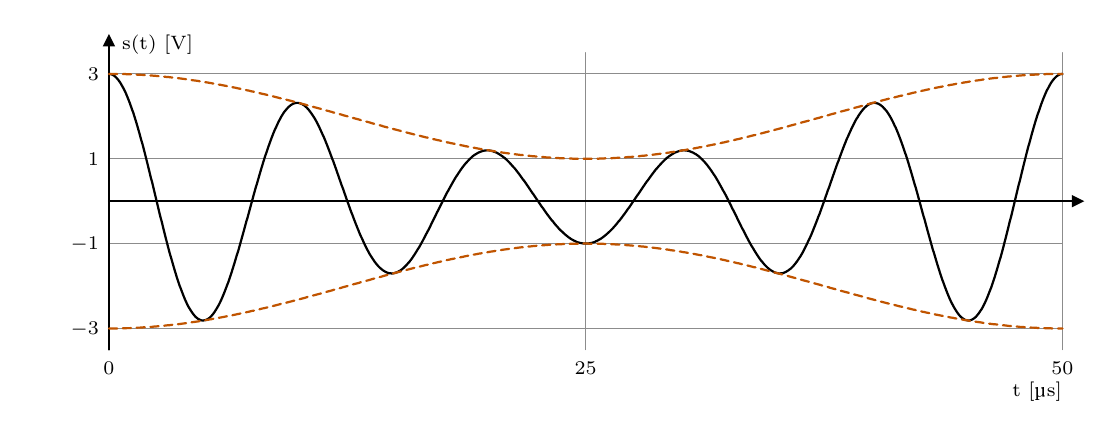
\begin{tikzpicture}[x=0.01985cm,y=-0.01985cm,line cap=round,line join=round]
\useasboundingbox (0,0) rectangle (680,240);
\path[draw=black!45,line width=0.35pt] (52,206) -- (52,16);
\path[draw=black!45,line width=0.35pt] (357,206) -- (357,16);
\path[draw=black!45,line width=0.35pt] (662,206) -- (662,16);
\path[draw=black!45,line width=0.35pt] (52,29.6) -- (662,29.6);
\path[draw=black!45,line width=0.35pt] (52,83.9) -- (662,83.9);
\path[draw=black!45,line width=0.35pt] (52,138.1) -- (662,138.1);
\path[draw=black!45,line width=0.35pt] (52,192.4) -- (662,192.4);
\path[draw=black,line width=0.7pt] (52,111) -- (670,111);
\path[fill=black,draw=none] (676,111) -- (668,107) -- (668,115) -- cycle;
\path[draw=black,line width=0.7pt] (52,206) -- (52,10);
\path[fill=black,draw=none] (52,4) -- (48,12) -- (56,12) -- cycle;
\node[anchor=base,inner sep=0pt,font=\scriptsize] at (52,222) {0};
\node[anchor=base,inner sep=0pt,font=\scriptsize] at (357,222) {25};
\node[anchor=base,inner sep=0pt,font=\scriptsize] at (662,222) {50};
\node[anchor=base east,inner sep=0pt,font=\scriptsize] at (46,33.6) {3};
\node[anchor=base east,inner sep=0pt,font=\scriptsize] at (46,87.9) {1};
\node[anchor=base east,inner sep=0pt,font=\scriptsize] at (46,142.1) {$-$1};
\node[anchor=base east,inner sep=0pt,font=\scriptsize] at (46,196.4) {$-$3};
\node[anchor=base east,inner sep=0pt,font=\scriptsize] at (662,236) {t [\textmu{}s]};
\node[anchor=base west,inner sep=0pt,font=\scriptsize] at (60,14) {s(t) [V]};
\path[draw=black,line width=0.8pt] (52,29.6) -- (52.5,29.6) -- (53,29.7) -- (53.5,29.8) -- (54,30) -- (54.5,30.3) -- (55.1,30.6) -- (55.6,31) -- (56.1,31.4) -- (56.6,31.9) -- (57.1,32.4) -- (57.6,33) -- (58.1,33.6) -- (58.6,34.3) -- (59.1,35) -- (59.6,35.8) -- (60.1,36.7) -- (60.6,37.6) -- (61.2,38.6) -- (61.7,39.6) -- (62.2,40.6) -- (62.7,41.7) -- (63.2,42.9) -- (63.7,44.1) -- (64.2,45.3) -- (64.7,46.6) -- (65.2,47.9) -- (65.7,49.3) -- (66.2,50.7) -- (66.7,52.2) -- (67.3,53.7) -- (67.8,55.2) -- (68.3,56.8) -- (68.8,58.4) -- (69.3,60) -- (69.8,61.7) -- (70.3,63.4) -- (70.8,65.2) -- (71.3,66.9) -- (71.8,68.7) -- (72.3,70.6) -- (72.8,72.4) -- (73.4,74.3) -- (73.9,76.2) -- (74.4,78.2) -- (74.9,80.1) -- (75.4,82.1) -- (75.9,84.1) -- (76.4,86.1) -- (76.9,88.1) -- (77.4,90.2) -- (77.9,92.2) -- (78.4,94.3) -- (78.9,96.4) -- (79.5,98.4) -- (80,100.5) -- (80.5,102.6) -- (81,104.7) -- (81.5,106.8) -- (82,108.9) -- (82.5,111) -- (83,113.1) -- (83.5,115.2) -- (84,117.3) -- (84.5,119.4) -- (85,121.4) -- (85.6,123.5) -- (86.1,125.5) -- (86.6,127.6) -- (87.1,129.6) -- (87.6,131.6) -- (88.1,133.6) -- (88.6,135.6) -- (89.1,137.5) -- (89.6,139.5) -- (90.1,141.4) -- (90.6,143.3) -- (91.1,145.1) -- (91.7,147) -- (92.2,148.8) -- (92.7,150.5) -- (93.2,152.3) -- (93.7,154) -- (94.2,155.7) -- (94.7,157.3) -- (95.2,159) -- (95.7,160.5) -- (96.2,162.1) -- (96.7,163.6) -- (97.2,165.1) -- (97.8,166.5) -- (98.3,167.9) -- (98.8,169.2) -- (99.3,170.5) -- (99.8,171.8) -- (100.3,173) -- (100.8,174.2) -- (101.3,175.3) -- (101.8,176.4) -- (102.3,177.4) -- (102.8,178.4) -- (103.3,179.3) -- (103.9,180.2) -- (104.4,181) -- (104.9,181.8) -- (105.4,182.5) -- (105.9,183.2) -- (106.4,183.8) -- (106.9,184.4) -- (107.4,185) -- (107.9,185.4) -- (108.4,185.8) -- (108.9,186.2) -- (109.4,186.5) -- (110,186.8) -- (110.5,187) -- (111,187.2) -- (111.5,187.3) -- (112,187.3) -- (112.5,187.3) -- (113,187.2) -- (113.5,187.1) -- (114,187) -- (114.5,186.8) -- (115,186.5) -- (115.5,186.2) -- (116.1,185.8) -- (116.6,185.4) -- (117.1,184.9) -- (117.6,184.4) -- (118.1,183.8) -- (118.6,183.2) -- (119.1,182.5) -- (119.6,181.8) -- (120.1,181) -- (120.6,180.2) -- (121.1,179.4) -- (121.6,178.5) -- (122.2,177.5) -- (122.7,176.5) -- (123.2,175.5) -- (123.7,174.4) -- (124.2,173.3) -- (124.7,172.1) -- (125.2,170.9) -- (125.7,169.7) -- (126.2,168.4) -- (126.7,167.1) -- (127.2,165.8) -- (127.7,164.4) -- (128.3,163) -- (128.8,161.5) -- (129.3,160) -- (129.8,158.5) -- (130.3,157) -- (130.8,155.4) -- (131.3,153.8) -- (131.8,152.2) -- (132.3,150.6) -- (132.8,148.9) -- (133.3,147.2) -- (133.8,145.5) -- (134.4,143.8) -- (134.9,142.1) -- (135.4,140.3) -- (135.9,138.5) -- (136.4,136.7) -- (136.9,134.9) -- (137.4,133.1) -- (137.9,131.3) -- (138.4,129.5) -- (138.9,127.6) -- (139.4,125.8) -- (139.9,123.9) -- (140.5,122.1) -- (141,120.2) -- (141.5,118.4) -- (142,116.5) -- (142.5,114.7) -- (143,112.8) -- (143.5,111) -- (144,109.2) -- (144.5,107.3) -- (145,105.5) -- (145.5,103.7) -- (146,101.9) -- (146.6,100.1) -- (147.1,98.3) -- (147.6,96.6) -- (148.1,94.8) -- (148.6,93.1) -- (149.1,91.4) -- (149.6,89.7) -- (150.1,88.1) -- (150.6,86.4) -- (151.1,84.8) -- (151.6,83.2) -- (152.1,81.6) -- (152.7,80.1) -- (153.2,78.6) -- (153.7,77.1) -- (154.2,75.6) -- (154.7,74.2) -- (155.2,72.8) -- (155.7,71.4) -- (156.2,70.1) -- (156.7,68.8) -- (157.2,67.5) -- (157.7,66.3) -- (158.2,65.1) -- (158.8,63.9) -- (159.3,62.8) -- (159.8,61.7) -- (160.3,60.6) -- (160.8,59.6) -- (161.3,58.7) -- (161.8,57.7) -- (162.3,56.8) -- (162.8,56) -- (163.3,55.2) -- (163.8,54.4) -- (164.3,53.7) -- (164.9,53) -- (165.4,52.4) -- (165.9,51.8) -- (166.4,51.3) -- (166.9,50.7) -- (167.4,50.3) -- (167.9,49.9) -- (168.4,49.5) -- (168.9,49.2) -- (169.4,48.9) -- (169.9,48.6) -- (170.4,48.5) -- (171,48.3) -- (171.5,48.2) -- (172,48.1) -- (172.5,48.1) -- (173,48.1) -- (173.5,48.2) -- (174,48.3) -- (174.5,48.5) -- (175,48.7) -- (175.5,48.9) -- (176,49.2) -- (176.5,49.5) -- (177.1,49.9) -- (177.6,50.3) -- (178.1,50.8) -- (178.6,51.2) -- (179.1,51.8) -- (179.6,52.3) -- (180.1,53) -- (180.6,53.6) -- (181.1,54.3) -- (181.6,55) -- (182.1,55.7) -- (182.6,56.5) -- (183.2,57.4) -- (183.7,58.2) -- (184.2,59.1) -- (184.7,60) -- (185.2,61) -- (185.7,62) -- (186.2,63) -- (186.7,64) -- (187.2,65.1) -- (187.7,66.2) -- (188.2,67.3) -- (188.7,68.4) -- (189.3,69.6) -- (189.8,70.8) -- (190.3,72) -- (190.8,73.3) -- (191.3,74.5) -- (191.8,75.8) -- (192.3,77.1) -- (192.8,78.4) -- (193.3,79.7) -- (193.8,81.1) -- (194.3,82.4) -- (194.8,83.8) -- (195.4,85.2) -- (195.9,86.6) -- (196.4,88) -- (196.9,89.4) -- (197.4,90.8) -- (197.9,92.3) -- (198.4,93.7) -- (198.9,95.1) -- (199.4,96.6) -- (199.9,98) -- (200.4,99.5) -- (200.9,100.9) -- (201.5,102.4) -- (202,103.8) -- (202.5,105.3) -- (203,106.7) -- (203.5,108.1) -- (204,109.6) -- (204.5,111) -- (205,112.4) -- (205.5,113.8) -- (206,115.2) -- (206.5,116.6) -- (207,118) -- (207.6,119.4) -- (208.1,120.7) -- (208.6,122.1) -- (209.1,123.4) -- (209.6,124.7) -- (210.1,126) -- (210.6,127.2) -- (211.1,128.5) -- (211.6,129.7) -- (212.1,131) -- (212.6,132.2) -- (213.1,133.3) -- (213.7,134.5) -- (214.2,135.6) -- (214.7,136.7) -- (215.2,137.8) -- (215.7,138.9) -- (216.2,139.9) -- (216.7,140.9) -- (217.2,141.9) -- (217.7,142.8) -- (218.2,143.8) -- (218.7,144.7) -- (219.2,145.5) -- (219.8,146.4) -- (220.3,147.2) -- (220.8,148) -- (221.3,148.7) -- (221.8,149.5) -- (222.3,150.1) -- (222.8,150.8) -- (223.3,151.4) -- (223.8,152) -- (224.3,152.6) -- (224.8,153.1) -- (225.3,153.6) -- (225.9,154.1) -- (226.4,154.5) -- (226.9,154.9) -- (227.4,155.3) -- (227.9,155.6) -- (228.4,155.9) -- (228.9,156.2) -- (229.4,156.4) -- (229.9,156.7) -- (230.4,156.8) -- (230.9,157) -- (231.4,157.1) -- (232,157.1) -- (232.5,157.2) -- (233,157.2) -- (233.5,157.2) -- (234,157.1) -- (234.5,157) -- (235,156.9) -- (235.5,156.7) -- (236,156.6) -- (236.5,156.4) -- (237,156.1) -- (237.5,155.8) -- (238.1,155.5) -- (238.6,155.2) -- (239.1,154.8) -- (239.6,154.5) -- (240.1,154) -- (240.6,153.6) -- (241.1,153.1) -- (241.6,152.6) -- (242.1,152.1) -- (242.6,151.6) -- (243.1,151) -- (243.6,150.4) -- (244.2,149.8) -- (244.7,149.1) -- (245.2,148.5) -- (245.7,147.8) -- (246.2,147.1) -- (246.7,146.3) -- (247.2,145.6) -- (247.7,144.8) -- (248.2,144) -- (248.7,143.2) -- (249.2,142.4) -- (249.7,141.5) -- (250.3,140.7) -- (250.8,139.8) -- (251.3,138.9) -- (251.8,138) -- (252.3,137.1) -- (252.8,136.2) -- (253.3,135.2) -- (253.8,134.3) -- (254.3,133.3) -- (254.8,132.3) -- (255.3,131.4) -- (255.8,130.4) -- (256.4,129.4) -- (256.9,128.4) -- (257.4,127.4) -- (257.9,126.3) -- (258.4,125.3) -- (258.9,124.3) -- (259.4,123.3) -- (259.9,122.3) -- (260.4,121.2) -- (260.9,120.2) -- (261.4,119.2) -- (261.9,118.1) -- (262.5,117.1) -- (263,116.1) -- (263.5,115.1) -- (264,114) -- (264.5,113) -- (265,112) -- (265.5,111) -- (266,110) -- (266.5,109) -- (267,108) -- (267.5,107) -- (268,106.1) -- (268.5,105.1) -- (269.1,104.2) -- (269.6,103.2) -- (270.1,102.3) -- (270.6,101.4) -- (271.1,100.5) -- (271.6,99.6) -- (272.1,98.7) -- (272.6,97.8) -- (273.1,97) -- (273.6,96.1) -- (274.1,95.3) -- (274.7,94.5) -- (275.2,93.7) -- (275.7,92.9) -- (276.2,92.2) -- (276.7,91.4) -- (277.2,90.7) -- (277.7,90) -- (278.2,89.3) -- (278.7,88.7) -- (279.2,88) -- (279.7,87.4) -- (280.2,86.8) -- (280.8,86.2) -- (281.3,85.6) -- (281.8,85.1) -- (282.3,84.5) -- (282.8,84) -- (283.3,83.6) -- (283.8,83.1) -- (284.3,82.6) -- (284.8,82.2) -- (285.3,81.8) -- (285.8,81.5) -- (286.3,81.1) -- (286.9,80.8) -- (287.4,80.5) -- (287.9,80.2) -- (288.4,79.9) -- (288.9,79.7) -- (289.4,79.5) -- (289.9,79.3) -- (290.4,79.1) -- (290.9,78.9) -- (291.4,78.8) -- (291.9,78.7) -- (292.4,78.6) -- (293,78.6) -- (293.5,78.5) -- (294,78.5) -- (294.5,78.5) -- (295,78.5) -- (295.5,78.6) -- (296,78.7) -- (296.5,78.8) -- (297,78.9) -- (297.5,79) -- (298,79.2) -- (298.5,79.4) -- (299.1,79.6) -- (299.6,79.8) -- (300.1,80) -- (300.6,80.3) -- (301.1,80.6) -- (301.6,80.9) -- (302.1,81.2) -- (302.6,81.5) -- (303.1,81.9) -- (303.6,82.2) -- (304.1,82.6) -- (304.6,83) -- (305.2,83.4) -- (305.7,83.9) -- (306.2,84.3) -- (306.7,84.8) -- (307.2,85.3) -- (307.7,85.8) -- (308.2,86.3) -- (308.7,86.9) -- (309.2,87.4) -- (309.7,88) -- (310.2,88.5) -- (310.7,89.1) -- (311.3,89.7) -- (311.8,90.3) -- (312.3,90.9) -- (312.8,91.6) -- (313.3,92.2) -- (313.8,92.9) -- (314.3,93.5) -- (314.8,94.2) -- (315.3,94.9) -- (315.8,95.6) -- (316.3,96.3) -- (316.8,97) -- (317.4,97.7) -- (317.9,98.4) -- (318.4,99.1) -- (318.9,99.8) -- (319.4,100.6) -- (319.9,101.3) -- (320.4,102) -- (320.9,102.8) -- (321.4,103.5) -- (321.9,104.3) -- (322.4,105) -- (322.9,105.8) -- (323.5,106.5) -- (324,107.3) -- (324.5,108) -- (325,108.8) -- (325.5,109.5) -- (326,110.3) -- (326.5,111) -- (327,111.7) -- (327.5,112.5) -- (328,113.2) -- (328.5,114) -- (329,114.7) -- (329.6,115.4) -- (330.1,116.1) -- (330.6,116.9) -- (331.1,117.6) -- (331.6,118.3) -- (332.1,119) -- (332.6,119.7) -- (333.1,120.3) -- (333.6,121) -- (334.1,121.7) -- (334.6,122.3) -- (335.1,123) -- (335.7,123.6) -- (336.2,124.2) -- (336.7,124.9) -- (337.2,125.5) -- (337.7,126.1) -- (338.2,126.7) -- (338.7,127.2) -- (339.2,127.8) -- (339.7,128.4) -- (340.2,128.9) -- (340.7,129.4) -- (341.2,129.9) -- (341.8,130.4) -- (342.3,130.9) -- (342.8,131.4) -- (343.3,131.8) -- (343.8,132.3) -- (344.3,132.7) -- (344.8,133.1) -- (345.3,133.5) -- (345.8,133.9) -- (346.3,134.3) -- (346.8,134.6) -- (347.3,135) -- (347.8,135.3) -- (348.4,135.6) -- (348.9,135.9) -- (349.4,136.2) -- (349.9,136.4) -- (350.4,136.6) -- (350.9,136.9) -- (351.4,137.1) -- (351.9,137.3) -- (352.4,137.4) -- (352.9,137.6) -- (353.4,137.7) -- (354,137.8) -- (354.5,137.9) -- (355,138) -- (355.5,138.1) -- (356,138.1) -- (356.5,138.1) -- (357,138.1) -- (357.5,138.1) -- (358,138.1) -- (358.5,138.1) -- (359,138) -- (359.5,137.9) -- (360.1,137.8) -- (360.6,137.7) -- (361.1,137.6) -- (361.6,137.4) -- (362.1,137.3) -- (362.6,137.1) -- (363.1,136.9) -- (363.6,136.6) -- (364.1,136.4) -- (364.6,136.2) -- (365.1,135.9) -- (365.6,135.6) -- (366.2,135.3) -- (366.7,135) -- (367.2,134.6) -- (367.7,134.3) -- (368.2,133.9) -- (368.7,133.5) -- (369.2,133.1) -- (369.7,132.7) -- (370.2,132.3) -- (370.7,131.8) -- (371.2,131.4) -- (371.7,130.9) -- (372.3,130.4) -- (372.8,129.9) -- (373.3,129.4) -- (373.8,128.9) -- (374.3,128.4) -- (374.8,127.8) -- (375.3,127.2) -- (375.8,126.7) -- (376.3,126.1) -- (376.8,125.5) -- (377.3,124.9) -- (377.8,124.2) -- (378.4,123.6) -- (378.9,123) -- (379.4,122.3) -- (379.9,121.7) -- (380.4,121) -- (380.9,120.3) -- (381.4,119.7) -- (381.9,119) -- (382.4,118.3) -- (382.9,117.6) -- (383.4,116.9) -- (383.9,116.1) -- (384.5,115.4) -- (385,114.7) -- (385.5,114) -- (386,113.2) -- (386.5,112.5) -- (387,111.7) -- (387.5,111) -- (388,110.3) -- (388.5,109.5) -- (389,108.8) -- (389.5,108) -- (390,107.3) -- (390.6,106.5) -- (391.1,105.8) -- (391.6,105) -- (392.1,104.3) -- (392.6,103.5) -- (393.1,102.8) -- (393.6,102) -- (394.1,101.3) -- (394.6,100.6) -- (395.1,99.8) -- (395.6,99.1) -- (396.1,98.4) -- (396.7,97.7) -- (397.2,97) -- (397.7,96.3) -- (398.2,95.6) -- (398.7,94.9) -- (399.2,94.2) -- (399.7,93.5) -- (400.2,92.9) -- (400.7,92.2) -- (401.2,91.6) -- (401.7,90.9) -- (402.2,90.3) -- (402.8,89.7) -- (403.3,89.1) -- (403.8,88.5) -- (404.3,88) -- (404.8,87.4) -- (405.3,86.9) -- (405.8,86.3) -- (406.3,85.8) -- (406.8,85.3) -- (407.3,84.8) -- (407.8,84.3) -- (408.3,83.9) -- (408.8,83.4) -- (409.4,83) -- (409.9,82.6) -- (410.4,82.2) -- (410.9,81.9) -- (411.4,81.5) -- (411.9,81.2) -- (412.4,80.9) -- (412.9,80.6) -- (413.4,80.3) -- (413.9,80) -- (414.4,79.8) -- (415,79.6) -- (415.5,79.4) -- (416,79.2) -- (416.5,79) -- (417,78.9) -- (417.5,78.8) -- (418,78.7) -- (418.5,78.6) -- (419,78.5) -- (419.5,78.5) -- (420,78.5) -- (420.5,78.5) -- (421.1,78.6) -- (421.6,78.6) -- (422.1,78.7) -- (422.6,78.8) -- (423.1,78.9) -- (423.6,79.1) -- (424.1,79.3) -- (424.6,79.5) -- (425.1,79.7) -- (425.6,79.9) -- (426.1,80.2) -- (426.6,80.5) -- (427.2,80.8) -- (427.7,81.1) -- (428.2,81.5) -- (428.7,81.8) -- (429.2,82.2) -- (429.7,82.6) -- (430.2,83.1) -- (430.7,83.6) -- (431.2,84) -- (431.7,84.5) -- (432.2,85.1) -- (432.7,85.6) -- (433.3,86.2) -- (433.8,86.8) -- (434.3,87.4) -- (434.8,88) -- (435.3,88.7) -- (435.8,89.3) -- (436.3,90) -- (436.8,90.7) -- (437.3,91.4) -- (437.8,92.2) -- (438.3,92.9) -- (438.8,93.7) -- (439.4,94.5) -- (439.9,95.3) -- (440.4,96.1) -- (440.9,97) -- (441.4,97.8) -- (441.9,98.7) -- (442.4,99.6) -- (442.9,100.5) -- (443.4,101.4) -- (443.9,102.3) -- (444.4,103.2) -- (444.9,104.2) -- (445.5,105.1) -- (446,106.1) -- (446.5,107) -- (447,108) -- (447.5,109) -- (448,110) -- (448.5,111) -- (449,112) -- (449.5,113) -- (450,114) -- (450.5,115.1) -- (451,116.1) -- (451.6,117.1) -- (452.1,118.1) -- (452.6,119.2) -- (453.1,120.2) -- (453.6,121.2) -- (454.1,122.3) -- (454.6,123.3) -- (455.1,124.3) -- (455.6,125.3) -- (456.1,126.3) -- (456.6,127.4) -- (457.1,128.4) -- (457.7,129.4) -- (458.2,130.4) -- (458.7,131.4) -- (459.2,132.3) -- (459.7,133.3) -- (460.2,134.3) -- (460.7,135.2) -- (461.2,136.2) -- (461.7,137.1) -- (462.2,138) -- (462.7,138.9) -- (463.2,139.8) -- (463.8,140.7) -- (464.3,141.5) -- (464.8,142.4) -- (465.3,143.2) -- (465.8,144) -- (466.3,144.8) -- (466.8,145.6) -- (467.3,146.3) -- (467.8,147.1) -- (468.3,147.8) -- (468.8,148.5) -- (469.3,149.1) -- (469.9,149.8) -- (470.4,150.4) -- (470.9,151) -- (471.4,151.6) -- (471.9,152.1) -- (472.4,152.6) -- (472.9,153.1) -- (473.4,153.6) -- (473.9,154) -- (474.4,154.5) -- (474.9,154.8) -- (475.4,155.2) -- (476,155.5) -- (476.5,155.8) -- (477,156.1) -- (477.5,156.4) -- (478,156.6) -- (478.5,156.7) -- (479,156.9) -- (479.5,157) -- (480,157.1) -- (480.5,157.2) -- (481,157.2) -- (481.5,157.2) -- (482.1,157.1) -- (482.6,157.1) -- (483.1,157) -- (483.6,156.8) -- (484.1,156.7) -- (484.6,156.4) -- (485.1,156.2) -- (485.6,155.9) -- (486.1,155.6) -- (486.6,155.3) -- (487.1,154.9) -- (487.6,154.5) -- (488.2,154.1) -- (488.7,153.6) -- (489.2,153.1) -- (489.7,152.6) -- (490.2,152) -- (490.7,151.4) -- (491.2,150.8) -- (491.7,150.1) -- (492.2,149.5) -- (492.7,148.7) -- (493.2,148) -- (493.7,147.2) -- (494.3,146.4) -- (494.8,145.5) -- (495.3,144.7) -- (495.8,143.8) -- (496.3,142.8) -- (496.8,141.9) -- (497.3,140.9) -- (497.8,139.9) -- (498.3,138.9) -- (498.8,137.8) -- (499.3,136.7) -- (499.8,135.6) -- (500.4,134.5) -- (500.9,133.3) -- (501.4,132.2) -- (501.9,131) -- (502.4,129.7) -- (502.9,128.5) -- (503.4,127.2) -- (503.9,126) -- (504.4,124.7) -- (504.9,123.4) -- (505.4,122.1) -- (505.9,120.7) -- (506.5,119.4) -- (507,118) -- (507.5,116.6) -- (508,115.2) -- (508.5,113.8) -- (509,112.4) -- (509.5,111) -- (510,109.6) -- (510.5,108.1) -- (511,106.7) -- (511.5,105.3) -- (512,103.8) -- (512.6,102.4) -- (513.1,100.9) -- (513.6,99.5) -- (514.1,98) -- (514.6,96.6) -- (515.1,95.1) -- (515.6,93.7) -- (516.1,92.3) -- (516.6,90.8) -- (517.1,89.4) -- (517.6,88) -- (518.1,86.6) -- (518.7,85.2) -- (519.2,83.8) -- (519.7,82.4) -- (520.2,81.1) -- (520.7,79.7) -- (521.2,78.4) -- (521.7,77.1) -- (522.2,75.8) -- (522.7,74.5) -- (523.2,73.3) -- (523.7,72) -- (524.2,70.8) -- (524.8,69.6) -- (525.3,68.4) -- (525.8,67.3) -- (526.3,66.2) -- (526.8,65.1) -- (527.3,64) -- (527.8,63) -- (528.3,62) -- (528.8,61) -- (529.3,60) -- (529.8,59.1) -- (530.3,58.2) -- (530.9,57.4) -- (531.4,56.5) -- (531.9,55.7) -- (532.4,55) -- (532.9,54.3) -- (533.4,53.6) -- (533.9,53) -- (534.4,52.3) -- (534.9,51.8) -- (535.4,51.2) -- (535.9,50.8) -- (536.4,50.3) -- (537,49.9) -- (537.5,49.5) -- (538,49.2) -- (538.5,48.9) -- (539,48.7) -- (539.5,48.5) -- (540,48.3) -- (540.5,48.2) -- (541,48.1) -- (541.5,48.1) -- (542,48.1) -- (542.5,48.2) -- (543.1,48.3) -- (543.6,48.5) -- (544.1,48.6) -- (544.6,48.9) -- (545.1,49.2) -- (545.6,49.5) -- (546.1,49.9) -- (546.6,50.3) -- (547.1,50.7) -- (547.6,51.3) -- (548.1,51.8) -- (548.6,52.4) -- (549.2,53) -- (549.7,53.7) -- (550.2,54.4) -- (550.7,55.2) -- (551.2,56) -- (551.7,56.8) -- (552.2,57.7) -- (552.7,58.7) -- (553.2,59.6) -- (553.7,60.6) -- (554.2,61.7) -- (554.7,62.8) -- (555.3,63.9) -- (555.8,65.1) -- (556.3,66.3) -- (556.8,67.5) -- (557.3,68.8) -- (557.8,70.1) -- (558.3,71.4) -- (558.8,72.8) -- (559.3,74.2) -- (559.8,75.6) -- (560.3,77.1) -- (560.8,78.6) -- (561.3,80.1) -- (561.9,81.6) -- (562.4,83.2) -- (562.9,84.8) -- (563.4,86.4) -- (563.9,88.1) -- (564.4,89.7) -- (564.9,91.4) -- (565.4,93.1) -- (565.9,94.8) -- (566.4,96.6) -- (566.9,98.3) -- (567.4,100.1) -- (568,101.9) -- (568.5,103.7) -- (569,105.5) -- (569.5,107.3) -- (570,109.2) -- (570.5,111) -- (571,112.8) -- (571.5,114.7) -- (572,116.5) -- (572.5,118.4) -- (573,120.2) -- (573.6,122.1) -- (574.1,123.9) -- (574.6,125.8) -- (575.1,127.6) -- (575.6,129.5) -- (576.1,131.3) -- (576.6,133.1) -- (577.1,134.9) -- (577.6,136.7) -- (578.1,138.5) -- (578.6,140.3) -- (579.1,142.1) -- (579.7,143.8) -- (580.2,145.5) -- (580.7,147.2) -- (581.2,148.9) -- (581.7,150.6) -- (582.2,152.2) -- (582.7,153.8) -- (583.2,155.4) -- (583.7,157) -- (584.2,158.5) -- (584.7,160) -- (585.2,161.5) -- (585.8,163) -- (586.3,164.4) -- (586.8,165.8) -- (587.3,167.1) -- (587.8,168.4) -- (588.3,169.7) -- (588.8,170.9) -- (589.3,172.1) -- (589.8,173.3) -- (590.3,174.4) -- (590.8,175.5) -- (591.3,176.5) -- (591.9,177.5) -- (592.4,178.5) -- (592.9,179.4) -- (593.4,180.2) -- (593.9,181) -- (594.4,181.8) -- (594.9,182.5) -- (595.4,183.2) -- (595.9,183.8) -- (596.4,184.4) -- (596.9,184.9) -- (597.4,185.4) -- (598,185.8) -- (598.5,186.2) -- (599,186.5) -- (599.5,186.8) -- (600,187) -- (600.5,187.1) -- (601,187.2) -- (601.5,187.3) -- (602,187.3) -- (602.5,187.3) -- (603,187.2) -- (603.5,187) -- (604.1,186.8) -- (604.6,186.5) -- (605.1,186.2) -- (605.6,185.8) -- (606.1,185.4) -- (606.6,185) -- (607.1,184.4) -- (607.6,183.8) -- (608.1,183.2) -- (608.6,182.5) -- (609.1,181.8) -- (609.6,181) -- (610.2,180.2) -- (610.7,179.3) -- (611.2,178.4) -- (611.7,177.4) -- (612.2,176.4) -- (612.7,175.3) -- (613.2,174.2) -- (613.7,173) -- (614.2,171.8) -- (614.7,170.5) -- (615.2,169.2) -- (615.7,167.9) -- (616.3,166.5) -- (616.8,165.1) -- (617.3,163.6) -- (617.8,162.1) -- (618.3,160.5) -- (618.8,159) -- (619.3,157.3) -- (619.8,155.7) -- (620.3,154) -- (620.8,152.3) -- (621.3,150.5) -- (621.8,148.8) -- (622.4,147) -- (622.9,145.1) -- (623.4,143.3) -- (623.9,141.4) -- (624.4,139.5) -- (624.9,137.5) -- (625.4,135.6) -- (625.9,133.6) -- (626.4,131.6) -- (626.9,129.6) -- (627.4,127.6) -- (627.9,125.5) -- (628.4,123.5) -- (629,121.4) -- (629.5,119.4) -- (630,117.3) -- (630.5,115.2) -- (631,113.1) -- (631.5,111) -- (632,108.9) -- (632.5,106.8) -- (633,104.7) -- (633.5,102.6) -- (634,100.5) -- (634.6,98.4) -- (635.1,96.4) -- (635.6,94.3) -- (636.1,92.2) -- (636.6,90.2) -- (637.1,88.1) -- (637.6,86.1) -- (638.1,84.1) -- (638.6,82.1) -- (639.1,80.1) -- (639.6,78.2) -- (640.1,76.2) -- (640.7,74.3) -- (641.2,72.4) -- (641.7,70.6) -- (642.2,68.7) -- (642.7,66.9) -- (643.2,65.2) -- (643.7,63.4) -- (644.2,61.7) -- (644.7,60) -- (645.2,58.4) -- (645.7,56.8) -- (646.2,55.2) -- (646.8,53.7) -- (647.3,52.2) -- (647.8,50.7) -- (648.3,49.3) -- (648.8,47.9) -- (649.3,46.6) -- (649.8,45.3) -- (650.3,44.1) -- (650.8,42.9) -- (651.3,41.7) -- (651.8,40.6) -- (652.3,39.6) -- (652.9,38.6) -- (653.4,37.6) -- (653.9,36.7) -- (654.4,35.8) -- (654.9,35) -- (655.4,34.3) -- (655.9,33.6) -- (656.4,33) -- (656.9,32.4) -- (657.4,31.9) -- (657.9,31.4) -- (658.4,31) -- (659,30.6) -- (659.5,30.3) -- (660,30) -- (660.5,29.8) -- (661,29.7) -- (661.5,29.6) -- (662,29.6);
\path[draw=cB,line width=0.8pt,dash pattern=on 3pt off 2pt] (52,29.6) -- (52.8,29.6) -- (53.5,29.6) -- (54.3,29.6) -- (55.1,29.6) -- (55.8,29.6) -- (56.6,29.6) -- (57.3,29.6) -- (58.1,29.6) -- (58.9,29.6) -- (59.6,29.7) -- (60.4,29.7) -- (61.2,29.7) -- (61.9,29.7) -- (62.7,29.7) -- (63.4,29.8) -- (64.2,29.8) -- (65,29.8) -- (65.7,29.8) -- (66.5,29.9) -- (67.3,29.9) -- (68,29.9) -- (68.8,30) -- (69.5,30) -- (70.3,30.1) -- (71.1,30.1) -- (71.8,30.1) -- (72.6,30.2) -- (73.4,30.2) -- (74.1,30.3) -- (74.9,30.3) -- (75.6,30.4) -- (76.4,30.4) -- (77.2,30.5) -- (77.9,30.5) -- (78.7,30.6) -- (79.5,30.6) -- (80.2,30.7) -- (81,30.8) -- (81.7,30.8) -- (82.5,30.9) -- (83.3,31) -- (84,31) -- (84.8,31.1) -- (85.6,31.2) -- (86.3,31.2) -- (87.1,31.3) -- (87.8,31.4) -- (88.6,31.5) -- (89.4,31.6) -- (90.1,31.6) -- (90.9,31.7) -- (91.7,31.8) -- (92.4,31.9) -- (93.2,32) -- (93.9,32.1) -- (94.7,32.2) -- (95.5,32.2) -- (96.2,32.3) -- (97,32.4) -- (97.8,32.5) -- (98.5,32.6) -- (99.3,32.7) -- (100,32.8) -- (100.8,32.9) -- (101.6,33) -- (102.3,33.1) -- (103.1,33.2) -- (103.9,33.4) -- (104.6,33.5) -- (105.4,33.6) -- (106.1,33.7) -- (106.9,33.8) -- (107.7,33.9) -- (108.4,34) -- (109.2,34.1) -- (110,34.3) -- (110.7,34.4) -- (111.5,34.5) -- (112.2,34.6) -- (113,34.8) -- (113.8,34.9) -- (114.5,35) -- (115.3,35.1) -- (116.1,35.3) -- (116.8,35.4) -- (117.6,35.5) -- (118.3,35.7) -- (119.1,35.8) -- (119.9,35.9) -- (120.6,36.1) -- (121.4,36.2) -- (122.2,36.4) -- (122.9,36.5) -- (123.7,36.6) -- (124.4,36.8) -- (125.2,36.9) -- (126,37.1) -- (126.7,37.2) -- (127.5,37.4) -- (128.3,37.5) -- (129,37.7) -- (129.8,37.8) -- (130.5,38) -- (131.3,38.1) -- (132.1,38.3) -- (132.8,38.4) -- (133.6,38.6) -- (134.4,38.8) -- (135.1,38.9) -- (135.9,39.1) -- (136.6,39.2) -- (137.4,39.4) -- (138.2,39.6) -- (138.9,39.7) -- (139.7,39.9) -- (140.5,40.1) -- (141.2,40.2) -- (142,40.4) -- (142.7,40.6) -- (143.5,40.8) -- (144.3,40.9) -- (145,41.1) -- (145.8,41.3) -- (146.6,41.5) -- (147.3,41.6) -- (148.1,41.8) -- (148.8,42) -- (149.6,42.2) -- (150.4,42.4) -- (151.1,42.5) -- (151.9,42.7) -- (152.7,42.9) -- (153.4,43.1) -- (154.2,43.3) -- (154.9,43.5) -- (155.7,43.6) -- (156.5,43.8) -- (157.2,44) -- (158,44.2) -- (158.8,44.4) -- (159.5,44.6) -- (160.3,44.8) -- (161,45) -- (161.8,45.2) -- (162.6,45.4) -- (163.3,45.5) -- (164.1,45.7) -- (164.9,45.9) -- (165.6,46.1) -- (166.4,46.3) -- (167.1,46.5) -- (167.9,46.7) -- (168.7,46.9) -- (169.4,47.1) -- (170.2,47.3) -- (171,47.5) -- (171.7,47.7) -- (172.5,47.9) -- (173.2,48.1) -- (174,48.3) -- (174.8,48.5) -- (175.5,48.7) -- (176.3,48.9) -- (177.1,49.1) -- (177.8,49.3) -- (178.6,49.6) -- (179.3,49.8) -- (180.1,50) -- (180.9,50.2) -- (181.6,50.4) -- (182.4,50.6) -- (183.2,50.8) -- (183.9,51) -- (184.7,51.2) -- (185.4,51.4) -- (186.2,51.6) -- (187,51.8) -- (187.7,52) -- (188.5,52.3) -- (189.3,52.5) -- (190,52.7) -- (190.8,52.9) -- (191.5,53.1) -- (192.3,53.3) -- (193.1,53.5) -- (193.8,53.7) -- (194.6,53.9) -- (195.4,54.2) -- (196.1,54.4) -- (196.9,54.6) -- (197.6,54.8) -- (198.4,55) -- (199.2,55.2) -- (199.9,55.4) -- (200.7,55.6) -- (201.5,55.9) -- (202.2,56.1) -- (203,56.3) -- (203.7,56.5) -- (204.5,56.7) -- (205.3,56.9) -- (206,57.1) -- (206.8,57.4) -- (207.6,57.6) -- (208.3,57.8) -- (209.1,58) -- (209.8,58.2) -- (210.6,58.4) -- (211.4,58.6) -- (212.1,58.8) -- (212.9,59.1) -- (213.7,59.3) -- (214.4,59.5) -- (215.2,59.7) -- (215.9,59.9) -- (216.7,60.1) -- (217.5,60.3) -- (218.2,60.5) -- (219,60.7) -- (219.8,61) -- (220.5,61.2) -- (221.3,61.4) -- (222,61.6) -- (222.8,61.8) -- (223.6,62) -- (224.3,62.2) -- (225.1,62.4) -- (225.9,62.6) -- (226.6,62.8) -- (227.4,63.1) -- (228.1,63.3) -- (228.9,63.5) -- (229.7,63.7) -- (230.4,63.9) -- (231.2,64.1) -- (232,64.3) -- (232.7,64.5) -- (233.5,64.7) -- (234.2,64.9) -- (235,65.1) -- (235.8,65.3) -- (236.5,65.5) -- (237.3,65.7) -- (238.1,65.9) -- (238.8,66.1) -- (239.6,66.3) -- (240.3,66.5) -- (241.1,66.7) -- (241.9,66.9) -- (242.6,67.1) -- (243.4,67.3) -- (244.2,67.5) -- (244.9,67.7) -- (245.7,67.9) -- (246.4,68.1) -- (247.2,68.3) -- (248,68.5) -- (248.7,68.7) -- (249.5,68.8) -- (250.3,69) -- (251,69.2) -- (251.8,69.4) -- (252.5,69.6) -- (253.3,69.8) -- (254.1,70) -- (254.8,70.2) -- (255.6,70.3) -- (256.4,70.5) -- (257.1,70.7) -- (257.9,70.9) -- (258.6,71.1) -- (259.4,71.3) -- (260.2,71.4) -- (260.9,71.6) -- (261.7,71.8) -- (262.5,72) -- (263.2,72.1) -- (264,72.3) -- (264.7,72.5) -- (265.5,72.7) -- (266.3,72.8) -- (267,73) -- (267.8,73.2) -- (268.5,73.4) -- (269.3,73.5) -- (270.1,73.7) -- (270.8,73.9) -- (271.6,74) -- (272.4,74.2) -- (273.1,74.3) -- (273.9,74.5) -- (274.7,74.7) -- (275.4,74.8) -- (276.2,75) -- (276.9,75.1) -- (277.7,75.3) -- (278.5,75.4) -- (279.2,75.6) -- (280,75.8) -- (280.8,75.9) -- (281.5,76.1) -- (282.3,76.2) -- (283,76.4) -- (283.8,76.5) -- (284.6,76.6) -- (285.3,76.8) -- (286.1,76.9) -- (286.9,77.1) -- (287.6,77.2) -- (288.4,77.4) -- (289.1,77.5) -- (289.9,77.6) -- (290.7,77.8) -- (291.4,77.9) -- (292.2,78) -- (293,78.2) -- (293.7,78.3) -- (294.5,78.4) -- (295.2,78.5) -- (296,78.7) -- (296.8,78.8) -- (297.5,78.9) -- (298.3,79) -- (299.1,79.2) -- (299.8,79.3) -- (300.6,79.4) -- (301.3,79.5) -- (302.1,79.6) -- (302.9,79.7) -- (303.6,79.9) -- (304.4,80) -- (305.2,80.1) -- (305.9,80.2) -- (306.7,80.3) -- (307.4,80.4) -- (308.2,80.5) -- (309,80.6) -- (309.7,80.7) -- (310.5,80.8) -- (311.3,80.9) -- (312,81) -- (312.8,81.1) -- (313.5,81.2) -- (314.3,81.3) -- (315.1,81.4) -- (315.8,81.5) -- (316.6,81.5) -- (317.4,81.6) -- (318.1,81.7) -- (318.9,81.8) -- (319.6,81.9) -- (320.4,82) -- (321.2,82) -- (321.9,82.1) -- (322.7,82.2) -- (323.5,82.3) -- (324.2,82.3) -- (325,82.4) -- (325.7,82.5) -- (326.5,82.5) -- (327.3,82.6) -- (328,82.7) -- (328.8,82.7) -- (329.6,82.8) -- (330.3,82.8) -- (331.1,82.9) -- (331.8,83) -- (332.6,83) -- (333.4,83.1) -- (334.1,83.1) -- (334.9,83.2) -- (335.7,83.2) -- (336.4,83.2) -- (337.2,83.3) -- (337.9,83.3) -- (338.7,83.4) -- (339.5,83.4) -- (340.2,83.5) -- (341,83.5) -- (341.8,83.5) -- (342.5,83.6) -- (343.3,83.6) -- (344,83.6) -- (344.8,83.6) -- (345.6,83.7) -- (346.3,83.7) -- (347.1,83.7) -- (347.8,83.7) -- (348.6,83.8) -- (349.4,83.8) -- (350.1,83.8) -- (350.9,83.8) -- (351.7,83.8) -- (352.4,83.8) -- (353.2,83.8) -- (354,83.8) -- (354.7,83.8) -- (355.5,83.9) -- (356.2,83.9) -- (357,83.9) -- (357.8,83.9) -- (358.5,83.9) -- (359.3,83.8) -- (360.1,83.8) -- (360.8,83.8) -- (361.6,83.8) -- (362.3,83.8) -- (363.1,83.8) -- (363.9,83.8) -- (364.6,83.8) -- (365.4,83.8) -- (366.2,83.7) -- (366.9,83.7) -- (367.7,83.7) -- (368.4,83.7) -- (369.2,83.6) -- (370,83.6) -- (370.7,83.6) -- (371.5,83.6) -- (372.3,83.5) -- (373,83.5) -- (373.8,83.5) -- (374.5,83.4) -- (375.3,83.4) -- (376.1,83.3) -- (376.8,83.3) -- (377.6,83.2) -- (378.4,83.2) -- (379.1,83.2) -- (379.9,83.1) -- (380.6,83.1) -- (381.4,83) -- (382.2,83) -- (382.9,82.9) -- (383.7,82.8) -- (384.5,82.8) -- (385.2,82.7) -- (386,82.7) -- (386.7,82.6) -- (387.5,82.5) -- (388.3,82.5) -- (389,82.4) -- (389.8,82.3) -- (390.6,82.3) -- (391.3,82.2) -- (392.1,82.1) -- (392.8,82) -- (393.6,82) -- (394.4,81.9) -- (395.1,81.8) -- (395.9,81.7) -- (396.7,81.6) -- (397.4,81.5) -- (398.2,81.5) -- (398.9,81.4) -- (399.7,81.3) -- (400.5,81.2) -- (401.2,81.1) -- (402,81) -- (402.8,80.9) -- (403.5,80.8) -- (404.3,80.7) -- (405,80.6) -- (405.8,80.5) -- (406.6,80.4) -- (407.3,80.3) -- (408.1,80.2) -- (408.8,80.1) -- (409.6,80) -- (410.4,79.9) -- (411.1,79.7) -- (411.9,79.6) -- (412.7,79.5) -- (413.4,79.4) -- (414.2,79.3) -- (415,79.2) -- (415.7,79) -- (416.5,78.9) -- (417.2,78.8) -- (418,78.7) -- (418.8,78.5) -- (419.5,78.4) -- (420.3,78.3) -- (421.1,78.2) -- (421.8,78) -- (422.6,77.9) -- (423.3,77.8) -- (424.1,77.6) -- (424.9,77.5) -- (425.6,77.4) -- (426.4,77.2) -- (427.2,77.1) -- (427.9,76.9) -- (428.7,76.8) -- (429.4,76.6) -- (430.2,76.5) -- (431,76.4) -- (431.7,76.2) -- (432.5,76.1) -- (433.3,75.9) -- (434,75.8) -- (434.8,75.6) -- (435.5,75.4) -- (436.3,75.3) -- (437.1,75.1) -- (437.8,75) -- (438.6,74.8) -- (439.4,74.7) -- (440.1,74.5) -- (440.9,74.3) -- (441.6,74.2) -- (442.4,74) -- (443.2,73.9) -- (443.9,73.7) -- (444.7,73.5) -- (445.5,73.4) -- (446.2,73.2) -- (447,73) -- (447.7,72.8) -- (448.5,72.7) -- (449.3,72.5) -- (450,72.3) -- (450.8,72.1) -- (451.6,72) -- (452.3,71.8) -- (453.1,71.6) -- (453.8,71.4) -- (454.6,71.3) -- (455.4,71.1) -- (456.1,70.9) -- (456.9,70.7) -- (457.7,70.5) -- (458.4,70.3) -- (459.2,70.2) -- (459.9,70) -- (460.7,69.8) -- (461.5,69.6) -- (462.2,69.4) -- (463,69.2) -- (463.8,69) -- (464.5,68.8) -- (465.3,68.7) -- (466,68.5) -- (466.8,68.3) -- (467.6,68.1) -- (468.3,67.9) -- (469.1,67.7) -- (469.9,67.5) -- (470.6,67.3) -- (471.4,67.1) -- (472.1,66.9) -- (472.9,66.7) -- (473.7,66.5) -- (474.4,66.3) -- (475.2,66.1) -- (476,65.9) -- (476.7,65.7) -- (477.5,65.5) -- (478.2,65.3) -- (479,65.1) -- (479.8,64.9) -- (480.5,64.7) -- (481.3,64.5) -- (482.1,64.3) -- (482.8,64.1) -- (483.6,63.9) -- (484.3,63.7) -- (485.1,63.5) -- (485.9,63.3) -- (486.6,63.1) -- (487.4,62.8) -- (488.2,62.6) -- (488.9,62.4) -- (489.7,62.2) -- (490.4,62) -- (491.2,61.8) -- (492,61.6) -- (492.7,61.4) -- (493.5,61.2) -- (494.3,61) -- (495,60.7) -- (495.8,60.5) -- (496.5,60.3) -- (497.3,60.1) -- (498.1,59.9) -- (498.8,59.7) -- (499.6,59.5) -- (500.4,59.3) -- (501.1,59.1) -- (501.9,58.8) -- (502.6,58.6) -- (503.4,58.4) -- (504.2,58.2) -- (504.9,58) -- (505.7,57.8) -- (506.5,57.6) -- (507.2,57.4) -- (508,57.1) -- (508.7,56.9) -- (509.5,56.7) -- (510.3,56.5) -- (511,56.3) -- (511.8,56.1) -- (512.6,55.9) -- (513.3,55.6) -- (514.1,55.4) -- (514.8,55.2) -- (515.6,55) -- (516.4,54.8) -- (517.1,54.6) -- (517.9,54.4) -- (518.7,54.2) -- (519.4,53.9) -- (520.2,53.7) -- (520.9,53.5) -- (521.7,53.3) -- (522.5,53.1) -- (523.2,52.9) -- (524,52.7) -- (524.8,52.5) -- (525.5,52.3) -- (526.3,52) -- (527,51.8) -- (527.8,51.6) -- (528.6,51.4) -- (529.3,51.2) -- (530.1,51) -- (530.9,50.8) -- (531.6,50.6) -- (532.4,50.4) -- (533.1,50.2) -- (533.9,50) -- (534.7,49.8) -- (535.4,49.6) -- (536.2,49.3) -- (537,49.1) -- (537.7,48.9) -- (538.5,48.7) -- (539.2,48.5) -- (540,48.3) -- (540.8,48.1) -- (541.5,47.9) -- (542.3,47.7) -- (543.1,47.5) -- (543.8,47.3) -- (544.6,47.1) -- (545.3,46.9) -- (546.1,46.7) -- (546.9,46.5) -- (547.6,46.3) -- (548.4,46.1) -- (549.2,45.9) -- (549.9,45.7) -- (550.7,45.5) -- (551.4,45.4) -- (552.2,45.2) -- (553,45) -- (553.7,44.8) -- (554.5,44.6) -- (555.3,44.4) -- (556,44.2) -- (556.8,44) -- (557.5,43.8) -- (558.3,43.6) -- (559.1,43.5) -- (559.8,43.3) -- (560.6,43.1) -- (561.3,42.9) -- (562.1,42.7) -- (562.9,42.5) -- (563.6,42.4) -- (564.4,42.2) -- (565.2,42) -- (565.9,41.8) -- (566.7,41.6) -- (567.4,41.5) -- (568.2,41.3) -- (569,41.1) -- (569.7,40.9) -- (570.5,40.8) -- (571.3,40.6) -- (572,40.4) -- (572.8,40.2) -- (573.6,40.1) -- (574.3,39.9) -- (575.1,39.7) -- (575.8,39.6) -- (576.6,39.4) -- (577.4,39.2) -- (578.1,39.1) -- (578.9,38.9) -- (579.7,38.8) -- (580.4,38.6) -- (581.2,38.4) -- (581.9,38.3) -- (582.7,38.1) -- (583.5,38) -- (584.2,37.8) -- (585,37.7) -- (585.8,37.5) -- (586.5,37.4) -- (587.3,37.2) -- (588,37.1) -- (588.8,36.9) -- (589.6,36.8) -- (590.3,36.6) -- (591.1,36.5) -- (591.9,36.4) -- (592.6,36.2) -- (593.4,36.1) -- (594.1,35.9) -- (594.9,35.8) -- (595.7,35.7) -- (596.4,35.5) -- (597.2,35.4) -- (598,35.3) -- (598.7,35.1) -- (599.5,35) -- (600.2,34.9) -- (601,34.8) -- (601.8,34.6) -- (602.5,34.5) -- (603.3,34.4) -- (604.1,34.3) -- (604.8,34.1) -- (605.6,34) -- (606.3,33.9) -- (607.1,33.8) -- (607.9,33.7) -- (608.6,33.6) -- (609.4,33.5) -- (610.2,33.4) -- (610.9,33.2) -- (611.7,33.1) -- (612.4,33) -- (613.2,32.9) -- (614,32.8) -- (614.7,32.7) -- (615.5,32.6) -- (616.3,32.5) -- (617,32.4) -- (617.8,32.3) -- (618.5,32.2) -- (619.3,32.2) -- (620.1,32.1) -- (620.8,32) -- (621.6,31.9) -- (622.4,31.8) -- (623.1,31.7) -- (623.9,31.6) -- (624.6,31.6) -- (625.4,31.5) -- (626.2,31.4) -- (626.9,31.3) -- (627.7,31.2) -- (628.4,31.2) -- (629.2,31.1) -- (630,31) -- (630.7,31) -- (631.5,30.9) -- (632.3,30.8) -- (633,30.8) -- (633.8,30.7) -- (634.6,30.6) -- (635.3,30.6) -- (636.1,30.5) -- (636.8,30.5) -- (637.6,30.4) -- (638.4,30.4) -- (639.1,30.3) -- (639.9,30.3) -- (640.7,30.2) -- (641.4,30.2) -- (642.2,30.1) -- (642.9,30.1) -- (643.7,30.1) -- (644.5,30) -- (645.2,30) -- (646,29.9) -- (646.8,29.9) -- (647.5,29.9) -- (648.3,29.8) -- (649,29.8) -- (649.8,29.8) -- (650.6,29.8) -- (651.3,29.7) -- (652.1,29.7) -- (652.9,29.7) -- (653.6,29.7) -- (654.4,29.7) -- (655.1,29.6) -- (655.9,29.6) -- (656.7,29.6) -- (657.4,29.6) -- (658.2,29.6) -- (659,29.6) -- (659.7,29.6) -- (660.5,29.6) -- (661.2,29.6) -- (662,29.6);
\path[draw=cB,line width=0.8pt,dash pattern=on 3pt off 2pt] (52,192.4) -- (52.8,192.4) -- (53.5,192.4) -- (54.3,192.4) -- (55.1,192.4) -- (55.8,192.4) -- (56.6,192.4) -- (57.3,192.4) -- (58.1,192.4) -- (58.9,192.4) -- (59.6,192.3) -- (60.4,192.3) -- (61.2,192.3) -- (61.9,192.3) -- (62.7,192.3) -- (63.4,192.2) -- (64.2,192.2) -- (65,192.2) -- (65.7,192.2) -- (66.5,192.1) -- (67.3,192.1) -- (68,192.1) -- (68.8,192) -- (69.5,192) -- (70.3,191.9) -- (71.1,191.9) -- (71.8,191.9) -- (72.6,191.8) -- (73.4,191.8) -- (74.1,191.7) -- (74.9,191.7) -- (75.6,191.6) -- (76.4,191.6) -- (77.2,191.5) -- (77.9,191.5) -- (78.7,191.4) -- (79.5,191.4) -- (80.2,191.3) -- (81,191.2) -- (81.7,191.2) -- (82.5,191.1) -- (83.3,191) -- (84,191) -- (84.8,190.9) -- (85.6,190.8) -- (86.3,190.8) -- (87.1,190.7) -- (87.8,190.6) -- (88.6,190.5) -- (89.4,190.4) -- (90.1,190.4) -- (90.9,190.3) -- (91.7,190.2) -- (92.4,190.1) -- (93.2,190) -- (93.9,189.9) -- (94.7,189.8) -- (95.5,189.8) -- (96.2,189.7) -- (97,189.6) -- (97.8,189.5) -- (98.5,189.4) -- (99.3,189.3) -- (100,189.2) -- (100.8,189.1) -- (101.6,189) -- (102.3,188.9) -- (103.1,188.8) -- (103.9,188.6) -- (104.6,188.5) -- (105.4,188.4) -- (106.1,188.3) -- (106.9,188.2) -- (107.7,188.1) -- (108.4,188) -- (109.2,187.9) -- (110,187.7) -- (110.7,187.6) -- (111.5,187.5) -- (112.2,187.4) -- (113,187.2) -- (113.8,187.1) -- (114.5,187) -- (115.3,186.9) -- (116.1,186.7) -- (116.8,186.6) -- (117.6,186.5) -- (118.3,186.3) -- (119.1,186.2) -- (119.9,186.1) -- (120.6,185.9) -- (121.4,185.8) -- (122.2,185.6) -- (122.9,185.5) -- (123.7,185.4) -- (124.4,185.2) -- (125.2,185.1) -- (126,184.9) -- (126.7,184.8) -- (127.5,184.6) -- (128.3,184.5) -- (129,184.3) -- (129.8,184.2) -- (130.5,184) -- (131.3,183.9) -- (132.1,183.7) -- (132.8,183.6) -- (133.6,183.4) -- (134.4,183.2) -- (135.1,183.1) -- (135.9,182.9) -- (136.6,182.8) -- (137.4,182.6) -- (138.2,182.4) -- (138.9,182.3) -- (139.7,182.1) -- (140.5,181.9) -- (141.2,181.8) -- (142,181.6) -- (142.7,181.4) -- (143.5,181.2) -- (144.3,181.1) -- (145,180.9) -- (145.8,180.7) -- (146.6,180.5) -- (147.3,180.4) -- (148.1,180.2) -- (148.8,180) -- (149.6,179.8) -- (150.4,179.6) -- (151.1,179.5) -- (151.9,179.3) -- (152.7,179.1) -- (153.4,178.9) -- (154.2,178.7) -- (154.9,178.5) -- (155.7,178.4) -- (156.5,178.2) -- (157.2,178) -- (158,177.8) -- (158.8,177.6) -- (159.5,177.4) -- (160.3,177.2) -- (161,177) -- (161.8,176.8) -- (162.6,176.6) -- (163.3,176.5) -- (164.1,176.3) -- (164.9,176.1) -- (165.6,175.9) -- (166.4,175.7) -- (167.1,175.5) -- (167.9,175.3) -- (168.7,175.1) -- (169.4,174.9) -- (170.2,174.7) -- (171,174.5) -- (171.7,174.3) -- (172.5,174.1) -- (173.2,173.9) -- (174,173.7) -- (174.8,173.5) -- (175.5,173.3) -- (176.3,173.1) -- (177.1,172.9) -- (177.8,172.7) -- (178.6,172.4) -- (179.3,172.2) -- (180.1,172) -- (180.9,171.8) -- (181.6,171.6) -- (182.4,171.4) -- (183.2,171.2) -- (183.9,171) -- (184.7,170.8) -- (185.4,170.6) -- (186.2,170.4) -- (187,170.2) -- (187.7,170) -- (188.5,169.7) -- (189.3,169.5) -- (190,169.3) -- (190.8,169.1) -- (191.5,168.9) -- (192.3,168.7) -- (193.1,168.5) -- (193.8,168.3) -- (194.6,168.1) -- (195.4,167.8) -- (196.1,167.6) -- (196.9,167.4) -- (197.6,167.2) -- (198.4,167) -- (199.2,166.8) -- (199.9,166.6) -- (200.7,166.4) -- (201.5,166.1) -- (202.2,165.9) -- (203,165.7) -- (203.7,165.5) -- (204.5,165.3) -- (205.3,165.1) -- (206,164.9) -- (206.8,164.6) -- (207.6,164.4) -- (208.3,164.2) -- (209.1,164) -- (209.8,163.8) -- (210.6,163.6) -- (211.4,163.4) -- (212.1,163.2) -- (212.9,162.9) -- (213.7,162.7) -- (214.4,162.5) -- (215.2,162.3) -- (215.9,162.1) -- (216.7,161.9) -- (217.5,161.7) -- (218.2,161.5) -- (219,161.3) -- (219.8,161) -- (220.5,160.8) -- (221.3,160.6) -- (222,160.4) -- (222.8,160.2) -- (223.6,160) -- (224.3,159.8) -- (225.1,159.6) -- (225.9,159.4) -- (226.6,159.2) -- (227.4,158.9) -- (228.1,158.7) -- (228.9,158.5) -- (229.7,158.3) -- (230.4,158.1) -- (231.2,157.9) -- (232,157.7) -- (232.7,157.5) -- (233.5,157.3) -- (234.2,157.1) -- (235,156.9) -- (235.8,156.7) -- (236.5,156.5) -- (237.3,156.3) -- (238.1,156.1) -- (238.8,155.9) -- (239.6,155.7) -- (240.3,155.5) -- (241.1,155.3) -- (241.9,155.1) -- (242.6,154.9) -- (243.4,154.7) -- (244.2,154.5) -- (244.9,154.3) -- (245.7,154.1) -- (246.4,153.9) -- (247.2,153.7) -- (248,153.5) -- (248.7,153.3) -- (249.5,153.2) -- (250.3,153) -- (251,152.8) -- (251.8,152.6) -- (252.5,152.4) -- (253.3,152.2) -- (254.1,152) -- (254.8,151.8) -- (255.6,151.7) -- (256.4,151.5) -- (257.1,151.3) -- (257.9,151.1) -- (258.6,150.9) -- (259.4,150.7) -- (260.2,150.6) -- (260.9,150.4) -- (261.7,150.2) -- (262.5,150) -- (263.2,149.9) -- (264,149.7) -- (264.7,149.5) -- (265.5,149.3) -- (266.3,149.2) -- (267,149) -- (267.8,148.8) -- (268.5,148.6) -- (269.3,148.5) -- (270.1,148.3) -- (270.8,148.1) -- (271.6,148) -- (272.4,147.8) -- (273.1,147.7) -- (273.9,147.5) -- (274.7,147.3) -- (275.4,147.2) -- (276.2,147) -- (276.9,146.9) -- (277.7,146.7) -- (278.5,146.6) -- (279.2,146.4) -- (280,146.2) -- (280.8,146.1) -- (281.5,145.9) -- (282.3,145.8) -- (283,145.6) -- (283.8,145.5) -- (284.6,145.4) -- (285.3,145.2) -- (286.1,145.1) -- (286.9,144.9) -- (287.6,144.8) -- (288.4,144.6) -- (289.1,144.5) -- (289.9,144.4) -- (290.7,144.2) -- (291.4,144.1) -- (292.2,144) -- (293,143.8) -- (293.7,143.7) -- (294.5,143.6) -- (295.2,143.5) -- (296,143.3) -- (296.8,143.2) -- (297.5,143.1) -- (298.3,143) -- (299.1,142.8) -- (299.8,142.7) -- (300.6,142.6) -- (301.3,142.5) -- (302.1,142.4) -- (302.9,142.3) -- (303.6,142.1) -- (304.4,142) -- (305.2,141.9) -- (305.9,141.8) -- (306.7,141.7) -- (307.4,141.6) -- (308.2,141.5) -- (309,141.4) -- (309.7,141.3) -- (310.5,141.2) -- (311.3,141.1) -- (312,141) -- (312.8,140.9) -- (313.5,140.8) -- (314.3,140.7) -- (315.1,140.6) -- (315.8,140.5) -- (316.6,140.5) -- (317.4,140.4) -- (318.1,140.3) -- (318.9,140.2) -- (319.6,140.1) -- (320.4,140) -- (321.2,140) -- (321.9,139.9) -- (322.7,139.8) -- (323.5,139.7) -- (324.2,139.7) -- (325,139.6) -- (325.7,139.5) -- (326.5,139.5) -- (327.3,139.4) -- (328,139.3) -- (328.8,139.3) -- (329.6,139.2) -- (330.3,139.2) -- (331.1,139.1) -- (331.8,139) -- (332.6,139) -- (333.4,138.9) -- (334.1,138.9) -- (334.9,138.8) -- (335.7,138.8) -- (336.4,138.8) -- (337.2,138.7) -- (337.9,138.7) -- (338.7,138.6) -- (339.5,138.6) -- (340.2,138.5) -- (341,138.5) -- (341.8,138.5) -- (342.5,138.4) -- (343.3,138.4) -- (344,138.4) -- (344.8,138.4) -- (345.6,138.3) -- (346.3,138.3) -- (347.1,138.3) -- (347.8,138.3) -- (348.6,138.2) -- (349.4,138.2) -- (350.1,138.2) -- (350.9,138.2) -- (351.7,138.2) -- (352.4,138.2) -- (353.2,138.2) -- (354,138.2) -- (354.7,138.2) -- (355.5,138.1) -- (356.2,138.1) -- (357,138.1) -- (357.8,138.1) -- (358.5,138.1) -- (359.3,138.2) -- (360.1,138.2) -- (360.8,138.2) -- (361.6,138.2) -- (362.3,138.2) -- (363.1,138.2) -- (363.9,138.2) -- (364.6,138.2) -- (365.4,138.2) -- (366.2,138.3) -- (366.9,138.3) -- (367.7,138.3) -- (368.4,138.3) -- (369.2,138.4) -- (370,138.4) -- (370.7,138.4) -- (371.5,138.4) -- (372.3,138.5) -- (373,138.5) -- (373.8,138.5) -- (374.5,138.6) -- (375.3,138.6) -- (376.1,138.7) -- (376.8,138.7) -- (377.6,138.8) -- (378.4,138.8) -- (379.1,138.8) -- (379.9,138.9) -- (380.6,138.9) -- (381.4,139) -- (382.2,139) -- (382.9,139.1) -- (383.7,139.2) -- (384.5,139.2) -- (385.2,139.3) -- (386,139.3) -- (386.7,139.4) -- (387.5,139.5) -- (388.3,139.5) -- (389,139.6) -- (389.8,139.7) -- (390.6,139.7) -- (391.3,139.8) -- (392.1,139.9) -- (392.8,140) -- (393.6,140) -- (394.4,140.1) -- (395.1,140.2) -- (395.9,140.3) -- (396.7,140.4) -- (397.4,140.5) -- (398.2,140.5) -- (398.9,140.6) -- (399.7,140.7) -- (400.5,140.8) -- (401.2,140.9) -- (402,141) -- (402.8,141.1) -- (403.5,141.2) -- (404.3,141.3) -- (405,141.4) -- (405.8,141.5) -- (406.6,141.6) -- (407.3,141.7) -- (408.1,141.8) -- (408.8,141.9) -- (409.6,142) -- (410.4,142.1) -- (411.1,142.3) -- (411.9,142.4) -- (412.7,142.5) -- (413.4,142.6) -- (414.2,142.7) -- (415,142.8) -- (415.7,143) -- (416.5,143.1) -- (417.2,143.2) -- (418,143.3) -- (418.8,143.5) -- (419.5,143.6) -- (420.3,143.7) -- (421.1,143.8) -- (421.8,144) -- (422.6,144.1) -- (423.3,144.2) -- (424.1,144.4) -- (424.9,144.5) -- (425.6,144.6) -- (426.4,144.8) -- (427.2,144.9) -- (427.9,145.1) -- (428.7,145.2) -- (429.4,145.4) -- (430.2,145.5) -- (431,145.6) -- (431.7,145.8) -- (432.5,145.9) -- (433.3,146.1) -- (434,146.2) -- (434.8,146.4) -- (435.5,146.6) -- (436.3,146.7) -- (437.1,146.9) -- (437.8,147) -- (438.6,147.2) -- (439.4,147.3) -- (440.1,147.5) -- (440.9,147.7) -- (441.6,147.8) -- (442.4,148) -- (443.2,148.1) -- (443.9,148.3) -- (444.7,148.5) -- (445.5,148.6) -- (446.2,148.8) -- (447,149) -- (447.7,149.2) -- (448.5,149.3) -- (449.3,149.5) -- (450,149.7) -- (450.8,149.9) -- (451.6,150) -- (452.3,150.2) -- (453.1,150.4) -- (453.8,150.6) -- (454.6,150.7) -- (455.4,150.9) -- (456.1,151.1) -- (456.9,151.3) -- (457.7,151.5) -- (458.4,151.7) -- (459.2,151.8) -- (459.9,152) -- (460.7,152.2) -- (461.5,152.4) -- (462.2,152.6) -- (463,152.8) -- (463.8,153) -- (464.5,153.2) -- (465.3,153.3) -- (466,153.5) -- (466.8,153.7) -- (467.6,153.9) -- (468.3,154.1) -- (469.1,154.3) -- (469.9,154.5) -- (470.6,154.7) -- (471.4,154.9) -- (472.1,155.1) -- (472.9,155.3) -- (473.7,155.5) -- (474.4,155.7) -- (475.2,155.9) -- (476,156.1) -- (476.7,156.3) -- (477.5,156.5) -- (478.2,156.7) -- (479,156.9) -- (479.8,157.1) -- (480.5,157.3) -- (481.3,157.5) -- (482.1,157.7) -- (482.8,157.9) -- (483.6,158.1) -- (484.3,158.3) -- (485.1,158.5) -- (485.9,158.7) -- (486.6,158.9) -- (487.4,159.2) -- (488.2,159.4) -- (488.9,159.6) -- (489.7,159.8) -- (490.4,160) -- (491.2,160.2) -- (492,160.4) -- (492.7,160.6) -- (493.5,160.8) -- (494.3,161) -- (495,161.3) -- (495.8,161.5) -- (496.5,161.7) -- (497.3,161.9) -- (498.1,162.1) -- (498.8,162.3) -- (499.6,162.5) -- (500.4,162.7) -- (501.1,162.9) -- (501.9,163.2) -- (502.6,163.4) -- (503.4,163.6) -- (504.2,163.8) -- (504.9,164) -- (505.7,164.2) -- (506.5,164.4) -- (507.2,164.6) -- (508,164.9) -- (508.7,165.1) -- (509.5,165.3) -- (510.3,165.5) -- (511,165.7) -- (511.8,165.9) -- (512.6,166.1) -- (513.3,166.4) -- (514.1,166.6) -- (514.8,166.8) -- (515.6,167) -- (516.4,167.2) -- (517.1,167.4) -- (517.9,167.6) -- (518.7,167.8) -- (519.4,168.1) -- (520.2,168.3) -- (520.9,168.5) -- (521.7,168.7) -- (522.5,168.9) -- (523.2,169.1) -- (524,169.3) -- (524.8,169.5) -- (525.5,169.7) -- (526.3,170) -- (527,170.2) -- (527.8,170.4) -- (528.6,170.6) -- (529.3,170.8) -- (530.1,171) -- (530.9,171.2) -- (531.6,171.4) -- (532.4,171.6) -- (533.1,171.8) -- (533.9,172) -- (534.7,172.2) -- (535.4,172.4) -- (536.2,172.7) -- (537,172.9) -- (537.7,173.1) -- (538.5,173.3) -- (539.2,173.5) -- (540,173.7) -- (540.8,173.9) -- (541.5,174.1) -- (542.3,174.3) -- (543.1,174.5) -- (543.8,174.7) -- (544.6,174.9) -- (545.3,175.1) -- (546.1,175.3) -- (546.9,175.5) -- (547.6,175.7) -- (548.4,175.9) -- (549.2,176.1) -- (549.9,176.3) -- (550.7,176.5) -- (551.4,176.6) -- (552.2,176.8) -- (553,177) -- (553.7,177.2) -- (554.5,177.4) -- (555.3,177.6) -- (556,177.8) -- (556.8,178) -- (557.5,178.2) -- (558.3,178.4) -- (559.1,178.5) -- (559.8,178.7) -- (560.6,178.9) -- (561.3,179.1) -- (562.1,179.3) -- (562.9,179.5) -- (563.6,179.6) -- (564.4,179.8) -- (565.2,180) -- (565.9,180.2) -- (566.7,180.4) -- (567.4,180.5) -- (568.2,180.7) -- (569,180.9) -- (569.7,181.1) -- (570.5,181.2) -- (571.3,181.4) -- (572,181.6) -- (572.8,181.8) -- (573.6,181.9) -- (574.3,182.1) -- (575.1,182.3) -- (575.8,182.4) -- (576.6,182.6) -- (577.4,182.8) -- (578.1,182.9) -- (578.9,183.1) -- (579.7,183.2) -- (580.4,183.4) -- (581.2,183.6) -- (581.9,183.7) -- (582.7,183.9) -- (583.5,184) -- (584.2,184.2) -- (585,184.3) -- (585.8,184.5) -- (586.5,184.6) -- (587.3,184.8) -- (588,184.9) -- (588.8,185.1) -- (589.6,185.2) -- (590.3,185.4) -- (591.1,185.5) -- (591.9,185.6) -- (592.6,185.8) -- (593.4,185.9) -- (594.1,186.1) -- (594.9,186.2) -- (595.7,186.3) -- (596.4,186.5) -- (597.2,186.6) -- (598,186.7) -- (598.7,186.9) -- (599.5,187) -- (600.2,187.1) -- (601,187.2) -- (601.8,187.4) -- (602.5,187.5) -- (603.3,187.6) -- (604.1,187.7) -- (604.8,187.9) -- (605.6,188) -- (606.3,188.1) -- (607.1,188.2) -- (607.9,188.3) -- (608.6,188.4) -- (609.4,188.5) -- (610.2,188.6) -- (610.9,188.8) -- (611.7,188.9) -- (612.4,189) -- (613.2,189.1) -- (614,189.2) -- (614.7,189.3) -- (615.5,189.4) -- (616.3,189.5) -- (617,189.6) -- (617.8,189.7) -- (618.5,189.8) -- (619.3,189.8) -- (620.1,189.9) -- (620.8,190) -- (621.6,190.1) -- (622.4,190.2) -- (623.1,190.3) -- (623.9,190.4) -- (624.6,190.4) -- (625.4,190.5) -- (626.2,190.6) -- (626.9,190.7) -- (627.7,190.8) -- (628.4,190.8) -- (629.2,190.9) -- (630,191) -- (630.7,191) -- (631.5,191.1) -- (632.3,191.2) -- (633,191.2) -- (633.8,191.3) -- (634.6,191.4) -- (635.3,191.4) -- (636.1,191.5) -- (636.8,191.5) -- (637.6,191.6) -- (638.4,191.6) -- (639.1,191.7) -- (639.9,191.7) -- (640.7,191.8) -- (641.4,191.8) -- (642.2,191.9) -- (642.9,191.9) -- (643.7,191.9) -- (644.5,192) -- (645.2,192) -- (646,192.1) -- (646.8,192.1) -- (647.5,192.1) -- (648.3,192.2) -- (649,192.2) -- (649.8,192.2) -- (650.6,192.2) -- (651.3,192.3) -- (652.1,192.3) -- (652.9,192.3) -- (653.6,192.3) -- (654.4,192.3) -- (655.1,192.4) -- (655.9,192.4) -- (656.7,192.4) -- (657.4,192.4) -- (658.2,192.4) -- (659,192.4) -- (659.7,192.4) -- (660.5,192.4) -- (661.2,192.4) -- (662,192.4);
\end{tikzpicture}\end{center}
\begin{itemize}
\item A tengelyek: vízszintesen $t$ \textmu{}s-ban, függőlegesen $s(t)$ V-ban. Előbb a burkolót (szaggatott) rajzold meg, utána a vivőt közéjük.
\item A burkoló $1$ V és $3$ V között ingadozik ($U\pm U_m$), a tükörképe a negatív oldalon van. A jel csúcsai a burkolót érintik.
\item Periódusok: $T_m=1/20\ \text{kHz}=50$ \textmu{}s, $T_v=1/100\ \text{kHz}=10$ \textmu{}s. 50 \textmu{}s alatt 1 moduláló és 5 vivőperiódus fér el.
\end{itemize}

\textbf{Spektrum}\par
\begin{center}\begin{tikzpicture}[x=0.01985cm,y=-0.01985cm,line cap=round,line join=round]
\useasboundingbox (0,0) rectangle (680,190);
\path[draw=black!45,line width=0.35pt] (218.4,156) -- (218.4,16);
\path[draw=black!45,line width=0.35pt] (357,156) -- (357,16);
\path[draw=black!45,line width=0.35pt] (495.6,156) -- (495.6,16);
\path[draw=black,line width=0.7pt] (52,156) -- (670,156);
\path[fill=black,draw=none] (676,156) -- (668,152) -- (668,160) -- cycle;
\path[draw=black,line width=0.7pt] (52,156) -- (52,10);
\path[fill=black,draw=none] (52,4) -- (48,12) -- (56,12) -- cycle;
\node[anchor=base,inner sep=0pt,font=\scriptsize] at (218.4,172) {80};
\node[anchor=base,inner sep=0pt,font=\scriptsize] at (357,172) {100};
\node[anchor=base,inner sep=0pt,font=\scriptsize] at (495.6,172) {120};
\node[anchor=base east,inner sep=0pt,font=\scriptsize] at (662,186) {f [kHz]};
\node[anchor=base west,inner sep=0pt,font=\scriptsize] at (60,14) {amplitúdó [V]};
\path[draw=cB,line width=0.8pt,line width=0.99pt] (218.4,156) -- (218.4,129.1);
\path[fill=cB,draw=none] (218.4,129.1) circle[radius=0.069cm];
\node[anchor=base,inner sep=0pt,font=\footnotesize] at (218.4,121.1) {0,5 V};
\path[draw=black,line width=0.8pt,line width=0.99pt] (357,156) -- (357,48.3);
\path[fill=black,draw=none] (357,48.3) circle[radius=0.069cm];
\node[anchor=base,inner sep=0pt,font=\footnotesize] at (357,40.3) {2 V};
\path[draw=cB,line width=0.8pt,line width=0.99pt] (495.6,156) -- (495.6,129.1);
\path[fill=cB,draw=none] (495.6,129.1) circle[radius=0.069cm];
\node[anchor=base,inner sep=0pt,font=\footnotesize] at (495.6,121.1) {0,5 V};
\end{tikzpicture}\end{center}
\begin{itemize}
\item 100 kHz: 2 V, 80 és 120 kHz: 0,5 V.
\end{itemize}
\end{rajz}
\begin{eredmeny}

\begin{center}\adjustbox{max width=\linewidth}{$\displaystyle \text{b) }s(t)=\left[2+\cos(2\pi\cdot20t)\right]\cos(2\pi\cdot100t)\ \text{V},\ t\ \text{ms-ban},\ 100\ \text{kHz: }2\ \text{V},\ 80\text{ és }120\ \text{kHz: }0{,}5\ \text{V}\qquad\text{c) }2{,}25\ \text{W}$}\end{center}
\end{eredmeny}


% ------------------------------------------------------------------
\section{\texorpdfstring{5.4. feladat: AM: 80 kHz, 25\%, 2,5 V csúcs}{5.4. feladat: AM: 80 kHz, 25, 2,5 V csúcs}}\label{ai5_04}
\setcounter{lepes}{0}
\begin{feladat}{5.4. feladat}
80 kHz-es vivő, 20 kHz-es szinusz, csúcsérték 2,5 V, $m=25\%$. Időfüggvény és komponensek?

{\footnotesize\sffamily Forrás: ALL-IN 72\ldots{}73. oldal $\cdot$ ai2014\_01\_07\_4 (és 5-ösöm 8. oldal). Címkék: vizsga}
\end{feladat}
\begin{keresunk}
\begin{itemize}
\item $s(t)$ (a modulált jel) és a vonalak
\end{itemize}
\end{keresunk}
\begin{jeloles}
\begin{jeltabla}
$\ca{f_v}$ & vivőfrekvencia & $80$\,kHz\\
$\cb{f_m}$ & a moduláló jel frekvenciája & $20$\,kHz\\
$\cc{m}$ & modulációs mélység & $0{,}25$\\
$\hat s$ & a modulált jel csúcsértéke & \\
$U$ & a modulált jel amplitúdója & \\
$U_m$ & a burkoló kilengése & \\
\end{jeltabla}
\end{jeloles}

\lepes{Amplitúdók}
A modulált jel csúcsértéke a burkoló maximuma, $U+U_m=U(1+{\cc{m}})$. Ebből $U$, majd $U_m=mU$, az oldalsávok amplitúdója $U_m/2$.
\behely{\bh{\cc{m}}{\cc{0{,}25}}}

\begin{center}\adjustbox{max width=\linewidth}{$\displaystyle U\cdot1{,}25=2{,}5\ \Rightarrow\ U=2\ \text{V}\qquad U_m={\cc{0{,}25}}\cdot2=0{,}5\ \text{V}$}\end{center}
\jegyzet{behelyettesítés}{}

\lepes{Időfüggvény és vonalak}
$t$ ms-ban, a frekvenciák kHz-ben.
\behely{\bh{\ca{f_v}}{\ca{80\un{kHz}}} \bh{\cb{f_m}}{\cb{20\un{kHz}}}}

\begin{center}\adjustbox{max width=\linewidth}{$\displaystyle s(t)=\left[2+0{,}5\cos(2\pi\cdot{\cb{20}}\,t)\right]\cos(2\pi\cdot{\ca{80}}\,t)\ \text{V}$}\end{center}
\jegyzet{behelyettesítés}{}

\begin{center}\adjustbox{max width=\linewidth}{$\displaystyle {\ca{f_v}}={\ca{80}}\ \text{kHz: }2\ \text{V}\qquad {\ca{f_v}}\pm {\cb{f_m}}=60\ \text{és}\ 100\ \text{kHz: }0{,}25\ \text{V}$}\end{center}
\jegyzet{számérték}{$U_m/2=0{,}25$ V}

\begin{rajz}
\textbf{Időfüggvény, 50 \textmu{}s}\par
\begin{center}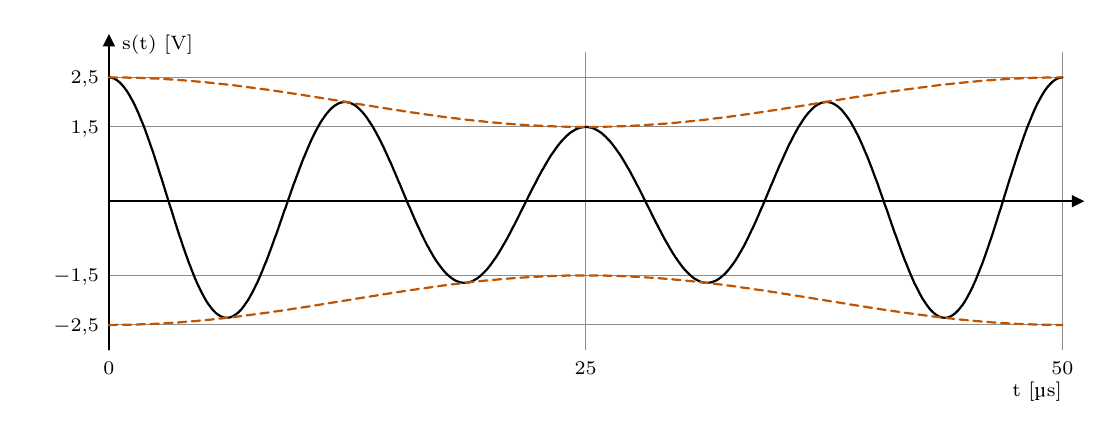
\begin{tikzpicture}[x=0.01985cm,y=-0.01985cm,line cap=round,line join=round]
\useasboundingbox (0,0) rectangle (680,240);
\path[draw=black!45,line width=0.35pt] (52,206) -- (52,16);
\path[draw=black!45,line width=0.35pt] (357,206) -- (357,16);
\path[draw=black!45,line width=0.35pt] (662,206) -- (662,16);
\path[draw=black!45,line width=0.35pt] (52,31.8) -- (662,31.8);
\path[draw=black!45,line width=0.35pt] (52,63.5) -- (662,63.5);
\path[draw=black!45,line width=0.35pt] (52,158.5) -- (662,158.5);
\path[draw=black!45,line width=0.35pt] (52,190.2) -- (662,190.2);
\path[draw=black,line width=0.7pt] (52,111) -- (670,111);
\path[fill=black,draw=none] (676,111) -- (668,107) -- (668,115) -- cycle;
\path[draw=black,line width=0.7pt] (52,206) -- (52,10);
\path[fill=black,draw=none] (52,4) -- (48,12) -- (56,12) -- cycle;
\node[anchor=base,inner sep=0pt,font=\scriptsize] at (52,222) {0};
\node[anchor=base,inner sep=0pt,font=\scriptsize] at (357,222) {25};
\node[anchor=base,inner sep=0pt,font=\scriptsize] at (662,222) {50};
\node[anchor=base east,inner sep=0pt,font=\scriptsize] at (46,35.8) {2,5};
\node[anchor=base east,inner sep=0pt,font=\scriptsize] at (46,67.5) {1,5};
\node[anchor=base east,inner sep=0pt,font=\scriptsize] at (46,162.5) {$-$1,5};
\node[anchor=base east,inner sep=0pt,font=\scriptsize] at (46,194.2) {$-$2,5};
\node[anchor=base east,inner sep=0pt,font=\scriptsize] at (662,236) {t [\textmu{}s]};
\node[anchor=base west,inner sep=0pt,font=\scriptsize] at (60,14) {s(t) [V]};
\path[draw=black,line width=0.8pt] (52,31.8) -- (52.5,31.9) -- (53,31.9) -- (53.5,32) -- (54,32.1) -- (54.5,32.3) -- (55.1,32.5) -- (55.6,32.7) -- (56.1,33) -- (56.6,33.3) -- (57.1,33.6) -- (57.6,34) -- (58.1,34.4) -- (58.6,34.8) -- (59.1,35.3) -- (59.6,35.8) -- (60.1,36.3) -- (60.6,36.9) -- (61.2,37.5) -- (61.7,38.1) -- (62.2,38.8) -- (62.7,39.5) -- (63.2,40.2) -- (63.7,40.9) -- (64.2,41.7) -- (64.7,42.6) -- (65.2,43.4) -- (65.7,44.3) -- (66.2,45.2) -- (66.7,46.1) -- (67.3,47.1) -- (67.8,48.1) -- (68.3,49.1) -- (68.8,50.2) -- (69.3,51.3) -- (69.8,52.4) -- (70.3,53.5) -- (70.8,54.6) -- (71.3,55.8) -- (71.8,57) -- (72.3,58.3) -- (72.8,59.5) -- (73.4,60.8) -- (73.9,62.1) -- (74.4,63.4) -- (74.9,64.7) -- (75.4,66.1) -- (75.9,67.5) -- (76.4,68.8) -- (76.9,70.3) -- (77.4,71.7) -- (77.9,73.1) -- (78.4,74.6) -- (78.9,76.1) -- (79.5,77.6) -- (80,79.1) -- (80.5,80.6) -- (81,82.1) -- (81.5,83.7) -- (82,85.2) -- (82.5,86.8) -- (83,88.3) -- (83.5,89.9) -- (84,91.5) -- (84.5,93.1) -- (85,94.7) -- (85.6,96.3) -- (86.1,98) -- (86.6,99.6) -- (87.1,101.2) -- (87.6,102.8) -- (88.1,104.5) -- (88.6,106.1) -- (89.1,107.7) -- (89.6,109.4) -- (90.1,111) -- (90.6,112.6) -- (91.1,114.3) -- (91.7,115.9) -- (92.2,117.5) -- (92.7,119.1) -- (93.2,120.7) -- (93.7,122.4) -- (94.2,124) -- (94.7,125.6) -- (95.2,127.1) -- (95.7,128.7) -- (96.2,130.3) -- (96.7,131.8) -- (97.2,133.4) -- (97.8,134.9) -- (98.3,136.5) -- (98.8,138) -- (99.3,139.5) -- (99.8,141) -- (100.3,142.4) -- (100.8,143.9) -- (101.3,145.3) -- (101.8,146.7) -- (102.3,148.1) -- (102.8,149.5) -- (103.3,150.9) -- (103.9,152.2) -- (104.4,153.6) -- (104.9,154.9) -- (105.4,156.2) -- (105.9,157.4) -- (106.4,158.7) -- (106.9,159.9) -- (107.4,161.1) -- (107.9,162.3) -- (108.4,163.4) -- (108.9,164.5) -- (109.4,165.6) -- (110,166.7) -- (110.5,167.8) -- (111,168.8) -- (111.5,169.8) -- (112,170.7) -- (112.5,171.7) -- (113,172.6) -- (113.5,173.5) -- (114,174.3) -- (114.5,175.2) -- (115,176) -- (115.5,176.7) -- (116.1,177.5) -- (116.6,178.2) -- (117.1,178.8) -- (117.6,179.5) -- (118.1,180.1) -- (118.6,180.7) -- (119.1,181.2) -- (119.6,181.7) -- (120.1,182.2) -- (120.6,182.7) -- (121.1,183.1) -- (121.6,183.5) -- (122.2,183.8) -- (122.7,184.2) -- (123.2,184.5) -- (123.7,184.7) -- (124.2,184.9) -- (124.7,185.1) -- (125.2,185.3) -- (125.7,185.4) -- (126.2,185.5) -- (126.7,185.6) -- (127.2,185.6) -- (127.7,185.6) -- (128.3,185.5) -- (128.8,185.5) -- (129.3,185.3) -- (129.8,185.2) -- (130.3,185) -- (130.8,184.8) -- (131.3,184.6) -- (131.8,184.3) -- (132.3,184) -- (132.8,183.7) -- (133.3,183.3) -- (133.8,182.9) -- (134.4,182.5) -- (134.9,182) -- (135.4,181.5) -- (135.9,181) -- (136.4,180.5) -- (136.9,179.9) -- (137.4,179.3) -- (137.9,178.6) -- (138.4,178) -- (138.9,177.3) -- (139.4,176.5) -- (139.9,175.8) -- (140.5,175) -- (141,174.2) -- (141.5,173.4) -- (142,172.5) -- (142.5,171.6) -- (143,170.7) -- (143.5,169.8) -- (144,168.8) -- (144.5,167.8) -- (145,166.8) -- (145.5,165.8) -- (146,164.7) -- (146.6,163.7) -- (147.1,162.6) -- (147.6,161.4) -- (148.1,160.3) -- (148.6,159.1) -- (149.1,158) -- (149.6,156.8) -- (150.1,155.6) -- (150.6,154.3) -- (151.1,153.1) -- (151.6,151.8) -- (152.1,150.5) -- (152.7,149.3) -- (153.2,147.9) -- (153.7,146.6) -- (154.2,145.3) -- (154.7,143.9) -- (155.2,142.6) -- (155.7,141.2) -- (156.2,139.8) -- (156.7,138.4) -- (157.2,137) -- (157.7,135.6) -- (158.2,134.2) -- (158.8,132.8) -- (159.3,131.4) -- (159.8,129.9) -- (160.3,128.5) -- (160.8,127) -- (161.3,125.6) -- (161.8,124.1) -- (162.3,122.7) -- (162.8,121.2) -- (163.3,119.8) -- (163.8,118.3) -- (164.3,116.8) -- (164.9,115.4) -- (165.4,113.9) -- (165.9,112.5) -- (166.4,111) -- (166.9,109.5) -- (167.4,108.1) -- (167.9,106.7) -- (168.4,105.2) -- (168.9,103.8) -- (169.4,102.4) -- (169.9,100.9) -- (170.4,99.5) -- (171,98.1) -- (171.5,96.7) -- (172,95.3) -- (172.5,94) -- (173,92.6) -- (173.5,91.3) -- (174,89.9) -- (174.5,88.6) -- (175,87.3) -- (175.5,86) -- (176,84.7) -- (176.5,83.4) -- (177.1,82.2) -- (177.6,80.9) -- (178.1,79.7) -- (178.6,78.5) -- (179.1,77.3) -- (179.6,76.1) -- (180.1,75) -- (180.6,73.8) -- (181.1,72.7) -- (181.6,71.6) -- (182.1,70.5) -- (182.6,69.5) -- (183.2,68.4) -- (183.7,67.4) -- (184.2,66.4) -- (184.7,65.4) -- (185.2,64.5) -- (185.7,63.6) -- (186.2,62.7) -- (186.7,61.8) -- (187.2,60.9) -- (187.7,60.1) -- (188.2,59.3) -- (188.7,58.5) -- (189.3,57.8) -- (189.8,57) -- (190.3,56.3) -- (190.8,55.6) -- (191.3,55) -- (191.8,54.4) -- (192.3,53.8) -- (192.8,53.2) -- (193.3,52.6) -- (193.8,52.1) -- (194.3,51.6) -- (194.8,51.2) -- (195.4,50.7) -- (195.9,50.3) -- (196.4,49.9) -- (196.9,49.6) -- (197.4,49.3) -- (197.9,49) -- (198.4,48.7) -- (198.9,48.5) -- (199.4,48.2) -- (199.9,48.1) -- (200.4,47.9) -- (200.9,47.8) -- (201.5,47.7) -- (202,47.6) -- (202.5,47.6) -- (203,47.5) -- (203.5,47.6) -- (204,47.6) -- (204.5,47.7) -- (205,47.8) -- (205.5,47.9) -- (206,48) -- (206.5,48.2) -- (207,48.4) -- (207.6,48.7) -- (208.1,48.9) -- (208.6,49.2) -- (209.1,49.5) -- (209.6,49.9) -- (210.1,50.2) -- (210.6,50.6) -- (211.1,51) -- (211.6,51.5) -- (212.1,51.9) -- (212.6,52.4) -- (213.1,53) -- (213.7,53.5) -- (214.2,54.1) -- (214.7,54.7) -- (215.2,55.3) -- (215.7,55.9) -- (216.2,56.6) -- (216.7,57.2) -- (217.2,57.9) -- (217.7,58.7) -- (218.2,59.4) -- (218.7,60.2) -- (219.2,61) -- (219.8,61.8) -- (220.3,62.6) -- (220.8,63.4) -- (221.3,64.3) -- (221.8,65.2) -- (222.3,66.1) -- (222.8,67) -- (223.3,67.9) -- (223.8,68.9) -- (224.3,69.8) -- (224.8,70.8) -- (225.3,71.8) -- (225.9,72.8) -- (226.4,73.9) -- (226.9,74.9) -- (227.4,75.9) -- (227.9,77) -- (228.4,78.1) -- (228.9,79.2) -- (229.4,80.3) -- (229.9,81.4) -- (230.4,82.5) -- (230.9,83.6) -- (231.4,84.8) -- (232,85.9) -- (232.5,87.1) -- (233,88.2) -- (233.5,89.4) -- (234,90.6) -- (234.5,91.8) -- (235,92.9) -- (235.5,94.1) -- (236,95.3) -- (236.5,96.5) -- (237,97.7) -- (237.5,98.9) -- (238.1,100.1) -- (238.6,101.3) -- (239.1,102.6) -- (239.6,103.8) -- (240.1,105) -- (240.6,106.2) -- (241.1,107.4) -- (241.6,108.6) -- (242.1,109.8) -- (242.6,111) -- (243.1,112.2) -- (243.6,113.4) -- (244.2,114.6) -- (244.7,115.8) -- (245.2,116.9) -- (245.7,118.1) -- (246.2,119.3) -- (246.7,120.5) -- (247.2,121.6) -- (247.7,122.8) -- (248.2,123.9) -- (248.7,125) -- (249.2,126.1) -- (249.7,127.2) -- (250.3,128.3) -- (250.8,129.4) -- (251.3,130.5) -- (251.8,131.6) -- (252.3,132.6) -- (252.8,133.7) -- (253.3,134.7) -- (253.8,135.7) -- (254.3,136.7) -- (254.8,137.7) -- (255.3,138.7) -- (255.8,139.7) -- (256.4,140.6) -- (256.9,141.5) -- (257.4,142.5) -- (257.9,143.4) -- (258.4,144.2) -- (258.9,145.1) -- (259.4,146) -- (259.9,146.8) -- (260.4,147.6) -- (260.9,148.4) -- (261.4,149.2) -- (261.9,149.9) -- (262.5,150.7) -- (263,151.4) -- (263.5,152.1) -- (264,152.8) -- (264.5,153.4) -- (265,154.1) -- (265.5,154.7) -- (266,155.3) -- (266.5,155.9) -- (267,156.4) -- (267.5,157) -- (268,157.5) -- (268.5,158) -- (269.1,158.5) -- (269.6,158.9) -- (270.1,159.3) -- (270.6,159.8) -- (271.1,160.1) -- (271.6,160.5) -- (272.1,160.8) -- (272.6,161.2) -- (273.1,161.5) -- (273.6,161.7) -- (274.1,162) -- (274.7,162.2) -- (275.2,162.4) -- (275.7,162.6) -- (276.2,162.7) -- (276.7,162.9) -- (277.2,163) -- (277.7,163.1) -- (278.2,163.1) -- (278.7,163.2) -- (279.2,163.2) -- (279.7,163.2) -- (280.2,163.2) -- (280.8,163.1) -- (281.3,163.1) -- (281.8,163) -- (282.3,162.9) -- (282.8,162.7) -- (283.3,162.6) -- (283.8,162.4) -- (284.3,162.2) -- (284.8,162) -- (285.3,161.7) -- (285.8,161.4) -- (286.3,161.2) -- (286.9,160.8) -- (287.4,160.5) -- (287.9,160.2) -- (288.4,159.8) -- (288.9,159.4) -- (289.4,159) -- (289.9,158.5) -- (290.4,158.1) -- (290.9,157.6) -- (291.4,157.1) -- (291.9,156.6) -- (292.4,156.1) -- (293,155.5) -- (293.5,155) -- (294,154.4) -- (294.5,153.8) -- (295,153.2) -- (295.5,152.5) -- (296,151.9) -- (296.5,151.2) -- (297,150.5) -- (297.5,149.8) -- (298,149.1) -- (298.5,148.4) -- (299.1,147.6) -- (299.6,146.9) -- (300.1,146.1) -- (300.6,145.3) -- (301.1,144.5) -- (301.6,143.7) -- (302.1,142.8) -- (302.6,142) -- (303.1,141.2) -- (303.6,140.3) -- (304.1,139.4) -- (304.6,138.5) -- (305.2,137.6) -- (305.7,136.7) -- (306.2,135.8) -- (306.7,134.9) -- (307.2,134) -- (307.7,133) -- (308.2,132.1) -- (308.7,131.1) -- (309.2,130.1) -- (309.7,129.2) -- (310.2,128.2) -- (310.7,127.2) -- (311.3,126.2) -- (311.8,125.2) -- (312.3,124.2) -- (312.8,123.2) -- (313.3,122.2) -- (313.8,121.2) -- (314.3,120.2) -- (314.8,119.2) -- (315.3,118.1) -- (315.8,117.1) -- (316.3,116.1) -- (316.8,115.1) -- (317.4,114.1) -- (317.9,113) -- (318.4,112) -- (318.9,111) -- (319.4,110) -- (319.9,109) -- (320.4,107.9) -- (320.9,106.9) -- (321.4,105.9) -- (321.9,104.9) -- (322.4,103.9) -- (322.9,102.9) -- (323.5,101.9) -- (324,100.9) -- (324.5,100) -- (325,99) -- (325.5,98) -- (326,97) -- (326.5,96.1) -- (327,95.1) -- (327.5,94.2) -- (328,93.3) -- (328.5,92.3) -- (329,91.4) -- (329.6,90.5) -- (330.1,89.6) -- (330.6,88.7) -- (331.1,87.8) -- (331.6,87) -- (332.1,86.1) -- (332.6,85.3) -- (333.1,84.4) -- (333.6,83.6) -- (334.1,82.8) -- (334.6,82) -- (335.1,81.2) -- (335.7,80.5) -- (336.2,79.7) -- (336.7,79) -- (337.2,78.3) -- (337.7,77.5) -- (338.2,76.9) -- (338.7,76.2) -- (339.2,75.5) -- (339.7,74.9) -- (340.2,74.2) -- (340.7,73.6) -- (341.2,73) -- (341.8,72.4) -- (342.3,71.8) -- (342.8,71.3) -- (343.3,70.8) -- (343.8,70.2) -- (344.3,69.7) -- (344.8,69.3) -- (345.3,68.8) -- (345.8,68.4) -- (346.3,67.9) -- (346.8,67.5) -- (347.3,67.1) -- (347.8,66.8) -- (348.4,66.4) -- (348.9,66.1) -- (349.4,65.8) -- (349.9,65.5) -- (350.4,65.2) -- (350.9,65) -- (351.4,64.7) -- (351.9,64.5) -- (352.4,64.3) -- (352.9,64.2) -- (353.4,64) -- (354,63.9) -- (354.5,63.8) -- (355,63.7) -- (355.5,63.6) -- (356,63.5) -- (356.5,63.5) -- (357,63.5) -- (357.5,63.5) -- (358,63.5) -- (358.5,63.6) -- (359,63.7) -- (359.5,63.8) -- (360.1,63.9) -- (360.6,64) -- (361.1,64.2) -- (361.6,64.3) -- (362.1,64.5) -- (362.6,64.7) -- (363.1,65) -- (363.6,65.2) -- (364.1,65.5) -- (364.6,65.8) -- (365.1,66.1) -- (365.6,66.4) -- (366.2,66.8) -- (366.7,67.1) -- (367.2,67.5) -- (367.7,67.9) -- (368.2,68.4) -- (368.7,68.8) -- (369.2,69.3) -- (369.7,69.7) -- (370.2,70.2) -- (370.7,70.8) -- (371.2,71.3) -- (371.7,71.8) -- (372.3,72.4) -- (372.8,73) -- (373.3,73.6) -- (373.8,74.2) -- (374.3,74.9) -- (374.8,75.5) -- (375.3,76.2) -- (375.8,76.9) -- (376.3,77.5) -- (376.8,78.3) -- (377.3,79) -- (377.8,79.7) -- (378.4,80.5) -- (378.9,81.2) -- (379.4,82) -- (379.9,82.8) -- (380.4,83.6) -- (380.9,84.4) -- (381.4,85.3) -- (381.9,86.1) -- (382.4,87) -- (382.9,87.8) -- (383.4,88.7) -- (383.9,89.6) -- (384.5,90.5) -- (385,91.4) -- (385.5,92.3) -- (386,93.3) -- (386.5,94.2) -- (387,95.1) -- (387.5,96.1) -- (388,97) -- (388.5,98) -- (389,99) -- (389.5,100) -- (390,100.9) -- (390.6,101.9) -- (391.1,102.9) -- (391.6,103.9) -- (392.1,104.9) -- (392.6,105.9) -- (393.1,106.9) -- (393.6,107.9) -- (394.1,109) -- (394.6,110) -- (395.1,111) -- (395.6,112) -- (396.1,113) -- (396.7,114.1) -- (397.2,115.1) -- (397.7,116.1) -- (398.2,117.1) -- (398.7,118.1) -- (399.2,119.2) -- (399.7,120.2) -- (400.2,121.2) -- (400.7,122.2) -- (401.2,123.2) -- (401.7,124.2) -- (402.2,125.2) -- (402.8,126.2) -- (403.3,127.2) -- (403.8,128.2) -- (404.3,129.2) -- (404.8,130.1) -- (405.3,131.1) -- (405.8,132.1) -- (406.3,133) -- (406.8,134) -- (407.3,134.9) -- (407.8,135.8) -- (408.3,136.7) -- (408.8,137.6) -- (409.4,138.5) -- (409.9,139.4) -- (410.4,140.3) -- (410.9,141.2) -- (411.4,142) -- (411.9,142.8) -- (412.4,143.7) -- (412.9,144.5) -- (413.4,145.3) -- (413.9,146.1) -- (414.4,146.9) -- (415,147.6) -- (415.5,148.4) -- (416,149.1) -- (416.5,149.8) -- (417,150.5) -- (417.5,151.2) -- (418,151.9) -- (418.5,152.5) -- (419,153.2) -- (419.5,153.8) -- (420,154.4) -- (420.5,155) -- (421.1,155.5) -- (421.6,156.1) -- (422.1,156.6) -- (422.6,157.1) -- (423.1,157.6) -- (423.6,158.1) -- (424.1,158.5) -- (424.6,159) -- (425.1,159.4) -- (425.6,159.8) -- (426.1,160.2) -- (426.6,160.5) -- (427.2,160.8) -- (427.7,161.2) -- (428.2,161.4) -- (428.7,161.7) -- (429.2,162) -- (429.7,162.2) -- (430.2,162.4) -- (430.7,162.6) -- (431.2,162.7) -- (431.7,162.9) -- (432.2,163) -- (432.7,163.1) -- (433.3,163.1) -- (433.8,163.2) -- (434.3,163.2) -- (434.8,163.2) -- (435.3,163.2) -- (435.8,163.1) -- (436.3,163.1) -- (436.8,163) -- (437.3,162.9) -- (437.8,162.7) -- (438.3,162.6) -- (438.8,162.4) -- (439.4,162.2) -- (439.9,162) -- (440.4,161.7) -- (440.9,161.5) -- (441.4,161.2) -- (441.9,160.8) -- (442.4,160.5) -- (442.9,160.1) -- (443.4,159.8) -- (443.9,159.3) -- (444.4,158.9) -- (444.9,158.5) -- (445.5,158) -- (446,157.5) -- (446.5,157) -- (447,156.4) -- (447.5,155.9) -- (448,155.3) -- (448.5,154.7) -- (449,154.1) -- (449.5,153.4) -- (450,152.8) -- (450.5,152.1) -- (451,151.4) -- (451.6,150.7) -- (452.1,149.9) -- (452.6,149.2) -- (453.1,148.4) -- (453.6,147.6) -- (454.1,146.8) -- (454.6,146) -- (455.1,145.1) -- (455.6,144.2) -- (456.1,143.4) -- (456.6,142.5) -- (457.1,141.5) -- (457.7,140.6) -- (458.2,139.7) -- (458.7,138.7) -- (459.2,137.7) -- (459.7,136.7) -- (460.2,135.7) -- (460.7,134.7) -- (461.2,133.7) -- (461.7,132.6) -- (462.2,131.6) -- (462.7,130.5) -- (463.2,129.4) -- (463.8,128.3) -- (464.3,127.2) -- (464.8,126.1) -- (465.3,125) -- (465.8,123.9) -- (466.3,122.8) -- (466.8,121.6) -- (467.3,120.5) -- (467.8,119.3) -- (468.3,118.1) -- (468.8,116.9) -- (469.3,115.8) -- (469.9,114.6) -- (470.4,113.4) -- (470.9,112.2) -- (471.4,111) -- (471.9,109.8) -- (472.4,108.6) -- (472.9,107.4) -- (473.4,106.2) -- (473.9,105) -- (474.4,103.8) -- (474.9,102.6) -- (475.4,101.3) -- (476,100.1) -- (476.5,98.9) -- (477,97.7) -- (477.5,96.5) -- (478,95.3) -- (478.5,94.1) -- (479,92.9) -- (479.5,91.8) -- (480,90.6) -- (480.5,89.4) -- (481,88.2) -- (481.5,87.1) -- (482.1,85.9) -- (482.6,84.8) -- (483.1,83.6) -- (483.6,82.5) -- (484.1,81.4) -- (484.6,80.3) -- (485.1,79.2) -- (485.6,78.1) -- (486.1,77) -- (486.6,75.9) -- (487.1,74.9) -- (487.6,73.9) -- (488.2,72.8) -- (488.7,71.8) -- (489.2,70.8) -- (489.7,69.8) -- (490.2,68.9) -- (490.7,67.9) -- (491.2,67) -- (491.7,66.1) -- (492.2,65.2) -- (492.7,64.3) -- (493.2,63.4) -- (493.7,62.6) -- (494.3,61.8) -- (494.8,61) -- (495.3,60.2) -- (495.8,59.4) -- (496.3,58.7) -- (496.8,57.9) -- (497.3,57.2) -- (497.8,56.6) -- (498.3,55.9) -- (498.8,55.3) -- (499.3,54.7) -- (499.8,54.1) -- (500.4,53.5) -- (500.9,53) -- (501.4,52.4) -- (501.9,51.9) -- (502.4,51.5) -- (502.9,51) -- (503.4,50.6) -- (503.9,50.2) -- (504.4,49.9) -- (504.9,49.5) -- (505.4,49.2) -- (505.9,48.9) -- (506.5,48.7) -- (507,48.4) -- (507.5,48.2) -- (508,48) -- (508.5,47.9) -- (509,47.8) -- (509.5,47.7) -- (510,47.6) -- (510.5,47.6) -- (511,47.5) -- (511.5,47.6) -- (512,47.6) -- (512.6,47.7) -- (513.1,47.8) -- (513.6,47.9) -- (514.1,48.1) -- (514.6,48.2) -- (515.1,48.5) -- (515.6,48.7) -- (516.1,49) -- (516.6,49.3) -- (517.1,49.6) -- (517.6,49.9) -- (518.1,50.3) -- (518.7,50.7) -- (519.2,51.2) -- (519.7,51.6) -- (520.2,52.1) -- (520.7,52.6) -- (521.2,53.2) -- (521.7,53.8) -- (522.2,54.4) -- (522.7,55) -- (523.2,55.6) -- (523.7,56.3) -- (524.2,57) -- (524.8,57.8) -- (525.3,58.5) -- (525.8,59.3) -- (526.3,60.1) -- (526.8,60.9) -- (527.3,61.8) -- (527.8,62.7) -- (528.3,63.6) -- (528.8,64.5) -- (529.3,65.4) -- (529.8,66.4) -- (530.3,67.4) -- (530.9,68.4) -- (531.4,69.5) -- (531.9,70.5) -- (532.4,71.6) -- (532.9,72.7) -- (533.4,73.8) -- (533.9,75) -- (534.4,76.1) -- (534.9,77.3) -- (535.4,78.5) -- (535.9,79.7) -- (536.4,80.9) -- (537,82.2) -- (537.5,83.4) -- (538,84.7) -- (538.5,86) -- (539,87.3) -- (539.5,88.6) -- (540,89.9) -- (540.5,91.3) -- (541,92.6) -- (541.5,94) -- (542,95.3) -- (542.5,96.7) -- (543.1,98.1) -- (543.6,99.5) -- (544.1,100.9) -- (544.6,102.4) -- (545.1,103.8) -- (545.6,105.2) -- (546.1,106.7) -- (546.6,108.1) -- (547.1,109.5) -- (547.6,111) -- (548.1,112.5) -- (548.6,113.9) -- (549.2,115.4) -- (549.7,116.8) -- (550.2,118.3) -- (550.7,119.8) -- (551.2,121.2) -- (551.7,122.7) -- (552.2,124.1) -- (552.7,125.6) -- (553.2,127) -- (553.7,128.5) -- (554.2,129.9) -- (554.7,131.4) -- (555.3,132.8) -- (555.8,134.2) -- (556.3,135.6) -- (556.8,137) -- (557.3,138.4) -- (557.8,139.8) -- (558.3,141.2) -- (558.8,142.6) -- (559.3,143.9) -- (559.8,145.3) -- (560.3,146.6) -- (560.8,147.9) -- (561.3,149.3) -- (561.9,150.5) -- (562.4,151.8) -- (562.9,153.1) -- (563.4,154.3) -- (563.9,155.6) -- (564.4,156.8) -- (564.9,158) -- (565.4,159.1) -- (565.9,160.3) -- (566.4,161.4) -- (566.9,162.6) -- (567.4,163.7) -- (568,164.7) -- (568.5,165.8) -- (569,166.8) -- (569.5,167.8) -- (570,168.8) -- (570.5,169.8) -- (571,170.7) -- (571.5,171.6) -- (572,172.5) -- (572.5,173.4) -- (573,174.2) -- (573.6,175) -- (574.1,175.8) -- (574.6,176.5) -- (575.1,177.3) -- (575.6,178) -- (576.1,178.6) -- (576.6,179.3) -- (577.1,179.9) -- (577.6,180.5) -- (578.1,181) -- (578.6,181.5) -- (579.1,182) -- (579.7,182.5) -- (580.2,182.9) -- (580.7,183.3) -- (581.2,183.7) -- (581.7,184) -- (582.2,184.3) -- (582.7,184.6) -- (583.2,184.8) -- (583.7,185) -- (584.2,185.2) -- (584.7,185.3) -- (585.2,185.5) -- (585.8,185.5) -- (586.3,185.6) -- (586.8,185.6) -- (587.3,185.6) -- (587.8,185.5) -- (588.3,185.4) -- (588.8,185.3) -- (589.3,185.1) -- (589.8,184.9) -- (590.3,184.7) -- (590.8,184.5) -- (591.3,184.2) -- (591.9,183.8) -- (592.4,183.5) -- (592.9,183.1) -- (593.4,182.7) -- (593.9,182.2) -- (594.4,181.7) -- (594.9,181.2) -- (595.4,180.7) -- (595.9,180.1) -- (596.4,179.5) -- (596.9,178.8) -- (597.4,178.2) -- (598,177.5) -- (598.5,176.7) -- (599,176) -- (599.5,175.2) -- (600,174.3) -- (600.5,173.5) -- (601,172.6) -- (601.5,171.7) -- (602,170.7) -- (602.5,169.8) -- (603,168.8) -- (603.5,167.8) -- (604.1,166.7) -- (604.6,165.6) -- (605.1,164.5) -- (605.6,163.4) -- (606.1,162.3) -- (606.6,161.1) -- (607.1,159.9) -- (607.6,158.7) -- (608.1,157.4) -- (608.6,156.2) -- (609.1,154.9) -- (609.6,153.6) -- (610.2,152.2) -- (610.7,150.9) -- (611.2,149.5) -- (611.7,148.1) -- (612.2,146.7) -- (612.7,145.3) -- (613.2,143.9) -- (613.7,142.4) -- (614.2,141) -- (614.7,139.5) -- (615.2,138) -- (615.7,136.5) -- (616.3,134.9) -- (616.8,133.4) -- (617.3,131.8) -- (617.8,130.3) -- (618.3,128.7) -- (618.8,127.1) -- (619.3,125.6) -- (619.8,124) -- (620.3,122.4) -- (620.8,120.7) -- (621.3,119.1) -- (621.8,117.5) -- (622.4,115.9) -- (622.9,114.3) -- (623.4,112.6) -- (623.9,111) -- (624.4,109.4) -- (624.9,107.7) -- (625.4,106.1) -- (625.9,104.5) -- (626.4,102.8) -- (626.9,101.2) -- (627.4,99.6) -- (627.9,98) -- (628.4,96.3) -- (629,94.7) -- (629.5,93.1) -- (630,91.5) -- (630.5,89.9) -- (631,88.3) -- (631.5,86.8) -- (632,85.2) -- (632.5,83.7) -- (633,82.1) -- (633.5,80.6) -- (634,79.1) -- (634.6,77.6) -- (635.1,76.1) -- (635.6,74.6) -- (636.1,73.1) -- (636.6,71.7) -- (637.1,70.3) -- (637.6,68.8) -- (638.1,67.5) -- (638.6,66.1) -- (639.1,64.7) -- (639.6,63.4) -- (640.1,62.1) -- (640.7,60.8) -- (641.2,59.5) -- (641.7,58.3) -- (642.2,57) -- (642.7,55.8) -- (643.2,54.6) -- (643.7,53.5) -- (644.2,52.4) -- (644.7,51.3) -- (645.2,50.2) -- (645.7,49.1) -- (646.2,48.1) -- (646.8,47.1) -- (647.3,46.1) -- (647.8,45.2) -- (648.3,44.3) -- (648.8,43.4) -- (649.3,42.6) -- (649.8,41.7) -- (650.3,40.9) -- (650.8,40.2) -- (651.3,39.5) -- (651.8,38.8) -- (652.3,38.1) -- (652.9,37.5) -- (653.4,36.9) -- (653.9,36.3) -- (654.4,35.8) -- (654.9,35.3) -- (655.4,34.8) -- (655.9,34.4) -- (656.4,34) -- (656.9,33.6) -- (657.4,33.3) -- (657.9,33) -- (658.4,32.7) -- (659,32.5) -- (659.5,32.3) -- (660,32.1) -- (660.5,32) -- (661,31.9) -- (661.5,31.9) -- (662,31.8);
\path[draw=cB,line width=0.8pt,dash pattern=on 3pt off 2pt] (52,31.8) -- (52.8,31.8) -- (53.5,31.8) -- (54.3,31.8) -- (55.1,31.8) -- (55.8,31.8) -- (56.6,31.9) -- (57.3,31.9) -- (58.1,31.9) -- (58.9,31.9) -- (59.6,31.9) -- (60.4,31.9) -- (61.2,31.9) -- (61.9,31.9) -- (62.7,31.9) -- (63.4,31.9) -- (64.2,32) -- (65,32) -- (65.7,32) -- (66.5,32) -- (67.3,32) -- (68,32) -- (68.8,32.1) -- (69.5,32.1) -- (70.3,32.1) -- (71.1,32.1) -- (71.8,32.2) -- (72.6,32.2) -- (73.4,32.2) -- (74.1,32.2) -- (74.9,32.3) -- (75.6,32.3) -- (76.4,32.3) -- (77.2,32.4) -- (77.9,32.4) -- (78.7,32.4) -- (79.5,32.5) -- (80.2,32.5) -- (81,32.5) -- (81.7,32.6) -- (82.5,32.6) -- (83.3,32.6) -- (84,32.7) -- (84.8,32.7) -- (85.6,32.8) -- (86.3,32.8) -- (87.1,32.9) -- (87.8,32.9) -- (88.6,32.9) -- (89.4,33) -- (90.1,33) -- (90.9,33.1) -- (91.7,33.1) -- (92.4,33.2) -- (93.2,33.2) -- (93.9,33.3) -- (94.7,33.3) -- (95.5,33.4) -- (96.2,33.4) -- (97,33.5) -- (97.8,33.6) -- (98.5,33.6) -- (99.3,33.7) -- (100,33.7) -- (100.8,33.8) -- (101.6,33.9) -- (102.3,33.9) -- (103.1,34) -- (103.9,34) -- (104.6,34.1) -- (105.4,34.2) -- (106.1,34.2) -- (106.9,34.3) -- (107.7,34.4) -- (108.4,34.4) -- (109.2,34.5) -- (110,34.6) -- (110.7,34.6) -- (111.5,34.7) -- (112.2,34.8) -- (113,34.9) -- (113.8,34.9) -- (114.5,35) -- (115.3,35.1) -- (116.1,35.2) -- (116.8,35.2) -- (117.6,35.3) -- (118.3,35.4) -- (119.1,35.5) -- (119.9,35.5) -- (120.6,35.6) -- (121.4,35.7) -- (122.2,35.8) -- (122.9,35.9) -- (123.7,36) -- (124.4,36) -- (125.2,36.1) -- (126,36.2) -- (126.7,36.3) -- (127.5,36.4) -- (128.3,36.5) -- (129,36.6) -- (129.8,36.6) -- (130.5,36.7) -- (131.3,36.8) -- (132.1,36.9) -- (132.8,37) -- (133.6,37.1) -- (134.4,37.2) -- (135.1,37.3) -- (135.9,37.4) -- (136.6,37.5) -- (137.4,37.6) -- (138.2,37.7) -- (138.9,37.8) -- (139.7,37.9) -- (140.5,38) -- (141.2,38.1) -- (142,38.2) -- (142.7,38.3) -- (143.5,38.4) -- (144.3,38.5) -- (145,38.6) -- (145.8,38.7) -- (146.6,38.8) -- (147.3,38.9) -- (148.1,39) -- (148.8,39.1) -- (149.6,39.2) -- (150.4,39.3) -- (151.1,39.4) -- (151.9,39.5) -- (152.7,39.6) -- (153.4,39.7) -- (154.2,39.8) -- (154.9,39.9) -- (155.7,40) -- (156.5,40.1) -- (157.2,40.3) -- (158,40.4) -- (158.8,40.5) -- (159.5,40.6) -- (160.3,40.7) -- (161,40.8) -- (161.8,40.9) -- (162.6,41) -- (163.3,41.2) -- (164.1,41.3) -- (164.9,41.4) -- (165.6,41.5) -- (166.4,41.6) -- (167.1,41.7) -- (167.9,41.8) -- (168.7,42) -- (169.4,42.1) -- (170.2,42.2) -- (171,42.3) -- (171.7,42.4) -- (172.5,42.5) -- (173.2,42.7) -- (174,42.8) -- (174.8,42.9) -- (175.5,43) -- (176.3,43.1) -- (177.1,43.2) -- (177.8,43.4) -- (178.6,43.5) -- (179.3,43.6) -- (180.1,43.7) -- (180.9,43.8) -- (181.6,44) -- (182.4,44.1) -- (183.2,44.2) -- (183.9,44.3) -- (184.7,44.5) -- (185.4,44.6) -- (186.2,44.7) -- (187,44.8) -- (187.7,44.9) -- (188.5,45.1) -- (189.3,45.2) -- (190,45.3) -- (190.8,45.4) -- (191.5,45.6) -- (192.3,45.7) -- (193.1,45.8) -- (193.8,45.9) -- (194.6,46.1) -- (195.4,46.2) -- (196.1,46.3) -- (196.9,46.4) -- (197.6,46.5) -- (198.4,46.7) -- (199.2,46.8) -- (199.9,46.9) -- (200.7,47) -- (201.5,47.2) -- (202.2,47.3) -- (203,47.4) -- (203.7,47.5) -- (204.5,47.7) -- (205.3,47.8) -- (206,47.9) -- (206.8,48) -- (207.6,48.2) -- (208.3,48.3) -- (209.1,48.4) -- (209.8,48.5) -- (210.6,48.7) -- (211.4,48.8) -- (212.1,48.9) -- (212.9,49) -- (213.7,49.2) -- (214.4,49.3) -- (215.2,49.4) -- (215.9,49.5) -- (216.7,49.7) -- (217.5,49.8) -- (218.2,49.9) -- (219,50) -- (219.8,50.1) -- (220.5,50.3) -- (221.3,50.4) -- (222,50.5) -- (222.8,50.6) -- (223.6,50.8) -- (224.3,50.9) -- (225.1,51) -- (225.9,51.1) -- (226.6,51.2) -- (227.4,51.4) -- (228.1,51.5) -- (228.9,51.6) -- (229.7,51.7) -- (230.4,51.8) -- (231.2,52) -- (232,52.1) -- (232.7,52.2) -- (233.5,52.3) -- (234.2,52.4) -- (235,52.6) -- (235.8,52.7) -- (236.5,52.8) -- (237.3,52.9) -- (238.1,53) -- (238.8,53.1) -- (239.6,53.3) -- (240.3,53.4) -- (241.1,53.5) -- (241.9,53.6) -- (242.6,53.7) -- (243.4,53.8) -- (244.2,54) -- (244.9,54.1) -- (245.7,54.2) -- (246.4,54.3) -- (247.2,54.4) -- (248,54.5) -- (248.7,54.6) -- (249.5,54.7) -- (250.3,54.9) -- (251,55) -- (251.8,55.1) -- (252.5,55.2) -- (253.3,55.3) -- (254.1,55.4) -- (254.8,55.5) -- (255.6,55.6) -- (256.4,55.7) -- (257.1,55.8) -- (257.9,55.9) -- (258.6,56) -- (259.4,56.2) -- (260.2,56.3) -- (260.9,56.4) -- (261.7,56.5) -- (262.5,56.6) -- (263.2,56.7) -- (264,56.8) -- (264.7,56.9) -- (265.5,57) -- (266.3,57.1) -- (267,57.2) -- (267.8,57.3) -- (268.5,57.4) -- (269.3,57.5) -- (270.1,57.6) -- (270.8,57.7) -- (271.6,57.8) -- (272.4,57.9) -- (273.1,57.9) -- (273.9,58) -- (274.7,58.1) -- (275.4,58.2) -- (276.2,58.3) -- (276.9,58.4) -- (277.7,58.5) -- (278.5,58.6) -- (279.2,58.7) -- (280,58.8) -- (280.8,58.9) -- (281.5,59) -- (282.3,59) -- (283,59.1) -- (283.8,59.2) -- (284.6,59.3) -- (285.3,59.4) -- (286.1,59.5) -- (286.9,59.5) -- (287.6,59.6) -- (288.4,59.7) -- (289.1,59.8) -- (289.9,59.9) -- (290.7,59.9) -- (291.4,60) -- (292.2,60.1) -- (293,60.2) -- (293.7,60.3) -- (294.5,60.3) -- (295.2,60.4) -- (296,60.5) -- (296.8,60.5) -- (297.5,60.6) -- (298.3,60.7) -- (299.1,60.8) -- (299.8,60.8) -- (300.6,60.9) -- (301.3,61) -- (302.1,61) -- (302.9,61.1) -- (303.6,61.2) -- (304.4,61.2) -- (305.2,61.3) -- (305.9,61.4) -- (306.7,61.4) -- (307.4,61.5) -- (308.2,61.5) -- (309,61.6) -- (309.7,61.7) -- (310.5,61.7) -- (311.3,61.8) -- (312,61.8) -- (312.8,61.9) -- (313.5,61.9) -- (314.3,62) -- (315.1,62) -- (315.8,62.1) -- (316.6,62.1) -- (317.4,62.2) -- (318.1,62.2) -- (318.9,62.3) -- (319.6,62.3) -- (320.4,62.4) -- (321.2,62.4) -- (321.9,62.5) -- (322.7,62.5) -- (323.5,62.6) -- (324.2,62.6) -- (325,62.6) -- (325.7,62.7) -- (326.5,62.7) -- (327.3,62.8) -- (328,62.8) -- (328.8,62.8) -- (329.6,62.9) -- (330.3,62.9) -- (331.1,62.9) -- (331.8,63) -- (332.6,63) -- (333.4,63) -- (334.1,63.1) -- (334.9,63.1) -- (335.7,63.1) -- (336.4,63.1) -- (337.2,63.2) -- (337.9,63.2) -- (338.7,63.2) -- (339.5,63.2) -- (340.2,63.3) -- (341,63.3) -- (341.8,63.3) -- (342.5,63.3) -- (343.3,63.3) -- (344,63.4) -- (344.8,63.4) -- (345.6,63.4) -- (346.3,63.4) -- (347.1,63.4) -- (347.8,63.4) -- (348.6,63.4) -- (349.4,63.5) -- (350.1,63.5) -- (350.9,63.5) -- (351.7,63.5) -- (352.4,63.5) -- (353.2,63.5) -- (354,63.5) -- (354.7,63.5) -- (355.5,63.5) -- (356.2,63.5) -- (357,63.5) -- (357.8,63.5) -- (358.5,63.5) -- (359.3,63.5) -- (360.1,63.5) -- (360.8,63.5) -- (361.6,63.5) -- (362.3,63.5) -- (363.1,63.5) -- (363.9,63.5) -- (364.6,63.5) -- (365.4,63.4) -- (366.2,63.4) -- (366.9,63.4) -- (367.7,63.4) -- (368.4,63.4) -- (369.2,63.4) -- (370,63.4) -- (370.7,63.3) -- (371.5,63.3) -- (372.3,63.3) -- (373,63.3) -- (373.8,63.3) -- (374.5,63.2) -- (375.3,63.2) -- (376.1,63.2) -- (376.8,63.2) -- (377.6,63.1) -- (378.4,63.1) -- (379.1,63.1) -- (379.9,63.1) -- (380.6,63) -- (381.4,63) -- (382.2,63) -- (382.9,62.9) -- (383.7,62.9) -- (384.5,62.9) -- (385.2,62.8) -- (386,62.8) -- (386.7,62.8) -- (387.5,62.7) -- (388.3,62.7) -- (389,62.6) -- (389.8,62.6) -- (390.6,62.6) -- (391.3,62.5) -- (392.1,62.5) -- (392.8,62.4) -- (393.6,62.4) -- (394.4,62.3) -- (395.1,62.3) -- (395.9,62.2) -- (396.7,62.2) -- (397.4,62.1) -- (398.2,62.1) -- (398.9,62) -- (399.7,62) -- (400.5,61.9) -- (401.2,61.9) -- (402,61.8) -- (402.8,61.8) -- (403.5,61.7) -- (404.3,61.7) -- (405,61.6) -- (405.8,61.5) -- (406.6,61.5) -- (407.3,61.4) -- (408.1,61.4) -- (408.8,61.3) -- (409.6,61.2) -- (410.4,61.2) -- (411.1,61.1) -- (411.9,61) -- (412.7,61) -- (413.4,60.9) -- (414.2,60.8) -- (415,60.8) -- (415.7,60.7) -- (416.5,60.6) -- (417.2,60.5) -- (418,60.5) -- (418.8,60.4) -- (419.5,60.3) -- (420.3,60.3) -- (421.1,60.2) -- (421.8,60.1) -- (422.6,60) -- (423.3,59.9) -- (424.1,59.9) -- (424.9,59.8) -- (425.6,59.7) -- (426.4,59.6) -- (427.2,59.5) -- (427.9,59.5) -- (428.7,59.4) -- (429.4,59.3) -- (430.2,59.2) -- (431,59.1) -- (431.7,59) -- (432.5,59) -- (433.3,58.9) -- (434,58.8) -- (434.8,58.7) -- (435.5,58.6) -- (436.3,58.5) -- (437.1,58.4) -- (437.8,58.3) -- (438.6,58.2) -- (439.4,58.1) -- (440.1,58) -- (440.9,57.9) -- (441.6,57.9) -- (442.4,57.8) -- (443.2,57.7) -- (443.9,57.6) -- (444.7,57.5) -- (445.5,57.4) -- (446.2,57.3) -- (447,57.2) -- (447.7,57.1) -- (448.5,57) -- (449.3,56.9) -- (450,56.8) -- (450.8,56.7) -- (451.6,56.6) -- (452.3,56.5) -- (453.1,56.4) -- (453.8,56.3) -- (454.6,56.2) -- (455.4,56) -- (456.1,55.9) -- (456.9,55.8) -- (457.7,55.7) -- (458.4,55.6) -- (459.2,55.5) -- (459.9,55.4) -- (460.7,55.3) -- (461.5,55.2) -- (462.2,55.1) -- (463,55) -- (463.8,54.9) -- (464.5,54.7) -- (465.3,54.6) -- (466,54.5) -- (466.8,54.4) -- (467.6,54.3) -- (468.3,54.2) -- (469.1,54.1) -- (469.9,54) -- (470.6,53.8) -- (471.4,53.7) -- (472.1,53.6) -- (472.9,53.5) -- (473.7,53.4) -- (474.4,53.3) -- (475.2,53.1) -- (476,53) -- (476.7,52.9) -- (477.5,52.8) -- (478.2,52.7) -- (479,52.6) -- (479.8,52.4) -- (480.5,52.3) -- (481.3,52.2) -- (482.1,52.1) -- (482.8,52) -- (483.6,51.8) -- (484.3,51.7) -- (485.1,51.6) -- (485.9,51.5) -- (486.6,51.4) -- (487.4,51.2) -- (488.2,51.1) -- (488.9,51) -- (489.7,50.9) -- (490.4,50.8) -- (491.2,50.6) -- (492,50.5) -- (492.7,50.4) -- (493.5,50.3) -- (494.3,50.1) -- (495,50) -- (495.8,49.9) -- (496.5,49.8) -- (497.3,49.7) -- (498.1,49.5) -- (498.8,49.4) -- (499.6,49.3) -- (500.4,49.2) -- (501.1,49) -- (501.9,48.9) -- (502.6,48.8) -- (503.4,48.7) -- (504.2,48.5) -- (504.9,48.4) -- (505.7,48.3) -- (506.5,48.2) -- (507.2,48) -- (508,47.9) -- (508.7,47.8) -- (509.5,47.7) -- (510.3,47.5) -- (511,47.4) -- (511.8,47.3) -- (512.6,47.2) -- (513.3,47) -- (514.1,46.9) -- (514.8,46.8) -- (515.6,46.7) -- (516.4,46.5) -- (517.1,46.4) -- (517.9,46.3) -- (518.7,46.2) -- (519.4,46.1) -- (520.2,45.9) -- (520.9,45.8) -- (521.7,45.7) -- (522.5,45.6) -- (523.2,45.4) -- (524,45.3) -- (524.8,45.2) -- (525.5,45.1) -- (526.3,44.9) -- (527,44.8) -- (527.8,44.7) -- (528.6,44.6) -- (529.3,44.5) -- (530.1,44.3) -- (530.9,44.2) -- (531.6,44.1) -- (532.4,44) -- (533.1,43.8) -- (533.9,43.7) -- (534.7,43.6) -- (535.4,43.5) -- (536.2,43.4) -- (537,43.2) -- (537.7,43.1) -- (538.5,43) -- (539.2,42.9) -- (540,42.8) -- (540.8,42.7) -- (541.5,42.5) -- (542.3,42.4) -- (543.1,42.3) -- (543.8,42.2) -- (544.6,42.1) -- (545.3,42) -- (546.1,41.8) -- (546.9,41.7) -- (547.6,41.6) -- (548.4,41.5) -- (549.2,41.4) -- (549.9,41.3) -- (550.7,41.2) -- (551.4,41) -- (552.2,40.9) -- (553,40.8) -- (553.7,40.7) -- (554.5,40.6) -- (555.3,40.5) -- (556,40.4) -- (556.8,40.3) -- (557.5,40.1) -- (558.3,40) -- (559.1,39.9) -- (559.8,39.8) -- (560.6,39.7) -- (561.3,39.6) -- (562.1,39.5) -- (562.9,39.4) -- (563.6,39.3) -- (564.4,39.2) -- (565.2,39.1) -- (565.9,39) -- (566.7,38.9) -- (567.4,38.8) -- (568.2,38.7) -- (569,38.6) -- (569.7,38.5) -- (570.5,38.4) -- (571.3,38.3) -- (572,38.2) -- (572.8,38.1) -- (573.6,38) -- (574.3,37.9) -- (575.1,37.8) -- (575.8,37.7) -- (576.6,37.6) -- (577.4,37.5) -- (578.1,37.4) -- (578.9,37.3) -- (579.7,37.2) -- (580.4,37.1) -- (581.2,37) -- (581.9,36.9) -- (582.7,36.8) -- (583.5,36.7) -- (584.2,36.6) -- (585,36.6) -- (585.8,36.5) -- (586.5,36.4) -- (587.3,36.3) -- (588,36.2) -- (588.8,36.1) -- (589.6,36) -- (590.3,36) -- (591.1,35.9) -- (591.9,35.8) -- (592.6,35.7) -- (593.4,35.6) -- (594.1,35.5) -- (594.9,35.5) -- (595.7,35.4) -- (596.4,35.3) -- (597.2,35.2) -- (598,35.2) -- (598.7,35.1) -- (599.5,35) -- (600.2,34.9) -- (601,34.9) -- (601.8,34.8) -- (602.5,34.7) -- (603.3,34.6) -- (604.1,34.6) -- (604.8,34.5) -- (605.6,34.4) -- (606.3,34.4) -- (607.1,34.3) -- (607.9,34.2) -- (608.6,34.2) -- (609.4,34.1) -- (610.2,34) -- (610.9,34) -- (611.7,33.9) -- (612.4,33.9) -- (613.2,33.8) -- (614,33.7) -- (614.7,33.7) -- (615.5,33.6) -- (616.3,33.6) -- (617,33.5) -- (617.8,33.4) -- (618.5,33.4) -- (619.3,33.3) -- (620.1,33.3) -- (620.8,33.2) -- (621.6,33.2) -- (622.4,33.1) -- (623.1,33.1) -- (623.9,33) -- (624.6,33) -- (625.4,32.9) -- (626.2,32.9) -- (626.9,32.9) -- (627.7,32.8) -- (628.4,32.8) -- (629.2,32.7) -- (630,32.7) -- (630.7,32.6) -- (631.5,32.6) -- (632.3,32.6) -- (633,32.5) -- (633.8,32.5) -- (634.6,32.5) -- (635.3,32.4) -- (636.1,32.4) -- (636.8,32.4) -- (637.6,32.3) -- (638.4,32.3) -- (639.1,32.3) -- (639.9,32.2) -- (640.7,32.2) -- (641.4,32.2) -- (642.2,32.2) -- (642.9,32.1) -- (643.7,32.1) -- (644.5,32.1) -- (645.2,32.1) -- (646,32) -- (646.8,32) -- (647.5,32) -- (648.3,32) -- (649,32) -- (649.8,32) -- (650.6,31.9) -- (651.3,31.9) -- (652.1,31.9) -- (652.9,31.9) -- (653.6,31.9) -- (654.4,31.9) -- (655.1,31.9) -- (655.9,31.9) -- (656.7,31.9) -- (657.4,31.9) -- (658.2,31.8) -- (659,31.8) -- (659.7,31.8) -- (660.5,31.8) -- (661.2,31.8) -- (662,31.8);
\path[draw=cB,line width=0.8pt,dash pattern=on 3pt off 2pt] (52,190.2) -- (52.8,190.2) -- (53.5,190.2) -- (54.3,190.2) -- (55.1,190.2) -- (55.8,190.2) -- (56.6,190.1) -- (57.3,190.1) -- (58.1,190.1) -- (58.9,190.1) -- (59.6,190.1) -- (60.4,190.1) -- (61.2,190.1) -- (61.9,190.1) -- (62.7,190.1) -- (63.4,190.1) -- (64.2,190) -- (65,190) -- (65.7,190) -- (66.5,190) -- (67.3,190) -- (68,190) -- (68.8,189.9) -- (69.5,189.9) -- (70.3,189.9) -- (71.1,189.9) -- (71.8,189.8) -- (72.6,189.8) -- (73.4,189.8) -- (74.1,189.8) -- (74.9,189.7) -- (75.6,189.7) -- (76.4,189.7) -- (77.2,189.6) -- (77.9,189.6) -- (78.7,189.6) -- (79.5,189.5) -- (80.2,189.5) -- (81,189.5) -- (81.7,189.4) -- (82.5,189.4) -- (83.3,189.4) -- (84,189.3) -- (84.8,189.3) -- (85.6,189.2) -- (86.3,189.2) -- (87.1,189.1) -- (87.8,189.1) -- (88.6,189.1) -- (89.4,189) -- (90.1,189) -- (90.9,188.9) -- (91.7,188.9) -- (92.4,188.8) -- (93.2,188.8) -- (93.9,188.7) -- (94.7,188.7) -- (95.5,188.6) -- (96.2,188.6) -- (97,188.5) -- (97.8,188.4) -- (98.5,188.4) -- (99.3,188.3) -- (100,188.3) -- (100.8,188.2) -- (101.6,188.1) -- (102.3,188.1) -- (103.1,188) -- (103.9,188) -- (104.6,187.9) -- (105.4,187.8) -- (106.1,187.8) -- (106.9,187.7) -- (107.7,187.6) -- (108.4,187.6) -- (109.2,187.5) -- (110,187.4) -- (110.7,187.4) -- (111.5,187.3) -- (112.2,187.2) -- (113,187.1) -- (113.8,187.1) -- (114.5,187) -- (115.3,186.9) -- (116.1,186.8) -- (116.8,186.8) -- (117.6,186.7) -- (118.3,186.6) -- (119.1,186.5) -- (119.9,186.5) -- (120.6,186.4) -- (121.4,186.3) -- (122.2,186.2) -- (122.9,186.1) -- (123.7,186) -- (124.4,186) -- (125.2,185.9) -- (126,185.8) -- (126.7,185.7) -- (127.5,185.6) -- (128.3,185.5) -- (129,185.4) -- (129.8,185.4) -- (130.5,185.3) -- (131.3,185.2) -- (132.1,185.1) -- (132.8,185) -- (133.6,184.9) -- (134.4,184.8) -- (135.1,184.7) -- (135.9,184.6) -- (136.6,184.5) -- (137.4,184.4) -- (138.2,184.3) -- (138.9,184.2) -- (139.7,184.1) -- (140.5,184) -- (141.2,183.9) -- (142,183.8) -- (142.7,183.7) -- (143.5,183.6) -- (144.3,183.5) -- (145,183.4) -- (145.8,183.3) -- (146.6,183.2) -- (147.3,183.1) -- (148.1,183) -- (148.8,182.9) -- (149.6,182.8) -- (150.4,182.7) -- (151.1,182.6) -- (151.9,182.5) -- (152.7,182.4) -- (153.4,182.3) -- (154.2,182.2) -- (154.9,182.1) -- (155.7,182) -- (156.5,181.9) -- (157.2,181.7) -- (158,181.6) -- (158.8,181.5) -- (159.5,181.4) -- (160.3,181.3) -- (161,181.2) -- (161.8,181.1) -- (162.6,181) -- (163.3,180.8) -- (164.1,180.7) -- (164.9,180.6) -- (165.6,180.5) -- (166.4,180.4) -- (167.1,180.3) -- (167.9,180.2) -- (168.7,180) -- (169.4,179.9) -- (170.2,179.8) -- (171,179.7) -- (171.7,179.6) -- (172.5,179.5) -- (173.2,179.3) -- (174,179.2) -- (174.8,179.1) -- (175.5,179) -- (176.3,178.9) -- (177.1,178.8) -- (177.8,178.6) -- (178.6,178.5) -- (179.3,178.4) -- (180.1,178.3) -- (180.9,178.2) -- (181.6,178) -- (182.4,177.9) -- (183.2,177.8) -- (183.9,177.7) -- (184.7,177.5) -- (185.4,177.4) -- (186.2,177.3) -- (187,177.2) -- (187.7,177.1) -- (188.5,176.9) -- (189.3,176.8) -- (190,176.7) -- (190.8,176.6) -- (191.5,176.4) -- (192.3,176.3) -- (193.1,176.2) -- (193.8,176.1) -- (194.6,175.9) -- (195.4,175.8) -- (196.1,175.7) -- (196.9,175.6) -- (197.6,175.5) -- (198.4,175.3) -- (199.2,175.2) -- (199.9,175.1) -- (200.7,175) -- (201.5,174.8) -- (202.2,174.7) -- (203,174.6) -- (203.7,174.5) -- (204.5,174.3) -- (205.3,174.2) -- (206,174.1) -- (206.8,174) -- (207.6,173.8) -- (208.3,173.7) -- (209.1,173.6) -- (209.8,173.5) -- (210.6,173.3) -- (211.4,173.2) -- (212.1,173.1) -- (212.9,173) -- (213.7,172.8) -- (214.4,172.7) -- (215.2,172.6) -- (215.9,172.5) -- (216.7,172.3) -- (217.5,172.2) -- (218.2,172.1) -- (219,172) -- (219.8,171.9) -- (220.5,171.7) -- (221.3,171.6) -- (222,171.5) -- (222.8,171.4) -- (223.6,171.2) -- (224.3,171.1) -- (225.1,171) -- (225.9,170.9) -- (226.6,170.8) -- (227.4,170.6) -- (228.1,170.5) -- (228.9,170.4) -- (229.7,170.3) -- (230.4,170.2) -- (231.2,170) -- (232,169.9) -- (232.7,169.8) -- (233.5,169.7) -- (234.2,169.6) -- (235,169.4) -- (235.8,169.3) -- (236.5,169.2) -- (237.3,169.1) -- (238.1,169) -- (238.8,168.9) -- (239.6,168.7) -- (240.3,168.6) -- (241.1,168.5) -- (241.9,168.4) -- (242.6,168.3) -- (243.4,168.2) -- (244.2,168) -- (244.9,167.9) -- (245.7,167.8) -- (246.4,167.7) -- (247.2,167.6) -- (248,167.5) -- (248.7,167.4) -- (249.5,167.3) -- (250.3,167.1) -- (251,167) -- (251.8,166.9) -- (252.5,166.8) -- (253.3,166.7) -- (254.1,166.6) -- (254.8,166.5) -- (255.6,166.4) -- (256.4,166.3) -- (257.1,166.2) -- (257.9,166.1) -- (258.6,166) -- (259.4,165.8) -- (260.2,165.7) -- (260.9,165.6) -- (261.7,165.5) -- (262.5,165.4) -- (263.2,165.3) -- (264,165.2) -- (264.7,165.1) -- (265.5,165) -- (266.3,164.9) -- (267,164.8) -- (267.8,164.7) -- (268.5,164.6) -- (269.3,164.5) -- (270.1,164.4) -- (270.8,164.3) -- (271.6,164.2) -- (272.4,164.1) -- (273.1,164.1) -- (273.9,164) -- (274.7,163.9) -- (275.4,163.8) -- (276.2,163.7) -- (276.9,163.6) -- (277.7,163.5) -- (278.5,163.4) -- (279.2,163.3) -- (280,163.2) -- (280.8,163.1) -- (281.5,163) -- (282.3,163) -- (283,162.9) -- (283.8,162.8) -- (284.6,162.7) -- (285.3,162.6) -- (286.1,162.5) -- (286.9,162.5) -- (287.6,162.4) -- (288.4,162.3) -- (289.1,162.2) -- (289.9,162.1) -- (290.7,162.1) -- (291.4,162) -- (292.2,161.9) -- (293,161.8) -- (293.7,161.7) -- (294.5,161.7) -- (295.2,161.6) -- (296,161.5) -- (296.8,161.5) -- (297.5,161.4) -- (298.3,161.3) -- (299.1,161.2) -- (299.8,161.2) -- (300.6,161.1) -- (301.3,161) -- (302.1,161) -- (302.9,160.9) -- (303.6,160.8) -- (304.4,160.8) -- (305.2,160.7) -- (305.9,160.6) -- (306.7,160.6) -- (307.4,160.5) -- (308.2,160.5) -- (309,160.4) -- (309.7,160.3) -- (310.5,160.3) -- (311.3,160.2) -- (312,160.2) -- (312.8,160.1) -- (313.5,160.1) -- (314.3,160) -- (315.1,160) -- (315.8,159.9) -- (316.6,159.9) -- (317.4,159.8) -- (318.1,159.8) -- (318.9,159.7) -- (319.6,159.7) -- (320.4,159.6) -- (321.2,159.6) -- (321.9,159.5) -- (322.7,159.5) -- (323.5,159.4) -- (324.2,159.4) -- (325,159.4) -- (325.7,159.3) -- (326.5,159.3) -- (327.3,159.2) -- (328,159.2) -- (328.8,159.2) -- (329.6,159.1) -- (330.3,159.1) -- (331.1,159.1) -- (331.8,159) -- (332.6,159) -- (333.4,159) -- (334.1,158.9) -- (334.9,158.9) -- (335.7,158.9) -- (336.4,158.9) -- (337.2,158.8) -- (337.9,158.8) -- (338.7,158.8) -- (339.5,158.8) -- (340.2,158.7) -- (341,158.7) -- (341.8,158.7) -- (342.5,158.7) -- (343.3,158.7) -- (344,158.6) -- (344.8,158.6) -- (345.6,158.6) -- (346.3,158.6) -- (347.1,158.6) -- (347.8,158.6) -- (348.6,158.6) -- (349.4,158.5) -- (350.1,158.5) -- (350.9,158.5) -- (351.7,158.5) -- (352.4,158.5) -- (353.2,158.5) -- (354,158.5) -- (354.7,158.5) -- (355.5,158.5) -- (356.2,158.5) -- (357,158.5) -- (357.8,158.5) -- (358.5,158.5) -- (359.3,158.5) -- (360.1,158.5) -- (360.8,158.5) -- (361.6,158.5) -- (362.3,158.5) -- (363.1,158.5) -- (363.9,158.5) -- (364.6,158.5) -- (365.4,158.6) -- (366.2,158.6) -- (366.9,158.6) -- (367.7,158.6) -- (368.4,158.6) -- (369.2,158.6) -- (370,158.6) -- (370.7,158.7) -- (371.5,158.7) -- (372.3,158.7) -- (373,158.7) -- (373.8,158.7) -- (374.5,158.8) -- (375.3,158.8) -- (376.1,158.8) -- (376.8,158.8) -- (377.6,158.9) -- (378.4,158.9) -- (379.1,158.9) -- (379.9,158.9) -- (380.6,159) -- (381.4,159) -- (382.2,159) -- (382.9,159.1) -- (383.7,159.1) -- (384.5,159.1) -- (385.2,159.2) -- (386,159.2) -- (386.7,159.2) -- (387.5,159.3) -- (388.3,159.3) -- (389,159.4) -- (389.8,159.4) -- (390.6,159.4) -- (391.3,159.5) -- (392.1,159.5) -- (392.8,159.6) -- (393.6,159.6) -- (394.4,159.7) -- (395.1,159.7) -- (395.9,159.8) -- (396.7,159.8) -- (397.4,159.9) -- (398.2,159.9) -- (398.9,160) -- (399.7,160) -- (400.5,160.1) -- (401.2,160.1) -- (402,160.2) -- (402.8,160.2) -- (403.5,160.3) -- (404.3,160.3) -- (405,160.4) -- (405.8,160.5) -- (406.6,160.5) -- (407.3,160.6) -- (408.1,160.6) -- (408.8,160.7) -- (409.6,160.8) -- (410.4,160.8) -- (411.1,160.9) -- (411.9,161) -- (412.7,161) -- (413.4,161.1) -- (414.2,161.2) -- (415,161.2) -- (415.7,161.3) -- (416.5,161.4) -- (417.2,161.5) -- (418,161.5) -- (418.8,161.6) -- (419.5,161.7) -- (420.3,161.7) -- (421.1,161.8) -- (421.8,161.9) -- (422.6,162) -- (423.3,162.1) -- (424.1,162.1) -- (424.9,162.2) -- (425.6,162.3) -- (426.4,162.4) -- (427.2,162.5) -- (427.9,162.5) -- (428.7,162.6) -- (429.4,162.7) -- (430.2,162.8) -- (431,162.9) -- (431.7,163) -- (432.5,163) -- (433.3,163.1) -- (434,163.2) -- (434.8,163.3) -- (435.5,163.4) -- (436.3,163.5) -- (437.1,163.6) -- (437.8,163.7) -- (438.6,163.8) -- (439.4,163.9) -- (440.1,164) -- (440.9,164.1) -- (441.6,164.1) -- (442.4,164.2) -- (443.2,164.3) -- (443.9,164.4) -- (444.7,164.5) -- (445.5,164.6) -- (446.2,164.7) -- (447,164.8) -- (447.7,164.9) -- (448.5,165) -- (449.3,165.1) -- (450,165.2) -- (450.8,165.3) -- (451.6,165.4) -- (452.3,165.5) -- (453.1,165.6) -- (453.8,165.7) -- (454.6,165.8) -- (455.4,166) -- (456.1,166.1) -- (456.9,166.2) -- (457.7,166.3) -- (458.4,166.4) -- (459.2,166.5) -- (459.9,166.6) -- (460.7,166.7) -- (461.5,166.8) -- (462.2,166.9) -- (463,167) -- (463.8,167.1) -- (464.5,167.3) -- (465.3,167.4) -- (466,167.5) -- (466.8,167.6) -- (467.6,167.7) -- (468.3,167.8) -- (469.1,167.9) -- (469.9,168) -- (470.6,168.2) -- (471.4,168.3) -- (472.1,168.4) -- (472.9,168.5) -- (473.7,168.6) -- (474.4,168.7) -- (475.2,168.9) -- (476,169) -- (476.7,169.1) -- (477.5,169.2) -- (478.2,169.3) -- (479,169.4) -- (479.8,169.6) -- (480.5,169.7) -- (481.3,169.8) -- (482.1,169.9) -- (482.8,170) -- (483.6,170.2) -- (484.3,170.3) -- (485.1,170.4) -- (485.9,170.5) -- (486.6,170.6) -- (487.4,170.8) -- (488.2,170.9) -- (488.9,171) -- (489.7,171.1) -- (490.4,171.2) -- (491.2,171.4) -- (492,171.5) -- (492.7,171.6) -- (493.5,171.7) -- (494.3,171.9) -- (495,172) -- (495.8,172.1) -- (496.5,172.2) -- (497.3,172.3) -- (498.1,172.5) -- (498.8,172.6) -- (499.6,172.7) -- (500.4,172.8) -- (501.1,173) -- (501.9,173.1) -- (502.6,173.2) -- (503.4,173.3) -- (504.2,173.5) -- (504.9,173.6) -- (505.7,173.7) -- (506.5,173.8) -- (507.2,174) -- (508,174.1) -- (508.7,174.2) -- (509.5,174.3) -- (510.3,174.5) -- (511,174.6) -- (511.8,174.7) -- (512.6,174.8) -- (513.3,175) -- (514.1,175.1) -- (514.8,175.2) -- (515.6,175.3) -- (516.4,175.5) -- (517.1,175.6) -- (517.9,175.7) -- (518.7,175.8) -- (519.4,175.9) -- (520.2,176.1) -- (520.9,176.2) -- (521.7,176.3) -- (522.5,176.4) -- (523.2,176.6) -- (524,176.7) -- (524.8,176.8) -- (525.5,176.9) -- (526.3,177.1) -- (527,177.2) -- (527.8,177.3) -- (528.6,177.4) -- (529.3,177.5) -- (530.1,177.7) -- (530.9,177.8) -- (531.6,177.9) -- (532.4,178) -- (533.1,178.2) -- (533.9,178.3) -- (534.7,178.4) -- (535.4,178.5) -- (536.2,178.6) -- (537,178.8) -- (537.7,178.9) -- (538.5,179) -- (539.2,179.1) -- (540,179.2) -- (540.8,179.3) -- (541.5,179.5) -- (542.3,179.6) -- (543.1,179.7) -- (543.8,179.8) -- (544.6,179.9) -- (545.3,180) -- (546.1,180.2) -- (546.9,180.3) -- (547.6,180.4) -- (548.4,180.5) -- (549.2,180.6) -- (549.9,180.7) -- (550.7,180.8) -- (551.4,181) -- (552.2,181.1) -- (553,181.2) -- (553.7,181.3) -- (554.5,181.4) -- (555.3,181.5) -- (556,181.6) -- (556.8,181.7) -- (557.5,181.9) -- (558.3,182) -- (559.1,182.1) -- (559.8,182.2) -- (560.6,182.3) -- (561.3,182.4) -- (562.1,182.5) -- (562.9,182.6) -- (563.6,182.7) -- (564.4,182.8) -- (565.2,182.9) -- (565.9,183) -- (566.7,183.1) -- (567.4,183.2) -- (568.2,183.3) -- (569,183.4) -- (569.7,183.5) -- (570.5,183.6) -- (571.3,183.7) -- (572,183.8) -- (572.8,183.9) -- (573.6,184) -- (574.3,184.1) -- (575.1,184.2) -- (575.8,184.3) -- (576.6,184.4) -- (577.4,184.5) -- (578.1,184.6) -- (578.9,184.7) -- (579.7,184.8) -- (580.4,184.9) -- (581.2,185) -- (581.9,185.1) -- (582.7,185.2) -- (583.5,185.3) -- (584.2,185.4) -- (585,185.4) -- (585.8,185.5) -- (586.5,185.6) -- (587.3,185.7) -- (588,185.8) -- (588.8,185.9) -- (589.6,186) -- (590.3,186) -- (591.1,186.1) -- (591.9,186.2) -- (592.6,186.3) -- (593.4,186.4) -- (594.1,186.5) -- (594.9,186.5) -- (595.7,186.6) -- (596.4,186.7) -- (597.2,186.8) -- (598,186.8) -- (598.7,186.9) -- (599.5,187) -- (600.2,187.1) -- (601,187.1) -- (601.8,187.2) -- (602.5,187.3) -- (603.3,187.4) -- (604.1,187.4) -- (604.8,187.5) -- (605.6,187.6) -- (606.3,187.6) -- (607.1,187.7) -- (607.9,187.8) -- (608.6,187.8) -- (609.4,187.9) -- (610.2,188) -- (610.9,188) -- (611.7,188.1) -- (612.4,188.1) -- (613.2,188.2) -- (614,188.3) -- (614.7,188.3) -- (615.5,188.4) -- (616.3,188.4) -- (617,188.5) -- (617.8,188.6) -- (618.5,188.6) -- (619.3,188.7) -- (620.1,188.7) -- (620.8,188.8) -- (621.6,188.8) -- (622.4,188.9) -- (623.1,188.9) -- (623.9,189) -- (624.6,189) -- (625.4,189.1) -- (626.2,189.1) -- (626.9,189.1) -- (627.7,189.2) -- (628.4,189.2) -- (629.2,189.3) -- (630,189.3) -- (630.7,189.4) -- (631.5,189.4) -- (632.3,189.4) -- (633,189.5) -- (633.8,189.5) -- (634.6,189.5) -- (635.3,189.6) -- (636.1,189.6) -- (636.8,189.6) -- (637.6,189.7) -- (638.4,189.7) -- (639.1,189.7) -- (639.9,189.8) -- (640.7,189.8) -- (641.4,189.8) -- (642.2,189.8) -- (642.9,189.9) -- (643.7,189.9) -- (644.5,189.9) -- (645.2,189.9) -- (646,190) -- (646.8,190) -- (647.5,190) -- (648.3,190) -- (649,190) -- (649.8,190) -- (650.6,190.1) -- (651.3,190.1) -- (652.1,190.1) -- (652.9,190.1) -- (653.6,190.1) -- (654.4,190.1) -- (655.1,190.1) -- (655.9,190.1) -- (656.7,190.1) -- (657.4,190.1) -- (658.2,190.2) -- (659,190.2) -- (659.7,190.2) -- (660.5,190.2) -- (661.2,190.2) -- (662,190.2);
\end{tikzpicture}\end{center}
\begin{itemize}
\item A tengelyek: vízszintesen $t$ \textmu{}s-ban, függőlegesen $s(t)$ V-ban. Előbb a burkolót (szaggatott) rajzold meg, utána a vivőt közéjük.
\item A burkoló $1,5$ V és $2,5$ V között ingadozik ($U\pm U_m$), a tükörképe a negatív oldalon van. A jel csúcsai a burkolót érintik.
\item Periódusok: $T_m=1/20\ \text{kHz}=50$ \textmu{}s, $T_v=1/80\ \text{kHz}=12,5$ \textmu{}s. 50 \textmu{}s alatt 1 moduláló és 4 vivőperiódus fér el.
\end{itemize}
\end{rajz}
\begin{eredmeny}

\begin{center}\adjustbox{max width=\linewidth}{$\displaystyle s(t)=\left[2+0{,}5\cos(2\pi\cdot20t)\right]\cos(2\pi\cdot80t)\ \text{V},\ t\ \text{ms-ban}\qquad80\ \text{kHz: }2\ \text{V},\ 60\text{ és }100\ \text{kHz: }0{,}25\ \text{V}$}\end{center}
\end{eredmeny}
\begin{tipp}[Ellenőrzés]
\begin{itemize}
\item Rajzhoz (5-ösöm): 50 \textmu{}s alatt 1 moduláló és 4 vivőperiódus, a burkoló 1,5 és 2,5 V között.
\end{itemize}
\end{tipp}


% ------------------------------------------------------------------
\section{\texorpdfstring{5.5. feladat: AM-spektrum dBV-ben és az oldalsávok teljesítménye}{5.5. feladat: AM-spektrum dBV-ben és az oldalsávok teljesítménye}}\label{ai5_05}
\setcounter{lepes}{0}
\begin{feladat}{5.5. feladat}
A spektrumon a vivő 100 kHz-en 3 dBV, az oldalsávok 80 és 120 kHz-en $-$9 dBV (effektív értékek). a) Időfüggvény. b) Modulációs mélység. c) Az oldalsávok és az összteljesítmény aránya. d) Demodulátor.

{\footnotesize\sffamily Forrás: ALL-IN 20., 23\ldots{}24. oldal $\cdot$ ai2016\_01\_05\_5, ai2016\_06\_07\_1. Címkék: vizsga}
\end{feladat}
\begin{keresunk}
\begin{itemize}
\item a) $s(t)$ (a modulált jel)
\item b) $m$ (modulációs mélység)
\item c) $P_\text{oldal}/P$: az oldalsávok teljesítménye osztva a teljes teljesítménnyel
\item d) demodulátor
\end{itemize}
\end{keresunk}
\begin{jeloles}
\begin{jeltabla}
$m$ & modulációs mélység & \emph{keresett}\\
$P$ & átlagteljesítmény & \emph{keresett}\\
$U$ & a modulált jel amplitúdója & \\
$U_m$ & a burkoló kilengése & \\
$f_m$ & a moduláló jel frekvenciája & \\
$C$ & csúcstényező & \\
\end{jeltabla}
\par\smallskip\textbf{Adott még:}
\begin{itemize}
\item vivő: 100 kHz, 3 dBV
\item oldalsávok: 80 és 120 kHz, $-$9 dBV
\item dBV: effektív érték 1 V-hoz viszonyítva, $20\lg(U_\text{eff}/1\,\text{V})$
\end{itemize}
\end{jeloles}
\begin{elmelet}[Miért így? Egyszerűen]
\textbf{Miért kell $\sqrt2$-vel szorozni?}\par A dBV effektív értéket ad meg, az időfüggvényben csúcsérték (amplitúdó) szerepel. Szinusznál az amplitúdó az effektív érték $\sqrt2$-szöröse.
\end{elmelet}

\lepes{Amplitúdók a dBV-értékekből}
Először a $20\lg$ visszafordítása effektív értékre, aztán $\sqrt2$-vel amplitúdóra.

\begin{center}\adjustbox{max width=\linewidth}{$\displaystyle U=10^{3/20}\cdot\sqrt2=1{,}41\cdot1{,}41=2{,}0\ \text{V}$}\end{center}
\jegyzet{átalakítás}{vivő}

\begin{center}\adjustbox{max width=\linewidth}{$\displaystyle \frac{U_m}{2}=10^{-9/20}\cdot\sqrt2=0{,}355\cdot1{,}41=0{,}5\ \text{V}\ \Rightarrow\ U_m=1\ \text{V}$}\end{center}
\jegyzet{átalakítás}{oldalsávok}

\lepes{a) Időfüggvény}
Az oldalsávok $\pm20$ kHz-re vannak, tehát $f_m=20$ kHz.

\begin{center}\adjustbox{max width=\linewidth}{$\displaystyle s(t)=\left[2+\cos(2\pi\cdot20\,t)\right]\cos(2\pi\cdot100\,t)\ \text{V},\ t\ \text{ms-ban}$}\end{center}
\jegyzet{behelyettesítés}{}

\lepes{b) Modulációs mélység}


\begin{center}\adjustbox{max width=\linewidth}{$\displaystyle m=\frac{U_m}{U}=\frac12=0{,}5$}\end{center}
\jegyzet{definíció}{}

\lepes{c) Oldalsávok aránya}
Közvetlenül a vonalak teljesítményéből, és ellenőrzésképpen a képletből (A2).

\begin{center}\adjustbox{max width=\linewidth}{$\displaystyle \frac{P_\text{oldal}}{P}=\frac{2\cdot0{,}5^2/2}{2^2/2+2\cdot0{,}5^2/2}=\frac{0{,}25}{2{,}25}=\frac19$}\end{center}
\jegyzet{definíció}{}

\begin{center}\adjustbox{max width=\linewidth}{$\displaystyle \frac{m^2}{C^2+m^2}=\frac{0{,}25}{2+0{,}25}=\frac19$}\end{center}
\jegyzet{tétel}{$C=\sqrt2$, szinuszos moduláló jel}

\lepes{d) Demodulátor}
$m=0{,}5<1$, a burkoló 1 és 3 V között mozog, sosem nulla: burkolódemodulátor (dióda + RC, csúcsegyenirányító).

\begin{rajz}
\textbf{A spektrum csúcsértékekben}\par
\begin{center}\begin{tikzpicture}[x=0.01985cm,y=-0.01985cm,line cap=round,line join=round]
\useasboundingbox (0,0) rectangle (680,190);
\path[draw=black!45,line width=0.35pt] (218.4,156) -- (218.4,16);
\path[draw=black!45,line width=0.35pt] (357,156) -- (357,16);
\path[draw=black!45,line width=0.35pt] (495.6,156) -- (495.6,16);
\path[draw=black,line width=0.7pt] (52,156) -- (670,156);
\path[fill=black,draw=none] (676,156) -- (668,152) -- (668,160) -- cycle;
\path[draw=black,line width=0.7pt] (52,156) -- (52,10);
\path[fill=black,draw=none] (52,4) -- (48,12) -- (56,12) -- cycle;
\node[anchor=base,inner sep=0pt,font=\scriptsize] at (218.4,172) {80};
\node[anchor=base,inner sep=0pt,font=\scriptsize] at (357,172) {100};
\node[anchor=base,inner sep=0pt,font=\scriptsize] at (495.6,172) {120};
\node[anchor=base east,inner sep=0pt,font=\scriptsize] at (662,186) {f [kHz]};
\node[anchor=base west,inner sep=0pt,font=\scriptsize] at (60,14) {amplitúdó [V]};
\path[draw=cB,line width=0.8pt,line width=0.99pt] (218.4,156) -- (218.4,129.1);
\path[fill=cB,draw=none] (218.4,129.1) circle[radius=0.069cm];
\node[anchor=base,inner sep=0pt,font=\footnotesize] at (218.4,121.1) {0,5 V ($-$9 dBV)};
\path[draw=black,line width=0.8pt,line width=0.99pt] (357,156) -- (357,48.3);
\path[fill=black,draw=none] (357,48.3) circle[radius=0.069cm];
\node[anchor=base,inner sep=0pt,font=\footnotesize] at (357,40.3) {2 V (3 dBV)};
\path[draw=cB,line width=0.8pt,line width=0.99pt] (495.6,156) -- (495.6,129.1);
\path[fill=cB,draw=none] (495.6,129.1) circle[radius=0.069cm];
\node[anchor=base,inner sep=0pt,font=\footnotesize] at (495.6,121.1) {0,5 V ($-$9 dBV)};
\end{tikzpicture}\end{center}
\begin{itemize}
\item A dBV effektív értéket ad, a rajzon a csúcsértékek ($\sqrt2$-szeres) vannak.
\end{itemize}
\end{rajz}
\begin{eredmeny}

\begin{center}\adjustbox{max width=\linewidth}{$\displaystyle \text{a) }s(t)=\left[2+\cos(2\pi\cdot20t)\right]\cos(2\pi\cdot100t)\ \text{V}\qquad\text{b) }m=0{,}5\qquad\text{c) }1/9\approx11\%\qquad\text{d) burkolódemodulátor}$}\end{center}
\end{eredmeny}


% ------------------------------------------------------------------
\section{\texorpdfstring{5.6. feladat: Oszcilloszkópos AM: 12 V csúcstól csúcsig}{5.6. feladat: Oszcilloszkópos AM: 12 V csúcstól csúcsig}}\label{ai5_06}
\setcounter{lepes}{0}
\begin{feladat}{5.6. feladat}
Agilent-képernyő, 2 V/osztás, 100 \textmu{}s/osztás. Pk-Pk(1) = 12 V (modulált), Pk-Pk(2) = 4 V, Freq(2) = 2,5 kHz (moduláló). A moduláló jel egy periódusa 4 osztás, a modulált jelen 5 csúcs van egy osztáson belül. a) Melyik a moduláló? b) $m$? c) Átlagteljesítmény? d) $f_v$, $f_m$? e) Demodulátor?

{\footnotesize\sffamily Forrás: ALL-IN 49\ldots{}51., 86\ldots{}87. oldal $\cdot$ ai2016\_01\_12\_4, ai2016\_01\_12c\_4 (és 5-ösöm 5\ldots{}6. oldal). Címkék: vizsga}
\end{feladat}
\begin{keresunk}
\begin{itemize}
\item a) a moduláló jel
\item b) $m$ (modulációs mélység)
\item c) $P$ (átlagteljesítmény)
\item d) $f_v$ (vivőfrekvencia), $f_m$ (a moduláló jel frekvenciája)
\item e) demodulátor
\end{itemize}
\end{keresunk}
\begin{jeloles}
\begin{jeltabla}
$m$ & modulációs mélység & \emph{keresett}\\
$P$ & átlagteljesítmény & \emph{keresett}\\
$f_v$ & vivőfrekvencia & \emph{keresett}\\
$f_m$ & a moduláló jel frekvenciája & \emph{keresett}\\
$U$ & a modulált jel amplitúdója & \\
$U_m$ & a burkoló kilengése & \\
$f$ & frekvencia & \\
$T$ & periódusidő & \\
$T_m$ & a moduláló jel periódusideje & \\
$T_v$ & a vivő periódusideje & \\
$RC$ & a burkolódemodulátor időállandója & \\
\end{jeltabla}
\par\smallskip\textbf{Adott még:}
\begin{itemize}
\item Pk-Pk(1) = 12 V: a modulált jel csúcstól csúcsig, csúcsértéke 6 V
\item Pk-Pk(2) = 4 V: a moduláló jel csúcstól csúcsig, amplitúdója 2 V
\item a képről: a burkoló 6 V és 2 V között mozog
\item időalap 100 \textmu{}s/osztás: a moduláló periódusa 4 osztás, a vivőé egy osztáson 5
\end{itemize}
\end{jeloles}

\lepes{a) Melyik a moduláló?}
A 2. csatorna: állandó amplitúdójú, lassú szinusz (2,5 kHz). Az 1. csatorna a modulált jel, ennek burkolója követi a 2. csatornát.

\lepes{b) Modulációs mélység}
A burkoló legnagyobb és legkisebb értékéből a középérték és a kilengés:

\begin{center}\adjustbox{max width=\linewidth}{$\displaystyle U=\frac{6+2}{2}=4\ \text{V}\qquad U_m=\frac{6-2}{2}=2\ \text{V}$}\end{center}
\jegyzet{geometria}{a képről leolvasva}

\begin{center}\adjustbox{max width=\linewidth}{$\displaystyle m=\frac{U_m}{U}=\frac24=0{,}5$}\end{center}
\jegyzet{definíció}{$U_m=2$ V egyezik a moduláló jel amplitúdójával}

\lepes{c) Teljesítmény}
Három vonal: vivő 4 V, oldalsávok $U_m/2=1$ V (A2).

\begin{center}\adjustbox{max width=\linewidth}{$\displaystyle P=\frac{4^2}{2}+\frac{1^2}{2}+\frac{1^2}{2}=8+1=9\ \text{W}$}\end{center}
\jegyzet{definíció}{1 $\Omega$-on}

\lepes{d) Frekvenciák}
Periódusidők a képernyőről, $f=1/T$.

\begin{center}\adjustbox{max width=\linewidth}{$\displaystyle T_m=4\cdot100\ \mu\text{s}=400\ \mu\text{s}\ \Rightarrow\ f_m=2{,}5\ \text{kHz}$}\end{center}
\jegyzet{számérték}{egyezik a Freq(2)-vel}

\begin{center}\adjustbox{max width=\linewidth}{$\displaystyle T_v=\frac{100\ \mu\text{s}}{5}=20\ \mu\text{s}\ \Rightarrow\ f_v=50\ \text{kHz}$}\end{center}
\jegyzet{számérték}{}

\lepes{e) Demodulátor}
$m=0{,}5<1$, ezért burkolódemodulátor (dióda + RC, $20\ \mu\text{s}\ll RC\ll400\ \mu\text{s}$). A koherens (szorzós) demodulátor is helyes, de vivőszinkront igényel.

\begin{rajz}
\textbf{A képernyőn látható AM-jel, 400 \textmu{}s}\par
\begin{center}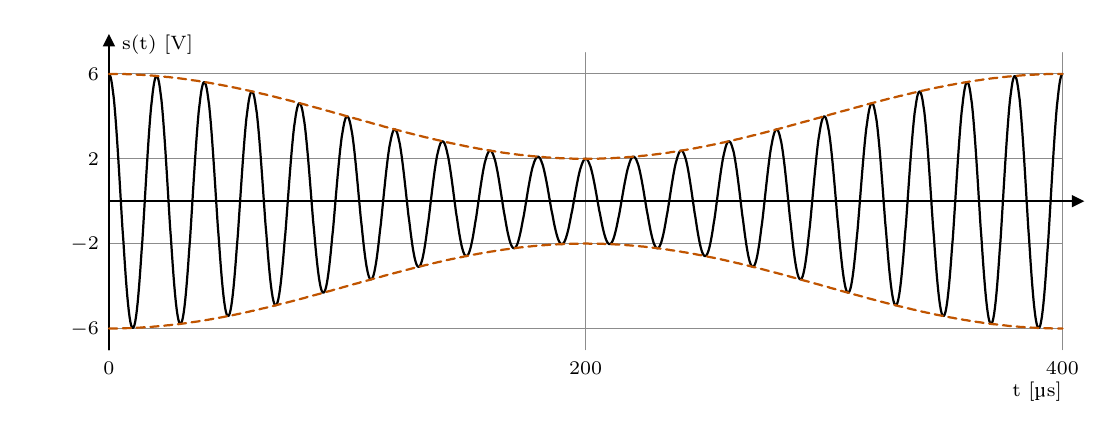
\begin{tikzpicture}[x=0.01985cm,y=-0.01985cm,line cap=round,line join=round]
\useasboundingbox (0,0) rectangle (680,240);
\path[draw=black!45,line width=0.35pt] (52,206) -- (52,16);
\path[draw=black!45,line width=0.35pt] (357,206) -- (357,16);
\path[draw=black!45,line width=0.35pt] (662,206) -- (662,16);
\path[draw=black!45,line width=0.35pt] (52,29.6) -- (662,29.6);
\path[draw=black!45,line width=0.35pt] (52,83.9) -- (662,83.9);
\path[draw=black!45,line width=0.35pt] (52,138.1) -- (662,138.1);
\path[draw=black!45,line width=0.35pt] (52,192.4) -- (662,192.4);
\path[draw=black,line width=0.7pt] (52,111) -- (670,111);
\path[fill=black,draw=none] (676,111) -- (668,107) -- (668,115) -- cycle;
\path[draw=black,line width=0.7pt] (52,206) -- (52,10);
\path[fill=black,draw=none] (52,4) -- (48,12) -- (56,12) -- cycle;
\node[anchor=base,inner sep=0pt,font=\scriptsize] at (52,222) {0};
\node[anchor=base,inner sep=0pt,font=\scriptsize] at (357,222) {200};
\node[anchor=base,inner sep=0pt,font=\scriptsize] at (662,222) {400};
\node[anchor=base east,inner sep=0pt,font=\scriptsize] at (46,33.6) {6};
\node[anchor=base east,inner sep=0pt,font=\scriptsize] at (46,87.9) {2};
\node[anchor=base east,inner sep=0pt,font=\scriptsize] at (46,142.1) {$-$2};
\node[anchor=base east,inner sep=0pt,font=\scriptsize] at (46,196.4) {$-$6};
\node[anchor=base east,inner sep=0pt,font=\scriptsize] at (662,236) {t [\textmu{}s]};
\node[anchor=base west,inner sep=0pt,font=\scriptsize] at (60,14) {s(t) [V]};
\path[draw=black,line width=0.8pt] (52,29.6) -- (52.5,30) -- (53,31.4) -- (53.5,33.6) -- (54,36.6) -- (54.5,40.5) -- (55.1,45.1) -- (55.6,50.5) -- (56.1,56.5) -- (56.6,63.2) -- (57.1,70.3) -- (57.6,77.9) -- (58.1,85.9) -- (58.6,94.1) -- (59.1,102.5) -- (59.6,111) -- (60.1,119.5) -- (60.6,127.9) -- (61.2,136.1) -- (61.7,144.1) -- (62.2,151.6) -- (62.7,158.8) -- (63.2,165.4) -- (63.7,171.4) -- (64.2,176.7) -- (64.7,181.3) -- (65.2,185.2) -- (65.7,188.2) -- (66.2,190.4) -- (66.7,191.7) -- (67.3,192.1) -- (67.8,191.6) -- (68.3,190.3) -- (68.8,188.1) -- (69.3,185) -- (69.8,181.1) -- (70.3,176.5) -- (70.8,171.1) -- (71.3,165.1) -- (71.8,158.5) -- (72.3,151.4) -- (72.8,143.9) -- (73.4,136) -- (73.9,127.8) -- (74.4,119.4) -- (74.9,111) -- (75.4,102.6) -- (75.9,94.2) -- (76.4,86.1) -- (76.9,78.2) -- (77.4,70.7) -- (77.9,63.7) -- (78.4,57.2) -- (78.9,51.3) -- (79.5,46) -- (80,41.4) -- (80.5,37.7) -- (81,34.7) -- (81.5,32.6) -- (82,31.3) -- (82.5,30.9) -- (83,31.4) -- (83.5,32.7) -- (84,34.9) -- (84.5,38) -- (85,41.8) -- (85.6,46.4) -- (86.1,51.7) -- (86.6,57.7) -- (87.1,64.2) -- (87.6,71.2) -- (88.1,78.6) -- (88.6,86.4) -- (89.1,94.5) -- (89.6,102.7) -- (90.1,111) -- (90.6,119.3) -- (91.1,127.5) -- (91.7,135.5) -- (92.2,143.2) -- (92.7,150.5) -- (93.2,157.4) -- (93.7,163.8) -- (94.2,169.6) -- (94.7,174.8) -- (95.2,179.2) -- (95.7,182.9) -- (96.2,185.8) -- (96.7,187.9) -- (97.2,189.1) -- (97.8,189.5) -- (98.3,189) -- (98.8,187.6) -- (99.3,185.4) -- (99.8,182.4) -- (100.3,178.7) -- (100.8,174.2) -- (101.3,169) -- (101.8,163.1) -- (102.3,156.8) -- (102.8,149.9) -- (103.3,142.6) -- (103.9,135) -- (104.4,127.1) -- (104.9,119.1) -- (105.4,111) -- (105.9,102.9) -- (106.4,94.9) -- (106.9,87.1) -- (107.4,79.6) -- (107.9,72.5) -- (108.4,65.8) -- (108.9,59.5) -- (109.4,53.9) -- (110,48.9) -- (110.5,44.6) -- (111,41) -- (111.5,38.3) -- (112,36.3) -- (112.5,35.1) -- (113,34.8) -- (113.5,35.3) -- (114,36.6) -- (114.5,38.7) -- (115,41.7) -- (115.5,45.3) -- (116.1,49.7) -- (116.6,54.8) -- (117.1,60.4) -- (117.6,66.6) -- (118.1,73.3) -- (118.6,80.4) -- (119.1,87.8) -- (119.6,95.4) -- (120.1,103.2) -- (120.6,111) -- (121.1,118.8) -- (121.6,126.5) -- (122.2,134.1) -- (122.7,141.3) -- (123.2,148.2) -- (123.7,154.7) -- (124.2,160.7) -- (124.7,166.1) -- (125.2,170.9) -- (125.7,175.1) -- (126.2,178.5) -- (126.7,181.2) -- (127.2,183.1) -- (127.7,184.2) -- (128.3,184.5) -- (128.8,184) -- (129.3,182.7) -- (129.8,180.6) -- (130.3,177.8) -- (130.8,174.2) -- (131.3,170) -- (131.8,165.1) -- (132.3,159.6) -- (132.8,153.6) -- (133.3,147.2) -- (133.8,140.4) -- (134.4,133.3) -- (134.9,126) -- (135.4,118.5) -- (135.9,111) -- (136.4,103.5) -- (136.9,96.1) -- (137.4,88.9) -- (137.9,81.9) -- (138.4,75.3) -- (138.9,69.1) -- (139.4,63.4) -- (139.9,58.2) -- (140.5,53.6) -- (141,49.7) -- (141.5,46.4) -- (142,43.9) -- (142.5,42.1) -- (143,41) -- (143.5,40.8) -- (144,41.3) -- (144.5,42.5) -- (145,44.5) -- (145.5,47.3) -- (146,50.7) -- (146.6,54.7) -- (147.1,59.4) -- (147.6,64.6) -- (148.1,70.3) -- (148.6,76.5) -- (149.1,83) -- (149.6,89.7) -- (150.1,96.7) -- (150.6,103.8) -- (151.1,111) -- (151.6,118.1) -- (152.1,125.2) -- (152.7,132) -- (153.2,138.6) -- (153.7,144.9) -- (154.2,150.8) -- (154.7,156.2) -- (155.2,161.2) -- (155.7,165.5) -- (156.2,169.2) -- (156.7,172.3) -- (157.2,174.7) -- (157.7,176.4) -- (158.2,177.4) -- (158.8,177.6) -- (159.3,177.1) -- (159.8,175.9) -- (160.3,174) -- (160.8,171.4) -- (161.3,168.1) -- (161.8,164.3) -- (162.3,159.8) -- (162.8,154.9) -- (163.3,149.5) -- (163.8,143.7) -- (164.3,137.5) -- (164.9,131.1) -- (165.4,124.5) -- (165.9,117.8) -- (166.4,111) -- (166.9,104.3) -- (167.4,97.6) -- (167.9,91.1) -- (168.4,84.9) -- (168.9,79) -- (169.4,73.5) -- (169.9,68.3) -- (170.4,63.7) -- (171,59.6) -- (171.5,56.1) -- (172,53.3) -- (172.5,51) -- (173,49.4) -- (173.5,48.5) -- (174,48.3) -- (174.5,48.8) -- (175,50) -- (175.5,51.8) -- (176,54.2) -- (176.5,57.3) -- (177.1,61) -- (177.6,65.1) -- (178.1,69.8) -- (178.6,74.9) -- (179.1,80.3) -- (179.6,86.1) -- (180.1,92.1) -- (180.6,98.3) -- (181.1,104.6) -- (181.6,111) -- (182.1,117.3) -- (182.6,123.5) -- (183.2,129.6) -- (183.7,135.4) -- (184.2,141) -- (184.7,146.1) -- (185.2,150.9) -- (185.7,155.2) -- (186.2,159) -- (186.7,162.3) -- (187.2,165) -- (187.7,167.1) -- (188.2,168.5) -- (188.7,169.4) -- (189.3,169.5) -- (189.8,169.1) -- (190.3,168) -- (190.8,166.3) -- (191.3,164) -- (191.8,161.1) -- (192.3,157.7) -- (192.8,153.8) -- (193.3,149.4) -- (193.8,144.7) -- (194.3,139.6) -- (194.8,134.2) -- (195.4,128.6) -- (195.9,122.8) -- (196.4,116.9) -- (196.9,111) -- (197.4,105.1) -- (197.9,99.3) -- (198.4,93.7) -- (198.9,88.3) -- (199.4,83.1) -- (199.9,78.3) -- (200.4,73.9) -- (200.9,69.9) -- (201.5,66.4) -- (202,63.4) -- (202.5,60.9) -- (203,59) -- (203.5,57.6) -- (204,56.9) -- (204.5,56.7) -- (205,57.2) -- (205.5,58.2) -- (206,59.8) -- (206.5,61.9) -- (207,64.6) -- (207.6,67.8) -- (208.1,71.4) -- (208.6,75.4) -- (209.1,79.8) -- (209.6,84.6) -- (210.1,89.6) -- (210.6,94.8) -- (211.1,100.1) -- (211.6,105.5) -- (212.1,111) -- (212.6,116.4) -- (213.1,121.8) -- (213.7,127) -- (214.2,132) -- (214.7,136.7) -- (215.2,141.2) -- (215.7,145.2) -- (216.2,148.9) -- (216.7,152.2) -- (217.2,154.9) -- (217.7,157.2) -- (218.2,159) -- (218.7,160.2) -- (219.2,160.9) -- (219.8,161) -- (220.3,160.6) -- (220.8,159.7) -- (221.3,158.2) -- (221.8,156.2) -- (222.3,153.7) -- (222.8,150.8) -- (223.3,147.5) -- (223.8,143.7) -- (224.3,139.7) -- (224.8,135.3) -- (225.3,130.7) -- (225.9,125.9) -- (226.4,121) -- (226.9,116) -- (227.4,111) -- (227.9,106) -- (228.4,101.1) -- (228.9,96.3) -- (229.4,91.7) -- (229.9,87.4) -- (230.4,83.3) -- (230.9,79.6) -- (231.4,76.2) -- (232,73.2) -- (232.5,70.7) -- (233,68.6) -- (233.5,67) -- (234,65.8) -- (234.5,65.2) -- (235,65.1) -- (235.5,65.5) -- (236,66.4) -- (236.5,67.7) -- (237,69.6) -- (237.5,71.8) -- (238.1,74.5) -- (238.6,77.6) -- (239.1,81) -- (239.6,84.7) -- (240.1,88.7) -- (240.6,92.9) -- (241.1,97.3) -- (241.6,101.8) -- (242.1,106.4) -- (242.6,111) -- (243.1,115.6) -- (243.6,120.1) -- (244.2,124.4) -- (244.7,128.6) -- (245.2,132.6) -- (245.7,136.3) -- (246.2,139.8) -- (246.7,142.8) -- (247.2,145.6) -- (247.7,147.9) -- (248.2,149.8) -- (248.7,151.3) -- (249.2,152.3) -- (249.7,152.9) -- (250.3,153) -- (250.8,152.6) -- (251.3,151.8) -- (251.8,150.5) -- (252.3,148.9) -- (252.8,146.8) -- (253.3,144.3) -- (253.8,141.5) -- (254.3,138.4) -- (254.8,135) -- (255.3,131.4) -- (255.8,127.5) -- (256.4,123.5) -- (256.9,119.4) -- (257.4,115.2) -- (257.9,111) -- (258.4,106.8) -- (258.9,102.7) -- (259.4,98.7) -- (259.9,94.9) -- (260.4,91.2) -- (260.9,87.9) -- (261.4,84.7) -- (261.9,81.9) -- (262.5,79.4) -- (263,77.3) -- (263.5,75.6) -- (264,74.2) -- (264.5,73.3) -- (265,72.8) -- (265.5,72.7) -- (266,73) -- (266.5,73.7) -- (267,74.9) -- (267.5,76.4) -- (268,78.3) -- (268.5,80.5) -- (269.1,83.1) -- (269.6,86) -- (270.1,89.1) -- (270.6,92.4) -- (271.1,95.9) -- (271.6,99.6) -- (272.1,103.3) -- (272.6,107.2) -- (273.1,111) -- (273.6,114.8) -- (274.1,118.6) -- (274.7,122.2) -- (275.2,125.7) -- (275.7,129.1) -- (276.2,132.2) -- (276.7,135) -- (277.2,137.6) -- (277.7,139.9) -- (278.2,141.8) -- (278.7,143.4) -- (279.2,144.7) -- (279.7,145.5) -- (280.2,146) -- (280.8,146.1) -- (281.3,145.8) -- (281.8,145.1) -- (282.3,144.1) -- (282.8,142.7) -- (283.3,141) -- (283.8,138.9) -- (284.3,136.6) -- (284.8,134) -- (285.3,131.1) -- (285.8,128.1) -- (286.3,124.8) -- (286.9,121.5) -- (287.4,118) -- (287.9,114.5) -- (288.4,111) -- (288.9,107.5) -- (289.4,104) -- (289.9,100.7) -- (290.4,97.5) -- (290.9,94.4) -- (291.4,91.5) -- (291.9,88.9) -- (292.4,86.5) -- (293,84.4) -- (293.5,82.6) -- (294,81.2) -- (294.5,80) -- (295,79.2) -- (295.5,78.8) -- (296,78.7) -- (296.5,78.9) -- (297,79.5) -- (297.5,80.5) -- (298,81.8) -- (298.5,83.4) -- (299.1,85.2) -- (299.6,87.4) -- (300.1,89.8) -- (300.6,92.4) -- (301.1,95.2) -- (301.6,98.2) -- (302.1,101.3) -- (302.6,104.5) -- (303.1,107.7) -- (303.6,111) -- (304.1,114.2) -- (304.6,117.4) -- (305.2,120.6) -- (305.7,123.5) -- (306.2,126.4) -- (306.7,129.1) -- (307.2,131.5) -- (307.7,133.7) -- (308.2,135.7) -- (308.7,137.4) -- (309.2,138.7) -- (309.7,139.8) -- (310.2,140.6) -- (310.7,141) -- (311.3,141.1) -- (311.8,140.9) -- (312.3,140.3) -- (312.8,139.4) -- (313.3,138.3) -- (313.8,136.8) -- (314.3,135) -- (314.8,133) -- (315.3,130.8) -- (315.8,128.4) -- (316.3,125.7) -- (316.8,123) -- (317.4,120.1) -- (317.9,117.1) -- (318.4,114.1) -- (318.9,111) -- (319.4,108) -- (319.9,104.9) -- (320.4,102) -- (320.9,99.2) -- (321.4,96.5) -- (321.9,94) -- (322.4,91.7) -- (322.9,89.6) -- (323.5,87.7) -- (324,86.1) -- (324.5,84.8) -- (325,83.8) -- (325.5,83.1) -- (326,82.6) -- (326.5,82.5) -- (327,82.7) -- (327.5,83.2) -- (328,84) -- (328.5,85.1) -- (329,86.5) -- (329.6,88.2) -- (330.1,90.1) -- (330.6,92.2) -- (331.1,94.5) -- (331.6,97) -- (332.1,99.6) -- (332.6,102.3) -- (333.1,105.2) -- (333.6,108.1) -- (334.1,111) -- (334.6,113.9) -- (335.1,116.8) -- (335.7,119.6) -- (336.2,122.3) -- (336.7,124.9) -- (337.2,127.3) -- (337.7,129.5) -- (338.2,131.5) -- (338.7,133.3) -- (339.2,134.9) -- (339.7,136.2) -- (340.2,137.2) -- (340.7,137.9) -- (341.2,138.3) -- (341.8,138.5) -- (342.3,138.3) -- (342.8,137.8) -- (343.3,137.1) -- (343.8,136) -- (344.3,134.7) -- (344.8,133.1) -- (345.3,131.3) -- (345.8,129.3) -- (346.3,127.1) -- (346.8,124.6) -- (347.3,122.1) -- (347.8,119.4) -- (348.4,116.7) -- (348.9,113.8) -- (349.4,111) -- (349.9,108.2) -- (350.4,105.3) -- (350.9,102.6) -- (351.4,99.9) -- (351.9,97.4) -- (352.4,95) -- (352.9,92.8) -- (353.4,90.8) -- (354,89) -- (354.5,87.5) -- (355,86.2) -- (355.5,85.2) -- (356,84.4) -- (356.5,84) -- (357,83.9) -- (357.5,84) -- (358,84.4) -- (358.5,85.2) -- (359,86.2) -- (359.5,87.5) -- (360.1,89) -- (360.6,90.8) -- (361.1,92.8) -- (361.6,95) -- (362.1,97.4) -- (362.6,99.9) -- (363.1,102.6) -- (363.6,105.3) -- (364.1,108.2) -- (364.6,111) -- (365.1,113.8) -- (365.6,116.7) -- (366.2,119.4) -- (366.7,122.1) -- (367.2,124.6) -- (367.7,127.1) -- (368.2,129.3) -- (368.7,131.3) -- (369.2,133.1) -- (369.7,134.7) -- (370.2,136) -- (370.7,137.1) -- (371.2,137.8) -- (371.7,138.3) -- (372.3,138.5) -- (372.8,138.3) -- (373.3,137.9) -- (373.8,137.2) -- (374.3,136.2) -- (374.8,134.9) -- (375.3,133.3) -- (375.8,131.5) -- (376.3,129.5) -- (376.8,127.3) -- (377.3,124.9) -- (377.8,122.3) -- (378.4,119.6) -- (378.9,116.8) -- (379.4,113.9) -- (379.9,111) -- (380.4,108.1) -- (380.9,105.2) -- (381.4,102.3) -- (381.9,99.6) -- (382.4,97) -- (382.9,94.5) -- (383.4,92.2) -- (383.9,90.1) -- (384.5,88.2) -- (385,86.5) -- (385.5,85.1) -- (386,84) -- (386.5,83.2) -- (387,82.7) -- (387.5,82.5) -- (388,82.6) -- (388.5,83.1) -- (389,83.8) -- (389.5,84.8) -- (390,86.1) -- (390.6,87.7) -- (391.1,89.6) -- (391.6,91.7) -- (392.1,94) -- (392.6,96.5) -- (393.1,99.2) -- (393.6,102) -- (394.1,104.9) -- (394.6,108) -- (395.1,111) -- (395.6,114.1) -- (396.1,117.1) -- (396.7,120.1) -- (397.2,123) -- (397.7,125.7) -- (398.2,128.4) -- (398.7,130.8) -- (399.2,133) -- (399.7,135) -- (400.2,136.8) -- (400.7,138.3) -- (401.2,139.4) -- (401.7,140.3) -- (402.2,140.9) -- (402.8,141.1) -- (403.3,141) -- (403.8,140.6) -- (404.3,139.8) -- (404.8,138.7) -- (405.3,137.4) -- (405.8,135.7) -- (406.3,133.7) -- (406.8,131.5) -- (407.3,129.1) -- (407.8,126.4) -- (408.3,123.5) -- (408.8,120.6) -- (409.4,117.4) -- (409.9,114.2) -- (410.4,111) -- (410.9,107.7) -- (411.4,104.5) -- (411.9,101.3) -- (412.4,98.2) -- (412.9,95.2) -- (413.4,92.4) -- (413.9,89.8) -- (414.4,87.4) -- (415,85.2) -- (415.5,83.4) -- (416,81.8) -- (416.5,80.5) -- (417,79.5) -- (417.5,78.9) -- (418,78.7) -- (418.5,78.8) -- (419,79.2) -- (419.5,80) -- (420,81.2) -- (420.5,82.6) -- (421.1,84.4) -- (421.6,86.5) -- (422.1,88.9) -- (422.6,91.5) -- (423.1,94.4) -- (423.6,97.5) -- (424.1,100.7) -- (424.6,104) -- (425.1,107.5) -- (425.6,111) -- (426.1,114.5) -- (426.6,118) -- (427.2,121.5) -- (427.7,124.8) -- (428.2,128.1) -- (428.7,131.1) -- (429.2,134) -- (429.7,136.6) -- (430.2,138.9) -- (430.7,141) -- (431.2,142.7) -- (431.7,144.1) -- (432.2,145.1) -- (432.7,145.8) -- (433.3,146.1) -- (433.8,146) -- (434.3,145.5) -- (434.8,144.7) -- (435.3,143.4) -- (435.8,141.8) -- (436.3,139.9) -- (436.8,137.6) -- (437.3,135) -- (437.8,132.2) -- (438.3,129.1) -- (438.8,125.7) -- (439.4,122.2) -- (439.9,118.6) -- (440.4,114.8) -- (440.9,111) -- (441.4,107.2) -- (441.9,103.3) -- (442.4,99.6) -- (442.9,95.9) -- (443.4,92.4) -- (443.9,89.1) -- (444.4,86) -- (444.9,83.1) -- (445.5,80.5) -- (446,78.3) -- (446.5,76.4) -- (447,74.9) -- (447.5,73.7) -- (448,73) -- (448.5,72.7) -- (449,72.8) -- (449.5,73.3) -- (450,74.2) -- (450.5,75.6) -- (451,77.3) -- (451.6,79.4) -- (452.1,81.9) -- (452.6,84.7) -- (453.1,87.9) -- (453.6,91.2) -- (454.1,94.9) -- (454.6,98.7) -- (455.1,102.7) -- (455.6,106.8) -- (456.1,111) -- (456.6,115.2) -- (457.1,119.4) -- (457.7,123.5) -- (458.2,127.5) -- (458.7,131.4) -- (459.2,135) -- (459.7,138.4) -- (460.2,141.5) -- (460.7,144.3) -- (461.2,146.8) -- (461.7,148.9) -- (462.2,150.5) -- (462.7,151.8) -- (463.2,152.6) -- (463.8,153) -- (464.3,152.9) -- (464.8,152.3) -- (465.3,151.3) -- (465.8,149.8) -- (466.3,147.9) -- (466.8,145.6) -- (467.3,142.8) -- (467.8,139.8) -- (468.3,136.3) -- (468.8,132.6) -- (469.3,128.6) -- (469.9,124.4) -- (470.4,120.1) -- (470.9,115.6) -- (471.4,111) -- (471.9,106.4) -- (472.4,101.8) -- (472.9,97.3) -- (473.4,92.9) -- (473.9,88.7) -- (474.4,84.7) -- (474.9,81) -- (475.4,77.6) -- (476,74.5) -- (476.5,71.8) -- (477,69.6) -- (477.5,67.7) -- (478,66.4) -- (478.5,65.5) -- (479,65.1) -- (479.5,65.2) -- (480,65.8) -- (480.5,67) -- (481,68.6) -- (481.5,70.7) -- (482.1,73.2) -- (482.6,76.2) -- (483.1,79.6) -- (483.6,83.3) -- (484.1,87.4) -- (484.6,91.7) -- (485.1,96.3) -- (485.6,101.1) -- (486.1,106) -- (486.6,111) -- (487.1,116) -- (487.6,121) -- (488.2,125.9) -- (488.7,130.7) -- (489.2,135.3) -- (489.7,139.7) -- (490.2,143.7) -- (490.7,147.5) -- (491.2,150.8) -- (491.7,153.7) -- (492.2,156.2) -- (492.7,158.2) -- (493.2,159.7) -- (493.7,160.6) -- (494.3,161) -- (494.8,160.9) -- (495.3,160.2) -- (495.8,159) -- (496.3,157.2) -- (496.8,154.9) -- (497.3,152.2) -- (497.8,148.9) -- (498.3,145.2) -- (498.8,141.2) -- (499.3,136.7) -- (499.8,132) -- (500.4,127) -- (500.9,121.8) -- (501.4,116.4) -- (501.9,111) -- (502.4,105.5) -- (502.9,100.1) -- (503.4,94.8) -- (503.9,89.6) -- (504.4,84.6) -- (504.9,79.8) -- (505.4,75.4) -- (505.9,71.4) -- (506.5,67.8) -- (507,64.6) -- (507.5,61.9) -- (508,59.8) -- (508.5,58.2) -- (509,57.2) -- (509.5,56.7) -- (510,56.9) -- (510.5,57.6) -- (511,59) -- (511.5,60.9) -- (512,63.4) -- (512.6,66.4) -- (513.1,69.9) -- (513.6,73.9) -- (514.1,78.3) -- (514.6,83.1) -- (515.1,88.3) -- (515.6,93.7) -- (516.1,99.3) -- (516.6,105.1) -- (517.1,111) -- (517.6,116.9) -- (518.1,122.8) -- (518.7,128.6) -- (519.2,134.2) -- (519.7,139.6) -- (520.2,144.7) -- (520.7,149.4) -- (521.2,153.8) -- (521.7,157.7) -- (522.2,161.1) -- (522.7,164) -- (523.2,166.3) -- (523.7,168) -- (524.2,169.1) -- (524.8,169.5) -- (525.3,169.4) -- (525.8,168.5) -- (526.3,167.1) -- (526.8,165) -- (527.3,162.3) -- (527.8,159) -- (528.3,155.2) -- (528.8,150.9) -- (529.3,146.1) -- (529.8,141) -- (530.3,135.4) -- (530.9,129.6) -- (531.4,123.5) -- (531.9,117.3) -- (532.4,111) -- (532.9,104.6) -- (533.4,98.3) -- (533.9,92.1) -- (534.4,86.1) -- (534.9,80.3) -- (535.4,74.9) -- (535.9,69.8) -- (536.4,65.1) -- (537,61) -- (537.5,57.3) -- (538,54.2) -- (538.5,51.8) -- (539,50) -- (539.5,48.8) -- (540,48.3) -- (540.5,48.5) -- (541,49.4) -- (541.5,51) -- (542,53.3) -- (542.5,56.1) -- (543.1,59.6) -- (543.6,63.7) -- (544.1,68.3) -- (544.6,73.5) -- (545.1,79) -- (545.6,84.9) -- (546.1,91.1) -- (546.6,97.6) -- (547.1,104.3) -- (547.6,111) -- (548.1,117.8) -- (548.6,124.5) -- (549.2,131.1) -- (549.7,137.5) -- (550.2,143.7) -- (550.7,149.5) -- (551.2,154.9) -- (551.7,159.8) -- (552.2,164.3) -- (552.7,168.1) -- (553.2,171.4) -- (553.7,174) -- (554.2,175.9) -- (554.7,177.1) -- (555.3,177.6) -- (555.8,177.4) -- (556.3,176.4) -- (556.8,174.7) -- (557.3,172.3) -- (557.8,169.2) -- (558.3,165.5) -- (558.8,161.2) -- (559.3,156.2) -- (559.8,150.8) -- (560.3,144.9) -- (560.8,138.6) -- (561.3,132) -- (561.9,125.2) -- (562.4,118.1) -- (562.9,111) -- (563.4,103.8) -- (563.9,96.7) -- (564.4,89.7) -- (564.9,83) -- (565.4,76.5) -- (565.9,70.3) -- (566.4,64.6) -- (566.9,59.4) -- (567.4,54.7) -- (568,50.7) -- (568.5,47.3) -- (569,44.5) -- (569.5,42.5) -- (570,41.3) -- (570.5,40.8) -- (571,41) -- (571.5,42.1) -- (572,43.9) -- (572.5,46.4) -- (573,49.7) -- (573.6,53.6) -- (574.1,58.2) -- (574.6,63.4) -- (575.1,69.1) -- (575.6,75.3) -- (576.1,81.9) -- (576.6,88.9) -- (577.1,96.1) -- (577.6,103.5) -- (578.1,111) -- (578.6,118.5) -- (579.1,126) -- (579.7,133.3) -- (580.2,140.4) -- (580.7,147.2) -- (581.2,153.6) -- (581.7,159.6) -- (582.2,165.1) -- (582.7,170) -- (583.2,174.2) -- (583.7,177.8) -- (584.2,180.6) -- (584.7,182.7) -- (585.2,184) -- (585.8,184.5) -- (586.3,184.2) -- (586.8,183.1) -- (587.3,181.2) -- (587.8,178.5) -- (588.3,175.1) -- (588.8,170.9) -- (589.3,166.1) -- (589.8,160.7) -- (590.3,154.7) -- (590.8,148.2) -- (591.3,141.3) -- (591.9,134.1) -- (592.4,126.5) -- (592.9,118.8) -- (593.4,111) -- (593.9,103.2) -- (594.4,95.4) -- (594.9,87.8) -- (595.4,80.4) -- (595.9,73.3) -- (596.4,66.6) -- (596.9,60.4) -- (597.4,54.8) -- (598,49.7) -- (598.5,45.3) -- (599,41.7) -- (599.5,38.7) -- (600,36.6) -- (600.5,35.3) -- (601,34.8) -- (601.5,35.1) -- (602,36.3) -- (602.5,38.3) -- (603,41) -- (603.5,44.6) -- (604.1,48.9) -- (604.6,53.9) -- (605.1,59.5) -- (605.6,65.8) -- (606.1,72.5) -- (606.6,79.6) -- (607.1,87.1) -- (607.6,94.9) -- (608.1,102.9) -- (608.6,111) -- (609.1,119.1) -- (609.6,127.1) -- (610.2,135) -- (610.7,142.6) -- (611.2,149.9) -- (611.7,156.8) -- (612.2,163.1) -- (612.7,169) -- (613.2,174.2) -- (613.7,178.7) -- (614.2,182.4) -- (614.7,185.4) -- (615.2,187.6) -- (615.7,189) -- (616.3,189.5) -- (616.8,189.1) -- (617.3,187.9) -- (617.8,185.8) -- (618.3,182.9) -- (618.8,179.2) -- (619.3,174.8) -- (619.8,169.6) -- (620.3,163.8) -- (620.8,157.4) -- (621.3,150.5) -- (621.8,143.2) -- (622.4,135.5) -- (622.9,127.5) -- (623.4,119.3) -- (623.9,111) -- (624.4,102.7) -- (624.9,94.5) -- (625.4,86.4) -- (625.9,78.6) -- (626.4,71.2) -- (626.9,64.2) -- (627.4,57.7) -- (627.9,51.7) -- (628.4,46.4) -- (629,41.8) -- (629.5,38) -- (630,34.9) -- (630.5,32.7) -- (631,31.4) -- (631.5,30.9) -- (632,31.3) -- (632.5,32.6) -- (633,34.7) -- (633.5,37.7) -- (634,41.4) -- (634.6,46) -- (635.1,51.3) -- (635.6,57.2) -- (636.1,63.7) -- (636.6,70.7) -- (637.1,78.2) -- (637.6,86.1) -- (638.1,94.2) -- (638.6,102.6) -- (639.1,111) -- (639.6,119.4) -- (640.1,127.8) -- (640.7,136) -- (641.2,143.9) -- (641.7,151.4) -- (642.2,158.5) -- (642.7,165.1) -- (643.2,171.1) -- (643.7,176.5) -- (644.2,181.1) -- (644.7,185) -- (645.2,188.1) -- (645.7,190.3) -- (646.2,191.6) -- (646.8,192.1) -- (647.3,191.7) -- (647.8,190.4) -- (648.3,188.2) -- (648.8,185.2) -- (649.3,181.3) -- (649.8,176.7) -- (650.3,171.4) -- (650.8,165.4) -- (651.3,158.8) -- (651.8,151.6) -- (652.3,144.1) -- (652.9,136.1) -- (653.4,127.9) -- (653.9,119.5) -- (654.4,111) -- (654.9,102.5) -- (655.4,94.1) -- (655.9,85.9) -- (656.4,77.9) -- (656.9,70.3) -- (657.4,63.2) -- (657.9,56.5) -- (658.4,50.5) -- (659,45.1) -- (659.5,40.5) -- (660,36.6) -- (660.5,33.6) -- (661,31.4) -- (661.5,30) -- (662,29.6);
\path[draw=cB,line width=0.8pt,dash pattern=on 3pt off 2pt] (52,29.6) -- (52.8,29.6) -- (53.5,29.6) -- (54.3,29.6) -- (55.1,29.6) -- (55.8,29.6) -- (56.6,29.6) -- (57.3,29.6) -- (58.1,29.6) -- (58.9,29.6) -- (59.6,29.7) -- (60.4,29.7) -- (61.2,29.7) -- (61.9,29.7) -- (62.7,29.7) -- (63.4,29.8) -- (64.2,29.8) -- (65,29.8) -- (65.7,29.8) -- (66.5,29.9) -- (67.3,29.9) -- (68,29.9) -- (68.8,30) -- (69.5,30) -- (70.3,30.1) -- (71.1,30.1) -- (71.8,30.1) -- (72.6,30.2) -- (73.4,30.2) -- (74.1,30.3) -- (74.9,30.3) -- (75.6,30.4) -- (76.4,30.4) -- (77.2,30.5) -- (77.9,30.5) -- (78.7,30.6) -- (79.5,30.6) -- (80.2,30.7) -- (81,30.8) -- (81.7,30.8) -- (82.5,30.9) -- (83.3,31) -- (84,31) -- (84.8,31.1) -- (85.6,31.2) -- (86.3,31.2) -- (87.1,31.3) -- (87.8,31.4) -- (88.6,31.5) -- (89.4,31.6) -- (90.1,31.6) -- (90.9,31.7) -- (91.7,31.8) -- (92.4,31.9) -- (93.2,32) -- (93.9,32.1) -- (94.7,32.2) -- (95.5,32.2) -- (96.2,32.3) -- (97,32.4) -- (97.8,32.5) -- (98.5,32.6) -- (99.3,32.7) -- (100,32.8) -- (100.8,32.9) -- (101.6,33) -- (102.3,33.1) -- (103.1,33.2) -- (103.9,33.4) -- (104.6,33.5) -- (105.4,33.6) -- (106.1,33.7) -- (106.9,33.8) -- (107.7,33.9) -- (108.4,34) -- (109.2,34.1) -- (110,34.3) -- (110.7,34.4) -- (111.5,34.5) -- (112.2,34.6) -- (113,34.8) -- (113.8,34.9) -- (114.5,35) -- (115.3,35.1) -- (116.1,35.3) -- (116.8,35.4) -- (117.6,35.5) -- (118.3,35.7) -- (119.1,35.8) -- (119.9,35.9) -- (120.6,36.1) -- (121.4,36.2) -- (122.2,36.4) -- (122.9,36.5) -- (123.7,36.6) -- (124.4,36.8) -- (125.2,36.9) -- (126,37.1) -- (126.7,37.2) -- (127.5,37.4) -- (128.3,37.5) -- (129,37.7) -- (129.8,37.8) -- (130.5,38) -- (131.3,38.1) -- (132.1,38.3) -- (132.8,38.4) -- (133.6,38.6) -- (134.4,38.8) -- (135.1,38.9) -- (135.9,39.1) -- (136.6,39.2) -- (137.4,39.4) -- (138.2,39.6) -- (138.9,39.7) -- (139.7,39.9) -- (140.5,40.1) -- (141.2,40.2) -- (142,40.4) -- (142.7,40.6) -- (143.5,40.8) -- (144.3,40.9) -- (145,41.1) -- (145.8,41.3) -- (146.6,41.5) -- (147.3,41.6) -- (148.1,41.8) -- (148.8,42) -- (149.6,42.2) -- (150.4,42.4) -- (151.1,42.5) -- (151.9,42.7) -- (152.7,42.9) -- (153.4,43.1) -- (154.2,43.3) -- (154.9,43.5) -- (155.7,43.6) -- (156.5,43.8) -- (157.2,44) -- (158,44.2) -- (158.8,44.4) -- (159.5,44.6) -- (160.3,44.8) -- (161,45) -- (161.8,45.2) -- (162.6,45.4) -- (163.3,45.5) -- (164.1,45.7) -- (164.9,45.9) -- (165.6,46.1) -- (166.4,46.3) -- (167.1,46.5) -- (167.9,46.7) -- (168.7,46.9) -- (169.4,47.1) -- (170.2,47.3) -- (171,47.5) -- (171.7,47.7) -- (172.5,47.9) -- (173.2,48.1) -- (174,48.3) -- (174.8,48.5) -- (175.5,48.7) -- (176.3,48.9) -- (177.1,49.1) -- (177.8,49.3) -- (178.6,49.6) -- (179.3,49.8) -- (180.1,50) -- (180.9,50.2) -- (181.6,50.4) -- (182.4,50.6) -- (183.2,50.8) -- (183.9,51) -- (184.7,51.2) -- (185.4,51.4) -- (186.2,51.6) -- (187,51.8) -- (187.7,52) -- (188.5,52.3) -- (189.3,52.5) -- (190,52.7) -- (190.8,52.9) -- (191.5,53.1) -- (192.3,53.3) -- (193.1,53.5) -- (193.8,53.7) -- (194.6,53.9) -- (195.4,54.2) -- (196.1,54.4) -- (196.9,54.6) -- (197.6,54.8) -- (198.4,55) -- (199.2,55.2) -- (199.9,55.4) -- (200.7,55.6) -- (201.5,55.9) -- (202.2,56.1) -- (203,56.3) -- (203.7,56.5) -- (204.5,56.7) -- (205.3,56.9) -- (206,57.1) -- (206.8,57.4) -- (207.6,57.6) -- (208.3,57.8) -- (209.1,58) -- (209.8,58.2) -- (210.6,58.4) -- (211.4,58.6) -- (212.1,58.8) -- (212.9,59.1) -- (213.7,59.3) -- (214.4,59.5) -- (215.2,59.7) -- (215.9,59.9) -- (216.7,60.1) -- (217.5,60.3) -- (218.2,60.5) -- (219,60.7) -- (219.8,61) -- (220.5,61.2) -- (221.3,61.4) -- (222,61.6) -- (222.8,61.8) -- (223.6,62) -- (224.3,62.2) -- (225.1,62.4) -- (225.9,62.6) -- (226.6,62.8) -- (227.4,63.1) -- (228.1,63.3) -- (228.9,63.5) -- (229.7,63.7) -- (230.4,63.9) -- (231.2,64.1) -- (232,64.3) -- (232.7,64.5) -- (233.5,64.7) -- (234.2,64.9) -- (235,65.1) -- (235.8,65.3) -- (236.5,65.5) -- (237.3,65.7) -- (238.1,65.9) -- (238.8,66.1) -- (239.6,66.3) -- (240.3,66.5) -- (241.1,66.7) -- (241.9,66.9) -- (242.6,67.1) -- (243.4,67.3) -- (244.2,67.5) -- (244.9,67.7) -- (245.7,67.9) -- (246.4,68.1) -- (247.2,68.3) -- (248,68.5) -- (248.7,68.7) -- (249.5,68.8) -- (250.3,69) -- (251,69.2) -- (251.8,69.4) -- (252.5,69.6) -- (253.3,69.8) -- (254.1,70) -- (254.8,70.2) -- (255.6,70.3) -- (256.4,70.5) -- (257.1,70.7) -- (257.9,70.9) -- (258.6,71.1) -- (259.4,71.3) -- (260.2,71.4) -- (260.9,71.6) -- (261.7,71.8) -- (262.5,72) -- (263.2,72.1) -- (264,72.3) -- (264.7,72.5) -- (265.5,72.7) -- (266.3,72.8) -- (267,73) -- (267.8,73.2) -- (268.5,73.4) -- (269.3,73.5) -- (270.1,73.7) -- (270.8,73.9) -- (271.6,74) -- (272.4,74.2) -- (273.1,74.3) -- (273.9,74.5) -- (274.7,74.7) -- (275.4,74.8) -- (276.2,75) -- (276.9,75.1) -- (277.7,75.3) -- (278.5,75.4) -- (279.2,75.6) -- (280,75.8) -- (280.8,75.9) -- (281.5,76.1) -- (282.3,76.2) -- (283,76.4) -- (283.8,76.5) -- (284.6,76.6) -- (285.3,76.8) -- (286.1,76.9) -- (286.9,77.1) -- (287.6,77.2) -- (288.4,77.4) -- (289.1,77.5) -- (289.9,77.6) -- (290.7,77.8) -- (291.4,77.9) -- (292.2,78) -- (293,78.2) -- (293.7,78.3) -- (294.5,78.4) -- (295.2,78.5) -- (296,78.7) -- (296.8,78.8) -- (297.5,78.9) -- (298.3,79) -- (299.1,79.2) -- (299.8,79.3) -- (300.6,79.4) -- (301.3,79.5) -- (302.1,79.6) -- (302.9,79.7) -- (303.6,79.9) -- (304.4,80) -- (305.2,80.1) -- (305.9,80.2) -- (306.7,80.3) -- (307.4,80.4) -- (308.2,80.5) -- (309,80.6) -- (309.7,80.7) -- (310.5,80.8) -- (311.3,80.9) -- (312,81) -- (312.8,81.1) -- (313.5,81.2) -- (314.3,81.3) -- (315.1,81.4) -- (315.8,81.5) -- (316.6,81.5) -- (317.4,81.6) -- (318.1,81.7) -- (318.9,81.8) -- (319.6,81.9) -- (320.4,82) -- (321.2,82) -- (321.9,82.1) -- (322.7,82.2) -- (323.5,82.3) -- (324.2,82.3) -- (325,82.4) -- (325.7,82.5) -- (326.5,82.5) -- (327.3,82.6) -- (328,82.7) -- (328.8,82.7) -- (329.6,82.8) -- (330.3,82.8) -- (331.1,82.9) -- (331.8,83) -- (332.6,83) -- (333.4,83.1) -- (334.1,83.1) -- (334.9,83.2) -- (335.7,83.2) -- (336.4,83.2) -- (337.2,83.3) -- (337.9,83.3) -- (338.7,83.4) -- (339.5,83.4) -- (340.2,83.5) -- (341,83.5) -- (341.8,83.5) -- (342.5,83.6) -- (343.3,83.6) -- (344,83.6) -- (344.8,83.6) -- (345.6,83.7) -- (346.3,83.7) -- (347.1,83.7) -- (347.8,83.7) -- (348.6,83.8) -- (349.4,83.8) -- (350.1,83.8) -- (350.9,83.8) -- (351.7,83.8) -- (352.4,83.8) -- (353.2,83.8) -- (354,83.8) -- (354.7,83.8) -- (355.5,83.9) -- (356.2,83.9) -- (357,83.9) -- (357.8,83.9) -- (358.5,83.9) -- (359.3,83.8) -- (360.1,83.8) -- (360.8,83.8) -- (361.6,83.8) -- (362.3,83.8) -- (363.1,83.8) -- (363.9,83.8) -- (364.6,83.8) -- (365.4,83.8) -- (366.2,83.7) -- (366.9,83.7) -- (367.7,83.7) -- (368.4,83.7) -- (369.2,83.6) -- (370,83.6) -- (370.7,83.6) -- (371.5,83.6) -- (372.3,83.5) -- (373,83.5) -- (373.8,83.5) -- (374.5,83.4) -- (375.3,83.4) -- (376.1,83.3) -- (376.8,83.3) -- (377.6,83.2) -- (378.4,83.2) -- (379.1,83.2) -- (379.9,83.1) -- (380.6,83.1) -- (381.4,83) -- (382.2,83) -- (382.9,82.9) -- (383.7,82.8) -- (384.5,82.8) -- (385.2,82.7) -- (386,82.7) -- (386.7,82.6) -- (387.5,82.5) -- (388.3,82.5) -- (389,82.4) -- (389.8,82.3) -- (390.6,82.3) -- (391.3,82.2) -- (392.1,82.1) -- (392.8,82) -- (393.6,82) -- (394.4,81.9) -- (395.1,81.8) -- (395.9,81.7) -- (396.7,81.6) -- (397.4,81.5) -- (398.2,81.5) -- (398.9,81.4) -- (399.7,81.3) -- (400.5,81.2) -- (401.2,81.1) -- (402,81) -- (402.8,80.9) -- (403.5,80.8) -- (404.3,80.7) -- (405,80.6) -- (405.8,80.5) -- (406.6,80.4) -- (407.3,80.3) -- (408.1,80.2) -- (408.8,80.1) -- (409.6,80) -- (410.4,79.9) -- (411.1,79.7) -- (411.9,79.6) -- (412.7,79.5) -- (413.4,79.4) -- (414.2,79.3) -- (415,79.2) -- (415.7,79) -- (416.5,78.9) -- (417.2,78.8) -- (418,78.7) -- (418.8,78.5) -- (419.5,78.4) -- (420.3,78.3) -- (421.1,78.2) -- (421.8,78) -- (422.6,77.9) -- (423.3,77.8) -- (424.1,77.6) -- (424.9,77.5) -- (425.6,77.4) -- (426.4,77.2) -- (427.2,77.1) -- (427.9,76.9) -- (428.7,76.8) -- (429.4,76.6) -- (430.2,76.5) -- (431,76.4) -- (431.7,76.2) -- (432.5,76.1) -- (433.3,75.9) -- (434,75.8) -- (434.8,75.6) -- (435.5,75.4) -- (436.3,75.3) -- (437.1,75.1) -- (437.8,75) -- (438.6,74.8) -- (439.4,74.7) -- (440.1,74.5) -- (440.9,74.3) -- (441.6,74.2) -- (442.4,74) -- (443.2,73.9) -- (443.9,73.7) -- (444.7,73.5) -- (445.5,73.4) -- (446.2,73.2) -- (447,73) -- (447.7,72.8) -- (448.5,72.7) -- (449.3,72.5) -- (450,72.3) -- (450.8,72.1) -- (451.6,72) -- (452.3,71.8) -- (453.1,71.6) -- (453.8,71.4) -- (454.6,71.3) -- (455.4,71.1) -- (456.1,70.9) -- (456.9,70.7) -- (457.7,70.5) -- (458.4,70.3) -- (459.2,70.2) -- (459.9,70) -- (460.7,69.8) -- (461.5,69.6) -- (462.2,69.4) -- (463,69.2) -- (463.8,69) -- (464.5,68.8) -- (465.3,68.7) -- (466,68.5) -- (466.8,68.3) -- (467.6,68.1) -- (468.3,67.9) -- (469.1,67.7) -- (469.9,67.5) -- (470.6,67.3) -- (471.4,67.1) -- (472.1,66.9) -- (472.9,66.7) -- (473.7,66.5) -- (474.4,66.3) -- (475.2,66.1) -- (476,65.9) -- (476.7,65.7) -- (477.5,65.5) -- (478.2,65.3) -- (479,65.1) -- (479.8,64.9) -- (480.5,64.7) -- (481.3,64.5) -- (482.1,64.3) -- (482.8,64.1) -- (483.6,63.9) -- (484.3,63.7) -- (485.1,63.5) -- (485.9,63.3) -- (486.6,63.1) -- (487.4,62.8) -- (488.2,62.6) -- (488.9,62.4) -- (489.7,62.2) -- (490.4,62) -- (491.2,61.8) -- (492,61.6) -- (492.7,61.4) -- (493.5,61.2) -- (494.3,61) -- (495,60.7) -- (495.8,60.5) -- (496.5,60.3) -- (497.3,60.1) -- (498.1,59.9) -- (498.8,59.7) -- (499.6,59.5) -- (500.4,59.3) -- (501.1,59.1) -- (501.9,58.8) -- (502.6,58.6) -- (503.4,58.4) -- (504.2,58.2) -- (504.9,58) -- (505.7,57.8) -- (506.5,57.6) -- (507.2,57.4) -- (508,57.1) -- (508.7,56.9) -- (509.5,56.7) -- (510.3,56.5) -- (511,56.3) -- (511.8,56.1) -- (512.6,55.9) -- (513.3,55.6) -- (514.1,55.4) -- (514.8,55.2) -- (515.6,55) -- (516.4,54.8) -- (517.1,54.6) -- (517.9,54.4) -- (518.7,54.2) -- (519.4,53.9) -- (520.2,53.7) -- (520.9,53.5) -- (521.7,53.3) -- (522.5,53.1) -- (523.2,52.9) -- (524,52.7) -- (524.8,52.5) -- (525.5,52.3) -- (526.3,52) -- (527,51.8) -- (527.8,51.6) -- (528.6,51.4) -- (529.3,51.2) -- (530.1,51) -- (530.9,50.8) -- (531.6,50.6) -- (532.4,50.4) -- (533.1,50.2) -- (533.9,50) -- (534.7,49.8) -- (535.4,49.6) -- (536.2,49.3) -- (537,49.1) -- (537.7,48.9) -- (538.5,48.7) -- (539.2,48.5) -- (540,48.3) -- (540.8,48.1) -- (541.5,47.9) -- (542.3,47.7) -- (543.1,47.5) -- (543.8,47.3) -- (544.6,47.1) -- (545.3,46.9) -- (546.1,46.7) -- (546.9,46.5) -- (547.6,46.3) -- (548.4,46.1) -- (549.2,45.9) -- (549.9,45.7) -- (550.7,45.5) -- (551.4,45.4) -- (552.2,45.2) -- (553,45) -- (553.7,44.8) -- (554.5,44.6) -- (555.3,44.4) -- (556,44.2) -- (556.8,44) -- (557.5,43.8) -- (558.3,43.6) -- (559.1,43.5) -- (559.8,43.3) -- (560.6,43.1) -- (561.3,42.9) -- (562.1,42.7) -- (562.9,42.5) -- (563.6,42.4) -- (564.4,42.2) -- (565.2,42) -- (565.9,41.8) -- (566.7,41.6) -- (567.4,41.5) -- (568.2,41.3) -- (569,41.1) -- (569.7,40.9) -- (570.5,40.8) -- (571.3,40.6) -- (572,40.4) -- (572.8,40.2) -- (573.6,40.1) -- (574.3,39.9) -- (575.1,39.7) -- (575.8,39.6) -- (576.6,39.4) -- (577.4,39.2) -- (578.1,39.1) -- (578.9,38.9) -- (579.7,38.8) -- (580.4,38.6) -- (581.2,38.4) -- (581.9,38.3) -- (582.7,38.1) -- (583.5,38) -- (584.2,37.8) -- (585,37.7) -- (585.8,37.5) -- (586.5,37.4) -- (587.3,37.2) -- (588,37.1) -- (588.8,36.9) -- (589.6,36.8) -- (590.3,36.6) -- (591.1,36.5) -- (591.9,36.4) -- (592.6,36.2) -- (593.4,36.1) -- (594.1,35.9) -- (594.9,35.8) -- (595.7,35.7) -- (596.4,35.5) -- (597.2,35.4) -- (598,35.3) -- (598.7,35.1) -- (599.5,35) -- (600.2,34.9) -- (601,34.8) -- (601.8,34.6) -- (602.5,34.5) -- (603.3,34.4) -- (604.1,34.3) -- (604.8,34.1) -- (605.6,34) -- (606.3,33.9) -- (607.1,33.8) -- (607.9,33.7) -- (608.6,33.6) -- (609.4,33.5) -- (610.2,33.4) -- (610.9,33.2) -- (611.7,33.1) -- (612.4,33) -- (613.2,32.9) -- (614,32.8) -- (614.7,32.7) -- (615.5,32.6) -- (616.3,32.5) -- (617,32.4) -- (617.8,32.3) -- (618.5,32.2) -- (619.3,32.2) -- (620.1,32.1) -- (620.8,32) -- (621.6,31.9) -- (622.4,31.8) -- (623.1,31.7) -- (623.9,31.6) -- (624.6,31.6) -- (625.4,31.5) -- (626.2,31.4) -- (626.9,31.3) -- (627.7,31.2) -- (628.4,31.2) -- (629.2,31.1) -- (630,31) -- (630.7,31) -- (631.5,30.9) -- (632.3,30.8) -- (633,30.8) -- (633.8,30.7) -- (634.6,30.6) -- (635.3,30.6) -- (636.1,30.5) -- (636.8,30.5) -- (637.6,30.4) -- (638.4,30.4) -- (639.1,30.3) -- (639.9,30.3) -- (640.7,30.2) -- (641.4,30.2) -- (642.2,30.1) -- (642.9,30.1) -- (643.7,30.1) -- (644.5,30) -- (645.2,30) -- (646,29.9) -- (646.8,29.9) -- (647.5,29.9) -- (648.3,29.8) -- (649,29.8) -- (649.8,29.8) -- (650.6,29.8) -- (651.3,29.7) -- (652.1,29.7) -- (652.9,29.7) -- (653.6,29.7) -- (654.4,29.7) -- (655.1,29.6) -- (655.9,29.6) -- (656.7,29.6) -- (657.4,29.6) -- (658.2,29.6) -- (659,29.6) -- (659.7,29.6) -- (660.5,29.6) -- (661.2,29.6) -- (662,29.6);
\path[draw=cB,line width=0.8pt,dash pattern=on 3pt off 2pt] (52,192.4) -- (52.8,192.4) -- (53.5,192.4) -- (54.3,192.4) -- (55.1,192.4) -- (55.8,192.4) -- (56.6,192.4) -- (57.3,192.4) -- (58.1,192.4) -- (58.9,192.4) -- (59.6,192.3) -- (60.4,192.3) -- (61.2,192.3) -- (61.9,192.3) -- (62.7,192.3) -- (63.4,192.2) -- (64.2,192.2) -- (65,192.2) -- (65.7,192.2) -- (66.5,192.1) -- (67.3,192.1) -- (68,192.1) -- (68.8,192) -- (69.5,192) -- (70.3,191.9) -- (71.1,191.9) -- (71.8,191.9) -- (72.6,191.8) -- (73.4,191.8) -- (74.1,191.7) -- (74.9,191.7) -- (75.6,191.6) -- (76.4,191.6) -- (77.2,191.5) -- (77.9,191.5) -- (78.7,191.4) -- (79.5,191.4) -- (80.2,191.3) -- (81,191.2) -- (81.7,191.2) -- (82.5,191.1) -- (83.3,191) -- (84,191) -- (84.8,190.9) -- (85.6,190.8) -- (86.3,190.8) -- (87.1,190.7) -- (87.8,190.6) -- (88.6,190.5) -- (89.4,190.4) -- (90.1,190.4) -- (90.9,190.3) -- (91.7,190.2) -- (92.4,190.1) -- (93.2,190) -- (93.9,189.9) -- (94.7,189.8) -- (95.5,189.8) -- (96.2,189.7) -- (97,189.6) -- (97.8,189.5) -- (98.5,189.4) -- (99.3,189.3) -- (100,189.2) -- (100.8,189.1) -- (101.6,189) -- (102.3,188.9) -- (103.1,188.8) -- (103.9,188.6) -- (104.6,188.5) -- (105.4,188.4) -- (106.1,188.3) -- (106.9,188.2) -- (107.7,188.1) -- (108.4,188) -- (109.2,187.9) -- (110,187.7) -- (110.7,187.6) -- (111.5,187.5) -- (112.2,187.4) -- (113,187.2) -- (113.8,187.1) -- (114.5,187) -- (115.3,186.9) -- (116.1,186.7) -- (116.8,186.6) -- (117.6,186.5) -- (118.3,186.3) -- (119.1,186.2) -- (119.9,186.1) -- (120.6,185.9) -- (121.4,185.8) -- (122.2,185.6) -- (122.9,185.5) -- (123.7,185.4) -- (124.4,185.2) -- (125.2,185.1) -- (126,184.9) -- (126.7,184.8) -- (127.5,184.6) -- (128.3,184.5) -- (129,184.3) -- (129.8,184.2) -- (130.5,184) -- (131.3,183.9) -- (132.1,183.7) -- (132.8,183.6) -- (133.6,183.4) -- (134.4,183.2) -- (135.1,183.1) -- (135.9,182.9) -- (136.6,182.8) -- (137.4,182.6) -- (138.2,182.4) -- (138.9,182.3) -- (139.7,182.1) -- (140.5,181.9) -- (141.2,181.8) -- (142,181.6) -- (142.7,181.4) -- (143.5,181.2) -- (144.3,181.1) -- (145,180.9) -- (145.8,180.7) -- (146.6,180.5) -- (147.3,180.4) -- (148.1,180.2) -- (148.8,180) -- (149.6,179.8) -- (150.4,179.6) -- (151.1,179.5) -- (151.9,179.3) -- (152.7,179.1) -- (153.4,178.9) -- (154.2,178.7) -- (154.9,178.5) -- (155.7,178.4) -- (156.5,178.2) -- (157.2,178) -- (158,177.8) -- (158.8,177.6) -- (159.5,177.4) -- (160.3,177.2) -- (161,177) -- (161.8,176.8) -- (162.6,176.6) -- (163.3,176.5) -- (164.1,176.3) -- (164.9,176.1) -- (165.6,175.9) -- (166.4,175.7) -- (167.1,175.5) -- (167.9,175.3) -- (168.7,175.1) -- (169.4,174.9) -- (170.2,174.7) -- (171,174.5) -- (171.7,174.3) -- (172.5,174.1) -- (173.2,173.9) -- (174,173.7) -- (174.8,173.5) -- (175.5,173.3) -- (176.3,173.1) -- (177.1,172.9) -- (177.8,172.7) -- (178.6,172.4) -- (179.3,172.2) -- (180.1,172) -- (180.9,171.8) -- (181.6,171.6) -- (182.4,171.4) -- (183.2,171.2) -- (183.9,171) -- (184.7,170.8) -- (185.4,170.6) -- (186.2,170.4) -- (187,170.2) -- (187.7,170) -- (188.5,169.7) -- (189.3,169.5) -- (190,169.3) -- (190.8,169.1) -- (191.5,168.9) -- (192.3,168.7) -- (193.1,168.5) -- (193.8,168.3) -- (194.6,168.1) -- (195.4,167.8) -- (196.1,167.6) -- (196.9,167.4) -- (197.6,167.2) -- (198.4,167) -- (199.2,166.8) -- (199.9,166.6) -- (200.7,166.4) -- (201.5,166.1) -- (202.2,165.9) -- (203,165.7) -- (203.7,165.5) -- (204.5,165.3) -- (205.3,165.1) -- (206,164.9) -- (206.8,164.6) -- (207.6,164.4) -- (208.3,164.2) -- (209.1,164) -- (209.8,163.8) -- (210.6,163.6) -- (211.4,163.4) -- (212.1,163.2) -- (212.9,162.9) -- (213.7,162.7) -- (214.4,162.5) -- (215.2,162.3) -- (215.9,162.1) -- (216.7,161.9) -- (217.5,161.7) -- (218.2,161.5) -- (219,161.3) -- (219.8,161) -- (220.5,160.8) -- (221.3,160.6) -- (222,160.4) -- (222.8,160.2) -- (223.6,160) -- (224.3,159.8) -- (225.1,159.6) -- (225.9,159.4) -- (226.6,159.2) -- (227.4,158.9) -- (228.1,158.7) -- (228.9,158.5) -- (229.7,158.3) -- (230.4,158.1) -- (231.2,157.9) -- (232,157.7) -- (232.7,157.5) -- (233.5,157.3) -- (234.2,157.1) -- (235,156.9) -- (235.8,156.7) -- (236.5,156.5) -- (237.3,156.3) -- (238.1,156.1) -- (238.8,155.9) -- (239.6,155.7) -- (240.3,155.5) -- (241.1,155.3) -- (241.9,155.1) -- (242.6,154.9) -- (243.4,154.7) -- (244.2,154.5) -- (244.9,154.3) -- (245.7,154.1) -- (246.4,153.9) -- (247.2,153.7) -- (248,153.5) -- (248.7,153.3) -- (249.5,153.2) -- (250.3,153) -- (251,152.8) -- (251.8,152.6) -- (252.5,152.4) -- (253.3,152.2) -- (254.1,152) -- (254.8,151.8) -- (255.6,151.7) -- (256.4,151.5) -- (257.1,151.3) -- (257.9,151.1) -- (258.6,150.9) -- (259.4,150.7) -- (260.2,150.6) -- (260.9,150.4) -- (261.7,150.2) -- (262.5,150) -- (263.2,149.9) -- (264,149.7) -- (264.7,149.5) -- (265.5,149.3) -- (266.3,149.2) -- (267,149) -- (267.8,148.8) -- (268.5,148.6) -- (269.3,148.5) -- (270.1,148.3) -- (270.8,148.1) -- (271.6,148) -- (272.4,147.8) -- (273.1,147.7) -- (273.9,147.5) -- (274.7,147.3) -- (275.4,147.2) -- (276.2,147) -- (276.9,146.9) -- (277.7,146.7) -- (278.5,146.6) -- (279.2,146.4) -- (280,146.2) -- (280.8,146.1) -- (281.5,145.9) -- (282.3,145.8) -- (283,145.6) -- (283.8,145.5) -- (284.6,145.4) -- (285.3,145.2) -- (286.1,145.1) -- (286.9,144.9) -- (287.6,144.8) -- (288.4,144.6) -- (289.1,144.5) -- (289.9,144.4) -- (290.7,144.2) -- (291.4,144.1) -- (292.2,144) -- (293,143.8) -- (293.7,143.7) -- (294.5,143.6) -- (295.2,143.5) -- (296,143.3) -- (296.8,143.2) -- (297.5,143.1) -- (298.3,143) -- (299.1,142.8) -- (299.8,142.7) -- (300.6,142.6) -- (301.3,142.5) -- (302.1,142.4) -- (302.9,142.3) -- (303.6,142.1) -- (304.4,142) -- (305.2,141.9) -- (305.9,141.8) -- (306.7,141.7) -- (307.4,141.6) -- (308.2,141.5) -- (309,141.4) -- (309.7,141.3) -- (310.5,141.2) -- (311.3,141.1) -- (312,141) -- (312.8,140.9) -- (313.5,140.8) -- (314.3,140.7) -- (315.1,140.6) -- (315.8,140.5) -- (316.6,140.5) -- (317.4,140.4) -- (318.1,140.3) -- (318.9,140.2) -- (319.6,140.1) -- (320.4,140) -- (321.2,140) -- (321.9,139.9) -- (322.7,139.8) -- (323.5,139.7) -- (324.2,139.7) -- (325,139.6) -- (325.7,139.5) -- (326.5,139.5) -- (327.3,139.4) -- (328,139.3) -- (328.8,139.3) -- (329.6,139.2) -- (330.3,139.2) -- (331.1,139.1) -- (331.8,139) -- (332.6,139) -- (333.4,138.9) -- (334.1,138.9) -- (334.9,138.8) -- (335.7,138.8) -- (336.4,138.8) -- (337.2,138.7) -- (337.9,138.7) -- (338.7,138.6) -- (339.5,138.6) -- (340.2,138.5) -- (341,138.5) -- (341.8,138.5) -- (342.5,138.4) -- (343.3,138.4) -- (344,138.4) -- (344.8,138.4) -- (345.6,138.3) -- (346.3,138.3) -- (347.1,138.3) -- (347.8,138.3) -- (348.6,138.2) -- (349.4,138.2) -- (350.1,138.2) -- (350.9,138.2) -- (351.7,138.2) -- (352.4,138.2) -- (353.2,138.2) -- (354,138.2) -- (354.7,138.2) -- (355.5,138.1) -- (356.2,138.1) -- (357,138.1) -- (357.8,138.1) -- (358.5,138.1) -- (359.3,138.2) -- (360.1,138.2) -- (360.8,138.2) -- (361.6,138.2) -- (362.3,138.2) -- (363.1,138.2) -- (363.9,138.2) -- (364.6,138.2) -- (365.4,138.2) -- (366.2,138.3) -- (366.9,138.3) -- (367.7,138.3) -- (368.4,138.3) -- (369.2,138.4) -- (370,138.4) -- (370.7,138.4) -- (371.5,138.4) -- (372.3,138.5) -- (373,138.5) -- (373.8,138.5) -- (374.5,138.6) -- (375.3,138.6) -- (376.1,138.7) -- (376.8,138.7) -- (377.6,138.8) -- (378.4,138.8) -- (379.1,138.8) -- (379.9,138.9) -- (380.6,138.9) -- (381.4,139) -- (382.2,139) -- (382.9,139.1) -- (383.7,139.2) -- (384.5,139.2) -- (385.2,139.3) -- (386,139.3) -- (386.7,139.4) -- (387.5,139.5) -- (388.3,139.5) -- (389,139.6) -- (389.8,139.7) -- (390.6,139.7) -- (391.3,139.8) -- (392.1,139.9) -- (392.8,140) -- (393.6,140) -- (394.4,140.1) -- (395.1,140.2) -- (395.9,140.3) -- (396.7,140.4) -- (397.4,140.5) -- (398.2,140.5) -- (398.9,140.6) -- (399.7,140.7) -- (400.5,140.8) -- (401.2,140.9) -- (402,141) -- (402.8,141.1) -- (403.5,141.2) -- (404.3,141.3) -- (405,141.4) -- (405.8,141.5) -- (406.6,141.6) -- (407.3,141.7) -- (408.1,141.8) -- (408.8,141.9) -- (409.6,142) -- (410.4,142.1) -- (411.1,142.3) -- (411.9,142.4) -- (412.7,142.5) -- (413.4,142.6) -- (414.2,142.7) -- (415,142.8) -- (415.7,143) -- (416.5,143.1) -- (417.2,143.2) -- (418,143.3) -- (418.8,143.5) -- (419.5,143.6) -- (420.3,143.7) -- (421.1,143.8) -- (421.8,144) -- (422.6,144.1) -- (423.3,144.2) -- (424.1,144.4) -- (424.9,144.5) -- (425.6,144.6) -- (426.4,144.8) -- (427.2,144.9) -- (427.9,145.1) -- (428.7,145.2) -- (429.4,145.4) -- (430.2,145.5) -- (431,145.6) -- (431.7,145.8) -- (432.5,145.9) -- (433.3,146.1) -- (434,146.2) -- (434.8,146.4) -- (435.5,146.6) -- (436.3,146.7) -- (437.1,146.9) -- (437.8,147) -- (438.6,147.2) -- (439.4,147.3) -- (440.1,147.5) -- (440.9,147.7) -- (441.6,147.8) -- (442.4,148) -- (443.2,148.1) -- (443.9,148.3) -- (444.7,148.5) -- (445.5,148.6) -- (446.2,148.8) -- (447,149) -- (447.7,149.2) -- (448.5,149.3) -- (449.3,149.5) -- (450,149.7) -- (450.8,149.9) -- (451.6,150) -- (452.3,150.2) -- (453.1,150.4) -- (453.8,150.6) -- (454.6,150.7) -- (455.4,150.9) -- (456.1,151.1) -- (456.9,151.3) -- (457.7,151.5) -- (458.4,151.7) -- (459.2,151.8) -- (459.9,152) -- (460.7,152.2) -- (461.5,152.4) -- (462.2,152.6) -- (463,152.8) -- (463.8,153) -- (464.5,153.2) -- (465.3,153.3) -- (466,153.5) -- (466.8,153.7) -- (467.6,153.9) -- (468.3,154.1) -- (469.1,154.3) -- (469.9,154.5) -- (470.6,154.7) -- (471.4,154.9) -- (472.1,155.1) -- (472.9,155.3) -- (473.7,155.5) -- (474.4,155.7) -- (475.2,155.9) -- (476,156.1) -- (476.7,156.3) -- (477.5,156.5) -- (478.2,156.7) -- (479,156.9) -- (479.8,157.1) -- (480.5,157.3) -- (481.3,157.5) -- (482.1,157.7) -- (482.8,157.9) -- (483.6,158.1) -- (484.3,158.3) -- (485.1,158.5) -- (485.9,158.7) -- (486.6,158.9) -- (487.4,159.2) -- (488.2,159.4) -- (488.9,159.6) -- (489.7,159.8) -- (490.4,160) -- (491.2,160.2) -- (492,160.4) -- (492.7,160.6) -- (493.5,160.8) -- (494.3,161) -- (495,161.3) -- (495.8,161.5) -- (496.5,161.7) -- (497.3,161.9) -- (498.1,162.1) -- (498.8,162.3) -- (499.6,162.5) -- (500.4,162.7) -- (501.1,162.9) -- (501.9,163.2) -- (502.6,163.4) -- (503.4,163.6) -- (504.2,163.8) -- (504.9,164) -- (505.7,164.2) -- (506.5,164.4) -- (507.2,164.6) -- (508,164.9) -- (508.7,165.1) -- (509.5,165.3) -- (510.3,165.5) -- (511,165.7) -- (511.8,165.9) -- (512.6,166.1) -- (513.3,166.4) -- (514.1,166.6) -- (514.8,166.8) -- (515.6,167) -- (516.4,167.2) -- (517.1,167.4) -- (517.9,167.6) -- (518.7,167.8) -- (519.4,168.1) -- (520.2,168.3) -- (520.9,168.5) -- (521.7,168.7) -- (522.5,168.9) -- (523.2,169.1) -- (524,169.3) -- (524.8,169.5) -- (525.5,169.7) -- (526.3,170) -- (527,170.2) -- (527.8,170.4) -- (528.6,170.6) -- (529.3,170.8) -- (530.1,171) -- (530.9,171.2) -- (531.6,171.4) -- (532.4,171.6) -- (533.1,171.8) -- (533.9,172) -- (534.7,172.2) -- (535.4,172.4) -- (536.2,172.7) -- (537,172.9) -- (537.7,173.1) -- (538.5,173.3) -- (539.2,173.5) -- (540,173.7) -- (540.8,173.9) -- (541.5,174.1) -- (542.3,174.3) -- (543.1,174.5) -- (543.8,174.7) -- (544.6,174.9) -- (545.3,175.1) -- (546.1,175.3) -- (546.9,175.5) -- (547.6,175.7) -- (548.4,175.9) -- (549.2,176.1) -- (549.9,176.3) -- (550.7,176.5) -- (551.4,176.6) -- (552.2,176.8) -- (553,177) -- (553.7,177.2) -- (554.5,177.4) -- (555.3,177.6) -- (556,177.8) -- (556.8,178) -- (557.5,178.2) -- (558.3,178.4) -- (559.1,178.5) -- (559.8,178.7) -- (560.6,178.9) -- (561.3,179.1) -- (562.1,179.3) -- (562.9,179.5) -- (563.6,179.6) -- (564.4,179.8) -- (565.2,180) -- (565.9,180.2) -- (566.7,180.4) -- (567.4,180.5) -- (568.2,180.7) -- (569,180.9) -- (569.7,181.1) -- (570.5,181.2) -- (571.3,181.4) -- (572,181.6) -- (572.8,181.8) -- (573.6,181.9) -- (574.3,182.1) -- (575.1,182.3) -- (575.8,182.4) -- (576.6,182.6) -- (577.4,182.8) -- (578.1,182.9) -- (578.9,183.1) -- (579.7,183.2) -- (580.4,183.4) -- (581.2,183.6) -- (581.9,183.7) -- (582.7,183.9) -- (583.5,184) -- (584.2,184.2) -- (585,184.3) -- (585.8,184.5) -- (586.5,184.6) -- (587.3,184.8) -- (588,184.9) -- (588.8,185.1) -- (589.6,185.2) -- (590.3,185.4) -- (591.1,185.5) -- (591.9,185.6) -- (592.6,185.8) -- (593.4,185.9) -- (594.1,186.1) -- (594.9,186.2) -- (595.7,186.3) -- (596.4,186.5) -- (597.2,186.6) -- (598,186.7) -- (598.7,186.9) -- (599.5,187) -- (600.2,187.1) -- (601,187.2) -- (601.8,187.4) -- (602.5,187.5) -- (603.3,187.6) -- (604.1,187.7) -- (604.8,187.9) -- (605.6,188) -- (606.3,188.1) -- (607.1,188.2) -- (607.9,188.3) -- (608.6,188.4) -- (609.4,188.5) -- (610.2,188.6) -- (610.9,188.8) -- (611.7,188.9) -- (612.4,189) -- (613.2,189.1) -- (614,189.2) -- (614.7,189.3) -- (615.5,189.4) -- (616.3,189.5) -- (617,189.6) -- (617.8,189.7) -- (618.5,189.8) -- (619.3,189.8) -- (620.1,189.9) -- (620.8,190) -- (621.6,190.1) -- (622.4,190.2) -- (623.1,190.3) -- (623.9,190.4) -- (624.6,190.4) -- (625.4,190.5) -- (626.2,190.6) -- (626.9,190.7) -- (627.7,190.8) -- (628.4,190.8) -- (629.2,190.9) -- (630,191) -- (630.7,191) -- (631.5,191.1) -- (632.3,191.2) -- (633,191.2) -- (633.8,191.3) -- (634.6,191.4) -- (635.3,191.4) -- (636.1,191.5) -- (636.8,191.5) -- (637.6,191.6) -- (638.4,191.6) -- (639.1,191.7) -- (639.9,191.7) -- (640.7,191.8) -- (641.4,191.8) -- (642.2,191.9) -- (642.9,191.9) -- (643.7,191.9) -- (644.5,192) -- (645.2,192) -- (646,192.1) -- (646.8,192.1) -- (647.5,192.1) -- (648.3,192.2) -- (649,192.2) -- (649.8,192.2) -- (650.6,192.2) -- (651.3,192.3) -- (652.1,192.3) -- (652.9,192.3) -- (653.6,192.3) -- (654.4,192.3) -- (655.1,192.4) -- (655.9,192.4) -- (656.7,192.4) -- (657.4,192.4) -- (658.2,192.4) -- (659,192.4) -- (659.7,192.4) -- (660.5,192.4) -- (661.2,192.4) -- (662,192.4);
\end{tikzpicture}\end{center}
\begin{itemize}
\item A tengelyek: vízszintesen $t$ \textmu{}s-ban, függőlegesen $s(t)$ V-ban. Előbb a burkolót (szaggatott) rajzold meg, utána a vivőt közéjük.
\item A burkoló $2$ V és $6$ V között ingadozik ($U\pm U_m$), a tükörképe a negatív oldalon van. A jel csúcsai a burkolót érintik.
\item Periódusok: $T_m=1/2,5\ \text{kHz}=400$ \textmu{}s, $T_v=1/50\ \text{kHz}=20$ \textmu{}s. 400 \textmu{}s alatt 1 moduláló és 20 vivőperiódus fér el.
\end{itemize}
\end{rajz}
\begin{eredmeny}

\begin{center}\adjustbox{max width=\linewidth}{$\displaystyle \text{b) }m=0{,}5\qquad\text{c) }P=9\ \text{W}\qquad\text{d) }f_m=2{,}5\ \text{kHz},\ f_v=50\ \text{kHz}\qquad\text{e) burkolódemodulátor}$}\end{center}
\end{eredmeny}
\begin{tipp}[Ellenőrzés]
\begin{itemize}
\item Az 5-ösöm hivatalos válaszai ugyanehhez a képhez: komponensek 47,5 kHz 1 V, 50 kHz 4 V, 52,5 kHz 1 V, csúcstényező $6/\sqrt9=2$.
\end{itemize}
\end{tipp}


% ------------------------------------------------------------------
\section{\texorpdfstring{5.7. feladat: Oszcilloszkópos AM a műszer RMS-értékével ellenőrizve}{5.7. feladat: Oszcilloszkópos AM a műszer RMS-értékével ellenőrizve}}\label{ai5_07}
\setcounter{lepes}{0}
\begin{feladat}{5.7. feladat}
1 V/osztás, 20 \textmu{}s/osztás, Pk-Pk = 5,91 V, RMS = 1,500 V. A moduláló jel egy periódusa 2,5 osztás, alatta 5 vivőperiódus. a) $f_c$, $f_m$? b) $m$?

{\footnotesize\sffamily Forrás: ALL-IN 63\ldots{}64. oldal $\cdot$ ai2014\_12\_22\_2. Címkék: vizsga}
\end{feladat}
\begin{keresunk}
\begin{itemize}
\item a) $f_c$ (vivő), $f_m$ (a moduláló jel frekvenciája)
\item b) $m$ (modulációs mélység)
\end{itemize}
\end{keresunk}
\begin{jeloles}
\begin{jeltabla}
$U$ & a modulált jel amplitúdója & \\
$U_m$ & a burkoló kilengése & \\
$\ca{P}$ & átlagteljesítmény & $2{,}25$\,W\\
$f_c$ & vivőfrekvencia & \emph{keresett}\\
$f_m$ & a moduláló jel frekvenciája & \emph{keresett}\\
$m$ & modulációs mélység & \emph{keresett}\\
$T_m$ & a moduláló jel periódusideje & \\
\end{jeltabla}
\par\smallskip\textbf{Adott még:}
\begin{itemize}
\item Pk-Pk = 5,91 V: csúcsérték kb. 2,96 V, azaz $U+U_m\approx3$ V
\item a moduláló periódusa 2,5 osztás, alatta 5 vivőperiódus
\end{itemize}
\end{jeloles}

\lepes{a) Frekvenciák}


\begin{center}\adjustbox{max width=\linewidth}{$\displaystyle T_m=2{,}5\cdot20\ \mu\text{s}=50\ \mu\text{s}\ \Rightarrow\ f_m=20\ \text{kHz}$}\end{center}
\jegyzet{számérték}{}

\begin{center}\adjustbox{max width=\linewidth}{$\displaystyle f_c=5\cdot f_m=100\ \text{kHz}$}\end{center}
\jegyzet{számérték}{egy moduláló periódus alatt 5 vivőperiódus}

\lepes{b) Két egyenlet két ismeretlenre}
A csúcsérték és a teljesítmény is felírható $U$-val és $U_m$-mel (A2).

\begin{center}\adjustbox{max width=\linewidth}{$\displaystyle U+U_m=3\qquad\frac{U^2}{2}+\frac{U_m^2}{4}={\ca{2{,}25}}$}\end{center}
\jegyzet{definíció}{a második: $U^2/2+2\cdot(U_m/2)^2/2$}

\begin{center}\adjustbox{max width=\linewidth}{$\displaystyle U_m=3-U:\ 2U^2+(3-U)^2=9\ \Rightarrow\ 3U^2-6U=0\ \Rightarrow\ U=2$}\end{center}
\jegyzet{átalakítás}{$U=0$ nem értelmes}

\begin{center}\adjustbox{max width=\linewidth}{$\displaystyle U_m=1\ \text{V}\qquad m=\frac12=0{,}5$}\end{center}
\jegyzet{számérték}{}
\begin{eredmeny}

\begin{center}\adjustbox{max width=\linewidth}{$\displaystyle \text{a) }f_c=100\ \text{kHz},\ f_m=20\ \text{kHz}\qquad\text{b) }m=0{,}5$}\end{center}
\end{eredmeny}
\begin{tipp}[Ellenőrzés]
\begin{itemize}
\item Visszaszámolva: $\sqrt{2^2/2+1^2/4}=\sqrt{2{,}25}=1{,}5$ V, egyezik a műszerrel.
\end{itemize}
\end{tipp}


% ------------------------------------------------------------------
\section{\texorpdfstring{5.8. feladat: Kéthangos AM, 30\%}{5.8. feladat: Kéthangos AM, 30}}\label{ai5_08}
\setcounter{lepes}{0}
\begin{feladat}{5.8. feladat}
$x(t)=0{,}1\cos(2\pi f_1t)+0{,}5\cos(2\pi f_2t)$, $s(t)=A(U_0+x(t))\cos(2\pi Ft)$, $f_1=1$ kHz, $f_2=2$ kHz, $F=900$ kHz, $U_0=2$ V, $A=100$ V. Moduláció fajtája, mélysége, a nem nulla teljesítményű frekvenciák?

{\footnotesize\sffamily Forrás: ALL-IN 110. oldal $\cdot$ aiD\_5\_6. Címkék: beugró}
\end{feladat}
\begin{keresunk}
\begin{itemize}
\item a moduláció fajtája, $m$ (modulációs mélység), a frekvenciák
\end{itemize}
\end{keresunk}
\begin{jeloles}
\begin{jeltabla}
$\ca{U_0}$ & egyenszint (a burkoló középértéke) & $2$\,V\\
$A$ & a modulátor szorzója & \\
$\cb{F}$ & vivőfrekvencia & $900$\,kHz\\
$m$ & modulációs mélység & \emph{keresett}\\
$f_1$ & a moduláló jel első összetevőjének frekvenciája & \\
$f_2$ & a moduláló jel második összetevőjének frekvenciája & \\
$s$ & a modulált jel, s(t) & \\
\end{jeltabla}
\par\smallskip\textbf{Adott még:}
\begin{itemize}
\item $x(t)$: két hangból álló moduláló jel
\end{itemize}
\end{jeloles}

\lepes{A moduláció fajtája}
Az alak $[\text{állandó}+x(t)]\cdot\cos$: AM-DSB vivővel.

\lepes{A modulációs mélység}
Több hangnál $m=\max|x|/{\ca{U_0}}$. $t=0$-ban mindkét koszinusz 1, ezért ott a legnagyobb $x$.

\begin{center}\adjustbox{max width=\linewidth}{$\displaystyle \max|x|=x(0)=0{,}1+0{,}5=0{,}6$}\end{center}
\jegyzet{számérték}{}

\begin{center}\adjustbox{max width=\linewidth}{$\displaystyle m=\frac{0{,}6}{2}=0{,}3=30\%$}\end{center}
\jegyzet{definíció}{}

\lepes{A frekvenciák}
Minden hang két oldalsávot ad a vivő körül.

\begin{center}\adjustbox{max width=\linewidth}{$\displaystyle {\cb{F}},\ {\cb{F}}\pm f_1,\ {\cb{F}}\pm f_2:\ 898,\ 899,\ {\cb{900}},\ 901,\ 902\ \text{kHz}$}\end{center}
\jegyzet{definíció}{}
\begin{eredmeny}

\begin{center}\adjustbox{max width=\linewidth}{$\displaystyle \text{AM-DSB},\ m=30\%,\ 898,\ 899,\ 900,\ 901,\ 902\ \text{kHz}$}\end{center}
\end{eredmeny}


% ------------------------------------------------------------------
\section{\texorpdfstring{5.9. feladat: Kéthangos AM 50 $\Omega$-on (hivatalos megoldás)}{5.9. feladat: Kéthangos AM 50 Ω-on (hivatalos megoldás)}}\label{ai5_09}
\setcounter{lepes}{0}
\begin{feladat}{5.9. feladat}
$s(t)=A[2+x(t)]\cos(2\pi Ft)$, $x(t)=0{,}1\sin(2\pi f_1t)+\cos(2\pi f_2t)$, $f_1=1$ kHz, $f_2=2$ kHz, $F=900$ kHz, $A=100$ V, $R=50\,\Omega$. a) $m$? b) Frekvenciák és teljesítmények? c) Oldalsávok aránya? d) A pillanatnyi teljesítmény minimuma és e) maximuma?

{\footnotesize\sffamily Forrás: ALL-IN 111\ldots{}112. oldal $\cdot$ aiD\_5\_17. Címkék: vizsga, nehezebb}
\end{feladat}
\begin{keresunk}
\begin{itemize}
\item a) $m$ (modulációs mélység)
\item b) vonalak és teljesítményük
\item c) $P_\text{oldal}/P$: az oldalsávok teljesítménye osztva a teljes teljesítménnyel
\item d), e) a burkolóhoz tartozó legkisebb és legnagyobb pillanatnyi teljesítmény
\end{itemize}
\end{keresunk}
\begin{jeloles}
\begin{jeltabla}
$x$ & a moduláló jel, x(t) & \\
$\ca{R}$ & terhelő ellenállás & $50$\\
$P$ & átlagteljesítmény & \\
$U$ & a modulált jel amplitúdója & \\
$m$ & modulációs mélység & \emph{keresett}\\
$s$ & a modulált jel, s(t) & \\
$A$ & a modulátor szorzója & \\
$F$ & vivőfrekvencia & \\
$f_1$ & a moduláló jel első összetevőjének frekvenciája & \\
$f_2$ & a moduláló jel második összetevőjének frekvenciája & \\
$u$ & a burkoló pillanatnyi értéke & \\
$u_{\min}$ & a burkoló legkisebb értéke & \\
$P_{\min}$ & a legkisebb pillanatnyi teljesítmény & \\
$\theta$ & segédváltozó, $\theta=2\pi f_1t$ & \\
$x_{\max}$ & a moduláló jel legnagyobb értéke & \\
$u_{\max}$ & a burkoló legnagyobb értéke & \\
$P_{\max}$ & a legnagyobb pillanatnyi teljesítmény & \\
\end{jeltabla}
\par\smallskip\textbf{Adott még:}
\begin{itemize}
\item a burkoló $100\,[2+x(t)]$ V, a középértéke 200 V
\end{itemize}
\end{jeloles}

\lepes{a) Modulációs mélység}
$m=\max|x|/2$. A legnagyobb abszolút érték a minimumnál van: ha $\sin=-1$ és $\cos=-1$ egyszerre. $t=0{,}75$ ms-ban $\sin(2\pi\cdot0{,}75)=\sin(1{,}5\pi)=-1$ és $\cos(2\pi\cdot2\cdot0{,}75)=\cos3\pi=-1$.

\begin{center}\adjustbox{max width=\linewidth}{$\displaystyle x(0{,}75\ \text{ms})=-0{,}1-1=-1{,}1$}\end{center}
\jegyzet{behelyettesítés}{}

\begin{center}\adjustbox{max width=\linewidth}{$\displaystyle m=\frac{1{,}1}{2}=55\%$}\end{center}
\jegyzet{definíció}{}

\lepes{b) Vonalak}
Amplitúdók: vivő $100\cdot2=200$ V, a $\cos$ tag oldalsávjai $100\cdot1/2={\ca{50}}$ V, a $\sin$ tagé $100\cdot0{,}1/2=5$ V. Teljesítmény $U^2/(2\cdot{\ca{50}})$.

\begin{center}\adjustbox{max width=\linewidth}{$\displaystyle 900:\ \frac{200^2}{100}=400\ \text{W}\qquad898,\ 902:\ \frac{50^2}{100}=25\ \text{W}\qquad899,\ 901:\ \frac{5^2}{100}=0{,}25\ \text{W}$}\end{center}
\jegyzet{számérték}{}

\lepes{c) Oldalsávok aránya}


\begin{center}\adjustbox{max width=\linewidth}{$\displaystyle \frac{2\cdot25+2\cdot0{,}25}{400+50{,}5}=\frac{50{,}5}{450{,}5}=11{,}21\%$}\end{center}
\jegyzet{számérték}{}

\lepes{d) A legkisebb pillanatnyi teljesítmény}
A hivatalos megoldás a burkoló pillanatnyi értékét veszi (a vivőcsúcsban mért feszültséget), és $u^2/{\ca{R}}$-rel számol. A burkoló minimuma az a) részbeli $x=-1{,}1$-nél:

\begin{center}\adjustbox{max width=\linewidth}{$\displaystyle u_{\min}=100\,(2-1{,}1)=90\ \text{V}\qquad P_{\min}=\frac{90^2}{50}=162\ \text{W}$}\end{center}
\jegyzet{behelyettesítés}{}

\lepes{e) A legnagyobb}
$x$ maximumát deriválással keressük. Legyen $\theta=2\pi f_1t$, ekkor $\cos2\theta=1-2\sin^2\theta$, és $s=\sin\theta$-val $x=1+0{,}1s-2s^2$.

\begin{center}\adjustbox{max width=\linewidth}{$\displaystyle \frac{dx}{ds}=0{,}1-4s=0\ \Rightarrow\ s=0{,}025\ \Rightarrow\ x_{\max}=1+0{,}0025-0{,}00125=1{,}00125$}\end{center}
\jegyzet{deriválás}{}

\begin{center}\adjustbox{max width=\linewidth}{$\displaystyle u_{\max}=100\cdot3{,}00125=300{,}1\ \text{V}\qquad P_{\max}=\frac{300{,}1^2}{50}=1801{,}5\ \text{W}$}\end{center}
\jegyzet{behelyettesítés}{}
\begin{eredmeny}

\begin{center}\adjustbox{max width=\linewidth}{$\displaystyle \text{a) }m=55\%\qquad\text{b) }400,\ 2\times25,\ 2\times0{,}25\ \text{W}\qquad\text{c) }11{,}21\%\qquad\text{d) }162\ \text{W}\qquad\text{e) }1801{,}5\ \text{W}$}\end{center}
\end{eredmeny}
\begin{tipp}[Ellenőrzés]
\begin{itemize}
\item A hivatalos becslés e)-re: $300^2/50=1800<P<310^2/50=1922$ W. A szó szerinti pillanatnyi teljesítmény minimuma 0 (a vivő nullátmeneteiben), a kérdés a burkolóra vonatkozik.
\end{itemize}
\end{tipp}


% ------------------------------------------------------------------
\section{\texorpdfstring{5.10. feladat: FM vagy PM az oszcilloszkópon? A löket becslése}{5.10. feladat: FM vagy PM az oszcilloszkópon? A löket becslése}}\label{ai5_10}
\setcounter{lepes}{0}
\begin{feladat}{5.10. feladat}
Agilent-képernyő: Freq(1) = 50 kHz, Pk-Pk(1) = 14,8 V, a moduláló jel 2,5 kHz, 100 \textmu{}s/osztás. a) Frekvencia- vagy fázismodulált? b) Becsülje meg a frekvencia- és fázislöketet! c) Demodulátor?

{\footnotesize\sffamily Forrás: ALL-IN 70\ldots{}72. oldal $\cdot$ ai2014\_01\_07\_2 $\cdot$ az oktató elemzése: 5-ösöm 4. oldal. Címkék: vizsga, javítás, nehezebb}
\end{feladat}
\begin{keresunk}
\begin{itemize}
\item a) FM vagy PM
\item b) $f_D$ (frekvencialöket) és $\Phi_D$ (fázislöket)
\item c) demodulátor
\end{itemize}
\end{keresunk}
\begin{jeloles}
\begin{jeltabla}
$\ca{f_v}$ & vivőfrekvencia & $50$\,kHz\\
$\cb{U}$ & a modulált jel amplitúdója & $7{,}4$\,V\\
$\cc{f_m}$ & a moduláló jel frekvenciája & $2{,}5$\,kHz\\
$\cd{T_m}$ & a moduláló jel periódusideje & $400$\,\textmu{}s\\
$\ce{T_0}$ & a moduláló jel félperiódusa & $200$\,\textmu{}s\\
$f_D$ & frekvencialöket & \emph{keresett}\\
$\Phi_D$ & fázislöket & \emph{keresett}\\
$f_\text{átl}$ & a vivőtől mért átlagos frekvenciaeltérés egy félperiódusban & \\
$f$ & a pillanatnyi frekvencia, f(t) & \\
\end{jeltabla}
\par\smallskip\textbf{Adott még:}
\begin{itemize}
\item a képről: egyik félperiódus alatt kb. 8 ritka, a másik alatt kb. 12 sűrű vivőperiódus
\end{itemize}
\end{jeloles}

\lepes{a) FM vagy PM?}
FM-nél a pillanatnyi frekvencia magát a moduláló jelet követi: a jel ott a legsűrűbb, ahol a moduláló jel a csúcsán van. PM-nél a deriváltat követi: ott a legsűrűbb, ahol a moduláló jel emelkedve megy át a nullán. A képen (a gyűjtemény és az oktató szerint) a sűrűsödés a moduláló csúcsával esik egybe: FM.

\lepes{b) Átlagos eltérés}
A két félperiódus átlagos frekvenciája a leszámolt periódusokból:

\begin{center}\adjustbox{max width=\linewidth}{$\displaystyle \frac{8}{200\ \mu\text{s}}=40\ \text{kHz}\qquad\frac{12}{200\ \mu\text{s}}=60\ \text{kHz}\ \Rightarrow\ \Delta f_\text{átl}=10\ \text{kHz}$}\end{center}
\jegyzet{számérték}{}

\lepes{b) Csúcslöket}
FM-nél $f(t)={\ca{f_v}}+f_D\sin(2\pi f_mt)$. A $|\sin|$ átlaga egy félperióduson $2/\pi$, ezért az átlagos eltérés a csúcslöket $2/\pi$-szerese.

\begin{center}\adjustbox{max width=\linewidth}{$\displaystyle f_D=\frac\pi2\Delta f_\text{átl}=\frac\pi2\cdot10=15{,}7\ \text{kHz}\qquad\Phi_D=\frac{f_D}{f_m}=6{,}3\ \text{rad}$}\end{center}
\jegyzet{átalakítás}{a leolvasásból}

\begin{center}\adjustbox{max width=\linewidth}{$\displaystyle f_D=25\ \text{kHz},\ \Phi_D=\frac{25}{2{,}5}=10\ \text{rad}$}\end{center}
\jegyzet{számérték}{az oktató által beállított érték}

\lepes{c) Demodulátor}
Számláló típusú (nullátmenet-detektor $\to$ impulzusgenerátor $\to$ aluláteresztő), vagy deriváló + burkolódetektor. A Carson-sáv a beállított lökettel $2(25+{\cc{2{,}5}})=55$ kHz.

\begin{rajz}
\textbf{Az FM-jel a moduláló jellel}\par
\begin{center}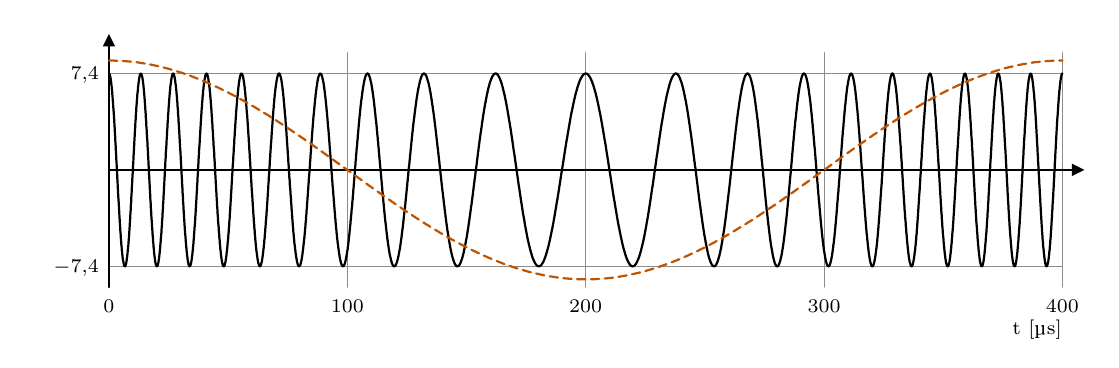
\begin{tikzpicture}[x=0.01985cm,y=-0.01985cm,line cap=round,line join=round]
\useasboundingbox (0,0) rectangle (680,200);
\path[draw=black!45,line width=0.35pt] (52,166) -- (52,16);
\path[draw=black!45,line width=0.35pt] (204.5,166) -- (204.5,16);
\path[draw=black!45,line width=0.35pt] (357,166) -- (357,16);
\path[draw=black!45,line width=0.35pt] (509.5,166) -- (509.5,16);
\path[draw=black!45,line width=0.35pt] (662,166) -- (662,16);
\path[draw=black!45,line width=0.35pt] (52,29.3) -- (662,29.3);
\path[draw=black!45,line width=0.35pt] (52,152.7) -- (662,152.7);
\path[draw=black,line width=0.7pt] (52,91) -- (670,91);
\path[fill=black,draw=none] (676,91) -- (668,87) -- (668,95) -- cycle;
\path[draw=black,line width=0.7pt] (52,166) -- (52,10);
\path[fill=black,draw=none] (52,4) -- (48,12) -- (56,12) -- cycle;
\node[anchor=base,inner sep=0pt,font=\scriptsize] at (52,182) {0};
\node[anchor=base,inner sep=0pt,font=\scriptsize] at (204.5,182) {100};
\node[anchor=base,inner sep=0pt,font=\scriptsize] at (357,182) {200};
\node[anchor=base,inner sep=0pt,font=\scriptsize] at (509.5,182) {300};
\node[anchor=base,inner sep=0pt,font=\scriptsize] at (662,182) {400};
\node[anchor=base east,inner sep=0pt,font=\scriptsize] at (46,33.3) {7,4};
\node[anchor=base east,inner sep=0pt,font=\scriptsize] at (46,156.7) {$-$7,4};
\node[anchor=base east,inner sep=0pt,font=\scriptsize] at (662,196) {t [\textmu{}s]};
\path[draw=black,line width=0.8pt] (52,29.3) -- (52.2,29.4) -- (52.3,29.6) -- (52.5,29.9) -- (52.6,30.4) -- (52.8,31) -- (52.9,31.8) -- (53.1,32.7) -- (53.2,33.7) -- (53.4,34.8) -- (53.5,36.1) -- (53.7,37.4) -- (53.8,38.9) -- (54,40.5) -- (54.1,42.3) -- (54.3,44.1) -- (54.4,46) -- (54.6,48.1) -- (54.7,50.2) -- (54.9,52.4) -- (55.1,54.8) -- (55.2,57.1) -- (55.4,59.6) -- (55.5,62.1) -- (55.7,64.7) -- (55.8,67.4) -- (56,70.1) -- (56.1,72.9) -- (56.3,75.7) -- (56.4,78.5) -- (56.6,81.3) -- (56.7,84.2) -- (56.9,87.1) -- (57,90) -- (57.2,92.9) -- (57.3,95.8) -- (57.5,98.7) -- (57.6,101.6) -- (57.8,104.4) -- (57.9,107.2) -- (58.1,110) -- (58.3,112.8) -- (58.4,115.5) -- (58.6,118.1) -- (58.7,120.7) -- (58.9,123.2) -- (59,125.6) -- (59.2,128) -- (59.3,130.3) -- (59.5,132.5) -- (59.6,134.6) -- (59.8,136.6) -- (59.9,138.5) -- (60.1,140.3) -- (60.2,142) -- (60.4,143.5) -- (60.5,145) -- (60.7,146.3) -- (60.8,147.6) -- (61,148.7) -- (61.2,149.6) -- (61.3,150.5) -- (61.5,151.2) -- (61.6,151.7) -- (61.8,152.2) -- (61.9,152.5) -- (62.1,152.6) -- (62.2,152.7) -- (62.4,152.6) -- (62.5,152.3) -- (62.7,151.9) -- (62.8,151.4) -- (63,150.8) -- (63.1,150) -- (63.3,149.1) -- (63.4,148) -- (63.6,146.9) -- (63.7,145.6) -- (63.9,144.2) -- (64,142.6) -- (64.2,141) -- (64.4,139.3) -- (64.5,137.4) -- (64.7,135.4) -- (64.8,133.4) -- (65,131.2) -- (65.1,129) -- (65.3,126.7) -- (65.4,124.3) -- (65.6,121.8) -- (65.7,119.3) -- (65.9,116.6) -- (66,114) -- (66.2,111.3) -- (66.3,108.5) -- (66.5,105.7) -- (66.6,102.9) -- (66.8,100) -- (66.9,97.2) -- (67.1,94.3) -- (67.3,91.4) -- (67.4,88.5) -- (67.6,85.6) -- (67.7,82.7) -- (67.9,79.9) -- (68,77.1) -- (68.2,74.3) -- (68.3,71.5) -- (68.5,68.8) -- (68.6,66.1) -- (68.8,63.5) -- (68.9,60.9) -- (69.1,58.4) -- (69.2,56) -- (69.4,53.7) -- (69.5,51.4) -- (69.7,49.2) -- (69.8,47.2) -- (70,45.2) -- (70.1,43.3) -- (70.3,41.5) -- (70.5,39.8) -- (70.6,38.3) -- (70.8,36.9) -- (70.9,35.5) -- (71.1,34.3) -- (71.2,33.3) -- (71.4,32.3) -- (71.5,31.5) -- (71.7,30.8) -- (71.8,30.2) -- (72,29.8) -- (72.1,29.5) -- (72.3,29.4) -- (72.4,29.3) -- (72.6,29.5) -- (72.7,29.7) -- (72.9,30.1) -- (73,30.6) -- (73.2,31.2) -- (73.4,32) -- (73.5,32.9) -- (73.7,34) -- (73.8,35.1) -- (74,36.4) -- (74.1,37.8) -- (74.3,39.3) -- (74.4,40.9) -- (74.6,42.7) -- (74.7,44.5) -- (74.9,46.5) -- (75,48.5) -- (75.2,50.6) -- (75.3,52.8) -- (75.5,55.1) -- (75.6,57.5) -- (75.8,60) -- (75.9,62.5) -- (76.1,65.1) -- (76.2,67.7) -- (76.4,70.4) -- (76.6,73.1) -- (76.7,75.9) -- (76.9,78.7) -- (77,81.5) -- (77.2,84.4) -- (77.3,87.2) -- (77.5,90.1) -- (77.6,93) -- (77.8,95.9) -- (77.9,98.7) -- (78.1,101.6) -- (78.2,104.4) -- (78.4,107.2) -- (78.5,109.9) -- (78.7,112.6) -- (78.8,115.3) -- (79,117.9) -- (79.1,120.4) -- (79.3,122.9) -- (79.5,125.3) -- (79.6,127.7) -- (79.8,130) -- (79.9,132.1) -- (80.1,134.2) -- (80.2,136.2) -- (80.4,138.1) -- (80.5,139.9) -- (80.7,141.6) -- (80.8,143.2) -- (81,144.7) -- (81.1,146) -- (81.3,147.2) -- (81.4,148.4) -- (81.6,149.3) -- (81.7,150.2) -- (81.9,150.9) -- (82,151.6) -- (82.2,152) -- (82.3,152.4) -- (82.5,152.6) -- (82.7,152.7) -- (82.8,152.6) -- (83,152.4) -- (83.1,152.1) -- (83.3,151.7) -- (83.4,151.1) -- (83.6,150.4) -- (83.7,149.6) -- (83.9,148.6) -- (84,147.5) -- (84.2,146.3) -- (84.3,145) -- (84.5,143.6) -- (84.6,142) -- (84.8,140.4) -- (84.9,138.6) -- (85.1,136.7) -- (85.2,134.8) -- (85.4,132.7) -- (85.6,130.6) -- (85.7,128.3) -- (85.9,126) -- (86,123.7) -- (86.2,121.2) -- (86.3,118.7) -- (86.5,116.1) -- (86.6,113.5) -- (86.8,110.8) -- (86.9,108.1) -- (87.1,105.4) -- (87.2,102.6) -- (87.4,99.8) -- (87.5,97) -- (87.7,94.1) -- (87.8,91.3) -- (88,88.5) -- (88.1,85.6) -- (88.3,82.8) -- (88.4,80) -- (88.6,77.2) -- (88.8,74.5) -- (88.9,71.7) -- (89.1,69.1) -- (89.2,66.4) -- (89.4,63.9) -- (89.5,61.4) -- (89.7,58.9) -- (89.8,56.5) -- (90,54.2) -- (90.1,52) -- (90.3,49.8) -- (90.4,47.8) -- (90.6,45.8) -- (90.7,43.9) -- (90.9,42.1) -- (91,40.5) -- (91.2,38.9) -- (91.3,37.4) -- (91.5,36.1) -- (91.7,34.9) -- (91.8,33.8) -- (92,32.8) -- (92.1,31.9) -- (92.3,31.2) -- (92.4,30.5) -- (92.6,30) -- (92.7,29.7) -- (92.9,29.4) -- (93,29.3) -- (93.2,29.4) -- (93.3,29.5) -- (93.5,29.8) -- (93.6,30.2) -- (93.8,30.7) -- (93.9,31.4) -- (94.1,32.2) -- (94.2,33.1) -- (94.4,34.1) -- (94.5,35.3) -- (94.7,36.5) -- (94.9,37.9) -- (95,39.4) -- (95.2,41) -- (95.3,42.7) -- (95.5,44.5) -- (95.6,46.4) -- (95.8,48.3) -- (95.9,50.4) -- (96.1,52.6) -- (96.2,54.8) -- (96.4,57.1) -- (96.5,59.5) -- (96.7,61.9) -- (96.8,64.4) -- (97,67) -- (97.1,69.6) -- (97.3,72.3) -- (97.4,74.9) -- (97.6,77.7) -- (97.8,80.4) -- (97.9,83.2) -- (98.1,86) -- (98.2,88.8) -- (98.4,91.6) -- (98.5,94.4) -- (98.7,97.1) -- (98.8,99.9) -- (99,102.7) -- (99.1,105.4) -- (99.3,108.1) -- (99.4,110.8) -- (99.6,113.4) -- (99.7,116) -- (99.9,118.5) -- (100,121) -- (100.2,123.4) -- (100.3,125.7) -- (100.5,128) -- (100.6,130.2) -- (100.8,132.3) -- (101,134.3) -- (101.1,136.2) -- (101.3,138.1) -- (101.4,139.8) -- (101.6,141.5) -- (101.7,143) -- (101.9,144.5) -- (102,145.8) -- (102.2,147) -- (102.3,148.1) -- (102.5,149.1) -- (102.6,150) -- (102.8,150.7) -- (102.9,151.4) -- (103.1,151.9) -- (103.2,152.3) -- (103.4,152.5) -- (103.5,152.6) -- (103.7,152.7) -- (103.9,152.5) -- (104,152.3) -- (104.2,151.9) -- (104.3,151.5) -- (104.5,150.8) -- (104.6,150.1) -- (104.8,149.3) -- (104.9,148.3) -- (105.1,147.2) -- (105.2,146) -- (105.4,144.7) -- (105.5,143.3) -- (105.7,141.8) -- (105.8,140.2) -- (106,138.5) -- (106.1,136.7) -- (106.3,134.8) -- (106.4,132.8) -- (106.6,130.7) -- (106.7,128.6) -- (106.9,126.4) -- (107.1,124.1) -- (107.2,121.7) -- (107.4,119.3) -- (107.5,116.8) -- (107.7,114.3) -- (107.8,111.7) -- (108,109.1) -- (108.1,106.5) -- (108.3,103.8) -- (108.4,101.1) -- (108.6,98.4) -- (108.7,95.7) -- (108.9,92.9) -- (109,90.2) -- (109.2,87.4) -- (109.3,84.7) -- (109.5,82) -- (109.6,79.3) -- (109.8,76.6) -- (110,74) -- (110.1,71.3) -- (110.3,68.8) -- (110.4,66.2) -- (110.6,63.8) -- (110.7,61.3) -- (110.9,59) -- (111,56.7) -- (111.2,54.4) -- (111.3,52.3) -- (111.5,50.2) -- (111.6,48.2) -- (111.8,46.3) -- (111.9,44.4) -- (112.1,42.7) -- (112.2,41) -- (112.4,39.5) -- (112.5,38) -- (112.7,36.7) -- (112.8,35.5) -- (113,34.3) -- (113.2,33.3) -- (113.3,32.4) -- (113.5,31.6) -- (113.6,30.9) -- (113.8,30.4) -- (113.9,29.9) -- (114.1,29.6) -- (114.2,29.4) -- (114.4,29.3) -- (114.5,29.4) -- (114.7,29.5) -- (114.8,29.8) -- (115,30.2) -- (115.1,30.7) -- (115.3,31.3) -- (115.4,32.1) -- (115.6,32.9) -- (115.7,33.9) -- (115.9,35) -- (116.1,36.1) -- (116.2,37.4) -- (116.4,38.8) -- (116.5,40.3) -- (116.7,41.9) -- (116.8,43.6) -- (117,45.3) -- (117.1,47.2) -- (117.3,49.1) -- (117.4,51.1) -- (117.6,53.2) -- (117.7,55.4) -- (117.9,57.6) -- (118,59.9) -- (118.2,62.3) -- (118.3,64.7) -- (118.5,67.1) -- (118.6,69.6) -- (118.8,72.2) -- (118.9,74.8) -- (119.1,77.4) -- (119.3,80) -- (119.4,82.6) -- (119.6,85.3) -- (119.7,88) -- (119.9,90.6) -- (120,93.3) -- (120.2,96) -- (120.3,98.7) -- (120.5,101.3) -- (120.6,103.9) -- (120.8,106.5) -- (120.9,109.1) -- (121.1,111.6) -- (121.2,114.1) -- (121.4,116.6) -- (121.5,119) -- (121.7,121.3) -- (121.8,123.6) -- (122,125.9) -- (122.2,128) -- (122.3,130.1) -- (122.5,132.1) -- (122.6,134.1) -- (122.8,136) -- (122.9,137.7) -- (123.1,139.4) -- (123.2,141) -- (123.4,142.5) -- (123.5,143.9) -- (123.7,145.2) -- (123.8,146.5) -- (124,147.6) -- (124.1,148.6) -- (124.3,149.5) -- (124.4,150.3) -- (124.6,150.9) -- (124.7,151.5) -- (124.9,152) -- (125,152.3) -- (125.2,152.5) -- (125.4,152.7) -- (125.5,152.7) -- (125.7,152.5) -- (125.8,152.3) -- (126,152) -- (126.1,151.5) -- (126.3,151) -- (126.4,150.3) -- (126.6,149.6) -- (126.7,148.7) -- (126.9,147.7) -- (127,146.6) -- (127.2,145.4) -- (127.3,144.1) -- (127.5,142.7) -- (127.6,141.3) -- (127.8,139.7) -- (127.9,138.1) -- (128.1,136.3) -- (128.3,134.5) -- (128.4,132.6) -- (128.6,130.6) -- (128.7,128.6) -- (128.9,126.5) -- (129,124.3) -- (129.2,122.1) -- (129.3,119.8) -- (129.5,117.4) -- (129.6,115.1) -- (129.8,112.6) -- (129.9,110.2) -- (130.1,107.7) -- (130.2,105.2) -- (130.4,102.6) -- (130.5,100) -- (130.7,97.5) -- (130.8,94.9) -- (131,92.3) -- (131.1,89.7) -- (131.3,87.1) -- (131.5,84.5) -- (131.6,81.9) -- (131.8,79.3) -- (131.9,76.8) -- (132.1,74.3) -- (132.2,71.8) -- (132.4,69.3) -- (132.5,66.9) -- (132.7,64.6) -- (132.8,62.3) -- (133,60) -- (133.1,57.8) -- (133.3,55.6) -- (133.4,53.6) -- (133.6,51.5) -- (133.7,49.6) -- (133.9,47.7) -- (134,45.9) -- (134.2,44.2) -- (134.4,42.6) -- (134.5,41) -- (134.7,39.5) -- (134.8,38.2) -- (135,36.9) -- (135.1,35.7) -- (135.3,34.6) -- (135.4,33.6) -- (135.6,32.7) -- (135.7,31.9) -- (135.9,31.2) -- (136,30.7) -- (136.2,30.2) -- (136.3,29.8) -- (136.5,29.5) -- (136.6,29.4) -- (136.8,29.3) -- (136.9,29.4) -- (137.1,29.5) -- (137.2,29.8) -- (137.4,30.2) -- (137.6,30.6) -- (137.7,31.2) -- (137.9,31.9) -- (138,32.7) -- (138.2,33.6) -- (138.3,34.5) -- (138.5,35.6) -- (138.6,36.8) -- (138.8,38) -- (138.9,39.4) -- (139.1,40.8) -- (139.2,42.3) -- (139.4,43.9) -- (139.5,45.6) -- (139.7,47.4) -- (139.8,49.2) -- (140,51.1) -- (140.1,53.1) -- (140.3,55.1) -- (140.5,57.2) -- (140.6,59.3) -- (140.8,61.5) -- (140.9,63.7) -- (141.1,66) -- (141.2,68.4) -- (141.4,70.7) -- (141.5,73.1) -- (141.7,75.6) -- (141.8,78) -- (142,80.5) -- (142.1,83) -- (142.3,85.5) -- (142.4,88) -- (142.6,90.5) -- (142.7,93) -- (142.9,95.5) -- (143,98) -- (143.2,100.5) -- (143.3,103) -- (143.5,105.4) -- (143.7,107.9) -- (143.8,110.2) -- (144,112.6) -- (144.1,114.9) -- (144.3,117.2) -- (144.4,119.5) -- (144.6,121.7) -- (144.7,123.8) -- (144.9,125.9) -- (145,127.9) -- (145.2,129.9) -- (145.3,131.8) -- (145.5,133.6) -- (145.6,135.4) -- (145.8,137.1) -- (145.9,138.7) -- (146.1,140.2) -- (146.2,141.7) -- (146.4,143.1) -- (146.6,144.3) -- (146.7,145.5) -- (146.9,146.7) -- (147,147.7) -- (147.2,148.6) -- (147.3,149.4) -- (147.5,150.2) -- (147.6,150.8) -- (147.8,151.4) -- (147.9,151.8) -- (148.1,152.2) -- (148.2,152.4) -- (148.4,152.6) -- (148.5,152.7) -- (148.7,152.6) -- (148.8,152.5) -- (149,152.3) -- (149.1,151.9) -- (149.3,151.5) -- (149.4,151) -- (149.6,150.3) -- (149.8,149.6) -- (149.9,148.8) -- (150.1,147.9) -- (150.2,146.9) -- (150.4,145.9) -- (150.5,144.7) -- (150.7,143.5) -- (150.8,142.1) -- (151,140.7) -- (151.1,139.2) -- (151.3,137.7) -- (151.4,136.1) -- (151.6,134.4) -- (151.7,132.6) -- (151.9,130.8) -- (152,128.9) -- (152.2,126.9) -- (152.3,124.9) -- (152.5,122.8) -- (152.7,120.7) -- (152.8,118.6) -- (153,116.4) -- (153.1,114.2) -- (153.3,111.9) -- (153.4,109.6) -- (153.6,107.3) -- (153.7,104.9) -- (153.9,102.6) -- (154,100.2) -- (154.2,97.8) -- (154.3,95.4) -- (154.5,93) -- (154.6,90.5) -- (154.8,88.1) -- (154.9,85.7) -- (155.1,83.3) -- (155.2,80.9) -- (155.4,78.6) -- (155.5,76.2) -- (155.7,73.9) -- (155.9,71.6) -- (156,69.4) -- (156.2,67.1) -- (156.3,64.9) -- (156.5,62.8) -- (156.6,60.7) -- (156.8,58.6) -- (156.9,56.6) -- (157.1,54.6) -- (157.2,52.7) -- (157.4,50.9) -- (157.5,49.1) -- (157.7,47.4) -- (157.8,45.7) -- (158,44.1) -- (158.1,42.6) -- (158.3,41.2) -- (158.4,39.8) -- (158.6,38.5) -- (158.8,37.3) -- (158.9,36.2) -- (159.1,35.1) -- (159.2,34.2) -- (159.4,33.3) -- (159.5,32.5) -- (159.7,31.8) -- (159.8,31.2) -- (160,30.7) -- (160.1,30.2) -- (160.3,29.9) -- (160.4,29.6) -- (160.6,29.4) -- (160.7,29.3) -- (160.9,29.3) -- (161,29.4) -- (161.2,29.6) -- (161.3,29.9) -- (161.5,30.3) -- (161.6,30.7) -- (161.8,31.3) -- (162,31.9) -- (162.1,32.6) -- (162.3,33.4) -- (162.4,34.3) -- (162.6,35.3) -- (162.7,36.3) -- (162.9,37.4) -- (163,38.6) -- (163.2,39.9) -- (163.3,41.2) -- (163.5,42.6) -- (163.6,44.1) -- (163.8,45.7) -- (163.9,47.3) -- (164.1,49) -- (164.2,50.7) -- (164.4,52.5) -- (164.5,54.3) -- (164.7,56.2) -- (164.9,58.2) -- (165,60.2) -- (165.2,62.2) -- (165.3,64.3) -- (165.5,66.4) -- (165.6,68.5) -- (165.8,70.7) -- (165.9,72.9) -- (166.1,75.1) -- (166.2,77.3) -- (166.4,79.6) -- (166.5,81.9) -- (166.7,84.2) -- (166.8,86.5) -- (167,88.8) -- (167.1,91.1) -- (167.3,93.4) -- (167.4,95.6) -- (167.6,97.9) -- (167.7,100.2) -- (167.9,102.5) -- (168.1,104.7) -- (168.2,106.9) -- (168.4,109.1) -- (168.5,111.3) -- (168.7,113.5) -- (168.8,115.6) -- (169,117.7) -- (169.1,119.7) -- (169.3,121.7) -- (169.4,123.7) -- (169.6,125.6) -- (169.7,127.4) -- (169.9,129.2) -- (170,131) -- (170.2,132.7) -- (170.3,134.3) -- (170.5,135.9) -- (170.6,137.5) -- (170.8,138.9) -- (171,140.3) -- (171.1,141.6) -- (171.3,142.9) -- (171.4,144.1) -- (171.6,145.2) -- (171.7,146.2) -- (171.9,147.2) -- (172,148.1) -- (172.2,148.9) -- (172.3,149.6) -- (172.5,150.3) -- (172.6,150.9) -- (172.8,151.4) -- (172.9,151.8) -- (173.1,152.1) -- (173.2,152.4) -- (173.4,152.6) -- (173.5,152.7) -- (173.7,152.7) -- (173.8,152.6) -- (174,152.4) -- (174.2,152.2) -- (174.3,151.9) -- (174.5,151.5) -- (174.6,151) -- (174.8,150.5) -- (174.9,149.9) -- (175.1,149.2) -- (175.2,148.4) -- (175.4,147.5) -- (175.5,146.6) -- (175.7,145.6) -- (175.8,144.5) -- (176,143.4) -- (176.1,142.2) -- (176.3,140.9) -- (176.4,139.6) -- (176.6,138.2) -- (176.7,136.8) -- (176.9,135.2) -- (177.1,133.7) -- (177.2,132.1) -- (177.4,130.4) -- (177.5,128.7) -- (177.7,126.9) -- (177.8,125.1) -- (178,123.2) -- (178.1,121.3) -- (178.3,119.4) -- (178.4,117.4) -- (178.6,115.4) -- (178.7,113.4) -- (178.9,111.4) -- (179,109.3) -- (179.2,107.2) -- (179.3,105.1) -- (179.5,102.9) -- (179.6,100.8) -- (179.8,98.6) -- (179.9,96.4) -- (180.1,94.3) -- (180.3,92.1) -- (180.4,89.9) -- (180.6,87.7) -- (180.7,85.6) -- (180.9,83.4) -- (181,81.3) -- (181.2,79.1) -- (181.3,77) -- (181.5,74.9) -- (181.6,72.8) -- (181.8,70.8) -- (181.9,68.8) -- (182.1,66.8) -- (182.2,64.8) -- (182.4,62.9) -- (182.5,61) -- (182.7,59.1) -- (182.8,57.3) -- (183,55.5) -- (183.2,53.8) -- (183.3,52.1) -- (183.5,50.4) -- (183.6,48.8) -- (183.8,47.3) -- (183.9,45.8) -- (184.1,44.4) -- (184.2,43) -- (184.4,41.7) -- (184.5,40.4) -- (184.7,39.3) -- (184.8,38.1) -- (185,37.1) -- (185.1,36.1) -- (185.3,35.1) -- (185.4,34.3) -- (185.6,33.5) -- (185.7,32.7) -- (185.9,32.1) -- (186,31.5) -- (186.2,31) -- (186.4,30.5) -- (186.5,30.1) -- (186.7,29.8) -- (186.8,29.6) -- (187,29.4) -- (187.1,29.4) -- (187.3,29.3) -- (187.4,29.4) -- (187.6,29.5) -- (187.7,29.7) -- (187.9,30) -- (188,30.3) -- (188.2,30.7) -- (188.3,31.2) -- (188.5,31.8) -- (188.6,32.4) -- (188.8,33.1) -- (188.9,33.8) -- (189.1,34.6) -- (189.3,35.5) -- (189.4,36.5) -- (189.6,37.5) -- (189.7,38.5) -- (189.9,39.7) -- (190,40.9) -- (190.2,42.1) -- (190.3,43.4) -- (190.5,44.7) -- (190.6,46.1) -- (190.8,47.6) -- (190.9,49.1) -- (191.1,50.6) -- (191.2,52.2) -- (191.4,53.8) -- (191.5,55.5) -- (191.7,57.2) -- (191.8,59) -- (192,60.7) -- (192.1,62.6) -- (192.3,64.4) -- (192.5,66.3) -- (192.6,68.2) -- (192.8,70.1) -- (192.9,72) -- (193.1,74) -- (193.2,76) -- (193.4,78) -- (193.5,80) -- (193.7,82) -- (193.8,84) -- (194,86) -- (194.1,88.1) -- (194.3,90.1) -- (194.4,92.2) -- (194.6,94.2) -- (194.7,96.2) -- (194.9,98.3) -- (195,100.3) -- (195.2,102.3) -- (195.4,104.3) -- (195.5,106.2) -- (195.7,108.2) -- (195.8,110.1) -- (196,112) -- (196.1,113.9) -- (196.3,115.8) -- (196.4,117.6) -- (196.6,119.4) -- (196.7,121.2) -- (196.9,122.9) -- (197,124.6) -- (197.2,126.3) -- (197.3,127.9) -- (197.5,129.5) -- (197.6,131.1) -- (197.8,132.6) -- (197.9,134) -- (198.1,135.4) -- (198.2,136.8) -- (198.4,138.1) -- (198.6,139.4) -- (198.7,140.6) -- (198.9,141.8) -- (199,142.9) -- (199.2,143.9) -- (199.3,144.9) -- (199.5,145.8) -- (199.6,146.7) -- (199.8,147.5) -- (199.9,148.3) -- (200.1,149) -- (200.2,149.6) -- (200.4,150.2) -- (200.5,150.8) -- (200.7,151.2) -- (200.8,151.6) -- (201,151.9) -- (201.1,152.2) -- (201.3,152.4) -- (201.5,152.6) -- (201.6,152.6) -- (201.8,152.7) -- (201.9,152.6) -- (202.1,152.5) -- (202.2,152.4) -- (202.4,152.1) -- (202.5,151.8) -- (202.7,151.5) -- (202.8,151.1) -- (203,150.6) -- (203.1,150.1) -- (203.3,149.5) -- (203.4,148.8) -- (203.6,148.1) -- (203.7,147.4) -- (203.9,146.5) -- (204,145.7) -- (204.2,144.7) -- (204.3,143.8) -- (204.5,142.7) -- (204.7,141.7) -- (204.8,140.5) -- (205,139.4) -- (205.1,138.1) -- (205.3,136.9) -- (205.4,135.6) -- (205.6,134.2) -- (205.7,132.8) -- (205.9,131.4) -- (206,129.9) -- (206.2,128.4) -- (206.3,126.8) -- (206.5,125.3) -- (206.6,123.7) -- (206.8,122) -- (206.9,120.4) -- (207.1,118.7) -- (207.2,116.9) -- (207.4,115.2) -- (207.6,113.4) -- (207.7,111.6) -- (207.9,109.8) -- (208,108) -- (208.2,106.2) -- (208.3,104.3) -- (208.5,102.5) -- (208.6,100.6) -- (208.8,98.7) -- (208.9,96.8) -- (209.1,95) -- (209.2,93.1) -- (209.4,91.2) -- (209.5,89.3) -- (209.7,87.4) -- (209.8,85.5) -- (210,83.7) -- (210.1,81.8) -- (210.3,79.9) -- (210.4,78.1) -- (210.6,76.3) -- (210.8,74.4) -- (210.9,72.7) -- (211.1,70.9) -- (211.2,69.1) -- (211.4,67.4) -- (211.5,65.7) -- (211.7,64) -- (211.8,62.3) -- (212,60.7) -- (212.1,59.1) -- (212.3,57.5) -- (212.4,55.9) -- (212.6,54.4) -- (212.7,53) -- (212.9,51.5) -- (213,50.1) -- (213.2,48.7) -- (213.3,47.4) -- (213.5,46.1) -- (213.7,44.9) -- (213.8,43.7) -- (214,42.5) -- (214.1,41.4) -- (214.3,40.3) -- (214.4,39.3) -- (214.6,38.3) -- (214.7,37.4) -- (214.9,36.5) -- (215,35.7) -- (215.2,34.9) -- (215.3,34.2) -- (215.5,33.5) -- (215.6,32.8) -- (215.8,32.3) -- (215.9,31.7) -- (216.1,31.2) -- (216.2,30.8) -- (216.4,30.5) -- (216.5,30.1) -- (216.7,29.9) -- (216.9,29.7) -- (217,29.5) -- (217.2,29.4) -- (217.3,29.3) -- (217.5,29.3) -- (217.6,29.4) -- (217.8,29.5) -- (217.9,29.7) -- (218.1,29.9) -- (218.2,30.1) -- (218.4,30.4) -- (218.5,30.8) -- (218.7,31.2) -- (218.8,31.7) -- (219,32.2) -- (219.1,32.8) -- (219.3,33.4) -- (219.4,34.1) -- (219.6,34.8) -- (219.8,35.5) -- (219.9,36.3) -- (220.1,37.2) -- (220.2,38.1) -- (220.4,39) -- (220.5,40) -- (220.7,41) -- (220.8,42.1) -- (221,43.2) -- (221.1,44.3) -- (221.3,45.5) -- (221.4,46.7) -- (221.6,47.9) -- (221.7,49.2) -- (221.9,50.5) -- (222,51.9) -- (222.2,53.3) -- (222.3,54.7) -- (222.5,56.1) -- (222.6,57.6) -- (222.8,59.1) -- (223,60.6) -- (223.1,62.1) -- (223.3,63.7) -- (223.4,65.3) -- (223.6,66.9) -- (223.7,68.5) -- (223.9,70.1) -- (224,71.8) -- (224.2,73.4) -- (224.3,75.1) -- (224.5,76.8) -- (224.6,78.5) -- (224.8,80.2) -- (224.9,81.9) -- (225.1,83.6) -- (225.2,85.3) -- (225.4,87.1) -- (225.5,88.8) -- (225.7,90.5) -- (225.9,92.2) -- (226,94) -- (226.2,95.7) -- (226.3,97.4) -- (226.5,99.1) -- (226.6,100.8) -- (226.8,102.5) -- (226.9,104.2) -- (227.1,105.9) -- (227.2,107.5) -- (227.4,109.2) -- (227.5,110.8) -- (227.7,112.4) -- (227.8,114) -- (228,115.6) -- (228.1,117.1) -- (228.3,118.7) -- (228.4,120.2) -- (228.6,121.6) -- (228.7,123.1) -- (228.9,124.5) -- (229.1,126) -- (229.2,127.3) -- (229.4,128.7) -- (229.5,130) -- (229.7,131.3) -- (229.8,132.6) -- (230,133.8) -- (230.1,135) -- (230.3,136.2) -- (230.4,137.3) -- (230.6,138.4) -- (230.7,139.4) -- (230.9,140.5) -- (231,141.4) -- (231.2,142.4) -- (231.3,143.3) -- (231.5,144.2) -- (231.6,145) -- (231.8,145.8) -- (232,146.5) -- (232.1,147.2) -- (232.3,147.9) -- (232.4,148.5) -- (232.6,149.1) -- (232.7,149.6) -- (232.9,150.1) -- (233,150.6) -- (233.2,151) -- (233.3,151.3) -- (233.5,151.7) -- (233.6,151.9) -- (233.8,152.2) -- (233.9,152.4) -- (234.1,152.5) -- (234.2,152.6) -- (234.4,152.7) -- (234.5,152.7) -- (234.7,152.6) -- (234.8,152.6) -- (235,152.4) -- (235.2,152.3) -- (235.3,152.1) -- (235.5,151.8) -- (235.6,151.5) -- (235.8,151.2) -- (235.9,150.8) -- (236.1,150.4) -- (236.2,150) -- (236.4,149.5) -- (236.5,148.9) -- (236.7,148.3) -- (236.8,147.7) -- (237,147.1) -- (237.1,146.4) -- (237.3,145.7) -- (237.4,144.9) -- (237.6,144.1) -- (237.7,143.2) -- (237.9,142.4) -- (238.1,141.5) -- (238.2,140.5) -- (238.4,139.5) -- (238.5,138.5) -- (238.7,137.5) -- (238.8,136.4) -- (239,135.3) -- (239.1,134.2) -- (239.3,133.1) -- (239.4,131.9) -- (239.6,130.7) -- (239.7,129.4) -- (239.9,128.2) -- (240,126.9) -- (240.2,125.6) -- (240.3,124.3) -- (240.5,122.9) -- (240.6,121.5) -- (240.8,120.2) -- (240.9,118.8) -- (241.1,117.3) -- (241.3,115.9) -- (241.4,114.4) -- (241.6,113) -- (241.7,111.5) -- (241.9,110) -- (242,108.5) -- (242.2,107) -- (242.3,105.5) -- (242.5,103.9) -- (242.6,102.4) -- (242.8,100.9) -- (242.9,99.3) -- (243.1,97.8) -- (243.2,96.2) -- (243.4,94.7) -- (243.5,93.1) -- (243.7,91.5) -- (243.8,90) -- (244,88.4) -- (244.2,86.9) -- (244.3,85.3) -- (244.5,83.8) -- (244.6,82.3) -- (244.8,80.7) -- (244.9,79.2) -- (245.1,77.7) -- (245.2,76.2) -- (245.4,74.7) -- (245.5,73.2) -- (245.7,71.7) -- (245.8,70.3) -- (246,68.8) -- (246.1,67.4) -- (246.3,66) -- (246.4,64.6) -- (246.6,63.2) -- (246.7,61.9) -- (246.9,60.5) -- (247,59.2) -- (247.2,57.9) -- (247.4,56.7) -- (247.5,55.4) -- (247.7,54.2) -- (247.8,53) -- (248,51.8) -- (248.1,50.6) -- (248.3,49.5) -- (248.4,48.4) -- (248.6,47.3) -- (248.7,46.2) -- (248.9,45.2) -- (249,44.2) -- (249.2,43.3) -- (249.3,42.3) -- (249.5,41.4) -- (249.6,40.5) -- (249.8,39.7) -- (249.9,38.9) -- (250.1,38.1) -- (250.3,37.3) -- (250.4,36.6) -- (250.6,35.9) -- (250.7,35.3) -- (250.9,34.6) -- (251,34) -- (251.2,33.5) -- (251.3,33) -- (251.5,32.5) -- (251.6,32) -- (251.8,31.6) -- (251.9,31.2) -- (252.1,30.9) -- (252.2,30.6) -- (252.4,30.3) -- (252.5,30.1) -- (252.7,29.8) -- (252.8,29.7) -- (253,29.5) -- (253.1,29.4) -- (253.3,29.4) -- (253.5,29.3) -- (253.6,29.3) -- (253.8,29.4) -- (253.9,29.5) -- (254.1,29.6) -- (254.2,29.7) -- (254.4,29.9) -- (254.5,30.1) -- (254.7,30.3) -- (254.8,30.6) -- (255,30.9) -- (255.1,31.3) -- (255.3,31.6) -- (255.4,32.1) -- (255.6,32.5) -- (255.7,33) -- (255.9,33.5) -- (256,34) -- (256.2,34.6) -- (256.4,35.2) -- (256.5,35.8) -- (256.7,36.5) -- (256.8,37.2) -- (257,37.9) -- (257.1,38.6) -- (257.3,39.4) -- (257.4,40.2) -- (257.6,41) -- (257.7,41.9) -- (257.9,42.8) -- (258,43.7) -- (258.2,44.6) -- (258.3,45.5) -- (258.5,46.5) -- (258.6,47.5) -- (258.8,48.5) -- (258.9,49.6) -- (259.1,50.6) -- (259.2,51.7) -- (259.4,52.8) -- (259.6,54) -- (259.7,55.1) -- (259.9,56.3) -- (260,57.4) -- (260.2,58.6) -- (260.3,59.8) -- (260.5,61.1) -- (260.6,62.3) -- (260.8,63.6) -- (260.9,64.8) -- (261.1,66.1) -- (261.2,67.4) -- (261.4,68.7) -- (261.5,70) -- (261.7,71.3) -- (261.8,72.7) -- (262,74) -- (262.1,75.3) -- (262.3,76.7) -- (262.5,78.1) -- (262.6,79.4) -- (262.8,80.8) -- (262.9,82.2) -- (263.1,83.5) -- (263.2,84.9) -- (263.4,86.3) -- (263.5,87.7) -- (263.7,89.1) -- (263.8,90.4) -- (264,91.8) -- (264.1,93.2) -- (264.3,94.6) -- (264.4,96) -- (264.6,97.3) -- (264.7,98.7) -- (264.9,100.1) -- (265,101.4) -- (265.2,102.8) -- (265.3,104.1) -- (265.5,105.4) -- (265.7,106.8) -- (265.8,108.1) -- (266,109.4) -- (266.1,110.7) -- (266.3,112) -- (266.4,113.2) -- (266.6,114.5) -- (266.7,115.8) -- (266.9,117) -- (267,118.2) -- (267.2,119.4) -- (267.3,120.6) -- (267.5,121.8) -- (267.6,123) -- (267.8,124.1) -- (267.9,125.2) -- (268.1,126.3) -- (268.2,127.4) -- (268.4,128.5) -- (268.5,129.6) -- (268.7,130.6) -- (268.9,131.6) -- (269,132.6) -- (269.2,133.6) -- (269.3,134.6) -- (269.5,135.5) -- (269.6,136.4) -- (269.8,137.3) -- (269.9,138.2) -- (270.1,139) -- (270.2,139.9) -- (270.4,140.7) -- (270.5,141.4) -- (270.7,142.2) -- (270.8,142.9) -- (271,143.6) -- (271.1,144.3) -- (271.3,144.9) -- (271.4,145.6) -- (271.6,146.2) -- (271.8,146.8) -- (271.9,147.3) -- (272.1,147.8) -- (272.2,148.3) -- (272.4,148.8) -- (272.5,149.2) -- (272.7,149.7) -- (272.8,150) -- (273,150.4) -- (273.1,150.8) -- (273.3,151.1) -- (273.4,151.3) -- (273.6,151.6) -- (273.7,151.8) -- (273.9,152) -- (274,152.2) -- (274.2,152.3) -- (274.3,152.5) -- (274.5,152.6) -- (274.7,152.6) -- (274.8,152.7) -- (275,152.7) -- (275.1,152.6) -- (275.3,152.6) -- (275.4,152.5) -- (275.6,152.4) -- (275.7,152.3) -- (275.9,152.2) -- (276,152) -- (276.2,151.8) -- (276.3,151.5) -- (276.5,151.3) -- (276.6,151) -- (276.8,150.7) -- (276.9,150.4) -- (277.1,150) -- (277.2,149.6) -- (277.4,149.2) -- (277.5,148.8) -- (277.7,148.3) -- (277.9,147.8) -- (278,147.3) -- (278.2,146.8) -- (278.3,146.2) -- (278.5,145.7) -- (278.6,145.1) -- (278.8,144.4) -- (278.9,143.8) -- (279.1,143.1) -- (279.2,142.4) -- (279.4,141.7) -- (279.5,141) -- (279.7,140.3) -- (279.8,139.5) -- (280,138.7) -- (280.1,137.9) -- (280.3,137.1) -- (280.4,136.2) -- (280.6,135.4) -- (280.8,134.5) -- (280.9,133.6) -- (281.1,132.7) -- (281.2,131.8) -- (281.4,130.8) -- (281.5,129.9) -- (281.7,128.9) -- (281.8,127.9) -- (282,126.9) -- (282.1,125.9) -- (282.3,124.8) -- (282.4,123.8) -- (282.6,122.7) -- (282.7,121.7) -- (282.9,120.6) -- (283,119.5) -- (283.2,118.4) -- (283.3,117.3) -- (283.5,116.2) -- (283.6,115) -- (283.8,113.9) -- (284,112.7) -- (284.1,111.6) -- (284.3,110.4) -- (284.4,109.3) -- (284.6,108.1) -- (284.7,106.9) -- (284.9,105.7) -- (285,104.5) -- (285.2,103.3) -- (285.3,102.1) -- (285.5,100.9) -- (285.6,99.7) -- (285.8,98.5) -- (285.9,97.3) -- (286.1,96.1) -- (286.2,94.9) -- (286.4,93.7) -- (286.5,92.5) -- (286.7,91.2) -- (286.9,90) -- (287,88.8) -- (287.2,87.6) -- (287.3,86.4) -- (287.5,85.2) -- (287.6,84) -- (287.8,82.8) -- (287.9,81.6) -- (288.1,80.4) -- (288.2,79.2) -- (288.4,78.1) -- (288.5,76.9) -- (288.7,75.7) -- (288.8,74.6) -- (289,73.4) -- (289.1,72.3) -- (289.3,71.1) -- (289.4,70) -- (289.6,68.9) -- (289.7,67.8) -- (289.9,66.7) -- (290.1,65.6) -- (290.2,64.5) -- (290.4,63.5) -- (290.5,62.4) -- (290.7,61.3) -- (290.8,60.3) -- (291,59.3) -- (291.1,58.3) -- (291.3,57.3) -- (291.4,56.3) -- (291.6,55.3) -- (291.7,54.4) -- (291.9,53.4) -- (292,52.5) -- (292.2,51.6) -- (292.3,50.7) -- (292.5,49.8) -- (292.6,49) -- (292.8,48.1) -- (293,47.3) -- (293.1,46.4) -- (293.3,45.6) -- (293.4,44.9) -- (293.6,44.1) -- (293.7,43.3) -- (293.9,42.6) -- (294,41.9) -- (294.2,41.2) -- (294.3,40.5) -- (294.5,39.9) -- (294.6,39.2) -- (294.8,38.6) -- (294.9,38) -- (295.1,37.4) -- (295.2,36.9) -- (295.4,36.3) -- (295.5,35.8) -- (295.7,35.3) -- (295.8,34.8) -- (296,34.3) -- (296.2,33.9) -- (296.3,33.5) -- (296.5,33.1) -- (296.6,32.7) -- (296.8,32.3) -- (296.9,32) -- (297.1,31.6) -- (297.2,31.3) -- (297.4,31.1) -- (297.5,30.8) -- (297.7,30.6) -- (297.8,30.4) -- (298,30.2) -- (298.1,30) -- (298.3,29.8) -- (298.4,29.7) -- (298.6,29.6) -- (298.7,29.5) -- (298.9,29.4) -- (299.1,29.4) -- (299.2,29.3) -- (299.4,29.3) -- (299.5,29.3) -- (299.7,29.4) -- (299.8,29.4) -- (300,29.5) -- (300.1,29.6) -- (300.3,29.7) -- (300.4,29.9) -- (300.6,30) -- (300.7,30.2) -- (300.9,30.4) -- (301,30.6) -- (301.2,30.9) -- (301.3,31.1) -- (301.5,31.4) -- (301.6,31.7) -- (301.8,32) -- (301.9,32.3) -- (302.1,32.7) -- (302.3,33.1) -- (302.4,33.5) -- (302.6,33.9) -- (302.7,34.3) -- (302.9,34.8) -- (303,35.2) -- (303.2,35.7) -- (303.3,36.2) -- (303.5,36.7) -- (303.6,37.3) -- (303.8,37.8) -- (303.9,38.4) -- (304.1,39) -- (304.2,39.6) -- (304.4,40.2) -- (304.5,40.8) -- (304.7,41.5) -- (304.8,42.1) -- (305,42.8) -- (305.2,43.5) -- (305.3,44.2) -- (305.5,45) -- (305.6,45.7) -- (305.8,46.5) -- (305.9,47.2) -- (306.1,48) -- (306.2,48.8) -- (306.4,49.6) -- (306.5,50.4) -- (306.7,51.3) -- (306.8,52.1) -- (307,53) -- (307.1,53.8) -- (307.3,54.7) -- (307.4,55.6) -- (307.6,56.5) -- (307.7,57.4) -- (307.9,58.3) -- (308,59.3) -- (308.2,60.2) -- (308.4,61.1) -- (308.5,62.1) -- (308.7,63.1) -- (308.8,64) -- (309,65) -- (309.1,66) -- (309.3,67) -- (309.4,68) -- (309.6,69) -- (309.7,70) -- (309.9,71) -- (310,72.1) -- (310.2,73.1) -- (310.3,74.1) -- (310.5,75.2) -- (310.6,76.2) -- (310.8,77.3) -- (310.9,78.3) -- (311.1,79.4) -- (311.3,80.4) -- (311.4,81.5) -- (311.6,82.5) -- (311.7,83.6) -- (311.9,84.7) -- (312,85.7) -- (312.2,86.8) -- (312.3,87.9) -- (312.5,88.9) -- (312.6,90) -- (312.8,91.1) -- (312.9,92.1) -- (313.1,93.2) -- (313.2,94.3) -- (313.4,95.3) -- (313.5,96.4) -- (313.7,97.5) -- (313.8,98.5) -- (314,99.6) -- (314.1,100.6) -- (314.3,101.7) -- (314.5,102.7) -- (314.6,103.7) -- (314.8,104.8) -- (314.9,105.8) -- (315.1,106.8) -- (315.2,107.8) -- (315.4,108.9) -- (315.5,109.9) -- (315.7,110.9) -- (315.8,111.9) -- (316,112.9) -- (316.1,113.8) -- (316.3,114.8) -- (316.4,115.8) -- (316.6,116.7) -- (316.7,117.7) -- (316.9,118.6) -- (317,119.6) -- (317.2,120.5) -- (317.4,121.4) -- (317.5,122.3) -- (317.7,123.2) -- (317.8,124.1) -- (318,125) -- (318.1,125.9) -- (318.3,126.7) -- (318.4,127.6) -- (318.6,128.4) -- (318.7,129.2) -- (318.9,130) -- (319,130.8) -- (319.2,131.6) -- (319.3,132.4) -- (319.5,133.2) -- (319.6,133.9) -- (319.8,134.7) -- (319.9,135.4) -- (320.1,136.1) -- (320.2,136.8) -- (320.4,137.5) -- (320.6,138.2) -- (320.7,138.8) -- (320.9,139.5) -- (321,140.1) -- (321.2,140.7) -- (321.3,141.3) -- (321.5,141.9) -- (321.6,142.5) -- (321.8,143) -- (321.9,143.6) -- (322.1,144.1) -- (322.2,144.6) -- (322.4,145.1) -- (322.5,145.6) -- (322.7,146.1) -- (322.8,146.6) -- (323,147) -- (323.1,147.4) -- (323.3,147.8) -- (323.5,148.2) -- (323.6,148.6) -- (323.8,148.9) -- (323.9,149.3) -- (324.1,149.6) -- (324.2,149.9) -- (324.4,150.2) -- (324.5,150.5) -- (324.7,150.8) -- (324.8,151) -- (325,151.2) -- (325.1,151.4) -- (325.3,151.6) -- (325.4,151.8) -- (325.6,152) -- (325.7,152.1) -- (325.9,152.2) -- (326,152.4) -- (326.2,152.4) -- (326.3,152.5) -- (326.5,152.6) -- (326.7,152.6) -- (326.8,152.7) -- (327,152.7) -- (327.1,152.7) -- (327.3,152.6) -- (327.4,152.6) -- (327.6,152.5) -- (327.7,152.5) -- (327.9,152.4) -- (328,152.3) -- (328.2,152.2) -- (328.3,152) -- (328.5,151.9) -- (328.6,151.7) -- (328.8,151.5) -- (328.9,151.3) -- (329.1,151.1) -- (329.2,150.8) -- (329.4,150.6) -- (329.6,150.3) -- (329.7,150) -- (329.9,149.7) -- (330,149.4) -- (330.2,149.1) -- (330.3,148.8) -- (330.5,148.4) -- (330.6,148) -- (330.8,147.6) -- (330.9,147.2) -- (331.1,146.8) -- (331.2,146.4) -- (331.4,145.9) -- (331.5,145.5) -- (331.7,145) -- (331.8,144.5) -- (332,144) -- (332.1,143.5) -- (332.3,142.9) -- (332.4,142.4) -- (332.6,141.8) -- (332.8,141.3) -- (332.9,140.7) -- (333.1,140.1) -- (333.2,139.5) -- (333.4,138.8) -- (333.5,138.2) -- (333.7,137.6) -- (333.8,136.9) -- (334,136.2) -- (334.1,135.5) -- (334.3,134.8) -- (334.4,134.1) -- (334.6,133.4) -- (334.7,132.7) -- (334.9,132) -- (335,131.2) -- (335.2,130.5) -- (335.3,129.7) -- (335.5,128.9) -- (335.7,128.1) -- (335.8,127.3) -- (336,126.5) -- (336.1,125.7) -- (336.3,124.9) -- (336.4,124.1) -- (336.6,123.2) -- (336.7,122.4) -- (336.9,121.5) -- (337,120.6) -- (337.2,119.8) -- (337.3,118.9) -- (337.5,118) -- (337.6,117.1) -- (337.8,116.2) -- (337.9,115.3) -- (338.1,114.4) -- (338.2,113.5) -- (338.4,112.6) -- (338.5,111.6) -- (338.7,110.7) -- (338.9,109.8) -- (339,108.8) -- (339.2,107.9) -- (339.3,106.9) -- (339.5,106) -- (339.6,105) -- (339.8,104.1) -- (339.9,103.1) -- (340.1,102.1) -- (340.2,101.2) -- (340.4,100.2) -- (340.5,99.2) -- (340.7,98.3) -- (340.8,97.3) -- (341,96.3) -- (341.1,95.3) -- (341.3,94.3) -- (341.4,93.4) -- (341.6,92.4) -- (341.8,91.4) -- (341.9,90.4) -- (342.1,89.4) -- (342.2,88.5) -- (342.4,87.5) -- (342.5,86.5) -- (342.7,85.5) -- (342.8,84.6) -- (343,83.6) -- (343.1,82.6) -- (343.3,81.6) -- (343.4,80.7) -- (343.6,79.7) -- (343.7,78.8) -- (343.9,77.8) -- (344,76.8) -- (344.2,75.9) -- (344.3,74.9) -- (344.5,74) -- (344.6,73.1) -- (344.8,72.1) -- (345,71.2) -- (345.1,70.3) -- (345.3,69.4) -- (345.4,68.5) -- (345.6,67.6) -- (345.7,66.7) -- (345.9,65.8) -- (346,64.9) -- (346.2,64) -- (346.3,63.1) -- (346.5,62.3) -- (346.6,61.4) -- (346.8,60.6) -- (346.9,59.7) -- (347.1,58.9) -- (347.2,58) -- (347.4,57.2) -- (347.5,56.4) -- (347.7,55.6) -- (347.8,54.8) -- (348,54) -- (348.2,53.3) -- (348.3,52.5) -- (348.5,51.7) -- (348.6,51) -- (348.8,50.3) -- (348.9,49.5) -- (349.1,48.8) -- (349.2,48.1) -- (349.4,47.4) -- (349.5,46.7) -- (349.7,46.1) -- (349.8,45.4) -- (350,44.8) -- (350.1,44.1) -- (350.3,43.5) -- (350.4,42.9) -- (350.6,42.3) -- (350.7,41.7) -- (350.9,41.1) -- (351.1,40.6) -- (351.2,40) -- (351.4,39.5) -- (351.5,38.9) -- (351.7,38.4) -- (351.8,37.9) -- (352,37.4) -- (352.1,37) -- (352.3,36.5) -- (352.4,36.1) -- (352.6,35.6) -- (352.7,35.2) -- (352.9,34.8) -- (353,34.4) -- (353.2,34) -- (353.3,33.7) -- (353.5,33.3) -- (353.6,33) -- (353.8,32.7) -- (354,32.4) -- (354.1,32.1) -- (354.3,31.8) -- (354.4,31.5) -- (354.6,31.3) -- (354.7,31) -- (354.9,30.8) -- (355,30.6) -- (355.2,30.4) -- (355.3,30.3) -- (355.5,30.1) -- (355.6,29.9) -- (355.8,29.8) -- (355.9,29.7) -- (356.1,29.6) -- (356.2,29.5) -- (356.4,29.5) -- (356.5,29.4) -- (356.7,29.4) -- (356.8,29.3) -- (357,29.3) -- (357.2,29.3) -- (357.3,29.4) -- (357.5,29.4) -- (357.6,29.5) -- (357.8,29.5) -- (357.9,29.6) -- (358.1,29.7) -- (358.2,29.8) -- (358.4,29.9) -- (358.5,30.1) -- (358.7,30.3) -- (358.8,30.4) -- (359,30.6) -- (359.1,30.8) -- (359.3,31) -- (359.4,31.3) -- (359.6,31.5) -- (359.7,31.8) -- (359.9,32.1) -- (360.1,32.4) -- (360.2,32.7) -- (360.4,33) -- (360.5,33.3) -- (360.7,33.7) -- (360.8,34) -- (361,34.4) -- (361.1,34.8) -- (361.3,35.2) -- (361.4,35.6) -- (361.6,36.1) -- (361.7,36.5) -- (361.9,37) -- (362,37.4) -- (362.2,37.9) -- (362.3,38.4) -- (362.5,38.9) -- (362.6,39.5) -- (362.8,40) -- (362.9,40.6) -- (363.1,41.1) -- (363.3,41.7) -- (363.4,42.3) -- (363.6,42.9) -- (363.7,43.5) -- (363.9,44.1) -- (364,44.8) -- (364.2,45.4) -- (364.3,46.1) -- (364.5,46.7) -- (364.6,47.4) -- (364.8,48.1) -- (364.9,48.8) -- (365.1,49.5) -- (365.2,50.3) -- (365.4,51) -- (365.5,51.7) -- (365.7,52.5) -- (365.8,53.3) -- (366,54) -- (366.2,54.8) -- (366.3,55.6) -- (366.5,56.4) -- (366.6,57.2) -- (366.8,58) -- (366.9,58.9) -- (367.1,59.7) -- (367.2,60.6) -- (367.4,61.4) -- (367.5,62.3) -- (367.7,63.1) -- (367.8,64) -- (368,64.9) -- (368.1,65.8) -- (368.3,66.7) -- (368.4,67.6) -- (368.6,68.5) -- (368.7,69.4) -- (368.9,70.3) -- (369,71.2) -- (369.2,72.1) -- (369.4,73.1) -- (369.5,74) -- (369.7,74.9) -- (369.8,75.9) -- (370,76.8) -- (370.1,77.8) -- (370.3,78.8) -- (370.4,79.7) -- (370.6,80.7) -- (370.7,81.6) -- (370.9,82.6) -- (371,83.6) -- (371.2,84.6) -- (371.3,85.5) -- (371.5,86.5) -- (371.6,87.5) -- (371.8,88.5) -- (371.9,89.4) -- (372.1,90.4) -- (372.3,91.4) -- (372.4,92.4) -- (372.6,93.4) -- (372.7,94.3) -- (372.9,95.3) -- (373,96.3) -- (373.2,97.3) -- (373.3,98.3) -- (373.5,99.2) -- (373.6,100.2) -- (373.8,101.2) -- (373.9,102.1) -- (374.1,103.1) -- (374.2,104.1) -- (374.4,105) -- (374.5,106) -- (374.7,106.9) -- (374.8,107.9) -- (375,108.8) -- (375.1,109.8) -- (375.3,110.7) -- (375.5,111.6) -- (375.6,112.6) -- (375.8,113.5) -- (375.9,114.4) -- (376.1,115.3) -- (376.2,116.2) -- (376.4,117.1) -- (376.5,118) -- (376.7,118.9) -- (376.8,119.8) -- (377,120.6) -- (377.1,121.5) -- (377.3,122.4) -- (377.4,123.2) -- (377.6,124.1) -- (377.7,124.9) -- (377.9,125.7) -- (378,126.5) -- (378.2,127.3) -- (378.4,128.1) -- (378.5,128.9) -- (378.7,129.7) -- (378.8,130.5) -- (379,131.2) -- (379.1,132) -- (379.3,132.7) -- (379.4,133.4) -- (379.6,134.1) -- (379.7,134.8) -- (379.9,135.5) -- (380,136.2) -- (380.2,136.9) -- (380.3,137.6) -- (380.5,138.2) -- (380.6,138.8) -- (380.8,139.5) -- (380.9,140.1) -- (381.1,140.7) -- (381.2,141.3) -- (381.4,141.8) -- (381.6,142.4) -- (381.7,142.9) -- (381.9,143.5) -- (382,144) -- (382.2,144.5) -- (382.3,145) -- (382.5,145.5) -- (382.6,145.9) -- (382.8,146.4) -- (382.9,146.8) -- (383.1,147.2) -- (383.2,147.6) -- (383.4,148) -- (383.5,148.4) -- (383.7,148.8) -- (383.8,149.1) -- (384,149.4) -- (384.1,149.7) -- (384.3,150) -- (384.5,150.3) -- (384.6,150.6) -- (384.8,150.8) -- (384.9,151.1) -- (385.1,151.3) -- (385.2,151.5) -- (385.4,151.7) -- (385.5,151.9) -- (385.7,152) -- (385.8,152.2) -- (386,152.3) -- (386.1,152.4) -- (386.3,152.5) -- (386.4,152.5) -- (386.6,152.6) -- (386.7,152.6) -- (386.9,152.7) -- (387,152.7) -- (387.2,152.7) -- (387.3,152.6) -- (387.5,152.6) -- (387.7,152.5) -- (387.8,152.4) -- (388,152.4) -- (388.1,152.2) -- (388.3,152.1) -- (388.4,152) -- (388.6,151.8) -- (388.7,151.6) -- (388.9,151.4) -- (389,151.2) -- (389.2,151) -- (389.3,150.8) -- (389.5,150.5) -- (389.6,150.2) -- (389.8,149.9) -- (389.9,149.6) -- (390.1,149.3) -- (390.2,148.9) -- (390.4,148.6) -- (390.6,148.2) -- (390.7,147.8) -- (390.9,147.4) -- (391,147) -- (391.2,146.6) -- (391.3,146.1) -- (391.5,145.6) -- (391.6,145.1) -- (391.8,144.6) -- (391.9,144.1) -- (392.1,143.6) -- (392.2,143) -- (392.4,142.5) -- (392.5,141.9) -- (392.7,141.3) -- (392.8,140.7) -- (393,140.1) -- (393.1,139.5) -- (393.3,138.8) -- (393.4,138.2) -- (393.6,137.5) -- (393.8,136.8) -- (393.9,136.1) -- (394.1,135.4) -- (394.2,134.7) -- (394.4,133.9) -- (394.5,133.2) -- (394.7,132.4) -- (394.8,131.6) -- (395,130.8) -- (395.1,130) -- (395.3,129.2) -- (395.4,128.4) -- (395.6,127.6) -- (395.7,126.7) -- (395.9,125.9) -- (396,125) -- (396.2,124.1) -- (396.3,123.2) -- (396.5,122.3) -- (396.7,121.4) -- (396.8,120.5) -- (397,119.6) -- (397.1,118.6) -- (397.3,117.7) -- (397.4,116.7) -- (397.6,115.8) -- (397.7,114.8) -- (397.9,113.8) -- (398,112.9) -- (398.2,111.9) -- (398.3,110.9) -- (398.5,109.9) -- (398.6,108.9) -- (398.8,107.8) -- (398.9,106.8) -- (399.1,105.8) -- (399.2,104.8) -- (399.4,103.7) -- (399.5,102.7) -- (399.7,101.7) -- (399.9,100.6) -- (400,99.6) -- (400.2,98.5) -- (400.3,97.5) -- (400.5,96.4) -- (400.6,95.3) -- (400.8,94.3) -- (400.9,93.2) -- (401.1,92.1) -- (401.2,91.1) -- (401.4,90) -- (401.5,88.9) -- (401.7,87.9) -- (401.8,86.8) -- (402,85.7) -- (402.1,84.7) -- (402.3,83.6) -- (402.4,82.5) -- (402.6,81.5) -- (402.8,80.4) -- (402.9,79.4) -- (403.1,78.3) -- (403.2,77.3) -- (403.4,76.2) -- (403.5,75.2) -- (403.7,74.1) -- (403.8,73.1) -- (404,72.1) -- (404.1,71) -- (404.3,70) -- (404.4,69) -- (404.6,68) -- (404.7,67) -- (404.9,66) -- (405,65) -- (405.2,64) -- (405.3,63.1) -- (405.5,62.1) -- (405.6,61.1) -- (405.8,60.2) -- (406,59.3) -- (406.1,58.3) -- (406.3,57.4) -- (406.4,56.5) -- (406.6,55.6) -- (406.7,54.7) -- (406.9,53.8) -- (407,53) -- (407.2,52.1) -- (407.3,51.3) -- (407.5,50.4) -- (407.6,49.6) -- (407.8,48.8) -- (407.9,48) -- (408.1,47.2) -- (408.2,46.5) -- (408.4,45.7) -- (408.5,45) -- (408.7,44.2) -- (408.8,43.5) -- (409,42.8) -- (409.2,42.1) -- (409.3,41.5) -- (409.5,40.8) -- (409.6,40.2) -- (409.8,39.6) -- (409.9,39) -- (410.1,38.4) -- (410.2,37.8) -- (410.4,37.3) -- (410.5,36.7) -- (410.7,36.2) -- (410.8,35.7) -- (411,35.2) -- (411.1,34.8) -- (411.3,34.3) -- (411.4,33.9) -- (411.6,33.5) -- (411.7,33.1) -- (411.9,32.7) -- (412.1,32.3) -- (412.2,32) -- (412.4,31.7) -- (412.5,31.4) -- (412.7,31.1) -- (412.8,30.9) -- (413,30.6) -- (413.1,30.4) -- (413.3,30.2) -- (413.4,30) -- (413.6,29.9) -- (413.7,29.7) -- (413.9,29.6) -- (414,29.5) -- (414.2,29.4) -- (414.3,29.4) -- (414.5,29.3) -- (414.6,29.3) -- (414.8,29.3) -- (415,29.4) -- (415.1,29.4) -- (415.3,29.5) -- (415.4,29.6) -- (415.6,29.7) -- (415.7,29.8) -- (415.9,30) -- (416,30.2) -- (416.2,30.4) -- (416.3,30.6) -- (416.5,30.8) -- (416.6,31.1) -- (416.8,31.3) -- (416.9,31.6) -- (417.1,32) -- (417.2,32.3) -- (417.4,32.7) -- (417.5,33.1) -- (417.7,33.5) -- (417.8,33.9) -- (418,34.3) -- (418.2,34.8) -- (418.3,35.3) -- (418.5,35.8) -- (418.6,36.3) -- (418.8,36.9) -- (418.9,37.4) -- (419.1,38) -- (419.2,38.6) -- (419.4,39.2) -- (419.5,39.9) -- (419.7,40.5) -- (419.8,41.2) -- (420,41.9) -- (420.1,42.6) -- (420.3,43.3) -- (420.4,44.1) -- (420.6,44.9) -- (420.7,45.6) -- (420.9,46.4) -- (421.1,47.3) -- (421.2,48.1) -- (421.4,49) -- (421.5,49.8) -- (421.7,50.7) -- (421.8,51.6) -- (422,52.5) -- (422.1,53.4) -- (422.3,54.4) -- (422.4,55.3) -- (422.6,56.3) -- (422.7,57.3) -- (422.9,58.3) -- (423,59.3) -- (423.2,60.3) -- (423.3,61.3) -- (423.5,62.4) -- (423.6,63.5) -- (423.8,64.5) -- (423.9,65.6) -- (424.1,66.7) -- (424.3,67.8) -- (424.4,68.9) -- (424.6,70) -- (424.7,71.1) -- (424.9,72.3) -- (425,73.4) -- (425.2,74.6) -- (425.3,75.7) -- (425.5,76.9) -- (425.6,78.1) -- (425.8,79.2) -- (425.9,80.4) -- (426.1,81.6) -- (426.2,82.8) -- (426.4,84) -- (426.5,85.2) -- (426.7,86.4) -- (426.8,87.6) -- (427,88.8) -- (427.2,90) -- (427.3,91.2) -- (427.5,92.5) -- (427.6,93.7) -- (427.8,94.9) -- (427.9,96.1) -- (428.1,97.3) -- (428.2,98.5) -- (428.4,99.7) -- (428.5,100.9) -- (428.7,102.1) -- (428.8,103.3) -- (429,104.5) -- (429.1,105.7) -- (429.3,106.9) -- (429.4,108.1) -- (429.6,109.3) -- (429.7,110.4) -- (429.9,111.6) -- (430,112.7) -- (430.2,113.9) -- (430.4,115) -- (430.5,116.2) -- (430.7,117.3) -- (430.8,118.4) -- (431,119.5) -- (431.1,120.6) -- (431.3,121.7) -- (431.4,122.7) -- (431.6,123.8) -- (431.7,124.8) -- (431.9,125.9) -- (432,126.9) -- (432.2,127.9) -- (432.3,128.9) -- (432.5,129.9) -- (432.6,130.8) -- (432.8,131.8) -- (432.9,132.7) -- (433.1,133.6) -- (433.3,134.5) -- (433.4,135.4) -- (433.6,136.2) -- (433.7,137.1) -- (433.9,137.9) -- (434,138.7) -- (434.2,139.5) -- (434.3,140.3) -- (434.5,141) -- (434.6,141.7) -- (434.8,142.4) -- (434.9,143.1) -- (435.1,143.8) -- (435.2,144.4) -- (435.4,145.1) -- (435.5,145.7) -- (435.7,146.2) -- (435.8,146.8) -- (436,147.3) -- (436.1,147.8) -- (436.3,148.3) -- (436.5,148.8) -- (436.6,149.2) -- (436.8,149.6) -- (436.9,150) -- (437.1,150.4) -- (437.2,150.7) -- (437.4,151) -- (437.5,151.3) -- (437.7,151.5) -- (437.8,151.8) -- (438,152) -- (438.1,152.2) -- (438.3,152.3) -- (438.4,152.4) -- (438.6,152.5) -- (438.7,152.6) -- (438.9,152.6) -- (439,152.7) -- (439.2,152.7) -- (439.4,152.6) -- (439.5,152.6) -- (439.7,152.5) -- (439.8,152.3) -- (440,152.2) -- (440.1,152) -- (440.3,151.8) -- (440.4,151.6) -- (440.6,151.3) -- (440.7,151.1) -- (440.9,150.8) -- (441,150.4) -- (441.2,150) -- (441.3,149.7) -- (441.5,149.2) -- (441.6,148.8) -- (441.8,148.3) -- (441.9,147.8) -- (442.1,147.3) -- (442.2,146.8) -- (442.4,146.2) -- (442.6,145.6) -- (442.7,144.9) -- (442.9,144.3) -- (443,143.6) -- (443.2,142.9) -- (443.3,142.2) -- (443.5,141.4) -- (443.6,140.7) -- (443.8,139.9) -- (443.9,139) -- (444.1,138.2) -- (444.2,137.3) -- (444.4,136.4) -- (444.5,135.5) -- (444.7,134.6) -- (444.8,133.6) -- (445,132.6) -- (445.1,131.6) -- (445.3,130.6) -- (445.5,129.6) -- (445.6,128.5) -- (445.8,127.4) -- (445.9,126.3) -- (446.1,125.2) -- (446.2,124.1) -- (446.4,123) -- (446.5,121.8) -- (446.7,120.6) -- (446.8,119.4) -- (447,118.2) -- (447.1,117) -- (447.3,115.8) -- (447.4,114.5) -- (447.6,113.2) -- (447.7,112) -- (447.9,110.7) -- (448,109.4) -- (448.2,108.1) -- (448.3,106.8) -- (448.5,105.4) -- (448.7,104.1) -- (448.8,102.8) -- (449,101.4) -- (449.1,100.1) -- (449.3,98.7) -- (449.4,97.3) -- (449.6,96) -- (449.7,94.6) -- (449.9,93.2) -- (450,91.8) -- (450.2,90.4) -- (450.3,89.1) -- (450.5,87.7) -- (450.6,86.3) -- (450.8,84.9) -- (450.9,83.5) -- (451.1,82.2) -- (451.2,80.8) -- (451.4,79.4) -- (451.6,78.1) -- (451.7,76.7) -- (451.9,75.3) -- (452,74) -- (452.2,72.7) -- (452.3,71.3) -- (452.5,70) -- (452.6,68.7) -- (452.8,67.4) -- (452.9,66.1) -- (453.1,64.8) -- (453.2,63.6) -- (453.4,62.3) -- (453.5,61.1) -- (453.7,59.8) -- (453.8,58.6) -- (454,57.4) -- (454.1,56.3) -- (454.3,55.1) -- (454.4,54) -- (454.6,52.8) -- (454.8,51.7) -- (454.9,50.6) -- (455.1,49.6) -- (455.2,48.5) -- (455.4,47.5) -- (455.5,46.5) -- (455.7,45.5) -- (455.8,44.6) -- (456,43.7) -- (456.1,42.8) -- (456.3,41.9) -- (456.4,41) -- (456.6,40.2) -- (456.7,39.4) -- (456.9,38.6) -- (457,37.9) -- (457.2,37.2) -- (457.3,36.5) -- (457.5,35.8) -- (457.7,35.2) -- (457.8,34.6) -- (458,34) -- (458.1,33.5) -- (458.3,33) -- (458.4,32.5) -- (458.6,32.1) -- (458.7,31.6) -- (458.9,31.3) -- (459,30.9) -- (459.2,30.6) -- (459.3,30.3) -- (459.5,30.1) -- (459.6,29.9) -- (459.8,29.7) -- (459.9,29.6) -- (460.1,29.5) -- (460.2,29.4) -- (460.4,29.3) -- (460.5,29.3) -- (460.7,29.4) -- (460.9,29.4) -- (461,29.5) -- (461.2,29.7) -- (461.3,29.8) -- (461.5,30.1) -- (461.6,30.3) -- (461.8,30.6) -- (461.9,30.9) -- (462.1,31.2) -- (462.2,31.6) -- (462.4,32) -- (462.5,32.5) -- (462.7,33) -- (462.8,33.5) -- (463,34) -- (463.1,34.6) -- (463.3,35.3) -- (463.4,35.9) -- (463.6,36.6) -- (463.8,37.3) -- (463.9,38.1) -- (464.1,38.9) -- (464.2,39.7) -- (464.4,40.5) -- (464.5,41.4) -- (464.7,42.3) -- (464.8,43.3) -- (465,44.2) -- (465.1,45.2) -- (465.3,46.2) -- (465.4,47.3) -- (465.6,48.4) -- (465.7,49.5) -- (465.9,50.6) -- (466,51.8) -- (466.2,53) -- (466.3,54.2) -- (466.5,55.4) -- (466.6,56.7) -- (466.8,57.9) -- (467,59.2) -- (467.1,60.5) -- (467.3,61.9) -- (467.4,63.2) -- (467.6,64.6) -- (467.7,66) -- (467.9,67.4) -- (468,68.8) -- (468.2,70.3) -- (468.3,71.7) -- (468.5,73.2) -- (468.6,74.7) -- (468.8,76.2) -- (468.9,77.7) -- (469.1,79.2) -- (469.2,80.7) -- (469.4,82.3) -- (469.5,83.8) -- (469.7,85.3) -- (469.9,86.9) -- (470,88.4) -- (470.2,90) -- (470.3,91.5) -- (470.5,93.1) -- (470.6,94.7) -- (470.8,96.2) -- (470.9,97.8) -- (471.1,99.3) -- (471.2,100.9) -- (471.4,102.4) -- (471.5,103.9) -- (471.7,105.5) -- (471.8,107) -- (472,108.5) -- (472.1,110) -- (472.3,111.5) -- (472.4,113) -- (472.6,114.4) -- (472.7,115.9) -- (472.9,117.3) -- (473.1,118.8) -- (473.2,120.2) -- (473.4,121.5) -- (473.5,122.9) -- (473.7,124.3) -- (473.8,125.6) -- (474,126.9) -- (474.1,128.2) -- (474.3,129.4) -- (474.4,130.7) -- (474.6,131.9) -- (474.7,133.1) -- (474.9,134.2) -- (475,135.3) -- (475.2,136.4) -- (475.3,137.5) -- (475.5,138.5) -- (475.6,139.5) -- (475.8,140.5) -- (476,141.5) -- (476.1,142.4) -- (476.3,143.2) -- (476.4,144.1) -- (476.6,144.9) -- (476.7,145.7) -- (476.9,146.4) -- (477,147.1) -- (477.2,147.7) -- (477.3,148.3) -- (477.5,148.9) -- (477.6,149.5) -- (477.8,150) -- (477.9,150.4) -- (478.1,150.8) -- (478.2,151.2) -- (478.4,151.5) -- (478.5,151.8) -- (478.7,152.1) -- (478.8,152.3) -- (479,152.4) -- (479.2,152.6) -- (479.3,152.6) -- (479.5,152.7) -- (479.6,152.7) -- (479.8,152.6) -- (479.9,152.5) -- (480.1,152.4) -- (480.2,152.2) -- (480.4,151.9) -- (480.5,151.7) -- (480.7,151.3) -- (480.8,151) -- (481,150.6) -- (481.1,150.1) -- (481.3,149.6) -- (481.4,149.1) -- (481.6,148.5) -- (481.7,147.9) -- (481.9,147.2) -- (482.1,146.5) -- (482.2,145.8) -- (482.4,145) -- (482.5,144.2) -- (482.7,143.3) -- (482.8,142.4) -- (483,141.4) -- (483.1,140.5) -- (483.3,139.4) -- (483.4,138.4) -- (483.6,137.3) -- (483.7,136.2) -- (483.9,135) -- (484,133.8) -- (484.2,132.6) -- (484.3,131.3) -- (484.5,130) -- (484.6,128.7) -- (484.8,127.3) -- (484.9,126) -- (485.1,124.5) -- (485.3,123.1) -- (485.4,121.6) -- (485.6,120.2) -- (485.7,118.7) -- (485.9,117.1) -- (486,115.6) -- (486.2,114) -- (486.3,112.4) -- (486.5,110.8) -- (486.6,109.2) -- (486.8,107.5) -- (486.9,105.9) -- (487.1,104.2) -- (487.2,102.5) -- (487.4,100.8) -- (487.5,99.1) -- (487.7,97.4) -- (487.8,95.7) -- (488,94) -- (488.2,92.2) -- (488.3,90.5) -- (488.5,88.8) -- (488.6,87.1) -- (488.8,85.3) -- (488.9,83.6) -- (489.1,81.9) -- (489.2,80.2) -- (489.4,78.5) -- (489.5,76.8) -- (489.7,75.1) -- (489.8,73.4) -- (490,71.8) -- (490.1,70.1) -- (490.3,68.5) -- (490.4,66.9) -- (490.6,65.3) -- (490.7,63.7) -- (490.9,62.1) -- (491,60.6) -- (491.2,59.1) -- (491.4,57.6) -- (491.5,56.1) -- (491.7,54.7) -- (491.8,53.3) -- (492,51.9) -- (492.1,50.5) -- (492.3,49.2) -- (492.4,47.9) -- (492.6,46.7) -- (492.7,45.5) -- (492.9,44.3) -- (493,43.2) -- (493.2,42.1) -- (493.3,41) -- (493.5,40) -- (493.6,39) -- (493.8,38.1) -- (493.9,37.2) -- (494.1,36.3) -- (494.3,35.5) -- (494.4,34.8) -- (494.6,34.1) -- (494.7,33.4) -- (494.9,32.8) -- (495,32.2) -- (495.2,31.7) -- (495.3,31.2) -- (495.5,30.8) -- (495.6,30.4) -- (495.8,30.1) -- (495.9,29.9) -- (496.1,29.7) -- (496.2,29.5) -- (496.4,29.4) -- (496.5,29.3) -- (496.7,29.3) -- (496.8,29.4) -- (497,29.5) -- (497.1,29.7) -- (497.3,29.9) -- (497.5,30.1) -- (497.6,30.5) -- (497.8,30.8) -- (497.9,31.2) -- (498.1,31.7) -- (498.2,32.3) -- (498.4,32.8) -- (498.5,33.5) -- (498.7,34.2) -- (498.8,34.9) -- (499,35.7) -- (499.1,36.5) -- (499.3,37.4) -- (499.4,38.3) -- (499.6,39.3) -- (499.7,40.3) -- (499.9,41.4) -- (500,42.5) -- (500.2,43.7) -- (500.4,44.9) -- (500.5,46.1) -- (500.7,47.4) -- (500.8,48.7) -- (501,50.1) -- (501.1,51.5) -- (501.3,53) -- (501.4,54.4) -- (501.6,55.9) -- (501.7,57.5) -- (501.9,59.1) -- (502,60.7) -- (502.2,62.3) -- (502.3,64) -- (502.5,65.7) -- (502.6,67.4) -- (502.8,69.1) -- (502.9,70.9) -- (503.1,72.7) -- (503.2,74.4) -- (503.4,76.3) -- (503.6,78.1) -- (503.7,79.9) -- (503.9,81.8) -- (504,83.7) -- (504.2,85.5) -- (504.3,87.4) -- (504.5,89.3) -- (504.6,91.2) -- (504.8,93.1) -- (504.9,95) -- (505.1,96.8) -- (505.2,98.7) -- (505.4,100.6) -- (505.5,102.5) -- (505.7,104.3) -- (505.8,106.2) -- (506,108) -- (506.1,109.8) -- (506.3,111.6) -- (506.5,113.4) -- (506.6,115.2) -- (506.8,116.9) -- (506.9,118.7) -- (507.1,120.4) -- (507.2,122) -- (507.4,123.7) -- (507.5,125.3) -- (507.7,126.8) -- (507.8,128.4) -- (508,129.9) -- (508.1,131.4) -- (508.3,132.8) -- (508.4,134.2) -- (508.6,135.6) -- (508.7,136.9) -- (508.9,138.1) -- (509,139.4) -- (509.2,140.5) -- (509.3,141.7) -- (509.5,142.7) -- (509.7,143.8) -- (509.8,144.7) -- (510,145.7) -- (510.1,146.5) -- (510.3,147.4) -- (510.4,148.1) -- (510.6,148.8) -- (510.7,149.5) -- (510.9,150.1) -- (511,150.6) -- (511.2,151.1) -- (511.3,151.5) -- (511.5,151.8) -- (511.6,152.1) -- (511.8,152.4) -- (511.9,152.5) -- (512.1,152.6) -- (512.2,152.7) -- (512.4,152.6) -- (512.6,152.6) -- (512.7,152.4) -- (512.9,152.2) -- (513,151.9) -- (513.2,151.6) -- (513.3,151.2) -- (513.5,150.8) -- (513.6,150.2) -- (513.8,149.6) -- (513.9,149) -- (514.1,148.3) -- (514.2,147.5) -- (514.4,146.7) -- (514.5,145.8) -- (514.7,144.9) -- (514.8,143.9) -- (515,142.9) -- (515.1,141.8) -- (515.3,140.6) -- (515.4,139.4) -- (515.6,138.1) -- (515.8,136.8) -- (515.9,135.4) -- (516.1,134) -- (516.2,132.6) -- (516.4,131.1) -- (516.5,129.5) -- (516.7,127.9) -- (516.8,126.3) -- (517,124.6) -- (517.1,122.9) -- (517.3,121.2) -- (517.4,119.4) -- (517.6,117.6) -- (517.7,115.8) -- (517.9,113.9) -- (518,112) -- (518.2,110.1) -- (518.3,108.2) -- (518.5,106.2) -- (518.7,104.3) -- (518.8,102.3) -- (519,100.3) -- (519.1,98.3) -- (519.3,96.2) -- (519.4,94.2) -- (519.6,92.2) -- (519.7,90.1) -- (519.9,88.1) -- (520,86) -- (520.2,84) -- (520.3,82) -- (520.5,80) -- (520.6,78) -- (520.8,76) -- (520.9,74) -- (521.1,72) -- (521.2,70.1) -- (521.4,68.2) -- (521.5,66.3) -- (521.7,64.4) -- (521.9,62.6) -- (522,60.7) -- (522.2,59) -- (522.3,57.2) -- (522.5,55.5) -- (522.6,53.8) -- (522.8,52.2) -- (522.9,50.6) -- (523.1,49.1) -- (523.2,47.6) -- (523.4,46.1) -- (523.5,44.7) -- (523.7,43.4) -- (523.8,42.1) -- (524,40.9) -- (524.1,39.7) -- (524.3,38.5) -- (524.4,37.5) -- (524.6,36.5) -- (524.8,35.5) -- (524.9,34.6) -- (525.1,33.8) -- (525.2,33.1) -- (525.4,32.4) -- (525.5,31.8) -- (525.7,31.2) -- (525.8,30.7) -- (526,30.3) -- (526.1,30) -- (526.3,29.7) -- (526.4,29.5) -- (526.6,29.4) -- (526.7,29.3) -- (526.9,29.4) -- (527,29.4) -- (527.2,29.6) -- (527.3,29.8) -- (527.5,30.1) -- (527.6,30.5) -- (527.8,31) -- (528,31.5) -- (528.1,32.1) -- (528.3,32.7) -- (528.4,33.5) -- (528.6,34.3) -- (528.7,35.1) -- (528.9,36.1) -- (529,37.1) -- (529.2,38.1) -- (529.3,39.3) -- (529.5,40.4) -- (529.6,41.7) -- (529.8,43) -- (529.9,44.4) -- (530.1,45.8) -- (530.2,47.3) -- (530.4,48.8) -- (530.5,50.4) -- (530.7,52.1) -- (530.9,53.8) -- (531,55.5) -- (531.2,57.3) -- (531.3,59.1) -- (531.5,61) -- (531.6,62.9) -- (531.8,64.8) -- (531.9,66.8) -- (532.1,68.8) -- (532.2,70.8) -- (532.4,72.8) -- (532.5,74.9) -- (532.7,77) -- (532.8,79.1) -- (533,81.3) -- (533.1,83.4) -- (533.3,85.6) -- (533.4,87.7) -- (533.6,89.9) -- (533.7,92.1) -- (533.9,94.3) -- (534.1,96.4) -- (534.2,98.6) -- (534.4,100.8) -- (534.5,102.9) -- (534.7,105.1) -- (534.8,107.2) -- (535,109.3) -- (535.1,111.4) -- (535.3,113.4) -- (535.4,115.4) -- (535.6,117.4) -- (535.7,119.4) -- (535.9,121.3) -- (536,123.2) -- (536.2,125.1) -- (536.3,126.9) -- (536.5,128.7) -- (536.6,130.4) -- (536.8,132.1) -- (537,133.7) -- (537.1,135.2) -- (537.3,136.8) -- (537.4,138.2) -- (537.6,139.6) -- (537.7,140.9) -- (537.9,142.2) -- (538,143.4) -- (538.2,144.5) -- (538.3,145.6) -- (538.5,146.6) -- (538.6,147.5) -- (538.8,148.4) -- (538.9,149.2) -- (539.1,149.9) -- (539.2,150.5) -- (539.4,151) -- (539.5,151.5) -- (539.7,151.9) -- (539.8,152.2) -- (540,152.4) -- (540.2,152.6) -- (540.3,152.7) -- (540.5,152.7) -- (540.6,152.6) -- (540.8,152.4) -- (540.9,152.1) -- (541.1,151.8) -- (541.2,151.4) -- (541.4,150.9) -- (541.5,150.3) -- (541.7,149.6) -- (541.8,148.9) -- (542,148.1) -- (542.1,147.2) -- (542.3,146.2) -- (542.4,145.2) -- (542.6,144.1) -- (542.7,142.9) -- (542.9,141.6) -- (543.1,140.3) -- (543.2,138.9) -- (543.4,137.5) -- (543.5,135.9) -- (543.7,134.3) -- (543.8,132.7) -- (544,131) -- (544.1,129.2) -- (544.3,127.4) -- (544.4,125.6) -- (544.6,123.7) -- (544.7,121.7) -- (544.9,119.7) -- (545,117.7) -- (545.2,115.6) -- (545.3,113.5) -- (545.5,111.3) -- (545.6,109.1) -- (545.8,106.9) -- (545.9,104.7) -- (546.1,102.5) -- (546.3,100.2) -- (546.4,97.9) -- (546.6,95.6) -- (546.7,93.4) -- (546.9,91.1) -- (547,88.8) -- (547.2,86.5) -- (547.3,84.2) -- (547.5,81.9) -- (547.6,79.6) -- (547.8,77.3) -- (547.9,75.1) -- (548.1,72.9) -- (548.2,70.7) -- (548.4,68.5) -- (548.5,66.4) -- (548.7,64.3) -- (548.8,62.2) -- (549,60.2) -- (549.2,58.2) -- (549.3,56.2) -- (549.5,54.3) -- (549.6,52.5) -- (549.8,50.7) -- (549.9,49) -- (550.1,47.3) -- (550.2,45.7) -- (550.4,44.1) -- (550.5,42.6) -- (550.7,41.2) -- (550.8,39.9) -- (551,38.6) -- (551.1,37.4) -- (551.3,36.3) -- (551.4,35.3) -- (551.6,34.3) -- (551.7,33.4) -- (551.9,32.6) -- (552,31.9) -- (552.2,31.3) -- (552.4,30.7) -- (552.5,30.3) -- (552.7,29.9) -- (552.8,29.6) -- (553,29.4) -- (553.1,29.3) -- (553.3,29.3) -- (553.4,29.4) -- (553.6,29.6) -- (553.7,29.9) -- (553.9,30.2) -- (554,30.7) -- (554.2,31.2) -- (554.3,31.8) -- (554.5,32.5) -- (554.6,33.3) -- (554.8,34.2) -- (554.9,35.1) -- (555.1,36.2) -- (555.3,37.3) -- (555.4,38.5) -- (555.6,39.8) -- (555.7,41.2) -- (555.9,42.6) -- (556,44.1) -- (556.2,45.7) -- (556.3,47.4) -- (556.5,49.1) -- (556.6,50.9) -- (556.8,52.7) -- (556.9,54.6) -- (557.1,56.6) -- (557.2,58.6) -- (557.4,60.7) -- (557.5,62.8) -- (557.7,64.9) -- (557.8,67.1) -- (558,69.4) -- (558.1,71.6) -- (558.3,73.9) -- (558.5,76.2) -- (558.6,78.6) -- (558.8,80.9) -- (558.9,83.3) -- (559.1,85.7) -- (559.2,88.1) -- (559.4,90.5) -- (559.5,93) -- (559.7,95.4) -- (559.8,97.8) -- (560,100.2) -- (560.1,102.6) -- (560.3,104.9) -- (560.4,107.3) -- (560.6,109.6) -- (560.7,111.9) -- (560.9,114.2) -- (561,116.4) -- (561.2,118.6) -- (561.3,120.7) -- (561.5,122.8) -- (561.7,124.9) -- (561.8,126.9) -- (562,128.9) -- (562.1,130.8) -- (562.3,132.6) -- (562.4,134.4) -- (562.6,136.1) -- (562.7,137.7) -- (562.9,139.2) -- (563,140.7) -- (563.2,142.1) -- (563.3,143.5) -- (563.5,144.7) -- (563.6,145.9) -- (563.8,146.9) -- (563.9,147.9) -- (564.1,148.8) -- (564.2,149.6) -- (564.4,150.3) -- (564.6,151) -- (564.7,151.5) -- (564.9,151.9) -- (565,152.3) -- (565.2,152.5) -- (565.3,152.6) -- (565.5,152.7) -- (565.6,152.6) -- (565.8,152.4) -- (565.9,152.2) -- (566.1,151.8) -- (566.2,151.4) -- (566.4,150.8) -- (566.5,150.2) -- (566.7,149.4) -- (566.8,148.6) -- (567,147.7) -- (567.1,146.7) -- (567.3,145.5) -- (567.4,144.3) -- (567.6,143.1) -- (567.8,141.7) -- (567.9,140.2) -- (568.1,138.7) -- (568.2,137.1) -- (568.4,135.4) -- (568.5,133.6) -- (568.7,131.8) -- (568.8,129.9) -- (569,127.9) -- (569.1,125.9) -- (569.3,123.8) -- (569.4,121.7) -- (569.6,119.5) -- (569.7,117.2) -- (569.9,114.9) -- (570,112.6) -- (570.2,110.2) -- (570.3,107.9) -- (570.5,105.4) -- (570.7,103) -- (570.8,100.5) -- (571,98) -- (571.1,95.5) -- (571.3,93) -- (571.4,90.5) -- (571.6,88) -- (571.7,85.5) -- (571.9,83) -- (572,80.5) -- (572.2,78) -- (572.3,75.6) -- (572.5,73.1) -- (572.6,70.7) -- (572.8,68.4) -- (572.9,66) -- (573.1,63.7) -- (573.2,61.5) -- (573.4,59.3) -- (573.6,57.2) -- (573.7,55.1) -- (573.9,53.1) -- (574,51.1) -- (574.2,49.2) -- (574.3,47.4) -- (574.5,45.6) -- (574.6,43.9) -- (574.8,42.3) -- (574.9,40.8) -- (575.1,39.4) -- (575.2,38) -- (575.4,36.8) -- (575.5,35.6) -- (575.7,34.5) -- (575.8,33.6) -- (576,32.7) -- (576.1,31.9) -- (576.3,31.2) -- (576.4,30.6) -- (576.6,30.2) -- (576.8,29.8) -- (576.9,29.5) -- (577.1,29.4) -- (577.2,29.3) -- (577.4,29.4) -- (577.5,29.5) -- (577.7,29.8) -- (577.8,30.2) -- (578,30.7) -- (578.1,31.2) -- (578.3,31.9) -- (578.4,32.7) -- (578.6,33.6) -- (578.7,34.6) -- (578.9,35.7) -- (579,36.9) -- (579.2,38.2) -- (579.3,39.5) -- (579.5,41) -- (579.7,42.6) -- (579.8,44.2) -- (580,45.9) -- (580.1,47.7) -- (580.3,49.6) -- (580.4,51.5) -- (580.6,53.6) -- (580.7,55.6) -- (580.9,57.8) -- (581,60) -- (581.2,62.3) -- (581.3,64.6) -- (581.5,66.9) -- (581.6,69.3) -- (581.8,71.8) -- (581.9,74.3) -- (582.1,76.8) -- (582.2,79.3) -- (582.4,81.9) -- (582.5,84.5) -- (582.7,87.1) -- (582.9,89.7) -- (583,92.3) -- (583.2,94.9) -- (583.3,97.5) -- (583.5,100) -- (583.6,102.6) -- (583.8,105.2) -- (583.9,107.7) -- (584.1,110.2) -- (584.2,112.6) -- (584.4,115.1) -- (584.5,117.4) -- (584.7,119.8) -- (584.8,122.1) -- (585,124.3) -- (585.1,126.5) -- (585.3,128.6) -- (585.4,130.6) -- (585.6,132.6) -- (585.8,134.5) -- (585.9,136.3) -- (586.1,138.1) -- (586.2,139.7) -- (586.4,141.3) -- (586.5,142.7) -- (586.7,144.1) -- (586.8,145.4) -- (587,146.6) -- (587.1,147.7) -- (587.3,148.7) -- (587.4,149.6) -- (587.6,150.3) -- (587.7,151) -- (587.9,151.5) -- (588,152) -- (588.2,152.3) -- (588.3,152.5) -- (588.5,152.7) -- (588.6,152.7) -- (588.8,152.5) -- (589,152.3) -- (589.1,152) -- (589.3,151.5) -- (589.4,150.9) -- (589.6,150.3) -- (589.7,149.5) -- (589.9,148.6) -- (590,147.6) -- (590.2,146.5) -- (590.3,145.2) -- (590.5,143.9) -- (590.6,142.5) -- (590.8,141) -- (590.9,139.4) -- (591.1,137.7) -- (591.2,136) -- (591.4,134.1) -- (591.5,132.1) -- (591.7,130.1) -- (591.9,128) -- (592,125.9) -- (592.2,123.6) -- (592.3,121.3) -- (592.5,119) -- (592.6,116.6) -- (592.8,114.1) -- (592.9,111.6) -- (593.1,109.1) -- (593.2,106.5) -- (593.4,103.9) -- (593.5,101.3) -- (593.7,98.7) -- (593.8,96) -- (594,93.3) -- (594.1,90.6) -- (594.3,88) -- (594.4,85.3) -- (594.6,82.6) -- (594.7,80) -- (594.9,77.4) -- (595.1,74.8) -- (595.2,72.2) -- (595.4,69.6) -- (595.5,67.1) -- (595.7,64.7) -- (595.8,62.3) -- (596,59.9) -- (596.1,57.6) -- (596.3,55.4) -- (596.4,53.2) -- (596.6,51.1) -- (596.7,49.1) -- (596.9,47.2) -- (597,45.3) -- (597.2,43.6) -- (597.3,41.9) -- (597.5,40.3) -- (597.6,38.8) -- (597.8,37.4) -- (598,36.1) -- (598.1,35) -- (598.3,33.9) -- (598.4,32.9) -- (598.6,32.1) -- (598.7,31.3) -- (598.9,30.7) -- (599,30.2) -- (599.2,29.8) -- (599.3,29.5) -- (599.5,29.4) -- (599.6,29.3) -- (599.8,29.4) -- (599.9,29.6) -- (600.1,29.9) -- (600.2,30.4) -- (600.4,30.9) -- (600.5,31.6) -- (600.7,32.4) -- (600.8,33.3) -- (601,34.3) -- (601.2,35.5) -- (601.3,36.7) -- (601.5,38) -- (601.6,39.5) -- (601.8,41) -- (601.9,42.7) -- (602.1,44.4) -- (602.2,46.3) -- (602.4,48.2) -- (602.5,50.2) -- (602.7,52.3) -- (602.8,54.4) -- (603,56.7) -- (603.1,59) -- (603.3,61.3) -- (603.4,63.8) -- (603.6,66.2) -- (603.7,68.8) -- (603.9,71.3) -- (604.1,74) -- (604.2,76.6) -- (604.4,79.3) -- (604.5,82) -- (604.7,84.7) -- (604.8,87.4) -- (605,90.2) -- (605.1,92.9) -- (605.3,95.7) -- (605.4,98.4) -- (605.6,101.1) -- (605.7,103.8) -- (605.9,106.5) -- (606,109.1) -- (606.2,111.7) -- (606.3,114.3) -- (606.5,116.8) -- (606.6,119.3) -- (606.8,121.7) -- (606.9,124.1) -- (607.1,126.4) -- (607.3,128.6) -- (607.4,130.7) -- (607.6,132.8) -- (607.7,134.8) -- (607.9,136.7) -- (608,138.5) -- (608.2,140.2) -- (608.3,141.8) -- (608.5,143.3) -- (608.6,144.7) -- (608.8,146) -- (608.9,147.2) -- (609.1,148.3) -- (609.2,149.3) -- (609.4,150.1) -- (609.5,150.8) -- (609.7,151.5) -- (609.8,151.9) -- (610,152.3) -- (610.2,152.5) -- (610.3,152.7) -- (610.5,152.6) -- (610.6,152.5) -- (610.8,152.3) -- (610.9,151.9) -- (611.1,151.4) -- (611.2,150.7) -- (611.4,150) -- (611.5,149.1) -- (611.7,148.1) -- (611.8,147) -- (612,145.8) -- (612.1,144.5) -- (612.3,143) -- (612.4,141.5) -- (612.6,139.8) -- (612.7,138.1) -- (612.9,136.2) -- (613,134.3) -- (613.2,132.3) -- (613.4,130.2) -- (613.5,128) -- (613.7,125.7) -- (613.8,123.4) -- (614,121) -- (614.1,118.5) -- (614.3,116) -- (614.4,113.4) -- (614.6,110.8) -- (614.7,108.1) -- (614.9,105.4) -- (615,102.7) -- (615.2,99.9) -- (615.3,97.1) -- (615.5,94.4) -- (615.6,91.6) -- (615.8,88.8) -- (615.9,86) -- (616.1,83.2) -- (616.3,80.4) -- (616.4,77.7) -- (616.6,74.9) -- (616.7,72.3) -- (616.9,69.6) -- (617,67) -- (617.2,64.4) -- (617.3,61.9) -- (617.5,59.5) -- (617.6,57.1) -- (617.8,54.8) -- (617.9,52.6) -- (618.1,50.4) -- (618.2,48.3) -- (618.4,46.4) -- (618.5,44.5) -- (618.7,42.7) -- (618.8,41) -- (619,39.4) -- (619.1,37.9) -- (619.3,36.5) -- (619.5,35.3) -- (619.6,34.1) -- (619.8,33.1) -- (619.9,32.2) -- (620.1,31.4) -- (620.2,30.7) -- (620.4,30.2) -- (620.5,29.8) -- (620.7,29.5) -- (620.8,29.4) -- (621,29.3) -- (621.1,29.4) -- (621.3,29.7) -- (621.4,30) -- (621.6,30.5) -- (621.7,31.2) -- (621.9,31.9) -- (622,32.8) -- (622.2,33.8) -- (622.4,34.9) -- (622.5,36.1) -- (622.7,37.4) -- (622.8,38.9) -- (623,40.5) -- (623.1,42.1) -- (623.3,43.9) -- (623.4,45.8) -- (623.6,47.8) -- (623.7,49.8) -- (623.9,52) -- (624,54.2) -- (624.2,56.5) -- (624.3,58.9) -- (624.5,61.4) -- (624.6,63.9) -- (624.8,66.4) -- (624.9,69.1) -- (625.1,71.7) -- (625.2,74.5) -- (625.4,77.2) -- (625.6,80) -- (625.7,82.8) -- (625.9,85.6) -- (626,88.5) -- (626.2,91.3) -- (626.3,94.1) -- (626.5,97) -- (626.6,99.8) -- (626.8,102.6) -- (626.9,105.4) -- (627.1,108.1) -- (627.2,110.8) -- (627.4,113.5) -- (627.5,116.1) -- (627.7,118.7) -- (627.8,121.2) -- (628,123.7) -- (628.1,126) -- (628.3,128.3) -- (628.4,130.6) -- (628.6,132.7) -- (628.8,134.8) -- (628.9,136.7) -- (629.1,138.6) -- (629.2,140.4) -- (629.4,142) -- (629.5,143.6) -- (629.7,145) -- (629.8,146.3) -- (630,147.5) -- (630.1,148.6) -- (630.3,149.6) -- (630.4,150.4) -- (630.6,151.1) -- (630.7,151.7) -- (630.9,152.1) -- (631,152.4) -- (631.2,152.6) -- (631.3,152.7) -- (631.5,152.6) -- (631.7,152.4) -- (631.8,152) -- (632,151.6) -- (632.1,150.9) -- (632.3,150.2) -- (632.4,149.3) -- (632.6,148.4) -- (632.7,147.2) -- (632.9,146) -- (633,144.7) -- (633.2,143.2) -- (633.3,141.6) -- (633.5,139.9) -- (633.6,138.1) -- (633.8,136.2) -- (633.9,134.2) -- (634.1,132.1) -- (634.2,130) -- (634.4,127.7) -- (634.6,125.3) -- (634.7,122.9) -- (634.9,120.4) -- (635,117.9) -- (635.2,115.3) -- (635.3,112.6) -- (635.5,109.9) -- (635.6,107.2) -- (635.8,104.4) -- (635.9,101.6) -- (636.1,98.7) -- (636.2,95.9) -- (636.4,93) -- (636.5,90.1) -- (636.7,87.2) -- (636.8,84.4) -- (637,81.5) -- (637.1,78.7) -- (637.3,75.9) -- (637.4,73.1) -- (637.6,70.4) -- (637.8,67.7) -- (637.9,65.1) -- (638.1,62.5) -- (638.2,60) -- (638.4,57.5) -- (638.5,55.1) -- (638.7,52.8) -- (638.8,50.6) -- (639,48.5) -- (639.1,46.5) -- (639.3,44.5) -- (639.4,42.7) -- (639.6,40.9) -- (639.7,39.3) -- (639.9,37.8) -- (640,36.4) -- (640.2,35.1) -- (640.3,34) -- (640.5,32.9) -- (640.7,32) -- (640.8,31.2) -- (641,30.6) -- (641.1,30.1) -- (641.3,29.7) -- (641.4,29.5) -- (641.6,29.3) -- (641.7,29.4) -- (641.9,29.5) -- (642,29.8) -- (642.2,30.2) -- (642.3,30.8) -- (642.5,31.5) -- (642.6,32.3) -- (642.8,33.3) -- (642.9,34.3) -- (643.1,35.5) -- (643.2,36.9) -- (643.4,38.3) -- (643.5,39.8) -- (643.7,41.5) -- (643.9,43.3) -- (644,45.2) -- (644.2,47.2) -- (644.3,49.2) -- (644.5,51.4) -- (644.6,53.7) -- (644.8,56) -- (644.9,58.4) -- (645.1,60.9) -- (645.2,63.5) -- (645.4,66.1) -- (645.5,68.8) -- (645.7,71.5) -- (645.8,74.3) -- (646,77.1) -- (646.1,79.9) -- (646.3,82.7) -- (646.4,85.6) -- (646.6,88.5) -- (646.8,91.4) -- (646.9,94.3) -- (647.1,97.2) -- (647.2,100) -- (647.4,102.9) -- (647.5,105.7) -- (647.7,108.5) -- (647.8,111.3) -- (648,114) -- (648.1,116.6) -- (648.3,119.3) -- (648.4,121.8) -- (648.6,124.3) -- (648.7,126.7) -- (648.9,129) -- (649,131.2) -- (649.2,133.4) -- (649.3,135.4) -- (649.5,137.4) -- (649.6,139.3) -- (649.8,141) -- (650,142.6) -- (650.1,144.2) -- (650.3,145.6) -- (650.4,146.9) -- (650.6,148) -- (650.7,149.1) -- (650.9,150) -- (651,150.8) -- (651.2,151.4) -- (651.3,151.9) -- (651.5,152.3) -- (651.6,152.6) -- (651.8,152.7) -- (651.9,152.6) -- (652.1,152.5) -- (652.2,152.2) -- (652.4,151.7) -- (652.5,151.2) -- (652.7,150.5) -- (652.9,149.6) -- (653,148.7) -- (653.2,147.6) -- (653.3,146.3) -- (653.5,145) -- (653.6,143.5) -- (653.8,142) -- (653.9,140.3) -- (654.1,138.5) -- (654.2,136.6) -- (654.4,134.6) -- (654.5,132.5) -- (654.7,130.3) -- (654.8,128) -- (655,125.6) -- (655.1,123.2) -- (655.3,120.7) -- (655.4,118.1) -- (655.6,115.5) -- (655.7,112.8) -- (655.9,110) -- (656.1,107.2) -- (656.2,104.4) -- (656.4,101.6) -- (656.5,98.7) -- (656.7,95.8) -- (656.8,92.9) -- (657,90) -- (657.1,87.1) -- (657.3,84.2) -- (657.4,81.3) -- (657.6,78.5) -- (657.7,75.7) -- (657.9,72.9) -- (658,70.1) -- (658.2,67.4) -- (658.3,64.7) -- (658.5,62.1) -- (658.6,59.6) -- (658.8,57.1) -- (659,54.8) -- (659.1,52.4) -- (659.3,50.2) -- (659.4,48.1) -- (659.6,46) -- (659.7,44.1) -- (659.9,42.3) -- (660,40.5) -- (660.2,38.9) -- (660.3,37.4) -- (660.5,36.1) -- (660.6,34.8) -- (660.8,33.7) -- (660.9,32.7) -- (661.1,31.8) -- (661.2,31) -- (661.4,30.4) -- (661.5,29.9) -- (661.7,29.6) -- (661.8,29.4) -- (662,29.3);
\path[draw=cB,line width=0.8pt,dash pattern=on 3pt off 2pt] (52,21) -- (52.8,21) -- (53.5,21) -- (54.3,21) -- (55.1,21) -- (55.8,21.1) -- (56.6,21.1) -- (57.3,21.1) -- (58.1,21.1) -- (58.9,21.2) -- (59.6,21.2) -- (60.4,21.3) -- (61.2,21.3) -- (61.9,21.4) -- (62.7,21.4) -- (63.4,21.5) -- (64.2,21.6) -- (65,21.6) -- (65.7,21.7) -- (66.5,21.8) -- (67.3,21.9) -- (68,21.9) -- (68.8,22) -- (69.5,22.1) -- (70.3,22.2) -- (71.1,22.3) -- (71.8,22.5) -- (72.6,22.6) -- (73.4,22.7) -- (74.1,22.8) -- (74.9,22.9) -- (75.6,23.1) -- (76.4,23.2) -- (77.2,23.3) -- (77.9,23.5) -- (78.7,23.6) -- (79.5,23.8) -- (80.2,23.9) -- (81,24.1) -- (81.7,24.3) -- (82.5,24.4) -- (83.3,24.6) -- (84,24.8) -- (84.8,25) -- (85.6,25.1) -- (86.3,25.3) -- (87.1,25.5) -- (87.8,25.7) -- (88.6,25.9) -- (89.4,26.1) -- (90.1,26.3) -- (90.9,26.5) -- (91.7,26.8) -- (92.4,27) -- (93.2,27.2) -- (93.9,27.4) -- (94.7,27.7) -- (95.5,27.9) -- (96.2,28.1) -- (97,28.4) -- (97.8,28.6) -- (98.5,28.9) -- (99.3,29.1) -- (100,29.4) -- (100.8,29.7) -- (101.6,29.9) -- (102.3,30.2) -- (103.1,30.5) -- (103.9,30.7) -- (104.6,31) -- (105.4,31.3) -- (106.1,31.6) -- (106.9,31.9) -- (107.7,32.2) -- (108.4,32.5) -- (109.2,32.8) -- (110,33.1) -- (110.7,33.4) -- (111.5,33.7) -- (112.2,34) -- (113,34.4) -- (113.8,34.7) -- (114.5,35) -- (115.3,35.4) -- (116.1,35.7) -- (116.8,36) -- (117.6,36.4) -- (118.3,36.7) -- (119.1,37.1) -- (119.9,37.4) -- (120.6,37.8) -- (121.4,38.1) -- (122.2,38.5) -- (122.9,38.9) -- (123.7,39.2) -- (124.4,39.6) -- (125.2,40) -- (126,40.4) -- (126.7,40.7) -- (127.5,41.1) -- (128.3,41.5) -- (129,41.9) -- (129.8,42.3) -- (130.5,42.7) -- (131.3,43.1) -- (132.1,43.5) -- (132.8,43.9) -- (133.6,44.3) -- (134.4,44.7) -- (135.1,45.1) -- (135.9,45.5) -- (136.6,46) -- (137.4,46.4) -- (138.2,46.8) -- (138.9,47.2) -- (139.7,47.7) -- (140.5,48.1) -- (141.2,48.5) -- (142,49) -- (142.7,49.4) -- (143.5,49.9) -- (144.3,50.3) -- (145,50.7) -- (145.8,51.2) -- (146.6,51.7) -- (147.3,52.1) -- (148.1,52.6) -- (148.8,53) -- (149.6,53.5) -- (150.4,54) -- (151.1,54.4) -- (151.9,54.9) -- (152.7,55.4) -- (153.4,55.8) -- (154.2,56.3) -- (154.9,56.8) -- (155.7,57.3) -- (156.5,57.8) -- (157.2,58.2) -- (158,58.7) -- (158.8,59.2) -- (159.5,59.7) -- (160.3,60.2) -- (161,60.7) -- (161.8,61.2) -- (162.6,61.7) -- (163.3,62.2) -- (164.1,62.7) -- (164.9,63.2) -- (165.6,63.7) -- (166.4,64.2) -- (167.1,64.7) -- (167.9,65.2) -- (168.7,65.7) -- (169.4,66.3) -- (170.2,66.8) -- (171,67.3) -- (171.7,67.8) -- (172.5,68.3) -- (173.2,68.8) -- (174,69.4) -- (174.8,69.9) -- (175.5,70.4) -- (176.3,70.9) -- (177.1,71.5) -- (177.8,72) -- (178.6,72.5) -- (179.3,73.1) -- (180.1,73.6) -- (180.9,74.1) -- (181.6,74.7) -- (182.4,75.2) -- (183.2,75.7) -- (183.9,76.3) -- (184.7,76.8) -- (185.4,77.3) -- (186.2,77.9) -- (187,78.4) -- (187.7,79) -- (188.5,79.5) -- (189.3,80) -- (190,80.6) -- (190.8,81.1) -- (191.5,81.7) -- (192.3,82.2) -- (193.1,82.8) -- (193.8,83.3) -- (194.6,83.9) -- (195.4,84.4) -- (196.1,85) -- (196.9,85.5) -- (197.6,86.1) -- (198.4,86.6) -- (199.2,87.2) -- (199.9,87.7) -- (200.7,88.3) -- (201.5,88.8) -- (202.2,89.4) -- (203,89.9) -- (203.7,90.5) -- (204.5,91) -- (205.3,91.5) -- (206,92.1) -- (206.8,92.6) -- (207.6,93.2) -- (208.3,93.7) -- (209.1,94.3) -- (209.8,94.8) -- (210.6,95.4) -- (211.4,95.9) -- (212.1,96.5) -- (212.9,97) -- (213.7,97.6) -- (214.4,98.1) -- (215.2,98.7) -- (215.9,99.2) -- (216.7,99.8) -- (217.5,100.3) -- (218.2,100.9) -- (219,101.4) -- (219.8,102) -- (220.5,102.5) -- (221.3,103) -- (222,103.6) -- (222.8,104.1) -- (223.6,104.7) -- (224.3,105.2) -- (225.1,105.7) -- (225.9,106.3) -- (226.6,106.8) -- (227.4,107.3) -- (228.1,107.9) -- (228.9,108.4) -- (229.7,108.9) -- (230.4,109.5) -- (231.2,110) -- (232,110.5) -- (232.7,111.1) -- (233.5,111.6) -- (234.2,112.1) -- (235,112.6) -- (235.8,113.2) -- (236.5,113.7) -- (237.3,114.2) -- (238.1,114.7) -- (238.8,115.2) -- (239.6,115.7) -- (240.3,116.3) -- (241.1,116.8) -- (241.9,117.3) -- (242.6,117.8) -- (243.4,118.3) -- (244.2,118.8) -- (244.9,119.3) -- (245.7,119.8) -- (246.4,120.3) -- (247.2,120.8) -- (248,121.3) -- (248.7,121.8) -- (249.5,122.3) -- (250.3,122.8) -- (251,123.3) -- (251.8,123.8) -- (252.5,124.2) -- (253.3,124.7) -- (254.1,125.2) -- (254.8,125.7) -- (255.6,126.2) -- (256.4,126.6) -- (257.1,127.1) -- (257.9,127.6) -- (258.6,128) -- (259.4,128.5) -- (260.2,129) -- (260.9,129.4) -- (261.7,129.9) -- (262.5,130.3) -- (263.2,130.8) -- (264,131.3) -- (264.7,131.7) -- (265.5,132.1) -- (266.3,132.6) -- (267,133) -- (267.8,133.5) -- (268.5,133.9) -- (269.3,134.3) -- (270.1,134.8) -- (270.8,135.2) -- (271.6,135.6) -- (272.4,136) -- (273.1,136.5) -- (273.9,136.9) -- (274.7,137.3) -- (275.4,137.7) -- (276.2,138.1) -- (276.9,138.5) -- (277.7,138.9) -- (278.5,139.3) -- (279.2,139.7) -- (280,140.1) -- (280.8,140.5) -- (281.5,140.9) -- (282.3,141.3) -- (283,141.6) -- (283.8,142) -- (284.6,142.4) -- (285.3,142.8) -- (286.1,143.1) -- (286.9,143.5) -- (287.6,143.9) -- (288.4,144.2) -- (289.1,144.6) -- (289.9,144.9) -- (290.7,145.3) -- (291.4,145.6) -- (292.2,146) -- (293,146.3) -- (293.7,146.6) -- (294.5,147) -- (295.2,147.3) -- (296,147.6) -- (296.8,148) -- (297.5,148.3) -- (298.3,148.6) -- (299.1,148.9) -- (299.8,149.2) -- (300.6,149.5) -- (301.3,149.8) -- (302.1,150.1) -- (302.9,150.4) -- (303.6,150.7) -- (304.4,151) -- (305.2,151.3) -- (305.9,151.5) -- (306.7,151.8) -- (307.4,152.1) -- (308.2,152.3) -- (309,152.6) -- (309.7,152.9) -- (310.5,153.1) -- (311.3,153.4) -- (312,153.6) -- (312.8,153.9) -- (313.5,154.1) -- (314.3,154.3) -- (315.1,154.6) -- (315.8,154.8) -- (316.6,155) -- (317.4,155.2) -- (318.1,155.5) -- (318.9,155.7) -- (319.6,155.9) -- (320.4,156.1) -- (321.2,156.3) -- (321.9,156.5) -- (322.7,156.7) -- (323.5,156.9) -- (324.2,157) -- (325,157.2) -- (325.7,157.4) -- (326.5,157.6) -- (327.3,157.7) -- (328,157.9) -- (328.8,158.1) -- (329.6,158.2) -- (330.3,158.4) -- (331.1,158.5) -- (331.8,158.7) -- (332.6,158.8) -- (333.4,158.9) -- (334.1,159.1) -- (334.9,159.2) -- (335.7,159.3) -- (336.4,159.4) -- (337.2,159.5) -- (337.9,159.7) -- (338.7,159.8) -- (339.5,159.9) -- (340.2,160) -- (341,160.1) -- (341.8,160.1) -- (342.5,160.2) -- (343.3,160.3) -- (344,160.4) -- (344.8,160.4) -- (345.6,160.5) -- (346.3,160.6) -- (347.1,160.6) -- (347.8,160.7) -- (348.6,160.7) -- (349.4,160.8) -- (350.1,160.8) -- (350.9,160.9) -- (351.7,160.9) -- (352.4,160.9) -- (353.2,160.9) -- (354,161) -- (354.7,161) -- (355.5,161) -- (356.2,161) -- (357,161) -- (357.8,161) -- (358.5,161) -- (359.3,161) -- (360.1,161) -- (360.8,160.9) -- (361.6,160.9) -- (362.3,160.9) -- (363.1,160.9) -- (363.9,160.8) -- (364.6,160.8) -- (365.4,160.7) -- (366.2,160.7) -- (366.9,160.6) -- (367.7,160.6) -- (368.4,160.5) -- (369.2,160.4) -- (370,160.4) -- (370.7,160.3) -- (371.5,160.2) -- (372.3,160.1) -- (373,160.1) -- (373.8,160) -- (374.5,159.9) -- (375.3,159.8) -- (376.1,159.7) -- (376.8,159.5) -- (377.6,159.4) -- (378.4,159.3) -- (379.1,159.2) -- (379.9,159.1) -- (380.6,158.9) -- (381.4,158.8) -- (382.2,158.7) -- (382.9,158.5) -- (383.7,158.4) -- (384.5,158.2) -- (385.2,158.1) -- (386,157.9) -- (386.7,157.7) -- (387.5,157.6) -- (388.3,157.4) -- (389,157.2) -- (389.8,157) -- (390.6,156.9) -- (391.3,156.7) -- (392.1,156.5) -- (392.8,156.3) -- (393.6,156.1) -- (394.4,155.9) -- (395.1,155.7) -- (395.9,155.5) -- (396.7,155.2) -- (397.4,155) -- (398.2,154.8) -- (398.9,154.6) -- (399.7,154.3) -- (400.5,154.1) -- (401.2,153.9) -- (402,153.6) -- (402.8,153.4) -- (403.5,153.1) -- (404.3,152.9) -- (405,152.6) -- (405.8,152.3) -- (406.6,152.1) -- (407.3,151.8) -- (408.1,151.5) -- (408.8,151.3) -- (409.6,151) -- (410.4,150.7) -- (411.1,150.4) -- (411.9,150.1) -- (412.7,149.8) -- (413.4,149.5) -- (414.2,149.2) -- (415,148.9) -- (415.7,148.6) -- (416.5,148.3) -- (417.2,148) -- (418,147.6) -- (418.8,147.3) -- (419.5,147) -- (420.3,146.6) -- (421.1,146.3) -- (421.8,146) -- (422.6,145.6) -- (423.3,145.3) -- (424.1,144.9) -- (424.9,144.6) -- (425.6,144.2) -- (426.4,143.9) -- (427.2,143.5) -- (427.9,143.1) -- (428.7,142.8) -- (429.4,142.4) -- (430.2,142) -- (431,141.6) -- (431.7,141.3) -- (432.5,140.9) -- (433.3,140.5) -- (434,140.1) -- (434.8,139.7) -- (435.5,139.3) -- (436.3,138.9) -- (437.1,138.5) -- (437.8,138.1) -- (438.6,137.7) -- (439.4,137.3) -- (440.1,136.9) -- (440.9,136.5) -- (441.6,136) -- (442.4,135.6) -- (443.2,135.2) -- (443.9,134.8) -- (444.7,134.3) -- (445.5,133.9) -- (446.2,133.5) -- (447,133) -- (447.7,132.6) -- (448.5,132.1) -- (449.3,131.7) -- (450,131.3) -- (450.8,130.8) -- (451.6,130.3) -- (452.3,129.9) -- (453.1,129.4) -- (453.8,129) -- (454.6,128.5) -- (455.4,128) -- (456.1,127.6) -- (456.9,127.1) -- (457.7,126.6) -- (458.4,126.2) -- (459.2,125.7) -- (459.9,125.2) -- (460.7,124.7) -- (461.5,124.2) -- (462.2,123.8) -- (463,123.3) -- (463.8,122.8) -- (464.5,122.3) -- (465.3,121.8) -- (466,121.3) -- (466.8,120.8) -- (467.6,120.3) -- (468.3,119.8) -- (469.1,119.3) -- (469.9,118.8) -- (470.6,118.3) -- (471.4,117.8) -- (472.1,117.3) -- (472.9,116.8) -- (473.7,116.3) -- (474.4,115.7) -- (475.2,115.2) -- (476,114.7) -- (476.7,114.2) -- (477.5,113.7) -- (478.2,113.2) -- (479,112.6) -- (479.8,112.1) -- (480.5,111.6) -- (481.3,111.1) -- (482.1,110.5) -- (482.8,110) -- (483.6,109.5) -- (484.3,108.9) -- (485.1,108.4) -- (485.9,107.9) -- (486.6,107.3) -- (487.4,106.8) -- (488.2,106.3) -- (488.9,105.7) -- (489.7,105.2) -- (490.4,104.7) -- (491.2,104.1) -- (492,103.6) -- (492.7,103) -- (493.5,102.5) -- (494.3,102) -- (495,101.4) -- (495.8,100.9) -- (496.5,100.3) -- (497.3,99.8) -- (498.1,99.2) -- (498.8,98.7) -- (499.6,98.1) -- (500.4,97.6) -- (501.1,97) -- (501.9,96.5) -- (502.6,95.9) -- (503.4,95.4) -- (504.2,94.8) -- (504.9,94.3) -- (505.7,93.7) -- (506.5,93.2) -- (507.2,92.6) -- (508,92.1) -- (508.7,91.5) -- (509.5,91) -- (510.3,90.5) -- (511,89.9) -- (511.8,89.4) -- (512.6,88.8) -- (513.3,88.3) -- (514.1,87.7) -- (514.8,87.2) -- (515.6,86.6) -- (516.4,86.1) -- (517.1,85.5) -- (517.9,85) -- (518.7,84.4) -- (519.4,83.9) -- (520.2,83.3) -- (520.9,82.8) -- (521.7,82.2) -- (522.5,81.7) -- (523.2,81.1) -- (524,80.6) -- (524.8,80) -- (525.5,79.5) -- (526.3,79) -- (527,78.4) -- (527.8,77.9) -- (528.6,77.3) -- (529.3,76.8) -- (530.1,76.3) -- (530.9,75.7) -- (531.6,75.2) -- (532.4,74.7) -- (533.1,74.1) -- (533.9,73.6) -- (534.7,73.1) -- (535.4,72.5) -- (536.2,72) -- (537,71.5) -- (537.7,70.9) -- (538.5,70.4) -- (539.2,69.9) -- (540,69.4) -- (540.8,68.8) -- (541.5,68.3) -- (542.3,67.8) -- (543.1,67.3) -- (543.8,66.8) -- (544.6,66.3) -- (545.3,65.7) -- (546.1,65.2) -- (546.9,64.7) -- (547.6,64.2) -- (548.4,63.7) -- (549.2,63.2) -- (549.9,62.7) -- (550.7,62.2) -- (551.4,61.7) -- (552.2,61.2) -- (553,60.7) -- (553.7,60.2) -- (554.5,59.7) -- (555.3,59.2) -- (556,58.7) -- (556.8,58.2) -- (557.5,57.8) -- (558.3,57.3) -- (559.1,56.8) -- (559.8,56.3) -- (560.6,55.8) -- (561.3,55.4) -- (562.1,54.9) -- (562.9,54.4) -- (563.6,54) -- (564.4,53.5) -- (565.2,53) -- (565.9,52.6) -- (566.7,52.1) -- (567.4,51.7) -- (568.2,51.2) -- (569,50.7) -- (569.7,50.3) -- (570.5,49.9) -- (571.3,49.4) -- (572,49) -- (572.8,48.5) -- (573.6,48.1) -- (574.3,47.7) -- (575.1,47.2) -- (575.8,46.8) -- (576.6,46.4) -- (577.4,46) -- (578.1,45.5) -- (578.9,45.1) -- (579.7,44.7) -- (580.4,44.3) -- (581.2,43.9) -- (581.9,43.5) -- (582.7,43.1) -- (583.5,42.7) -- (584.2,42.3) -- (585,41.9) -- (585.8,41.5) -- (586.5,41.1) -- (587.3,40.7) -- (588,40.4) -- (588.8,40) -- (589.6,39.6) -- (590.3,39.2) -- (591.1,38.9) -- (591.9,38.5) -- (592.6,38.1) -- (593.4,37.8) -- (594.1,37.4) -- (594.9,37.1) -- (595.7,36.7) -- (596.4,36.4) -- (597.2,36) -- (598,35.7) -- (598.7,35.4) -- (599.5,35) -- (600.2,34.7) -- (601,34.4) -- (601.8,34) -- (602.5,33.7) -- (603.3,33.4) -- (604.1,33.1) -- (604.8,32.8) -- (605.6,32.5) -- (606.3,32.2) -- (607.1,31.9) -- (607.9,31.6) -- (608.6,31.3) -- (609.4,31) -- (610.2,30.7) -- (610.9,30.5) -- (611.7,30.2) -- (612.4,29.9) -- (613.2,29.7) -- (614,29.4) -- (614.7,29.1) -- (615.5,28.9) -- (616.3,28.6) -- (617,28.4) -- (617.8,28.1) -- (618.5,27.9) -- (619.3,27.7) -- (620.1,27.4) -- (620.8,27.2) -- (621.6,27) -- (622.4,26.8) -- (623.1,26.5) -- (623.9,26.3) -- (624.6,26.1) -- (625.4,25.9) -- (626.2,25.7) -- (626.9,25.5) -- (627.7,25.3) -- (628.4,25.1) -- (629.2,25) -- (630,24.8) -- (630.7,24.6) -- (631.5,24.4) -- (632.3,24.3) -- (633,24.1) -- (633.8,23.9) -- (634.6,23.8) -- (635.3,23.6) -- (636.1,23.5) -- (636.8,23.3) -- (637.6,23.2) -- (638.4,23.1) -- (639.1,22.9) -- (639.9,22.8) -- (640.7,22.7) -- (641.4,22.6) -- (642.2,22.5) -- (642.9,22.3) -- (643.7,22.2) -- (644.5,22.1) -- (645.2,22) -- (646,21.9) -- (646.8,21.9) -- (647.5,21.8) -- (648.3,21.7) -- (649,21.6) -- (649.8,21.6) -- (650.6,21.5) -- (651.3,21.4) -- (652.1,21.4) -- (652.9,21.3) -- (653.6,21.3) -- (654.4,21.2) -- (655.1,21.2) -- (655.9,21.1) -- (656.7,21.1) -- (657.4,21.1) -- (658.2,21.1) -- (659,21) -- (659.7,21) -- (660.5,21) -- (661.2,21) -- (662,21);
\end{tikzpicture}\end{center}
\begin{itemize}
\item Szaggatott: a moduláló jel (léptékezve). FM-nél a jel ott a legsűrűbb, ahol a moduláló a csúcsán van. PM-nél a legsűrűbb rész a moduláló emelkedő nullátmenetéhez esne.
\end{itemize}
\end{rajz}
\begin{tipp}[A gyűjtemény megoldása]
A gyűjtemény szerint FM (ez helyes), de a fázislöketet a moduláló jel feszültségéből olvassa le: „$\Phi_D=4/2=2$ rad”, ebből $f_D=5$ kHz.
\end{tipp}
\begin{figyelem}[Javítás]
A moduláló jel voltban mért amplitúdója nem fázislöket (a modulátor érzékenysége nem ismert). Az oktató saját megjegyzése szerint a generátort ő állította be, $f_D=25$ kHz. A 25 kHz-hez félperiódusonként $10\mp\tfrac2\pi\cdot25\cdot0{,}2=10\mp3{,}2$, azaz kb. 7 és 13 vivőperiódus tartozna: a 8 és 12 durva leolvasás, ezért ad a becslés kisebb löketet.
\end{figyelem}
\begin{eredmeny}

\begin{center}\adjustbox{max width=\linewidth}{$\displaystyle \text{a) FM}\qquad\text{b) leolvasásból }f_D\approx16\ \text{kHz, a beállított érték }f_D=25\ \text{kHz},\ \Phi_D=10\ \text{rad}$}\end{center}
\end{eredmeny}
\begin{figyelem}[Tipikus hibák]
\begin{itemize}
\item A szögmodulált jel csúcstényezője $\sqrt2$, a burkoló állandó. Ha a burkoló változik, az nem szögmoduláció.
\end{itemize}
\end{figyelem}


% ------------------------------------------------------------------
\section{\texorpdfstring{5.11. feladat: FM 1,5 GHz-en, 40 kHz-es sávban}{5.11. feladat: FM 1,5 GHz-en, 40 kHz-es sávban}}\label{ai5_11}
\setcounter{lepes}{0}
\begin{feladat}{5.11. feladat}
20 Hz és 8 kHz közötti jelet FM-mel kell továbbítani 1,5 GHz-es vivőn, a sáv 40 kHz (számoljunk 8 kHz-cel). a) Frekvencialöket? b) $s(t)=5\cos(A\pi t+\varphi+B\sin(C\pi t))$ alakban ($t$ ms-ban) mi A, B, C?

{\footnotesize\sffamily Forrás: ALL-IN 109. oldal $\cdot$ aiD\_5\_1. Címkék: vizsga}
\end{feladat}
\begin{keresunk}
\begin{itemize}
\item a) $f_D$ (frekvencialöket)
\item b) a képlet három paramétere: $A$: a vivő tagjának együtthatója ($A\pi t$), $B$: a fázisban álló szinusz amplitúdója (a fázislöket), $C$: a moduláló tag együtthatója ($C\pi t$)
\end{itemize}
\end{keresunk}
\begin{jeloles}
\begin{jeltabla}
$\ca{f_m}$ & a moduláló jel frekvenciája & $8$\,kHz\\
$\cb{B_v}$ & a modulált jel sávszélessége & $40$\,kHz\\
$\cc{f_v}$ & vivőfrekvencia & $1{,}5$\,GHz\\
$f_D$ & frekvencialöket & \emph{keresett}\\
$A$ & a modulátor szorzója & \emph{keresett}\\
$B$ & B paraméter a képletben & \emph{keresett}\\
$C$ & csúcstényező & \emph{keresett}\\
$s$ & az FM-jel, s(t) & \\
$\varphi$ & tetszőleges kezdőfázis & \\
$\Phi_D$ & fázislöket & \\
\end{jeltabla}
\end{jeloles}

\lepes{a) Frekvencialöket}
A Carson-szabályt $f_D$-re rendezzük.

\begin{center}\adjustbox{max width=\linewidth}{$\displaystyle 2(f_D+8)={\cb{40}}\ \Rightarrow\ f_D=20-8=12\ \text{kHz}$}\end{center}
\jegyzet{tétel}{}

\lepes{b) A vivő tagja: A}
$A\pi t=2\pi f_vt$, $t$ ms-ban. ${\cc{f_v}}={\cc{1{,}5}}\ \text{GHz}={\cc{1{,}5}}\cdot10^6\ \text{kHz}$, azaz ${\cc{1{,}5}}\cdot10^6$ 1/ms.

\begin{center}\adjustbox{max width=\linewidth}{$\displaystyle A\pi=2\pi\cdot{\cc{1{,}5}}\cdot10^6\ \Rightarrow\ A=3\cdot10^6$}\end{center}
\jegyzet{átalakítás}{}

\lepes{b) A moduláló tagja: C}


\begin{center}\adjustbox{max width=\linewidth}{$\displaystyle C\pi=2\pi\cdot8\ \Rightarrow\ C=16$}\end{center}
\jegyzet{átalakítás}{$f_m=8$ kHz, $t$ ms-ban}

\lepes{b) A szinusz együtthatója: B}
A fázisban álló szinusz amplitúdója a fázislöket, és $f_D=\Phi_Df_m$.

\begin{center}\adjustbox{max width=\linewidth}{$\displaystyle B=\Phi_D=\frac{f_D}{f_m}=\frac{12}{8}={\cc{1{,}5}}\ \text{rad}$}\end{center}
\jegyzet{definíció}{}
\begin{eredmeny}

\begin{center}\adjustbox{max width=\linewidth}{$\displaystyle \text{a) }f_D=12\ \text{kHz}\qquad\text{b) }A=3\cdot10^6,\ B=1{,}5,\ C=16$}\end{center}
\end{eredmeny}


% ------------------------------------------------------------------
\section{\texorpdfstring{5.12. feladat: FM rádióadó: 9 kHz-es löket, 1 kHz-es moduláló}{5.12. feladat: FM rádióadó: 9 kHz-es löket, 1 kHz-es moduláló}}\label{ai5_12}
\setcounter{lepes}{0}
\begin{feladat}{5.12. feladat}
Ha a moduláló jel 1 V csúcsértékű, 1 ms periódusú szinusz, a modulált jel 9 V amplitúdójú, frekvencialökete 9 kHz. a) Fázislöket? b) Sávszélesség? c), d) Hogyan változik a modulált jel teljesítménye, ha a moduláló jel teljesítménye, illetve frekvenciája duplázódik? e) Demodulátor?

{\footnotesize\sffamily Forrás: ALL-IN 109\ldots{}110., 112. oldal $\cdot$ aiD\_5\_5, aiD\_5\_18 (hivatalos). Címkék: vizsga}
\end{feladat}
\begin{keresunk}
\begin{itemize}
\item a) $\Phi_D$ (fázislöket)
\item b) $B_v$ (a modulált jel sávszélessége)
\item c), d) $P$ (átlagteljesítmény) változása
\item e) demodulátor
\end{itemize}
\end{keresunk}
\begin{jeloles}
\begin{jeltabla}
$\ca{T_m}$ & a moduláló jel periódusideje & $1$\,ms\\
$f_m$ & a moduláló jel frekvenciája & \\
$\cb{f_D}$ & frekvencialöket & $9$\,kHz\\
$\cc{U}$ & a modulált jel amplitúdója & $9$\,V\\
$\Phi_D$ & fázislöket & \emph{keresett}\\
$B_v$ & a modulált jel sávszélessége & \emph{keresett}\\
$P$ & átlagteljesítmény & \emph{keresett}\\
$s$ & az FM-jel, s(t) & \\
$\mu$ & a modulációs tartalom (a fázis eltérése a vivőétől), $\mu$(t) & \\
\end{jeltabla}
\end{jeloles}

\lepes{a) Fázislöket}
Szinuszos FM-nél ${\cb{f_D}}=\Phi_Df_m$ (A3).

\begin{center}\adjustbox{max width=\linewidth}{$\displaystyle \Phi_D=\frac{f_D}{f_m}=\frac{9}{1}=9\ \text{rad}$}\end{center}
\jegyzet{definíció}{}

\lepes{b) Sávszélesség}


\begin{center}\adjustbox{max width=\linewidth}{$\displaystyle B_v\approx2({\cb{f_D}}+f_m)=2(9+1)=20\ \text{kHz}$}\end{center}
\jegyzet{tétel}{Carson}

\begin{center}\adjustbox{max width=\linewidth}{$\displaystyle B_v\approx2(1+\sqrt{\Phi_D}+\Phi_D)f_m=2(1+3+9)\cdot1=26\ \text{kHz}$}\end{center}
\jegyzet{közelítés}{a hivatalos megoldás pontosabb becslése}

\lepes{c), d) Teljesítmény}
A szögmodulált jel amplitúdója állandó, a teljesítménye ezért a modulációtól független: sem a moduláló teljesítménye, sem a frekvenciája nem változtat rajta. (A löket és a sávszélesség változik.)

\begin{center}\adjustbox{max width=\linewidth}{$\displaystyle P=\frac{9^2}{2}=40{,}5\ \text{W}$}\end{center}
\jegyzet{definíció}{1 $\Omega$-on, mindkét esetben}

\lepes{e) Demodulátor}
Késleltetővonalas (kvadratúra) demodulátor: $s(t)$-t szorozzuk egy késleltetett, 90\textdegree{}-kal eltolt példányával, a szorzat aluláteresztő után $\mu'(t)$-vel, azaz a moduláló jellel arányos. Lehet PLL is, vagy számláló típusú.
\begin{eredmeny}

\begin{center}\adjustbox{max width=\linewidth}{$\displaystyle \text{a) }\Phi_D=9\ \text{rad}\qquad\text{b) }B_v\approx20\ \text{kHz (26 kHz)}\qquad\text{c), d) }P=40{,}5\ \text{W, nem változik}$}\end{center}
\end{eredmeny}


% ------------------------------------------------------------------
\section{\texorpdfstring{5.13. feladat: Gitár tremolókarral}{5.13. feladat: Gitár tremolókarral}}\label{ai5_13}
\setcounter{lepes}{0}
\begin{feladat}{5.13. feladat}
A húr 220 Hz-en szól, a tremolókar 5,5 Hz-cel szinuszosan, legfeljebb $\pm$10\%-kal változtatja a hangmagasságot. a) Milyen moduláció? b) Mekkora sávszélesség? c) Milyen mintavételezés kell a felvételhez (sok felharmonikus szól)?

{\footnotesize\sffamily Forrás: ALL-IN 111. oldal $\cdot$ aiD\_5\_7. Címkék: vizsga, javítás}
\end{feladat}
\begin{keresunk}
\begin{itemize}
\item a) a moduláció fajtája
\item b) $B_v$ (a modulált jel sávszélessége)
\item c) $f_s$ (mintavételi frekvencia)
\end{itemize}
\end{keresunk}
\begin{jeloles}
\begin{jeltabla}
$\ca{f_v}$ & vivőfrekvencia & $220$\,Hz\\
$\cb{f_m}$ & a moduláló jel frekvenciája & $5{,}5$\,Hz\\
$B_v$ & a modulált jel sávszélessége & \emph{keresett}\\
$f_s$ & mintavételi frekvencia & \emph{keresett}\\
$f_D$ & frekvencialöket & \\
\end{jeltabla}
\par\smallskip\textbf{Adott még:}
\begin{itemize}
\item $\pm10\%$: a frekvencia legnagyobb eltérése
\end{itemize}
\end{jeloles}

\lepes{a) A moduláció}
A hangmagasság (a frekvencia) változik szinuszosan: frekvenciamoduláció.

\lepes{b) Sávszélesség}


\begin{center}\adjustbox{max width=\linewidth}{$\displaystyle f_D=0{,}1\cdot{\ca{220}}=22\ \text{Hz}$}\end{center}
\jegyzet{definíció}{}

\begin{center}\adjustbox{max width=\linewidth}{$\displaystyle B_v\approx2(f_D+{\cb{f_m}})=2(22+{\cb{5{,}5}})=55\ \text{Hz}$}\end{center}
\jegyzet{tétel}{Carson}

\lepes{c) Mintavételezés}
A felvételen nemcsak az alaphang, hanem a felharmonikusok is ott vannak, egészen a hallható tartomány tetejéig (20 kHz). Ehhez $f_s>2\cdot20$ kHz kell, előtte antialiasing szűrővel.

\begin{center}\adjustbox{max width=\linewidth}{$\displaystyle f_s\ge2\cdot20\ \text{kHz}=40\ \text{kHz}$}\end{center}
\jegyzet{tétel}{pl. CD-minőség, 44,1 kHz}
\begin{tipp}[A gyűjtemény megoldása]
A gyűjtemény b)-re: „220 Hz $\pm$ 10\% $\to$ 198 és 242 Hz $\to$ B = 44 Hz”.
\end{tipp}
\begin{figyelem}[Javítás]
A 44 Hz csak $2f_D$, a moduláló frekvencia hiányzik belőle. Carson szerint 55 Hz.
\end{figyelem}
\begin{eredmeny}

\begin{center}\adjustbox{max width=\linewidth}{$\displaystyle \text{a) FM}\qquad\text{b) }B_v\approx55\ \text{Hz}\qquad\text{c) }f_s\ge40\ \text{kHz (pl. 44,1 kHz) előszűrővel}$}\end{center}
\end{eredmeny}


% ------------------------------------------------------------------
\section{\texorpdfstring{5.14. feladat: Szögmodulált jel $0{,}1\sin(2000\pi t)$-vel: két feleletválasztós}{5.14. feladat: Szögmodulált jel 0,1sin(2000pi t)-vel: két feleletválasztós}}\label{ai5_14}
\setcounter{lepes}{0}
\begin{feladat}{5.14. feladat}
a) $F=10$ kHz, $s=20\cos(2\pi Ft+0{,}1\sin2000\pi t)$: A) $\Phi_D=0{,}1$ rad B) $f_D=100$ Hz C) a sáv nagyobb 2 kHz-nél D) effektív érték $20/\sqrt2$. b) $F=2$ MHz, $s=10\cos(2\pi Ft+0{,}1\sin2000\pi t)$: A) $\Phi_D=0{,}1/2\pi$ B) a sáv 2 kHz C) a teljesítmény $10/\sqrt2$ D) $f_D=200$ Hz.

{\footnotesize\sffamily Forrás: ALL-IN 111., 113. oldal $\cdot$ aiD\_5\_8 (3.2.), aiD\_5\_21 (5.3.). Címkék: beugró}
\end{feladat}
\begin{keresunk}
\begin{itemize}
\item melyik állítás igaz
\end{itemize}
\end{keresunk}
\begin{jeloles}
\begin{jeltabla}
$F$ & vivőfrekvencia & \\
$s$ & a szögmodulált jel & \\
$\Phi_D$ & fázislöket & \\
$f_D$ & frekvencialöket & \\
$f_m$ & a moduláló jel frekvenciája & \\
$B_v$ & a modulált jel sávszélessége & \\
$P$ & átlagteljesítmény & \\
\end{jeltabla}
\end{jeloles}

\lepes{Közös adatok}
A fázisban álló szinusz amplitúdója a fázislöket. A $2000\pi t$ tagból $f_m$.

\begin{center}\adjustbox{max width=\linewidth}{$\displaystyle \Phi_D=0{,}1\ \text{rad}\qquad2\pi f_m=2000\pi\ \Rightarrow\ f_m=1000\ \text{Hz}$}\end{center}
\jegyzet{definíció}{}

\begin{center}\adjustbox{max width=\linewidth}{$\displaystyle f_D=\Phi_Df_m=0{,}1\cdot1000=100\ \text{Hz}$}\end{center}
\jegyzet{definíció}{}

\begin{center}\adjustbox{max width=\linewidth}{$\displaystyle B_v\approx2(100+1000)=2{,}2\ \text{kHz}$}\end{center}
\jegyzet{tétel}{Carson, kicsit több 2 kHz-nél}

\lepes{a) rész}
A) igaz. B) igaz. C) a Carson-sáv 2,2 kHz, igaz. D) állandó amplitúdójú szinusz, az effektív érték $20/\sqrt2$, igaz.

\lepes{b) rész}
A) hamis, $\Phi_D=0{,}1$. B) $\Phi_D\ll1$, keskenysávú szögmoduláció, a sáv kb. $2f_m=2$ kHz: közelítőleg igaz. C) hamis, $P=10^2/2=50$, a $10/\sqrt2$ az effektív érték. D) hamis, 100 Hz.
\begin{eredmeny}

\begin{center}\adjustbox{max width=\linewidth}{$\displaystyle \text{a) mind a négy igaz}\qquad\text{b) csak B (közelítőleg)}$}\end{center}
\end{eredmeny}
\begin{tipp}[Ellenőrzés]
\begin{itemize}
\item A két kérdés együtt mutatja, hogy a 2 kHz a keskenysávú közelítés, a 2,2 kHz a Carson-érték \texttt{[ELLENŐRIZENDŐ]}.
\end{itemize}
\end{tipp}


% ------------------------------------------------------------------
\section{\texorpdfstring{5.15. feladat: $10\,m(t)\cos(2000\pi t+40)$: négy hamis állítás}{5.15. feladat: 10m(t)cos(2000pi t+40): négy hamis állítás}}\label{ai5_15}
\setcounter{lepes}{0}
\begin{feladat}{5.15. feladat}
$m(t)$ 300 Hz és 3,4 kHz között, $|m|\le0{,}6$ V. A) Burkolódetektorral demodulálható. B) A sáv 3,1 kHz. C) A vivő 2000 Hz. D) A fázislöket pontosan 40 rad.

{\footnotesize\sffamily Forrás: ALL-IN 111. oldal $\cdot$ aiD\_5\_9 (4.4.). Címkék: beugró, saját megoldás}
\end{feladat}
\begin{keresunk}
\begin{itemize}
\item melyik állítás igaz
\end{itemize}
\end{keresunk}
\begin{jeloles}
\begin{jeltabla}
$m$ & modulációs mélység & \\
$B_v$ & a modulált jel sávszélessége & \\
$f_v$ & vivőfrekvencia & \\
\end{jeltabla}
\end{jeloles}

\lepes{A moduláció fajtája}
A szorzóban nincs egyenszint ($s=10\,m(t)\cdot\cos$), ezért ez vivő nélküli AM (DSB-SC). A burkolója $|m(t)|$, ami előjelváltáskor „visszahajlik”.

\lepes{Az állítások}


\begin{center}\adjustbox{max width=\linewidth}{$\displaystyle \text{A: }|m|\ne m$}\end{center}
\jegyzet{ellenőrzés}{hamis, koherens demodulátor kell}

\begin{center}\adjustbox{max width=\linewidth}{$\displaystyle B_v=2\cdot3{,}4=6{,}8\ \text{kHz}$}\end{center}
\jegyzet{számérték}{B hamis: a 3,1 kHz csak az $m$ sávja}

\begin{center}\adjustbox{max width=\linewidth}{$\displaystyle 2\pi f_v=2000\pi\ \Rightarrow\ f_v=1000\ \text{Hz}$}\end{center}
\jegyzet{átalakítás}{C hamis}

\begin{center}\adjustbox{max width=\linewidth}{$\displaystyle 40\ \text{rad}=\text{állandó kezdőfázis}$}\end{center}
\jegyzet{ellenőrzés}{D hamis: nem változik, nem löket}
\begin{eredmeny}

\begin{center}\adjustbox{max width=\linewidth}{$\displaystyle \text{egyik sem igaz}$}\end{center}
\end{eredmeny}


% ------------------------------------------------------------------
\section{\texorpdfstring{5.16. feladat: AM/SSB-SC/LSB spektrum}{5.16. feladat: AM/SSB-SC/LSB spektrum}}\label{ai5_16}
\setcounter{lepes}{0}
\begin{feladat}{5.16. feladat}
A moduláló jel háromszög alakú spektruma 100 Hz-nél a legnagyobb, 500 Hz-nél nulla, egyenszint nincs. $f_v=5$ kHz. Adja meg az AM/SSB-SC/LSB jel spektrumát, javaslatot az előállítására, és az SSB előnyét, hátrányát!

{\footnotesize\sffamily Forrás: ALL-IN 112\ldots{}113. oldal $\cdot$ aiD\_5\_19 (a gyűjteményben nincs megoldás). Címkék: vizsga, saját megoldás}
\end{feladat}
\begin{keresunk}
\begin{itemize}
\item az LSB-spektrum, az előállítás, előny és hátrány
\end{itemize}
\end{keresunk}
\begin{jeloles}
\begin{jeltabla}
$\ca{f_v}$ & vivőfrekvencia & $5$\,kHz\\
$f$ & a moduláló jel egy összetevőjének frekvenciája & \\
\end{jeltabla}
\par\smallskip\textbf{Adott még:}
\begin{itemize}
\item a moduláló spektrum: 0 Hz-en 0, 100 Hz-en a legnagyobb, 500 Hz-re nullára csökken
\item LSB: csak az alsó oldalsáv marad, vivő nélkül (SC)
\end{itemize}
\end{jeloles}

\lepes{LSB spektrum}
DSB-nél a moduláló spektrum ${\ca{f_v}}$ fölé (felső oldalsáv) és tükrözve ${\ca{f_v}}$ alá (alsó oldalsáv) kerül. Az LSB csak az alsót tartja meg: egy $f$ frekvenciájú összetevő ${\ca{f_v}}-f$-re kerül.

\begin{center}\adjustbox{max width=\linewidth}{$\displaystyle 5-0{,}5=4{,}5\ \text{kHz (0)}\qquad5-0{,}1=4{,}9\ \text{kHz (maximum)}\qquad5-0=5\ \text{kHz (0)}$}\end{center}
\jegyzet{számérték}{a spektrum 4,5 és 5 kHz között, tükrözve}

\lepes{Előállítás}
Szorzó (DSB-SC), utána sávszűrő a felső oldalsáv levágására. A két oldalsáv az 5 kHz-nél összeér, de ott a spektrum kicsi (0 Hz-en 0), így a szűrőnek kb. $\pm$100 Hz-en belül kell átmennie áteresztésből zárásba: nagyon meredek szűrő kell. Másik út: fázisos (Hilbert-transzformátoros) módszer.

\lepes{Előny, hátrány}
Előny: fele sávszélesség, és nem megy teljesítmény a vivőre és a második oldalsávra. Hátrány: bonyolultabb előállítás, és a vételhez vivőhelyreállítás (koherens demoduláció) kell.

\begin{rajz}
\textbf{A moduláló jel spektruma}\par
\begin{center}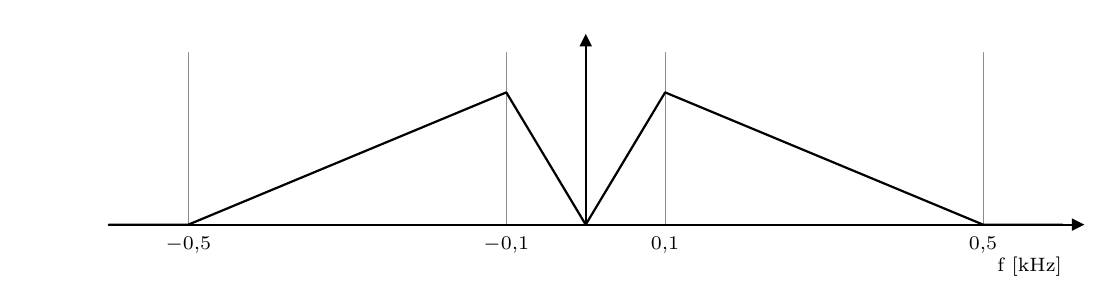
\begin{tikzpicture}[x=0.01985cm,y=-0.01985cm,line cap=round,line join=round]
\useasboundingbox (0,0) rectangle (680,160);
\path[draw=black!45,line width=0.35pt] (102.8,126) -- (102.8,16);
\path[draw=black!45,line width=0.35pt] (306.2,126) -- (306.2,16);
\path[draw=black!45,line width=0.35pt] (407.8,126) -- (407.8,16);
\path[draw=black!45,line width=0.35pt] (611.2,126) -- (611.2,16);
\path[draw=black,line width=0.7pt] (52,126) -- (670,126);
\path[fill=black,draw=none] (676,126) -- (668,122) -- (668,130) -- cycle;
\path[draw=black,line width=0.7pt] (357,126) -- (357,10);
\path[fill=black,draw=none] (357,4) -- (353,12) -- (361,12) -- cycle;
\node[anchor=base,inner sep=0pt,font=\scriptsize] at (102.8,142) {$-$0,5};
\node[anchor=base,inner sep=0pt,font=\scriptsize] at (306.2,142) {$-$0,1};
\node[anchor=base,inner sep=0pt,font=\scriptsize] at (407.8,142) {0,1};
\node[anchor=base,inner sep=0pt,font=\scriptsize] at (611.2,142) {0,5};
\node[anchor=base east,inner sep=0pt,font=\scriptsize] at (662,156) {f [kHz]};
\path[draw=black,line width=0.8pt] (52,126) -- (102.8,126) -- (306.2,41.4) -- (357,126) -- (407.8,41.4) -- (611.2,126) -- (662,126);
\end{tikzpicture}\end{center}

\textbf{Az AM/SSB-SC/LSB jel spektruma}\par
\begin{center}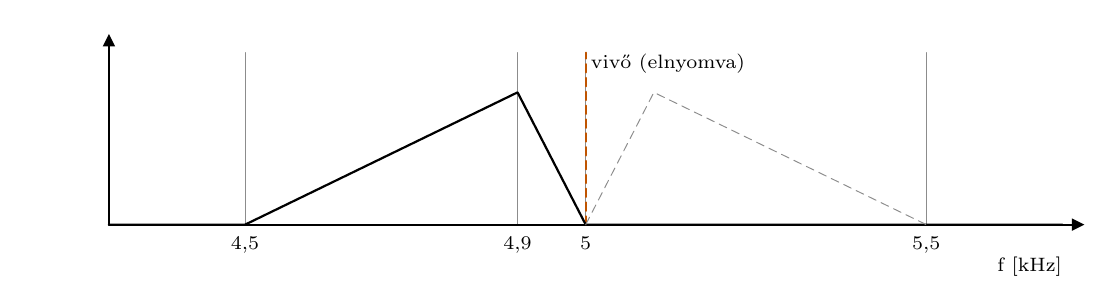
\begin{tikzpicture}[x=0.01985cm,y=-0.01985cm,line cap=round,line join=round]
\useasboundingbox (0,0) rectangle (680,160);
\path[draw=black!45,line width=0.35pt] (139.1,126) -- (139.1,16);
\path[draw=black!45,line width=0.35pt] (313.4,126) -- (313.4,16);
\path[draw=black!45,line width=0.35pt] (357,126) -- (357,16);
\path[draw=black!45,line width=0.35pt] (574.9,126) -- (574.9,16);
\path[draw=black,line width=0.7pt] (52,126) -- (670,126);
\path[fill=black,draw=none] (676,126) -- (668,122) -- (668,130) -- cycle;
\path[draw=black,line width=0.7pt] (52,126) -- (52,10);
\path[fill=black,draw=none] (52,4) -- (48,12) -- (56,12) -- cycle;
\node[anchor=base,inner sep=0pt,font=\scriptsize] at (139.1,142) {4,5};
\node[anchor=base,inner sep=0pt,font=\scriptsize] at (313.4,142) {4,9};
\node[anchor=base,inner sep=0pt,font=\scriptsize] at (357,142) {5};
\node[anchor=base,inner sep=0pt,font=\scriptsize] at (574.9,142) {5,5};
\node[anchor=base east,inner sep=0pt,font=\scriptsize] at (662,156) {f [kHz]};
\path[draw=cB,line width=0.8pt,dash pattern=on 3pt off 2pt] (357,126) -- (357,16);
\node[anchor=base west,inner sep=0pt,font=\scriptsize] at (360,26) {vivő (elnyomva)};
\path[draw=black,line width=0.8pt] (52,126) -- (139.1,126) -- (313.4,41.4) -- (357,126) -- (662,126);
\path[draw=black!45,line width=0.35pt,dash pattern=on 3pt off 2pt] (357,126) -- (400.6,41.4) -- (574.9,126);
\end{tikzpicture}\end{center}
\begin{itemize}
\item Csak az alsó oldalsáv marad: a 0,1\ldots{}0,5 kHz-es rész tükrözve 4,5\ldots{}4,9 kHz-re kerül, a csúcs 4,9 kHz-en. A felső oldalsáv (szürke szaggatott) és a vivő nincs a jelben.
\end{itemize}
\end{rajz}
\begin{eredmeny}

\begin{center}\adjustbox{max width=\linewidth}{$\displaystyle \text{LSB: }4{,}5\ldots5\ \text{kHz, maximum 4,9 kHz-en}\qquad\text{előny: fele sáv, kisebb teljesítmény}\qquad\text{hátrány: koherens vétel}$}\end{center}
\end{eredmeny}

% Generálva: html/build_tex.js (ai06.js). Kézzel ne szerkeszd, a forrás a html/data mappa.
\setcounter{chapter}{5}
\chapter{\texorpdfstring{Digitális alapsávi átvitel (PAM, ISI)}{Digitális alapsávi átvitel (PAM, ISI)}}\label{f6}
Az elemi jelből kell kiolvasni, hogy a mintavételi pillanatban mennyi „lóg át” a szomszéd szimbólumokból, és hogy ez elrontja-e a döntést két-, négy- vagy nyolcszintű jelnél.

\section{Alapok, egyszerűen}
\subsection{\texorpdfstring{A1. Jelölések, ISI és a többszintű jel próbája}{A1. Jelölések, ISI és a többszintű jel próbája}}\label{a6-isi}
\par\noindent{\small\renewcommand{\arraystretch}{1.25}\begin{tabularx}{\linewidth}{@{}>{\raggedright\arraybackslash}X>{\raggedright\arraybackslash}X@{}}\toprule
\textbf{Jel} & \textbf{Jelentés}\\\midrule
undefined & a undefined-adik szimbólum (undefined, illetve undefined)\\
undefined & elemi jel: egyetlen undefined szimbólum válasza a vevőben\\
undefined & az elemi jel a saját mintavételi pillanatában\\
undefined & az elemi jel undefined jelzési idővel arrébb (ez lóg át a szomszéd mintába)\\
undefined & jelzési idő, undefined a szintek száma\\
\bottomrule\end{tabularx}}\par

A minta $x_k=h_0d_k+\sum_{i\ne0}h_id_{k-i}$, a második tag a \textbf{szimbólumközti áthallás (ISI)}. A legrosszabb eset, ha a szomszédok a legnagyobb értékükkel ($M-1$) ellene dolgoznak. A döntési küszöbök a névleges szintek között félúton: $0,\ \pm2h_0,\ \pm4h_0,\ldots$ A szem nyitott, ha

\begin{center}\adjustbox{max width=\linewidth}{$\displaystyle h_0-(M-1)\sum_{i\ne0}|h_i|>0$}\end{center}

és a felső szinteknél a következő küszöböt sem lépi át a minta.

\subsection{\texorpdfstring{A2. Nyquist-feltétel, emelt koszinusz}{A2. Nyquist-feltétel, emelt koszinusz}}\label{a6-nyquist}
ISI-mentes az elemi jel, ha a spektrumát $1/T$-vel eltolva és összegezve frekvenciafüggetlen állandót kapunk. Az emelt koszinusz ilyen: $1/(2T)$-re (ahol az értéke a fele) pontszimmetrikus lecsengéssel, a sáv $(1+\alpha)/(2T)$ alapsávban, $(1+\alpha)/T$ vivőfrekvenciás átvitelnél. Fehér zajra az optimális vevőszűrő az illesztett szűrő: $H_V=\sqrt{H}$, ha az adó és a vevő egyformán osztozik a teljes $H$-n.

% ------------------------------------------------------------------
\section{\texorpdfstring{6.1. feladat: Elemi jel 1,25 és 0,45 (Moodle 2020)}{6.1. feladat: Elemi jel 1,25 és 0,45 (Moodle 2020)}}\label{ai6_01}
\setcounter{lepes}{0}
\begin{feladat}{6.1. feladat}
Bináris PAM, $h(t)=1{,}25$ a $(0,T)$-n, $0{,}45$ a $(T,2T)$-n. b) Van-e ISI, ha a mintavétel fázisa $T_0=3T/4$? c) Alkalmas-e négyszintű rendszerre?

{\footnotesize\sffamily Forrás: ALL-IN 2. oldal $\cdot$ ai2020\_05\_26\_Q2. Címkék: vizsga}
\end{feladat}
\begin{keresunk}
\begin{itemize}
\item b) van-e ISI, és hibázik-e a döntés
\item c) négy szint
\end{itemize}
\end{keresunk}
\begin{jeloles}
\begin{jeltabla}
$\ca{h_0}$ & az elemi jel: 1,25 az első és 0,45 a második jelzési időben & $1{,}25$\\
$\cb{h_1}$ & az elemi jel: 1,25 az első és 0,45 a második jelzési időben & $0{,}45$\\
$T$ & jelzési idő & \\
$h$ & az elemi jel: 1,25 az első és 0,45 a második jelzési időben & \\
$T_0$ & a mintavétel helye a jelzési időn belül & \\
$x_k$ & a k-adik időrésben vett minta & \\
$d_k$ & a k-adik szimbólum (+1 vagy $-$1) & \\
$d_{k-1}$ & az előző szimbólum (+1 vagy $-$1) & \\
$d$ & a szimbólum értéke, +1 az 1-es és $-$1 a 0-s bitre & \\
$x$ & a mintavevő kimenete (egy minta értéke) & \\
\end{jeltabla}
\par\smallskip\textbf{Adott még:}
\begin{itemize}
\item mintavétel az időrés $3T/4$ pontjában
\end{itemize}
\end{jeloles}

\lepes{A minta képlete}
A $3T/4$-es pontban a saját elemi jel első szakasza (1,25) és az előző szimbólum második szakasza (0,45) adódik össze.

\begin{center}\adjustbox{max width=\linewidth}{$\displaystyle x_k={\ca{1{,}25}}\,d_k+{\cb{0{,}45}}\,d_{k-1}$}\end{center}
\jegyzet{definíció}{}

\lepes{b) Kétszintű}
$d=\pm1$, a küszöb 0.

\begin{center}\adjustbox{max width=\linewidth}{$\displaystyle x=\pm({\ca{1{,}25}}\pm{\cb{0{,}45}})=\pm1{,}7\ \text{vagy}\ \pm0{,}8$}\end{center}
\jegyzet{számérték}{a minta függ az előző bittől: van ISI}

\begin{center}\adjustbox{max width=\linewidth}{$\displaystyle 0{,}8>0$}\end{center}
\jegyzet{ellenőrzés}{a döntés így is hibátlan}

\lepes{c) Négyszintű}
$d\in\{\pm1,\pm3\}$, küszöbök $0$ és $\pm2\cdot{\ca{1{,}25}}=\pm2{,}5$, az áthallás legfeljebb $3\cdot{\cb{0{,}45}}=1{,}35$.
\behely{\bh{\ca{h_0}}{\ca{1{,}25}}}

\begin{center}\adjustbox{max width=\linewidth}{$\displaystyle d_k=1:\ {\ca{1{,}25}}-1{,}35=-0{,}1<0$}\end{center}
\jegyzet{behelyettesítés}{átlépi a 0-s küszöböt}
\behely{\bh{\ca{h_0}}{\ca{1{,}25}}}

\begin{center}\adjustbox{max width=\linewidth}{$\displaystyle d_k=1:\ {\ca{1{,}25}}+1{,}35=2{,}6>2{,}5$}\end{center}
\jegyzet{behelyettesítés}{a felső küszöböt is}

\begin{center}\adjustbox{max width=\linewidth}{$\displaystyle d_k=3:\ 3{,}75-1{,}35=2{,}4<2{,}5$}\end{center}
\jegyzet{ellenőrzés}{a 3-as szint is hibázhat}
\begin{eredmeny}

\begin{center}\adjustbox{max width=\linewidth}{$\displaystyle \text{b) van ISI, de a kétszintű döntés hibátlan}\qquad\text{c) négyszintűre nem alkalmas}$}\end{center}
\end{eredmeny}


% ------------------------------------------------------------------
\section{\texorpdfstring{6.2. feladat: Elemi jel 1,05 és 0,15: két-, négy-, nyolcszintű}{6.2. feladat: Elemi jel 1,05 és 0,15: két-, négy-, nyolcszintű}}\label{ai6_02}
\setcounter{lepes}{0}
\begin{feladat}{6.2. feladat}
Bináris PAM, $h=1{,}05$ a $[0,T]$-n, $0{,}15$ a $[T,2T]$-n. Van-e ISI? Milyen mintákat ad a mintavevő? Alkalmas-e négy-, illetve nyolcszintű rendszerre? Illesztett szűrővel ISI-mentessé tehető-e?

{\footnotesize\sffamily Forrás: ALL-IN 116\ldots{}117., 121. oldal $\cdot$ aiD\_6\_2, aiD\_6\_9 (3.4.). Címkék: vizsga}
\end{feladat}
\begin{keresunk}
\begin{itemize}
\item a minták, a négy- és nyolcszintű próba, az illesztett szűrő hatása
\end{itemize}
\end{keresunk}
\begin{jeloles}
\begin{jeltabla}
$\ca{h_0}$ & az elemi jel: 1,05 az első és 0,15 a második jelzési időben & $1{,}05$\\
$\cb{h_1}$ & az elemi jel: 1,05 az első és 0,15 a második jelzési időben & $0{,}15$\\
$h$ & az elemi jel: 1,05 az első és 0,15 a második jelzési időben & \\
$T$ & jelzési idő & \\
$x_k$ & a k-adik időrésben vett minta & \\
$d_k$ & a k-adik szimbólum (+1 vagy $-$1) & \\
$d_{k-1}$ & az előző szimbólum (+1 vagy $-$1) & \\
$d$ & a szimbólum értéke, +1 az 1-es és $-$1 a 0-s bitre & \\
$x$ & a mintavevő kimenete (egy minta értéke) & \\
$M$ & a szintek száma & \\
\end{jeltabla}
\end{jeloles}

\lepes{Kétszintű minták}
$x_k={\ca{1{,}05}}d_k+{\cb{0{,}15}}d_{k-1}$, $d=\pm1$.

\begin{center}\adjustbox{max width=\linewidth}{$\displaystyle x=\pm({\ca{1{,}05}}\pm{\cb{0{,}15}})=\pm0{,}9\ \text{vagy}\ \pm1{,}2$}\end{center}
\jegyzet{számérték}{van ISI, a döntés hibátlan}

\lepes{Négyszintű}
Küszöbök $0$, $\pm2{,}1$, az áthallás legfeljebb $3\cdot{\cb{0{,}15}}=0{,}45$.
\behely{\bh{\ca{h_0}}{\ca{1{,}05}}}

\begin{center}\adjustbox{max width=\linewidth}{$\displaystyle d=1:\ {\ca{1{,}05}}-0{,}45=0{,}6>0\quad\text{és}\quad{\ca{1{,}05}}+0{,}45=1{,}5<2{,}1$}\end{center}
\jegyzet{behelyettesítés}{}

\begin{center}\adjustbox{max width=\linewidth}{$\displaystyle d=3:\ 3{,}15-0{,}45=2{,}7>2{,}1$}\end{center}
\jegyzet{behelyettesítés}{alkalmas}

\lepes{Nyolcszintű}
$d\in\{\pm1,\ldots,\pm7\}$, az áthallás legfeljebb $7\cdot{\cb{0{,}15}}={\ca{1{,}05}}$.
\behely{\bh{\ca{h_0}}{\ca{1{,}05}}}

\begin{center}\adjustbox{max width=\linewidth}{$\displaystyle d=1:\ {\ca{1{,}05}}-{\ca{1{,}05}}=0$}\end{center}
\jegyzet{behelyettesítés}{a szem bezárul, nem alkalmas}

\lepes{Illesztett szűrő}
Az illesztett szűrő a fehér zaj ellen optimális, az ISI-t nem szünteti meg: az elemi jel ettől még két időrésre nyúlik.
\begin{eredmeny}

\begin{center}\adjustbox{max width=\linewidth}{$\displaystyle \pm0{,}9,\ \pm1{,}2\qquad M=4:\ \text{igen}\qquad M=8:\ \text{nem}\qquad\text{illesztett szűrővel nem tehető ISI-mentessé}$}\end{center}
\end{eredmeny}


% ------------------------------------------------------------------
\section{\texorpdfstring{6.3. feladat: $H(f)=h_0T\cos^2(\pi fT/2)$}{6.3. feladat: H(f)=h0Tcos2(pi fT/2)}}\label{ai6_03}
\setcounter{lepes}{0}
\begin{feladat}{6.3. feladat}
Bináris PAM, az elemi jel spektruma $h_0T\cos^2(\tfrac\pi2fT)$, ha $|f|<1/T$. b) Elkerülhető-e az ISI? c) Milyen a fehér zajra optimalizált vevőszűrő? d) Okoz-e ISI-t egy 1200 Hz-es aluláteresztő, ha $T=833$ \textmu{}s?

{\footnotesize\sffamily Forrás: ALL-IN 118\ldots{}119. oldal $\cdot$ aiD\_6\_3 (és 5-ösöm 11. oldal). Címkék: vizsga}
\end{feladat}
\begin{keresunk}
\begin{itemize}
\item b) Nyquist-feltétel
\item c) $H_V$ (a vevőszűrő átvitele)
\item d) ISI az 1200 Hz-es szűrőtől
\end{itemize}
\end{keresunk}
\begin{jeloles}
\begin{jeltabla}
$h_0$ & az elemi jel a saját mintavételi pillanatában & \\
$\ca{T}$ & jelzési idő & $833$\,\textmu{}s\\
$H_V$ & a vevőszűrő átvitele & \emph{keresett}\\
$x$ & tetszőleges szög (az azonosság változója) & \\
$\alpha$ & lekerekítési tényező & \\
\end{jeltabla}
\end{jeloles}

\lepes{Az alak}
$\cos^2x=\tfrac12(1+\cos2x)$:

\begin{center}\adjustbox{max width=\linewidth}{$\displaystyle H(f)=\frac{h_0{\ca{T}}}{2}\left(1+\cos\pi fT\right)$}\end{center}
\jegyzet{átalakítás}{$\alpha=1$-es (100\%-os) emelt koszinusz}

\lepes{b) Nyquist}
A $0\le f\le1/{\ca{T}}$ tartományban a $H(f)$ és a $1/{\ca{T}}$-vel eltolt $H(f-1/{\ca{T}})$ fed át.

\begin{center}\adjustbox{max width=\linewidth}{$\displaystyle \cos^2\!\left(\tfrac\pi2fT-\tfrac\pi2\right)=\sin^2\!\left(\tfrac\pi2fT\right)$}\end{center}
\jegyzet{átalakítás}{}

\begin{center}\adjustbox{max width=\linewidth}{$\displaystyle H(f)+H(f-\tfrac1{\ca{T}})=h_0{\ca{T}}(\cos^2+\sin^2)=h_0{\ca{T}}$}\end{center}
\jegyzet{tétel}{állandó: nincs ISI}

\lepes{c) Vevőszűrő}
Fehér zajnál az illesztett szűrő az optimális: ha az adó- és a vevőszűrő egyformán osztozik a teljes $H(f)$-en, a vevőszűrő $\sqrt{H(f)}$-fel arányos.

\begin{center}\adjustbox{max width=\linewidth}{$\displaystyle H_V(f)=\sqrt{H(f)}\propto\cos\tfrac\pi2fT,\quad|f|<\tfrac1{\ca{T}}$}\end{center}
\jegyzet{definíció}{illesztett szűrő, koszinusz félhullám}

\lepes{d) Az 1200 Hz-es szűrő}
A spektrum $1/{\ca{T}}$-nél ér véget.

\begin{center}\adjustbox{max width=\linewidth}{$\displaystyle \frac1{\ca{T}}=\frac1{833\ \mu\text{s}}=1200\ \text{Hz}$}\end{center}
\jegyzet{számérték}{a szűrő semmit sem vág le}

\begin{rajz}
\textbf{A spektrum és eltolt másolata}\par
\begin{center}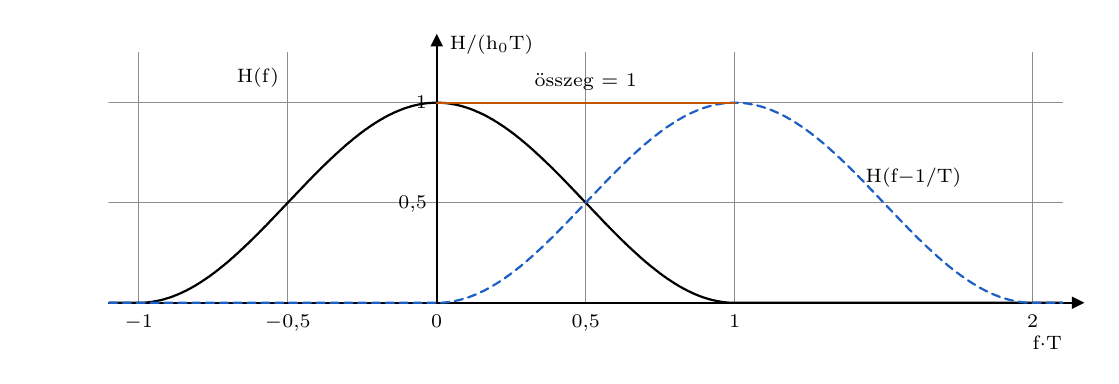
\begin{tikzpicture}[x=0.01985cm,y=-0.01985cm,line cap=round,line join=round]
\useasboundingbox (0,0) rectangle (680,210);
\path[draw=black!45,line width=0.35pt] (71.1,176) -- (71.1,16);
\path[draw=black!45,line width=0.35pt] (166.4,176) -- (166.4,16);
\path[draw=black!45,line width=0.35pt] (261.7,176) -- (261.7,16);
\path[draw=black!45,line width=0.35pt] (357,176) -- (357,16);
\path[draw=black!45,line width=0.35pt] (452.3,176) -- (452.3,16);
\path[draw=black!45,line width=0.35pt] (642.9,176) -- (642.9,16);
\path[draw=black!45,line width=0.35pt] (52,48) -- (662,48);
\path[draw=black!45,line width=0.35pt] (52,112) -- (662,112);
\path[draw=black,line width=0.7pt] (52,176) -- (670,176);
\path[fill=black,draw=none] (676,176) -- (668,172) -- (668,180) -- cycle;
\path[draw=black,line width=0.7pt] (261.7,176) -- (261.7,10);
\path[fill=black,draw=none] (261.7,4) -- (257.7,12) -- (265.7,12) -- cycle;
\node[anchor=base,inner sep=0pt,font=\scriptsize] at (71.1,192) {$-$1};
\node[anchor=base,inner sep=0pt,font=\scriptsize] at (166.4,192) {$-$0,5};
\node[anchor=base,inner sep=0pt,font=\scriptsize] at (261.7,192) {0};
\node[anchor=base,inner sep=0pt,font=\scriptsize] at (357,192) {0,5};
\node[anchor=base,inner sep=0pt,font=\scriptsize] at (452.3,192) {1};
\node[anchor=base,inner sep=0pt,font=\scriptsize] at (642.9,192) {2};
\node[anchor=base east,inner sep=0pt,font=\scriptsize] at (255.7,52) {1};
\node[anchor=base east,inner sep=0pt,font=\scriptsize] at (255.7,116) {0,5};
\node[anchor=base east,inner sep=0pt,font=\scriptsize] at (662,206) {f$\cdot$T};
\node[anchor=base west,inner sep=0pt,font=\scriptsize] at (269.7,14) {H/(h$_0$T)};
\path[draw=black,line width=0.8pt] (52,176) -- (52.8,176) -- (53.5,176) -- (54.3,176) -- (55.1,176) -- (55.8,176) -- (56.6,176) -- (57.3,176) -- (58.1,176) -- (58.9,176) -- (59.6,176) -- (60.4,176) -- (61.2,176) -- (61.9,176) -- (62.7,176) -- (63.4,176) -- (64.2,176) -- (65,176) -- (65.7,176) -- (66.5,176) -- (67.3,176) -- (68,176) -- (68.8,176) -- (69.5,176) -- (70.3,176) -- (71.1,176) -- (71.8,176) -- (72.6,176) -- (73.4,176) -- (74.1,175.9) -- (74.9,175.9) -- (75.6,175.8) -- (76.4,175.8) -- (77.2,175.7) -- (77.9,175.6) -- (78.7,175.5) -- (79.5,175.4) -- (80.2,175.3) -- (81,175.1) -- (81.7,175) -- (82.5,174.9) -- (83.3,174.7) -- (84,174.5) -- (84.8,174.4) -- (85.6,174.2) -- (86.3,174) -- (87.1,173.8) -- (87.8,173.6) -- (88.6,173.3) -- (89.4,173.1) -- (90.1,172.9) -- (90.9,172.6) -- (91.6,172.4) -- (92.4,172.1) -- (93.2,171.8) -- (93.9,171.5) -- (94.7,171.2) -- (95.5,170.9) -- (96.2,170.6) -- (97,170.2) -- (97.8,169.9) -- (98.5,169.6) -- (99.3,169.2) -- (100,168.8) -- (100.8,168.5) -- (101.6,168.1) -- (102.3,167.7) -- (103.1,167.3) -- (103.9,166.9) -- (104.6,166.5) -- (105.4,166) -- (106.1,165.6) -- (106.9,165.2) -- (107.7,164.7) -- (108.4,164.2) -- (109.2,163.8) -- (110,163.3) -- (110.7,162.8) -- (111.5,162.3) -- (112.2,161.8) -- (113,161.3) -- (113.8,160.8) -- (114.5,160.3) -- (115.3,159.7) -- (116.1,159.2) -- (116.8,158.7) -- (117.6,158.1) -- (118.3,157.5) -- (119.1,157) -- (119.9,156.4) -- (120.6,155.8) -- (121.4,155.2) -- (122.2,154.6) -- (122.9,154) -- (123.7,153.4) -- (124.4,152.8) -- (125.2,152.2) -- (126,151.5) -- (126.7,150.9) -- (127.5,150.3) -- (128.3,149.6) -- (129,149) -- (129.8,148.3) -- (130.5,147.6) -- (131.3,147) -- (132.1,146.3) -- (132.8,145.6) -- (133.6,144.9) -- (134.4,144.2) -- (135.1,143.5) -- (135.9,142.8) -- (136.6,142.1) -- (137.4,141.4) -- (138.2,140.7) -- (138.9,140) -- (139.7,139.2) -- (140.5,138.5) -- (141.2,137.8) -- (142,137) -- (142.7,136.3) -- (143.5,135.6) -- (144.3,134.8) -- (145,134.1) -- (145.8,133.3) -- (146.6,132.5) -- (147.3,131.8) -- (148.1,131) -- (148.8,130.2) -- (149.6,129.5) -- (150.4,128.7) -- (151.1,127.9) -- (151.9,127.1) -- (152.7,126.4) -- (153.4,125.6) -- (154.2,124.8) -- (154.9,124) -- (155.7,123.2) -- (156.5,122.4) -- (157.2,121.6) -- (158,120.8) -- (158.8,120) -- (159.5,119.2) -- (160.3,118.4) -- (161,117.6) -- (161.8,116.8) -- (162.6,116) -- (163.3,115.2) -- (164.1,114.4) -- (164.9,113.6) -- (165.6,112.8) -- (166.4,112) -- (167.1,111.2) -- (167.9,110.4) -- (168.7,109.6) -- (169.4,108.8) -- (170.2,108) -- (171,107.2) -- (171.7,106.4) -- (172.5,105.6) -- (173.2,104.8) -- (174,104) -- (174.8,103.2) -- (175.5,102.4) -- (176.3,101.6) -- (177.1,100.8) -- (177.8,100) -- (178.6,99.2) -- (179.3,98.4) -- (180.1,97.6) -- (180.9,96.9) -- (181.6,96.1) -- (182.4,95.3) -- (183.1,94.5) -- (183.9,93.8) -- (184.7,93) -- (185.4,92.2) -- (186.2,91.5) -- (187,90.7) -- (187.7,89.9) -- (188.5,89.2) -- (189.3,88.4) -- (190,87.7) -- (190.8,87) -- (191.5,86.2) -- (192.3,85.5) -- (193.1,84.8) -- (193.8,84) -- (194.6,83.3) -- (195.4,82.6) -- (196.1,81.9) -- (196.9,81.2) -- (197.6,80.5) -- (198.4,79.8) -- (199.2,79.1) -- (199.9,78.4) -- (200.7,77.7) -- (201.5,77) -- (202.2,76.4) -- (203,75.7) -- (203.7,75) -- (204.5,74.4) -- (205.3,73.7) -- (206,73.1) -- (206.8,72.5) -- (207.6,71.8) -- (208.3,71.2) -- (209.1,70.6) -- (209.8,70) -- (210.6,69.4) -- (211.4,68.8) -- (212.1,68.2) -- (212.9,67.6) -- (213.7,67) -- (214.4,66.5) -- (215.2,65.9) -- (215.9,65.3) -- (216.7,64.8) -- (217.5,64.3) -- (218.2,63.7) -- (219,63.2) -- (219.7,62.7) -- (220.5,62.2) -- (221.3,61.7) -- (222,61.2) -- (222.8,60.7) -- (223.6,60.2) -- (224.3,59.8) -- (225.1,59.3) -- (225.9,58.8) -- (226.6,58.4) -- (227.4,58) -- (228.1,57.5) -- (228.9,57.1) -- (229.7,56.7) -- (230.4,56.3) -- (231.2,55.9) -- (232,55.5) -- (232.7,55.2) -- (233.5,54.8) -- (234.2,54.4) -- (235,54.1) -- (235.8,53.8) -- (236.5,53.4) -- (237.3,53.1) -- (238.1,52.8) -- (238.8,52.5) -- (239.6,52.2) -- (240.3,51.9) -- (241.1,51.6) -- (241.9,51.4) -- (242.6,51.1) -- (243.4,50.9) -- (244.2,50.7) -- (244.9,50.4) -- (245.7,50.2) -- (246.4,50) -- (247.2,49.8) -- (248,49.6) -- (248.7,49.5) -- (249.5,49.3) -- (250.3,49.1) -- (251,49) -- (251.8,48.9) -- (252.5,48.7) -- (253.3,48.6) -- (254.1,48.5) -- (254.8,48.4) -- (255.6,48.3) -- (256.4,48.2) -- (257.1,48.2) -- (257.9,48.1) -- (258.6,48.1) -- (259.4,48) -- (260.2,48) -- (260.9,48) -- (261.7,48) -- (262.5,48) -- (263.2,48) -- (264,48) -- (264.7,48.1) -- (265.5,48.1) -- (266.3,48.2) -- (267,48.2) -- (267.8,48.3) -- (268.6,48.4) -- (269.3,48.5) -- (270.1,48.6) -- (270.8,48.7) -- (271.6,48.9) -- (272.4,49) -- (273.1,49.1) -- (273.9,49.3) -- (274.7,49.5) -- (275.4,49.6) -- (276.2,49.8) -- (276.9,50) -- (277.7,50.2) -- (278.5,50.4) -- (279.2,50.7) -- (280,50.9) -- (280.8,51.1) -- (281.5,51.4) -- (282.3,51.6) -- (283,51.9) -- (283.8,52.2) -- (284.6,52.5) -- (285.3,52.8) -- (286.1,53.1) -- (286.8,53.4) -- (287.6,53.8) -- (288.4,54.1) -- (289.1,54.4) -- (289.9,54.8) -- (290.7,55.2) -- (291.4,55.5) -- (292.2,55.9) -- (293,56.3) -- (293.7,56.7) -- (294.5,57.1) -- (295.2,57.5) -- (296,58) -- (296.8,58.4) -- (297.5,58.8) -- (298.3,59.3) -- (299,59.8) -- (299.8,60.2) -- (300.6,60.7) -- (301.3,61.2) -- (302.1,61.7) -- (302.9,62.2) -- (303.6,62.7) -- (304.4,63.2) -- (305.2,63.7) -- (305.9,64.3) -- (306.7,64.8) -- (307.4,65.3) -- (308.2,65.9) -- (309,66.5) -- (309.7,67) -- (310.5,67.6) -- (311.3,68.2) -- (312,68.8) -- (312.8,69.4) -- (313.5,70) -- (314.3,70.6) -- (315.1,71.2) -- (315.8,71.8) -- (316.6,72.5) -- (317.4,73.1) -- (318.1,73.7) -- (318.9,74.4) -- (319.6,75) -- (320.4,75.7) -- (321.2,76.4) -- (321.9,77) -- (322.7,77.7) -- (323.5,78.4) -- (324.2,79.1) -- (325,79.8) -- (325.7,80.5) -- (326.5,81.2) -- (327.3,81.9) -- (328,82.6) -- (328.8,83.3) -- (329.5,84) -- (330.3,84.8) -- (331.1,85.5) -- (331.8,86.2) -- (332.6,87) -- (333.4,87.7) -- (334.1,88.4) -- (334.9,89.2) -- (335.7,89.9) -- (336.4,90.7) -- (337.2,91.5) -- (337.9,92.2) -- (338.7,93) -- (339.5,93.8) -- (340.2,94.5) -- (341,95.3) -- (341.8,96.1) -- (342.5,96.9) -- (343.3,97.6) -- (344,98.4) -- (344.8,99.2) -- (345.6,100) -- (346.3,100.8) -- (347.1,101.6) -- (347.9,102.4) -- (348.6,103.2) -- (349.4,104) -- (350.1,104.8) -- (350.9,105.6) -- (351.7,106.4) -- (352.4,107.2) -- (353.2,108) -- (354,108.8) -- (354.7,109.6) -- (355.5,110.4) -- (356.2,111.2) -- (357,112) -- (357.8,112.8) -- (358.5,113.6) -- (359.3,114.4) -- (360.1,115.2) -- (360.8,116) -- (361.6,116.8) -- (362.3,117.6) -- (363.1,118.4) -- (363.9,119.2) -- (364.6,120) -- (365.4,120.8) -- (366.2,121.6) -- (366.9,122.4) -- (367.7,123.2) -- (368.4,124) -- (369.2,124.8) -- (370,125.6) -- (370.7,126.4) -- (371.5,127.1) -- (372.2,127.9) -- (373,128.7) -- (373.8,129.5) -- (374.5,130.2) -- (375.3,131) -- (376.1,131.8) -- (376.8,132.5) -- (377.6,133.3) -- (378.4,134.1) -- (379.1,134.8) -- (379.9,135.6) -- (380.6,136.3) -- (381.4,137) -- (382.2,137.8) -- (382.9,138.5) -- (383.7,139.2) -- (384.4,140) -- (385.2,140.7) -- (386,141.4) -- (386.7,142.1) -- (387.5,142.8) -- (388.3,143.5) -- (389,144.2) -- (389.8,144.9) -- (390.6,145.6) -- (391.3,146.3) -- (392.1,147) -- (392.8,147.6) -- (393.6,148.3) -- (394.4,149) -- (395.1,149.6) -- (395.9,150.3) -- (396.7,150.9) -- (397.4,151.5) -- (398.2,152.2) -- (398.9,152.8) -- (399.7,153.4) -- (400.5,154) -- (401.2,154.6) -- (402,155.2) -- (402.8,155.8) -- (403.5,156.4) -- (404.3,157) -- (405,157.5) -- (405.8,158.1) -- (406.6,158.7) -- (407.3,159.2) -- (408.1,159.7) -- (408.8,160.3) -- (409.6,160.8) -- (410.4,161.3) -- (411.1,161.8) -- (411.9,162.3) -- (412.7,162.8) -- (413.4,163.3) -- (414.2,163.8) -- (415,164.2) -- (415.7,164.7) -- (416.5,165.2) -- (417.2,165.6) -- (418,166) -- (418.8,166.5) -- (419.5,166.9) -- (420.3,167.3) -- (421.1,167.7) -- (421.8,168.1) -- (422.6,168.5) -- (423.3,168.8) -- (424.1,169.2) -- (424.9,169.6) -- (425.6,169.9) -- (426.4,170.2) -- (427.2,170.6) -- (427.9,170.9) -- (428.7,171.2) -- (429.4,171.5) -- (430.2,171.8) -- (431,172.1) -- (431.7,172.4) -- (432.5,172.6) -- (433.3,172.9) -- (434,173.1) -- (434.8,173.3) -- (435.5,173.6) -- (436.3,173.8) -- (437.1,174) -- (437.8,174.2) -- (438.6,174.4) -- (439.4,174.5) -- (440.1,174.7) -- (440.9,174.9) -- (441.6,175) -- (442.4,175.1) -- (443.2,175.3) -- (443.9,175.4) -- (444.7,175.5) -- (445.5,175.6) -- (446.2,175.7) -- (447,175.8) -- (447.7,175.8) -- (448.5,175.9) -- (449.3,175.9) -- (450,176) -- (450.8,176) -- (451.6,176) -- (452.3,176) -- (453.1,176) -- (453.8,176) -- (454.6,176) -- (455.4,176) -- (456.1,176) -- (456.9,176) -- (457.7,176) -- (458.4,176) -- (459.2,176) -- (459.9,176) -- (460.7,176) -- (461.5,176) -- (462.2,176) -- (463,176) -- (463.8,176) -- (464.5,176) -- (465.3,176) -- (466,176) -- (466.8,176) -- (467.6,176) -- (468.3,176) -- (469.1,176) -- (469.9,176) -- (470.6,176) -- (471.4,176) -- (472.1,176) -- (472.9,176) -- (473.7,176) -- (474.4,176) -- (475.2,176) -- (476,176) -- (476.7,176) -- (477.5,176) -- (478.2,176) -- (479,176) -- (479.8,176) -- (480.5,176) -- (481.3,176) -- (482.1,176) -- (482.8,176) -- (483.6,176) -- (484.3,176) -- (485.1,176) -- (485.9,176) -- (486.6,176) -- (487.4,176) -- (488.2,176) -- (488.9,176) -- (489.7,176) -- (490.4,176) -- (491.2,176) -- (492,176) -- (492.7,176) -- (493.5,176) -- (494.2,176) -- (495,176) -- (495.8,176) -- (496.5,176) -- (497.3,176) -- (498.1,176) -- (498.8,176) -- (499.6,176) -- (500.4,176) -- (501.1,176) -- (501.9,176) -- (502.6,176) -- (503.4,176) -- (504.2,176) -- (504.9,176) -- (505.7,176) -- (506.4,176) -- (507.2,176) -- (508,176) -- (508.7,176) -- (509.5,176) -- (510.3,176) -- (511,176) -- (511.8,176) -- (512.6,176) -- (513.3,176) -- (514.1,176) -- (514.8,176) -- (515.6,176) -- (516.4,176) -- (517.1,176) -- (517.9,176) -- (518.6,176) -- (519.4,176) -- (520.2,176) -- (520.9,176) -- (521.7,176) -- (522.5,176) -- (523.2,176) -- (524,176) -- (524.8,176) -- (525.5,176) -- (526.3,176) -- (527,176) -- (527.8,176) -- (528.6,176) -- (529.3,176) -- (530.1,176) -- (530.8,176) -- (531.6,176) -- (532.4,176) -- (533.1,176) -- (533.9,176) -- (534.7,176) -- (535.4,176) -- (536.2,176) -- (536.9,176) -- (537.7,176) -- (538.5,176) -- (539.2,176) -- (540,176) -- (540.8,176) -- (541.5,176) -- (542.3,176) -- (543.1,176) -- (543.8,176) -- (544.6,176) -- (545.3,176) -- (546.1,176) -- (546.9,176) -- (547.6,176) -- (548.4,176) -- (549.2,176) -- (549.9,176) -- (550.7,176) -- (551.4,176) -- (552.2,176) -- (553,176) -- (553.7,176) -- (554.5,176) -- (555.3,176) -- (556,176) -- (556.8,176) -- (557.5,176) -- (558.3,176) -- (559.1,176) -- (559.8,176) -- (560.6,176) -- (561.3,176) -- (562.1,176) -- (562.9,176) -- (563.6,176) -- (564.4,176) -- (565.2,176) -- (565.9,176) -- (566.7,176) -- (567.4,176) -- (568.2,176) -- (569,176) -- (569.7,176) -- (570.5,176) -- (571.3,176) -- (572,176) -- (572.8,176) -- (573.6,176) -- (574.3,176) -- (575.1,176) -- (575.8,176) -- (576.6,176) -- (577.4,176) -- (578.1,176) -- (578.9,176) -- (579.7,176) -- (580.4,176) -- (581.2,176) -- (581.9,176) -- (582.7,176) -- (583.5,176) -- (584.2,176) -- (585,176) -- (585.7,176) -- (586.5,176) -- (587.3,176) -- (588,176) -- (588.8,176) -- (589.6,176) -- (590.3,176) -- (591.1,176) -- (591.8,176) -- (592.6,176) -- (593.4,176) -- (594.1,176) -- (594.9,176) -- (595.7,176) -- (596.4,176) -- (597.2,176) -- (598,176) -- (598.7,176) -- (599.5,176) -- (600.2,176) -- (601,176) -- (601.8,176) -- (602.5,176) -- (603.3,176) -- (604.1,176) -- (604.8,176) -- (605.6,176) -- (606.3,176) -- (607.1,176) -- (607.9,176) -- (608.6,176) -- (609.4,176) -- (610.2,176) -- (610.9,176) -- (611.7,176) -- (612.4,176) -- (613.2,176) -- (614,176) -- (614.7,176) -- (615.5,176) -- (616.3,176) -- (617,176) -- (617.8,176) -- (618.5,176) -- (619.3,176) -- (620.1,176) -- (620.8,176) -- (621.6,176) -- (622.3,176) -- (623.1,176) -- (623.9,176) -- (624.6,176) -- (625.4,176) -- (626.2,176) -- (626.9,176) -- (627.7,176) -- (628.5,176) -- (629.2,176) -- (630,176) -- (630.7,176) -- (631.5,176) -- (632.3,176) -- (633,176) -- (633.8,176) -- (634.6,176) -- (635.3,176) -- (636.1,176) -- (636.8,176) -- (637.6,176) -- (638.4,176) -- (639.1,176) -- (639.9,176) -- (640.7,176) -- (641.4,176) -- (642.2,176) -- (642.9,176) -- (643.7,176) -- (644.5,176) -- (645.2,176) -- (646,176) -- (646.8,176) -- (647.5,176) -- (648.3,176) -- (649,176) -- (649.8,176) -- (650.6,176) -- (651.3,176) -- (652.1,176) -- (652.9,176) -- (653.6,176) -- (654.4,176) -- (655.1,176) -- (655.9,176) -- (656.7,176) -- (657.4,176) -- (658.2,176) -- (659,176) -- (659.7,176) -- (660.5,176) -- (661.2,176) -- (662,176);
\path[draw=cA,line width=0.8pt,dash pattern=on 3pt off 2pt] (52,176) -- (52.8,176) -- (53.5,176) -- (54.3,176) -- (55.1,176) -- (55.8,176) -- (56.6,176) -- (57.3,176) -- (58.1,176) -- (58.9,176) -- (59.6,176) -- (60.4,176) -- (61.2,176) -- (61.9,176) -- (62.7,176) -- (63.4,176) -- (64.2,176) -- (65,176) -- (65.7,176) -- (66.5,176) -- (67.3,176) -- (68,176) -- (68.8,176) -- (69.5,176) -- (70.3,176) -- (71.1,176) -- (71.8,176) -- (72.6,176) -- (73.4,176) -- (74.1,176) -- (74.9,176) -- (75.6,176) -- (76.4,176) -- (77.2,176) -- (77.9,176) -- (78.7,176) -- (79.5,176) -- (80.2,176) -- (81,176) -- (81.7,176) -- (82.5,176) -- (83.3,176) -- (84,176) -- (84.8,176) -- (85.6,176) -- (86.3,176) -- (87.1,176) -- (87.8,176) -- (88.6,176) -- (89.4,176) -- (90.1,176) -- (90.9,176) -- (91.6,176) -- (92.4,176) -- (93.2,176) -- (93.9,176) -- (94.7,176) -- (95.5,176) -- (96.2,176) -- (97,176) -- (97.8,176) -- (98.5,176) -- (99.3,176) -- (100,176) -- (100.8,176) -- (101.6,176) -- (102.3,176) -- (103.1,176) -- (103.9,176) -- (104.6,176) -- (105.4,176) -- (106.1,176) -- (106.9,176) -- (107.7,176) -- (108.4,176) -- (109.2,176) -- (110,176) -- (110.7,176) -- (111.5,176) -- (112.2,176) -- (113,176) -- (113.8,176) -- (114.5,176) -- (115.3,176) -- (116.1,176) -- (116.8,176) -- (117.6,176) -- (118.3,176) -- (119.1,176) -- (119.9,176) -- (120.6,176) -- (121.4,176) -- (122.2,176) -- (122.9,176) -- (123.7,176) -- (124.4,176) -- (125.2,176) -- (126,176) -- (126.7,176) -- (127.5,176) -- (128.3,176) -- (129,176) -- (129.8,176) -- (130.5,176) -- (131.3,176) -- (132.1,176) -- (132.8,176) -- (133.6,176) -- (134.4,176) -- (135.1,176) -- (135.9,176) -- (136.6,176) -- (137.4,176) -- (138.2,176) -- (138.9,176) -- (139.7,176) -- (140.5,176) -- (141.2,176) -- (142,176) -- (142.7,176) -- (143.5,176) -- (144.3,176) -- (145,176) -- (145.8,176) -- (146.6,176) -- (147.3,176) -- (148.1,176) -- (148.8,176) -- (149.6,176) -- (150.4,176) -- (151.1,176) -- (151.9,176) -- (152.7,176) -- (153.4,176) -- (154.2,176) -- (154.9,176) -- (155.7,176) -- (156.5,176) -- (157.2,176) -- (158,176) -- (158.8,176) -- (159.5,176) -- (160.3,176) -- (161,176) -- (161.8,176) -- (162.6,176) -- (163.3,176) -- (164.1,176) -- (164.9,176) -- (165.6,176) -- (166.4,176) -- (167.1,176) -- (167.9,176) -- (168.7,176) -- (169.4,176) -- (170.2,176) -- (171,176) -- (171.7,176) -- (172.5,176) -- (173.2,176) -- (174,176) -- (174.8,176) -- (175.5,176) -- (176.3,176) -- (177.1,176) -- (177.8,176) -- (178.6,176) -- (179.3,176) -- (180.1,176) -- (180.9,176) -- (181.6,176) -- (182.4,176) -- (183.1,176) -- (183.9,176) -- (184.7,176) -- (185.4,176) -- (186.2,176) -- (187,176) -- (187.7,176) -- (188.5,176) -- (189.3,176) -- (190,176) -- (190.8,176) -- (191.5,176) -- (192.3,176) -- (193.1,176) -- (193.8,176) -- (194.6,176) -- (195.4,176) -- (196.1,176) -- (196.9,176) -- (197.6,176) -- (198.4,176) -- (199.2,176) -- (199.9,176) -- (200.7,176) -- (201.5,176) -- (202.2,176) -- (203,176) -- (203.7,176) -- (204.5,176) -- (205.3,176) -- (206,176) -- (206.8,176) -- (207.6,176) -- (208.3,176) -- (209.1,176) -- (209.8,176) -- (210.6,176) -- (211.4,176) -- (212.1,176) -- (212.9,176) -- (213.7,176) -- (214.4,176) -- (215.2,176) -- (215.9,176) -- (216.7,176) -- (217.5,176) -- (218.2,176) -- (219,176) -- (219.7,176) -- (220.5,176) -- (221.3,176) -- (222,176) -- (222.8,176) -- (223.6,176) -- (224.3,176) -- (225.1,176) -- (225.9,176) -- (226.6,176) -- (227.4,176) -- (228.1,176) -- (228.9,176) -- (229.7,176) -- (230.4,176) -- (231.2,176) -- (232,176) -- (232.7,176) -- (233.5,176) -- (234.2,176) -- (235,176) -- (235.8,176) -- (236.5,176) -- (237.3,176) -- (238.1,176) -- (238.8,176) -- (239.6,176) -- (240.3,176) -- (241.1,176) -- (241.9,176) -- (242.6,176) -- (243.4,176) -- (244.2,176) -- (244.9,176) -- (245.7,176) -- (246.4,176) -- (247.2,176) -- (248,176) -- (248.7,176) -- (249.5,176) -- (250.3,176) -- (251,176) -- (251.8,176) -- (252.5,176) -- (253.3,176) -- (254.1,176) -- (254.8,176) -- (255.6,176) -- (256.4,176) -- (257.1,176) -- (257.9,176) -- (258.6,176) -- (259.4,176) -- (260.2,176) -- (260.9,176) -- (261.7,176) -- (262.5,176) -- (263.2,176) -- (264,176) -- (264.7,175.9) -- (265.5,175.9) -- (266.3,175.8) -- (267,175.8) -- (267.8,175.7) -- (268.6,175.6) -- (269.3,175.5) -- (270.1,175.4) -- (270.8,175.3) -- (271.6,175.1) -- (272.4,175) -- (273.1,174.9) -- (273.9,174.7) -- (274.7,174.5) -- (275.4,174.4) -- (276.2,174.2) -- (276.9,174) -- (277.7,173.8) -- (278.5,173.6) -- (279.2,173.3) -- (280,173.1) -- (280.8,172.9) -- (281.5,172.6) -- (282.3,172.4) -- (283,172.1) -- (283.8,171.8) -- (284.6,171.5) -- (285.3,171.2) -- (286.1,170.9) -- (286.8,170.6) -- (287.6,170.2) -- (288.4,169.9) -- (289.1,169.6) -- (289.9,169.2) -- (290.7,168.8) -- (291.4,168.5) -- (292.2,168.1) -- (293,167.7) -- (293.7,167.3) -- (294.5,166.9) -- (295.2,166.5) -- (296,166) -- (296.8,165.6) -- (297.5,165.2) -- (298.3,164.7) -- (299,164.2) -- (299.8,163.8) -- (300.6,163.3) -- (301.3,162.8) -- (302.1,162.3) -- (302.9,161.8) -- (303.6,161.3) -- (304.4,160.8) -- (305.2,160.3) -- (305.9,159.7) -- (306.7,159.2) -- (307.4,158.7) -- (308.2,158.1) -- (309,157.5) -- (309.7,157) -- (310.5,156.4) -- (311.3,155.8) -- (312,155.2) -- (312.8,154.6) -- (313.5,154) -- (314.3,153.4) -- (315.1,152.8) -- (315.8,152.2) -- (316.6,151.5) -- (317.4,150.9) -- (318.1,150.3) -- (318.9,149.6) -- (319.6,149) -- (320.4,148.3) -- (321.2,147.6) -- (321.9,147) -- (322.7,146.3) -- (323.5,145.6) -- (324.2,144.9) -- (325,144.2) -- (325.7,143.5) -- (326.5,142.8) -- (327.3,142.1) -- (328,141.4) -- (328.8,140.7) -- (329.5,140) -- (330.3,139.2) -- (331.1,138.5) -- (331.8,137.8) -- (332.6,137) -- (333.4,136.3) -- (334.1,135.6) -- (334.9,134.8) -- (335.7,134.1) -- (336.4,133.3) -- (337.2,132.5) -- (337.9,131.8) -- (338.7,131) -- (339.5,130.2) -- (340.2,129.5) -- (341,128.7) -- (341.8,127.9) -- (342.5,127.1) -- (343.3,126.4) -- (344,125.6) -- (344.8,124.8) -- (345.6,124) -- (346.3,123.2) -- (347.1,122.4) -- (347.9,121.6) -- (348.6,120.8) -- (349.4,120) -- (350.1,119.2) -- (350.9,118.4) -- (351.7,117.6) -- (352.4,116.8) -- (353.2,116) -- (354,115.2) -- (354.7,114.4) -- (355.5,113.6) -- (356.2,112.8) -- (357,112) -- (357.8,111.2) -- (358.5,110.4) -- (359.3,109.6) -- (360.1,108.8) -- (360.8,108) -- (361.6,107.2) -- (362.3,106.4) -- (363.1,105.6) -- (363.9,104.8) -- (364.6,104) -- (365.4,103.2) -- (366.2,102.4) -- (366.9,101.6) -- (367.7,100.8) -- (368.4,100) -- (369.2,99.2) -- (370,98.4) -- (370.7,97.6) -- (371.5,96.9) -- (372.2,96.1) -- (373,95.3) -- (373.8,94.5) -- (374.5,93.8) -- (375.3,93) -- (376.1,92.2) -- (376.8,91.5) -- (377.6,90.7) -- (378.4,89.9) -- (379.1,89.2) -- (379.9,88.4) -- (380.6,87.7) -- (381.4,87) -- (382.2,86.2) -- (382.9,85.5) -- (383.7,84.8) -- (384.4,84) -- (385.2,83.3) -- (386,82.6) -- (386.7,81.9) -- (387.5,81.2) -- (388.3,80.5) -- (389,79.8) -- (389.8,79.1) -- (390.6,78.4) -- (391.3,77.7) -- (392.1,77) -- (392.8,76.4) -- (393.6,75.7) -- (394.4,75) -- (395.1,74.4) -- (395.9,73.7) -- (396.7,73.1) -- (397.4,72.5) -- (398.2,71.8) -- (398.9,71.2) -- (399.7,70.6) -- (400.5,70) -- (401.2,69.4) -- (402,68.8) -- (402.8,68.2) -- (403.5,67.6) -- (404.3,67) -- (405,66.5) -- (405.8,65.9) -- (406.6,65.3) -- (407.3,64.8) -- (408.1,64.3) -- (408.8,63.7) -- (409.6,63.2) -- (410.4,62.7) -- (411.1,62.2) -- (411.9,61.7) -- (412.7,61.2) -- (413.4,60.7) -- (414.2,60.2) -- (415,59.8) -- (415.7,59.3) -- (416.5,58.8) -- (417.2,58.4) -- (418,58) -- (418.8,57.5) -- (419.5,57.1) -- (420.3,56.7) -- (421.1,56.3) -- (421.8,55.9) -- (422.6,55.5) -- (423.3,55.2) -- (424.1,54.8) -- (424.9,54.4) -- (425.6,54.1) -- (426.4,53.8) -- (427.2,53.4) -- (427.9,53.1) -- (428.7,52.8) -- (429.4,52.5) -- (430.2,52.2) -- (431,51.9) -- (431.7,51.6) -- (432.5,51.4) -- (433.3,51.1) -- (434,50.9) -- (434.8,50.7) -- (435.5,50.4) -- (436.3,50.2) -- (437.1,50) -- (437.8,49.8) -- (438.6,49.6) -- (439.4,49.5) -- (440.1,49.3) -- (440.9,49.1) -- (441.6,49) -- (442.4,48.9) -- (443.2,48.7) -- (443.9,48.6) -- (444.7,48.5) -- (445.5,48.4) -- (446.2,48.3) -- (447,48.2) -- (447.7,48.2) -- (448.5,48.1) -- (449.3,48.1) -- (450,48) -- (450.8,48) -- (451.6,48) -- (452.3,48) -- (453.1,48) -- (453.8,48) -- (454.6,48) -- (455.4,48.1) -- (456.1,48.1) -- (456.9,48.2) -- (457.7,48.2) -- (458.4,48.3) -- (459.2,48.4) -- (459.9,48.5) -- (460.7,48.6) -- (461.5,48.7) -- (462.2,48.9) -- (463,49) -- (463.8,49.1) -- (464.5,49.3) -- (465.3,49.5) -- (466,49.6) -- (466.8,49.8) -- (467.6,50) -- (468.3,50.2) -- (469.1,50.4) -- (469.9,50.7) -- (470.6,50.9) -- (471.4,51.1) -- (472.1,51.4) -- (472.9,51.6) -- (473.7,51.9) -- (474.4,52.2) -- (475.2,52.5) -- (476,52.8) -- (476.7,53.1) -- (477.5,53.4) -- (478.2,53.8) -- (479,54.1) -- (479.8,54.4) -- (480.5,54.8) -- (481.3,55.2) -- (482.1,55.5) -- (482.8,55.9) -- (483.6,56.3) -- (484.3,56.7) -- (485.1,57.1) -- (485.9,57.5) -- (486.6,58) -- (487.4,58.4) -- (488.2,58.8) -- (488.9,59.3) -- (489.7,59.8) -- (490.4,60.2) -- (491.2,60.7) -- (492,61.2) -- (492.7,61.7) -- (493.5,62.2) -- (494.2,62.7) -- (495,63.2) -- (495.8,63.7) -- (496.5,64.3) -- (497.3,64.8) -- (498.1,65.3) -- (498.8,65.9) -- (499.6,66.5) -- (500.4,67) -- (501.1,67.6) -- (501.9,68.2) -- (502.6,68.8) -- (503.4,69.4) -- (504.2,70) -- (504.9,70.6) -- (505.7,71.2) -- (506.4,71.8) -- (507.2,72.5) -- (508,73.1) -- (508.7,73.7) -- (509.5,74.4) -- (510.3,75) -- (511,75.7) -- (511.8,76.4) -- (512.6,77) -- (513.3,77.7) -- (514.1,78.4) -- (514.8,79.1) -- (515.6,79.8) -- (516.4,80.5) -- (517.1,81.2) -- (517.9,81.9) -- (518.6,82.6) -- (519.4,83.3) -- (520.2,84) -- (520.9,84.8) -- (521.7,85.5) -- (522.5,86.2) -- (523.2,87) -- (524,87.7) -- (524.8,88.4) -- (525.5,89.2) -- (526.3,89.9) -- (527,90.7) -- (527.8,91.5) -- (528.6,92.2) -- (529.3,93) -- (530.1,93.8) -- (530.8,94.5) -- (531.6,95.3) -- (532.4,96.1) -- (533.1,96.9) -- (533.9,97.6) -- (534.7,98.4) -- (535.4,99.2) -- (536.2,100) -- (536.9,100.8) -- (537.7,101.6) -- (538.5,102.4) -- (539.2,103.2) -- (540,104) -- (540.8,104.8) -- (541.5,105.6) -- (542.3,106.4) -- (543.1,107.2) -- (543.8,108) -- (544.6,108.8) -- (545.3,109.6) -- (546.1,110.4) -- (546.9,111.2) -- (547.6,112) -- (548.4,112.8) -- (549.2,113.6) -- (549.9,114.4) -- (550.7,115.2) -- (551.4,116) -- (552.2,116.8) -- (553,117.6) -- (553.7,118.4) -- (554.5,119.2) -- (555.3,120) -- (556,120.8) -- (556.8,121.6) -- (557.5,122.4) -- (558.3,123.2) -- (559.1,124) -- (559.8,124.8) -- (560.6,125.6) -- (561.3,126.4) -- (562.1,127.1) -- (562.9,127.9) -- (563.6,128.7) -- (564.4,129.5) -- (565.2,130.2) -- (565.9,131) -- (566.7,131.8) -- (567.4,132.5) -- (568.2,133.3) -- (569,134.1) -- (569.7,134.8) -- (570.5,135.6) -- (571.3,136.3) -- (572,137) -- (572.8,137.8) -- (573.6,138.5) -- (574.3,139.2) -- (575.1,140) -- (575.8,140.7) -- (576.6,141.4) -- (577.4,142.1) -- (578.1,142.8) -- (578.9,143.5) -- (579.7,144.2) -- (580.4,144.9) -- (581.2,145.6) -- (581.9,146.3) -- (582.7,147) -- (583.5,147.6) -- (584.2,148.3) -- (585,149) -- (585.7,149.6) -- (586.5,150.3) -- (587.3,150.9) -- (588,151.5) -- (588.8,152.2) -- (589.6,152.8) -- (590.3,153.4) -- (591.1,154) -- (591.8,154.6) -- (592.6,155.2) -- (593.4,155.8) -- (594.1,156.4) -- (594.9,157) -- (595.7,157.5) -- (596.4,158.1) -- (597.2,158.7) -- (598,159.2) -- (598.7,159.7) -- (599.5,160.3) -- (600.2,160.8) -- (601,161.3) -- (601.8,161.8) -- (602.5,162.3) -- (603.3,162.8) -- (604.1,163.3) -- (604.8,163.8) -- (605.6,164.2) -- (606.3,164.7) -- (607.1,165.2) -- (607.9,165.6) -- (608.6,166) -- (609.4,166.5) -- (610.2,166.9) -- (610.9,167.3) -- (611.7,167.7) -- (612.4,168.1) -- (613.2,168.5) -- (614,168.8) -- (614.7,169.2) -- (615.5,169.6) -- (616.3,169.9) -- (617,170.2) -- (617.8,170.6) -- (618.5,170.9) -- (619.3,171.2) -- (620.1,171.5) -- (620.8,171.8) -- (621.6,172.1) -- (622.3,172.4) -- (623.1,172.6) -- (623.9,172.9) -- (624.6,173.1) -- (625.4,173.3) -- (626.2,173.6) -- (626.9,173.8) -- (627.7,174) -- (628.5,174.2) -- (629.2,174.4) -- (630,174.5) -- (630.7,174.7) -- (631.5,174.9) -- (632.3,175) -- (633,175.1) -- (633.8,175.3) -- (634.6,175.4) -- (635.3,175.5) -- (636.1,175.6) -- (636.8,175.7) -- (637.6,175.8) -- (638.4,175.8) -- (639.1,175.9) -- (639.9,175.9) -- (640.7,176) -- (641.4,176) -- (642.2,176) -- (642.9,176) -- (643.7,176) -- (644.5,176) -- (645.2,176) -- (646,176) -- (646.8,176) -- (647.5,176) -- (648.3,176) -- (649,176) -- (649.8,176) -- (650.6,176) -- (651.3,176) -- (652.1,176) -- (652.9,176) -- (653.6,176) -- (654.4,176) -- (655.1,176) -- (655.9,176) -- (656.7,176) -- (657.4,176) -- (658.2,176) -- (659,176) -- (659.7,176) -- (660.5,176) -- (661.2,176) -- (662,176);
\path[draw=cB,line width=0.8pt] (261.7,48) -- (452.3,48);
\node[anchor=base,inner sep=0pt,font=\scriptsize] at (147.3,35.2) {H(f)};
\node[anchor=base,inner sep=0pt,font=\scriptsize] at (566.7,99.2) {H(f$-$1/T)};
\node[anchor=base,inner sep=0pt,font=\scriptsize] at (357,37.8) {összeg = 1};
\end{tikzpicture}\end{center}
\begin{itemize}
\item $-1/T$ és $1/T$ között egy „púp”, a csúcsa $f=0$-ban $h_0T$, a fele $f=\pm1/(2T)$-nél.
\item A $1/T$-vel eltolt példány (szaggatott) éppen kiegészíti: az összeg a teljes sávban állandó. Ez a Nyquist-feltétel rajza.
\end{itemize}
\end{rajz}
\begin{eredmeny}

\begin{center}\adjustbox{max width=\linewidth}{$\displaystyle \text{b) ISI-mentes}\qquad\text{c) }H_V\propto\cos(\pi fT/2)\qquad\text{d) nem okoz ISI-t}$}\end{center}
\end{eredmeny}


% ------------------------------------------------------------------
\section{\texorpdfstring{6.4. feladat: $\cos^2$ elemi jel időzítési hibával}{6.4. feladat: cos2 elemi jel időzítési hibával}}\label{ai6_04}
\setcounter{lepes}{0}
\begin{feladat}{6.4. feladat}
$h(t)=h_0\cos^2\left(\frac\pi2\cdot\frac{t-T}{T}\right)$, ha $t\in(0,2T)$. b) Hogyan válasszuk a mintavételt? c) Milyen minták jönnek $t_k=(1{,}1+k)T$-ben? d), e) Négy- és nyolcszintű rendszer a 0,1T-s hibával?

{\footnotesize\sffamily Forrás: ALL-IN 119\ldots{}120. oldal $\cdot$ aiD\_6\_4. Címkék: vizsga, nehezebb}
\end{feladat}
\begin{keresunk}
\begin{itemize}
\item b) a jó mintavételi pillanat
\item c) a minták
\item d), e) négy- és nyolcszintű próba
\end{itemize}
\end{keresunk}
\begin{jeloles}
\begin{jeltabla}
$T$ & jelzési idő & \\
$h_0$ & az elemi jel a saját mintavételi pillanatában & \\
$t_k$ & a k-adik mintavételi pillanat & \\
$x$ & egy minta értéke & \\
$M$ & a szintek száma & \\
$k$ & az időrés sorszáma & \\
\end{jeltabla}
\par\smallskip\textbf{Adott még:}
\begin{itemize}
\item c) a mintavétel $0{,}1T$-vel késik
\end{itemize}
\end{jeloles}

\lepes{b) Ideális mintavétel}
A saját csúcsánál ($t=T$) mintázunk. Ekkor a szomszéd elemi jelek éppen a végükön ($0$ vagy $2T$) vannak.

\begin{center}\adjustbox{max width=\linewidth}{$\displaystyle h(T)=h_0\qquad h(0)=h(2T)=0$}\end{center}
\jegyzet{ellenőrzés}{ISI-mentes}

\lepes{c) 0,1T késés}
A saját elemi jel $1{,}1T$-ben, a következő (egy jelzési idővel később induló) $0{,}1T$-ben van. Az előző már $2{,}1T$-nél tartana, ott 0.

\begin{center}\adjustbox{max width=\linewidth}{$\displaystyle h(1{,}1T)=h_0\cos^2(0{,}05\pi)=0{,}9755\,h_0$}\end{center}
\jegyzet{behelyettesítés}{}

\begin{center}\adjustbox{max width=\linewidth}{$\displaystyle h(0{,}1T)=h_0\cos^2(-0{,}45\pi)=0{,}0245\,h_0$}\end{center}
\jegyzet{behelyettesítés}{}

\begin{center}\adjustbox{max width=\linewidth}{$\displaystyle x=\pm(0{,}9755\pm0{,}0245)h_0=\pm h_0\ \text{vagy}\ \pm0{,}951\,h_0$}\end{center}
\jegyzet{számérték}{kétszintű}

\lepes{d), e) Többszintű próba}
Az áthallás legfeljebb $(M-1)\cdot0{,}0245h_0$.

\begin{center}\adjustbox{max width=\linewidth}{$\displaystyle M=4:\ 0{,}9755-3\cdot0{,}0245=0{,}902>0$}\end{center}
\jegyzet{behelyettesítés}{}

\begin{center}\adjustbox{max width=\linewidth}{$\displaystyle M=8:\ 0{,}9755-7\cdot0{,}0245=0{,}804>0$}\end{center}
\jegyzet{behelyettesítés}{a szem mindkét esetben nyitva}
\begin{eredmeny}

\begin{center}\adjustbox{max width=\linewidth}{$\displaystyle \text{b) }t=(k+1)T\qquad\text{c) }\pm h_0,\ \pm0{,}951h_0\qquad\text{d), e) négy- és nyolcszintű is működik}$}\end{center}
\end{eredmeny}


% ------------------------------------------------------------------
\section{\texorpdfstring{6.5. feladat: 1200 baudos PAM: válasszuk meg $f_1$-et, $f_2$-t és A-t}{6.5. feladat: 1200 baudos PAM: válasszuk meg f1-et, f2-t és A-t}}\label{ai6_05}
\setcounter{lepes}{0}
\begin{feladat}{6.5. feladat}
1200 baudos PAM. A teljes átviteli függvény emelt koszinusz: 0 Hz-en $A$, $f_2$-nél nulla, $f_1=f_2/2$-nél a fele. Biztosítson ISI-mentességet!

{\footnotesize\sffamily Forrás: ALL-IN 120. oldal $\cdot$ aiD\_6\_5 (hivatalos). Címkék: vizsga}
\end{feladat}
\begin{keresunk}
\begin{itemize}
\item $f_1$: ahol a spektrum a felére csökken, $f_2$: ahol nullára csökken, $A$: a spektrum értéke 0 Hz-en
\end{itemize}
\end{keresunk}
\begin{jeloles}
\begin{jeltabla}
$T$ & jelzési idő & \\
$A$ & a spektrum értéke 0 Hz-en & \\
$f_2$ & ahol a spektrum eléri a nullát & \\
$f_1$ & a lapos rész vége & \\
$\alpha$ & lekerekítési tényező & \\
\end{jeltabla}
\end{jeloles}

\lepes{A feltétel}
Nyquist (A2): a lecsengésnek a $1/(2T)$ pontra kell szimmetrikusnak lennie, és ott kell felvennie a felét. Ez a pont tehát $f_1$.

\begin{center}\adjustbox{max width=\linewidth}{$\displaystyle f_1=\frac{1}{2T}=\frac{1200}{2}=600\ \text{Hz}\qquad f_2=2f_1=1200\ \text{Hz}$}\end{center}
\jegyzet{tétel}{$\alpha=1$}

\begin{center}\adjustbox{max width=\linewidth}{$\displaystyle A\ne0\ \text{tetszőleges}$}\end{center}
\jegyzet{ellenőrzés}{csak a jel nagyságát skálázza}
\begin{eredmeny}

\begin{center}\adjustbox{max width=\linewidth}{$\displaystyle f_1=600\ \text{Hz},\ f_2=1200\ \text{Hz},\ A\ne0\ \text{tetszőleges}$}\end{center}
\end{eredmeny}


% ------------------------------------------------------------------
\section{\texorpdfstring{6.6. feladat: Kétutas OOK és Doppler}{6.6. feladat: Kétutas OOK és Doppler}}\label{ai6_06}
\setcounter{lepes}{0}
\begin{feladat}{6.6. feladat}
Az OOK jel két úton jut a vevőbe: $T$ késleltetés és 3 dB csillapítás, illetve $2T$ és 9 dB. A jelzési idő $T$, a vivő $1/T$, az amplitúdósorozat 2022002. a) Rajzolja fel a vett jelet! b) Hogyan változik a jelzési sebesség, ha a vevő nagy sebességgel az adó felé halad?

{\footnotesize\sffamily Forrás: ALL-IN 115\ldots{}116. oldal $\cdot$ aiD\_6\_1. Címkék: vizsga}
\end{feladat}
\begin{keresunk}
\begin{itemize}
\item a) a vett jel amplitúdói
\item b) Doppler-hatás
\end{itemize}
\end{keresunk}
\begin{jeloles}
\begin{jeltabla}
$T$ & jelzési idő & \\
$a_k$ & a k-adik szimbólum amplitúdója & \\
$u_k$ & a vett jel amplitúdója a k-adik időrésben & \\
$a_{k-1}$ & az eggyel korábbi szimbólum & \\
$a_{k-2}$ & a kettővel korábbi szimbólum & \\
$u$ & a vett jel amplitúdója & \\
$u_4$ & a vett jel amplitúdója a 4. időrésben & \\
$v$ & a vevő sebessége & \\
$c$ & a terjedési sebesség (fénysebesség) & \\
\end{jeltabla}
\par\smallskip\textbf{Adott még:}
\begin{itemize}
\item két út: $T$ késés, 3 dB, illetve $2T$ késés, 9 dB
\item OOK: a vivő amplitúdója a szimbólum (2 vagy 0), egy jelzési idő alatt pont egy vivőperiódus
\item $a_k$: 2, 0, 2, 2, 0, 0, 2
\end{itemize}
\end{jeloles}

\lepes{Csillapítások szorzóként}
Feszültségre $20\lg$:

\begin{center}\adjustbox{max width=\linewidth}{$\displaystyle 10^{-3/20}=0{,}71\qquad10^{-9/20}=0{,}35$}\end{center}
\jegyzet{átalakítás}{arányuk éppen 1/2}

\lepes{A vett amplitúdó}
A késések egész vivőperiódusok ($T$ és $2T$), ezért a két út vivője azonos fázisban érkezik, az amplitúdók összeadódnak.

\begin{center}\adjustbox{max width=\linewidth}{$\displaystyle u_k=0{,}71\,a_{k-1}+0{,}35\,a_{k-2}$}\end{center}
\jegyzet{definíció}{}

\begin{center}\adjustbox{max width=\linewidth}{$\displaystyle u:\ 1{,}42;\ 0{,}71;\ 1{,}42;\ 2{,}13;\ 0{,}71;\ 0;\ 1{,}42;\ 0{,}71$}\end{center}
\jegyzet{számérték}{a 2. időréstől, pl. $u_4=0{,}71\cdot2+0{,}35\cdot2$}

\lepes{b) Doppler}
Ha a vevő $v$ sebességgel közeledik, a jel időben összenyomódik: minden frekvencia, a jelzési sebesség is $(1+v/c)$-szeresére nő.

\begin{center}\adjustbox{max width=\linewidth}{$\displaystyle \frac1{T'}=\frac1T\left(1+\frac vc\right)$}\end{center}
\jegyzet{közelítés}{$v\ll c$}

\begin{rajz}
\textbf{A vett jel (a burkoló szintjei feliratozva)}\par
\begin{center}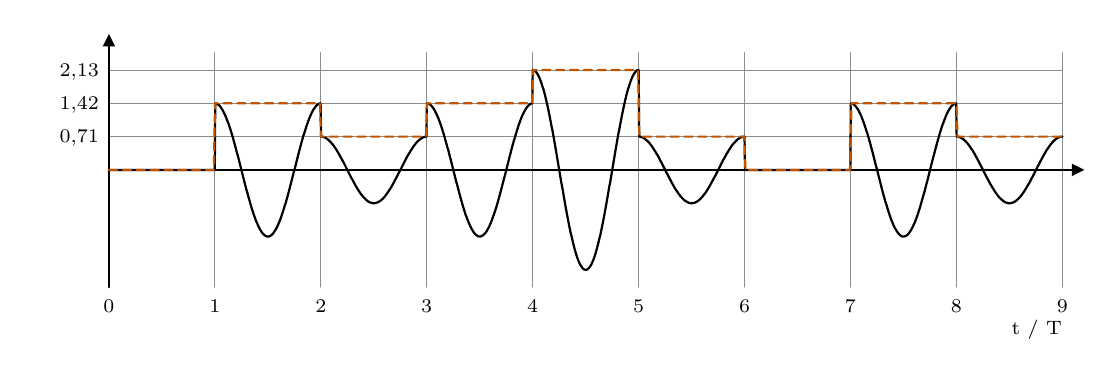
\begin{tikzpicture}[x=0.01985cm,y=-0.01985cm,line cap=round,line join=round]
\useasboundingbox (0,0) rectangle (680,200);
\path[draw=black!45,line width=0.35pt] (52,166) -- (52,16);
\path[draw=black!45,line width=0.35pt] (119.8,166) -- (119.8,16);
\path[draw=black!45,line width=0.35pt] (187.6,166) -- (187.6,16);
\path[draw=black!45,line width=0.35pt] (255.3,166) -- (255.3,16);
\path[draw=black!45,line width=0.35pt] (323.1,166) -- (323.1,16);
\path[draw=black!45,line width=0.35pt] (390.9,166) -- (390.9,16);
\path[draw=black!45,line width=0.35pt] (458.7,166) -- (458.7,16);
\path[draw=black!45,line width=0.35pt] (526.4,166) -- (526.4,16);
\path[draw=black!45,line width=0.35pt] (594.2,166) -- (594.2,16);
\path[draw=black!45,line width=0.35pt] (662,166) -- (662,16);
\path[draw=black!45,line width=0.35pt] (52,27.1) -- (662,27.1);
\path[draw=black!45,line width=0.35pt] (52,48.4) -- (662,48.4);
\path[draw=black!45,line width=0.35pt] (52,69.7) -- (662,69.7);
\path[draw=black,line width=0.7pt] (52,91) -- (670,91);
\path[fill=black,draw=none] (676,91) -- (668,87) -- (668,95) -- cycle;
\path[draw=black,line width=0.7pt] (52,166) -- (52,10);
\path[fill=black,draw=none] (52,4) -- (48,12) -- (56,12) -- cycle;
\node[anchor=base,inner sep=0pt,font=\scriptsize] at (52,182) {0};
\node[anchor=base,inner sep=0pt,font=\scriptsize] at (119.8,182) {1};
\node[anchor=base,inner sep=0pt,font=\scriptsize] at (187.6,182) {2};
\node[anchor=base,inner sep=0pt,font=\scriptsize] at (255.3,182) {3};
\node[anchor=base,inner sep=0pt,font=\scriptsize] at (323.1,182) {4};
\node[anchor=base,inner sep=0pt,font=\scriptsize] at (390.9,182) {5};
\node[anchor=base,inner sep=0pt,font=\scriptsize] at (458.7,182) {6};
\node[anchor=base,inner sep=0pt,font=\scriptsize] at (526.4,182) {7};
\node[anchor=base,inner sep=0pt,font=\scriptsize] at (594.2,182) {8};
\node[anchor=base,inner sep=0pt,font=\scriptsize] at (662,182) {9};
\node[anchor=base east,inner sep=0pt,font=\scriptsize] at (46,31.1) {2,13};
\node[anchor=base east,inner sep=0pt,font=\scriptsize] at (46,52.4) {1,42};
\node[anchor=base east,inner sep=0pt,font=\scriptsize] at (46,73.7) {0,71};
\node[anchor=base east,inner sep=0pt,font=\scriptsize] at (662,196) {t / T};
\path[draw=black,line width=0.8pt] (52,91) -- (52.3,91) -- (52.6,91) -- (52.9,91) -- (53.2,91) -- (53.5,91) -- (53.8,91) -- (54.1,91) -- (54.4,91) -- (54.7,91) -- (55.1,91) -- (55.4,91) -- (55.7,91) -- (56,91) -- (56.3,91) -- (56.6,91) -- (56.9,91) -- (57.2,91) -- (57.5,91) -- (57.8,91) -- (58.1,91) -- (58.4,91) -- (58.7,91) -- (59,91) -- (59.3,91) -- (59.6,91) -- (59.9,91) -- (60.2,91) -- (60.5,91) -- (60.8,91) -- (61.2,91) -- (61.5,91) -- (61.8,91) -- (62.1,91) -- (62.4,91) -- (62.7,91) -- (63,91) -- (63.3,91) -- (63.6,91) -- (63.9,91) -- (64.2,91) -- (64.5,91) -- (64.8,91) -- (65.1,91) -- (65.4,91) -- (65.7,91) -- (66,91) -- (66.3,91) -- (66.6,91) -- (66.9,91) -- (67.3,91) -- (67.6,91) -- (67.9,91) -- (68.2,91) -- (68.5,91) -- (68.8,91) -- (69.1,91) -- (69.4,91) -- (69.7,91) -- (70,91) -- (70.3,91) -- (70.6,91) -- (70.9,91) -- (71.2,91) -- (71.5,91) -- (71.8,91) -- (72.1,91) -- (72.4,91) -- (72.7,91) -- (73,91) -- (73.4,91) -- (73.7,91) -- (74,91) -- (74.3,91) -- (74.6,91) -- (74.9,91) -- (75.2,91) -- (75.5,91) -- (75.8,91) -- (76.1,91) -- (76.4,91) -- (76.7,91) -- (77,91) -- (77.3,91) -- (77.6,91) -- (77.9,91) -- (78.2,91) -- (78.5,91) -- (78.8,91) -- (79.1,91) -- (79.5,91) -- (79.8,91) -- (80.1,91) -- (80.4,91) -- (80.7,91) -- (81,91) -- (81.3,91) -- (81.6,91) -- (81.9,91) -- (82.2,91) -- (82.5,91) -- (82.8,91) -- (83.1,91) -- (83.4,91) -- (83.7,91) -- (84,91) -- (84.3,91) -- (84.6,91) -- (84.9,91) -- (85.2,91) -- (85.6,91) -- (85.9,91) -- (86.2,91) -- (86.5,91) -- (86.8,91) -- (87.1,91) -- (87.4,91) -- (87.7,91) -- (88,91) -- (88.3,91) -- (88.6,91) -- (88.9,91) -- (89.2,91) -- (89.5,91) -- (89.8,91) -- (90.1,91) -- (90.4,91) -- (90.7,91) -- (91,91) -- (91.3,91) -- (91.7,91) -- (92,91) -- (92.3,91) -- (92.6,91) -- (92.9,91) -- (93.2,91) -- (93.5,91) -- (93.8,91) -- (94.1,91) -- (94.4,91) -- (94.7,91) -- (95,91) -- (95.3,91) -- (95.6,91) -- (95.9,91) -- (96.2,91) -- (96.5,91) -- (96.8,91) -- (97.1,91) -- (97.4,91) -- (97.8,91) -- (98.1,91) -- (98.4,91) -- (98.7,91) -- (99,91) -- (99.3,91) -- (99.6,91) -- (99.9,91) -- (100.2,91) -- (100.5,91) -- (100.8,91) -- (101.1,91) -- (101.4,91) -- (101.7,91) -- (102,91) -- (102.3,91) -- (102.6,91) -- (102.9,91) -- (103.2,91) -- (103.5,91) -- (103.9,91) -- (104.2,91) -- (104.5,91) -- (104.8,91) -- (105.1,91) -- (105.4,91) -- (105.7,91) -- (106,91) -- (106.3,91) -- (106.6,91) -- (106.9,91) -- (107.2,91) -- (107.5,91) -- (107.8,91) -- (108.1,91) -- (108.4,91) -- (108.7,91) -- (109,91) -- (109.3,91) -- (109.6,91) -- (110,91) -- (110.3,91) -- (110.6,91) -- (110.9,91) -- (111.2,91) -- (111.5,91) -- (111.8,91) -- (112.1,91) -- (112.4,91) -- (112.7,91) -- (113,91) -- (113.3,91) -- (113.6,91) -- (113.9,91) -- (114.2,91) -- (114.5,91) -- (114.8,91) -- (115.1,91) -- (115.4,91) -- (115.7,91) -- (116.1,91) -- (116.4,91) -- (116.7,91) -- (117,91) -- (117.3,91) -- (117.6,91) -- (117.9,91) -- (118.2,91) -- (118.5,91) -- (118.8,91) -- (119.1,91) -- (119.4,91) -- (119.7,91) -- (120,48.4) -- (120.3,48.5) -- (120.6,48.5) -- (120.9,48.6) -- (121.2,48.8) -- (121.5,49) -- (121.8,49.2) -- (122.2,49.4) -- (122.5,49.7) -- (122.8,50) -- (123.1,50.4) -- (123.4,50.7) -- (123.7,51.2) -- (124,51.6) -- (124.3,52.1) -- (124.6,52.6) -- (124.9,53.1) -- (125.2,53.7) -- (125.5,54.3) -- (125.8,54.9) -- (126.1,55.5) -- (126.4,56.2) -- (126.7,56.9) -- (127,57.7) -- (127.3,58.4) -- (127.6,59.2) -- (127.9,60) -- (128.3,60.9) -- (128.6,61.7) -- (128.9,62.6) -- (129.2,63.5) -- (129.5,64.5) -- (129.8,65.4) -- (130.1,66.4) -- (130.4,67.4) -- (130.7,68.4) -- (131,69.4) -- (131.3,70.5) -- (131.6,71.5) -- (131.9,72.6) -- (132.2,73.7) -- (132.5,74.8) -- (132.8,75.9) -- (133.1,77.1) -- (133.4,78.2) -- (133.7,79.4) -- (134,80.5) -- (134.4,81.7) -- (134.7,82.9) -- (135,84.1) -- (135.3,85.3) -- (135.6,86.5) -- (135.9,87.7) -- (136.2,88.9) -- (136.5,90.1) -- (136.8,91.3) -- (137.1,92.5) -- (137.4,93.7) -- (137.7,94.9) -- (138,96.1) -- (138.3,97.3) -- (138.6,98.5) -- (138.9,99.6) -- (139.2,100.8) -- (139.5,102) -- (139.8,103.1) -- (140.1,104.3) -- (140.5,105.4) -- (140.8,106.6) -- (141.1,107.7) -- (141.4,108.8) -- (141.7,109.9) -- (142,110.9) -- (142.3,112) -- (142.6,113) -- (142.9,114.1) -- (143.2,115.1) -- (143.5,116) -- (143.8,117) -- (144.1,117.9) -- (144.4,118.9) -- (144.7,119.8) -- (145,120.6) -- (145.3,121.5) -- (145.6,122.3) -- (145.9,123.1) -- (146.2,123.9) -- (146.6,124.7) -- (146.9,125.4) -- (147.2,126.1) -- (147.5,126.8) -- (147.8,127.4) -- (148.1,128) -- (148.4,128.6) -- (148.7,129.1) -- (149,129.7) -- (149.3,130.1) -- (149.6,130.6) -- (149.9,131) -- (150.2,131.4) -- (150.5,131.8) -- (150.8,132.1) -- (151.1,132.4) -- (151.4,132.7) -- (151.7,132.9) -- (152,133.1) -- (152.3,133.3) -- (152.7,133.4) -- (153,133.5) -- (153.3,133.6) -- (153.6,133.6) -- (153.9,133.6) -- (154.2,133.6) -- (154.5,133.5) -- (154.8,133.4) -- (155.1,133.2) -- (155.4,133.1) -- (155.7,132.8) -- (156,132.6) -- (156.3,132.3) -- (156.6,132) -- (156.9,131.7) -- (157.2,131.3) -- (157.5,130.9) -- (157.8,130.5) -- (158.1,130) -- (158.4,129.5) -- (158.8,129) -- (159.1,128.4) -- (159.4,127.8) -- (159.7,127.2) -- (160,126.5) -- (160.3,125.9) -- (160.6,125.1) -- (160.9,124.4) -- (161.2,123.7) -- (161.5,122.9) -- (161.8,122.1) -- (162.1,121.2) -- (162.4,120.4) -- (162.7,119.5) -- (163,118.6) -- (163.3,117.6) -- (163.6,116.7) -- (163.9,115.7) -- (164.2,114.7) -- (164.5,113.7) -- (164.9,112.7) -- (165.2,111.6) -- (165.5,110.6) -- (165.8,109.5) -- (166.1,108.4) -- (166.4,107.3) -- (166.7,106.2) -- (167,105.1) -- (167.3,103.9) -- (167.6,102.8) -- (167.9,101.6) -- (168.2,100.4) -- (168.5,99.2) -- (168.8,98.1) -- (169.1,96.9) -- (169.4,95.7) -- (169.7,94.5) -- (170,93.3) -- (170.3,92.1) -- (170.6,90.9) -- (171,89.7) -- (171.3,88.5) -- (171.6,87.3) -- (171.9,86.1) -- (172.2,84.9) -- (172.5,83.7) -- (172.8,82.5) -- (173.1,81.3) -- (173.4,80.1) -- (173.7,79) -- (174,77.8) -- (174.3,76.7) -- (174.6,75.6) -- (174.9,74.5) -- (175.2,73.3) -- (175.5,72.3) -- (175.8,71.2) -- (176.1,70.1) -- (176.4,69.1) -- (176.7,68.1) -- (177.1,67.1) -- (177.4,66.1) -- (177.7,65.1) -- (178,64.2) -- (178.3,63.2) -- (178.6,62.3) -- (178.9,61.5) -- (179.2,60.6) -- (179.5,59.8) -- (179.8,59) -- (180.1,58.2) -- (180.4,57.4) -- (180.7,56.7) -- (181,56) -- (181.3,55.3) -- (181.6,54.7) -- (181.9,54.1) -- (182.2,53.5) -- (182.5,52.9) -- (182.8,52.4) -- (183.2,51.9) -- (183.5,51.4) -- (183.8,51) -- (184.1,50.6) -- (184.4,50.2) -- (184.7,49.9) -- (185,49.6) -- (185.3,49.3) -- (185.6,49.1) -- (185.9,48.9) -- (186.2,48.7) -- (186.5,48.6) -- (186.8,48.5) -- (187.1,48.4) -- (187.4,48.4) -- (187.7,69.7) -- (188,69.7) -- (188.3,69.8) -- (188.6,69.8) -- (188.9,69.9) -- (189.3,70) -- (189.6,70.1) -- (189.9,70.2) -- (190.2,70.3) -- (190.5,70.5) -- (190.8,70.6) -- (191.1,70.8) -- (191.4,71) -- (191.7,71.2) -- (192,71.5) -- (192.3,71.7) -- (192.6,72) -- (192.9,72.3) -- (193.2,72.6) -- (193.5,72.9) -- (193.8,73.2) -- (194.1,73.5) -- (194.4,73.9) -- (194.7,74.3) -- (195,74.6) -- (195.4,75) -- (195.7,75.4) -- (196,75.8) -- (196.3,76.3) -- (196.6,76.7) -- (196.9,77.2) -- (197.2,77.6) -- (197.5,78.1) -- (197.8,78.6) -- (198.1,79.1) -- (198.4,79.6) -- (198.7,80.1) -- (199,80.6) -- (199.3,81.2) -- (199.6,81.7) -- (199.9,82.2) -- (200.2,82.8) -- (200.5,83.3) -- (200.8,83.9) -- (201.1,84.5) -- (201.5,85.1) -- (201.8,85.6) -- (202.1,86.2) -- (202.4,86.8) -- (202.7,87.4) -- (203,88) -- (203.3,88.6) -- (203.6,89.2) -- (203.9,89.8) -- (204.2,90.4) -- (204.5,91) -- (204.8,91.6) -- (205.1,92.2) -- (205.4,92.8) -- (205.7,93.4) -- (206,94) -- (206.3,94.6) -- (206.6,95.2) -- (206.9,95.8) -- (207.2,96.4) -- (207.6,96.9) -- (207.9,97.5) -- (208.2,98.1) -- (208.5,98.7) -- (208.8,99.2) -- (209.1,99.8) -- (209.4,100.3) -- (209.7,100.8) -- (210,101.4) -- (210.3,101.9) -- (210.6,102.4) -- (210.9,102.9) -- (211.2,103.4) -- (211.5,103.9) -- (211.8,104.4) -- (212.1,104.8) -- (212.4,105.3) -- (212.7,105.7) -- (213,106.2) -- (213.3,106.6) -- (213.7,107) -- (214,107.4) -- (214.3,107.7) -- (214.6,108.1) -- (214.9,108.5) -- (215.2,108.8) -- (215.5,109.1) -- (215.8,109.4) -- (216.1,109.7) -- (216.4,110) -- (216.7,110.3) -- (217,110.5) -- (217.3,110.8) -- (217.6,111) -- (217.9,111.2) -- (218.2,111.4) -- (218.5,111.5) -- (218.8,111.7) -- (219.1,111.8) -- (219.4,111.9) -- (219.8,112) -- (220.1,112.1) -- (220.4,112.2) -- (220.7,112.2) -- (221,112.3) -- (221.3,112.3) -- (221.6,112.3) -- (221.9,112.3) -- (222.2,112.2) -- (222.5,112.2) -- (222.8,112.1) -- (223.1,112) -- (223.4,111.9) -- (223.7,111.8) -- (224,111.7) -- (224.3,111.5) -- (224.6,111.4) -- (224.9,111.2) -- (225.2,111) -- (225.5,110.8) -- (225.9,110.5) -- (226.2,110.3) -- (226.5,110) -- (226.8,109.8) -- (227.1,109.5) -- (227.4,109.2) -- (227.7,108.8) -- (228,108.5) -- (228.3,108.2) -- (228.6,107.8) -- (228.9,107.4) -- (229.2,107) -- (229.5,106.6) -- (229.8,106.2) -- (230.1,105.8) -- (230.4,105.3) -- (230.7,104.9) -- (231,104.4) -- (231.3,103.9) -- (231.6,103.5) -- (232,103) -- (232.3,102.5) -- (232.6,102) -- (232.9,101.4) -- (233.2,100.9) -- (233.5,100.4) -- (233.8,99.8) -- (234.1,99.3) -- (234.4,98.7) -- (234.7,98.2) -- (235,97.6) -- (235.3,97) -- (235.6,96.4) -- (235.9,95.8) -- (236.2,95.3) -- (236.5,94.7) -- (236.8,94.1) -- (237.1,93.5) -- (237.4,92.9) -- (237.7,92.3) -- (238.1,91.7) -- (238.4,91.1) -- (238.7,90.5) -- (239,89.9) -- (239.3,89.3) -- (239.6,88.7) -- (239.9,88.1) -- (240.2,87.5) -- (240.5,86.9) -- (240.8,86.3) -- (241.1,85.7) -- (241.4,85.1) -- (241.7,84.5) -- (242,84) -- (242.3,83.4) -- (242.6,82.8) -- (242.9,82.3) -- (243.2,81.7) -- (243.5,81.2) -- (243.8,80.7) -- (244.2,80.2) -- (244.5,79.6) -- (244.8,79.1) -- (245.1,78.6) -- (245.4,78.2) -- (245.7,77.7) -- (246,77.2) -- (246.3,76.8) -- (246.6,76.3) -- (246.9,75.9) -- (247.2,75.5) -- (247.5,75.1) -- (247.8,74.7) -- (248.1,74.3) -- (248.4,73.9) -- (248.7,73.6) -- (249,73.2) -- (249.3,72.9) -- (249.6,72.6) -- (249.9,72.3) -- (250.2,72) -- (250.6,71.8) -- (250.9,71.5) -- (251.2,71.3) -- (251.5,71.1) -- (251.8,70.8) -- (252.1,70.7) -- (252.4,70.5) -- (252.7,70.3) -- (253,70.2) -- (253.3,70.1) -- (253.6,70) -- (253.9,69.9) -- (254.2,69.8) -- (254.5,69.8) -- (254.8,69.7) -- (255.1,69.7) -- (255.4,48.4) -- (255.7,48.4) -- (256,48.5) -- (256.4,48.6) -- (256.7,48.7) -- (257,48.9) -- (257.3,49.1) -- (257.6,49.3) -- (257.9,49.6) -- (258.2,49.9) -- (258.5,50.2) -- (258.8,50.6) -- (259.1,51) -- (259.4,51.4) -- (259.7,51.9) -- (260,52.3) -- (260.3,52.9) -- (260.6,53.4) -- (260.9,54) -- (261.2,54.6) -- (261.5,55.2) -- (261.8,55.9) -- (262.1,56.6) -- (262.5,57.3) -- (262.8,58.1) -- (263.1,58.9) -- (263.4,59.7) -- (263.7,60.5) -- (264,61.4) -- (264.3,62.2) -- (264.6,63.1) -- (264.9,64.1) -- (265.2,65) -- (265.5,66) -- (265.8,66.9) -- (266.1,67.9) -- (266.4,69) -- (266.7,70) -- (267,71.1) -- (267.3,72.1) -- (267.6,73.2) -- (267.9,74.3) -- (268.2,75.4) -- (268.5,76.6) -- (268.9,77.7) -- (269.2,78.9) -- (269.5,80) -- (269.8,81.2) -- (270.1,82.4) -- (270.4,83.5) -- (270.7,84.7) -- (271,85.9) -- (271.3,87.1) -- (271.6,88.3) -- (271.9,89.5) -- (272.2,90.7) -- (272.5,91.9) -- (272.8,93.1) -- (273.1,94.3) -- (273.4,95.5) -- (273.7,96.7) -- (274,97.9) -- (274.3,99.1) -- (274.7,100.3) -- (275,101.5) -- (275.3,102.6) -- (275.6,103.8) -- (275.9,104.9) -- (276.2,106.1) -- (276.5,107.2) -- (276.8,108.3) -- (277.1,109.4) -- (277.4,110.5) -- (277.7,111.5) -- (278,112.6) -- (278.3,113.6) -- (278.6,114.6) -- (278.9,115.6) -- (279.2,116.6) -- (279.5,117.5) -- (279.8,118.5) -- (280.1,119.4) -- (280.4,120.3) -- (280.8,121.1) -- (281.1,122) -- (281.4,122.8) -- (281.7,123.6) -- (282,124.3) -- (282.3,125.1) -- (282.6,125.8) -- (282.9,126.5) -- (283.2,127.1) -- (283.5,127.7) -- (283.8,128.3) -- (284.1,128.9) -- (284.4,129.4) -- (284.7,129.9) -- (285,130.4) -- (285.3,130.8) -- (285.6,131.3) -- (285.9,131.6) -- (286.2,132) -- (286.5,132.3) -- (286.9,132.6) -- (287.2,132.8) -- (287.5,133) -- (287.8,133.2) -- (288.1,133.4) -- (288.4,133.5) -- (288.7,133.5) -- (289,133.6) -- (289.3,133.6) -- (289.6,133.6) -- (289.9,133.5) -- (290.2,133.4) -- (290.5,133.3) -- (290.8,133.1) -- (291.1,132.9) -- (291.4,132.7) -- (291.7,132.5) -- (292,132.2) -- (292.3,131.8) -- (292.6,131.5) -- (293,131.1) -- (293.3,130.7) -- (293.6,130.2) -- (293.9,129.7) -- (294.2,129.2) -- (294.5,128.6) -- (294.8,128.1) -- (295.1,127.5) -- (295.4,126.8) -- (295.7,126.2) -- (296,125.5) -- (296.3,124.7) -- (296.6,124) -- (296.9,123.2) -- (297.2,122.4) -- (297.5,121.6) -- (297.8,120.7) -- (298.1,119.9) -- (298.4,119) -- (298.7,118.1) -- (299.1,117.1) -- (299.4,116.1) -- (299.7,115.2) -- (300,114.2) -- (300.3,113.1) -- (300.6,112.1) -- (300.9,111.1) -- (301.2,110) -- (301.5,108.9) -- (301.8,107.8) -- (302.1,106.7) -- (302.4,105.6) -- (302.7,104.4) -- (303,103.3) -- (303.3,102.1) -- (303.6,100.9) -- (303.9,99.8) -- (304.2,98.6) -- (304.5,97.4) -- (304.8,96.2) -- (305.2,95) -- (305.5,93.8) -- (305.8,92.6) -- (306.1,91.4) -- (306.4,90.2) -- (306.7,89) -- (307,87.8) -- (307.3,86.6) -- (307.6,85.4) -- (307.9,84.2) -- (308.2,83) -- (308.5,81.8) -- (308.8,80.7) -- (309.1,79.5) -- (309.4,78.3) -- (309.7,77.2) -- (310,76.1) -- (310.3,74.9) -- (310.6,73.8) -- (310.9,72.7) -- (311.3,71.7) -- (311.6,70.6) -- (311.9,69.5) -- (312.2,68.5) -- (312.5,67.5) -- (312.8,66.5) -- (313.1,65.5) -- (313.4,64.6) -- (313.7,63.6) -- (314,62.7) -- (314.3,61.8) -- (314.6,61) -- (314.9,60.1) -- (315.2,59.3) -- (315.5,58.5) -- (315.8,57.8) -- (316.1,57) -- (316.4,56.3) -- (316.7,55.6) -- (317,55) -- (317.4,54.3) -- (317.7,53.7) -- (318,53.2) -- (318.3,52.6) -- (318.6,52.1) -- (318.9,51.6) -- (319.2,51.2) -- (319.5,50.8) -- (319.8,50.4) -- (320.1,50.1) -- (320.4,49.7) -- (320.7,49.5) -- (321,49.2) -- (321.3,49) -- (321.6,48.8) -- (321.9,48.7) -- (322.2,48.5) -- (322.5,48.5) -- (322.8,48.4) -- (323.1,27.1) -- (323.5,27.1) -- (323.8,27.2) -- (324.1,27.3) -- (324.4,27.5) -- (324.7,27.8) -- (325,28.1) -- (325.3,28.4) -- (325.6,28.8) -- (325.9,29.2) -- (326.2,29.7) -- (326.5,30.2) -- (326.8,30.8) -- (327.1,31.4) -- (327.4,32.1) -- (327.7,32.8) -- (328,33.6) -- (328.3,34.4) -- (328.6,35.3) -- (328.9,36.2) -- (329.2,37.2) -- (329.5,38.1) -- (329.9,39.2) -- (330.2,40.3) -- (330.5,41.4) -- (330.8,42.5) -- (331.1,43.7) -- (331.4,45) -- (331.7,46.2) -- (332,47.6) -- (332.3,48.9) -- (332.6,50.3) -- (332.9,51.7) -- (333.2,53.1) -- (333.5,54.6) -- (333.8,56.1) -- (334.1,57.6) -- (334.4,59.2) -- (334.7,60.7) -- (335,62.3) -- (335.3,64) -- (335.7,65.6) -- (336,67.3) -- (336.3,69) -- (336.6,70.7) -- (336.9,72.4) -- (337.2,74.1) -- (337.5,75.9) -- (337.8,77.6) -- (338.1,79.4) -- (338.4,81.2) -- (338.7,83) -- (339,84.8) -- (339.3,86.6) -- (339.6,88.4) -- (339.9,90.2) -- (340.2,92) -- (340.5,93.8) -- (340.8,95.6) -- (341.1,97.4) -- (341.4,99.2) -- (341.8,101) -- (342.1,102.8) -- (342.4,104.5) -- (342.7,106.3) -- (343,108.1) -- (343.3,109.8) -- (343.6,111.5) -- (343.9,113.2) -- (344.2,114.9) -- (344.5,116.6) -- (344.8,118.2) -- (345.1,119.8) -- (345.4,121.4) -- (345.7,123) -- (346,124.6) -- (346.3,126.1) -- (346.6,127.6) -- (346.9,129) -- (347.2,130.5) -- (347.5,131.9) -- (347.9,133.3) -- (348.2,134.6) -- (348.5,135.9) -- (348.8,137.2) -- (349.1,138.4) -- (349.4,139.6) -- (349.7,140.7) -- (350,141.9) -- (350.3,142.9) -- (350.6,144) -- (350.9,145) -- (351.2,145.9) -- (351.5,146.8) -- (351.8,147.7) -- (352.1,148.5) -- (352.4,149.2) -- (352.7,150) -- (353,150.6) -- (353.3,151.3) -- (353.6,151.8) -- (354,152.4) -- (354.3,152.8) -- (354.6,153.3) -- (354.9,153.7) -- (355.2,154) -- (355.5,154.3) -- (355.8,154.5) -- (356.1,154.7) -- (356.4,154.8) -- (356.7,154.9) -- (357,154.9) -- (357.3,154.9) -- (357.6,154.8) -- (357.9,154.7) -- (358.2,154.5) -- (358.5,154.3) -- (358.8,154) -- (359.1,153.7) -- (359.4,153.3) -- (359.7,152.8) -- (360.1,152.4) -- (360.4,151.8) -- (360.7,151.3) -- (361,150.6) -- (361.3,150) -- (361.6,149.2) -- (361.9,148.5) -- (362.2,147.7) -- (362.5,146.8) -- (362.8,145.9) -- (363.1,145) -- (363.4,144) -- (363.7,142.9) -- (364,141.9) -- (364.3,140.7) -- (364.6,139.6) -- (364.9,138.4) -- (365.2,137.2) -- (365.5,135.9) -- (365.8,134.6) -- (366.2,133.3) -- (366.5,131.9) -- (366.8,130.5) -- (367.1,129) -- (367.4,127.6) -- (367.7,126.1) -- (368,124.6) -- (368.3,123) -- (368.6,121.4) -- (368.9,119.8) -- (369.2,118.2) -- (369.5,116.6) -- (369.8,114.9) -- (370.1,113.2) -- (370.4,111.5) -- (370.7,109.8) -- (371,108.1) -- (371.3,106.3) -- (371.6,104.5) -- (371.9,102.8) -- (372.2,101) -- (372.6,99.2) -- (372.9,97.4) -- (373.2,95.6) -- (373.5,93.8) -- (373.8,92) -- (374.1,90.2) -- (374.4,88.4) -- (374.7,86.6) -- (375,84.8) -- (375.3,83) -- (375.6,81.2) -- (375.9,79.4) -- (376.2,77.6) -- (376.5,75.9) -- (376.8,74.1) -- (377.1,72.4) -- (377.4,70.7) -- (377.7,69) -- (378,67.3) -- (378.4,65.6) -- (378.7,64) -- (379,62.3) -- (379.3,60.7) -- (379.6,59.2) -- (379.9,57.6) -- (380.2,56.1) -- (380.5,54.6) -- (380.8,53.1) -- (381.1,51.7) -- (381.4,50.3) -- (381.7,48.9) -- (382,47.6) -- (382.3,46.2) -- (382.6,45) -- (382.9,43.7) -- (383.2,42.5) -- (383.5,41.4) -- (383.8,40.3) -- (384.1,39.2) -- (384.5,38.1) -- (384.8,37.2) -- (385.1,36.2) -- (385.4,35.3) -- (385.7,34.4) -- (386,33.6) -- (386.3,32.8) -- (386.6,32.1) -- (386.9,31.4) -- (387.2,30.8) -- (387.5,30.2) -- (387.8,29.7) -- (388.1,29.2) -- (388.4,28.8) -- (388.7,28.4) -- (389,28.1) -- (389.3,27.8) -- (389.6,27.5) -- (389.9,27.3) -- (390.2,27.2) -- (390.6,27.1) -- (390.9,27.1) -- (391.2,69.7) -- (391.5,69.7) -- (391.8,69.8) -- (392.1,69.8) -- (392.4,69.9) -- (392.7,70) -- (393,70.1) -- (393.3,70.2) -- (393.6,70.4) -- (393.9,70.5) -- (394.2,70.7) -- (394.5,70.9) -- (394.8,71.1) -- (395.1,71.3) -- (395.4,71.6) -- (395.7,71.8) -- (396,72.1) -- (396.3,72.4) -- (396.7,72.7) -- (397,73) -- (397.3,73.3) -- (397.6,73.7) -- (397.9,74) -- (398.2,74.4) -- (398.5,74.8) -- (398.8,75.2) -- (399.1,75.6) -- (399.4,76) -- (399.7,76.4) -- (400,76.9) -- (400.3,77.3) -- (400.6,77.8) -- (400.9,78.3) -- (401.2,78.8) -- (401.5,79.2) -- (401.8,79.8) -- (402.1,80.3) -- (402.4,80.8) -- (402.8,81.3) -- (403.1,81.9) -- (403.4,82.4) -- (403.7,83) -- (404,83.5) -- (404.3,84.1) -- (404.6,84.7) -- (404.9,85.3) -- (405.2,85.8) -- (405.5,86.4) -- (405.8,87) -- (406.1,87.6) -- (406.4,88.2) -- (406.7,88.8) -- (407,89.4) -- (407.3,90) -- (407.6,90.6) -- (407.9,91.2) -- (408.2,91.8) -- (408.5,92.4) -- (408.8,93) -- (409.2,93.6) -- (409.5,94.2) -- (409.8,94.8) -- (410.1,95.4) -- (410.4,96) -- (410.7,96.6) -- (411,97.1) -- (411.3,97.7) -- (411.6,98.3) -- (411.9,98.8) -- (412.2,99.4) -- (412.5,99.9) -- (412.8,100.5) -- (413.1,101) -- (413.4,101.6) -- (413.7,102.1) -- (414,102.6) -- (414.3,103.1) -- (414.6,103.6) -- (415,104.1) -- (415.3,104.5) -- (415.6,105) -- (415.9,105.4) -- (416.2,105.9) -- (416.5,106.3) -- (416.8,106.7) -- (417.1,107.1) -- (417.4,107.5) -- (417.7,107.9) -- (418,108.2) -- (418.3,108.6) -- (418.6,108.9) -- (418.9,109.2) -- (419.2,109.5) -- (419.5,109.8) -- (419.8,110.1) -- (420.1,110.4) -- (420.4,110.6) -- (420.7,110.8) -- (421.1,111) -- (421.4,111.2) -- (421.7,111.4) -- (422,111.6) -- (422.3,111.7) -- (422.6,111.9) -- (422.9,112) -- (423.2,112.1) -- (423.5,112.1) -- (423.8,112.2) -- (424.1,112.3) -- (424.4,112.3) -- (424.7,112.3) -- (425,112.3) -- (425.3,112.3) -- (425.6,112.2) -- (425.9,112.2) -- (426.2,112.1) -- (426.5,112) -- (426.8,111.9) -- (427.2,111.8) -- (427.5,111.6) -- (427.8,111.5) -- (428.1,111.3) -- (428.4,111.1) -- (428.7,110.9) -- (429,110.7) -- (429.3,110.5) -- (429.6,110.2) -- (429.9,109.9) -- (430.2,109.7) -- (430.5,109.4) -- (430.8,109.1) -- (431.1,108.7) -- (431.4,108.4) -- (431.7,108) -- (432,107.7) -- (432.3,107.3) -- (432.6,106.9) -- (432.9,106.5) -- (433.3,106.1) -- (433.6,105.6) -- (433.9,105.2) -- (434.2,104.7) -- (434.5,104.3) -- (434.8,103.8) -- (435.1,103.3) -- (435.4,102.8) -- (435.7,102.3) -- (436,101.8) -- (436.3,101.3) -- (436.6,100.7) -- (436.9,100.2) -- (437.2,99.6) -- (437.5,99.1) -- (437.8,98.5) -- (438.1,98) -- (438.4,97.4) -- (438.7,96.8) -- (439,96.2) -- (439.4,95.6) -- (439.7,95.1) -- (440,94.5) -- (440.3,93.9) -- (440.6,93.3) -- (440.9,92.7) -- (441.2,92.1) -- (441.5,91.5) -- (441.8,90.9) -- (442.1,90.3) -- (442.4,89.7) -- (442.7,89.1) -- (443,88.5) -- (443.3,87.9) -- (443.6,87.3) -- (443.9,86.7) -- (444.2,86.1) -- (444.5,85.5) -- (444.8,84.9) -- (445.1,84.4) -- (445.5,83.8) -- (445.8,83.2) -- (446.1,82.7) -- (446.4,82.1) -- (446.7,81.6) -- (447,81) -- (447.3,80.5) -- (447.6,80) -- (447.9,79.5) -- (448.2,79) -- (448.5,78.5) -- (448.8,78) -- (449.1,77.5) -- (449.4,77.1) -- (449.7,76.6) -- (450,76.2) -- (450.3,75.8) -- (450.6,75.3) -- (450.9,74.9) -- (451.2,74.5) -- (451.6,74.2) -- (451.9,73.8) -- (452.2,73.5) -- (452.5,73.1) -- (452.8,72.8) -- (453.1,72.5) -- (453.4,72.2) -- (453.7,71.9) -- (454,71.7) -- (454.3,71.4) -- (454.6,71.2) -- (454.9,71) -- (455.2,70.8) -- (455.5,70.6) -- (455.8,70.4) -- (456.1,70.3) -- (456.4,70.2) -- (456.7,70) -- (457,69.9) -- (457.3,69.9) -- (457.7,69.8) -- (458,69.7) -- (458.3,69.7) -- (458.6,69.7) -- (458.9,91) -- (459.2,91) -- (459.5,91) -- (459.8,91) -- (460.1,91) -- (460.4,91) -- (460.7,91) -- (461,91) -- (461.3,91) -- (461.6,91) -- (461.9,91) -- (462.2,91) -- (462.5,91) -- (462.8,91) -- (463.1,91) -- (463.4,91) -- (463.8,91) -- (464.1,91) -- (464.4,91) -- (464.7,91) -- (465,91) -- (465.3,91) -- (465.6,91) -- (465.9,91) -- (466.2,91) -- (466.5,91) -- (466.8,91) -- (467.1,91) -- (467.4,91) -- (467.7,91) -- (468,91) -- (468.3,91) -- (468.6,91) -- (468.9,91) -- (469.2,91) -- (469.5,91) -- (469.9,91) -- (470.2,91) -- (470.5,91) -- (470.8,91) -- (471.1,91) -- (471.4,91) -- (471.7,91) -- (472,91) -- (472.3,91) -- (472.6,91) -- (472.9,91) -- (473.2,91) -- (473.5,91) -- (473.8,91) -- (474.1,91) -- (474.4,91) -- (474.7,91) -- (475,91) -- (475.3,91) -- (475.6,91) -- (476,91) -- (476.3,91) -- (476.6,91) -- (476.9,91) -- (477.2,91) -- (477.5,91) -- (477.8,91) -- (478.1,91) -- (478.4,91) -- (478.7,91) -- (479,91) -- (479.3,91) -- (479.6,91) -- (479.9,91) -- (480.2,91) -- (480.5,91) -- (480.8,91) -- (481.1,91) -- (481.4,91) -- (481.7,91) -- (482.1,91) -- (482.4,91) -- (482.7,91) -- (483,91) -- (483.3,91) -- (483.6,91) -- (483.9,91) -- (484.2,91) -- (484.5,91) -- (484.8,91) -- (485.1,91) -- (485.4,91) -- (485.7,91) -- (486,91) -- (486.3,91) -- (486.6,91) -- (486.9,91) -- (487.2,91) -- (487.5,91) -- (487.8,91) -- (488.2,91) -- (488.5,91) -- (488.8,91) -- (489.1,91) -- (489.4,91) -- (489.7,91) -- (490,91) -- (490.3,91) -- (490.6,91) -- (490.9,91) -- (491.2,91) -- (491.5,91) -- (491.8,91) -- (492.1,91) -- (492.4,91) -- (492.7,91) -- (493,91) -- (493.3,91) -- (493.6,91) -- (493.9,91) -- (494.3,91) -- (494.6,91) -- (494.9,91) -- (495.2,91) -- (495.5,91) -- (495.8,91) -- (496.1,91) -- (496.4,91) -- (496.7,91) -- (497,91) -- (497.3,91) -- (497.6,91) -- (497.9,91) -- (498.2,91) -- (498.5,91) -- (498.8,91) -- (499.1,91) -- (499.4,91) -- (499.7,91) -- (500,91) -- (500.4,91) -- (500.7,91) -- (501,91) -- (501.3,91) -- (501.6,91) -- (501.9,91) -- (502.2,91) -- (502.5,91) -- (502.8,91) -- (503.1,91) -- (503.4,91) -- (503.7,91) -- (504,91) -- (504.3,91) -- (504.6,91) -- (504.9,91) -- (505.2,91) -- (505.5,91) -- (505.8,91) -- (506.1,91) -- (506.5,91) -- (506.8,91) -- (507.1,91) -- (507.4,91) -- (507.7,91) -- (508,91) -- (508.3,91) -- (508.6,91) -- (508.9,91) -- (509.2,91) -- (509.5,91) -- (509.8,91) -- (510.1,91) -- (510.4,91) -- (510.7,91) -- (511,91) -- (511.3,91) -- (511.6,91) -- (511.9,91) -- (512.2,91) -- (512.6,91) -- (512.9,91) -- (513.2,91) -- (513.5,91) -- (513.8,91) -- (514.1,91) -- (514.4,91) -- (514.7,91) -- (515,91) -- (515.3,91) -- (515.6,91) -- (515.9,91) -- (516.2,91) -- (516.5,91) -- (516.8,91) -- (517.1,91) -- (517.4,91) -- (517.7,91) -- (518,91) -- (518.3,91) -- (518.7,91) -- (519,91) -- (519.3,91) -- (519.6,91) -- (519.9,91) -- (520.2,91) -- (520.5,91) -- (520.8,91) -- (521.1,91) -- (521.4,91) -- (521.7,91) -- (522,91) -- (522.3,91) -- (522.6,91) -- (522.9,91) -- (523.2,91) -- (523.5,91) -- (523.8,91) -- (524.1,91) -- (524.4,91) -- (524.8,91) -- (525.1,91) -- (525.4,91) -- (525.7,91) -- (526,91) -- (526.3,91) -- (526.6,48.4) -- (526.9,48.4) -- (527.2,48.5) -- (527.5,48.6) -- (527.8,48.7) -- (528.1,48.9) -- (528.4,49.1) -- (528.7,49.3) -- (529,49.6) -- (529.3,49.9) -- (529.6,50.2) -- (529.9,50.6) -- (530.2,51) -- (530.5,51.4) -- (530.9,51.9) -- (531.2,52.4) -- (531.5,52.9) -- (531.8,53.5) -- (532.1,54.1) -- (532.4,54.7) -- (532.7,55.3) -- (533,56) -- (533.3,56.7) -- (533.6,57.4) -- (533.9,58.2) -- (534.2,59) -- (534.5,59.8) -- (534.8,60.6) -- (535.1,61.5) -- (535.4,62.3) -- (535.7,63.2) -- (536,64.2) -- (536.3,65.1) -- (536.6,66.1) -- (537,67.1) -- (537.3,68.1) -- (537.6,69.1) -- (537.9,70.1) -- (538.2,71.2) -- (538.5,72.3) -- (538.8,73.3) -- (539.1,74.5) -- (539.4,75.6) -- (539.7,76.7) -- (540,77.8) -- (540.3,79) -- (540.6,80.1) -- (540.9,81.3) -- (541.2,82.5) -- (541.5,83.7) -- (541.8,84.9) -- (542.1,86.1) -- (542.4,87.3) -- (542.7,88.5) -- (543.1,89.7) -- (543.4,90.9) -- (543.7,92.1) -- (544,93.3) -- (544.3,94.5) -- (544.6,95.7) -- (544.9,96.9) -- (545.2,98.1) -- (545.5,99.2) -- (545.8,100.4) -- (546.1,101.6) -- (546.4,102.8) -- (546.7,103.9) -- (547,105.1) -- (547.3,106.2) -- (547.6,107.3) -- (547.9,108.4) -- (548.2,109.5) -- (548.5,110.6) -- (548.8,111.6) -- (549.2,112.7) -- (549.5,113.7) -- (549.8,114.7) -- (550.1,115.7) -- (550.4,116.7) -- (550.7,117.6) -- (551,118.6) -- (551.3,119.5) -- (551.6,120.4) -- (551.9,121.2) -- (552.2,122.1) -- (552.5,122.9) -- (552.8,123.7) -- (553.1,124.4) -- (553.4,125.1) -- (553.7,125.9) -- (554,126.5) -- (554.3,127.2) -- (554.6,127.8) -- (554.9,128.4) -- (555.3,129) -- (555.6,129.5) -- (555.9,130) -- (556.2,130.5) -- (556.5,130.9) -- (556.8,131.3) -- (557.1,131.7) -- (557.4,132) -- (557.7,132.3) -- (558,132.6) -- (558.3,132.8) -- (558.6,133.1) -- (558.9,133.2) -- (559.2,133.4) -- (559.5,133.5) -- (559.8,133.6) -- (560.1,133.6) -- (560.4,133.6) -- (560.7,133.6) -- (561,133.5) -- (561.3,133.4) -- (561.7,133.3) -- (562,133.1) -- (562.3,132.9) -- (562.6,132.7) -- (562.9,132.4) -- (563.2,132.1) -- (563.5,131.8) -- (563.8,131.4) -- (564.1,131) -- (564.4,130.6) -- (564.7,130.1) -- (565,129.7) -- (565.3,129.1) -- (565.6,128.6) -- (565.9,128) -- (566.2,127.4) -- (566.5,126.8) -- (566.8,126.1) -- (567.1,125.4) -- (567.5,124.7) -- (567.8,123.9) -- (568.1,123.1) -- (568.4,122.3) -- (568.7,121.5) -- (569,120.6) -- (569.3,119.8) -- (569.6,118.9) -- (569.9,117.9) -- (570.2,117) -- (570.5,116) -- (570.8,115.1) -- (571.1,114.1) -- (571.4,113) -- (571.7,112) -- (572,110.9) -- (572.3,109.9) -- (572.6,108.8) -- (572.9,107.7) -- (573.2,106.6) -- (573.6,105.4) -- (573.9,104.3) -- (574.2,103.1) -- (574.5,102) -- (574.8,100.8) -- (575.1,99.6) -- (575.4,98.5) -- (575.7,97.3) -- (576,96.1) -- (576.3,94.9) -- (576.6,93.7) -- (576.9,92.5) -- (577.2,91.3) -- (577.5,90.1) -- (577.8,88.9) -- (578.1,87.7) -- (578.4,86.5) -- (578.7,85.3) -- (579,84.1) -- (579.3,82.9) -- (579.7,81.7) -- (580,80.5) -- (580.3,79.4) -- (580.6,78.2) -- (580.9,77.1) -- (581.2,75.9) -- (581.5,74.8) -- (581.8,73.7) -- (582.1,72.6) -- (582.4,71.5) -- (582.7,70.5) -- (583,69.4) -- (583.3,68.4) -- (583.6,67.4) -- (583.9,66.4) -- (584.2,65.4) -- (584.5,64.5) -- (584.8,63.5) -- (585.1,62.6) -- (585.4,61.7) -- (585.8,60.9) -- (586.1,60) -- (586.4,59.2) -- (586.7,58.4) -- (587,57.7) -- (587.3,56.9) -- (587.6,56.2) -- (587.9,55.5) -- (588.2,54.9) -- (588.5,54.3) -- (588.8,53.7) -- (589.1,53.1) -- (589.4,52.6) -- (589.7,52.1) -- (590,51.6) -- (590.3,51.2) -- (590.6,50.7) -- (590.9,50.4) -- (591.2,50) -- (591.5,49.7) -- (591.9,49.4) -- (592.2,49.2) -- (592.5,49) -- (592.8,48.8) -- (593.1,48.6) -- (593.4,48.5) -- (593.7,48.5) -- (594,48.4) -- (594.3,69.7) -- (594.6,69.7) -- (594.9,69.7) -- (595.2,69.8) -- (595.5,69.9) -- (595.8,69.9) -- (596.1,70) -- (596.4,70.1) -- (596.7,70.3) -- (597,70.4) -- (597.3,70.6) -- (597.6,70.8) -- (598,71) -- (598.3,71.2) -- (598.6,71.4) -- (598.9,71.6) -- (599.2,71.9) -- (599.5,72.2) -- (599.8,72.5) -- (600.1,72.8) -- (600.4,73.1) -- (600.7,73.4) -- (601,73.8) -- (601.3,74.1) -- (601.6,74.5) -- (601.9,74.9) -- (602.2,75.3) -- (602.5,75.7) -- (602.8,76.1) -- (603.1,76.6) -- (603.4,77) -- (603.7,77.5) -- (604.1,77.9) -- (604.4,78.4) -- (604.7,78.9) -- (605,79.4) -- (605.3,79.9) -- (605.6,80.4) -- (605.9,81) -- (606.2,81.5) -- (606.5,82.1) -- (606.8,82.6) -- (607.1,83.2) -- (607.4,83.7) -- (607.7,84.3) -- (608,84.9) -- (608.3,85.4) -- (608.6,86) -- (608.9,86.6) -- (609.2,87.2) -- (609.5,87.8) -- (609.8,88.4) -- (610.2,89) -- (610.5,89.6) -- (610.8,90.2) -- (611.1,90.8) -- (611.4,91.4) -- (611.7,92) -- (612,92.6) -- (612.3,93.2) -- (612.6,93.8) -- (612.9,94.4) -- (613.2,95) -- (613.5,95.6) -- (613.8,96.2) -- (614.1,96.7) -- (614.4,97.3) -- (614.7,97.9) -- (615,98.5) -- (615.3,99) -- (615.6,99.6) -- (615.9,100.1) -- (616.3,100.7) -- (616.6,101.2) -- (616.9,101.7) -- (617.2,102.2) -- (617.5,102.8) -- (617.8,103.2) -- (618.1,103.7) -- (618.4,104.2) -- (618.7,104.7) -- (619,105.1) -- (619.3,105.6) -- (619.6,106) -- (619.9,106.4) -- (620.2,106.8) -- (620.5,107.2) -- (620.8,107.6) -- (621.1,108) -- (621.4,108.3) -- (621.7,108.7) -- (622,109) -- (622.3,109.3) -- (622.7,109.6) -- (623,109.9) -- (623.3,110.2) -- (623.6,110.4) -- (623.9,110.7) -- (624.2,110.9) -- (624.5,111.1) -- (624.8,111.3) -- (625.1,111.5) -- (625.4,111.6) -- (625.7,111.8) -- (626,111.9) -- (626.3,112) -- (626.6,112.1) -- (626.9,112.2) -- (627.2,112.2) -- (627.5,112.3) -- (627.8,112.3) -- (628.1,112.3) -- (628.5,112.3) -- (628.8,112.3) -- (629.1,112.2) -- (629.4,112.2) -- (629.7,112.1) -- (630,112) -- (630.3,111.9) -- (630.6,111.7) -- (630.9,111.6) -- (631.2,111.4) -- (631.5,111.3) -- (631.8,111.1) -- (632.1,110.9) -- (632.4,110.6) -- (632.7,110.4) -- (633,110.1) -- (633.3,109.9) -- (633.6,109.6) -- (633.9,109.3) -- (634.2,108.9) -- (634.6,108.6) -- (634.9,108.3) -- (635.2,107.9) -- (635.5,107.5) -- (635.8,107.2) -- (636.1,106.8) -- (636.4,106.3) -- (636.7,105.9) -- (637,105.5) -- (637.3,105) -- (637.6,104.6) -- (637.9,104.1) -- (638.2,103.6) -- (638.5,103.1) -- (638.8,102.6) -- (639.1,102.1) -- (639.4,101.6) -- (639.7,101.1) -- (640,100.6) -- (640.3,100) -- (640.7,99.5) -- (641,98.9) -- (641.3,98.3) -- (641.6,97.8) -- (641.9,97.2) -- (642.2,96.6) -- (642.5,96) -- (642.8,95.5) -- (643.1,94.9) -- (643.4,94.3) -- (643.7,93.7) -- (644,93.1) -- (644.3,92.5) -- (644.6,91.9) -- (644.9,91.3) -- (645.2,90.7) -- (645.5,90.1) -- (645.8,89.5) -- (646.1,88.9) -- (646.4,88.3) -- (646.8,87.7) -- (647.1,87.1) -- (647.4,86.5) -- (647.7,85.9) -- (648,85.3) -- (648.3,84.7) -- (648.6,84.2) -- (648.9,83.6) -- (649.2,83) -- (649.5,82.5) -- (649.8,81.9) -- (650.1,81.4) -- (650.4,80.9) -- (650.7,80.3) -- (651,79.8) -- (651.3,79.3) -- (651.6,78.8) -- (651.9,78.3) -- (652.2,77.8) -- (652.5,77.4) -- (652.9,76.9) -- (653.2,76.5) -- (653.5,76) -- (653.8,75.6) -- (654.1,75.2) -- (654.4,74.8) -- (654.7,74.4) -- (655,74) -- (655.3,73.7) -- (655.6,73.3) -- (655.9,73) -- (656.2,72.7) -- (656.5,72.4) -- (656.8,72.1) -- (657.1,71.8) -- (657.4,71.6) -- (657.7,71.3) -- (658,71.1) -- (658.3,70.9) -- (658.6,70.7) -- (659,70.5) -- (659.3,70.4) -- (659.6,70.2) -- (659.9,70.1) -- (660.2,70) -- (660.5,69.9) -- (660.8,69.8) -- (661.1,69.8) -- (661.4,69.7) -- (661.7,69.7) -- (662,69.7);
\path[draw=cB,line width=0.8pt,dash pattern=on 3pt off 2pt] (52,91) -- (52.8,91) -- (53.5,91) -- (54.3,91) -- (55.1,91) -- (55.8,91) -- (56.6,91) -- (57.3,91) -- (58.1,91) -- (58.9,91) -- (59.6,91) -- (60.4,91) -- (61.2,91) -- (61.9,91) -- (62.7,91) -- (63.4,91) -- (64.2,91) -- (65,91) -- (65.7,91) -- (66.5,91) -- (67.3,91) -- (68,91) -- (68.8,91) -- (69.5,91) -- (70.3,91) -- (71.1,91) -- (71.8,91) -- (72.6,91) -- (73.4,91) -- (74.1,91) -- (74.9,91) -- (75.6,91) -- (76.4,91) -- (77.2,91) -- (77.9,91) -- (78.7,91) -- (79.5,91) -- (80.2,91) -- (81,91) -- (81.7,91) -- (82.5,91) -- (83.3,91) -- (84,91) -- (84.8,91) -- (85.6,91) -- (86.3,91) -- (87.1,91) -- (87.8,91) -- (88.6,91) -- (89.4,91) -- (90.1,91) -- (90.9,91) -- (91.7,91) -- (92.4,91) -- (93.2,91) -- (93.9,91) -- (94.7,91) -- (95.5,91) -- (96.2,91) -- (97,91) -- (97.8,91) -- (98.5,91) -- (99.3,91) -- (100,91) -- (100.8,91) -- (101.6,91) -- (102.3,91) -- (103.1,91) -- (103.9,91) -- (104.6,91) -- (105.4,91) -- (106.1,91) -- (106.9,91) -- (107.7,91) -- (108.4,91) -- (109.2,91) -- (110,91) -- (110.7,91) -- (111.5,91) -- (112.2,91) -- (113,91) -- (113.8,91) -- (114.5,91) -- (115.3,91) -- (116.1,91) -- (116.8,91) -- (117.6,91) -- (118.3,91) -- (119.1,91) -- (119.9,48.4) -- (120.6,48.4) -- (121.4,48.4) -- (122.2,48.4) -- (122.9,48.4) -- (123.7,48.4) -- (124.4,48.4) -- (125.2,48.4) -- (126,48.4) -- (126.7,48.4) -- (127.5,48.4) -- (128.3,48.4) -- (129,48.4) -- (129.8,48.4) -- (130.5,48.4) -- (131.3,48.4) -- (132.1,48.4) -- (132.8,48.4) -- (133.6,48.4) -- (134.4,48.4) -- (135.1,48.4) -- (135.9,48.4) -- (136.6,48.4) -- (137.4,48.4) -- (138.2,48.4) -- (138.9,48.4) -- (139.7,48.4) -- (140.5,48.4) -- (141.2,48.4) -- (142,48.4) -- (142.7,48.4) -- (143.5,48.4) -- (144.3,48.4) -- (145,48.4) -- (145.8,48.4) -- (146.6,48.4) -- (147.3,48.4) -- (148.1,48.4) -- (148.8,48.4) -- (149.6,48.4) -- (150.4,48.4) -- (151.1,48.4) -- (151.9,48.4) -- (152.7,48.4) -- (153.4,48.4) -- (154.2,48.4) -- (154.9,48.4) -- (155.7,48.4) -- (156.5,48.4) -- (157.2,48.4) -- (158,48.4) -- (158.8,48.4) -- (159.5,48.4) -- (160.3,48.4) -- (161,48.4) -- (161.8,48.4) -- (162.6,48.4) -- (163.3,48.4) -- (164.1,48.4) -- (164.9,48.4) -- (165.6,48.4) -- (166.4,48.4) -- (167.1,48.4) -- (167.9,48.4) -- (168.7,48.4) -- (169.4,48.4) -- (170.2,48.4) -- (171,48.4) -- (171.7,48.4) -- (172.5,48.4) -- (173.2,48.4) -- (174,48.4) -- (174.8,48.4) -- (175.5,48.4) -- (176.3,48.4) -- (177.1,48.4) -- (177.8,48.4) -- (178.6,48.4) -- (179.3,48.4) -- (180.1,48.4) -- (180.9,48.4) -- (181.6,48.4) -- (182.4,48.4) -- (183.2,48.4) -- (183.9,48.4) -- (184.7,48.4) -- (185.4,48.4) -- (186.2,48.4) -- (187,48.4) -- (187.7,69.7) -- (188.5,69.7) -- (189.3,69.7) -- (190,69.7) -- (190.8,69.7) -- (191.5,69.7) -- (192.3,69.7) -- (193.1,69.7) -- (193.8,69.7) -- (194.6,69.7) -- (195.4,69.7) -- (196.1,69.7) -- (196.9,69.7) -- (197.6,69.7) -- (198.4,69.7) -- (199.2,69.7) -- (199.9,69.7) -- (200.7,69.7) -- (201.5,69.7) -- (202.2,69.7) -- (203,69.7) -- (203.7,69.7) -- (204.5,69.7) -- (205.3,69.7) -- (206,69.7) -- (206.8,69.7) -- (207.6,69.7) -- (208.3,69.7) -- (209.1,69.7) -- (209.8,69.7) -- (210.6,69.7) -- (211.4,69.7) -- (212.1,69.7) -- (212.9,69.7) -- (213.7,69.7) -- (214.4,69.7) -- (215.2,69.7) -- (215.9,69.7) -- (216.7,69.7) -- (217.5,69.7) -- (218.2,69.7) -- (219,69.7) -- (219.8,69.7) -- (220.5,69.7) -- (221.3,69.7) -- (222,69.7) -- (222.8,69.7) -- (223.6,69.7) -- (224.3,69.7) -- (225.1,69.7) -- (225.9,69.7) -- (226.6,69.7) -- (227.4,69.7) -- (228.1,69.7) -- (228.9,69.7) -- (229.7,69.7) -- (230.4,69.7) -- (231.2,69.7) -- (232,69.7) -- (232.7,69.7) -- (233.5,69.7) -- (234.2,69.7) -- (235,69.7) -- (235.8,69.7) -- (236.5,69.7) -- (237.3,69.7) -- (238.1,69.7) -- (238.8,69.7) -- (239.6,69.7) -- (240.3,69.7) -- (241.1,69.7) -- (241.9,69.7) -- (242.6,69.7) -- (243.4,69.7) -- (244.2,69.7) -- (244.9,69.7) -- (245.7,69.7) -- (246.4,69.7) -- (247.2,69.7) -- (248,69.7) -- (248.7,69.7) -- (249.5,69.7) -- (250.2,69.7) -- (251,69.7) -- (251.8,69.7) -- (252.5,69.7) -- (253.3,69.7) -- (254.1,69.7) -- (254.8,69.7) -- (255.6,48.4) -- (256.4,48.4) -- (257.1,48.4) -- (257.9,48.4) -- (258.6,48.4) -- (259.4,48.4) -- (260.2,48.4) -- (260.9,48.4) -- (261.7,48.4) -- (262.5,48.4) -- (263.2,48.4) -- (264,48.4) -- (264.7,48.4) -- (265.5,48.4) -- (266.3,48.4) -- (267,48.4) -- (267.8,48.4) -- (268.5,48.4) -- (269.3,48.4) -- (270.1,48.4) -- (270.8,48.4) -- (271.6,48.4) -- (272.4,48.4) -- (273.1,48.4) -- (273.9,48.4) -- (274.7,48.4) -- (275.4,48.4) -- (276.2,48.4) -- (276.9,48.4) -- (277.7,48.4) -- (278.5,48.4) -- (279.2,48.4) -- (280,48.4) -- (280.8,48.4) -- (281.5,48.4) -- (282.3,48.4) -- (283,48.4) -- (283.8,48.4) -- (284.6,48.4) -- (285.3,48.4) -- (286.1,48.4) -- (286.9,48.4) -- (287.6,48.4) -- (288.4,48.4) -- (289.1,48.4) -- (289.9,48.4) -- (290.7,48.4) -- (291.4,48.4) -- (292.2,48.4) -- (293,48.4) -- (293.7,48.4) -- (294.5,48.4) -- (295.2,48.4) -- (296,48.4) -- (296.8,48.4) -- (297.5,48.4) -- (298.3,48.4) -- (299.1,48.4) -- (299.8,48.4) -- (300.6,48.4) -- (301.3,48.4) -- (302.1,48.4) -- (302.9,48.4) -- (303.6,48.4) -- (304.4,48.4) -- (305.2,48.4) -- (305.9,48.4) -- (306.7,48.4) -- (307.4,48.4) -- (308.2,48.4) -- (309,48.4) -- (309.7,48.4) -- (310.5,48.4) -- (311.3,48.4) -- (312,48.4) -- (312.8,48.4) -- (313.5,48.4) -- (314.3,48.4) -- (315.1,48.4) -- (315.8,48.4) -- (316.6,48.4) -- (317.4,48.4) -- (318.1,48.4) -- (318.9,48.4) -- (319.6,48.4) -- (320.4,48.4) -- (321.2,48.4) -- (321.9,48.4) -- (322.7,48.4) -- (323.5,27.1) -- (324.2,27.1) -- (325,27.1) -- (325.7,27.1) -- (326.5,27.1) -- (327.3,27.1) -- (328,27.1) -- (328.8,27.1) -- (329.5,27.1) -- (330.3,27.1) -- (331.1,27.1) -- (331.8,27.1) -- (332.6,27.1) -- (333.4,27.1) -- (334.1,27.1) -- (334.9,27.1) -- (335.7,27.1) -- (336.4,27.1) -- (337.2,27.1) -- (337.9,27.1) -- (338.7,27.1) -- (339.5,27.1) -- (340.2,27.1) -- (341,27.1) -- (341.8,27.1) -- (342.5,27.1) -- (343.3,27.1) -- (344,27.1) -- (344.8,27.1) -- (345.6,27.1) -- (346.3,27.1) -- (347.1,27.1) -- (347.9,27.1) -- (348.6,27.1) -- (349.4,27.1) -- (350.1,27.1) -- (350.9,27.1) -- (351.7,27.1) -- (352.4,27.1) -- (353.2,27.1) -- (354,27.1) -- (354.7,27.1) -- (355.5,27.1) -- (356.2,27.1) -- (357,27.1) -- (357.8,27.1) -- (358.5,27.1) -- (359.3,27.1) -- (360.1,27.1) -- (360.8,27.1) -- (361.6,27.1) -- (362.3,27.1) -- (363.1,27.1) -- (363.9,27.1) -- (364.6,27.1) -- (365.4,27.1) -- (366.2,27.1) -- (366.9,27.1) -- (367.7,27.1) -- (368.4,27.1) -- (369.2,27.1) -- (370,27.1) -- (370.7,27.1) -- (371.5,27.1) -- (372.2,27.1) -- (373,27.1) -- (373.8,27.1) -- (374.5,27.1) -- (375.3,27.1) -- (376.1,27.1) -- (376.8,27.1) -- (377.6,27.1) -- (378.4,27.1) -- (379.1,27.1) -- (379.9,27.1) -- (380.6,27.1) -- (381.4,27.1) -- (382.2,27.1) -- (382.9,27.1) -- (383.7,27.1) -- (384.5,27.1) -- (385.2,27.1) -- (386,27.1) -- (386.7,27.1) -- (387.5,27.1) -- (388.3,27.1) -- (389,27.1) -- (389.8,27.1) -- (390.6,27.1) -- (391.3,69.7) -- (392.1,69.7) -- (392.8,69.7) -- (393.6,69.7) -- (394.4,69.7) -- (395.1,69.7) -- (395.9,69.7) -- (396.7,69.7) -- (397.4,69.7) -- (398.2,69.7) -- (398.9,69.7) -- (399.7,69.7) -- (400.5,69.7) -- (401.2,69.7) -- (402,69.7) -- (402.8,69.7) -- (403.5,69.7) -- (404.3,69.7) -- (405,69.7) -- (405.8,69.7) -- (406.6,69.7) -- (407.3,69.7) -- (408.1,69.7) -- (408.8,69.7) -- (409.6,69.7) -- (410.4,69.7) -- (411.1,69.7) -- (411.9,69.7) -- (412.7,69.7) -- (413.4,69.7) -- (414.2,69.7) -- (415,69.7) -- (415.7,69.7) -- (416.5,69.7) -- (417.2,69.7) -- (418,69.7) -- (418.8,69.7) -- (419.5,69.7) -- (420.3,69.7) -- (421.1,69.7) -- (421.8,69.7) -- (422.6,69.7) -- (423.3,69.7) -- (424.1,69.7) -- (424.9,69.7) -- (425.6,69.7) -- (426.4,69.7) -- (427.2,69.7) -- (427.9,69.7) -- (428.7,69.7) -- (429.4,69.7) -- (430.2,69.7) -- (431,69.7) -- (431.7,69.7) -- (432.5,69.7) -- (433.3,69.7) -- (434,69.7) -- (434.8,69.7) -- (435.5,69.7) -- (436.3,69.7) -- (437.1,69.7) -- (437.8,69.7) -- (438.6,69.7) -- (439.4,69.7) -- (440.1,69.7) -- (440.9,69.7) -- (441.6,69.7) -- (442.4,69.7) -- (443.2,69.7) -- (443.9,69.7) -- (444.7,69.7) -- (445.5,69.7) -- (446.2,69.7) -- (447,69.7) -- (447.7,69.7) -- (448.5,69.7) -- (449.3,69.7) -- (450,69.7) -- (450.8,69.7) -- (451.6,69.7) -- (452.3,69.7) -- (453.1,69.7) -- (453.8,69.7) -- (454.6,69.7) -- (455.4,69.7) -- (456.1,69.7) -- (456.9,69.7) -- (457.7,69.7) -- (458.4,69.7) -- (459.2,91) -- (459.9,91) -- (460.7,91) -- (461.5,91) -- (462.2,91) -- (463,91) -- (463.8,91) -- (464.5,91) -- (465.3,91) -- (466,91) -- (466.8,91) -- (467.6,91) -- (468.3,91) -- (469.1,91) -- (469.9,91) -- (470.6,91) -- (471.4,91) -- (472.1,91) -- (472.9,91) -- (473.7,91) -- (474.4,91) -- (475.2,91) -- (476,91) -- (476.7,91) -- (477.5,91) -- (478.2,91) -- (479,91) -- (479.8,91) -- (480.5,91) -- (481.3,91) -- (482.1,91) -- (482.8,91) -- (483.6,91) -- (484.3,91) -- (485.1,91) -- (485.9,91) -- (486.6,91) -- (487.4,91) -- (488.2,91) -- (488.9,91) -- (489.7,91) -- (490.4,91) -- (491.2,91) -- (492,91) -- (492.7,91) -- (493.5,91) -- (494.3,91) -- (495,91) -- (495.8,91) -- (496.5,91) -- (497.3,91) -- (498.1,91) -- (498.8,91) -- (499.6,91) -- (500.4,91) -- (501.1,91) -- (501.9,91) -- (502.6,91) -- (503.4,91) -- (504.2,91) -- (504.9,91) -- (505.7,91) -- (506.5,91) -- (507.2,91) -- (508,91) -- (508.7,91) -- (509.5,91) -- (510.3,91) -- (511,91) -- (511.8,91) -- (512.6,91) -- (513.3,91) -- (514.1,91) -- (514.8,91) -- (515.6,91) -- (516.4,91) -- (517.1,91) -- (517.9,91) -- (518.7,91) -- (519.4,91) -- (520.2,91) -- (520.9,91) -- (521.7,91) -- (522.5,91) -- (523.2,91) -- (524,91) -- (524.8,91) -- (525.5,91) -- (526.3,91) -- (527,48.4) -- (527.8,48.4) -- (528.6,48.4) -- (529.3,48.4) -- (530.1,48.4) -- (530.9,48.4) -- (531.6,48.4) -- (532.4,48.4) -- (533.1,48.4) -- (533.9,48.4) -- (534.7,48.4) -- (535.4,48.4) -- (536.2,48.4) -- (537,48.4) -- (537.7,48.4) -- (538.5,48.4) -- (539.2,48.4) -- (540,48.4) -- (540.8,48.4) -- (541.5,48.4) -- (542.3,48.4) -- (543.1,48.4) -- (543.8,48.4) -- (544.6,48.4) -- (545.3,48.4) -- (546.1,48.4) -- (546.9,48.4) -- (547.6,48.4) -- (548.4,48.4) -- (549.2,48.4) -- (549.9,48.4) -- (550.7,48.4) -- (551.4,48.4) -- (552.2,48.4) -- (553,48.4) -- (553.7,48.4) -- (554.5,48.4) -- (555.3,48.4) -- (556,48.4) -- (556.8,48.4) -- (557.5,48.4) -- (558.3,48.4) -- (559.1,48.4) -- (559.8,48.4) -- (560.6,48.4) -- (561.3,48.4) -- (562.1,48.4) -- (562.9,48.4) -- (563.6,48.4) -- (564.4,48.4) -- (565.2,48.4) -- (565.9,48.4) -- (566.7,48.4) -- (567.5,48.4) -- (568.2,48.4) -- (569,48.4) -- (569.7,48.4) -- (570.5,48.4) -- (571.3,48.4) -- (572,48.4) -- (572.8,48.4) -- (573.6,48.4) -- (574.3,48.4) -- (575.1,48.4) -- (575.8,48.4) -- (576.6,48.4) -- (577.4,48.4) -- (578.1,48.4) -- (578.9,48.4) -- (579.7,48.4) -- (580.4,48.4) -- (581.2,48.4) -- (581.9,48.4) -- (582.7,48.4) -- (583.5,48.4) -- (584.2,48.4) -- (585,48.4) -- (585.8,48.4) -- (586.5,48.4) -- (587.3,48.4) -- (588,48.4) -- (588.8,48.4) -- (589.6,48.4) -- (590.3,48.4) -- (591.1,48.4) -- (591.9,48.4) -- (592.6,48.4) -- (593.4,48.4) -- (594.1,48.4) -- (594.9,69.7) -- (595.7,69.7) -- (596.4,69.7) -- (597.2,69.7) -- (598,69.7) -- (598.7,69.7) -- (599.5,69.7) -- (600.2,69.7) -- (601,69.7) -- (601.8,69.7) -- (602.5,69.7) -- (603.3,69.7) -- (604.1,69.7) -- (604.8,69.7) -- (605.6,69.7) -- (606.3,69.7) -- (607.1,69.7) -- (607.9,69.7) -- (608.6,69.7) -- (609.4,69.7) -- (610.2,69.7) -- (610.9,69.7) -- (611.7,69.7) -- (612.4,69.7) -- (613.2,69.7) -- (614,69.7) -- (614.7,69.7) -- (615.5,69.7) -- (616.3,69.7) -- (617,69.7) -- (617.8,69.7) -- (618.5,69.7) -- (619.3,69.7) -- (620.1,69.7) -- (620.8,69.7) -- (621.6,69.7) -- (622.3,69.7) -- (623.1,69.7) -- (623.9,69.7) -- (624.6,69.7) -- (625.4,69.7) -- (626.2,69.7) -- (626.9,69.7) -- (627.7,69.7) -- (628.5,69.7) -- (629.2,69.7) -- (630,69.7) -- (630.7,69.7) -- (631.5,69.7) -- (632.3,69.7) -- (633,69.7) -- (633.8,69.7) -- (634.6,69.7) -- (635.3,69.7) -- (636.1,69.7) -- (636.8,69.7) -- (637.6,69.7) -- (638.4,69.7) -- (639.1,69.7) -- (639.9,69.7) -- (640.7,69.7) -- (641.4,69.7) -- (642.2,69.7) -- (642.9,69.7) -- (643.7,69.7) -- (644.5,69.7) -- (645.2,69.7) -- (646,69.7) -- (646.8,69.7) -- (647.5,69.7) -- (648.3,69.7) -- (649,69.7) -- (649.8,69.7) -- (650.6,69.7) -- (651.3,69.7) -- (652.1,69.7) -- (652.9,69.7) -- (653.6,69.7) -- (654.4,69.7) -- (655.1,69.7) -- (655.9,69.7) -- (656.7,69.7) -- (657.4,69.7) -- (658.2,69.7) -- (659,69.7) -- (659.7,69.7) -- (660.5,69.7) -- (661.2,69.7) -- (662,69.7);
\end{tikzpicture}\end{center}
\begin{itemize}
\item Időrésenként egy vivőperiódus, az amplitúdó $0{,}71a_{k-1}+0{,}35a_{k-2}$: 1,42, 0,71, 1,42, 2,13, 0,71, 0, 1,42, 0,71 (az első időrés még üres).
\end{itemize}
\end{rajz}
\begin{eredmeny}

\begin{center}\adjustbox{max width=\linewidth}{$\displaystyle \text{a) burkoló }0{,}71a_{k-1}+0{,}35a_{k-2}:\ 1{,}42;\ 0{,}71;\ 1{,}42;\ 2{,}13;\ 0{,}71;\ 0;\ 1{,}42;\ 0{,}71\qquad\text{b) }(1+v/c)\text{-szeres}$}\end{center}
\end{eredmeny}

% Generálva: html/build_tex.js (ai07.js). Kézzel ne szerkeszd, a forrás a html/data mappa.
\setcounter{chapter}{6}
\chapter{\texorpdfstring{Digitális moduláció: FSK, PSK, QAM}{Digitális moduláció: FSK, PSK, QAM}}\label{f7}
FSK-nál a két jelzőfrekvencia, a löket és az MSK-feltétel, PSK és QAM esetén a konstelláció, az átlagteljesítmény és a hibatűrés (erősítés, csillapítás, fázis) a visszatérő kérdések.

\section{Alapok, egyszerűen}
\subsection{\texorpdfstring{A1. Jelölések, FSK és MSK}{A1. Jelölések, FSK és MSK}}\label{a7-fsk}
\par\noindent{\small\renewcommand{\arraystretch}{1.25}\begin{tabularx}{\linewidth}{@{}>{\raggedright\arraybackslash}X>{\raggedright\arraybackslash}X@{}}\toprule
\textbf{Jel} & \textbf{Jelentés}\\\midrule
undefined & jelzési (bit-) idő, undefined a jelzési sebesség\\
undefined & a 0-s és az 1-es bithez tartozó frekvencia (FSK)\\
undefined & vivőfrekvencia, FSK-nál a kettő átlaga, undefined\\
undefined & frekvencialöket, undefined\\
undefined & a konstelláció pontjainak száma, egy szimbólum undefined bit\\
undefined & lekerekítés, a vivőfrekvenciás sáv undefined\\
\bottomrule\end{tabularx}}\par

\textbf{MSK}, ha $f_D=1/(4T)$, azaz a két frekvencia távolsága $1/(2T)$: egy bit alatt a két jel fáziskülönbsége éppen $\pi$-vel nő. Ez a legkisebb távolság, amellyel a két jel még ortogonális, és a fázis folytonos marad. A sávszélességre Carson-jellegű becslés $B\approx2(f_D+f_m)$, ahol a moduláló bitjel alapharmonikusa $f_m=1/(2T)$ \texttt{[ELLENŐRIZENDŐ]} (a tárgy konvenciója $1/(2T)$ vagy $1/T$).

\subsection{\texorpdfstring{A2. QAM: teljesítmény és hibatűrés}{A2. QAM: teljesítmény és hibatűrés}}\label{a7-qam}
Az átlagteljesítmény a pontok origótól mért távolságának \textbf{négyzetes} átlaga: $P=\frac1M\sum d_i^2$. Négyzetrácsos ($\pm1,\pm3,\ldots$) konstellációnál a döntési határok a páros egészeknél vannak. Ha a csatorna minden pontot $k$-szorosára nyújt vagy $\varphi$-vel elforgat, egy pont addig dönthető jól, amíg a saját tartományában marad:

\begin{itemize}
\item \textbf{Csillapítás} ($k<1$): a legkülső szint esik a belső határra, pl. 5 $\to$ 4: $k>4/5$.
\item \textbf{Erősítés} ($k>1$): a legkülső előtti szint lépi át a következő határt, pl. 3 $\to$ 4: $k<4/3$.
\item \textbf{Fázis}: a legszűkebb a sarokpont ($L$, $L$): $L\sqrt2\cos(45^{\circ}+\varphi)=L-1$.
\end{itemize}

Fázistűrés: 16-QAM 16,9\textdegree{}, 36-QAM 10,6\textdegree{}, 64-QAM 7,7\textdegree{}, 1024-QAM 1,82\textdegree{}. $M$-PSK-nál $180^{\circ}/M$.

% ------------------------------------------------------------------
\section{\texorpdfstring{7.1. feladat: BPSK jelalak a 10110 bitsorra (Moodle 2020)}{7.1. feladat: BPSK jelalak a 10110 bitsorra (Moodle 2020)}}\label{ai7_01}
\setcounter{lepes}{0}
\begin{feladat}{7.1. feladat}
Rajzolja le az NRZ-vezérelt BPSK jelet a 10110 bemenetre, ha a szimbólumsebesség számértékileg a vivőfrekvencia kétharmada, és definiálja az összerendelést!

{\footnotesize\sffamily Forrás: ALL-IN 7. oldal $\cdot$ ai2020\_05\_26\_Q7. Címkék: vizsga}
\end{feladat}
\begin{keresunk}
\begin{itemize}
\item az összerendelés és a jel rajza
\end{itemize}
\end{keresunk}
\begin{jeloles}
\begin{jeltabla}
$T$ & jelzési (bit-) idő & \\
$f_v$ & vivőfrekvencia & \\
$T_v$ & a vivő periódusideje & \\
$d_k$ & a k-adik bit szimbóluma, +1 vagy $-$1 & \\
$s$ & a BPSK-jel, s(t) & \\
\end{jeltabla}
\par\smallskip\textbf{Adott még:}
\begin{itemize}
\item bitsor: 1, 0, 1, 1, 0
\end{itemize}
\end{jeloles}

\lepes{Hány vivőperiódus jut egy bitre?}
A szimbólumidő és a vivő periódusidejének aránya:

\begin{center}\adjustbox{max width=\linewidth}{$\displaystyle \frac{T}{T_v}=\frac{f_v}{1/T}=\frac{f_v}{\tfrac23f_v}=1{,}5$}\end{center}
\jegyzet{átalakítás}{bitenként másfél vivőperiódus}

\lepes{Összerendelés}
BPSK: a bit csak az előjelet választja.

\begin{center}\adjustbox{max width=\linewidth}{$\displaystyle 1\to d_k=+1,\quad0\to d_k=-1,\quad s(t)=d_k\cos(2\pi f_vt)$}\end{center}
\jegyzet{definíció}{}

\lepes{A rajz}
5 bit $=7{,}5$ vivőperiódus. Ahol a bit 0-ra vált, a koszinusz előjelet vált (180\textdegree{}-os fázisugrás). Mivel egy bit nem egész számú periódus, a fázisugrás a vivő más-más pontjára esik.

\begin{rajz}
\textbf{BPSK a 10110 bitsorra}\par
\begin{center}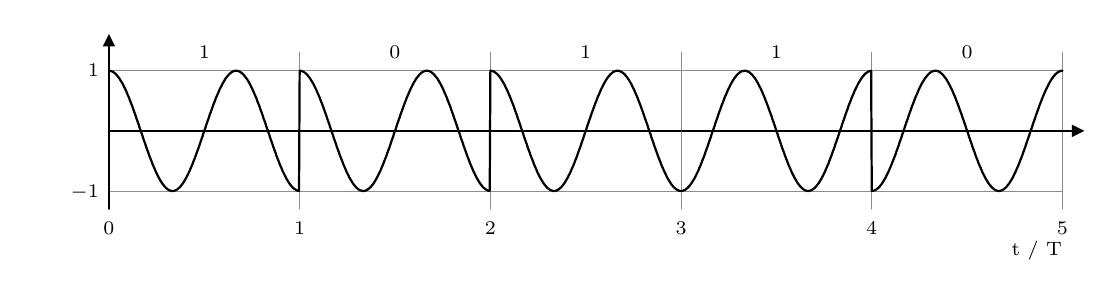
\begin{tikzpicture}[x=0.01985cm,y=-0.01985cm,line cap=round,line join=round]
\useasboundingbox (0,0) rectangle (680,150);
\path[draw=black!45,line width=0.35pt] (52,116) -- (52,16);
\path[draw=black!45,line width=0.35pt] (174,116) -- (174,16);
\path[draw=black!45,line width=0.35pt] (296,116) -- (296,16);
\path[draw=black!45,line width=0.35pt] (418,116) -- (418,16);
\path[draw=black!45,line width=0.35pt] (540,116) -- (540,16);
\path[draw=black!45,line width=0.35pt] (662,116) -- (662,16);
\path[draw=black!45,line width=0.35pt] (52,27.5) -- (662,27.5);
\path[draw=black!45,line width=0.35pt] (52,104.5) -- (662,104.5);
\path[draw=black,line width=0.7pt] (52,66) -- (670,66);
\path[fill=black,draw=none] (676,66) -- (668,62) -- (668,70) -- cycle;
\path[draw=black,line width=0.7pt] (52,116) -- (52,10);
\path[fill=black,draw=none] (52,4) -- (48,12) -- (56,12) -- cycle;
\node[anchor=base,inner sep=0pt,font=\scriptsize] at (52,132) {0};
\node[anchor=base,inner sep=0pt,font=\scriptsize] at (174,132) {1};
\node[anchor=base,inner sep=0pt,font=\scriptsize] at (296,132) {2};
\node[anchor=base,inner sep=0pt,font=\scriptsize] at (418,132) {3};
\node[anchor=base,inner sep=0pt,font=\scriptsize] at (540,132) {4};
\node[anchor=base,inner sep=0pt,font=\scriptsize] at (662,132) {5};
\node[anchor=base east,inner sep=0pt,font=\scriptsize] at (46,31.5) {1};
\node[anchor=base east,inner sep=0pt,font=\scriptsize] at (46,108.5) {$-$1};
\node[anchor=base east,inner sep=0pt,font=\scriptsize] at (662,146) {t / T};
\path[draw=black!45,line width=0.35pt,dash pattern=on 3pt off 2pt] (174,116) -- (174,16);
\path[draw=black!45,line width=0.35pt,dash pattern=on 3pt off 2pt] (296,116) -- (296,16);
\path[draw=black!45,line width=0.35pt,dash pattern=on 3pt off 2pt] (418,116) -- (418,16);
\path[draw=black!45,line width=0.35pt,dash pattern=on 3pt off 2pt] (540,116) -- (540,16);
\path[draw=black,line width=0.8pt] (52,27.5) -- (52.4,27.6) -- (52.8,27.6) -- (53.1,27.7) -- (53.5,27.8) -- (53.9,28) -- (54.3,28.1) -- (54.7,28.4) -- (55.1,28.6) -- (55.4,28.9) -- (55.8,29.2) -- (56.2,29.5) -- (56.6,29.9) -- (57,30.3) -- (57.3,30.8) -- (57.7,31.2) -- (58.1,31.7) -- (58.5,32.3) -- (58.9,32.8) -- (59.2,33.4) -- (59.6,34) -- (60,34.7) -- (60.4,35.3) -- (60.8,36) -- (61.2,36.8) -- (61.5,37.5) -- (61.9,38.3) -- (62.3,39.1) -- (62.7,39.9) -- (63.1,40.7) -- (63.4,41.6) -- (63.8,42.5) -- (64.2,43.4) -- (64.6,44.3) -- (65,45.3) -- (65.3,46.2) -- (65.7,47.2) -- (66.1,48.2) -- (66.5,49.2) -- (66.9,50.2) -- (67.3,51.3) -- (67.6,52.3) -- (68,53.4) -- (68.4,54.5) -- (68.8,55.6) -- (69.2,56.7) -- (69.5,57.8) -- (69.9,58.9) -- (70.3,60) -- (70.7,61.1) -- (71.1,62.2) -- (71.4,63.4) -- (71.8,64.5) -- (72.2,65.6) -- (72.6,66.8) -- (73,67.9) -- (73.4,69) -- (73.7,70.1) -- (74.1,71.3) -- (74.5,72.4) -- (74.9,73.5) -- (75.3,74.6) -- (75.6,75.7) -- (76,76.8) -- (76.4,77.9) -- (76.8,79) -- (77.2,80) -- (77.5,81.1) -- (77.9,82.1) -- (78.3,83.1) -- (78.7,84.1) -- (79.1,85.1) -- (79.5,86.1) -- (79.8,87.1) -- (80.2,88) -- (80.6,88.9) -- (81,89.8) -- (81.4,90.7) -- (81.7,91.5) -- (82.1,92.4) -- (82.5,93.2) -- (82.9,94) -- (83.3,94.8) -- (83.6,95.5) -- (84,96.2) -- (84.4,96.9) -- (84.8,97.6) -- (85.2,98.2) -- (85.6,98.8) -- (85.9,99.4) -- (86.3,99.9) -- (86.7,100.4) -- (87.1,100.9) -- (87.5,101.4) -- (87.8,101.8) -- (88.2,102.2) -- (88.6,102.6) -- (89,102.9) -- (89.4,103.2) -- (89.7,103.5) -- (90.1,103.7) -- (90.5,103.9) -- (90.9,104.1) -- (91.3,104.2) -- (91.7,104.3) -- (92,104.4) -- (92.4,104.5) -- (92.8,104.5) -- (93.2,104.4) -- (93.6,104.4) -- (93.9,104.3) -- (94.3,104.1) -- (94.7,104) -- (95.1,103.8) -- (95.5,103.6) -- (95.8,103.3) -- (96.2,103) -- (96.6,102.7) -- (97,102.3) -- (97.4,102) -- (97.8,101.5) -- (98.1,101.1) -- (98.5,100.6) -- (98.9,100.1) -- (99.3,99.6) -- (99.7,99) -- (100,98.4) -- (100.4,97.8) -- (100.8,97.1) -- (101.2,96.4) -- (101.6,95.7) -- (101.9,95) -- (102.3,94.2) -- (102.7,93.5) -- (103.1,92.7) -- (103.5,91.8) -- (103.9,91) -- (104.2,90.1) -- (104.6,89.2) -- (105,88.3) -- (105.4,87.4) -- (105.8,86.4) -- (106.1,85.4) -- (106.5,84.5) -- (106.9,83.5) -- (107.3,82.4) -- (107.7,81.4) -- (108,80.4) -- (108.4,79.3) -- (108.8,78.2) -- (109.2,77.2) -- (109.6,76.1) -- (110,75) -- (110.3,73.9) -- (110.7,72.8) -- (111.1,71.6) -- (111.5,70.5) -- (111.9,69.4) -- (112.2,68.3) -- (112.6,67.1) -- (113,66) -- (113.4,64.9) -- (113.8,63.7) -- (114.1,62.6) -- (114.5,61.5) -- (114.9,60.4) -- (115.3,59.2) -- (115.7,58.1) -- (116.1,57) -- (116.4,55.9) -- (116.8,54.8) -- (117.2,53.8) -- (117.6,52.7) -- (118,51.6) -- (118.3,50.6) -- (118.7,49.6) -- (119.1,48.5) -- (119.5,47.5) -- (119.9,46.6) -- (120.2,45.6) -- (120.6,44.6) -- (121,43.7) -- (121.4,42.8) -- (121.8,41.9) -- (122.2,41) -- (122.5,40.2) -- (122.9,39.3) -- (123.3,38.5) -- (123.7,37.8) -- (124.1,37) -- (124.4,36.3) -- (124.8,35.6) -- (125.2,34.9) -- (125.6,34.2) -- (126,33.6) -- (126.3,33) -- (126.7,32.4) -- (127.1,31.9) -- (127.5,31.4) -- (127.9,30.9) -- (128.3,30.5) -- (128.6,30) -- (129,29.7) -- (129.4,29.3) -- (129.8,29) -- (130.2,28.7) -- (130.5,28.4) -- (130.9,28.2) -- (131.3,28) -- (131.7,27.9) -- (132.1,27.7) -- (132.4,27.6) -- (132.8,27.6) -- (133.2,27.5) -- (133.6,27.5) -- (134,27.6) -- (134.4,27.7) -- (134.7,27.8) -- (135.1,27.9) -- (135.5,28.1) -- (135.9,28.3) -- (136.3,28.5) -- (136.6,28.8) -- (137,29.1) -- (137.4,29.4) -- (137.8,29.8) -- (138.2,30.2) -- (138.5,30.6) -- (138.9,31.1) -- (139.3,31.6) -- (139.7,32.1) -- (140.1,32.6) -- (140.5,33.2) -- (140.8,33.8) -- (141.2,34.4) -- (141.6,35.1) -- (142,35.8) -- (142.4,36.5) -- (142.7,37.2) -- (143.1,38) -- (143.5,38.8) -- (143.9,39.6) -- (144.3,40.5) -- (144.6,41.3) -- (145,42.2) -- (145.4,43.1) -- (145.8,44) -- (146.2,44.9) -- (146.6,45.9) -- (146.9,46.9) -- (147.3,47.9) -- (147.7,48.9) -- (148.1,49.9) -- (148.5,50.9) -- (148.8,52) -- (149.2,53) -- (149.6,54.1) -- (150,55.2) -- (150.4,56.3) -- (150.7,57.4) -- (151.1,58.5) -- (151.5,59.6) -- (151.9,60.7) -- (152.3,61.9) -- (152.6,63) -- (153,64.1) -- (153.4,65.2) -- (153.8,66.4) -- (154.2,67.5) -- (154.6,68.6) -- (154.9,69.8) -- (155.3,70.9) -- (155.7,72) -- (156.1,73.1) -- (156.5,74.2) -- (156.8,75.3) -- (157.2,76.4) -- (157.6,77.5) -- (158,78.6) -- (158.4,79.7) -- (158.8,80.7) -- (159.1,81.8) -- (159.5,82.8) -- (159.9,83.8) -- (160.3,84.8) -- (160.7,85.8) -- (161,86.7) -- (161.4,87.7) -- (161.8,88.6) -- (162.2,89.5) -- (162.6,90.4) -- (162.9,91.3) -- (163.3,92.1) -- (163.7,92.9) -- (164.1,93.7) -- (164.5,94.5) -- (164.9,95.2) -- (165.2,96) -- (165.6,96.7) -- (166,97.3) -- (166.4,98) -- (166.8,98.6) -- (167.1,99.2) -- (167.5,99.7) -- (167.9,100.3) -- (168.3,100.8) -- (168.7,101.2) -- (169,101.7) -- (169.4,102.1) -- (169.8,102.5) -- (170.2,102.8) -- (170.6,103.1) -- (171,103.4) -- (171.3,103.6) -- (171.7,103.9) -- (172.1,104) -- (172.5,104.2) -- (172.9,104.3) -- (173.2,104.4) -- (173.6,104.4) -- (174,27.5) -- (174.4,27.6) -- (174.8,27.6) -- (175.1,27.7) -- (175.5,27.8) -- (175.9,28) -- (176.3,28.1) -- (176.7,28.4) -- (177.1,28.6) -- (177.4,28.9) -- (177.8,29.2) -- (178.2,29.5) -- (178.6,29.9) -- (179,30.3) -- (179.3,30.8) -- (179.7,31.2) -- (180.1,31.7) -- (180.5,32.3) -- (180.9,32.8) -- (181.2,33.4) -- (181.6,34) -- (182,34.7) -- (182.4,35.3) -- (182.8,36) -- (183.2,36.8) -- (183.5,37.5) -- (183.9,38.3) -- (184.3,39.1) -- (184.7,39.9) -- (185.1,40.7) -- (185.4,41.6) -- (185.8,42.5) -- (186.2,43.4) -- (186.6,44.3) -- (187,45.3) -- (187.3,46.2) -- (187.7,47.2) -- (188.1,48.2) -- (188.5,49.2) -- (188.9,50.2) -- (189.3,51.3) -- (189.6,52.3) -- (190,53.4) -- (190.4,54.5) -- (190.8,55.6) -- (191.2,56.7) -- (191.5,57.8) -- (191.9,58.9) -- (192.3,60) -- (192.7,61.1) -- (193.1,62.2) -- (193.4,63.4) -- (193.8,64.5) -- (194.2,65.6) -- (194.6,66.8) -- (195,67.9) -- (195.4,69) -- (195.7,70.1) -- (196.1,71.3) -- (196.5,72.4) -- (196.9,73.5) -- (197.3,74.6) -- (197.6,75.7) -- (198,76.8) -- (198.4,77.9) -- (198.8,79) -- (199.2,80) -- (199.5,81.1) -- (199.9,82.1) -- (200.3,83.1) -- (200.7,84.1) -- (201.1,85.1) -- (201.5,86.1) -- (201.8,87.1) -- (202.2,88) -- (202.6,88.9) -- (203,89.8) -- (203.4,90.7) -- (203.7,91.5) -- (204.1,92.4) -- (204.5,93.2) -- (204.9,94) -- (205.3,94.8) -- (205.6,95.5) -- (206,96.2) -- (206.4,96.9) -- (206.8,97.6) -- (207.2,98.2) -- (207.6,98.8) -- (207.9,99.4) -- (208.3,99.9) -- (208.7,100.4) -- (209.1,100.9) -- (209.5,101.4) -- (209.8,101.8) -- (210.2,102.2) -- (210.6,102.6) -- (211,102.9) -- (211.4,103.2) -- (211.7,103.5) -- (212.1,103.7) -- (212.5,103.9) -- (212.9,104.1) -- (213.3,104.2) -- (213.7,104.3) -- (214,104.4) -- (214.4,104.5) -- (214.8,104.5) -- (215.2,104.4) -- (215.6,104.4) -- (215.9,104.3) -- (216.3,104.1) -- (216.7,104) -- (217.1,103.8) -- (217.5,103.6) -- (217.8,103.3) -- (218.2,103) -- (218.6,102.7) -- (219,102.3) -- (219.4,102) -- (219.8,101.5) -- (220.1,101.1) -- (220.5,100.6) -- (220.9,100.1) -- (221.3,99.6) -- (221.7,99) -- (222,98.4) -- (222.4,97.8) -- (222.8,97.1) -- (223.2,96.4) -- (223.6,95.7) -- (223.9,95) -- (224.3,94.2) -- (224.7,93.5) -- (225.1,92.7) -- (225.5,91.8) -- (225.9,91) -- (226.2,90.1) -- (226.6,89.2) -- (227,88.3) -- (227.4,87.4) -- (227.8,86.4) -- (228.1,85.4) -- (228.5,84.5) -- (228.9,83.5) -- (229.3,82.4) -- (229.7,81.4) -- (230,80.4) -- (230.4,79.3) -- (230.8,78.2) -- (231.2,77.2) -- (231.6,76.1) -- (232,75) -- (232.3,73.9) -- (232.7,72.8) -- (233.1,71.6) -- (233.5,70.5) -- (233.9,69.4) -- (234.2,68.3) -- (234.6,67.1) -- (235,66) -- (235.4,64.9) -- (235.8,63.7) -- (236.1,62.6) -- (236.5,61.5) -- (236.9,60.4) -- (237.3,59.2) -- (237.7,58.1) -- (238.1,57) -- (238.4,55.9) -- (238.8,54.8) -- (239.2,53.8) -- (239.6,52.7) -- (240,51.6) -- (240.3,50.6) -- (240.7,49.6) -- (241.1,48.5) -- (241.5,47.5) -- (241.9,46.6) -- (242.2,45.6) -- (242.6,44.6) -- (243,43.7) -- (243.4,42.8) -- (243.8,41.9) -- (244.2,41) -- (244.5,40.2) -- (244.9,39.3) -- (245.3,38.5) -- (245.7,37.8) -- (246.1,37) -- (246.4,36.3) -- (246.8,35.6) -- (247.2,34.9) -- (247.6,34.2) -- (248,33.6) -- (248.3,33) -- (248.7,32.4) -- (249.1,31.9) -- (249.5,31.4) -- (249.9,30.9) -- (250.3,30.5) -- (250.6,30) -- (251,29.7) -- (251.4,29.3) -- (251.8,29) -- (252.2,28.7) -- (252.5,28.4) -- (252.9,28.2) -- (253.3,28) -- (253.7,27.9) -- (254.1,27.7) -- (254.4,27.6) -- (254.8,27.6) -- (255.2,27.5) -- (255.6,27.5) -- (256,27.6) -- (256.4,27.7) -- (256.7,27.8) -- (257.1,27.9) -- (257.5,28.1) -- (257.9,28.3) -- (258.3,28.5) -- (258.6,28.8) -- (259,29.1) -- (259.4,29.4) -- (259.8,29.8) -- (260.2,30.2) -- (260.5,30.6) -- (260.9,31.1) -- (261.3,31.6) -- (261.7,32.1) -- (262.1,32.6) -- (262.5,33.2) -- (262.8,33.8) -- (263.2,34.4) -- (263.6,35.1) -- (264,35.8) -- (264.4,36.5) -- (264.7,37.2) -- (265.1,38) -- (265.5,38.8) -- (265.9,39.6) -- (266.3,40.5) -- (266.6,41.3) -- (267,42.2) -- (267.4,43.1) -- (267.8,44) -- (268.2,44.9) -- (268.5,45.9) -- (268.9,46.9) -- (269.3,47.9) -- (269.7,48.9) -- (270.1,49.9) -- (270.5,50.9) -- (270.8,52) -- (271.2,53) -- (271.6,54.1) -- (272,55.2) -- (272.4,56.3) -- (272.7,57.4) -- (273.1,58.5) -- (273.5,59.6) -- (273.9,60.7) -- (274.3,61.9) -- (274.7,63) -- (275,64.1) -- (275.4,65.2) -- (275.8,66.4) -- (276.2,67.5) -- (276.6,68.6) -- (276.9,69.8) -- (277.3,70.9) -- (277.7,72) -- (278.1,73.1) -- (278.5,74.2) -- (278.8,75.3) -- (279.2,76.4) -- (279.6,77.5) -- (280,78.6) -- (280.4,79.7) -- (280.8,80.7) -- (281.1,81.8) -- (281.5,82.8) -- (281.9,83.8) -- (282.3,84.8) -- (282.7,85.8) -- (283,86.7) -- (283.4,87.7) -- (283.8,88.6) -- (284.2,89.5) -- (284.6,90.4) -- (284.9,91.3) -- (285.3,92.1) -- (285.7,92.9) -- (286.1,93.7) -- (286.5,94.5) -- (286.9,95.2) -- (287.2,96) -- (287.6,96.7) -- (288,97.3) -- (288.4,98) -- (288.8,98.6) -- (289.1,99.2) -- (289.5,99.7) -- (289.9,100.3) -- (290.3,100.8) -- (290.7,101.2) -- (291,101.7) -- (291.4,102.1) -- (291.8,102.5) -- (292.2,102.8) -- (292.6,103.1) -- (293,103.4) -- (293.3,103.6) -- (293.7,103.9) -- (294.1,104) -- (294.5,104.2) -- (294.9,104.3) -- (295.2,104.4) -- (295.6,104.4) -- (296,27.5) -- (296.4,27.6) -- (296.8,27.6) -- (297.1,27.7) -- (297.5,27.8) -- (297.9,28) -- (298.3,28.1) -- (298.7,28.4) -- (299,28.6) -- (299.4,28.9) -- (299.8,29.2) -- (300.2,29.5) -- (300.6,29.9) -- (301,30.3) -- (301.3,30.8) -- (301.7,31.2) -- (302.1,31.7) -- (302.5,32.3) -- (302.9,32.8) -- (303.2,33.4) -- (303.6,34) -- (304,34.7) -- (304.4,35.3) -- (304.8,36) -- (305.2,36.8) -- (305.5,37.5) -- (305.9,38.3) -- (306.3,39.1) -- (306.7,39.9) -- (307.1,40.7) -- (307.4,41.6) -- (307.8,42.5) -- (308.2,43.4) -- (308.6,44.3) -- (309,45.3) -- (309.3,46.2) -- (309.7,47.2) -- (310.1,48.2) -- (310.5,49.2) -- (310.9,50.2) -- (311.3,51.3) -- (311.6,52.3) -- (312,53.4) -- (312.4,54.5) -- (312.8,55.6) -- (313.2,56.7) -- (313.5,57.8) -- (313.9,58.9) -- (314.3,60) -- (314.7,61.1) -- (315.1,62.2) -- (315.4,63.4) -- (315.8,64.5) -- (316.2,65.6) -- (316.6,66.8) -- (317,67.9) -- (317.3,69) -- (317.7,70.1) -- (318.1,71.3) -- (318.5,72.4) -- (318.9,73.5) -- (319.3,74.6) -- (319.6,75.7) -- (320,76.8) -- (320.4,77.9) -- (320.8,79) -- (321.2,80) -- (321.5,81.1) -- (321.9,82.1) -- (322.3,83.1) -- (322.7,84.1) -- (323.1,85.1) -- (323.5,86.1) -- (323.8,87.1) -- (324.2,88) -- (324.6,88.9) -- (325,89.8) -- (325.4,90.7) -- (325.7,91.5) -- (326.1,92.4) -- (326.5,93.2) -- (326.9,94) -- (327.3,94.8) -- (327.6,95.5) -- (328,96.2) -- (328.4,96.9) -- (328.8,97.6) -- (329.2,98.2) -- (329.5,98.8) -- (329.9,99.4) -- (330.3,99.9) -- (330.7,100.4) -- (331.1,100.9) -- (331.5,101.4) -- (331.8,101.8) -- (332.2,102.2) -- (332.6,102.6) -- (333,102.9) -- (333.4,103.2) -- (333.7,103.5) -- (334.1,103.7) -- (334.5,103.9) -- (334.9,104.1) -- (335.3,104.2) -- (335.7,104.3) -- (336,104.4) -- (336.4,104.5) -- (336.8,104.5) -- (337.2,104.4) -- (337.6,104.4) -- (337.9,104.3) -- (338.3,104.1) -- (338.7,104) -- (339.1,103.8) -- (339.5,103.6) -- (339.8,103.3) -- (340.2,103) -- (340.6,102.7) -- (341,102.3) -- (341.4,102) -- (341.8,101.5) -- (342.1,101.1) -- (342.5,100.6) -- (342.9,100.1) -- (343.3,99.6) -- (343.7,99) -- (344,98.4) -- (344.4,97.8) -- (344.8,97.1) -- (345.2,96.4) -- (345.6,95.7) -- (345.9,95) -- (346.3,94.2) -- (346.7,93.5) -- (347.1,92.7) -- (347.5,91.8) -- (347.8,91) -- (348.2,90.1) -- (348.6,89.2) -- (349,88.3) -- (349.4,87.4) -- (349.8,86.4) -- (350.1,85.4) -- (350.5,84.5) -- (350.9,83.5) -- (351.3,82.4) -- (351.7,81.4) -- (352,80.4) -- (352.4,79.3) -- (352.8,78.2) -- (353.2,77.2) -- (353.6,76.1) -- (354,75) -- (354.3,73.9) -- (354.7,72.8) -- (355.1,71.6) -- (355.5,70.5) -- (355.9,69.4) -- (356.2,68.3) -- (356.6,67.1) -- (357,66) -- (357.4,64.9) -- (357.8,63.7) -- (358.1,62.6) -- (358.5,61.5) -- (358.9,60.4) -- (359.3,59.2) -- (359.7,58.1) -- (360.1,57) -- (360.4,55.9) -- (360.8,54.8) -- (361.2,53.8) -- (361.6,52.7) -- (362,51.6) -- (362.3,50.6) -- (362.7,49.6) -- (363.1,48.5) -- (363.5,47.5) -- (363.9,46.6) -- (364.2,45.6) -- (364.6,44.6) -- (365,43.7) -- (365.4,42.8) -- (365.8,41.9) -- (366.2,41) -- (366.5,40.2) -- (366.9,39.3) -- (367.3,38.5) -- (367.7,37.8) -- (368.1,37) -- (368.4,36.3) -- (368.8,35.6) -- (369.2,34.9) -- (369.6,34.2) -- (370,33.6) -- (370.3,33) -- (370.7,32.4) -- (371.1,31.9) -- (371.5,31.4) -- (371.9,30.9) -- (372.3,30.5) -- (372.6,30) -- (373,29.7) -- (373.4,29.3) -- (373.8,29) -- (374.2,28.7) -- (374.5,28.4) -- (374.9,28.2) -- (375.3,28) -- (375.7,27.9) -- (376.1,27.7) -- (376.4,27.6) -- (376.8,27.6) -- (377.2,27.5) -- (377.6,27.5) -- (378,27.6) -- (378.3,27.7) -- (378.7,27.8) -- (379.1,27.9) -- (379.5,28.1) -- (379.9,28.3) -- (380.3,28.5) -- (380.6,28.8) -- (381,29.1) -- (381.4,29.4) -- (381.8,29.8) -- (382.2,30.2) -- (382.5,30.6) -- (382.9,31.1) -- (383.3,31.6) -- (383.7,32.1) -- (384.1,32.6) -- (384.5,33.2) -- (384.8,33.8) -- (385.2,34.4) -- (385.6,35.1) -- (386,35.8) -- (386.4,36.5) -- (386.7,37.2) -- (387.1,38) -- (387.5,38.8) -- (387.9,39.6) -- (388.3,40.5) -- (388.6,41.3) -- (389,42.2) -- (389.4,43.1) -- (389.8,44) -- (390.2,44.9) -- (390.5,45.9) -- (390.9,46.9) -- (391.3,47.9) -- (391.7,48.9) -- (392.1,49.9) -- (392.5,50.9) -- (392.8,52) -- (393.2,53) -- (393.6,54.1) -- (394,55.2) -- (394.4,56.3) -- (394.7,57.4) -- (395.1,58.5) -- (395.5,59.6) -- (395.9,60.7) -- (396.3,61.9) -- (396.7,63) -- (397,64.1) -- (397.4,65.2) -- (397.8,66.4) -- (398.2,67.5) -- (398.6,68.6) -- (398.9,69.8) -- (399.3,70.9) -- (399.7,72) -- (400.1,73.1) -- (400.5,74.2) -- (400.8,75.3) -- (401.2,76.4) -- (401.6,77.5) -- (402,78.6) -- (402.4,79.7) -- (402.8,80.7) -- (403.1,81.8) -- (403.5,82.8) -- (403.9,83.8) -- (404.3,84.8) -- (404.7,85.8) -- (405,86.7) -- (405.4,87.7) -- (405.8,88.6) -- (406.2,89.5) -- (406.6,90.4) -- (406.9,91.3) -- (407.3,92.1) -- (407.7,92.9) -- (408.1,93.7) -- (408.5,94.5) -- (408.8,95.2) -- (409.2,96) -- (409.6,96.7) -- (410,97.3) -- (410.4,98) -- (410.8,98.6) -- (411.1,99.2) -- (411.5,99.7) -- (411.9,100.3) -- (412.3,100.8) -- (412.7,101.2) -- (413,101.7) -- (413.4,102.1) -- (413.8,102.5) -- (414.2,102.8) -- (414.6,103.1) -- (415,103.4) -- (415.3,103.6) -- (415.7,103.9) -- (416.1,104) -- (416.5,104.2) -- (416.9,104.3) -- (417.2,104.4) -- (417.6,104.4) -- (418,104.5) -- (418.4,104.4) -- (418.8,104.4) -- (419.1,104.3) -- (419.5,104.2) -- (419.9,104) -- (420.3,103.9) -- (420.7,103.6) -- (421.1,103.4) -- (421.4,103.1) -- (421.8,102.8) -- (422.2,102.5) -- (422.6,102.1) -- (423,101.7) -- (423.3,101.2) -- (423.7,100.8) -- (424.1,100.3) -- (424.5,99.7) -- (424.9,99.2) -- (425.2,98.6) -- (425.6,98) -- (426,97.3) -- (426.4,96.7) -- (426.8,96) -- (427.2,95.2) -- (427.5,94.5) -- (427.9,93.7) -- (428.3,92.9) -- (428.7,92.1) -- (429.1,91.3) -- (429.4,90.4) -- (429.8,89.5) -- (430.2,88.6) -- (430.6,87.7) -- (431,86.7) -- (431.3,85.8) -- (431.7,84.8) -- (432.1,83.8) -- (432.5,82.8) -- (432.9,81.8) -- (433.3,80.7) -- (433.6,79.7) -- (434,78.6) -- (434.4,77.5) -- (434.8,76.4) -- (435.2,75.3) -- (435.5,74.2) -- (435.9,73.1) -- (436.3,72) -- (436.7,70.9) -- (437.1,69.8) -- (437.4,68.6) -- (437.8,67.5) -- (438.2,66.4) -- (438.6,65.2) -- (439,64.1) -- (439.4,63) -- (439.7,61.9) -- (440.1,60.7) -- (440.5,59.6) -- (440.9,58.5) -- (441.3,57.4) -- (441.6,56.3) -- (442,55.2) -- (442.4,54.1) -- (442.8,53) -- (443.2,52) -- (443.5,50.9) -- (443.9,49.9) -- (444.3,48.9) -- (444.7,47.9) -- (445.1,46.9) -- (445.5,45.9) -- (445.8,44.9) -- (446.2,44) -- (446.6,43.1) -- (447,42.2) -- (447.4,41.3) -- (447.7,40.5) -- (448.1,39.6) -- (448.5,38.8) -- (448.9,38) -- (449.3,37.2) -- (449.6,36.5) -- (450,35.8) -- (450.4,35.1) -- (450.8,34.4) -- (451.2,33.8) -- (451.6,33.2) -- (451.9,32.6) -- (452.3,32.1) -- (452.7,31.6) -- (453.1,31.1) -- (453.5,30.6) -- (453.8,30.2) -- (454.2,29.8) -- (454.6,29.4) -- (455,29.1) -- (455.4,28.8) -- (455.7,28.5) -- (456.1,28.3) -- (456.5,28.1) -- (456.9,27.9) -- (457.3,27.8) -- (457.7,27.7) -- (458,27.6) -- (458.4,27.5) -- (458.8,27.5) -- (459.2,27.6) -- (459.6,27.6) -- (459.9,27.7) -- (460.3,27.9) -- (460.7,28) -- (461.1,28.2) -- (461.5,28.4) -- (461.8,28.7) -- (462.2,29) -- (462.6,29.3) -- (463,29.7) -- (463.4,30) -- (463.8,30.5) -- (464.1,30.9) -- (464.5,31.4) -- (464.9,31.9) -- (465.3,32.4) -- (465.7,33) -- (466,33.6) -- (466.4,34.2) -- (466.8,34.9) -- (467.2,35.6) -- (467.6,36.3) -- (467.9,37) -- (468.3,37.8) -- (468.7,38.5) -- (469.1,39.3) -- (469.5,40.2) -- (469.9,41) -- (470.2,41.9) -- (470.6,42.8) -- (471,43.7) -- (471.4,44.6) -- (471.8,45.6) -- (472.1,46.6) -- (472.5,47.5) -- (472.9,48.5) -- (473.3,49.6) -- (473.7,50.6) -- (474,51.6) -- (474.4,52.7) -- (474.8,53.8) -- (475.2,54.8) -- (475.6,55.9) -- (476,57) -- (476.3,58.1) -- (476.7,59.2) -- (477.1,60.4) -- (477.5,61.5) -- (477.9,62.6) -- (478.2,63.7) -- (478.6,64.9) -- (479,66) -- (479.4,67.1) -- (479.8,68.3) -- (480.1,69.4) -- (480.5,70.5) -- (480.9,71.6) -- (481.3,72.8) -- (481.7,73.9) -- (482.1,75) -- (482.4,76.1) -- (482.8,77.2) -- (483.2,78.2) -- (483.6,79.3) -- (484,80.4) -- (484.3,81.4) -- (484.7,82.4) -- (485.1,83.5) -- (485.5,84.5) -- (485.9,85.4) -- (486.2,86.4) -- (486.6,87.4) -- (487,88.3) -- (487.4,89.2) -- (487.8,90.1) -- (488.2,91) -- (488.5,91.8) -- (488.9,92.7) -- (489.3,93.5) -- (489.7,94.2) -- (490.1,95) -- (490.4,95.7) -- (490.8,96.4) -- (491.2,97.1) -- (491.6,97.8) -- (492,98.4) -- (492.3,99) -- (492.7,99.6) -- (493.1,100.1) -- (493.5,100.6) -- (493.9,101.1) -- (494.3,101.5) -- (494.6,102) -- (495,102.3) -- (495.4,102.7) -- (495.8,103) -- (496.2,103.3) -- (496.5,103.6) -- (496.9,103.8) -- (497.3,104) -- (497.7,104.1) -- (498.1,104.3) -- (498.4,104.4) -- (498.8,104.4) -- (499.2,104.5) -- (499.6,104.5) -- (500,104.4) -- (500.4,104.3) -- (500.7,104.2) -- (501.1,104.1) -- (501.5,103.9) -- (501.9,103.7) -- (502.3,103.5) -- (502.6,103.2) -- (503,102.9) -- (503.4,102.6) -- (503.8,102.2) -- (504.2,101.8) -- (504.5,101.4) -- (504.9,100.9) -- (505.3,100.4) -- (505.7,99.9) -- (506.1,99.4) -- (506.5,98.8) -- (506.8,98.2) -- (507.2,97.6) -- (507.6,96.9) -- (508,96.2) -- (508.4,95.5) -- (508.7,94.8) -- (509.1,94) -- (509.5,93.2) -- (509.9,92.4) -- (510.3,91.5) -- (510.6,90.7) -- (511,89.8) -- (511.4,88.9) -- (511.8,88) -- (512.2,87.1) -- (512.6,86.1) -- (512.9,85.1) -- (513.3,84.1) -- (513.7,83.1) -- (514.1,82.1) -- (514.5,81.1) -- (514.8,80) -- (515.2,79) -- (515.6,77.9) -- (516,76.8) -- (516.4,75.7) -- (516.7,74.6) -- (517.1,73.5) -- (517.5,72.4) -- (517.9,71.3) -- (518.3,70.1) -- (518.7,69) -- (519,67.9) -- (519.4,66.8) -- (519.8,65.6) -- (520.2,64.5) -- (520.6,63.4) -- (520.9,62.2) -- (521.3,61.1) -- (521.7,60) -- (522.1,58.9) -- (522.5,57.8) -- (522.8,56.7) -- (523.2,55.6) -- (523.6,54.5) -- (524,53.4) -- (524.4,52.3) -- (524.8,51.3) -- (525.1,50.2) -- (525.5,49.2) -- (525.9,48.2) -- (526.3,47.2) -- (526.7,46.2) -- (527,45.3) -- (527.4,44.3) -- (527.8,43.4) -- (528.2,42.5) -- (528.6,41.6) -- (528.9,40.7) -- (529.3,39.9) -- (529.7,39.1) -- (530.1,38.3) -- (530.5,37.5) -- (530.8,36.8) -- (531.2,36) -- (531.6,35.3) -- (532,34.7) -- (532.4,34) -- (532.8,33.4) -- (533.1,32.8) -- (533.5,32.3) -- (533.9,31.7) -- (534.3,31.2) -- (534.7,30.8) -- (535,30.3) -- (535.4,29.9) -- (535.8,29.5) -- (536.2,29.2) -- (536.6,28.9) -- (537,28.6) -- (537.3,28.4) -- (537.7,28.1) -- (538.1,28) -- (538.5,27.8) -- (538.9,27.7) -- (539.2,27.6) -- (539.6,27.6) -- (540,104.5) -- (540.4,104.4) -- (540.8,104.4) -- (541.1,104.3) -- (541.5,104.2) -- (541.9,104) -- (542.3,103.9) -- (542.7,103.6) -- (543.1,103.4) -- (543.4,103.1) -- (543.8,102.8) -- (544.2,102.5) -- (544.6,102.1) -- (545,101.7) -- (545.3,101.2) -- (545.7,100.8) -- (546.1,100.3) -- (546.5,99.7) -- (546.9,99.2) -- (547.2,98.6) -- (547.6,98) -- (548,97.3) -- (548.4,96.7) -- (548.8,96) -- (549.2,95.2) -- (549.5,94.5) -- (549.9,93.7) -- (550.3,92.9) -- (550.7,92.1) -- (551.1,91.3) -- (551.4,90.4) -- (551.8,89.5) -- (552.2,88.6) -- (552.6,87.7) -- (553,86.7) -- (553.3,85.8) -- (553.7,84.8) -- (554.1,83.8) -- (554.5,82.8) -- (554.9,81.8) -- (555.3,80.7) -- (555.6,79.7) -- (556,78.6) -- (556.4,77.5) -- (556.8,76.4) -- (557.2,75.3) -- (557.5,74.2) -- (557.9,73.1) -- (558.3,72) -- (558.7,70.9) -- (559.1,69.8) -- (559.4,68.6) -- (559.8,67.5) -- (560.2,66.4) -- (560.6,65.2) -- (561,64.1) -- (561.3,63) -- (561.7,61.9) -- (562.1,60.7) -- (562.5,59.6) -- (562.9,58.5) -- (563.3,57.4) -- (563.6,56.3) -- (564,55.2) -- (564.4,54.1) -- (564.8,53) -- (565.2,52) -- (565.5,50.9) -- (565.9,49.9) -- (566.3,48.9) -- (566.7,47.9) -- (567.1,46.9) -- (567.4,45.9) -- (567.8,44.9) -- (568.2,44) -- (568.6,43.1) -- (569,42.2) -- (569.4,41.3) -- (569.7,40.5) -- (570.1,39.6) -- (570.5,38.8) -- (570.9,38) -- (571.3,37.2) -- (571.6,36.5) -- (572,35.8) -- (572.4,35.1) -- (572.8,34.4) -- (573.2,33.8) -- (573.6,33.2) -- (573.9,32.6) -- (574.3,32.1) -- (574.7,31.6) -- (575.1,31.1) -- (575.5,30.6) -- (575.8,30.2) -- (576.2,29.8) -- (576.6,29.4) -- (577,29.1) -- (577.4,28.8) -- (577.7,28.5) -- (578.1,28.3) -- (578.5,28.1) -- (578.9,27.9) -- (579.3,27.8) -- (579.7,27.7) -- (580,27.6) -- (580.4,27.5) -- (580.8,27.5) -- (581.2,27.6) -- (581.6,27.6) -- (581.9,27.7) -- (582.3,27.9) -- (582.7,28) -- (583.1,28.2) -- (583.5,28.4) -- (583.8,28.7) -- (584.2,29) -- (584.6,29.3) -- (585,29.7) -- (585.4,30) -- (585.8,30.5) -- (586.1,30.9) -- (586.5,31.4) -- (586.9,31.9) -- (587.3,32.4) -- (587.7,33) -- (588,33.6) -- (588.4,34.2) -- (588.8,34.9) -- (589.2,35.6) -- (589.6,36.3) -- (589.9,37) -- (590.3,37.8) -- (590.7,38.5) -- (591.1,39.3) -- (591.5,40.2) -- (591.9,41) -- (592.2,41.9) -- (592.6,42.8) -- (593,43.7) -- (593.4,44.6) -- (593.8,45.6) -- (594.1,46.6) -- (594.5,47.5) -- (594.9,48.5) -- (595.3,49.6) -- (595.7,50.6) -- (596,51.6) -- (596.4,52.7) -- (596.8,53.8) -- (597.2,54.8) -- (597.6,55.9) -- (597.9,57) -- (598.3,58.1) -- (598.7,59.2) -- (599.1,60.4) -- (599.5,61.5) -- (599.9,62.6) -- (600.2,63.7) -- (600.6,64.9) -- (601,66) -- (601.4,67.1) -- (601.8,68.3) -- (602.1,69.4) -- (602.5,70.5) -- (602.9,71.6) -- (603.3,72.8) -- (603.7,73.9) -- (604.1,75) -- (604.4,76.1) -- (604.8,77.2) -- (605.2,78.2) -- (605.6,79.3) -- (606,80.4) -- (606.3,81.4) -- (606.7,82.4) -- (607.1,83.5) -- (607.5,84.5) -- (607.9,85.4) -- (608.2,86.4) -- (608.6,87.4) -- (609,88.3) -- (609.4,89.2) -- (609.8,90.1) -- (610.2,91) -- (610.5,91.8) -- (610.9,92.7) -- (611.3,93.5) -- (611.7,94.2) -- (612.1,95) -- (612.4,95.7) -- (612.8,96.4) -- (613.2,97.1) -- (613.6,97.8) -- (614,98.4) -- (614.3,99) -- (614.7,99.6) -- (615.1,100.1) -- (615.5,100.6) -- (615.9,101.1) -- (616.3,101.5) -- (616.6,102) -- (617,102.3) -- (617.4,102.7) -- (617.8,103) -- (618.2,103.3) -- (618.5,103.6) -- (618.9,103.8) -- (619.3,104) -- (619.7,104.1) -- (620.1,104.3) -- (620.4,104.4) -- (620.8,104.4) -- (621.2,104.5) -- (621.6,104.5) -- (622,104.4) -- (622.3,104.3) -- (622.7,104.2) -- (623.1,104.1) -- (623.5,103.9) -- (623.9,103.7) -- (624.3,103.5) -- (624.6,103.2) -- (625,102.9) -- (625.4,102.6) -- (625.8,102.2) -- (626.2,101.8) -- (626.5,101.4) -- (626.9,100.9) -- (627.3,100.4) -- (627.7,99.9) -- (628.1,99.4) -- (628.4,98.8) -- (628.8,98.2) -- (629.2,97.6) -- (629.6,96.9) -- (630,96.2) -- (630.4,95.5) -- (630.7,94.8) -- (631.1,94) -- (631.5,93.2) -- (631.9,92.4) -- (632.3,91.5) -- (632.6,90.7) -- (633,89.8) -- (633.4,88.9) -- (633.8,88) -- (634.2,87.1) -- (634.6,86.1) -- (634.9,85.1) -- (635.3,84.1) -- (635.7,83.1) -- (636.1,82.1) -- (636.5,81.1) -- (636.8,80) -- (637.2,79) -- (637.6,77.9) -- (638,76.8) -- (638.4,75.7) -- (638.7,74.6) -- (639.1,73.5) -- (639.5,72.4) -- (639.9,71.3) -- (640.3,70.1) -- (640.7,69) -- (641,67.9) -- (641.4,66.8) -- (641.8,65.6) -- (642.2,64.5) -- (642.6,63.4) -- (642.9,62.2) -- (643.3,61.1) -- (643.7,60) -- (644.1,58.9) -- (644.5,57.8) -- (644.8,56.7) -- (645.2,55.6) -- (645.6,54.5) -- (646,53.4) -- (646.4,52.3) -- (646.8,51.3) -- (647.1,50.2) -- (647.5,49.2) -- (647.9,48.2) -- (648.3,47.2) -- (648.7,46.2) -- (649,45.3) -- (649.4,44.3) -- (649.8,43.4) -- (650.2,42.5) -- (650.6,41.6) -- (650.9,40.7) -- (651.3,39.9) -- (651.7,39.1) -- (652.1,38.3) -- (652.5,37.5) -- (652.9,36.8) -- (653.2,36) -- (653.6,35.3) -- (654,34.7) -- (654.4,34) -- (654.8,33.4) -- (655.1,32.8) -- (655.5,32.3) -- (655.9,31.7) -- (656.3,31.2) -- (656.7,30.8) -- (657,30.3) -- (657.4,29.9) -- (657.8,29.5) -- (658.2,29.2) -- (658.6,28.9) -- (658.9,28.6) -- (659.3,28.4) -- (659.7,28.1) -- (660.1,28) -- (660.5,27.8) -- (660.9,27.7) -- (661.2,27.6) -- (661.6,27.6) -- (662,27.5);
\node[anchor=base,inner sep=0pt,font=\scriptsize] at (113,20) {1};
\node[anchor=base,inner sep=0pt,font=\scriptsize] at (235,20) {0};
\node[anchor=base,inner sep=0pt,font=\scriptsize] at (357,20) {1};
\node[anchor=base,inner sep=0pt,font=\scriptsize] at (479,20) {1};
\node[anchor=base,inner sep=0pt,font=\scriptsize] at (601,20) {0};
\end{tikzpicture}\end{center}
\begin{itemize}
\item Bitenként 1,5 vivőperiódus. 1-nél $+\cos$, 0-nál $-\cos$: a szaggatott bithatáron a jel előjelet vált, ha a bit változik.
\item Mivel a bitidő nem egész számú periódus, a fázisugrás a vivő más-más pontjára esik.
\end{itemize}
\end{rajz}
\begin{eredmeny}

\begin{center}\adjustbox{max width=\linewidth}{$\displaystyle 1\to+\cos,\ 0\to-\cos\qquad\text{bitenként }1{,}5\ \text{vivőperiódus, összesen }7{,}5$}\end{center}
\end{eredmeny}
\begin{tipp}[Ellenőrzés]
\begin{itemize}
\item A vivő szinuszos (a Moodle-válasz „négyszögjel”-et írt).
\end{itemize}
\end{tipp}


% ------------------------------------------------------------------
\section{\texorpdfstring{7.2. feladat: FSK/MSK: 22,2 és 24,2 kHz}{7.2. feladat: FSK/MSK: 22,2 és 24,2 kHz}}\label{ai7_02}
\setcounter{lepes}{0}
\begin{feladat}{7.2. feladat}
Bináris FSK (MSK), $f_1=22{,}2$ kHz, $f_2=24{,}2$ kHz. a) Frekvencialöket? b) Vivőfrekvencia? c) MSK-nál a bitsebesség? d) Miért jobb az MSK, hol használnak GMSK-t?

{\footnotesize\sffamily Forrás: ALL-IN 12., 27\ldots{}28., 52. oldal $\cdot$ ai2020\_06\_02\_Q3, ai2016\_06\_07\_4, ai2014\_12\_15\_1. Címkék: vizsga}
\end{feladat}
\begin{keresunk}
\begin{itemize}
\item a) $f_D$ (frekvencialöket)
\item b) $F$ (vivőfrekvencia)
\item c) $1/T$
\item d) indoklás
\end{itemize}
\end{keresunk}
\begin{jeloles}
\begin{jeltabla}
$f_D$ & frekvencialöket & \emph{keresett}\\
$F$ & vivőfrekvencia & \emph{keresett}\\
$T$ & jelzési (bit-) idő & \emph{keresett}\\
$f_1$ & az egyik jelzőfrekvencia & \\
$f_2$ & a másik jelzőfrekvencia & \\
\end{jeltabla}
\par\smallskip\textbf{Adott még:}
\begin{itemize}
\item a két jelzőfrekvencia: 22,2 és 24,2 kHz
\end{itemize}
\end{jeloles}

\lepes{a), b) Löket és vivő}
FSK-nál a vivő a két jelzőfrekvencia átlaga, a löket a különbségük fele.

\begin{center}\adjustbox{max width=\linewidth}{$\displaystyle f_D=\frac{24{,}2-22{,}2}{2}=1\ \text{kHz}\qquad F=\frac{22{,}2+24{,}2}{2}=23{,}2\ \text{kHz}$}\end{center}
\jegyzet{definíció}{}

\lepes{c) Bitsebesség MSK-nál}
MSK-feltétel: $f_DT=1/4$.

\begin{center}\adjustbox{max width=\linewidth}{$\displaystyle T=\frac{1}{4f_D}=\frac1{4\ \text{kHz}}=0{,}25\ \text{ms}\ \Rightarrow\ \frac1T=4\ \text{kbit/s}$}\end{center}
\jegyzet{tétel}{}

\lepes{d) Miért jobb?}
A fázis folytonos (nincs ugrás a bithatáron), és a két frekvencia a lehető legközelebb van egymáshoz úgy, hogy még ortogonálisak: kompakt, gyorsan lecsengő spektrum, állandó burkoló. A GMSK (Gauss-szűrővel előszűrt MSK) a GSM modulációja.
\begin{eredmeny}

\begin{center}\adjustbox{max width=\linewidth}{$\displaystyle \text{a) }f_D=1\ \text{kHz}\qquad\text{b) }F=23{,}2\ \text{kHz}\qquad\text{c) }4\ \text{kbit/s}\qquad\text{d) GSM}$}\end{center}
\end{eredmeny}


% ------------------------------------------------------------------
\section{\texorpdfstring{7.3. feladat: FSK 150 kHz-en, 50 kHz-es lökettel, majd MSK}{7.3. feladat: FSK 150 kHz-en, 50 kHz-es lökettel, majd MSK}}\label{ai7_03}
\setcounter{lepes}{0}
\begin{feladat}{7.3. feladat}
FSK, $F=150$ kHz, $f_D=50$ kHz, $T=20$ \textmu{}s, amplitúdó 2 V. a) $f_0$, $f_1$, rajz a 0110 bitsorra. b) Sávszélesség? c) Mit kell változtatni MSK-hoz? d) Rajz MSK-ra.

{\footnotesize\sffamily Forrás: ALL-IN 36\ldots{}39. oldal $\cdot$ ai2015\_12\_16\_4b. Címkék: vizsga, javítás}
\end{feladat}
\begin{keresunk}
\begin{itemize}
\item a) $f_0$ (a 0-s bit frekvenciája), $f_1$ (az 1-es bit frekvenciája)
\item b) $B_v$ (a modulált jel sávszélessége)
\item c) változtatás MSK-hoz
\end{itemize}
\end{keresunk}
\begin{jeloles}
\begin{jeltabla}
$\ca{F}$ & vivőfrekvencia & $150$\,kHz\\
$\cb{f_D}$ & frekvencialöket & $50$\,kHz\\
$\cc{T}$ & jelzési (bit-) idő & $20$\,\textmu{}s\\
$f_0$ & a 0-s vagy az 1-es bit frekvenciája & \emph{keresett}\\
$f_1$ & a 0-s vagy az 1-es bit frekvenciája & \emph{keresett}\\
$B_v$ & a modulált jel sávszélessége & \emph{keresett}\\
$f$ & a 0-s vagy az 1-es bit frekvenciája & \\
\end{jeltabla}
\par\smallskip\textbf{Adott még:}
\begin{itemize}
\item amplitúdó 2 V
\end{itemize}
\end{jeloles}

\lepes{a) A két frekvencia}
${\ca{F}}\pm {\cb{f_D}}$, és bitenként hány periódus fér el ($f\cdot {\cc{T}}$):

\begin{center}\adjustbox{max width=\linewidth}{$\displaystyle {\ca{150}}+{\cb{50}}=200\ \text{kHz}\qquad{\ca{150}}-{\cb{50}}=100\ \text{kHz}$}\end{center}
\jegyzet{definíció}{}

\begin{center}\adjustbox{max width=\linewidth}{$\displaystyle 200\cdot0{,}02=4\qquad100\cdot0{,}02=2\ \text{periódus bitenként}$}\end{center}
\jegyzet{számérték}{$T=0{,}02$ ms}

\lepes{b) Sávszélesség}
Carson-jellegű becslés, a moduláló bitjel alapharmonikusa $1/(2{\cc{T}})=25$ kHz (A1).

\begin{center}\adjustbox{max width=\linewidth}{$\displaystyle B_v\approx2\left({\cb{f_D}}+\tfrac1{2{\cc{T}}}\right)=2({\cb{50}}+25)={\ca{150}}\ \text{kHz}$}\end{center}
\jegyzet{közelítés}{$1/T$-vel számolva 200 kHz}

\lepes{c) MSK}
A bitidő maradjon 20 \textmu{}s, a löketet kell az MSK-feltételhez igazítani.

\begin{center}\adjustbox{max width=\linewidth}{$\displaystyle {\cb{f_D}}=\frac1{4{\cc{T}}}=\frac{50}{4}=12{,}5\ \text{kHz}$}\end{center}
\jegyzet{tétel}{}

\begin{center}\adjustbox{max width=\linewidth}{$\displaystyle f={\ca{150}}\pm12{,}5=162{,}5\ \text{és}\ 137{,}5\ \text{kHz}$}\end{center}
\jegyzet{számérték}{bitenként 3,25 és 2,75 periódus}

\begin{rajz}
\textbf{FSK a 0110 bitsorra (0 $\to$ 200 kHz, 1 $\to$ 100 kHz, T = 20 \textmu{}s)}\par
\begin{center}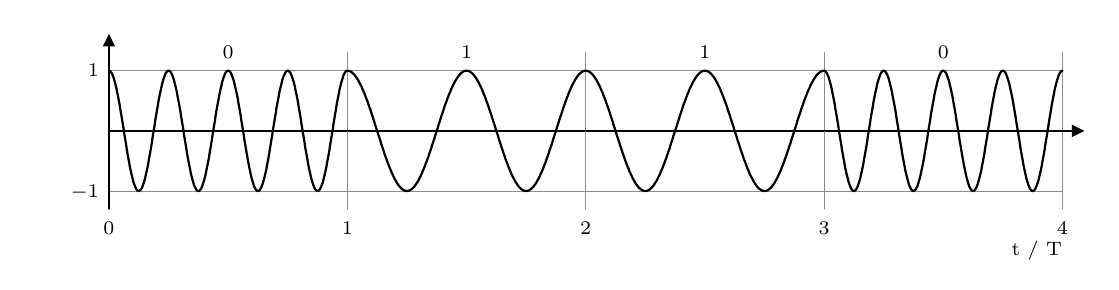
\begin{tikzpicture}[x=0.01985cm,y=-0.01985cm,line cap=round,line join=round]
\useasboundingbox (0,0) rectangle (680,150);
\path[draw=black!45,line width=0.35pt] (52,116) -- (52,16);
\path[draw=black!45,line width=0.35pt] (204.5,116) -- (204.5,16);
\path[draw=black!45,line width=0.35pt] (357,116) -- (357,16);
\path[draw=black!45,line width=0.35pt] (509.5,116) -- (509.5,16);
\path[draw=black!45,line width=0.35pt] (662,116) -- (662,16);
\path[draw=black!45,line width=0.35pt] (52,27.5) -- (662,27.5);
\path[draw=black!45,line width=0.35pt] (52,104.5) -- (662,104.5);
\path[draw=black,line width=0.7pt] (52,66) -- (670,66);
\path[fill=black,draw=none] (676,66) -- (668,62) -- (668,70) -- cycle;
\path[draw=black,line width=0.7pt] (52,116) -- (52,10);
\path[fill=black,draw=none] (52,4) -- (48,12) -- (56,12) -- cycle;
\node[anchor=base,inner sep=0pt,font=\scriptsize] at (52,132) {0};
\node[anchor=base,inner sep=0pt,font=\scriptsize] at (204.5,132) {1};
\node[anchor=base,inner sep=0pt,font=\scriptsize] at (357,132) {2};
\node[anchor=base,inner sep=0pt,font=\scriptsize] at (509.5,132) {3};
\node[anchor=base,inner sep=0pt,font=\scriptsize] at (662,132) {4};
\node[anchor=base east,inner sep=0pt,font=\scriptsize] at (46,31.5) {1};
\node[anchor=base east,inner sep=0pt,font=\scriptsize] at (46,108.5) {$-$1};
\node[anchor=base east,inner sep=0pt,font=\scriptsize] at (662,146) {t / T};
\path[draw=black!45,line width=0.35pt,dash pattern=on 3pt off 2pt] (204.5,116) -- (204.5,16);
\path[draw=black!45,line width=0.35pt,dash pattern=on 3pt off 2pt] (357,116) -- (357,16);
\path[draw=black!45,line width=0.35pt,dash pattern=on 3pt off 2pt] (509.5,116) -- (509.5,16);
\path[draw=black,line width=0.8pt] (52,27.5) -- (52.4,27.6) -- (52.8,27.8) -- (53.1,28.2) -- (53.5,28.7) -- (53.9,29.4) -- (54.3,30.2) -- (54.7,31.2) -- (55.1,32.3) -- (55.4,33.5) -- (55.8,34.9) -- (56.2,36.4) -- (56.6,38) -- (57,39.7) -- (57.3,41.5) -- (57.7,43.4) -- (58.1,45.4) -- (58.5,47.5) -- (58.9,49.6) -- (59.2,51.8) -- (59.6,54.1) -- (60,56.4) -- (60.4,58.8) -- (60.8,61.2) -- (61.2,63.6) -- (61.5,66) -- (61.9,68.4) -- (62.3,70.8) -- (62.7,73.2) -- (63.1,75.6) -- (63.4,77.9) -- (63.8,80.2) -- (64.2,82.4) -- (64.6,84.5) -- (65,86.6) -- (65.3,88.6) -- (65.7,90.5) -- (66.1,92.3) -- (66.5,94) -- (66.9,95.6) -- (67.3,97.1) -- (67.6,98.5) -- (68,99.7) -- (68.4,100.8) -- (68.8,101.8) -- (69.2,102.6) -- (69.5,103.3) -- (69.9,103.8) -- (70.3,104.2) -- (70.7,104.4) -- (71.1,104.5) -- (71.4,104.4) -- (71.8,104.2) -- (72.2,103.8) -- (72.6,103.3) -- (73,102.6) -- (73.4,101.8) -- (73.7,100.8) -- (74.1,99.7) -- (74.5,98.5) -- (74.9,97.1) -- (75.3,95.6) -- (75.6,94) -- (76,92.3) -- (76.4,90.5) -- (76.8,88.6) -- (77.2,86.6) -- (77.5,84.5) -- (77.9,82.4) -- (78.3,80.2) -- (78.7,77.9) -- (79.1,75.6) -- (79.5,73.2) -- (79.8,70.8) -- (80.2,68.4) -- (80.6,66) -- (81,63.6) -- (81.4,61.2) -- (81.7,58.8) -- (82.1,56.4) -- (82.5,54.1) -- (82.9,51.8) -- (83.3,49.6) -- (83.6,47.5) -- (84,45.4) -- (84.4,43.4) -- (84.8,41.5) -- (85.2,39.7) -- (85.6,38) -- (85.9,36.4) -- (86.3,34.9) -- (86.7,33.5) -- (87.1,32.3) -- (87.5,31.2) -- (87.8,30.2) -- (88.2,29.4) -- (88.6,28.7) -- (89,28.2) -- (89.4,27.8) -- (89.7,27.6) -- (90.1,27.5) -- (90.5,27.6) -- (90.9,27.8) -- (91.3,28.2) -- (91.7,28.7) -- (92,29.4) -- (92.4,30.2) -- (92.8,31.2) -- (93.2,32.3) -- (93.6,33.5) -- (93.9,34.9) -- (94.3,36.4) -- (94.7,38) -- (95.1,39.7) -- (95.5,41.5) -- (95.8,43.4) -- (96.2,45.4) -- (96.6,47.5) -- (97,49.6) -- (97.4,51.8) -- (97.8,54.1) -- (98.1,56.4) -- (98.5,58.8) -- (98.9,61.2) -- (99.3,63.6) -- (99.7,66) -- (100,68.4) -- (100.4,70.8) -- (100.8,73.2) -- (101.2,75.6) -- (101.6,77.9) -- (101.9,80.2) -- (102.3,82.4) -- (102.7,84.5) -- (103.1,86.6) -- (103.5,88.6) -- (103.9,90.5) -- (104.2,92.3) -- (104.6,94) -- (105,95.6) -- (105.4,97.1) -- (105.8,98.5) -- (106.1,99.7) -- (106.5,100.8) -- (106.9,101.8) -- (107.3,102.6) -- (107.7,103.3) -- (108,103.8) -- (108.4,104.2) -- (108.8,104.4) -- (109.2,104.5) -- (109.6,104.4) -- (110,104.2) -- (110.3,103.8) -- (110.7,103.3) -- (111.1,102.6) -- (111.5,101.8) -- (111.9,100.8) -- (112.2,99.7) -- (112.6,98.5) -- (113,97.1) -- (113.4,95.6) -- (113.8,94) -- (114.1,92.3) -- (114.5,90.5) -- (114.9,88.6) -- (115.3,86.6) -- (115.7,84.5) -- (116.1,82.4) -- (116.4,80.2) -- (116.8,77.9) -- (117.2,75.6) -- (117.6,73.2) -- (118,70.8) -- (118.3,68.4) -- (118.7,66) -- (119.1,63.6) -- (119.5,61.2) -- (119.9,58.8) -- (120.2,56.4) -- (120.6,54.1) -- (121,51.8) -- (121.4,49.6) -- (121.8,47.5) -- (122.2,45.4) -- (122.5,43.4) -- (122.9,41.5) -- (123.3,39.7) -- (123.7,38) -- (124.1,36.4) -- (124.4,34.9) -- (124.8,33.5) -- (125.2,32.3) -- (125.6,31.2) -- (126,30.2) -- (126.3,29.4) -- (126.7,28.7) -- (127.1,28.2) -- (127.5,27.8) -- (127.9,27.6) -- (128.3,27.5) -- (128.6,27.6) -- (129,27.8) -- (129.4,28.2) -- (129.8,28.7) -- (130.2,29.4) -- (130.5,30.2) -- (130.9,31.2) -- (131.3,32.3) -- (131.7,33.5) -- (132.1,34.9) -- (132.4,36.4) -- (132.8,38) -- (133.2,39.7) -- (133.6,41.5) -- (134,43.4) -- (134.4,45.4) -- (134.7,47.5) -- (135.1,49.6) -- (135.5,51.8) -- (135.9,54.1) -- (136.3,56.4) -- (136.6,58.8) -- (137,61.2) -- (137.4,63.6) -- (137.8,66) -- (138.2,68.4) -- (138.5,70.8) -- (138.9,73.2) -- (139.3,75.6) -- (139.7,77.9) -- (140.1,80.2) -- (140.5,82.4) -- (140.8,84.5) -- (141.2,86.6) -- (141.6,88.6) -- (142,90.5) -- (142.4,92.3) -- (142.7,94) -- (143.1,95.6) -- (143.5,97.1) -- (143.9,98.5) -- (144.3,99.7) -- (144.6,100.8) -- (145,101.8) -- (145.4,102.6) -- (145.8,103.3) -- (146.2,103.8) -- (146.6,104.2) -- (146.9,104.4) -- (147.3,104.5) -- (147.7,104.4) -- (148.1,104.2) -- (148.5,103.8) -- (148.8,103.3) -- (149.2,102.6) -- (149.6,101.8) -- (150,100.8) -- (150.4,99.7) -- (150.7,98.5) -- (151.1,97.1) -- (151.5,95.6) -- (151.9,94) -- (152.3,92.3) -- (152.7,90.5) -- (153,88.6) -- (153.4,86.6) -- (153.8,84.5) -- (154.2,82.4) -- (154.6,80.2) -- (154.9,77.9) -- (155.3,75.6) -- (155.7,73.2) -- (156.1,70.8) -- (156.5,68.4) -- (156.8,66) -- (157.2,63.6) -- (157.6,61.2) -- (158,58.8) -- (158.4,56.4) -- (158.8,54.1) -- (159.1,51.8) -- (159.5,49.6) -- (159.9,47.5) -- (160.3,45.4) -- (160.7,43.4) -- (161,41.5) -- (161.4,39.7) -- (161.8,38) -- (162.2,36.4) -- (162.6,34.9) -- (162.9,33.5) -- (163.3,32.3) -- (163.7,31.2) -- (164.1,30.2) -- (164.5,29.4) -- (164.9,28.7) -- (165.2,28.2) -- (165.6,27.8) -- (166,27.6) -- (166.4,27.5) -- (166.8,27.6) -- (167.1,27.8) -- (167.5,28.2) -- (167.9,28.7) -- (168.3,29.4) -- (168.7,30.2) -- (169,31.2) -- (169.4,32.3) -- (169.8,33.5) -- (170.2,34.9) -- (170.6,36.4) -- (171,38) -- (171.3,39.7) -- (171.7,41.5) -- (172.1,43.4) -- (172.5,45.4) -- (172.9,47.5) -- (173.2,49.6) -- (173.6,51.8) -- (174,54.1) -- (174.4,56.4) -- (174.8,58.8) -- (175.1,61.2) -- (175.5,63.6) -- (175.9,66) -- (176.3,68.4) -- (176.7,70.8) -- (177.1,73.2) -- (177.4,75.6) -- (177.8,77.9) -- (178.2,80.2) -- (178.6,82.4) -- (179,84.5) -- (179.3,86.6) -- (179.7,88.6) -- (180.1,90.5) -- (180.5,92.3) -- (180.9,94) -- (181.2,95.6) -- (181.6,97.1) -- (182,98.5) -- (182.4,99.7) -- (182.8,100.8) -- (183.2,101.8) -- (183.5,102.6) -- (183.9,103.3) -- (184.3,103.8) -- (184.7,104.2) -- (185.1,104.4) -- (185.4,104.5) -- (185.8,104.4) -- (186.2,104.2) -- (186.6,103.8) -- (187,103.3) -- (187.3,102.6) -- (187.7,101.8) -- (188.1,100.8) -- (188.5,99.7) -- (188.9,98.5) -- (189.3,97.1) -- (189.6,95.6) -- (190,94) -- (190.4,92.3) -- (190.8,90.5) -- (191.2,88.6) -- (191.5,86.6) -- (191.9,84.5) -- (192.3,82.4) -- (192.7,80.2) -- (193.1,77.9) -- (193.4,75.6) -- (193.8,73.2) -- (194.2,70.8) -- (194.6,68.4) -- (195,66) -- (195.4,63.6) -- (195.7,61.2) -- (196.1,58.8) -- (196.5,56.4) -- (196.9,54.1) -- (197.3,51.8) -- (197.6,49.6) -- (198,47.5) -- (198.4,45.4) -- (198.8,43.4) -- (199.2,41.5) -- (199.5,39.7) -- (199.9,38) -- (200.3,36.4) -- (200.7,34.9) -- (201.1,33.5) -- (201.5,32.3) -- (201.8,31.2) -- (202.2,30.2) -- (202.6,29.4) -- (203,28.7) -- (203.4,28.2) -- (203.7,27.8) -- (204.1,27.6) -- (204.5,27.5) -- (204.9,27.6) -- (205.3,27.6) -- (205.6,27.7) -- (206,27.8) -- (206.4,28) -- (206.8,28.2) -- (207.2,28.5) -- (207.6,28.7) -- (207.9,29.1) -- (208.3,29.4) -- (208.7,29.8) -- (209.1,30.2) -- (209.5,30.7) -- (209.8,31.2) -- (210.2,31.7) -- (210.6,32.3) -- (211,32.9) -- (211.4,33.5) -- (211.7,34.2) -- (212.1,34.9) -- (212.5,35.6) -- (212.9,36.4) -- (213.3,37.1) -- (213.7,38) -- (214,38.8) -- (214.4,39.7) -- (214.8,40.6) -- (215.2,41.5) -- (215.6,42.4) -- (215.9,43.4) -- (216.3,44.4) -- (216.7,45.4) -- (217.1,46.4) -- (217.5,47.5) -- (217.8,48.5) -- (218.2,49.6) -- (218.6,50.7) -- (219,51.8) -- (219.4,53) -- (219.8,54.1) -- (220.1,55.3) -- (220.5,56.4) -- (220.9,57.6) -- (221.3,58.8) -- (221.7,60) -- (222,61.2) -- (222.4,62.4) -- (222.8,63.6) -- (223.2,64.8) -- (223.6,66) -- (223.9,67.2) -- (224.3,68.4) -- (224.7,69.6) -- (225.1,70.8) -- (225.5,72) -- (225.9,73.2) -- (226.2,74.4) -- (226.6,75.6) -- (227,76.7) -- (227.4,77.9) -- (227.8,79) -- (228.1,80.2) -- (228.5,81.3) -- (228.9,82.4) -- (229.3,83.5) -- (229.7,84.5) -- (230,85.6) -- (230.4,86.6) -- (230.8,87.6) -- (231.2,88.6) -- (231.6,89.6) -- (232,90.5) -- (232.3,91.4) -- (232.7,92.3) -- (233.1,93.2) -- (233.5,94) -- (233.9,94.9) -- (234.2,95.6) -- (234.6,96.4) -- (235,97.1) -- (235.4,97.8) -- (235.8,98.5) -- (236.1,99.1) -- (236.5,99.7) -- (236.9,100.3) -- (237.3,100.8) -- (237.7,101.3) -- (238.1,101.8) -- (238.4,102.2) -- (238.8,102.6) -- (239.2,102.9) -- (239.6,103.3) -- (240,103.5) -- (240.3,103.8) -- (240.7,104) -- (241.1,104.2) -- (241.5,104.3) -- (241.9,104.4) -- (242.2,104.4) -- (242.6,104.5) -- (243,104.4) -- (243.4,104.4) -- (243.8,104.3) -- (244.2,104.2) -- (244.5,104) -- (244.9,103.8) -- (245.3,103.5) -- (245.7,103.3) -- (246.1,102.9) -- (246.4,102.6) -- (246.8,102.2) -- (247.2,101.8) -- (247.6,101.3) -- (248,100.8) -- (248.3,100.3) -- (248.7,99.7) -- (249.1,99.1) -- (249.5,98.5) -- (249.9,97.8) -- (250.3,97.1) -- (250.6,96.4) -- (251,95.6) -- (251.4,94.9) -- (251.8,94) -- (252.2,93.2) -- (252.5,92.3) -- (252.9,91.4) -- (253.3,90.5) -- (253.7,89.6) -- (254.1,88.6) -- (254.4,87.6) -- (254.8,86.6) -- (255.2,85.6) -- (255.6,84.5) -- (256,83.5) -- (256.4,82.4) -- (256.7,81.3) -- (257.1,80.2) -- (257.5,79) -- (257.9,77.9) -- (258.3,76.7) -- (258.6,75.6) -- (259,74.4) -- (259.4,73.2) -- (259.8,72) -- (260.2,70.8) -- (260.5,69.6) -- (260.9,68.4) -- (261.3,67.2) -- (261.7,66) -- (262.1,64.8) -- (262.5,63.6) -- (262.8,62.4) -- (263.2,61.2) -- (263.6,60) -- (264,58.8) -- (264.4,57.6) -- (264.7,56.4) -- (265.1,55.3) -- (265.5,54.1) -- (265.9,53) -- (266.3,51.8) -- (266.6,50.7) -- (267,49.6) -- (267.4,48.5) -- (267.8,47.5) -- (268.2,46.4) -- (268.5,45.4) -- (268.9,44.4) -- (269.3,43.4) -- (269.7,42.4) -- (270.1,41.5) -- (270.5,40.6) -- (270.8,39.7) -- (271.2,38.8) -- (271.6,38) -- (272,37.1) -- (272.4,36.4) -- (272.7,35.6) -- (273.1,34.9) -- (273.5,34.2) -- (273.9,33.5) -- (274.3,32.9) -- (274.7,32.3) -- (275,31.7) -- (275.4,31.2) -- (275.8,30.7) -- (276.2,30.2) -- (276.6,29.8) -- (276.9,29.4) -- (277.3,29.1) -- (277.7,28.7) -- (278.1,28.5) -- (278.5,28.2) -- (278.8,28) -- (279.2,27.8) -- (279.6,27.7) -- (280,27.6) -- (280.4,27.6) -- (280.8,27.5) -- (281.1,27.6) -- (281.5,27.6) -- (281.9,27.7) -- (282.3,27.8) -- (282.7,28) -- (283,28.2) -- (283.4,28.5) -- (283.8,28.7) -- (284.2,29.1) -- (284.6,29.4) -- (284.9,29.8) -- (285.3,30.2) -- (285.7,30.7) -- (286.1,31.2) -- (286.5,31.7) -- (286.9,32.3) -- (287.2,32.9) -- (287.6,33.5) -- (288,34.2) -- (288.4,34.9) -- (288.8,35.6) -- (289.1,36.4) -- (289.5,37.1) -- (289.9,38) -- (290.3,38.8) -- (290.7,39.7) -- (291,40.6) -- (291.4,41.5) -- (291.8,42.4) -- (292.2,43.4) -- (292.6,44.4) -- (293,45.4) -- (293.3,46.4) -- (293.7,47.5) -- (294.1,48.5) -- (294.5,49.6) -- (294.9,50.7) -- (295.2,51.8) -- (295.6,53) -- (296,54.1) -- (296.4,55.3) -- (296.8,56.4) -- (297.1,57.6) -- (297.5,58.8) -- (297.9,60) -- (298.3,61.2) -- (298.7,62.4) -- (299.1,63.6) -- (299.4,64.8) -- (299.8,66) -- (300.2,67.2) -- (300.6,68.4) -- (301,69.6) -- (301.3,70.8) -- (301.7,72) -- (302.1,73.2) -- (302.5,74.4) -- (302.9,75.6) -- (303.2,76.7) -- (303.6,77.9) -- (304,79) -- (304.4,80.2) -- (304.8,81.3) -- (305.2,82.4) -- (305.5,83.5) -- (305.9,84.5) -- (306.3,85.6) -- (306.7,86.6) -- (307.1,87.6) -- (307.4,88.6) -- (307.8,89.6) -- (308.2,90.5) -- (308.6,91.4) -- (309,92.3) -- (309.3,93.2) -- (309.7,94) -- (310.1,94.9) -- (310.5,95.6) -- (310.9,96.4) -- (311.3,97.1) -- (311.6,97.8) -- (312,98.5) -- (312.4,99.1) -- (312.8,99.7) -- (313.2,100.3) -- (313.5,100.8) -- (313.9,101.3) -- (314.3,101.8) -- (314.7,102.2) -- (315.1,102.6) -- (315.4,102.9) -- (315.8,103.3) -- (316.2,103.5) -- (316.6,103.8) -- (317,104) -- (317.4,104.2) -- (317.7,104.3) -- (318.1,104.4) -- (318.5,104.4) -- (318.9,104.5) -- (319.3,104.4) -- (319.6,104.4) -- (320,104.3) -- (320.4,104.2) -- (320.8,104) -- (321.2,103.8) -- (321.5,103.5) -- (321.9,103.3) -- (322.3,102.9) -- (322.7,102.6) -- (323.1,102.2) -- (323.5,101.8) -- (323.8,101.3) -- (324.2,100.8) -- (324.6,100.3) -- (325,99.7) -- (325.4,99.1) -- (325.7,98.5) -- (326.1,97.8) -- (326.5,97.1) -- (326.9,96.4) -- (327.3,95.6) -- (327.6,94.9) -- (328,94) -- (328.4,93.2) -- (328.8,92.3) -- (329.2,91.4) -- (329.6,90.5) -- (329.9,89.6) -- (330.3,88.6) -- (330.7,87.6) -- (331.1,86.6) -- (331.5,85.6) -- (331.8,84.5) -- (332.2,83.5) -- (332.6,82.4) -- (333,81.3) -- (333.4,80.2) -- (333.7,79) -- (334.1,77.9) -- (334.5,76.7) -- (334.9,75.6) -- (335.3,74.4) -- (335.7,73.2) -- (336,72) -- (336.4,70.8) -- (336.8,69.6) -- (337.2,68.4) -- (337.6,67.2) -- (337.9,66) -- (338.3,64.8) -- (338.7,63.6) -- (339.1,62.4) -- (339.5,61.2) -- (339.8,60) -- (340.2,58.8) -- (340.6,57.6) -- (341,56.4) -- (341.4,55.3) -- (341.8,54.1) -- (342.1,53) -- (342.5,51.8) -- (342.9,50.7) -- (343.3,49.6) -- (343.7,48.5) -- (344,47.5) -- (344.4,46.4) -- (344.8,45.4) -- (345.2,44.4) -- (345.6,43.4) -- (345.9,42.4) -- (346.3,41.5) -- (346.7,40.6) -- (347.1,39.7) -- (347.5,38.8) -- (347.8,38) -- (348.2,37.1) -- (348.6,36.4) -- (349,35.6) -- (349.4,34.9) -- (349.8,34.2) -- (350.1,33.5) -- (350.5,32.9) -- (350.9,32.3) -- (351.3,31.7) -- (351.7,31.2) -- (352,30.7) -- (352.4,30.2) -- (352.8,29.8) -- (353.2,29.4) -- (353.6,29.1) -- (354,28.7) -- (354.3,28.5) -- (354.7,28.2) -- (355.1,28) -- (355.5,27.8) -- (355.9,27.7) -- (356.2,27.6) -- (356.6,27.6) -- (357,27.5) -- (357.4,27.6) -- (357.8,27.6) -- (358.1,27.7) -- (358.5,27.8) -- (358.9,28) -- (359.3,28.2) -- (359.7,28.5) -- (360.1,28.7) -- (360.4,29.1) -- (360.8,29.4) -- (361.2,29.8) -- (361.6,30.2) -- (362,30.7) -- (362.3,31.2) -- (362.7,31.7) -- (363.1,32.3) -- (363.5,32.9) -- (363.9,33.5) -- (364.2,34.2) -- (364.6,34.9) -- (365,35.6) -- (365.4,36.4) -- (365.8,37.1) -- (366.2,38) -- (366.5,38.8) -- (366.9,39.7) -- (367.3,40.6) -- (367.7,41.5) -- (368.1,42.4) -- (368.4,43.4) -- (368.8,44.4) -- (369.2,45.4) -- (369.6,46.4) -- (370,47.5) -- (370.3,48.5) -- (370.7,49.6) -- (371.1,50.7) -- (371.5,51.8) -- (371.9,53) -- (372.3,54.1) -- (372.6,55.3) -- (373,56.4) -- (373.4,57.6) -- (373.8,58.8) -- (374.2,60) -- (374.5,61.2) -- (374.9,62.4) -- (375.3,63.6) -- (375.7,64.8) -- (376.1,66) -- (376.4,67.2) -- (376.8,68.4) -- (377.2,69.6) -- (377.6,70.8) -- (378,72) -- (378.4,73.2) -- (378.7,74.4) -- (379.1,75.6) -- (379.5,76.7) -- (379.9,77.9) -- (380.3,79) -- (380.6,80.2) -- (381,81.3) -- (381.4,82.4) -- (381.8,83.5) -- (382.2,84.5) -- (382.5,85.6) -- (382.9,86.6) -- (383.3,87.6) -- (383.7,88.6) -- (384.1,89.6) -- (384.5,90.5) -- (384.8,91.4) -- (385.2,92.3) -- (385.6,93.2) -- (386,94) -- (386.4,94.9) -- (386.7,95.6) -- (387.1,96.4) -- (387.5,97.1) -- (387.9,97.8) -- (388.3,98.5) -- (388.6,99.1) -- (389,99.7) -- (389.4,100.3) -- (389.8,100.8) -- (390.2,101.3) -- (390.6,101.8) -- (390.9,102.2) -- (391.3,102.6) -- (391.7,102.9) -- (392.1,103.3) -- (392.5,103.5) -- (392.8,103.8) -- (393.2,104) -- (393.6,104.2) -- (394,104.3) -- (394.4,104.4) -- (394.7,104.4) -- (395.1,104.5) -- (395.5,104.4) -- (395.9,104.4) -- (396.3,104.3) -- (396.7,104.2) -- (397,104) -- (397.4,103.8) -- (397.8,103.5) -- (398.2,103.3) -- (398.6,102.9) -- (398.9,102.6) -- (399.3,102.2) -- (399.7,101.8) -- (400.1,101.3) -- (400.5,100.8) -- (400.8,100.3) -- (401.2,99.7) -- (401.6,99.1) -- (402,98.5) -- (402.4,97.8) -- (402.8,97.1) -- (403.1,96.4) -- (403.5,95.6) -- (403.9,94.9) -- (404.3,94) -- (404.7,93.2) -- (405,92.3) -- (405.4,91.4) -- (405.8,90.5) -- (406.2,89.6) -- (406.6,88.6) -- (406.9,87.6) -- (407.3,86.6) -- (407.7,85.6) -- (408.1,84.5) -- (408.5,83.5) -- (408.8,82.4) -- (409.2,81.3) -- (409.6,80.2) -- (410,79) -- (410.4,77.9) -- (410.8,76.7) -- (411.1,75.6) -- (411.5,74.4) -- (411.9,73.2) -- (412.3,72) -- (412.7,70.8) -- (413,69.6) -- (413.4,68.4) -- (413.8,67.2) -- (414.2,66) -- (414.6,64.8) -- (415,63.6) -- (415.3,62.4) -- (415.7,61.2) -- (416.1,60) -- (416.5,58.8) -- (416.9,57.6) -- (417.2,56.4) -- (417.6,55.3) -- (418,54.1) -- (418.4,53) -- (418.8,51.8) -- (419.1,50.7) -- (419.5,49.6) -- (419.9,48.5) -- (420.3,47.5) -- (420.7,46.4) -- (421.1,45.4) -- (421.4,44.4) -- (421.8,43.4) -- (422.2,42.4) -- (422.6,41.5) -- (423,40.6) -- (423.3,39.7) -- (423.7,38.8) -- (424.1,38) -- (424.5,37.1) -- (424.9,36.4) -- (425.2,35.6) -- (425.6,34.9) -- (426,34.2) -- (426.4,33.5) -- (426.8,32.9) -- (427.2,32.3) -- (427.5,31.7) -- (427.9,31.2) -- (428.3,30.7) -- (428.7,30.2) -- (429.1,29.8) -- (429.4,29.4) -- (429.8,29.1) -- (430.2,28.7) -- (430.6,28.5) -- (431,28.2) -- (431.3,28) -- (431.7,27.8) -- (432.1,27.7) -- (432.5,27.6) -- (432.9,27.6) -- (433.3,27.5) -- (433.6,27.6) -- (434,27.6) -- (434.4,27.7) -- (434.8,27.8) -- (435.2,28) -- (435.5,28.2) -- (435.9,28.5) -- (436.3,28.7) -- (436.7,29.1) -- (437.1,29.4) -- (437.4,29.8) -- (437.8,30.2) -- (438.2,30.7) -- (438.6,31.2) -- (439,31.7) -- (439.4,32.3) -- (439.7,32.9) -- (440.1,33.5) -- (440.5,34.2) -- (440.9,34.9) -- (441.3,35.6) -- (441.6,36.4) -- (442,37.1) -- (442.4,38) -- (442.8,38.8) -- (443.2,39.7) -- (443.5,40.6) -- (443.9,41.5) -- (444.3,42.4) -- (444.7,43.4) -- (445.1,44.4) -- (445.5,45.4) -- (445.8,46.4) -- (446.2,47.5) -- (446.6,48.5) -- (447,49.6) -- (447.4,50.7) -- (447.7,51.8) -- (448.1,53) -- (448.5,54.1) -- (448.9,55.3) -- (449.3,56.4) -- (449.6,57.6) -- (450,58.8) -- (450.4,60) -- (450.8,61.2) -- (451.2,62.4) -- (451.6,63.6) -- (451.9,64.8) -- (452.3,66) -- (452.7,67.2) -- (453.1,68.4) -- (453.5,69.6) -- (453.8,70.8) -- (454.2,72) -- (454.6,73.2) -- (455,74.4) -- (455.4,75.6) -- (455.7,76.7) -- (456.1,77.9) -- (456.5,79) -- (456.9,80.2) -- (457.3,81.3) -- (457.7,82.4) -- (458,83.5) -- (458.4,84.5) -- (458.8,85.6) -- (459.2,86.6) -- (459.6,87.6) -- (459.9,88.6) -- (460.3,89.6) -- (460.7,90.5) -- (461.1,91.4) -- (461.5,92.3) -- (461.8,93.2) -- (462.2,94) -- (462.6,94.9) -- (463,95.6) -- (463.4,96.4) -- (463.8,97.1) -- (464.1,97.8) -- (464.5,98.5) -- (464.9,99.1) -- (465.3,99.7) -- (465.7,100.3) -- (466,100.8) -- (466.4,101.3) -- (466.8,101.8) -- (467.2,102.2) -- (467.6,102.6) -- (467.9,102.9) -- (468.3,103.3) -- (468.7,103.5) -- (469.1,103.8) -- (469.5,104) -- (469.9,104.2) -- (470.2,104.3) -- (470.6,104.4) -- (471,104.4) -- (471.4,104.5) -- (471.8,104.4) -- (472.1,104.4) -- (472.5,104.3) -- (472.9,104.2) -- (473.3,104) -- (473.7,103.8) -- (474,103.5) -- (474.4,103.3) -- (474.8,102.9) -- (475.2,102.6) -- (475.6,102.2) -- (476,101.8) -- (476.3,101.3) -- (476.7,100.8) -- (477.1,100.3) -- (477.5,99.7) -- (477.9,99.1) -- (478.2,98.5) -- (478.6,97.8) -- (479,97.1) -- (479.4,96.4) -- (479.8,95.6) -- (480.1,94.9) -- (480.5,94) -- (480.9,93.2) -- (481.3,92.3) -- (481.7,91.4) -- (482.1,90.5) -- (482.4,89.6) -- (482.8,88.6) -- (483.2,87.6) -- (483.6,86.6) -- (484,85.6) -- (484.3,84.5) -- (484.7,83.5) -- (485.1,82.4) -- (485.5,81.3) -- (485.9,80.2) -- (486.2,79) -- (486.6,77.9) -- (487,76.7) -- (487.4,75.6) -- (487.8,74.4) -- (488.2,73.2) -- (488.5,72) -- (488.9,70.8) -- (489.3,69.6) -- (489.7,68.4) -- (490.1,67.2) -- (490.4,66) -- (490.8,64.8) -- (491.2,63.6) -- (491.6,62.4) -- (492,61.2) -- (492.3,60) -- (492.7,58.8) -- (493.1,57.6) -- (493.5,56.4) -- (493.9,55.3) -- (494.3,54.1) -- (494.6,53) -- (495,51.8) -- (495.4,50.7) -- (495.8,49.6) -- (496.2,48.5) -- (496.5,47.5) -- (496.9,46.4) -- (497.3,45.4) -- (497.7,44.4) -- (498.1,43.4) -- (498.4,42.4) -- (498.8,41.5) -- (499.2,40.6) -- (499.6,39.7) -- (500,38.8) -- (500.4,38) -- (500.7,37.1) -- (501.1,36.4) -- (501.5,35.6) -- (501.9,34.9) -- (502.3,34.2) -- (502.6,33.5) -- (503,32.9) -- (503.4,32.3) -- (503.8,31.7) -- (504.2,31.2) -- (504.5,30.7) -- (504.9,30.2) -- (505.3,29.8) -- (505.7,29.4) -- (506.1,29.1) -- (506.5,28.7) -- (506.8,28.5) -- (507.2,28.2) -- (507.6,28) -- (508,27.8) -- (508.4,27.7) -- (508.7,27.6) -- (509.1,27.6) -- (509.5,27.5) -- (509.9,27.6) -- (510.3,27.8) -- (510.6,28.2) -- (511,28.7) -- (511.4,29.4) -- (511.8,30.2) -- (512.2,31.2) -- (512.6,32.3) -- (512.9,33.5) -- (513.3,34.9) -- (513.7,36.4) -- (514.1,38) -- (514.5,39.7) -- (514.8,41.5) -- (515.2,43.4) -- (515.6,45.4) -- (516,47.5) -- (516.4,49.6) -- (516.7,51.8) -- (517.1,54.1) -- (517.5,56.4) -- (517.9,58.8) -- (518.3,61.2) -- (518.7,63.6) -- (519,66) -- (519.4,68.4) -- (519.8,70.8) -- (520.2,73.2) -- (520.6,75.6) -- (520.9,77.9) -- (521.3,80.2) -- (521.7,82.4) -- (522.1,84.5) -- (522.5,86.6) -- (522.8,88.6) -- (523.2,90.5) -- (523.6,92.3) -- (524,94) -- (524.4,95.6) -- (524.8,97.1) -- (525.1,98.5) -- (525.5,99.7) -- (525.9,100.8) -- (526.3,101.8) -- (526.7,102.6) -- (527,103.3) -- (527.4,103.8) -- (527.8,104.2) -- (528.2,104.4) -- (528.6,104.5) -- (528.9,104.4) -- (529.3,104.2) -- (529.7,103.8) -- (530.1,103.3) -- (530.5,102.6) -- (530.9,101.8) -- (531.2,100.8) -- (531.6,99.7) -- (532,98.5) -- (532.4,97.1) -- (532.8,95.6) -- (533.1,94) -- (533.5,92.3) -- (533.9,90.5) -- (534.3,88.6) -- (534.7,86.6) -- (535,84.5) -- (535.4,82.4) -- (535.8,80.2) -- (536.2,77.9) -- (536.6,75.6) -- (537,73.2) -- (537.3,70.8) -- (537.7,68.4) -- (538.1,66) -- (538.5,63.6) -- (538.9,61.2) -- (539.2,58.8) -- (539.6,56.4) -- (540,54.1) -- (540.4,51.8) -- (540.8,49.6) -- (541.1,47.5) -- (541.5,45.4) -- (541.9,43.4) -- (542.3,41.5) -- (542.7,39.7) -- (543.1,38) -- (543.4,36.4) -- (543.8,34.9) -- (544.2,33.5) -- (544.6,32.3) -- (545,31.2) -- (545.3,30.2) -- (545.7,29.4) -- (546.1,28.7) -- (546.5,28.2) -- (546.9,27.8) -- (547.2,27.6) -- (547.6,27.5) -- (548,27.6) -- (548.4,27.8) -- (548.8,28.2) -- (549.2,28.7) -- (549.5,29.4) -- (549.9,30.2) -- (550.3,31.2) -- (550.7,32.3) -- (551.1,33.5) -- (551.4,34.9) -- (551.8,36.4) -- (552.2,38) -- (552.6,39.7) -- (553,41.5) -- (553.3,43.4) -- (553.7,45.4) -- (554.1,47.5) -- (554.5,49.6) -- (554.9,51.8) -- (555.3,54.1) -- (555.6,56.4) -- (556,58.8) -- (556.4,61.2) -- (556.8,63.6) -- (557.2,66) -- (557.5,68.4) -- (557.9,70.8) -- (558.3,73.2) -- (558.7,75.6) -- (559.1,77.9) -- (559.4,80.2) -- (559.8,82.4) -- (560.2,84.5) -- (560.6,86.6) -- (561,88.6) -- (561.3,90.5) -- (561.7,92.3) -- (562.1,94) -- (562.5,95.6) -- (562.9,97.1) -- (563.3,98.5) -- (563.6,99.7) -- (564,100.8) -- (564.4,101.8) -- (564.8,102.6) -- (565.2,103.3) -- (565.5,103.8) -- (565.9,104.2) -- (566.3,104.4) -- (566.7,104.5) -- (567.1,104.4) -- (567.4,104.2) -- (567.8,103.8) -- (568.2,103.3) -- (568.6,102.6) -- (569,101.8) -- (569.4,100.8) -- (569.7,99.7) -- (570.1,98.5) -- (570.5,97.1) -- (570.9,95.6) -- (571.3,94) -- (571.6,92.3) -- (572,90.5) -- (572.4,88.6) -- (572.8,86.6) -- (573.2,84.5) -- (573.6,82.4) -- (573.9,80.2) -- (574.3,77.9) -- (574.7,75.6) -- (575.1,73.2) -- (575.5,70.8) -- (575.8,68.4) -- (576.2,66) -- (576.6,63.6) -- (577,61.2) -- (577.4,58.8) -- (577.7,56.4) -- (578.1,54.1) -- (578.5,51.8) -- (578.9,49.6) -- (579.3,47.5) -- (579.7,45.4) -- (580,43.4) -- (580.4,41.5) -- (580.8,39.7) -- (581.2,38) -- (581.6,36.4) -- (581.9,34.9) -- (582.3,33.5) -- (582.7,32.3) -- (583.1,31.2) -- (583.5,30.2) -- (583.8,29.4) -- (584.2,28.7) -- (584.6,28.2) -- (585,27.8) -- (585.4,27.6) -- (585.8,27.5) -- (586.1,27.6) -- (586.5,27.8) -- (586.9,28.2) -- (587.3,28.7) -- (587.7,29.4) -- (588,30.2) -- (588.4,31.2) -- (588.8,32.3) -- (589.2,33.5) -- (589.6,34.9) -- (589.9,36.4) -- (590.3,38) -- (590.7,39.7) -- (591.1,41.5) -- (591.5,43.4) -- (591.9,45.4) -- (592.2,47.5) -- (592.6,49.6) -- (593,51.8) -- (593.4,54.1) -- (593.8,56.4) -- (594.1,58.8) -- (594.5,61.2) -- (594.9,63.6) -- (595.3,66) -- (595.7,68.4) -- (596,70.8) -- (596.4,73.2) -- (596.8,75.6) -- (597.2,77.9) -- (597.6,80.2) -- (598,82.4) -- (598.3,84.5) -- (598.7,86.6) -- (599.1,88.6) -- (599.5,90.5) -- (599.9,92.3) -- (600.2,94) -- (600.6,95.6) -- (601,97.1) -- (601.4,98.5) -- (601.8,99.7) -- (602.1,100.8) -- (602.5,101.8) -- (602.9,102.6) -- (603.3,103.3) -- (603.7,103.8) -- (604.1,104.2) -- (604.4,104.4) -- (604.8,104.5) -- (605.2,104.4) -- (605.6,104.2) -- (606,103.8) -- (606.3,103.3) -- (606.7,102.6) -- (607.1,101.8) -- (607.5,100.8) -- (607.9,99.7) -- (608.2,98.5) -- (608.6,97.1) -- (609,95.6) -- (609.4,94) -- (609.8,92.3) -- (610.2,90.5) -- (610.5,88.6) -- (610.9,86.6) -- (611.3,84.5) -- (611.7,82.4) -- (612.1,80.2) -- (612.4,77.9) -- (612.8,75.6) -- (613.2,73.2) -- (613.6,70.8) -- (614,68.4) -- (614.3,66) -- (614.7,63.6) -- (615.1,61.2) -- (615.5,58.8) -- (615.9,56.4) -- (616.3,54.1) -- (616.6,51.8) -- (617,49.6) -- (617.4,47.5) -- (617.8,45.4) -- (618.2,43.4) -- (618.5,41.5) -- (618.9,39.7) -- (619.3,38) -- (619.7,36.4) -- (620.1,34.9) -- (620.4,33.5) -- (620.8,32.3) -- (621.2,31.2) -- (621.6,30.2) -- (622,29.4) -- (622.4,28.7) -- (622.7,28.2) -- (623.1,27.8) -- (623.5,27.6) -- (623.9,27.5) -- (624.3,27.6) -- (624.6,27.8) -- (625,28.2) -- (625.4,28.7) -- (625.8,29.4) -- (626.2,30.2) -- (626.5,31.2) -- (626.9,32.3) -- (627.3,33.5) -- (627.7,34.9) -- (628.1,36.4) -- (628.4,38) -- (628.8,39.7) -- (629.2,41.5) -- (629.6,43.4) -- (630,45.4) -- (630.4,47.5) -- (630.7,49.6) -- (631.1,51.8) -- (631.5,54.1) -- (631.9,56.4) -- (632.3,58.8) -- (632.6,61.2) -- (633,63.6) -- (633.4,66) -- (633.8,68.4) -- (634.2,70.8) -- (634.6,73.2) -- (634.9,75.6) -- (635.3,77.9) -- (635.7,80.2) -- (636.1,82.4) -- (636.5,84.5) -- (636.8,86.6) -- (637.2,88.6) -- (637.6,90.5) -- (638,92.3) -- (638.4,94) -- (638.7,95.6) -- (639.1,97.1) -- (639.5,98.5) -- (639.9,99.7) -- (640.3,100.8) -- (640.7,101.8) -- (641,102.6) -- (641.4,103.3) -- (641.8,103.8) -- (642.2,104.2) -- (642.6,104.4) -- (642.9,104.5) -- (643.3,104.4) -- (643.7,104.2) -- (644.1,103.8) -- (644.5,103.3) -- (644.8,102.6) -- (645.2,101.8) -- (645.6,100.8) -- (646,99.7) -- (646.4,98.5) -- (646.8,97.1) -- (647.1,95.6) -- (647.5,94) -- (647.9,92.3) -- (648.3,90.5) -- (648.7,88.6) -- (649,86.6) -- (649.4,84.5) -- (649.8,82.4) -- (650.2,80.2) -- (650.6,77.9) -- (650.9,75.6) -- (651.3,73.2) -- (651.7,70.8) -- (652.1,68.4) -- (652.5,66) -- (652.9,63.6) -- (653.2,61.2) -- (653.6,58.8) -- (654,56.4) -- (654.4,54.1) -- (654.8,51.8) -- (655.1,49.6) -- (655.5,47.5) -- (655.9,45.4) -- (656.3,43.4) -- (656.7,41.5) -- (657,39.7) -- (657.4,38) -- (657.8,36.4) -- (658.2,34.9) -- (658.6,33.5) -- (659,32.3) -- (659.3,31.2) -- (659.7,30.2) -- (660.1,29.4) -- (660.5,28.7) -- (660.9,28.2) -- (661.2,27.8) -- (661.6,27.6) -- (662,27.5);
\node[anchor=base,inner sep=0pt,font=\scriptsize] at (128.3,20) {0};
\node[anchor=base,inner sep=0pt,font=\scriptsize] at (280.8,20) {1};
\node[anchor=base,inner sep=0pt,font=\scriptsize] at (433.3,20) {1};
\node[anchor=base,inner sep=0pt,font=\scriptsize] at (585.8,20) {0};
\end{tikzpicture}\end{center}
\begin{itemize}
\item Bitenként 4, illetve 2 teljes periódus, ezért a bithatáron a jel folytonos.
\end{itemize}

\textbf{MSK ugyanerre (162,5 és 137,5 kHz)}\par
\begin{center}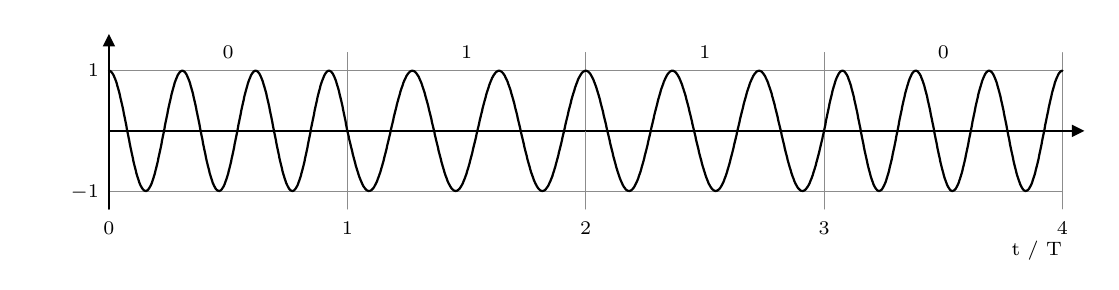
\begin{tikzpicture}[x=0.01985cm,y=-0.01985cm,line cap=round,line join=round]
\useasboundingbox (0,0) rectangle (680,150);
\path[draw=black!45,line width=0.35pt] (52,116) -- (52,16);
\path[draw=black!45,line width=0.35pt] (204.5,116) -- (204.5,16);
\path[draw=black!45,line width=0.35pt] (357,116) -- (357,16);
\path[draw=black!45,line width=0.35pt] (509.5,116) -- (509.5,16);
\path[draw=black!45,line width=0.35pt] (662,116) -- (662,16);
\path[draw=black!45,line width=0.35pt] (52,27.5) -- (662,27.5);
\path[draw=black!45,line width=0.35pt] (52,104.5) -- (662,104.5);
\path[draw=black,line width=0.7pt] (52,66) -- (670,66);
\path[fill=black,draw=none] (676,66) -- (668,62) -- (668,70) -- cycle;
\path[draw=black,line width=0.7pt] (52,116) -- (52,10);
\path[fill=black,draw=none] (52,4) -- (48,12) -- (56,12) -- cycle;
\node[anchor=base,inner sep=0pt,font=\scriptsize] at (52,132) {0};
\node[anchor=base,inner sep=0pt,font=\scriptsize] at (204.5,132) {1};
\node[anchor=base,inner sep=0pt,font=\scriptsize] at (357,132) {2};
\node[anchor=base,inner sep=0pt,font=\scriptsize] at (509.5,132) {3};
\node[anchor=base,inner sep=0pt,font=\scriptsize] at (662,132) {4};
\node[anchor=base east,inner sep=0pt,font=\scriptsize] at (46,31.5) {1};
\node[anchor=base east,inner sep=0pt,font=\scriptsize] at (46,108.5) {$-$1};
\node[anchor=base east,inner sep=0pt,font=\scriptsize] at (662,146) {t / T};
\path[draw=black!45,line width=0.35pt,dash pattern=on 3pt off 2pt] (204.5,116) -- (204.5,16);
\path[draw=black!45,line width=0.35pt,dash pattern=on 3pt off 2pt] (357,116) -- (357,16);
\path[draw=black!45,line width=0.35pt,dash pattern=on 3pt off 2pt] (509.5,116) -- (509.5,16);
\path[draw=black,line width=0.8pt] (52,27.5) -- (52.4,27.6) -- (52.8,27.7) -- (53.1,28) -- (53.5,28.3) -- (53.9,28.8) -- (54.3,29.3) -- (54.7,30) -- (55.1,30.7) -- (55.4,31.5) -- (55.8,32.4) -- (56.2,33.4) -- (56.6,34.5) -- (57,35.7) -- (57.3,37) -- (57.7,38.3) -- (58.1,39.7) -- (58.5,41.1) -- (58.9,42.7) -- (59.2,44.3) -- (59.6,45.9) -- (60,47.6) -- (60.4,49.4) -- (60.8,51.1) -- (61.2,53) -- (61.5,54.8) -- (61.9,56.7) -- (62.3,58.6) -- (62.7,60.6) -- (63.1,62.5) -- (63.4,64.5) -- (63.8,66.5) -- (64.2,68.4) -- (64.6,70.4) -- (65,72.3) -- (65.3,74.2) -- (65.7,76.1) -- (66.1,78) -- (66.5,79.9) -- (66.9,81.7) -- (67.3,83.5) -- (67.6,85.2) -- (68,86.9) -- (68.4,88.5) -- (68.8,90) -- (69.2,91.5) -- (69.5,93) -- (69.9,94.3) -- (70.3,95.6) -- (70.7,96.8) -- (71.1,98) -- (71.4,99) -- (71.8,100) -- (72.2,100.9) -- (72.6,101.6) -- (73,102.3) -- (73.4,102.9) -- (73.7,103.4) -- (74.1,103.8) -- (74.5,104.1) -- (74.9,104.3) -- (75.3,104.4) -- (75.6,104.5) -- (76,104.4) -- (76.4,104.2) -- (76.8,103.9) -- (77.2,103.5) -- (77.5,103) -- (77.9,102.4) -- (78.3,101.7) -- (78.7,100.9) -- (79.1,100.1) -- (79.5,99.1) -- (79.8,98.1) -- (80.2,96.9) -- (80.6,95.7) -- (81,94.4) -- (81.4,93.1) -- (81.7,91.7) -- (82.1,90.2) -- (82.5,88.6) -- (82.9,87) -- (83.3,85.3) -- (83.6,83.6) -- (84,81.8) -- (84.4,80) -- (84.8,78.2) -- (85.2,76.3) -- (85.6,74.4) -- (85.9,72.5) -- (86.3,70.5) -- (86.7,68.6) -- (87.1,66.6) -- (87.5,64.6) -- (87.8,62.7) -- (88.2,60.7) -- (88.6,58.8) -- (89,56.9) -- (89.4,55) -- (89.7,53.1) -- (90.1,51.3) -- (90.5,49.5) -- (90.9,47.7) -- (91.3,46) -- (91.7,44.4) -- (92,42.8) -- (92.4,41.3) -- (92.8,39.8) -- (93.2,38.4) -- (93.6,37) -- (93.9,35.8) -- (94.3,34.6) -- (94.7,33.5) -- (95.1,32.5) -- (95.5,31.6) -- (95.8,30.8) -- (96.2,30) -- (96.6,29.4) -- (97,28.8) -- (97.4,28.4) -- (97.8,28) -- (98.1,27.8) -- (98.5,27.6) -- (98.9,27.5) -- (99.3,27.6) -- (99.7,27.7) -- (100,28) -- (100.4,28.3) -- (100.8,28.7) -- (101.2,29.3) -- (101.6,29.9) -- (101.9,30.6) -- (102.3,31.5) -- (102.7,32.4) -- (103.1,33.4) -- (103.5,34.4) -- (103.9,35.6) -- (104.2,36.9) -- (104.6,38.2) -- (105,39.6) -- (105.4,41) -- (105.8,42.5) -- (106.1,44.1) -- (106.5,45.8) -- (106.9,47.5) -- (107.3,49.2) -- (107.7,51) -- (108,52.8) -- (108.4,54.7) -- (108.8,56.6) -- (109.2,58.5) -- (109.6,60.4) -- (110,62.4) -- (110.3,64.3) -- (110.7,66.3) -- (111.1,68.3) -- (111.5,70.2) -- (111.9,72.2) -- (112.2,74.1) -- (112.6,76) -- (113,77.9) -- (113.4,79.7) -- (113.8,81.6) -- (114.1,83.3) -- (114.5,85.1) -- (114.9,86.7) -- (115.3,88.4) -- (115.7,89.9) -- (116.1,91.4) -- (116.4,92.9) -- (116.8,94.2) -- (117.2,95.5) -- (117.6,96.8) -- (118,97.9) -- (118.3,99) -- (118.7,99.9) -- (119.1,100.8) -- (119.5,101.6) -- (119.9,102.3) -- (120.2,102.9) -- (120.6,103.4) -- (121,103.8) -- (121.4,104.1) -- (121.8,104.3) -- (122.2,104.4) -- (122.5,104.5) -- (122.9,104.4) -- (123.3,104.2) -- (123.7,103.9) -- (124.1,103.5) -- (124.4,103) -- (124.8,102.4) -- (125.2,101.8) -- (125.6,101) -- (126,100.1) -- (126.3,99.2) -- (126.7,98.1) -- (127.1,97) -- (127.5,95.8) -- (127.9,94.5) -- (128.3,93.2) -- (128.6,91.8) -- (129,90.3) -- (129.4,88.7) -- (129.8,87.1) -- (130.2,85.4) -- (130.5,83.7) -- (130.9,82) -- (131.3,80.2) -- (131.7,78.3) -- (132.1,76.4) -- (132.4,74.5) -- (132.8,72.6) -- (133.2,70.7) -- (133.6,68.7) -- (134,66.8) -- (134.4,64.8) -- (134.7,62.8) -- (135.1,60.9) -- (135.5,58.9) -- (135.9,57) -- (136.3,55.1) -- (136.6,53.3) -- (137,51.4) -- (137.4,49.6) -- (137.8,47.9) -- (138.2,46.2) -- (138.5,44.5) -- (138.9,42.9) -- (139.3,41.4) -- (139.7,39.9) -- (140.1,38.5) -- (140.5,37.1) -- (140.8,35.9) -- (141.2,34.7) -- (141.6,33.6) -- (142,32.6) -- (142.4,31.7) -- (142.7,30.8) -- (143.1,30.1) -- (143.5,29.4) -- (143.9,28.9) -- (144.3,28.4) -- (144.6,28) -- (145,27.8) -- (145.4,27.6) -- (145.8,27.5) -- (146.2,27.6) -- (146.6,27.7) -- (146.9,27.9) -- (147.3,28.3) -- (147.7,28.7) -- (148.1,29.2) -- (148.5,29.9) -- (148.8,30.6) -- (149.2,31.4) -- (149.6,32.3) -- (150,33.3) -- (150.4,34.4) -- (150.7,35.5) -- (151.1,36.8) -- (151.5,38.1) -- (151.9,39.5) -- (152.3,40.9) -- (152.7,42.4) -- (153,44) -- (153.4,45.6) -- (153.8,47.3) -- (154.2,49.1) -- (154.6,50.9) -- (154.9,52.7) -- (155.3,54.5) -- (155.7,56.4) -- (156.1,58.3) -- (156.5,60.3) -- (156.8,62.2) -- (157.2,64.2) -- (157.6,66.2) -- (158,68.1) -- (158.4,70.1) -- (158.8,72) -- (159.1,73.9) -- (159.5,75.9) -- (159.9,77.7) -- (160.3,79.6) -- (160.7,81.4) -- (161,83.2) -- (161.4,84.9) -- (161.8,86.6) -- (162.2,88.2) -- (162.6,89.8) -- (162.9,91.3) -- (163.3,92.8) -- (163.7,94.1) -- (164.1,95.4) -- (164.5,96.7) -- (164.9,97.8) -- (165.2,98.9) -- (165.6,99.8) -- (166,100.7) -- (166.4,101.5) -- (166.8,102.2) -- (167.1,102.8) -- (167.5,103.4) -- (167.9,103.8) -- (168.3,104.1) -- (168.7,104.3) -- (169,104.4) -- (169.4,104.5) -- (169.8,104.4) -- (170.2,104.2) -- (170.6,103.9) -- (171,103.5) -- (171.3,103.1) -- (171.7,102.5) -- (172.1,101.8) -- (172.5,101.1) -- (172.9,100.2) -- (173.2,99.3) -- (173.6,98.2) -- (174,97.1) -- (174.4,95.9) -- (174.8,94.6) -- (175.1,93.3) -- (175.5,91.9) -- (175.9,90.4) -- (176.3,88.9) -- (176.7,87.2) -- (177.1,85.6) -- (177.4,83.9) -- (177.8,82.1) -- (178.2,80.3) -- (178.6,78.5) -- (179,76.6) -- (179.3,74.7) -- (179.7,72.8) -- (180.1,70.8) -- (180.5,68.9) -- (180.9,66.9) -- (181.2,64.9) -- (181.6,63) -- (182,61) -- (182.4,59.1) -- (182.8,57.2) -- (183.2,55.3) -- (183.5,53.4) -- (183.9,51.6) -- (184.3,49.8) -- (184.7,48) -- (185.1,46.3) -- (185.4,44.6) -- (185.8,43) -- (186.2,41.5) -- (186.6,40) -- (187,38.6) -- (187.3,37.2) -- (187.7,36) -- (188.1,34.8) -- (188.5,33.7) -- (188.9,32.7) -- (189.3,31.7) -- (189.6,30.9) -- (190,30.1) -- (190.4,29.5) -- (190.8,28.9) -- (191.2,28.4) -- (191.5,28.1) -- (191.9,27.8) -- (192.3,27.6) -- (192.7,27.5) -- (193.1,27.6) -- (193.4,27.7) -- (193.8,27.9) -- (194.2,28.2) -- (194.6,28.7) -- (195,29.2) -- (195.4,29.8) -- (195.7,30.5) -- (196.1,31.3) -- (196.5,32.2) -- (196.9,33.2) -- (197.3,34.3) -- (197.6,35.4) -- (198,36.7) -- (198.4,38) -- (198.8,39.3) -- (199.2,40.8) -- (199.5,42.3) -- (199.9,43.9) -- (200.3,45.5) -- (200.7,47.2) -- (201.1,48.9) -- (201.5,50.7) -- (201.8,52.5) -- (202.2,54.4) -- (202.6,56.3) -- (203,58.2) -- (203.4,60.1) -- (203.7,62.1) -- (204.1,64) -- (204.5,66) -- (204.9,67.7) -- (205.3,69.3) -- (205.6,71) -- (206,72.6) -- (206.4,74.2) -- (206.8,75.9) -- (207.2,77.5) -- (207.6,79) -- (207.9,80.6) -- (208.3,82.1) -- (208.7,83.6) -- (209.1,85.1) -- (209.5,86.5) -- (209.8,87.9) -- (210.2,89.2) -- (210.6,90.5) -- (211,91.8) -- (211.4,93) -- (211.7,94.1) -- (212.1,95.2) -- (212.5,96.3) -- (212.9,97.3) -- (213.3,98.2) -- (213.7,99.1) -- (214,99.9) -- (214.4,100.7) -- (214.8,101.4) -- (215.2,102) -- (215.6,102.5) -- (215.9,103) -- (216.3,103.4) -- (216.7,103.8) -- (217.1,104.1) -- (217.5,104.3) -- (217.8,104.4) -- (218.2,104.5) -- (218.6,104.4) -- (219,104.4) -- (219.4,104.2) -- (219.8,104) -- (220.1,103.7) -- (220.5,103.3) -- (220.9,102.9) -- (221.3,102.4) -- (221.7,101.8) -- (222,101.2) -- (222.4,100.5) -- (222.8,99.7) -- (223.2,98.9) -- (223.6,98) -- (223.9,97) -- (224.3,96) -- (224.7,95) -- (225.1,93.8) -- (225.5,92.7) -- (225.9,91.4) -- (226.2,90.2) -- (226.6,88.9) -- (227,87.5) -- (227.4,86.1) -- (227.8,84.7) -- (228.1,83.2) -- (228.5,81.7) -- (228.9,80.2) -- (229.3,78.6) -- (229.7,77) -- (230,75.4) -- (230.4,73.8) -- (230.8,72.2) -- (231.2,70.5) -- (231.6,68.9) -- (232,67.2) -- (232.3,65.5) -- (232.7,63.9) -- (233.1,62.2) -- (233.5,60.6) -- (233.9,58.9) -- (234.2,57.3) -- (234.6,55.7) -- (235,54.1) -- (235.4,52.5) -- (235.8,51) -- (236.1,49.5) -- (236.5,48) -- (236.9,46.6) -- (237.3,45.1) -- (237.7,43.8) -- (238.1,42.4) -- (238.4,41.1) -- (238.8,39.9) -- (239.2,38.7) -- (239.6,37.6) -- (240,36.5) -- (240.3,35.4) -- (240.7,34.4) -- (241.1,33.5) -- (241.5,32.7) -- (241.9,31.9) -- (242.2,31.1) -- (242.6,30.5) -- (243,29.9) -- (243.4,29.3) -- (243.8,28.9) -- (244.2,28.5) -- (244.5,28.1) -- (244.9,27.9) -- (245.3,27.7) -- (245.7,27.6) -- (246.1,27.5) -- (246.4,27.6) -- (246.8,27.7) -- (247.2,27.8) -- (247.6,28.1) -- (248,28.4) -- (248.3,28.8) -- (248.7,29.2) -- (249.1,29.8) -- (249.5,30.4) -- (249.9,31) -- (250.3,31.7) -- (250.6,32.5) -- (251,33.4) -- (251.4,34.3) -- (251.8,35.2) -- (252.2,36.3) -- (252.5,37.4) -- (252.9,38.5) -- (253.3,39.7) -- (253.7,40.9) -- (254.1,42.2) -- (254.4,43.5) -- (254.8,44.9) -- (255.2,46.3) -- (255.6,47.7) -- (256,49.2) -- (256.4,50.7) -- (256.7,52.3) -- (257.1,53.8) -- (257.5,55.4) -- (257.9,57) -- (258.3,58.6) -- (258.6,60.3) -- (259,61.9) -- (259.4,63.6) -- (259.8,65.2) -- (260.2,66.9) -- (260.5,68.6) -- (260.9,70.2) -- (261.3,71.9) -- (261.7,73.5) -- (262.1,75.1) -- (262.5,76.7) -- (262.8,78.3) -- (263.2,79.9) -- (263.6,81.4) -- (264,82.9) -- (264.4,84.4) -- (264.7,85.8) -- (265.1,87.2) -- (265.5,88.6) -- (265.9,89.9) -- (266.3,91.2) -- (266.6,92.4) -- (267,93.6) -- (267.4,94.8) -- (267.8,95.8) -- (268.2,96.8) -- (268.5,97.8) -- (268.9,98.7) -- (269.3,99.6) -- (269.7,100.3) -- (270.1,101.1) -- (270.5,101.7) -- (270.8,102.3) -- (271.2,102.8) -- (271.6,103.3) -- (272,103.6) -- (272.4,103.9) -- (272.7,104.2) -- (273.1,104.3) -- (273.5,104.4) -- (273.9,104.5) -- (274.3,104.4) -- (274.7,104.3) -- (275,104.1) -- (275.4,103.8) -- (275.8,103.5) -- (276.2,103.1) -- (276.6,102.6) -- (276.9,102.1) -- (277.3,101.5) -- (277.7,100.8) -- (278.1,100.1) -- (278.5,99.3) -- (278.8,98.4) -- (279.2,97.5) -- (279.6,96.5) -- (280,95.4) -- (280.4,94.3) -- (280.8,93.2) -- (281.1,92) -- (281.5,90.7) -- (281.9,89.5) -- (282.3,88.1) -- (282.7,86.7) -- (283,85.3) -- (283.4,83.9) -- (283.8,82.4) -- (284.2,80.9) -- (284.6,79.3) -- (284.9,77.7) -- (285.3,76.1) -- (285.7,74.5) -- (286.1,72.9) -- (286.5,71.3) -- (286.9,69.6) -- (287.2,68) -- (287.6,66.3) -- (288,64.6) -- (288.4,63) -- (288.8,61.3) -- (289.1,59.7) -- (289.5,58.1) -- (289.9,56.4) -- (290.3,54.8) -- (290.7,53.3) -- (291,51.7) -- (291.4,50.2) -- (291.8,48.7) -- (292.2,47.2) -- (292.6,45.8) -- (293,44.4) -- (293.3,43) -- (293.7,41.7) -- (294.1,40.5) -- (294.5,39.2) -- (294.9,38.1) -- (295.2,37) -- (295.6,35.9) -- (296,34.9) -- (296.4,33.9) -- (296.8,33) -- (297.1,32.2) -- (297.5,31.5) -- (297.9,30.8) -- (298.3,30.1) -- (298.7,29.6) -- (299.1,29.1) -- (299.4,28.6) -- (299.8,28.3) -- (300.2,28) -- (300.6,27.8) -- (301,27.6) -- (301.3,27.5) -- (301.7,27.5) -- (302.1,27.6) -- (302.5,27.8) -- (302.9,28) -- (303.2,28.2) -- (303.6,28.6) -- (304,29) -- (304.4,29.5) -- (304.8,30.1) -- (305.2,30.7) -- (305.5,31.4) -- (305.9,32.2) -- (306.3,33) -- (306.7,33.9) -- (307.1,34.8) -- (307.4,35.8) -- (307.8,36.9) -- (308.2,38) -- (308.6,39.1) -- (309,40.3) -- (309.3,41.6) -- (309.7,42.9) -- (310.1,44.3) -- (310.5,45.6) -- (310.9,47.1) -- (311.3,48.5) -- (311.6,50) -- (312,51.6) -- (312.4,53.1) -- (312.8,54.7) -- (313.2,56.3) -- (313.5,57.9) -- (313.9,59.5) -- (314.3,61.2) -- (314.7,62.8) -- (315.1,64.5) -- (315.4,66.2) -- (315.8,67.8) -- (316.2,69.5) -- (316.6,71.1) -- (317,72.8) -- (317.4,74.4) -- (317.7,76) -- (318.1,77.6) -- (318.5,79.2) -- (318.9,80.7) -- (319.3,82.2) -- (319.6,83.7) -- (320,85.2) -- (320.4,86.6) -- (320.8,88) -- (321.2,89.3) -- (321.5,90.6) -- (321.9,91.9) -- (322.3,93.1) -- (322.7,94.2) -- (323.1,95.3) -- (323.5,96.4) -- (323.8,97.4) -- (324.2,98.3) -- (324.6,99.2) -- (325,100) -- (325.4,100.7) -- (325.7,101.4) -- (326.1,102) -- (326.5,102.6) -- (326.9,103.1) -- (327.3,103.5) -- (327.6,103.8) -- (328,104.1) -- (328.4,104.3) -- (328.8,104.4) -- (329.2,104.5) -- (329.6,104.4) -- (329.9,104.4) -- (330.3,104.2) -- (330.7,104) -- (331.1,103.7) -- (331.5,103.3) -- (331.8,102.8) -- (332.2,102.3) -- (332.6,101.8) -- (333,101.1) -- (333.4,100.4) -- (333.7,99.6) -- (334.1,98.8) -- (334.5,97.9) -- (334.9,96.9) -- (335.3,95.9) -- (335.7,94.9) -- (336,93.7) -- (336.4,92.5) -- (336.8,91.3) -- (337.2,90) -- (337.6,88.7) -- (337.9,87.4) -- (338.3,86) -- (338.7,84.5) -- (339.1,83.1) -- (339.5,81.6) -- (339.8,80) -- (340.2,78.5) -- (340.6,76.9) -- (341,75.3) -- (341.4,73.7) -- (341.8,72) -- (342.1,70.4) -- (342.5,68.7) -- (342.9,67.1) -- (343.3,65.4) -- (343.7,63.7) -- (344,62.1) -- (344.4,60.4) -- (344.8,58.8) -- (345.2,57.2) -- (345.6,55.6) -- (345.9,54) -- (346.3,52.4) -- (346.7,50.9) -- (347.1,49.4) -- (347.5,47.9) -- (347.8,46.4) -- (348.2,45) -- (348.6,43.6) -- (349,42.3) -- (349.4,41) -- (349.8,39.8) -- (350.1,38.6) -- (350.5,37.5) -- (350.9,36.4) -- (351.3,35.3) -- (351.7,34.4) -- (352,33.4) -- (352.4,32.6) -- (352.8,31.8) -- (353.2,31.1) -- (353.6,30.4) -- (354,29.8) -- (354.3,29.3) -- (354.7,28.8) -- (355.1,28.4) -- (355.5,28.1) -- (355.9,27.9) -- (356.2,27.7) -- (356.6,27.6) -- (357,27.5) -- (357.4,27.6) -- (357.8,27.7) -- (358.1,27.9) -- (358.5,28.1) -- (358.9,28.4) -- (359.3,28.8) -- (359.7,29.3) -- (360.1,29.8) -- (360.4,30.4) -- (360.8,31.1) -- (361.2,31.8) -- (361.6,32.6) -- (362,33.4) -- (362.3,34.4) -- (362.7,35.3) -- (363.1,36.4) -- (363.5,37.5) -- (363.9,38.6) -- (364.2,39.8) -- (364.6,41) -- (365,42.3) -- (365.4,43.6) -- (365.8,45) -- (366.2,46.4) -- (366.5,47.9) -- (366.9,49.4) -- (367.3,50.9) -- (367.7,52.4) -- (368.1,54) -- (368.4,55.6) -- (368.8,57.2) -- (369.2,58.8) -- (369.6,60.4) -- (370,62.1) -- (370.3,63.7) -- (370.7,65.4) -- (371.1,67.1) -- (371.5,68.7) -- (371.9,70.4) -- (372.3,72) -- (372.6,73.7) -- (373,75.3) -- (373.4,76.9) -- (373.8,78.5) -- (374.2,80) -- (374.5,81.6) -- (374.9,83.1) -- (375.3,84.5) -- (375.7,86) -- (376.1,87.4) -- (376.4,88.7) -- (376.8,90) -- (377.2,91.3) -- (377.6,92.5) -- (378,93.7) -- (378.4,94.9) -- (378.7,95.9) -- (379.1,96.9) -- (379.5,97.9) -- (379.9,98.8) -- (380.3,99.6) -- (380.6,100.4) -- (381,101.1) -- (381.4,101.8) -- (381.8,102.3) -- (382.2,102.8) -- (382.5,103.3) -- (382.9,103.7) -- (383.3,104) -- (383.7,104.2) -- (384.1,104.4) -- (384.5,104.4) -- (384.8,104.5) -- (385.2,104.4) -- (385.6,104.3) -- (386,104.1) -- (386.4,103.8) -- (386.7,103.5) -- (387.1,103.1) -- (387.5,102.6) -- (387.9,102) -- (388.3,101.4) -- (388.6,100.7) -- (389,100) -- (389.4,99.2) -- (389.8,98.3) -- (390.2,97.4) -- (390.6,96.4) -- (390.9,95.3) -- (391.3,94.2) -- (391.7,93.1) -- (392.1,91.9) -- (392.5,90.6) -- (392.8,89.3) -- (393.2,88) -- (393.6,86.6) -- (394,85.2) -- (394.4,83.7) -- (394.7,82.2) -- (395.1,80.7) -- (395.5,79.2) -- (395.9,77.6) -- (396.3,76) -- (396.7,74.4) -- (397,72.8) -- (397.4,71.1) -- (397.8,69.5) -- (398.2,67.8) -- (398.6,66.2) -- (398.9,64.5) -- (399.3,62.8) -- (399.7,61.2) -- (400.1,59.5) -- (400.5,57.9) -- (400.8,56.3) -- (401.2,54.7) -- (401.6,53.1) -- (402,51.6) -- (402.4,50) -- (402.8,48.5) -- (403.1,47.1) -- (403.5,45.6) -- (403.9,44.3) -- (404.3,42.9) -- (404.7,41.6) -- (405,40.3) -- (405.4,39.1) -- (405.8,38) -- (406.2,36.9) -- (406.6,35.8) -- (406.9,34.8) -- (407.3,33.9) -- (407.7,33) -- (408.1,32.2) -- (408.5,31.4) -- (408.8,30.7) -- (409.2,30.1) -- (409.6,29.5) -- (410,29) -- (410.4,28.6) -- (410.8,28.2) -- (411.1,28) -- (411.5,27.8) -- (411.9,27.6) -- (412.3,27.5) -- (412.7,27.5) -- (413,27.6) -- (413.4,27.8) -- (413.8,28) -- (414.2,28.3) -- (414.6,28.6) -- (415,29.1) -- (415.3,29.6) -- (415.7,30.1) -- (416.1,30.8) -- (416.5,31.5) -- (416.9,32.2) -- (417.2,33) -- (417.6,33.9) -- (418,34.9) -- (418.4,35.9) -- (418.8,37) -- (419.1,38.1) -- (419.5,39.2) -- (419.9,40.5) -- (420.3,41.7) -- (420.7,43) -- (421.1,44.4) -- (421.4,45.8) -- (421.8,47.2) -- (422.2,48.7) -- (422.6,50.2) -- (423,51.7) -- (423.3,53.3) -- (423.7,54.8) -- (424.1,56.4) -- (424.5,58.1) -- (424.9,59.7) -- (425.2,61.3) -- (425.6,63) -- (426,64.6) -- (426.4,66.3) -- (426.8,68) -- (427.2,69.6) -- (427.5,71.3) -- (427.9,72.9) -- (428.3,74.5) -- (428.7,76.1) -- (429.1,77.7) -- (429.4,79.3) -- (429.8,80.9) -- (430.2,82.4) -- (430.6,83.9) -- (431,85.3) -- (431.3,86.7) -- (431.7,88.1) -- (432.1,89.5) -- (432.5,90.7) -- (432.9,92) -- (433.3,93.2) -- (433.6,94.3) -- (434,95.4) -- (434.4,96.5) -- (434.8,97.5) -- (435.2,98.4) -- (435.5,99.3) -- (435.9,100.1) -- (436.3,100.8) -- (436.7,101.5) -- (437.1,102.1) -- (437.4,102.6) -- (437.8,103.1) -- (438.2,103.5) -- (438.6,103.8) -- (439,104.1) -- (439.4,104.3) -- (439.7,104.4) -- (440.1,104.5) -- (440.5,104.4) -- (440.9,104.3) -- (441.3,104.2) -- (441.6,103.9) -- (442,103.6) -- (442.4,103.3) -- (442.8,102.8) -- (443.2,102.3) -- (443.5,101.7) -- (443.9,101.1) -- (444.3,100.3) -- (444.7,99.6) -- (445.1,98.7) -- (445.5,97.8) -- (445.8,96.8) -- (446.2,95.8) -- (446.6,94.8) -- (447,93.6) -- (447.4,92.4) -- (447.7,91.2) -- (448.1,89.9) -- (448.5,88.6) -- (448.9,87.2) -- (449.3,85.8) -- (449.6,84.4) -- (450,82.9) -- (450.4,81.4) -- (450.8,79.9) -- (451.2,78.3) -- (451.6,76.7) -- (451.9,75.1) -- (452.3,73.5) -- (452.7,71.9) -- (453.1,70.2) -- (453.5,68.6) -- (453.8,66.9) -- (454.2,65.2) -- (454.6,63.6) -- (455,61.9) -- (455.4,60.3) -- (455.7,58.6) -- (456.1,57) -- (456.5,55.4) -- (456.9,53.8) -- (457.3,52.3) -- (457.7,50.7) -- (458,49.2) -- (458.4,47.7) -- (458.8,46.3) -- (459.2,44.9) -- (459.6,43.5) -- (459.9,42.2) -- (460.3,40.9) -- (460.7,39.7) -- (461.1,38.5) -- (461.5,37.4) -- (461.8,36.3) -- (462.2,35.2) -- (462.6,34.3) -- (463,33.4) -- (463.4,32.5) -- (463.8,31.7) -- (464.1,31) -- (464.5,30.4) -- (464.9,29.8) -- (465.3,29.2) -- (465.7,28.8) -- (466,28.4) -- (466.4,28.1) -- (466.8,27.8) -- (467.2,27.7) -- (467.6,27.6) -- (467.9,27.5) -- (468.3,27.6) -- (468.7,27.7) -- (469.1,27.9) -- (469.5,28.1) -- (469.9,28.5) -- (470.2,28.9) -- (470.6,29.3) -- (471,29.9) -- (471.4,30.5) -- (471.8,31.1) -- (472.1,31.9) -- (472.5,32.7) -- (472.9,33.5) -- (473.3,34.4) -- (473.7,35.4) -- (474,36.5) -- (474.4,37.6) -- (474.8,38.7) -- (475.2,39.9) -- (475.6,41.1) -- (476,42.4) -- (476.3,43.8) -- (476.7,45.1) -- (477.1,46.6) -- (477.5,48) -- (477.9,49.5) -- (478.2,51) -- (478.6,52.5) -- (479,54.1) -- (479.4,55.7) -- (479.8,57.3) -- (480.1,58.9) -- (480.5,60.6) -- (480.9,62.2) -- (481.3,63.9) -- (481.7,65.5) -- (482.1,67.2) -- (482.4,68.9) -- (482.8,70.5) -- (483.2,72.2) -- (483.6,73.8) -- (484,75.4) -- (484.3,77) -- (484.7,78.6) -- (485.1,80.2) -- (485.5,81.7) -- (485.9,83.2) -- (486.2,84.7) -- (486.6,86.1) -- (487,87.5) -- (487.4,88.9) -- (487.8,90.2) -- (488.2,91.4) -- (488.5,92.7) -- (488.9,93.8) -- (489.3,95) -- (489.7,96) -- (490.1,97) -- (490.4,98) -- (490.8,98.9) -- (491.2,99.7) -- (491.6,100.5) -- (492,101.2) -- (492.3,101.8) -- (492.7,102.4) -- (493.1,102.9) -- (493.5,103.3) -- (493.9,103.7) -- (494.3,104) -- (494.6,104.2) -- (495,104.4) -- (495.4,104.4) -- (495.8,104.5) -- (496.2,104.4) -- (496.5,104.3) -- (496.9,104.1) -- (497.3,103.8) -- (497.7,103.4) -- (498.1,103) -- (498.4,102.5) -- (498.8,102) -- (499.2,101.4) -- (499.6,100.7) -- (500,99.9) -- (500.4,99.1) -- (500.7,98.2) -- (501.1,97.3) -- (501.5,96.3) -- (501.9,95.2) -- (502.3,94.1) -- (502.6,93) -- (503,91.8) -- (503.4,90.5) -- (503.8,89.2) -- (504.2,87.9) -- (504.5,86.5) -- (504.9,85.1) -- (505.3,83.6) -- (505.7,82.1) -- (506.1,80.6) -- (506.5,79) -- (506.8,77.5) -- (507.2,75.9) -- (507.6,74.2) -- (508,72.6) -- (508.4,71) -- (508.7,69.3) -- (509.1,67.7) -- (509.5,66) -- (509.9,64) -- (510.3,62.1) -- (510.6,60.1) -- (511,58.2) -- (511.4,56.3) -- (511.8,54.4) -- (512.2,52.5) -- (512.6,50.7) -- (512.9,48.9) -- (513.3,47.2) -- (513.7,45.5) -- (514.1,43.9) -- (514.5,42.3) -- (514.8,40.8) -- (515.2,39.3) -- (515.6,38) -- (516,36.7) -- (516.4,35.4) -- (516.7,34.3) -- (517.1,33.2) -- (517.5,32.2) -- (517.9,31.3) -- (518.3,30.5) -- (518.7,29.8) -- (519,29.2) -- (519.4,28.7) -- (519.8,28.2) -- (520.2,27.9) -- (520.6,27.7) -- (520.9,27.6) -- (521.3,27.5) -- (521.7,27.6) -- (522.1,27.8) -- (522.5,28.1) -- (522.8,28.4) -- (523.2,28.9) -- (523.6,29.5) -- (524,30.1) -- (524.4,30.9) -- (524.8,31.7) -- (525.1,32.7) -- (525.5,33.7) -- (525.9,34.8) -- (526.3,36) -- (526.7,37.2) -- (527,38.6) -- (527.4,40) -- (527.8,41.5) -- (528.2,43) -- (528.6,44.6) -- (528.9,46.3) -- (529.3,48) -- (529.7,49.8) -- (530.1,51.6) -- (530.5,53.4) -- (530.9,55.3) -- (531.2,57.2) -- (531.6,59.1) -- (532,61) -- (532.4,63) -- (532.8,64.9) -- (533.1,66.9) -- (533.5,68.9) -- (533.9,70.8) -- (534.3,72.8) -- (534.7,74.7) -- (535,76.6) -- (535.4,78.5) -- (535.8,80.3) -- (536.2,82.1) -- (536.6,83.9) -- (537,85.6) -- (537.3,87.2) -- (537.7,88.9) -- (538.1,90.4) -- (538.5,91.9) -- (538.9,93.3) -- (539.2,94.6) -- (539.6,95.9) -- (540,97.1) -- (540.4,98.2) -- (540.8,99.3) -- (541.1,100.2) -- (541.5,101.1) -- (541.9,101.8) -- (542.3,102.5) -- (542.7,103.1) -- (543.1,103.5) -- (543.4,103.9) -- (543.8,104.2) -- (544.2,104.4) -- (544.6,104.5) -- (545,104.4) -- (545.3,104.3) -- (545.7,104.1) -- (546.1,103.8) -- (546.5,103.4) -- (546.9,102.8) -- (547.2,102.2) -- (547.6,101.5) -- (548,100.7) -- (548.4,99.8) -- (548.8,98.9) -- (549.2,97.8) -- (549.5,96.7) -- (549.9,95.4) -- (550.3,94.1) -- (550.7,92.8) -- (551.1,91.3) -- (551.4,89.8) -- (551.8,88.2) -- (552.2,86.6) -- (552.6,84.9) -- (553,83.2) -- (553.3,81.4) -- (553.7,79.6) -- (554.1,77.7) -- (554.5,75.9) -- (554.9,73.9) -- (555.3,72) -- (555.6,70.1) -- (556,68.1) -- (556.4,66.2) -- (556.8,64.2) -- (557.2,62.2) -- (557.5,60.3) -- (557.9,58.3) -- (558.3,56.4) -- (558.7,54.5) -- (559.1,52.7) -- (559.4,50.9) -- (559.8,49.1) -- (560.2,47.3) -- (560.6,45.6) -- (561,44) -- (561.3,42.4) -- (561.7,40.9) -- (562.1,39.5) -- (562.5,38.1) -- (562.9,36.8) -- (563.3,35.5) -- (563.6,34.4) -- (564,33.3) -- (564.4,32.3) -- (564.8,31.4) -- (565.2,30.6) -- (565.5,29.9) -- (565.9,29.2) -- (566.3,28.7) -- (566.7,28.3) -- (567.1,27.9) -- (567.4,27.7) -- (567.8,27.6) -- (568.2,27.5) -- (568.6,27.6) -- (569,27.8) -- (569.4,28) -- (569.7,28.4) -- (570.1,28.9) -- (570.5,29.4) -- (570.9,30.1) -- (571.3,30.8) -- (571.6,31.7) -- (572,32.6) -- (572.4,33.6) -- (572.8,34.7) -- (573.2,35.9) -- (573.6,37.1) -- (573.9,38.5) -- (574.3,39.9) -- (574.7,41.4) -- (575.1,42.9) -- (575.5,44.5) -- (575.8,46.2) -- (576.2,47.9) -- (576.6,49.6) -- (577,51.4) -- (577.4,53.3) -- (577.7,55.1) -- (578.1,57) -- (578.5,58.9) -- (578.9,60.9) -- (579.3,62.8) -- (579.7,64.8) -- (580,66.8) -- (580.4,68.7) -- (580.8,70.7) -- (581.2,72.6) -- (581.6,74.5) -- (581.9,76.4) -- (582.3,78.3) -- (582.7,80.2) -- (583.1,82) -- (583.5,83.7) -- (583.8,85.4) -- (584.2,87.1) -- (584.6,88.7) -- (585,90.3) -- (585.4,91.8) -- (585.8,93.2) -- (586.1,94.5) -- (586.5,95.8) -- (586.9,97) -- (587.3,98.1) -- (587.7,99.2) -- (588,100.1) -- (588.4,101) -- (588.8,101.8) -- (589.2,102.4) -- (589.6,103) -- (589.9,103.5) -- (590.3,103.9) -- (590.7,104.2) -- (591.1,104.4) -- (591.5,104.5) -- (591.9,104.4) -- (592.2,104.3) -- (592.6,104.1) -- (593,103.8) -- (593.4,103.4) -- (593.8,102.9) -- (594.1,102.3) -- (594.5,101.6) -- (594.9,100.8) -- (595.3,99.9) -- (595.7,99) -- (596,97.9) -- (596.4,96.8) -- (596.8,95.5) -- (597.2,94.2) -- (597.6,92.9) -- (598,91.4) -- (598.3,89.9) -- (598.7,88.4) -- (599.1,86.7) -- (599.5,85.1) -- (599.9,83.3) -- (600.2,81.6) -- (600.6,79.7) -- (601,77.9) -- (601.4,76) -- (601.8,74.1) -- (602.1,72.2) -- (602.5,70.2) -- (602.9,68.3) -- (603.3,66.3) -- (603.7,64.3) -- (604.1,62.4) -- (604.4,60.4) -- (604.8,58.5) -- (605.2,56.6) -- (605.6,54.7) -- (606,52.8) -- (606.3,51) -- (606.7,49.2) -- (607.1,47.5) -- (607.5,45.8) -- (607.9,44.1) -- (608.2,42.5) -- (608.6,41) -- (609,39.6) -- (609.4,38.2) -- (609.8,36.9) -- (610.2,35.6) -- (610.5,34.4) -- (610.9,33.4) -- (611.3,32.4) -- (611.7,31.5) -- (612.1,30.6) -- (612.4,29.9) -- (612.8,29.3) -- (613.2,28.7) -- (613.6,28.3) -- (614,28) -- (614.3,27.7) -- (614.7,27.6) -- (615.1,27.5) -- (615.5,27.6) -- (615.9,27.8) -- (616.3,28) -- (616.6,28.4) -- (617,28.8) -- (617.4,29.4) -- (617.8,30) -- (618.2,30.8) -- (618.5,31.6) -- (618.9,32.5) -- (619.3,33.5) -- (619.7,34.6) -- (620.1,35.8) -- (620.4,37) -- (620.8,38.4) -- (621.2,39.8) -- (621.6,41.3) -- (622,42.8) -- (622.4,44.4) -- (622.7,46) -- (623.1,47.7) -- (623.5,49.5) -- (623.9,51.3) -- (624.3,53.1) -- (624.6,55) -- (625,56.9) -- (625.4,58.8) -- (625.8,60.7) -- (626.2,62.7) -- (626.5,64.6) -- (626.9,66.6) -- (627.3,68.6) -- (627.7,70.5) -- (628.1,72.5) -- (628.4,74.4) -- (628.8,76.3) -- (629.2,78.2) -- (629.6,80) -- (630,81.8) -- (630.4,83.6) -- (630.7,85.3) -- (631.1,87) -- (631.5,88.6) -- (631.9,90.2) -- (632.3,91.7) -- (632.6,93.1) -- (633,94.4) -- (633.4,95.7) -- (633.8,96.9) -- (634.2,98.1) -- (634.6,99.1) -- (634.9,100.1) -- (635.3,100.9) -- (635.7,101.7) -- (636.1,102.4) -- (636.5,103) -- (636.8,103.5) -- (637.2,103.9) -- (637.6,104.2) -- (638,104.4) -- (638.4,104.5) -- (638.7,104.4) -- (639.1,104.3) -- (639.5,104.1) -- (639.9,103.8) -- (640.3,103.4) -- (640.7,102.9) -- (641,102.3) -- (641.4,101.6) -- (641.8,100.9) -- (642.2,100) -- (642.6,99) -- (642.9,98) -- (643.3,96.8) -- (643.7,95.6) -- (644.1,94.3) -- (644.5,93) -- (644.8,91.5) -- (645.2,90) -- (645.6,88.5) -- (646,86.9) -- (646.4,85.2) -- (646.8,83.5) -- (647.1,81.7) -- (647.5,79.9) -- (647.9,78) -- (648.3,76.1) -- (648.7,74.2) -- (649,72.3) -- (649.4,70.4) -- (649.8,68.4) -- (650.2,66.5) -- (650.6,64.5) -- (650.9,62.5) -- (651.3,60.6) -- (651.7,58.6) -- (652.1,56.7) -- (652.5,54.8) -- (652.9,53) -- (653.2,51.1) -- (653.6,49.4) -- (654,47.6) -- (654.4,45.9) -- (654.8,44.3) -- (655.1,42.7) -- (655.5,41.1) -- (655.9,39.7) -- (656.3,38.3) -- (656.7,37) -- (657,35.7) -- (657.4,34.5) -- (657.8,33.4) -- (658.2,32.4) -- (658.6,31.5) -- (659,30.7) -- (659.3,30) -- (659.7,29.3) -- (660.1,28.8) -- (660.5,28.3) -- (660.9,28) -- (661.2,27.7) -- (661.6,27.6) -- (662,27.5);
\node[anchor=base,inner sep=0pt,font=\scriptsize] at (128.3,20) {0};
\node[anchor=base,inner sep=0pt,font=\scriptsize] at (280.8,20) {1};
\node[anchor=base,inner sep=0pt,font=\scriptsize] at (433.3,20) {1};
\node[anchor=base,inner sep=0pt,font=\scriptsize] at (585.8,20) {0};
\end{tikzpicture}\end{center}
\begin{itemize}
\item Bitenként 3,25, illetve 2,75 periódus. A fázis folytonos marad, nincs ugrás a bithatáron.
\end{itemize}
\end{rajz}
\begin{figyelem}[Javítás]
A gyűjtemény $2(F+f_D)=400$ kHz-et ad: a Carson-képletbe a vivőt tette a moduláló frekvencia helyére.
\end{figyelem}
\begin{eredmeny}

\begin{center}\adjustbox{max width=\linewidth}{$\displaystyle \text{a) }200\ \text{és}\ 100\ \text{kHz}\qquad\text{b) }B_v\approx150\ \text{kHz}\qquad\text{c) }f_D=12{,}5\ \text{kHz: }162{,}5\ \text{és}\ 137{,}5\ \text{kHz}$}\end{center}
\end{eredmeny}


% ------------------------------------------------------------------
\section{\texorpdfstring{7.4. feladat: OOK, BPSK, FSK egymás alatt (hivatalos megoldás)}{7.4. feladat: OOK, BPSK, FSK egymás alatt (hivatalos megoldás)}}\label{ai7_04}
\setcounter{lepes}{0}
\begin{feladat}{7.4. feladat}
Rajzolja fel a $d_k=\{1,0,1,1,0\}$ sorozat OOK, BPSK és FSK jelét! Az első kettőnél a vivő a jelzési sebesség, FSK-nál $f_0=1/T$, $f_1=1{,}5/T$. Mekkora az FSK löket?

{\footnotesize\sffamily Forrás: ALL-IN 126. oldal $\cdot$ aiD\_7\_9. Címkék: vizsga}
\end{feladat}
\begin{keresunk}
\begin{itemize}
\item a három jel, és $f_D$ (frekvencialöket)
\end{itemize}
\end{keresunk}
\begin{jeloles}
\begin{jeltabla}
$\ca{f_v}$ & vivőfrekvencia & $1$\\
$T$ & jelzési (bit-) idő & \\
$\cb{f_0}$ & a 0-s bit frekvenciája & $1$\\
$\cc{f_1}$ & az 1-es bit frekvenciája & $1{,}5$\\
$f_D$ & frekvencialöket & \emph{keresett}\\
$d_k$ & a k-adik bit & \\
\end{jeltabla}
\end{jeloles}

\lepes{A jelek}
OOK: 1-nél van vivő, 0-nál nincs. BPSK: 1-nél $+\cos$, 0-nál $-\cos$. FSK: 0-nál 1 periódus, 1-nél 1,5 periódus bitenként, a fázis a bithatáron folytonos.

\lepes{Löket}


\begin{center}\adjustbox{max width=\linewidth}{$\displaystyle f_D=\frac12\left(\frac{1{,}5}{T}-\frac1T\right)=\frac1{4T}$}\end{center}
\jegyzet{definíció}{$f_DT=1/4$: ez éppen MSK}

\begin{rajz}
\textbf{OOK}\par
\begin{center}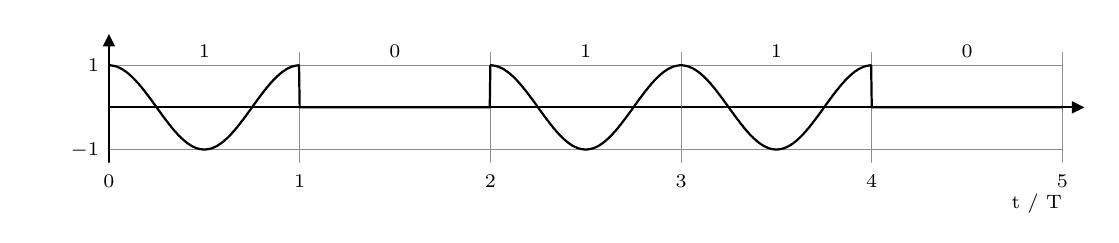
\begin{tikzpicture}[x=0.01985cm,y=-0.01985cm,line cap=round,line join=round]
\useasboundingbox (0,0) rectangle (680,120);
\path[draw=black!45,line width=0.35pt] (52,86) -- (52,16);
\path[draw=black!45,line width=0.35pt] (174,86) -- (174,16);
\path[draw=black!45,line width=0.35pt] (296,86) -- (296,16);
\path[draw=black!45,line width=0.35pt] (418,86) -- (418,16);
\path[draw=black!45,line width=0.35pt] (540,86) -- (540,16);
\path[draw=black!45,line width=0.35pt] (662,86) -- (662,16);
\path[draw=black!45,line width=0.35pt] (52,24.1) -- (662,24.1);
\path[draw=black!45,line width=0.35pt] (52,77.9) -- (662,77.9);
\path[draw=black,line width=0.7pt] (52,51) -- (670,51);
\path[fill=black,draw=none] (676,51) -- (668,47) -- (668,55) -- cycle;
\path[draw=black,line width=0.7pt] (52,86) -- (52,10);
\path[fill=black,draw=none] (52,4) -- (48,12) -- (56,12) -- cycle;
\node[anchor=base,inner sep=0pt,font=\scriptsize] at (52,102) {0};
\node[anchor=base,inner sep=0pt,font=\scriptsize] at (174,102) {1};
\node[anchor=base,inner sep=0pt,font=\scriptsize] at (296,102) {2};
\node[anchor=base,inner sep=0pt,font=\scriptsize] at (418,102) {3};
\node[anchor=base,inner sep=0pt,font=\scriptsize] at (540,102) {4};
\node[anchor=base,inner sep=0pt,font=\scriptsize] at (662,102) {5};
\node[anchor=base east,inner sep=0pt,font=\scriptsize] at (46,28.1) {1};
\node[anchor=base east,inner sep=0pt,font=\scriptsize] at (46,81.9) {$-$1};
\node[anchor=base east,inner sep=0pt,font=\scriptsize] at (662,116) {t / T};
\path[draw=black!45,line width=0.35pt,dash pattern=on 3pt off 2pt] (174,86) -- (174,16);
\path[draw=black!45,line width=0.35pt,dash pattern=on 3pt off 2pt] (296,86) -- (296,16);
\path[draw=black!45,line width=0.35pt,dash pattern=on 3pt off 2pt] (418,86) -- (418,16);
\path[draw=black!45,line width=0.35pt,dash pattern=on 3pt off 2pt] (540,86) -- (540,16);
\path[draw=black,line width=0.8pt] (52,24.1) -- (52.4,24.1) -- (52.8,24.1) -- (53.1,24.1) -- (53.5,24.2) -- (53.9,24.2) -- (54.3,24.3) -- (54.7,24.3) -- (55.1,24.4) -- (55.4,24.5) -- (55.8,24.6) -- (56.2,24.7) -- (56.6,24.8) -- (57,24.9) -- (57.3,25.1) -- (57.7,25.2) -- (58.1,25.4) -- (58.5,25.6) -- (58.9,25.7) -- (59.2,25.9) -- (59.6,26.1) -- (60,26.3) -- (60.4,26.5) -- (60.8,26.8) -- (61.2,27) -- (61.5,27.3) -- (61.9,27.5) -- (62.3,27.8) -- (62.7,28) -- (63.1,28.3) -- (63.4,28.6) -- (63.8,28.9) -- (64.2,29.2) -- (64.6,29.5) -- (65,29.9) -- (65.3,30.2) -- (65.7,30.5) -- (66.1,30.9) -- (66.5,31.2) -- (66.9,31.6) -- (67.3,32) -- (67.6,32.3) -- (68,32.7) -- (68.4,33.1) -- (68.8,33.5) -- (69.2,33.9) -- (69.5,34.3) -- (69.9,34.8) -- (70.3,35.2) -- (70.7,35.6) -- (71.1,36) -- (71.4,36.5) -- (71.8,36.9) -- (72.2,37.4) -- (72.6,37.8) -- (73,38.3) -- (73.4,38.8) -- (73.7,39.3) -- (74.1,39.7) -- (74.5,40.2) -- (74.9,40.7) -- (75.3,41.2) -- (75.6,41.7) -- (76,42.2) -- (76.4,42.7) -- (76.8,43.2) -- (77.2,43.7) -- (77.5,44.2) -- (77.9,44.7) -- (78.3,45.2) -- (78.7,45.7) -- (79.1,46.3) -- (79.5,46.8) -- (79.8,47.3) -- (80.2,47.8) -- (80.6,48.4) -- (81,48.9) -- (81.4,49.4) -- (81.7,49.9) -- (82.1,50.5) -- (82.5,51) -- (82.9,51.5) -- (83.3,52.1) -- (83.6,52.6) -- (84,53.1) -- (84.4,53.6) -- (84.8,54.2) -- (85.2,54.7) -- (85.6,55.2) -- (85.9,55.7) -- (86.3,56.3) -- (86.7,56.8) -- (87.1,57.3) -- (87.5,57.8) -- (87.8,58.3) -- (88.2,58.8) -- (88.6,59.3) -- (89,59.8) -- (89.4,60.3) -- (89.7,60.8) -- (90.1,61.3) -- (90.5,61.8) -- (90.9,62.3) -- (91.3,62.7) -- (91.7,63.2) -- (92,63.7) -- (92.4,64.2) -- (92.8,64.6) -- (93.2,65.1) -- (93.6,65.5) -- (93.9,66) -- (94.3,66.4) -- (94.7,66.8) -- (95.1,67.2) -- (95.5,67.7) -- (95.8,68.1) -- (96.2,68.5) -- (96.6,68.9) -- (97,69.3) -- (97.4,69.7) -- (97.8,70) -- (98.1,70.4) -- (98.5,70.8) -- (98.9,71.1) -- (99.3,71.5) -- (99.7,71.8) -- (100,72.1) -- (100.4,72.5) -- (100.8,72.8) -- (101.2,73.1) -- (101.6,73.4) -- (101.9,73.7) -- (102.3,74) -- (102.7,74.2) -- (103.1,74.5) -- (103.5,74.7) -- (103.9,75) -- (104.2,75.2) -- (104.6,75.5) -- (105,75.7) -- (105.4,75.9) -- (105.8,76.1) -- (106.1,76.3) -- (106.5,76.4) -- (106.9,76.6) -- (107.3,76.8) -- (107.7,76.9) -- (108,77.1) -- (108.4,77.2) -- (108.8,77.3) -- (109.2,77.4) -- (109.6,77.5) -- (110,77.6) -- (110.3,77.7) -- (110.7,77.7) -- (111.1,77.8) -- (111.5,77.8) -- (111.9,77.9) -- (112.2,77.9) -- (112.6,77.9) -- (113,77.9) -- (113.4,77.9) -- (113.8,77.9) -- (114.1,77.9) -- (114.5,77.8) -- (114.9,77.8) -- (115.3,77.7) -- (115.7,77.7) -- (116.1,77.6) -- (116.4,77.5) -- (116.8,77.4) -- (117.2,77.3) -- (117.6,77.2) -- (118,77.1) -- (118.3,76.9) -- (118.7,76.8) -- (119.1,76.6) -- (119.5,76.4) -- (119.9,76.3) -- (120.2,76.1) -- (120.6,75.9) -- (121,75.7) -- (121.4,75.5) -- (121.8,75.2) -- (122.2,75) -- (122.5,74.7) -- (122.9,74.5) -- (123.3,74.2) -- (123.7,74) -- (124.1,73.7) -- (124.4,73.4) -- (124.8,73.1) -- (125.2,72.8) -- (125.6,72.5) -- (126,72.1) -- (126.3,71.8) -- (126.7,71.5) -- (127.1,71.1) -- (127.5,70.8) -- (127.9,70.4) -- (128.3,70) -- (128.6,69.7) -- (129,69.3) -- (129.4,68.9) -- (129.8,68.5) -- (130.2,68.1) -- (130.5,67.7) -- (130.9,67.2) -- (131.3,66.8) -- (131.7,66.4) -- (132.1,66) -- (132.4,65.5) -- (132.8,65.1) -- (133.2,64.6) -- (133.6,64.2) -- (134,63.7) -- (134.4,63.2) -- (134.7,62.7) -- (135.1,62.3) -- (135.5,61.8) -- (135.9,61.3) -- (136.3,60.8) -- (136.6,60.3) -- (137,59.8) -- (137.4,59.3) -- (137.8,58.8) -- (138.2,58.3) -- (138.5,57.8) -- (138.9,57.3) -- (139.3,56.8) -- (139.7,56.3) -- (140.1,55.7) -- (140.5,55.2) -- (140.8,54.7) -- (141.2,54.2) -- (141.6,53.6) -- (142,53.1) -- (142.4,52.6) -- (142.7,52.1) -- (143.1,51.5) -- (143.5,51) -- (143.9,50.5) -- (144.3,49.9) -- (144.6,49.4) -- (145,48.9) -- (145.4,48.4) -- (145.8,47.8) -- (146.2,47.3) -- (146.6,46.8) -- (146.9,46.3) -- (147.3,45.7) -- (147.7,45.2) -- (148.1,44.7) -- (148.5,44.2) -- (148.8,43.7) -- (149.2,43.2) -- (149.6,42.7) -- (150,42.2) -- (150.4,41.7) -- (150.7,41.2) -- (151.1,40.7) -- (151.5,40.2) -- (151.9,39.7) -- (152.3,39.3) -- (152.6,38.8) -- (153,38.3) -- (153.4,37.8) -- (153.8,37.4) -- (154.2,36.9) -- (154.6,36.5) -- (154.9,36) -- (155.3,35.6) -- (155.7,35.2) -- (156.1,34.8) -- (156.5,34.3) -- (156.8,33.9) -- (157.2,33.5) -- (157.6,33.1) -- (158,32.7) -- (158.4,32.3) -- (158.8,32) -- (159.1,31.6) -- (159.5,31.2) -- (159.9,30.9) -- (160.3,30.5) -- (160.7,30.2) -- (161,29.9) -- (161.4,29.5) -- (161.8,29.2) -- (162.2,28.9) -- (162.6,28.6) -- (162.9,28.3) -- (163.3,28) -- (163.7,27.8) -- (164.1,27.5) -- (164.5,27.3) -- (164.9,27) -- (165.2,26.8) -- (165.6,26.5) -- (166,26.3) -- (166.4,26.1) -- (166.8,25.9) -- (167.1,25.7) -- (167.5,25.6) -- (167.9,25.4) -- (168.3,25.2) -- (168.7,25.1) -- (169,24.9) -- (169.4,24.8) -- (169.8,24.7) -- (170.2,24.6) -- (170.6,24.5) -- (171,24.4) -- (171.3,24.3) -- (171.7,24.3) -- (172.1,24.2) -- (172.5,24.2) -- (172.9,24.1) -- (173.2,24.1) -- (173.6,24.1) -- (174,51) -- (174.4,51) -- (174.8,51) -- (175.1,51) -- (175.5,51) -- (175.9,51) -- (176.3,51) -- (176.7,51) -- (177.1,51) -- (177.4,51) -- (177.8,51) -- (178.2,51) -- (178.6,51) -- (179,51) -- (179.3,51) -- (179.7,51) -- (180.1,51) -- (180.5,51) -- (180.9,51) -- (181.2,51) -- (181.6,51) -- (182,51) -- (182.4,51) -- (182.8,51) -- (183.2,51) -- (183.5,51) -- (183.9,51) -- (184.3,51) -- (184.7,51) -- (185.1,51) -- (185.4,51) -- (185.8,51) -- (186.2,51) -- (186.6,51) -- (187,51) -- (187.3,51) -- (187.7,51) -- (188.1,51) -- (188.5,51) -- (188.9,51) -- (189.3,51) -- (189.6,51) -- (190,51) -- (190.4,51) -- (190.8,51) -- (191.2,51) -- (191.5,51) -- (191.9,51) -- (192.3,51) -- (192.7,51) -- (193.1,51) -- (193.4,51) -- (193.8,51) -- (194.2,51) -- (194.6,51) -- (195,51) -- (195.4,51) -- (195.7,51) -- (196.1,51) -- (196.5,51) -- (196.9,51) -- (197.3,51) -- (197.6,51) -- (198,51) -- (198.4,51) -- (198.8,51) -- (199.2,51) -- (199.5,51) -- (199.9,51) -- (200.3,51) -- (200.7,51) -- (201.1,51) -- (201.5,51) -- (201.8,51) -- (202.2,51) -- (202.6,51) -- (203,51) -- (203.4,51) -- (203.7,51) -- (204.1,51) -- (204.5,51) -- (204.9,51) -- (205.3,51) -- (205.6,51) -- (206,51) -- (206.4,51) -- (206.8,51) -- (207.2,51) -- (207.6,51) -- (207.9,51) -- (208.3,51) -- (208.7,51) -- (209.1,51) -- (209.5,51) -- (209.8,51) -- (210.2,51) -- (210.6,51) -- (211,51) -- (211.4,51) -- (211.7,51) -- (212.1,51) -- (212.5,51) -- (212.9,51) -- (213.3,51) -- (213.7,51) -- (214,51) -- (214.4,51) -- (214.8,51) -- (215.2,51) -- (215.6,51) -- (215.9,51) -- (216.3,51) -- (216.7,51) -- (217.1,51) -- (217.5,51) -- (217.8,51) -- (218.2,51) -- (218.6,51) -- (219,51) -- (219.4,51) -- (219.8,51) -- (220.1,51) -- (220.5,51) -- (220.9,51) -- (221.3,51) -- (221.7,51) -- (222,51) -- (222.4,51) -- (222.8,51) -- (223.2,51) -- (223.6,51) -- (223.9,51) -- (224.3,51) -- (224.7,51) -- (225.1,51) -- (225.5,51) -- (225.9,51) -- (226.2,51) -- (226.6,51) -- (227,51) -- (227.4,51) -- (227.8,51) -- (228.1,51) -- (228.5,51) -- (228.9,51) -- (229.3,51) -- (229.7,51) -- (230,51) -- (230.4,51) -- (230.8,51) -- (231.2,51) -- (231.6,51) -- (232,51) -- (232.3,51) -- (232.7,51) -- (233.1,51) -- (233.5,51) -- (233.9,51) -- (234.2,51) -- (234.6,51) -- (235,51) -- (235.4,51) -- (235.8,51) -- (236.1,51) -- (236.5,51) -- (236.9,51) -- (237.3,51) -- (237.7,51) -- (238.1,51) -- (238.4,51) -- (238.8,51) -- (239.2,51) -- (239.6,51) -- (240,51) -- (240.3,51) -- (240.7,51) -- (241.1,51) -- (241.5,51) -- (241.9,51) -- (242.2,51) -- (242.6,51) -- (243,51) -- (243.4,51) -- (243.8,51) -- (244.2,51) -- (244.5,51) -- (244.9,51) -- (245.3,51) -- (245.7,51) -- (246.1,51) -- (246.4,51) -- (246.8,51) -- (247.2,51) -- (247.6,51) -- (248,51) -- (248.3,51) -- (248.7,51) -- (249.1,51) -- (249.5,51) -- (249.9,51) -- (250.3,51) -- (250.6,51) -- (251,51) -- (251.4,51) -- (251.8,51) -- (252.2,51) -- (252.5,51) -- (252.9,51) -- (253.3,51) -- (253.7,51) -- (254.1,51) -- (254.4,51) -- (254.8,51) -- (255.2,51) -- (255.6,51) -- (256,51) -- (256.4,51) -- (256.7,51) -- (257.1,51) -- (257.5,51) -- (257.9,51) -- (258.3,51) -- (258.6,51) -- (259,51) -- (259.4,51) -- (259.8,51) -- (260.2,51) -- (260.5,51) -- (260.9,51) -- (261.3,51) -- (261.7,51) -- (262.1,51) -- (262.5,51) -- (262.8,51) -- (263.2,51) -- (263.6,51) -- (264,51) -- (264.4,51) -- (264.7,51) -- (265.1,51) -- (265.5,51) -- (265.9,51) -- (266.3,51) -- (266.6,51) -- (267,51) -- (267.4,51) -- (267.8,51) -- (268.2,51) -- (268.5,51) -- (268.9,51) -- (269.3,51) -- (269.7,51) -- (270.1,51) -- (270.5,51) -- (270.8,51) -- (271.2,51) -- (271.6,51) -- (272,51) -- (272.4,51) -- (272.7,51) -- (273.1,51) -- (273.5,51) -- (273.9,51) -- (274.3,51) -- (274.7,51) -- (275,51) -- (275.4,51) -- (275.8,51) -- (276.2,51) -- (276.6,51) -- (276.9,51) -- (277.3,51) -- (277.7,51) -- (278.1,51) -- (278.5,51) -- (278.8,51) -- (279.2,51) -- (279.6,51) -- (280,51) -- (280.4,51) -- (280.8,51) -- (281.1,51) -- (281.5,51) -- (281.9,51) -- (282.3,51) -- (282.7,51) -- (283,51) -- (283.4,51) -- (283.8,51) -- (284.2,51) -- (284.6,51) -- (284.9,51) -- (285.3,51) -- (285.7,51) -- (286.1,51) -- (286.5,51) -- (286.9,51) -- (287.2,51) -- (287.6,51) -- (288,51) -- (288.4,51) -- (288.8,51) -- (289.1,51) -- (289.5,51) -- (289.9,51) -- (290.3,51) -- (290.7,51) -- (291,51) -- (291.4,51) -- (291.8,51) -- (292.2,51) -- (292.6,51) -- (293,51) -- (293.3,51) -- (293.7,51) -- (294.1,51) -- (294.5,51) -- (294.9,51) -- (295.2,51) -- (295.6,51) -- (296,24.1) -- (296.4,24.1) -- (296.8,24.1) -- (297.1,24.1) -- (297.5,24.2) -- (297.9,24.2) -- (298.3,24.3) -- (298.7,24.3) -- (299,24.4) -- (299.4,24.5) -- (299.8,24.6) -- (300.2,24.7) -- (300.6,24.8) -- (301,24.9) -- (301.3,25.1) -- (301.7,25.2) -- (302.1,25.4) -- (302.5,25.6) -- (302.9,25.7) -- (303.2,25.9) -- (303.6,26.1) -- (304,26.3) -- (304.4,26.5) -- (304.8,26.8) -- (305.2,27) -- (305.5,27.3) -- (305.9,27.5) -- (306.3,27.8) -- (306.7,28) -- (307.1,28.3) -- (307.4,28.6) -- (307.8,28.9) -- (308.2,29.2) -- (308.6,29.5) -- (309,29.9) -- (309.3,30.2) -- (309.7,30.5) -- (310.1,30.9) -- (310.5,31.2) -- (310.9,31.6) -- (311.3,32) -- (311.6,32.3) -- (312,32.7) -- (312.4,33.1) -- (312.8,33.5) -- (313.2,33.9) -- (313.5,34.3) -- (313.9,34.8) -- (314.3,35.2) -- (314.7,35.6) -- (315.1,36) -- (315.4,36.5) -- (315.8,36.9) -- (316.2,37.4) -- (316.6,37.8) -- (317,38.3) -- (317.3,38.8) -- (317.7,39.3) -- (318.1,39.7) -- (318.5,40.2) -- (318.9,40.7) -- (319.3,41.2) -- (319.6,41.7) -- (320,42.2) -- (320.4,42.7) -- (320.8,43.2) -- (321.2,43.7) -- (321.5,44.2) -- (321.9,44.7) -- (322.3,45.2) -- (322.7,45.7) -- (323.1,46.3) -- (323.5,46.8) -- (323.8,47.3) -- (324.2,47.8) -- (324.6,48.4) -- (325,48.9) -- (325.4,49.4) -- (325.7,49.9) -- (326.1,50.5) -- (326.5,51) -- (326.9,51.5) -- (327.3,52.1) -- (327.6,52.6) -- (328,53.1) -- (328.4,53.6) -- (328.8,54.2) -- (329.2,54.7) -- (329.5,55.2) -- (329.9,55.7) -- (330.3,56.3) -- (330.7,56.8) -- (331.1,57.3) -- (331.5,57.8) -- (331.8,58.3) -- (332.2,58.8) -- (332.6,59.3) -- (333,59.8) -- (333.4,60.3) -- (333.7,60.8) -- (334.1,61.3) -- (334.5,61.8) -- (334.9,62.3) -- (335.3,62.7) -- (335.7,63.2) -- (336,63.7) -- (336.4,64.2) -- (336.8,64.6) -- (337.2,65.1) -- (337.6,65.5) -- (337.9,66) -- (338.3,66.4) -- (338.7,66.8) -- (339.1,67.2) -- (339.5,67.7) -- (339.8,68.1) -- (340.2,68.5) -- (340.6,68.9) -- (341,69.3) -- (341.4,69.7) -- (341.8,70) -- (342.1,70.4) -- (342.5,70.8) -- (342.9,71.1) -- (343.3,71.5) -- (343.7,71.8) -- (344,72.1) -- (344.4,72.5) -- (344.8,72.8) -- (345.2,73.1) -- (345.6,73.4) -- (345.9,73.7) -- (346.3,74) -- (346.7,74.2) -- (347.1,74.5) -- (347.5,74.7) -- (347.8,75) -- (348.2,75.2) -- (348.6,75.5) -- (349,75.7) -- (349.4,75.9) -- (349.8,76.1) -- (350.1,76.3) -- (350.5,76.4) -- (350.9,76.6) -- (351.3,76.8) -- (351.7,76.9) -- (352,77.1) -- (352.4,77.2) -- (352.8,77.3) -- (353.2,77.4) -- (353.6,77.5) -- (354,77.6) -- (354.3,77.7) -- (354.7,77.7) -- (355.1,77.8) -- (355.5,77.8) -- (355.9,77.9) -- (356.2,77.9) -- (356.6,77.9) -- (357,77.9) -- (357.4,77.9) -- (357.8,77.9) -- (358.1,77.9) -- (358.5,77.8) -- (358.9,77.8) -- (359.3,77.7) -- (359.7,77.7) -- (360.1,77.6) -- (360.4,77.5) -- (360.8,77.4) -- (361.2,77.3) -- (361.6,77.2) -- (362,77.1) -- (362.3,76.9) -- (362.7,76.8) -- (363.1,76.6) -- (363.5,76.4) -- (363.9,76.3) -- (364.2,76.1) -- (364.6,75.9) -- (365,75.7) -- (365.4,75.5) -- (365.8,75.2) -- (366.2,75) -- (366.5,74.7) -- (366.9,74.5) -- (367.3,74.2) -- (367.7,74) -- (368.1,73.7) -- (368.4,73.4) -- (368.8,73.1) -- (369.2,72.8) -- (369.6,72.5) -- (370,72.1) -- (370.3,71.8) -- (370.7,71.5) -- (371.1,71.1) -- (371.5,70.8) -- (371.9,70.4) -- (372.3,70) -- (372.6,69.7) -- (373,69.3) -- (373.4,68.9) -- (373.8,68.5) -- (374.2,68.1) -- (374.5,67.7) -- (374.9,67.2) -- (375.3,66.8) -- (375.7,66.4) -- (376.1,66) -- (376.4,65.5) -- (376.8,65.1) -- (377.2,64.6) -- (377.6,64.2) -- (378,63.7) -- (378.3,63.2) -- (378.7,62.7) -- (379.1,62.3) -- (379.5,61.8) -- (379.9,61.3) -- (380.3,60.8) -- (380.6,60.3) -- (381,59.8) -- (381.4,59.3) -- (381.8,58.8) -- (382.2,58.3) -- (382.5,57.8) -- (382.9,57.3) -- (383.3,56.8) -- (383.7,56.3) -- (384.1,55.7) -- (384.5,55.2) -- (384.8,54.7) -- (385.2,54.2) -- (385.6,53.6) -- (386,53.1) -- (386.4,52.6) -- (386.7,52.1) -- (387.1,51.5) -- (387.5,51) -- (387.9,50.5) -- (388.3,49.9) -- (388.6,49.4) -- (389,48.9) -- (389.4,48.4) -- (389.8,47.8) -- (390.2,47.3) -- (390.5,46.8) -- (390.9,46.3) -- (391.3,45.7) -- (391.7,45.2) -- (392.1,44.7) -- (392.5,44.2) -- (392.8,43.7) -- (393.2,43.2) -- (393.6,42.7) -- (394,42.2) -- (394.4,41.7) -- (394.7,41.2) -- (395.1,40.7) -- (395.5,40.2) -- (395.9,39.7) -- (396.3,39.3) -- (396.7,38.8) -- (397,38.3) -- (397.4,37.8) -- (397.8,37.4) -- (398.2,36.9) -- (398.6,36.5) -- (398.9,36) -- (399.3,35.6) -- (399.7,35.2) -- (400.1,34.8) -- (400.5,34.3) -- (400.8,33.9) -- (401.2,33.5) -- (401.6,33.1) -- (402,32.7) -- (402.4,32.3) -- (402.8,32) -- (403.1,31.6) -- (403.5,31.2) -- (403.9,30.9) -- (404.3,30.5) -- (404.7,30.2) -- (405,29.9) -- (405.4,29.5) -- (405.8,29.2) -- (406.2,28.9) -- (406.6,28.6) -- (406.9,28.3) -- (407.3,28) -- (407.7,27.8) -- (408.1,27.5) -- (408.5,27.3) -- (408.8,27) -- (409.2,26.8) -- (409.6,26.5) -- (410,26.3) -- (410.4,26.1) -- (410.8,25.9) -- (411.1,25.7) -- (411.5,25.6) -- (411.9,25.4) -- (412.3,25.2) -- (412.7,25.1) -- (413,24.9) -- (413.4,24.8) -- (413.8,24.7) -- (414.2,24.6) -- (414.6,24.5) -- (415,24.4) -- (415.3,24.3) -- (415.7,24.3) -- (416.1,24.2) -- (416.5,24.2) -- (416.9,24.1) -- (417.2,24.1) -- (417.6,24.1) -- (418,24.1) -- (418.4,24.1) -- (418.8,24.1) -- (419.1,24.1) -- (419.5,24.2) -- (419.9,24.2) -- (420.3,24.3) -- (420.7,24.3) -- (421.1,24.4) -- (421.4,24.5) -- (421.8,24.6) -- (422.2,24.7) -- (422.6,24.8) -- (423,24.9) -- (423.3,25.1) -- (423.7,25.2) -- (424.1,25.4) -- (424.5,25.6) -- (424.9,25.7) -- (425.2,25.9) -- (425.6,26.1) -- (426,26.3) -- (426.4,26.5) -- (426.8,26.8) -- (427.2,27) -- (427.5,27.3) -- (427.9,27.5) -- (428.3,27.8) -- (428.7,28) -- (429.1,28.3) -- (429.4,28.6) -- (429.8,28.9) -- (430.2,29.2) -- (430.6,29.5) -- (431,29.9) -- (431.3,30.2) -- (431.7,30.5) -- (432.1,30.9) -- (432.5,31.2) -- (432.9,31.6) -- (433.3,32) -- (433.6,32.3) -- (434,32.7) -- (434.4,33.1) -- (434.8,33.5) -- (435.2,33.9) -- (435.5,34.3) -- (435.9,34.8) -- (436.3,35.2) -- (436.7,35.6) -- (437.1,36) -- (437.4,36.5) -- (437.8,36.9) -- (438.2,37.4) -- (438.6,37.8) -- (439,38.3) -- (439.4,38.8) -- (439.7,39.3) -- (440.1,39.7) -- (440.5,40.2) -- (440.9,40.7) -- (441.3,41.2) -- (441.6,41.7) -- (442,42.2) -- (442.4,42.7) -- (442.8,43.2) -- (443.2,43.7) -- (443.5,44.2) -- (443.9,44.7) -- (444.3,45.2) -- (444.7,45.7) -- (445.1,46.3) -- (445.5,46.8) -- (445.8,47.3) -- (446.2,47.8) -- (446.6,48.4) -- (447,48.9) -- (447.4,49.4) -- (447.7,49.9) -- (448.1,50.5) -- (448.5,51) -- (448.9,51.5) -- (449.3,52.1) -- (449.6,52.6) -- (450,53.1) -- (450.4,53.6) -- (450.8,54.2) -- (451.2,54.7) -- (451.6,55.2) -- (451.9,55.7) -- (452.3,56.3) -- (452.7,56.8) -- (453.1,57.3) -- (453.5,57.8) -- (453.8,58.3) -- (454.2,58.8) -- (454.6,59.3) -- (455,59.8) -- (455.4,60.3) -- (455.7,60.8) -- (456.1,61.3) -- (456.5,61.8) -- (456.9,62.3) -- (457.3,62.7) -- (457.7,63.2) -- (458,63.7) -- (458.4,64.2) -- (458.8,64.6) -- (459.2,65.1) -- (459.6,65.5) -- (459.9,66) -- (460.3,66.4) -- (460.7,66.8) -- (461.1,67.2) -- (461.5,67.7) -- (461.8,68.1) -- (462.2,68.5) -- (462.6,68.9) -- (463,69.3) -- (463.4,69.7) -- (463.8,70) -- (464.1,70.4) -- (464.5,70.8) -- (464.9,71.1) -- (465.3,71.5) -- (465.7,71.8) -- (466,72.1) -- (466.4,72.5) -- (466.8,72.8) -- (467.2,73.1) -- (467.6,73.4) -- (467.9,73.7) -- (468.3,74) -- (468.7,74.2) -- (469.1,74.5) -- (469.5,74.7) -- (469.9,75) -- (470.2,75.2) -- (470.6,75.5) -- (471,75.7) -- (471.4,75.9) -- (471.8,76.1) -- (472.1,76.3) -- (472.5,76.4) -- (472.9,76.6) -- (473.3,76.8) -- (473.7,76.9) -- (474,77.1) -- (474.4,77.2) -- (474.8,77.3) -- (475.2,77.4) -- (475.6,77.5) -- (476,77.6) -- (476.3,77.7) -- (476.7,77.7) -- (477.1,77.8) -- (477.5,77.8) -- (477.9,77.9) -- (478.2,77.9) -- (478.6,77.9) -- (479,77.9) -- (479.4,77.9) -- (479.8,77.9) -- (480.1,77.9) -- (480.5,77.8) -- (480.9,77.8) -- (481.3,77.7) -- (481.7,77.7) -- (482.1,77.6) -- (482.4,77.5) -- (482.8,77.4) -- (483.2,77.3) -- (483.6,77.2) -- (484,77.1) -- (484.3,76.9) -- (484.7,76.8) -- (485.1,76.6) -- (485.5,76.4) -- (485.9,76.3) -- (486.2,76.1) -- (486.6,75.9) -- (487,75.7) -- (487.4,75.5) -- (487.8,75.2) -- (488.2,75) -- (488.5,74.7) -- (488.9,74.5) -- (489.3,74.2) -- (489.7,74) -- (490.1,73.7) -- (490.4,73.4) -- (490.8,73.1) -- (491.2,72.8) -- (491.6,72.5) -- (492,72.1) -- (492.3,71.8) -- (492.7,71.5) -- (493.1,71.1) -- (493.5,70.8) -- (493.9,70.4) -- (494.3,70) -- (494.6,69.7) -- (495,69.3) -- (495.4,68.9) -- (495.8,68.5) -- (496.2,68.1) -- (496.5,67.7) -- (496.9,67.2) -- (497.3,66.8) -- (497.7,66.4) -- (498.1,66) -- (498.4,65.5) -- (498.8,65.1) -- (499.2,64.6) -- (499.6,64.2) -- (500,63.7) -- (500.4,63.2) -- (500.7,62.7) -- (501.1,62.3) -- (501.5,61.8) -- (501.9,61.3) -- (502.3,60.8) -- (502.6,60.3) -- (503,59.8) -- (503.4,59.3) -- (503.8,58.8) -- (504.2,58.3) -- (504.5,57.8) -- (504.9,57.3) -- (505.3,56.8) -- (505.7,56.3) -- (506.1,55.7) -- (506.5,55.2) -- (506.8,54.7) -- (507.2,54.2) -- (507.6,53.6) -- (508,53.1) -- (508.4,52.6) -- (508.7,52.1) -- (509.1,51.5) -- (509.5,51) -- (509.9,50.5) -- (510.3,49.9) -- (510.6,49.4) -- (511,48.9) -- (511.4,48.4) -- (511.8,47.8) -- (512.2,47.3) -- (512.6,46.8) -- (512.9,46.3) -- (513.3,45.7) -- (513.7,45.2) -- (514.1,44.7) -- (514.5,44.2) -- (514.8,43.7) -- (515.2,43.2) -- (515.6,42.7) -- (516,42.2) -- (516.4,41.7) -- (516.7,41.2) -- (517.1,40.7) -- (517.5,40.2) -- (517.9,39.7) -- (518.3,39.3) -- (518.7,38.8) -- (519,38.3) -- (519.4,37.8) -- (519.8,37.4) -- (520.2,36.9) -- (520.6,36.5) -- (520.9,36) -- (521.3,35.6) -- (521.7,35.2) -- (522.1,34.8) -- (522.5,34.3) -- (522.8,33.9) -- (523.2,33.5) -- (523.6,33.1) -- (524,32.7) -- (524.4,32.3) -- (524.8,32) -- (525.1,31.6) -- (525.5,31.2) -- (525.9,30.9) -- (526.3,30.5) -- (526.7,30.2) -- (527,29.9) -- (527.4,29.5) -- (527.8,29.2) -- (528.2,28.9) -- (528.6,28.6) -- (528.9,28.3) -- (529.3,28) -- (529.7,27.8) -- (530.1,27.5) -- (530.5,27.3) -- (530.8,27) -- (531.2,26.8) -- (531.6,26.5) -- (532,26.3) -- (532.4,26.1) -- (532.8,25.9) -- (533.1,25.7) -- (533.5,25.6) -- (533.9,25.4) -- (534.3,25.2) -- (534.7,25.1) -- (535,24.9) -- (535.4,24.8) -- (535.8,24.7) -- (536.2,24.6) -- (536.6,24.5) -- (537,24.4) -- (537.3,24.3) -- (537.7,24.3) -- (538.1,24.2) -- (538.5,24.2) -- (538.9,24.1) -- (539.2,24.1) -- (539.6,24.1) -- (540,51) -- (540.4,51) -- (540.8,51) -- (541.1,51) -- (541.5,51) -- (541.9,51) -- (542.3,51) -- (542.7,51) -- (543.1,51) -- (543.4,51) -- (543.8,51) -- (544.2,51) -- (544.6,51) -- (545,51) -- (545.3,51) -- (545.7,51) -- (546.1,51) -- (546.5,51) -- (546.9,51) -- (547.2,51) -- (547.6,51) -- (548,51) -- (548.4,51) -- (548.8,51) -- (549.2,51) -- (549.5,51) -- (549.9,51) -- (550.3,51) -- (550.7,51) -- (551.1,51) -- (551.4,51) -- (551.8,51) -- (552.2,51) -- (552.6,51) -- (553,51) -- (553.3,51) -- (553.7,51) -- (554.1,51) -- (554.5,51) -- (554.9,51) -- (555.3,51) -- (555.6,51) -- (556,51) -- (556.4,51) -- (556.8,51) -- (557.2,51) -- (557.5,51) -- (557.9,51) -- (558.3,51) -- (558.7,51) -- (559.1,51) -- (559.4,51) -- (559.8,51) -- (560.2,51) -- (560.6,51) -- (561,51) -- (561.3,51) -- (561.7,51) -- (562.1,51) -- (562.5,51) -- (562.9,51) -- (563.3,51) -- (563.6,51) -- (564,51) -- (564.4,51) -- (564.8,51) -- (565.2,51) -- (565.5,51) -- (565.9,51) -- (566.3,51) -- (566.7,51) -- (567.1,51) -- (567.4,51) -- (567.8,51) -- (568.2,51) -- (568.6,51) -- (569,51) -- (569.4,51) -- (569.7,51) -- (570.1,51) -- (570.5,51) -- (570.9,51) -- (571.3,51) -- (571.6,51) -- (572,51) -- (572.4,51) -- (572.8,51) -- (573.2,51) -- (573.6,51) -- (573.9,51) -- (574.3,51) -- (574.7,51) -- (575.1,51) -- (575.5,51) -- (575.8,51) -- (576.2,51) -- (576.6,51) -- (577,51) -- (577.4,51) -- (577.7,51) -- (578.1,51) -- (578.5,51) -- (578.9,51) -- (579.3,51) -- (579.7,51) -- (580,51) -- (580.4,51) -- (580.8,51) -- (581.2,51) -- (581.6,51) -- (581.9,51) -- (582.3,51) -- (582.7,51) -- (583.1,51) -- (583.5,51) -- (583.8,51) -- (584.2,51) -- (584.6,51) -- (585,51) -- (585.4,51) -- (585.8,51) -- (586.1,51) -- (586.5,51) -- (586.9,51) -- (587.3,51) -- (587.7,51) -- (588,51) -- (588.4,51) -- (588.8,51) -- (589.2,51) -- (589.6,51) -- (589.9,51) -- (590.3,51) -- (590.7,51) -- (591.1,51) -- (591.5,51) -- (591.9,51) -- (592.2,51) -- (592.6,51) -- (593,51) -- (593.4,51) -- (593.8,51) -- (594.1,51) -- (594.5,51) -- (594.9,51) -- (595.3,51) -- (595.7,51) -- (596,51) -- (596.4,51) -- (596.8,51) -- (597.2,51) -- (597.6,51) -- (597.9,51) -- (598.3,51) -- (598.7,51) -- (599.1,51) -- (599.5,51) -- (599.9,51) -- (600.2,51) -- (600.6,51) -- (601,51) -- (601.4,51) -- (601.8,51) -- (602.1,51) -- (602.5,51) -- (602.9,51) -- (603.3,51) -- (603.7,51) -- (604.1,51) -- (604.4,51) -- (604.8,51) -- (605.2,51) -- (605.6,51) -- (606,51) -- (606.3,51) -- (606.7,51) -- (607.1,51) -- (607.5,51) -- (607.9,51) -- (608.2,51) -- (608.6,51) -- (609,51) -- (609.4,51) -- (609.8,51) -- (610.2,51) -- (610.5,51) -- (610.9,51) -- (611.3,51) -- (611.7,51) -- (612.1,51) -- (612.4,51) -- (612.8,51) -- (613.2,51) -- (613.6,51) -- (614,51) -- (614.3,51) -- (614.7,51) -- (615.1,51) -- (615.5,51) -- (615.9,51) -- (616.3,51) -- (616.6,51) -- (617,51) -- (617.4,51) -- (617.8,51) -- (618.2,51) -- (618.5,51) -- (618.9,51) -- (619.3,51) -- (619.7,51) -- (620.1,51) -- (620.4,51) -- (620.8,51) -- (621.2,51) -- (621.6,51) -- (622,51) -- (622.3,51) -- (622.7,51) -- (623.1,51) -- (623.5,51) -- (623.9,51) -- (624.3,51) -- (624.6,51) -- (625,51) -- (625.4,51) -- (625.8,51) -- (626.2,51) -- (626.5,51) -- (626.9,51) -- (627.3,51) -- (627.7,51) -- (628.1,51) -- (628.4,51) -- (628.8,51) -- (629.2,51) -- (629.6,51) -- (630,51) -- (630.4,51) -- (630.7,51) -- (631.1,51) -- (631.5,51) -- (631.9,51) -- (632.3,51) -- (632.6,51) -- (633,51) -- (633.4,51) -- (633.8,51) -- (634.2,51) -- (634.6,51) -- (634.9,51) -- (635.3,51) -- (635.7,51) -- (636.1,51) -- (636.5,51) -- (636.8,51) -- (637.2,51) -- (637.6,51) -- (638,51) -- (638.4,51) -- (638.7,51) -- (639.1,51) -- (639.5,51) -- (639.9,51) -- (640.3,51) -- (640.7,51) -- (641,51) -- (641.4,51) -- (641.8,51) -- (642.2,51) -- (642.6,51) -- (642.9,51) -- (643.3,51) -- (643.7,51) -- (644.1,51) -- (644.5,51) -- (644.8,51) -- (645.2,51) -- (645.6,51) -- (646,51) -- (646.4,51) -- (646.8,51) -- (647.1,51) -- (647.5,51) -- (647.9,51) -- (648.3,51) -- (648.7,51) -- (649,51) -- (649.4,51) -- (649.8,51) -- (650.2,51) -- (650.6,51) -- (650.9,51) -- (651.3,51) -- (651.7,51) -- (652.1,51) -- (652.5,51) -- (652.9,51) -- (653.2,51) -- (653.6,51) -- (654,51) -- (654.4,51) -- (654.8,51) -- (655.1,51) -- (655.5,51) -- (655.9,51) -- (656.3,51) -- (656.7,51) -- (657,51) -- (657.4,51) -- (657.8,51) -- (658.2,51) -- (658.6,51) -- (658.9,51) -- (659.3,51) -- (659.7,51) -- (660.1,51) -- (660.5,51) -- (660.9,51) -- (661.2,51) -- (661.6,51) -- (662,51);
\node[anchor=base,inner sep=0pt,font=\scriptsize] at (113,18.8) {1};
\node[anchor=base,inner sep=0pt,font=\scriptsize] at (235,18.8) {0};
\node[anchor=base,inner sep=0pt,font=\scriptsize] at (357,18.8) {1};
\node[anchor=base,inner sep=0pt,font=\scriptsize] at (479,18.8) {1};
\node[anchor=base,inner sep=0pt,font=\scriptsize] at (601,18.8) {0};
\end{tikzpicture}\end{center}

\textbf{BPSK}\par
\begin{center}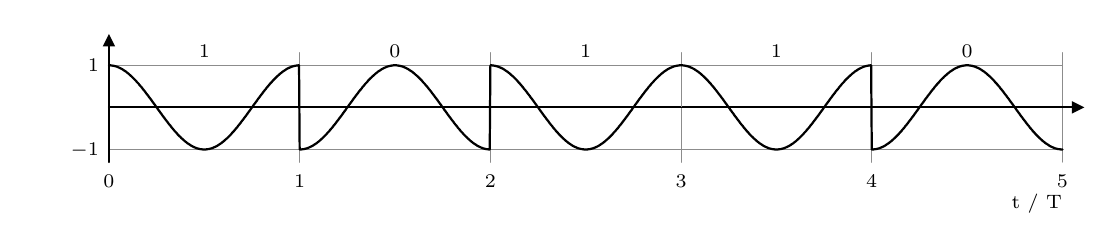
\begin{tikzpicture}[x=0.01985cm,y=-0.01985cm,line cap=round,line join=round]
\useasboundingbox (0,0) rectangle (680,120);
\path[draw=black!45,line width=0.35pt] (52,86) -- (52,16);
\path[draw=black!45,line width=0.35pt] (174,86) -- (174,16);
\path[draw=black!45,line width=0.35pt] (296,86) -- (296,16);
\path[draw=black!45,line width=0.35pt] (418,86) -- (418,16);
\path[draw=black!45,line width=0.35pt] (540,86) -- (540,16);
\path[draw=black!45,line width=0.35pt] (662,86) -- (662,16);
\path[draw=black!45,line width=0.35pt] (52,24.1) -- (662,24.1);
\path[draw=black!45,line width=0.35pt] (52,77.9) -- (662,77.9);
\path[draw=black,line width=0.7pt] (52,51) -- (670,51);
\path[fill=black,draw=none] (676,51) -- (668,47) -- (668,55) -- cycle;
\path[draw=black,line width=0.7pt] (52,86) -- (52,10);
\path[fill=black,draw=none] (52,4) -- (48,12) -- (56,12) -- cycle;
\node[anchor=base,inner sep=0pt,font=\scriptsize] at (52,102) {0};
\node[anchor=base,inner sep=0pt,font=\scriptsize] at (174,102) {1};
\node[anchor=base,inner sep=0pt,font=\scriptsize] at (296,102) {2};
\node[anchor=base,inner sep=0pt,font=\scriptsize] at (418,102) {3};
\node[anchor=base,inner sep=0pt,font=\scriptsize] at (540,102) {4};
\node[anchor=base,inner sep=0pt,font=\scriptsize] at (662,102) {5};
\node[anchor=base east,inner sep=0pt,font=\scriptsize] at (46,28.1) {1};
\node[anchor=base east,inner sep=0pt,font=\scriptsize] at (46,81.9) {$-$1};
\node[anchor=base east,inner sep=0pt,font=\scriptsize] at (662,116) {t / T};
\path[draw=black!45,line width=0.35pt,dash pattern=on 3pt off 2pt] (174,86) -- (174,16);
\path[draw=black!45,line width=0.35pt,dash pattern=on 3pt off 2pt] (296,86) -- (296,16);
\path[draw=black!45,line width=0.35pt,dash pattern=on 3pt off 2pt] (418,86) -- (418,16);
\path[draw=black!45,line width=0.35pt,dash pattern=on 3pt off 2pt] (540,86) -- (540,16);
\path[draw=black,line width=0.8pt] (52,24.1) -- (52.4,24.1) -- (52.8,24.1) -- (53.1,24.1) -- (53.5,24.2) -- (53.9,24.2) -- (54.3,24.3) -- (54.7,24.3) -- (55.1,24.4) -- (55.4,24.5) -- (55.8,24.6) -- (56.2,24.7) -- (56.6,24.8) -- (57,24.9) -- (57.3,25.1) -- (57.7,25.2) -- (58.1,25.4) -- (58.5,25.6) -- (58.9,25.7) -- (59.2,25.9) -- (59.6,26.1) -- (60,26.3) -- (60.4,26.5) -- (60.8,26.8) -- (61.2,27) -- (61.5,27.3) -- (61.9,27.5) -- (62.3,27.8) -- (62.7,28) -- (63.1,28.3) -- (63.4,28.6) -- (63.8,28.9) -- (64.2,29.2) -- (64.6,29.5) -- (65,29.9) -- (65.3,30.2) -- (65.7,30.5) -- (66.1,30.9) -- (66.5,31.2) -- (66.9,31.6) -- (67.3,32) -- (67.6,32.3) -- (68,32.7) -- (68.4,33.1) -- (68.8,33.5) -- (69.2,33.9) -- (69.5,34.3) -- (69.9,34.8) -- (70.3,35.2) -- (70.7,35.6) -- (71.1,36) -- (71.4,36.5) -- (71.8,36.9) -- (72.2,37.4) -- (72.6,37.8) -- (73,38.3) -- (73.4,38.8) -- (73.7,39.3) -- (74.1,39.7) -- (74.5,40.2) -- (74.9,40.7) -- (75.3,41.2) -- (75.6,41.7) -- (76,42.2) -- (76.4,42.7) -- (76.8,43.2) -- (77.2,43.7) -- (77.5,44.2) -- (77.9,44.7) -- (78.3,45.2) -- (78.7,45.7) -- (79.1,46.3) -- (79.5,46.8) -- (79.8,47.3) -- (80.2,47.8) -- (80.6,48.4) -- (81,48.9) -- (81.4,49.4) -- (81.7,49.9) -- (82.1,50.5) -- (82.5,51) -- (82.9,51.5) -- (83.3,52.1) -- (83.6,52.6) -- (84,53.1) -- (84.4,53.6) -- (84.8,54.2) -- (85.2,54.7) -- (85.6,55.2) -- (85.9,55.7) -- (86.3,56.3) -- (86.7,56.8) -- (87.1,57.3) -- (87.5,57.8) -- (87.8,58.3) -- (88.2,58.8) -- (88.6,59.3) -- (89,59.8) -- (89.4,60.3) -- (89.7,60.8) -- (90.1,61.3) -- (90.5,61.8) -- (90.9,62.3) -- (91.3,62.7) -- (91.7,63.2) -- (92,63.7) -- (92.4,64.2) -- (92.8,64.6) -- (93.2,65.1) -- (93.6,65.5) -- (93.9,66) -- (94.3,66.4) -- (94.7,66.8) -- (95.1,67.2) -- (95.5,67.7) -- (95.8,68.1) -- (96.2,68.5) -- (96.6,68.9) -- (97,69.3) -- (97.4,69.7) -- (97.8,70) -- (98.1,70.4) -- (98.5,70.8) -- (98.9,71.1) -- (99.3,71.5) -- (99.7,71.8) -- (100,72.1) -- (100.4,72.5) -- (100.8,72.8) -- (101.2,73.1) -- (101.6,73.4) -- (101.9,73.7) -- (102.3,74) -- (102.7,74.2) -- (103.1,74.5) -- (103.5,74.7) -- (103.9,75) -- (104.2,75.2) -- (104.6,75.5) -- (105,75.7) -- (105.4,75.9) -- (105.8,76.1) -- (106.1,76.3) -- (106.5,76.4) -- (106.9,76.6) -- (107.3,76.8) -- (107.7,76.9) -- (108,77.1) -- (108.4,77.2) -- (108.8,77.3) -- (109.2,77.4) -- (109.6,77.5) -- (110,77.6) -- (110.3,77.7) -- (110.7,77.7) -- (111.1,77.8) -- (111.5,77.8) -- (111.9,77.9) -- (112.2,77.9) -- (112.6,77.9) -- (113,77.9) -- (113.4,77.9) -- (113.8,77.9) -- (114.1,77.9) -- (114.5,77.8) -- (114.9,77.8) -- (115.3,77.7) -- (115.7,77.7) -- (116.1,77.6) -- (116.4,77.5) -- (116.8,77.4) -- (117.2,77.3) -- (117.6,77.2) -- (118,77.1) -- (118.3,76.9) -- (118.7,76.8) -- (119.1,76.6) -- (119.5,76.4) -- (119.9,76.3) -- (120.2,76.1) -- (120.6,75.9) -- (121,75.7) -- (121.4,75.5) -- (121.8,75.2) -- (122.2,75) -- (122.5,74.7) -- (122.9,74.5) -- (123.3,74.2) -- (123.7,74) -- (124.1,73.7) -- (124.4,73.4) -- (124.8,73.1) -- (125.2,72.8) -- (125.6,72.5) -- (126,72.1) -- (126.3,71.8) -- (126.7,71.5) -- (127.1,71.1) -- (127.5,70.8) -- (127.9,70.4) -- (128.3,70) -- (128.6,69.7) -- (129,69.3) -- (129.4,68.9) -- (129.8,68.5) -- (130.2,68.1) -- (130.5,67.7) -- (130.9,67.2) -- (131.3,66.8) -- (131.7,66.4) -- (132.1,66) -- (132.4,65.5) -- (132.8,65.1) -- (133.2,64.6) -- (133.6,64.2) -- (134,63.7) -- (134.4,63.2) -- (134.7,62.7) -- (135.1,62.3) -- (135.5,61.8) -- (135.9,61.3) -- (136.3,60.8) -- (136.6,60.3) -- (137,59.8) -- (137.4,59.3) -- (137.8,58.8) -- (138.2,58.3) -- (138.5,57.8) -- (138.9,57.3) -- (139.3,56.8) -- (139.7,56.3) -- (140.1,55.7) -- (140.5,55.2) -- (140.8,54.7) -- (141.2,54.2) -- (141.6,53.6) -- (142,53.1) -- (142.4,52.6) -- (142.7,52.1) -- (143.1,51.5) -- (143.5,51) -- (143.9,50.5) -- (144.3,49.9) -- (144.6,49.4) -- (145,48.9) -- (145.4,48.4) -- (145.8,47.8) -- (146.2,47.3) -- (146.6,46.8) -- (146.9,46.3) -- (147.3,45.7) -- (147.7,45.2) -- (148.1,44.7) -- (148.5,44.2) -- (148.8,43.7) -- (149.2,43.2) -- (149.6,42.7) -- (150,42.2) -- (150.4,41.7) -- (150.7,41.2) -- (151.1,40.7) -- (151.5,40.2) -- (151.9,39.7) -- (152.3,39.3) -- (152.6,38.8) -- (153,38.3) -- (153.4,37.8) -- (153.8,37.4) -- (154.2,36.9) -- (154.6,36.5) -- (154.9,36) -- (155.3,35.6) -- (155.7,35.2) -- (156.1,34.8) -- (156.5,34.3) -- (156.8,33.9) -- (157.2,33.5) -- (157.6,33.1) -- (158,32.7) -- (158.4,32.3) -- (158.8,32) -- (159.1,31.6) -- (159.5,31.2) -- (159.9,30.9) -- (160.3,30.5) -- (160.7,30.2) -- (161,29.9) -- (161.4,29.5) -- (161.8,29.2) -- (162.2,28.9) -- (162.6,28.6) -- (162.9,28.3) -- (163.3,28) -- (163.7,27.8) -- (164.1,27.5) -- (164.5,27.3) -- (164.9,27) -- (165.2,26.8) -- (165.6,26.5) -- (166,26.3) -- (166.4,26.1) -- (166.8,25.9) -- (167.1,25.7) -- (167.5,25.6) -- (167.9,25.4) -- (168.3,25.2) -- (168.7,25.1) -- (169,24.9) -- (169.4,24.8) -- (169.8,24.7) -- (170.2,24.6) -- (170.6,24.5) -- (171,24.4) -- (171.3,24.3) -- (171.7,24.3) -- (172.1,24.2) -- (172.5,24.2) -- (172.9,24.1) -- (173.2,24.1) -- (173.6,24.1) -- (174,77.9) -- (174.4,77.9) -- (174.8,77.9) -- (175.1,77.9) -- (175.5,77.8) -- (175.9,77.8) -- (176.3,77.7) -- (176.7,77.7) -- (177.1,77.6) -- (177.4,77.5) -- (177.8,77.4) -- (178.2,77.3) -- (178.6,77.2) -- (179,77.1) -- (179.3,76.9) -- (179.7,76.8) -- (180.1,76.6) -- (180.5,76.4) -- (180.9,76.3) -- (181.2,76.1) -- (181.6,75.9) -- (182,75.7) -- (182.4,75.5) -- (182.8,75.2) -- (183.2,75) -- (183.5,74.7) -- (183.9,74.5) -- (184.3,74.2) -- (184.7,74) -- (185.1,73.7) -- (185.4,73.4) -- (185.8,73.1) -- (186.2,72.8) -- (186.6,72.5) -- (187,72.1) -- (187.3,71.8) -- (187.7,71.5) -- (188.1,71.1) -- (188.5,70.8) -- (188.9,70.4) -- (189.3,70) -- (189.6,69.7) -- (190,69.3) -- (190.4,68.9) -- (190.8,68.5) -- (191.2,68.1) -- (191.5,67.7) -- (191.9,67.2) -- (192.3,66.8) -- (192.7,66.4) -- (193.1,66) -- (193.4,65.5) -- (193.8,65.1) -- (194.2,64.6) -- (194.6,64.2) -- (195,63.7) -- (195.4,63.2) -- (195.7,62.7) -- (196.1,62.3) -- (196.5,61.8) -- (196.9,61.3) -- (197.3,60.8) -- (197.6,60.3) -- (198,59.8) -- (198.4,59.3) -- (198.8,58.8) -- (199.2,58.3) -- (199.5,57.8) -- (199.9,57.3) -- (200.3,56.8) -- (200.7,56.3) -- (201.1,55.7) -- (201.5,55.2) -- (201.8,54.7) -- (202.2,54.2) -- (202.6,53.6) -- (203,53.1) -- (203.4,52.6) -- (203.7,52.1) -- (204.1,51.5) -- (204.5,51) -- (204.9,50.5) -- (205.3,49.9) -- (205.6,49.4) -- (206,48.9) -- (206.4,48.4) -- (206.8,47.8) -- (207.2,47.3) -- (207.6,46.8) -- (207.9,46.3) -- (208.3,45.7) -- (208.7,45.2) -- (209.1,44.7) -- (209.5,44.2) -- (209.8,43.7) -- (210.2,43.2) -- (210.6,42.7) -- (211,42.2) -- (211.4,41.7) -- (211.7,41.2) -- (212.1,40.7) -- (212.5,40.2) -- (212.9,39.7) -- (213.3,39.3) -- (213.7,38.8) -- (214,38.3) -- (214.4,37.8) -- (214.8,37.4) -- (215.2,36.9) -- (215.6,36.5) -- (215.9,36) -- (216.3,35.6) -- (216.7,35.2) -- (217.1,34.8) -- (217.5,34.3) -- (217.8,33.9) -- (218.2,33.5) -- (218.6,33.1) -- (219,32.7) -- (219.4,32.3) -- (219.8,32) -- (220.1,31.6) -- (220.5,31.2) -- (220.9,30.9) -- (221.3,30.5) -- (221.7,30.2) -- (222,29.9) -- (222.4,29.5) -- (222.8,29.2) -- (223.2,28.9) -- (223.6,28.6) -- (223.9,28.3) -- (224.3,28) -- (224.7,27.8) -- (225.1,27.5) -- (225.5,27.3) -- (225.9,27) -- (226.2,26.8) -- (226.6,26.5) -- (227,26.3) -- (227.4,26.1) -- (227.8,25.9) -- (228.1,25.7) -- (228.5,25.6) -- (228.9,25.4) -- (229.3,25.2) -- (229.7,25.1) -- (230,24.9) -- (230.4,24.8) -- (230.8,24.7) -- (231.2,24.6) -- (231.6,24.5) -- (232,24.4) -- (232.3,24.3) -- (232.7,24.3) -- (233.1,24.2) -- (233.5,24.2) -- (233.9,24.1) -- (234.2,24.1) -- (234.6,24.1) -- (235,24.1) -- (235.4,24.1) -- (235.8,24.1) -- (236.1,24.1) -- (236.5,24.2) -- (236.9,24.2) -- (237.3,24.3) -- (237.7,24.3) -- (238.1,24.4) -- (238.4,24.5) -- (238.8,24.6) -- (239.2,24.7) -- (239.6,24.8) -- (240,24.9) -- (240.3,25.1) -- (240.7,25.2) -- (241.1,25.4) -- (241.5,25.6) -- (241.9,25.7) -- (242.2,25.9) -- (242.6,26.1) -- (243,26.3) -- (243.4,26.5) -- (243.8,26.8) -- (244.2,27) -- (244.5,27.3) -- (244.9,27.5) -- (245.3,27.8) -- (245.7,28) -- (246.1,28.3) -- (246.4,28.6) -- (246.8,28.9) -- (247.2,29.2) -- (247.6,29.5) -- (248,29.9) -- (248.3,30.2) -- (248.7,30.5) -- (249.1,30.9) -- (249.5,31.2) -- (249.9,31.6) -- (250.3,32) -- (250.6,32.3) -- (251,32.7) -- (251.4,33.1) -- (251.8,33.5) -- (252.2,33.9) -- (252.5,34.3) -- (252.9,34.8) -- (253.3,35.2) -- (253.7,35.6) -- (254.1,36) -- (254.4,36.5) -- (254.8,36.9) -- (255.2,37.4) -- (255.6,37.8) -- (256,38.3) -- (256.4,38.8) -- (256.7,39.3) -- (257.1,39.7) -- (257.5,40.2) -- (257.9,40.7) -- (258.3,41.2) -- (258.6,41.7) -- (259,42.2) -- (259.4,42.7) -- (259.8,43.2) -- (260.2,43.7) -- (260.5,44.2) -- (260.9,44.7) -- (261.3,45.2) -- (261.7,45.7) -- (262.1,46.3) -- (262.5,46.8) -- (262.8,47.3) -- (263.2,47.8) -- (263.6,48.4) -- (264,48.9) -- (264.4,49.4) -- (264.7,49.9) -- (265.1,50.5) -- (265.5,51) -- (265.9,51.5) -- (266.3,52.1) -- (266.6,52.6) -- (267,53.1) -- (267.4,53.6) -- (267.8,54.2) -- (268.2,54.7) -- (268.5,55.2) -- (268.9,55.7) -- (269.3,56.3) -- (269.7,56.8) -- (270.1,57.3) -- (270.5,57.8) -- (270.8,58.3) -- (271.2,58.8) -- (271.6,59.3) -- (272,59.8) -- (272.4,60.3) -- (272.7,60.8) -- (273.1,61.3) -- (273.5,61.8) -- (273.9,62.3) -- (274.3,62.7) -- (274.7,63.2) -- (275,63.7) -- (275.4,64.2) -- (275.8,64.6) -- (276.2,65.1) -- (276.6,65.5) -- (276.9,66) -- (277.3,66.4) -- (277.7,66.8) -- (278.1,67.2) -- (278.5,67.7) -- (278.8,68.1) -- (279.2,68.5) -- (279.6,68.9) -- (280,69.3) -- (280.4,69.7) -- (280.8,70) -- (281.1,70.4) -- (281.5,70.8) -- (281.9,71.1) -- (282.3,71.5) -- (282.7,71.8) -- (283,72.1) -- (283.4,72.5) -- (283.8,72.8) -- (284.2,73.1) -- (284.6,73.4) -- (284.9,73.7) -- (285.3,74) -- (285.7,74.2) -- (286.1,74.5) -- (286.5,74.7) -- (286.9,75) -- (287.2,75.2) -- (287.6,75.5) -- (288,75.7) -- (288.4,75.9) -- (288.8,76.1) -- (289.1,76.3) -- (289.5,76.4) -- (289.9,76.6) -- (290.3,76.8) -- (290.7,76.9) -- (291,77.1) -- (291.4,77.2) -- (291.8,77.3) -- (292.2,77.4) -- (292.6,77.5) -- (293,77.6) -- (293.3,77.7) -- (293.7,77.7) -- (294.1,77.8) -- (294.5,77.8) -- (294.9,77.9) -- (295.2,77.9) -- (295.6,77.9) -- (296,24.1) -- (296.4,24.1) -- (296.8,24.1) -- (297.1,24.1) -- (297.5,24.2) -- (297.9,24.2) -- (298.3,24.3) -- (298.7,24.3) -- (299,24.4) -- (299.4,24.5) -- (299.8,24.6) -- (300.2,24.7) -- (300.6,24.8) -- (301,24.9) -- (301.3,25.1) -- (301.7,25.2) -- (302.1,25.4) -- (302.5,25.6) -- (302.9,25.7) -- (303.2,25.9) -- (303.6,26.1) -- (304,26.3) -- (304.4,26.5) -- (304.8,26.8) -- (305.2,27) -- (305.5,27.3) -- (305.9,27.5) -- (306.3,27.8) -- (306.7,28) -- (307.1,28.3) -- (307.4,28.6) -- (307.8,28.9) -- (308.2,29.2) -- (308.6,29.5) -- (309,29.9) -- (309.3,30.2) -- (309.7,30.5) -- (310.1,30.9) -- (310.5,31.2) -- (310.9,31.6) -- (311.3,32) -- (311.6,32.3) -- (312,32.7) -- (312.4,33.1) -- (312.8,33.5) -- (313.2,33.9) -- (313.5,34.3) -- (313.9,34.8) -- (314.3,35.2) -- (314.7,35.6) -- (315.1,36) -- (315.4,36.5) -- (315.8,36.9) -- (316.2,37.4) -- (316.6,37.8) -- (317,38.3) -- (317.3,38.8) -- (317.7,39.3) -- (318.1,39.7) -- (318.5,40.2) -- (318.9,40.7) -- (319.3,41.2) -- (319.6,41.7) -- (320,42.2) -- (320.4,42.7) -- (320.8,43.2) -- (321.2,43.7) -- (321.5,44.2) -- (321.9,44.7) -- (322.3,45.2) -- (322.7,45.7) -- (323.1,46.3) -- (323.5,46.8) -- (323.8,47.3) -- (324.2,47.8) -- (324.6,48.4) -- (325,48.9) -- (325.4,49.4) -- (325.7,49.9) -- (326.1,50.5) -- (326.5,51) -- (326.9,51.5) -- (327.3,52.1) -- (327.6,52.6) -- (328,53.1) -- (328.4,53.6) -- (328.8,54.2) -- (329.2,54.7) -- (329.5,55.2) -- (329.9,55.7) -- (330.3,56.3) -- (330.7,56.8) -- (331.1,57.3) -- (331.5,57.8) -- (331.8,58.3) -- (332.2,58.8) -- (332.6,59.3) -- (333,59.8) -- (333.4,60.3) -- (333.7,60.8) -- (334.1,61.3) -- (334.5,61.8) -- (334.9,62.3) -- (335.3,62.7) -- (335.7,63.2) -- (336,63.7) -- (336.4,64.2) -- (336.8,64.6) -- (337.2,65.1) -- (337.6,65.5) -- (337.9,66) -- (338.3,66.4) -- (338.7,66.8) -- (339.1,67.2) -- (339.5,67.7) -- (339.8,68.1) -- (340.2,68.5) -- (340.6,68.9) -- (341,69.3) -- (341.4,69.7) -- (341.8,70) -- (342.1,70.4) -- (342.5,70.8) -- (342.9,71.1) -- (343.3,71.5) -- (343.7,71.8) -- (344,72.1) -- (344.4,72.5) -- (344.8,72.8) -- (345.2,73.1) -- (345.6,73.4) -- (345.9,73.7) -- (346.3,74) -- (346.7,74.2) -- (347.1,74.5) -- (347.5,74.7) -- (347.8,75) -- (348.2,75.2) -- (348.6,75.5) -- (349,75.7) -- (349.4,75.9) -- (349.8,76.1) -- (350.1,76.3) -- (350.5,76.4) -- (350.9,76.6) -- (351.3,76.8) -- (351.7,76.9) -- (352,77.1) -- (352.4,77.2) -- (352.8,77.3) -- (353.2,77.4) -- (353.6,77.5) -- (354,77.6) -- (354.3,77.7) -- (354.7,77.7) -- (355.1,77.8) -- (355.5,77.8) -- (355.9,77.9) -- (356.2,77.9) -- (356.6,77.9) -- (357,77.9) -- (357.4,77.9) -- (357.8,77.9) -- (358.1,77.9) -- (358.5,77.8) -- (358.9,77.8) -- (359.3,77.7) -- (359.7,77.7) -- (360.1,77.6) -- (360.4,77.5) -- (360.8,77.4) -- (361.2,77.3) -- (361.6,77.2) -- (362,77.1) -- (362.3,76.9) -- (362.7,76.8) -- (363.1,76.6) -- (363.5,76.4) -- (363.9,76.3) -- (364.2,76.1) -- (364.6,75.9) -- (365,75.7) -- (365.4,75.5) -- (365.8,75.2) -- (366.2,75) -- (366.5,74.7) -- (366.9,74.5) -- (367.3,74.2) -- (367.7,74) -- (368.1,73.7) -- (368.4,73.4) -- (368.8,73.1) -- (369.2,72.8) -- (369.6,72.5) -- (370,72.1) -- (370.3,71.8) -- (370.7,71.5) -- (371.1,71.1) -- (371.5,70.8) -- (371.9,70.4) -- (372.3,70) -- (372.6,69.7) -- (373,69.3) -- (373.4,68.9) -- (373.8,68.5) -- (374.2,68.1) -- (374.5,67.7) -- (374.9,67.2) -- (375.3,66.8) -- (375.7,66.4) -- (376.1,66) -- (376.4,65.5) -- (376.8,65.1) -- (377.2,64.6) -- (377.6,64.2) -- (378,63.7) -- (378.3,63.2) -- (378.7,62.7) -- (379.1,62.3) -- (379.5,61.8) -- (379.9,61.3) -- (380.3,60.8) -- (380.6,60.3) -- (381,59.8) -- (381.4,59.3) -- (381.8,58.8) -- (382.2,58.3) -- (382.5,57.8) -- (382.9,57.3) -- (383.3,56.8) -- (383.7,56.3) -- (384.1,55.7) -- (384.5,55.2) -- (384.8,54.7) -- (385.2,54.2) -- (385.6,53.6) -- (386,53.1) -- (386.4,52.6) -- (386.7,52.1) -- (387.1,51.5) -- (387.5,51) -- (387.9,50.5) -- (388.3,49.9) -- (388.6,49.4) -- (389,48.9) -- (389.4,48.4) -- (389.8,47.8) -- (390.2,47.3) -- (390.5,46.8) -- (390.9,46.3) -- (391.3,45.7) -- (391.7,45.2) -- (392.1,44.7) -- (392.5,44.2) -- (392.8,43.7) -- (393.2,43.2) -- (393.6,42.7) -- (394,42.2) -- (394.4,41.7) -- (394.7,41.2) -- (395.1,40.7) -- (395.5,40.2) -- (395.9,39.7) -- (396.3,39.3) -- (396.7,38.8) -- (397,38.3) -- (397.4,37.8) -- (397.8,37.4) -- (398.2,36.9) -- (398.6,36.5) -- (398.9,36) -- (399.3,35.6) -- (399.7,35.2) -- (400.1,34.8) -- (400.5,34.3) -- (400.8,33.9) -- (401.2,33.5) -- (401.6,33.1) -- (402,32.7) -- (402.4,32.3) -- (402.8,32) -- (403.1,31.6) -- (403.5,31.2) -- (403.9,30.9) -- (404.3,30.5) -- (404.7,30.2) -- (405,29.9) -- (405.4,29.5) -- (405.8,29.2) -- (406.2,28.9) -- (406.6,28.6) -- (406.9,28.3) -- (407.3,28) -- (407.7,27.8) -- (408.1,27.5) -- (408.5,27.3) -- (408.8,27) -- (409.2,26.8) -- (409.6,26.5) -- (410,26.3) -- (410.4,26.1) -- (410.8,25.9) -- (411.1,25.7) -- (411.5,25.6) -- (411.9,25.4) -- (412.3,25.2) -- (412.7,25.1) -- (413,24.9) -- (413.4,24.8) -- (413.8,24.7) -- (414.2,24.6) -- (414.6,24.5) -- (415,24.4) -- (415.3,24.3) -- (415.7,24.3) -- (416.1,24.2) -- (416.5,24.2) -- (416.9,24.1) -- (417.2,24.1) -- (417.6,24.1) -- (418,24.1) -- (418.4,24.1) -- (418.8,24.1) -- (419.1,24.1) -- (419.5,24.2) -- (419.9,24.2) -- (420.3,24.3) -- (420.7,24.3) -- (421.1,24.4) -- (421.4,24.5) -- (421.8,24.6) -- (422.2,24.7) -- (422.6,24.8) -- (423,24.9) -- (423.3,25.1) -- (423.7,25.2) -- (424.1,25.4) -- (424.5,25.6) -- (424.9,25.7) -- (425.2,25.9) -- (425.6,26.1) -- (426,26.3) -- (426.4,26.5) -- (426.8,26.8) -- (427.2,27) -- (427.5,27.3) -- (427.9,27.5) -- (428.3,27.8) -- (428.7,28) -- (429.1,28.3) -- (429.4,28.6) -- (429.8,28.9) -- (430.2,29.2) -- (430.6,29.5) -- (431,29.9) -- (431.3,30.2) -- (431.7,30.5) -- (432.1,30.9) -- (432.5,31.2) -- (432.9,31.6) -- (433.3,32) -- (433.6,32.3) -- (434,32.7) -- (434.4,33.1) -- (434.8,33.5) -- (435.2,33.9) -- (435.5,34.3) -- (435.9,34.8) -- (436.3,35.2) -- (436.7,35.6) -- (437.1,36) -- (437.4,36.5) -- (437.8,36.9) -- (438.2,37.4) -- (438.6,37.8) -- (439,38.3) -- (439.4,38.8) -- (439.7,39.3) -- (440.1,39.7) -- (440.5,40.2) -- (440.9,40.7) -- (441.3,41.2) -- (441.6,41.7) -- (442,42.2) -- (442.4,42.7) -- (442.8,43.2) -- (443.2,43.7) -- (443.5,44.2) -- (443.9,44.7) -- (444.3,45.2) -- (444.7,45.7) -- (445.1,46.3) -- (445.5,46.8) -- (445.8,47.3) -- (446.2,47.8) -- (446.6,48.4) -- (447,48.9) -- (447.4,49.4) -- (447.7,49.9) -- (448.1,50.5) -- (448.5,51) -- (448.9,51.5) -- (449.3,52.1) -- (449.6,52.6) -- (450,53.1) -- (450.4,53.6) -- (450.8,54.2) -- (451.2,54.7) -- (451.6,55.2) -- (451.9,55.7) -- (452.3,56.3) -- (452.7,56.8) -- (453.1,57.3) -- (453.5,57.8) -- (453.8,58.3) -- (454.2,58.8) -- (454.6,59.3) -- (455,59.8) -- (455.4,60.3) -- (455.7,60.8) -- (456.1,61.3) -- (456.5,61.8) -- (456.9,62.3) -- (457.3,62.7) -- (457.7,63.2) -- (458,63.7) -- (458.4,64.2) -- (458.8,64.6) -- (459.2,65.1) -- (459.6,65.5) -- (459.9,66) -- (460.3,66.4) -- (460.7,66.8) -- (461.1,67.2) -- (461.5,67.7) -- (461.8,68.1) -- (462.2,68.5) -- (462.6,68.9) -- (463,69.3) -- (463.4,69.7) -- (463.8,70) -- (464.1,70.4) -- (464.5,70.8) -- (464.9,71.1) -- (465.3,71.5) -- (465.7,71.8) -- (466,72.1) -- (466.4,72.5) -- (466.8,72.8) -- (467.2,73.1) -- (467.6,73.4) -- (467.9,73.7) -- (468.3,74) -- (468.7,74.2) -- (469.1,74.5) -- (469.5,74.7) -- (469.9,75) -- (470.2,75.2) -- (470.6,75.5) -- (471,75.7) -- (471.4,75.9) -- (471.8,76.1) -- (472.1,76.3) -- (472.5,76.4) -- (472.9,76.6) -- (473.3,76.8) -- (473.7,76.9) -- (474,77.1) -- (474.4,77.2) -- (474.8,77.3) -- (475.2,77.4) -- (475.6,77.5) -- (476,77.6) -- (476.3,77.7) -- (476.7,77.7) -- (477.1,77.8) -- (477.5,77.8) -- (477.9,77.9) -- (478.2,77.9) -- (478.6,77.9) -- (479,77.9) -- (479.4,77.9) -- (479.8,77.9) -- (480.1,77.9) -- (480.5,77.8) -- (480.9,77.8) -- (481.3,77.7) -- (481.7,77.7) -- (482.1,77.6) -- (482.4,77.5) -- (482.8,77.4) -- (483.2,77.3) -- (483.6,77.2) -- (484,77.1) -- (484.3,76.9) -- (484.7,76.8) -- (485.1,76.6) -- (485.5,76.4) -- (485.9,76.3) -- (486.2,76.1) -- (486.6,75.9) -- (487,75.7) -- (487.4,75.5) -- (487.8,75.2) -- (488.2,75) -- (488.5,74.7) -- (488.9,74.5) -- (489.3,74.2) -- (489.7,74) -- (490.1,73.7) -- (490.4,73.4) -- (490.8,73.1) -- (491.2,72.8) -- (491.6,72.5) -- (492,72.1) -- (492.3,71.8) -- (492.7,71.5) -- (493.1,71.1) -- (493.5,70.8) -- (493.9,70.4) -- (494.3,70) -- (494.6,69.7) -- (495,69.3) -- (495.4,68.9) -- (495.8,68.5) -- (496.2,68.1) -- (496.5,67.7) -- (496.9,67.2) -- (497.3,66.8) -- (497.7,66.4) -- (498.1,66) -- (498.4,65.5) -- (498.8,65.1) -- (499.2,64.6) -- (499.6,64.2) -- (500,63.7) -- (500.4,63.2) -- (500.7,62.7) -- (501.1,62.3) -- (501.5,61.8) -- (501.9,61.3) -- (502.3,60.8) -- (502.6,60.3) -- (503,59.8) -- (503.4,59.3) -- (503.8,58.8) -- (504.2,58.3) -- (504.5,57.8) -- (504.9,57.3) -- (505.3,56.8) -- (505.7,56.3) -- (506.1,55.7) -- (506.5,55.2) -- (506.8,54.7) -- (507.2,54.2) -- (507.6,53.6) -- (508,53.1) -- (508.4,52.6) -- (508.7,52.1) -- (509.1,51.5) -- (509.5,51) -- (509.9,50.5) -- (510.3,49.9) -- (510.6,49.4) -- (511,48.9) -- (511.4,48.4) -- (511.8,47.8) -- (512.2,47.3) -- (512.6,46.8) -- (512.9,46.3) -- (513.3,45.7) -- (513.7,45.2) -- (514.1,44.7) -- (514.5,44.2) -- (514.8,43.7) -- (515.2,43.2) -- (515.6,42.7) -- (516,42.2) -- (516.4,41.7) -- (516.7,41.2) -- (517.1,40.7) -- (517.5,40.2) -- (517.9,39.7) -- (518.3,39.3) -- (518.7,38.8) -- (519,38.3) -- (519.4,37.8) -- (519.8,37.4) -- (520.2,36.9) -- (520.6,36.5) -- (520.9,36) -- (521.3,35.6) -- (521.7,35.2) -- (522.1,34.8) -- (522.5,34.3) -- (522.8,33.9) -- (523.2,33.5) -- (523.6,33.1) -- (524,32.7) -- (524.4,32.3) -- (524.8,32) -- (525.1,31.6) -- (525.5,31.2) -- (525.9,30.9) -- (526.3,30.5) -- (526.7,30.2) -- (527,29.9) -- (527.4,29.5) -- (527.8,29.2) -- (528.2,28.9) -- (528.6,28.6) -- (528.9,28.3) -- (529.3,28) -- (529.7,27.8) -- (530.1,27.5) -- (530.5,27.3) -- (530.8,27) -- (531.2,26.8) -- (531.6,26.5) -- (532,26.3) -- (532.4,26.1) -- (532.8,25.9) -- (533.1,25.7) -- (533.5,25.6) -- (533.9,25.4) -- (534.3,25.2) -- (534.7,25.1) -- (535,24.9) -- (535.4,24.8) -- (535.8,24.7) -- (536.2,24.6) -- (536.6,24.5) -- (537,24.4) -- (537.3,24.3) -- (537.7,24.3) -- (538.1,24.2) -- (538.5,24.2) -- (538.9,24.1) -- (539.2,24.1) -- (539.6,24.1) -- (540,77.9) -- (540.4,77.9) -- (540.8,77.9) -- (541.1,77.9) -- (541.5,77.8) -- (541.9,77.8) -- (542.3,77.7) -- (542.7,77.7) -- (543.1,77.6) -- (543.4,77.5) -- (543.8,77.4) -- (544.2,77.3) -- (544.6,77.2) -- (545,77.1) -- (545.3,76.9) -- (545.7,76.8) -- (546.1,76.6) -- (546.5,76.4) -- (546.9,76.3) -- (547.2,76.1) -- (547.6,75.9) -- (548,75.7) -- (548.4,75.5) -- (548.8,75.2) -- (549.2,75) -- (549.5,74.7) -- (549.9,74.5) -- (550.3,74.2) -- (550.7,74) -- (551.1,73.7) -- (551.4,73.4) -- (551.8,73.1) -- (552.2,72.8) -- (552.6,72.5) -- (553,72.1) -- (553.3,71.8) -- (553.7,71.5) -- (554.1,71.1) -- (554.5,70.8) -- (554.9,70.4) -- (555.3,70) -- (555.6,69.7) -- (556,69.3) -- (556.4,68.9) -- (556.8,68.5) -- (557.2,68.1) -- (557.5,67.7) -- (557.9,67.2) -- (558.3,66.8) -- (558.7,66.4) -- (559.1,66) -- (559.4,65.5) -- (559.8,65.1) -- (560.2,64.6) -- (560.6,64.2) -- (561,63.7) -- (561.3,63.2) -- (561.7,62.7) -- (562.1,62.3) -- (562.5,61.8) -- (562.9,61.3) -- (563.3,60.8) -- (563.6,60.3) -- (564,59.8) -- (564.4,59.3) -- (564.8,58.8) -- (565.2,58.3) -- (565.5,57.8) -- (565.9,57.3) -- (566.3,56.8) -- (566.7,56.3) -- (567.1,55.7) -- (567.4,55.2) -- (567.8,54.7) -- (568.2,54.2) -- (568.6,53.6) -- (569,53.1) -- (569.4,52.6) -- (569.7,52.1) -- (570.1,51.5) -- (570.5,51) -- (570.9,50.5) -- (571.3,49.9) -- (571.6,49.4) -- (572,48.9) -- (572.4,48.4) -- (572.8,47.8) -- (573.2,47.3) -- (573.6,46.8) -- (573.9,46.3) -- (574.3,45.7) -- (574.7,45.2) -- (575.1,44.7) -- (575.5,44.2) -- (575.8,43.7) -- (576.2,43.2) -- (576.6,42.7) -- (577,42.2) -- (577.4,41.7) -- (577.7,41.2) -- (578.1,40.7) -- (578.5,40.2) -- (578.9,39.7) -- (579.3,39.3) -- (579.7,38.8) -- (580,38.3) -- (580.4,37.8) -- (580.8,37.4) -- (581.2,36.9) -- (581.6,36.5) -- (581.9,36) -- (582.3,35.6) -- (582.7,35.2) -- (583.1,34.8) -- (583.5,34.3) -- (583.8,33.9) -- (584.2,33.5) -- (584.6,33.1) -- (585,32.7) -- (585.4,32.3) -- (585.8,32) -- (586.1,31.6) -- (586.5,31.2) -- (586.9,30.9) -- (587.3,30.5) -- (587.7,30.2) -- (588,29.9) -- (588.4,29.5) -- (588.8,29.2) -- (589.2,28.9) -- (589.6,28.6) -- (589.9,28.3) -- (590.3,28) -- (590.7,27.8) -- (591.1,27.5) -- (591.5,27.3) -- (591.9,27) -- (592.2,26.8) -- (592.6,26.5) -- (593,26.3) -- (593.4,26.1) -- (593.8,25.9) -- (594.1,25.7) -- (594.5,25.6) -- (594.9,25.4) -- (595.3,25.2) -- (595.7,25.1) -- (596,24.9) -- (596.4,24.8) -- (596.8,24.7) -- (597.2,24.6) -- (597.6,24.5) -- (597.9,24.4) -- (598.3,24.3) -- (598.7,24.3) -- (599.1,24.2) -- (599.5,24.2) -- (599.9,24.1) -- (600.2,24.1) -- (600.6,24.1) -- (601,24.1) -- (601.4,24.1) -- (601.8,24.1) -- (602.1,24.1) -- (602.5,24.2) -- (602.9,24.2) -- (603.3,24.3) -- (603.7,24.3) -- (604.1,24.4) -- (604.4,24.5) -- (604.8,24.6) -- (605.2,24.7) -- (605.6,24.8) -- (606,24.9) -- (606.3,25.1) -- (606.7,25.2) -- (607.1,25.4) -- (607.5,25.6) -- (607.9,25.7) -- (608.2,25.9) -- (608.6,26.1) -- (609,26.3) -- (609.4,26.5) -- (609.8,26.8) -- (610.2,27) -- (610.5,27.3) -- (610.9,27.5) -- (611.3,27.8) -- (611.7,28) -- (612.1,28.3) -- (612.4,28.6) -- (612.8,28.9) -- (613.2,29.2) -- (613.6,29.5) -- (614,29.9) -- (614.3,30.2) -- (614.7,30.5) -- (615.1,30.9) -- (615.5,31.2) -- (615.9,31.6) -- (616.3,32) -- (616.6,32.3) -- (617,32.7) -- (617.4,33.1) -- (617.8,33.5) -- (618.2,33.9) -- (618.5,34.3) -- (618.9,34.8) -- (619.3,35.2) -- (619.7,35.6) -- (620.1,36) -- (620.4,36.5) -- (620.8,36.9) -- (621.2,37.4) -- (621.6,37.8) -- (622,38.3) -- (622.3,38.8) -- (622.7,39.3) -- (623.1,39.7) -- (623.5,40.2) -- (623.9,40.7) -- (624.3,41.2) -- (624.6,41.7) -- (625,42.2) -- (625.4,42.7) -- (625.8,43.2) -- (626.2,43.7) -- (626.5,44.2) -- (626.9,44.7) -- (627.3,45.2) -- (627.7,45.7) -- (628.1,46.3) -- (628.4,46.8) -- (628.8,47.3) -- (629.2,47.8) -- (629.6,48.4) -- (630,48.9) -- (630.4,49.4) -- (630.7,49.9) -- (631.1,50.5) -- (631.5,51) -- (631.9,51.5) -- (632.3,52.1) -- (632.6,52.6) -- (633,53.1) -- (633.4,53.6) -- (633.8,54.2) -- (634.2,54.7) -- (634.6,55.2) -- (634.9,55.7) -- (635.3,56.3) -- (635.7,56.8) -- (636.1,57.3) -- (636.5,57.8) -- (636.8,58.3) -- (637.2,58.8) -- (637.6,59.3) -- (638,59.8) -- (638.4,60.3) -- (638.7,60.8) -- (639.1,61.3) -- (639.5,61.8) -- (639.9,62.3) -- (640.3,62.7) -- (640.7,63.2) -- (641,63.7) -- (641.4,64.2) -- (641.8,64.6) -- (642.2,65.1) -- (642.6,65.5) -- (642.9,66) -- (643.3,66.4) -- (643.7,66.8) -- (644.1,67.2) -- (644.5,67.7) -- (644.8,68.1) -- (645.2,68.5) -- (645.6,68.9) -- (646,69.3) -- (646.4,69.7) -- (646.8,70) -- (647.1,70.4) -- (647.5,70.8) -- (647.9,71.1) -- (648.3,71.5) -- (648.7,71.8) -- (649,72.1) -- (649.4,72.5) -- (649.8,72.8) -- (650.2,73.1) -- (650.6,73.4) -- (650.9,73.7) -- (651.3,74) -- (651.7,74.2) -- (652.1,74.5) -- (652.5,74.7) -- (652.9,75) -- (653.2,75.2) -- (653.6,75.5) -- (654,75.7) -- (654.4,75.9) -- (654.8,76.1) -- (655.1,76.3) -- (655.5,76.4) -- (655.9,76.6) -- (656.3,76.8) -- (656.7,76.9) -- (657,77.1) -- (657.4,77.2) -- (657.8,77.3) -- (658.2,77.4) -- (658.6,77.5) -- (658.9,77.6) -- (659.3,77.7) -- (659.7,77.7) -- (660.1,77.8) -- (660.5,77.8) -- (660.9,77.9) -- (661.2,77.9) -- (661.6,77.9) -- (662,77.9);
\node[anchor=base,inner sep=0pt,font=\scriptsize] at (113,18.8) {1};
\node[anchor=base,inner sep=0pt,font=\scriptsize] at (235,18.8) {0};
\node[anchor=base,inner sep=0pt,font=\scriptsize] at (357,18.8) {1};
\node[anchor=base,inner sep=0pt,font=\scriptsize] at (479,18.8) {1};
\node[anchor=base,inner sep=0pt,font=\scriptsize] at (601,18.8) {0};
\end{tikzpicture}\end{center}

\textbf{FSK (0 $\to$ 1/T, 1 $\to$ 1,5/T)}\par
\begin{center}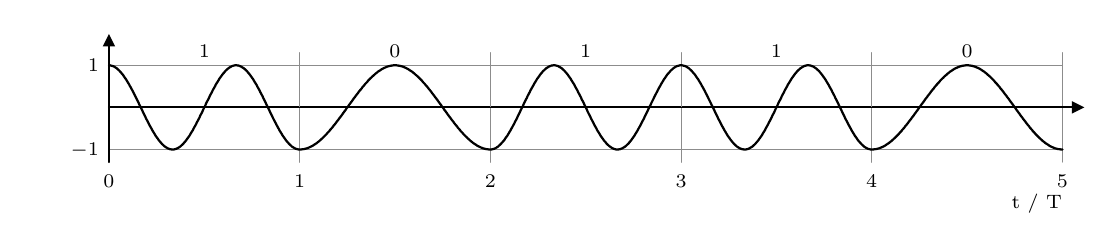
\begin{tikzpicture}[x=0.01985cm,y=-0.01985cm,line cap=round,line join=round]
\useasboundingbox (0,0) rectangle (680,120);
\path[draw=black!45,line width=0.35pt] (52,86) -- (52,16);
\path[draw=black!45,line width=0.35pt] (174,86) -- (174,16);
\path[draw=black!45,line width=0.35pt] (296,86) -- (296,16);
\path[draw=black!45,line width=0.35pt] (418,86) -- (418,16);
\path[draw=black!45,line width=0.35pt] (540,86) -- (540,16);
\path[draw=black!45,line width=0.35pt] (662,86) -- (662,16);
\path[draw=black!45,line width=0.35pt] (52,24.1) -- (662,24.1);
\path[draw=black!45,line width=0.35pt] (52,77.9) -- (662,77.9);
\path[draw=black,line width=0.7pt] (52,51) -- (670,51);
\path[fill=black,draw=none] (676,51) -- (668,47) -- (668,55) -- cycle;
\path[draw=black,line width=0.7pt] (52,86) -- (52,10);
\path[fill=black,draw=none] (52,4) -- (48,12) -- (56,12) -- cycle;
\node[anchor=base,inner sep=0pt,font=\scriptsize] at (52,102) {0};
\node[anchor=base,inner sep=0pt,font=\scriptsize] at (174,102) {1};
\node[anchor=base,inner sep=0pt,font=\scriptsize] at (296,102) {2};
\node[anchor=base,inner sep=0pt,font=\scriptsize] at (418,102) {3};
\node[anchor=base,inner sep=0pt,font=\scriptsize] at (540,102) {4};
\node[anchor=base,inner sep=0pt,font=\scriptsize] at (662,102) {5};
\node[anchor=base east,inner sep=0pt,font=\scriptsize] at (46,28.1) {1};
\node[anchor=base east,inner sep=0pt,font=\scriptsize] at (46,81.9) {$-$1};
\node[anchor=base east,inner sep=0pt,font=\scriptsize] at (662,116) {t / T};
\path[draw=black!45,line width=0.35pt,dash pattern=on 3pt off 2pt] (174,86) -- (174,16);
\path[draw=black!45,line width=0.35pt,dash pattern=on 3pt off 2pt] (296,86) -- (296,16);
\path[draw=black!45,line width=0.35pt,dash pattern=on 3pt off 2pt] (418,86) -- (418,16);
\path[draw=black!45,line width=0.35pt,dash pattern=on 3pt off 2pt] (540,86) -- (540,16);
\path[draw=black,line width=0.8pt] (52,24.1) -- (52.4,24.1) -- (52.8,24.1) -- (53.1,24.2) -- (53.5,24.3) -- (53.9,24.4) -- (54.3,24.5) -- (54.7,24.6) -- (55.1,24.8) -- (55.4,25) -- (55.8,25.2) -- (56.2,25.5) -- (56.6,25.7) -- (57,26) -- (57.3,26.3) -- (57.7,26.7) -- (58.1,27) -- (58.5,27.4) -- (58.9,27.8) -- (59.2,28.2) -- (59.6,28.6) -- (60,29.1) -- (60.4,29.5) -- (60.8,30) -- (61.2,30.5) -- (61.5,31.1) -- (61.9,31.6) -- (62.3,32.2) -- (62.7,32.7) -- (63.1,33.3) -- (63.4,33.9) -- (63.8,34.5) -- (64.2,35.2) -- (64.6,35.8) -- (65,36.5) -- (65.3,37.2) -- (65.7,37.8) -- (66.1,38.5) -- (66.5,39.3) -- (66.9,40) -- (67.3,40.7) -- (67.6,41.4) -- (68,42.2) -- (68.4,42.9) -- (68.8,43.7) -- (69.2,44.5) -- (69.5,45.2) -- (69.9,46) -- (70.3,46.8) -- (70.7,47.6) -- (71.1,48.4) -- (71.4,49.2) -- (71.8,49.9) -- (72.2,50.7) -- (72.6,51.5) -- (73,52.3) -- (73.4,53.1) -- (73.7,53.9) -- (74.1,54.7) -- (74.5,55.5) -- (74.9,56.3) -- (75.3,57) -- (75.6,57.8) -- (76,58.6) -- (76.4,59.3) -- (76.8,60.1) -- (77.2,60.8) -- (77.5,61.5) -- (77.9,62.3) -- (78.3,63) -- (78.7,63.7) -- (79.1,64.4) -- (79.5,65.1) -- (79.8,65.7) -- (80.2,66.4) -- (80.6,67) -- (81,67.7) -- (81.4,68.3) -- (81.7,68.9) -- (82.1,69.5) -- (82.5,70) -- (82.9,70.6) -- (83.3,71.1) -- (83.6,71.6) -- (84,72.1) -- (84.4,72.6) -- (84.8,73.1) -- (85.2,73.5) -- (85.6,74) -- (85.9,74.4) -- (86.3,74.7) -- (86.7,75.1) -- (87.1,75.5) -- (87.5,75.8) -- (87.8,76.1) -- (88.2,76.3) -- (88.6,76.6) -- (89,76.8) -- (89.4,77.1) -- (89.7,77.2) -- (90.1,77.4) -- (90.5,77.5) -- (90.9,77.7) -- (91.3,77.8) -- (91.7,77.8) -- (92,77.9) -- (92.4,77.9) -- (92.8,77.9) -- (93.2,77.9) -- (93.6,77.9) -- (93.9,77.8) -- (94.3,77.7) -- (94.7,77.6) -- (95.1,77.5) -- (95.5,77.3) -- (95.8,77.1) -- (96.2,76.9) -- (96.6,76.7) -- (97,76.4) -- (97.4,76.2) -- (97.8,75.9) -- (98.1,75.6) -- (98.5,75.2) -- (98.9,74.9) -- (99.3,74.5) -- (99.7,74.1) -- (100,73.7) -- (100.4,73.2) -- (100.8,72.8) -- (101.2,72.3) -- (101.6,71.8) -- (101.9,71.3) -- (102.3,70.8) -- (102.7,70.2) -- (103.1,69.7) -- (103.5,69.1) -- (103.9,68.5) -- (104.2,67.9) -- (104.6,67.2) -- (105,66.6) -- (105.4,66) -- (105.8,65.3) -- (106.1,64.6) -- (106.5,63.9) -- (106.9,63.2) -- (107.3,62.5) -- (107.7,61.8) -- (108,61.1) -- (108.4,60.3) -- (108.8,59.6) -- (109.2,58.8) -- (109.6,58.1) -- (110,57.3) -- (110.3,56.5) -- (110.7,55.7) -- (111.1,55) -- (111.5,54.2) -- (111.9,53.4) -- (112.2,52.6) -- (112.6,51.8) -- (113,51) -- (113.4,50.2) -- (113.8,49.4) -- (114.1,48.6) -- (114.5,47.8) -- (114.9,47) -- (115.3,46.3) -- (115.7,45.5) -- (116.1,44.7) -- (116.4,43.9) -- (116.8,43.2) -- (117.2,42.4) -- (117.6,41.7) -- (118,40.9) -- (118.3,40.2) -- (118.7,39.5) -- (119.1,38.8) -- (119.5,38.1) -- (119.9,37.4) -- (120.2,36.7) -- (120.6,36) -- (121,35.4) -- (121.4,34.8) -- (121.8,34.1) -- (122.2,33.5) -- (122.5,32.9) -- (122.9,32.3) -- (123.3,31.8) -- (123.7,31.2) -- (124.1,30.7) -- (124.4,30.2) -- (124.8,29.7) -- (125.2,29.2) -- (125.6,28.8) -- (126,28.3) -- (126.3,27.9) -- (126.7,27.5) -- (127.1,27.1) -- (127.5,26.8) -- (127.9,26.4) -- (128.3,26.1) -- (128.6,25.8) -- (129,25.6) -- (129.4,25.3) -- (129.8,25.1) -- (130.2,24.9) -- (130.5,24.7) -- (130.9,24.5) -- (131.3,24.4) -- (131.7,24.3) -- (132.1,24.2) -- (132.4,24.1) -- (132.8,24.1) -- (133.2,24.1) -- (133.6,24.1) -- (134,24.1) -- (134.4,24.2) -- (134.7,24.2) -- (135.1,24.3) -- (135.5,24.5) -- (135.9,24.6) -- (136.3,24.8) -- (136.6,24.9) -- (137,25.2) -- (137.4,25.4) -- (137.8,25.7) -- (138.2,25.9) -- (138.5,26.2) -- (138.9,26.5) -- (139.3,26.9) -- (139.7,27.3) -- (140.1,27.6) -- (140.5,28) -- (140.8,28.5) -- (141.2,28.9) -- (141.6,29.4) -- (142,29.9) -- (142.4,30.4) -- (142.7,30.9) -- (143.1,31.4) -- (143.5,32) -- (143.9,32.5) -- (144.3,33.1) -- (144.6,33.7) -- (145,34.3) -- (145.4,35) -- (145.8,35.6) -- (146.2,36.3) -- (146.6,36.9) -- (146.9,37.6) -- (147.3,38.3) -- (147.7,39) -- (148.1,39.7) -- (148.5,40.5) -- (148.8,41.2) -- (149.2,41.9) -- (149.6,42.7) -- (150,43.4) -- (150.4,44.2) -- (150.7,45) -- (151.1,45.7) -- (151.5,46.5) -- (151.9,47.3) -- (152.3,48.1) -- (152.6,48.9) -- (153,49.7) -- (153.4,50.5) -- (153.8,51.3) -- (154.2,52.1) -- (154.6,52.8) -- (154.9,53.6) -- (155.3,54.4) -- (155.7,55.2) -- (156.1,56) -- (156.5,56.8) -- (156.8,57.5) -- (157.2,58.3) -- (157.6,59.1) -- (158,59.8) -- (158.4,60.6) -- (158.8,61.3) -- (159.1,62) -- (159.5,62.7) -- (159.9,63.5) -- (160.3,64.2) -- (160.7,64.8) -- (161,65.5) -- (161.4,66.2) -- (161.8,66.8) -- (162.2,67.5) -- (162.6,68.1) -- (162.9,68.7) -- (163.3,69.3) -- (163.7,69.8) -- (164.1,70.4) -- (164.5,70.9) -- (164.9,71.5) -- (165.2,72) -- (165.6,72.5) -- (166,72.9) -- (166.4,73.4) -- (166.8,73.8) -- (167.1,74.2) -- (167.5,74.6) -- (167.9,75) -- (168.3,75.3) -- (168.7,75.7) -- (169,76) -- (169.4,76.3) -- (169.8,76.5) -- (170.2,76.8) -- (170.6,77) -- (171,77.2) -- (171.3,77.4) -- (171.7,77.5) -- (172.1,77.6) -- (172.5,77.7) -- (172.9,77.8) -- (173.2,77.9) -- (173.6,77.9) -- (174,77.9) -- (174.4,77.9) -- (174.8,77.9) -- (175.1,77.9) -- (175.5,77.8) -- (175.9,77.8) -- (176.3,77.7) -- (176.7,77.7) -- (177.1,77.6) -- (177.4,77.5) -- (177.8,77.4) -- (178.2,77.3) -- (178.6,77.2) -- (179,77.1) -- (179.3,76.9) -- (179.7,76.8) -- (180.1,76.6) -- (180.5,76.4) -- (180.9,76.3) -- (181.2,76.1) -- (181.6,75.9) -- (182,75.7) -- (182.4,75.5) -- (182.8,75.2) -- (183.2,75) -- (183.5,74.7) -- (183.9,74.5) -- (184.3,74.2) -- (184.7,74) -- (185.1,73.7) -- (185.4,73.4) -- (185.8,73.1) -- (186.2,72.8) -- (186.6,72.5) -- (187,72.1) -- (187.3,71.8) -- (187.7,71.5) -- (188.1,71.1) -- (188.5,70.8) -- (188.9,70.4) -- (189.3,70) -- (189.6,69.7) -- (190,69.3) -- (190.4,68.9) -- (190.8,68.5) -- (191.2,68.1) -- (191.5,67.7) -- (191.9,67.2) -- (192.3,66.8) -- (192.7,66.4) -- (193.1,66) -- (193.4,65.5) -- (193.8,65.1) -- (194.2,64.6) -- (194.6,64.2) -- (195,63.7) -- (195.4,63.2) -- (195.7,62.7) -- (196.1,62.3) -- (196.5,61.8) -- (196.9,61.3) -- (197.3,60.8) -- (197.6,60.3) -- (198,59.8) -- (198.4,59.3) -- (198.8,58.8) -- (199.2,58.3) -- (199.5,57.8) -- (199.9,57.3) -- (200.3,56.8) -- (200.7,56.3) -- (201.1,55.7) -- (201.5,55.2) -- (201.8,54.7) -- (202.2,54.2) -- (202.6,53.6) -- (203,53.1) -- (203.4,52.6) -- (203.7,52.1) -- (204.1,51.5) -- (204.5,51) -- (204.9,50.5) -- (205.3,49.9) -- (205.6,49.4) -- (206,48.9) -- (206.4,48.4) -- (206.8,47.8) -- (207.2,47.3) -- (207.6,46.8) -- (207.9,46.3) -- (208.3,45.7) -- (208.7,45.2) -- (209.1,44.7) -- (209.5,44.2) -- (209.8,43.7) -- (210.2,43.2) -- (210.6,42.7) -- (211,42.2) -- (211.4,41.7) -- (211.7,41.2) -- (212.1,40.7) -- (212.5,40.2) -- (212.9,39.7) -- (213.3,39.3) -- (213.7,38.8) -- (214,38.3) -- (214.4,37.8) -- (214.8,37.4) -- (215.2,36.9) -- (215.6,36.5) -- (215.9,36) -- (216.3,35.6) -- (216.7,35.2) -- (217.1,34.8) -- (217.5,34.3) -- (217.8,33.9) -- (218.2,33.5) -- (218.6,33.1) -- (219,32.7) -- (219.4,32.3) -- (219.8,32) -- (220.1,31.6) -- (220.5,31.2) -- (220.9,30.9) -- (221.3,30.5) -- (221.7,30.2) -- (222,29.9) -- (222.4,29.5) -- (222.8,29.2) -- (223.2,28.9) -- (223.6,28.6) -- (223.9,28.3) -- (224.3,28) -- (224.7,27.8) -- (225.1,27.5) -- (225.5,27.3) -- (225.9,27) -- (226.2,26.8) -- (226.6,26.5) -- (227,26.3) -- (227.4,26.1) -- (227.8,25.9) -- (228.1,25.7) -- (228.5,25.6) -- (228.9,25.4) -- (229.3,25.2) -- (229.7,25.1) -- (230,24.9) -- (230.4,24.8) -- (230.8,24.7) -- (231.2,24.6) -- (231.6,24.5) -- (232,24.4) -- (232.3,24.3) -- (232.7,24.3) -- (233.1,24.2) -- (233.5,24.2) -- (233.9,24.1) -- (234.2,24.1) -- (234.6,24.1) -- (235,24.1) -- (235.4,24.1) -- (235.8,24.1) -- (236.1,24.1) -- (236.5,24.2) -- (236.9,24.2) -- (237.3,24.3) -- (237.7,24.3) -- (238.1,24.4) -- (238.4,24.5) -- (238.8,24.6) -- (239.2,24.7) -- (239.6,24.8) -- (240,24.9) -- (240.3,25.1) -- (240.7,25.2) -- (241.1,25.4) -- (241.5,25.6) -- (241.9,25.7) -- (242.2,25.9) -- (242.6,26.1) -- (243,26.3) -- (243.4,26.5) -- (243.8,26.8) -- (244.2,27) -- (244.5,27.3) -- (244.9,27.5) -- (245.3,27.8) -- (245.7,28) -- (246.1,28.3) -- (246.4,28.6) -- (246.8,28.9) -- (247.2,29.2) -- (247.6,29.5) -- (248,29.9) -- (248.3,30.2) -- (248.7,30.5) -- (249.1,30.9) -- (249.5,31.2) -- (249.9,31.6) -- (250.3,32) -- (250.6,32.3) -- (251,32.7) -- (251.4,33.1) -- (251.8,33.5) -- (252.2,33.9) -- (252.5,34.3) -- (252.9,34.8) -- (253.3,35.2) -- (253.7,35.6) -- (254.1,36) -- (254.4,36.5) -- (254.8,36.9) -- (255.2,37.4) -- (255.6,37.8) -- (256,38.3) -- (256.4,38.8) -- (256.7,39.3) -- (257.1,39.7) -- (257.5,40.2) -- (257.9,40.7) -- (258.3,41.2) -- (258.6,41.7) -- (259,42.2) -- (259.4,42.7) -- (259.8,43.2) -- (260.2,43.7) -- (260.5,44.2) -- (260.9,44.7) -- (261.3,45.2) -- (261.7,45.7) -- (262.1,46.3) -- (262.5,46.8) -- (262.8,47.3) -- (263.2,47.8) -- (263.6,48.4) -- (264,48.9) -- (264.4,49.4) -- (264.7,49.9) -- (265.1,50.5) -- (265.5,51) -- (265.9,51.5) -- (266.3,52.1) -- (266.6,52.6) -- (267,53.1) -- (267.4,53.6) -- (267.8,54.2) -- (268.2,54.7) -- (268.5,55.2) -- (268.9,55.7) -- (269.3,56.3) -- (269.7,56.8) -- (270.1,57.3) -- (270.5,57.8) -- (270.8,58.3) -- (271.2,58.8) -- (271.6,59.3) -- (272,59.8) -- (272.4,60.3) -- (272.7,60.8) -- (273.1,61.3) -- (273.5,61.8) -- (273.9,62.3) -- (274.3,62.7) -- (274.7,63.2) -- (275,63.7) -- (275.4,64.2) -- (275.8,64.6) -- (276.2,65.1) -- (276.6,65.5) -- (276.9,66) -- (277.3,66.4) -- (277.7,66.8) -- (278.1,67.2) -- (278.5,67.7) -- (278.8,68.1) -- (279.2,68.5) -- (279.6,68.9) -- (280,69.3) -- (280.4,69.7) -- (280.8,70) -- (281.1,70.4) -- (281.5,70.8) -- (281.9,71.1) -- (282.3,71.5) -- (282.7,71.8) -- (283,72.1) -- (283.4,72.5) -- (283.8,72.8) -- (284.2,73.1) -- (284.6,73.4) -- (284.9,73.7) -- (285.3,74) -- (285.7,74.2) -- (286.1,74.5) -- (286.5,74.7) -- (286.9,75) -- (287.2,75.2) -- (287.6,75.5) -- (288,75.7) -- (288.4,75.9) -- (288.8,76.1) -- (289.1,76.3) -- (289.5,76.4) -- (289.9,76.6) -- (290.3,76.8) -- (290.7,76.9) -- (291,77.1) -- (291.4,77.2) -- (291.8,77.3) -- (292.2,77.4) -- (292.6,77.5) -- (293,77.6) -- (293.3,77.7) -- (293.7,77.7) -- (294.1,77.8) -- (294.5,77.8) -- (294.9,77.9) -- (295.2,77.9) -- (295.6,77.9) -- (296,77.9) -- (296.4,77.9) -- (296.8,77.9) -- (297.1,77.8) -- (297.5,77.7) -- (297.9,77.6) -- (298.3,77.5) -- (298.7,77.4) -- (299,77.2) -- (299.4,77) -- (299.8,76.8) -- (300.2,76.5) -- (300.6,76.3) -- (301,76) -- (301.3,75.7) -- (301.7,75.3) -- (302.1,75) -- (302.5,74.6) -- (302.9,74.2) -- (303.2,73.8) -- (303.6,73.4) -- (304,72.9) -- (304.4,72.5) -- (304.8,72) -- (305.2,71.5) -- (305.5,70.9) -- (305.9,70.4) -- (306.3,69.8) -- (306.7,69.3) -- (307.1,68.7) -- (307.4,68.1) -- (307.8,67.5) -- (308.2,66.8) -- (308.6,66.2) -- (309,65.5) -- (309.3,64.8) -- (309.7,64.2) -- (310.1,63.5) -- (310.5,62.7) -- (310.9,62) -- (311.3,61.3) -- (311.6,60.6) -- (312,59.8) -- (312.4,59.1) -- (312.8,58.3) -- (313.2,57.5) -- (313.5,56.8) -- (313.9,56) -- (314.3,55.2) -- (314.7,54.4) -- (315.1,53.6) -- (315.4,52.8) -- (315.8,52.1) -- (316.2,51.3) -- (316.6,50.5) -- (317,49.7) -- (317.3,48.9) -- (317.7,48.1) -- (318.1,47.3) -- (318.5,46.5) -- (318.9,45.7) -- (319.3,45) -- (319.6,44.2) -- (320,43.4) -- (320.4,42.7) -- (320.8,41.9) -- (321.2,41.2) -- (321.5,40.5) -- (321.9,39.7) -- (322.3,39) -- (322.7,38.3) -- (323.1,37.6) -- (323.5,36.9) -- (323.8,36.3) -- (324.2,35.6) -- (324.6,35) -- (325,34.3) -- (325.4,33.7) -- (325.7,33.1) -- (326.1,32.5) -- (326.5,32) -- (326.9,31.4) -- (327.3,30.9) -- (327.6,30.4) -- (328,29.9) -- (328.4,29.4) -- (328.8,28.9) -- (329.2,28.5) -- (329.5,28) -- (329.9,27.6) -- (330.3,27.3) -- (330.7,26.9) -- (331.1,26.5) -- (331.5,26.2) -- (331.8,25.9) -- (332.2,25.7) -- (332.6,25.4) -- (333,25.2) -- (333.4,24.9) -- (333.7,24.8) -- (334.1,24.6) -- (334.5,24.5) -- (334.9,24.3) -- (335.3,24.2) -- (335.7,24.2) -- (336,24.1) -- (336.4,24.1) -- (336.8,24.1) -- (337.2,24.1) -- (337.6,24.1) -- (337.9,24.2) -- (338.3,24.3) -- (338.7,24.4) -- (339.1,24.5) -- (339.5,24.7) -- (339.8,24.9) -- (340.2,25.1) -- (340.6,25.3) -- (341,25.6) -- (341.4,25.8) -- (341.8,26.1) -- (342.1,26.4) -- (342.5,26.8) -- (342.9,27.1) -- (343.3,27.5) -- (343.7,27.9) -- (344,28.3) -- (344.4,28.8) -- (344.8,29.2) -- (345.2,29.7) -- (345.6,30.2) -- (345.9,30.7) -- (346.3,31.2) -- (346.7,31.8) -- (347.1,32.3) -- (347.5,32.9) -- (347.8,33.5) -- (348.2,34.1) -- (348.6,34.8) -- (349,35.4) -- (349.4,36) -- (349.8,36.7) -- (350.1,37.4) -- (350.5,38.1) -- (350.9,38.8) -- (351.3,39.5) -- (351.7,40.2) -- (352,40.9) -- (352.4,41.7) -- (352.8,42.4) -- (353.2,43.2) -- (353.6,43.9) -- (354,44.7) -- (354.3,45.5) -- (354.7,46.3) -- (355.1,47) -- (355.5,47.8) -- (355.9,48.6) -- (356.2,49.4) -- (356.6,50.2) -- (357,51) -- (357.4,51.8) -- (357.8,52.6) -- (358.1,53.4) -- (358.5,54.2) -- (358.9,55) -- (359.3,55.7) -- (359.7,56.5) -- (360.1,57.3) -- (360.4,58.1) -- (360.8,58.8) -- (361.2,59.6) -- (361.6,60.3) -- (362,61.1) -- (362.3,61.8) -- (362.7,62.5) -- (363.1,63.2) -- (363.5,63.9) -- (363.9,64.6) -- (364.2,65.3) -- (364.6,66) -- (365,66.6) -- (365.4,67.2) -- (365.8,67.9) -- (366.2,68.5) -- (366.5,69.1) -- (366.9,69.7) -- (367.3,70.2) -- (367.7,70.8) -- (368.1,71.3) -- (368.4,71.8) -- (368.8,72.3) -- (369.2,72.8) -- (369.6,73.2) -- (370,73.7) -- (370.3,74.1) -- (370.7,74.5) -- (371.1,74.9) -- (371.5,75.2) -- (371.9,75.6) -- (372.3,75.9) -- (372.6,76.2) -- (373,76.4) -- (373.4,76.7) -- (373.8,76.9) -- (374.2,77.1) -- (374.5,77.3) -- (374.9,77.5) -- (375.3,77.6) -- (375.7,77.7) -- (376.1,77.8) -- (376.4,77.9) -- (376.8,77.9) -- (377.2,77.9) -- (377.6,77.9) -- (378,77.9) -- (378.3,77.8) -- (378.7,77.8) -- (379.1,77.7) -- (379.5,77.5) -- (379.9,77.4) -- (380.3,77.2) -- (380.6,77.1) -- (381,76.8) -- (381.4,76.6) -- (381.8,76.3) -- (382.2,76.1) -- (382.5,75.8) -- (382.9,75.5) -- (383.3,75.1) -- (383.7,74.7) -- (384.1,74.4) -- (384.5,74) -- (384.8,73.5) -- (385.2,73.1) -- (385.6,72.6) -- (386,72.1) -- (386.4,71.6) -- (386.7,71.1) -- (387.1,70.6) -- (387.5,70) -- (387.9,69.5) -- (388.3,68.9) -- (388.6,68.3) -- (389,67.7) -- (389.4,67) -- (389.8,66.4) -- (390.2,65.7) -- (390.5,65.1) -- (390.9,64.4) -- (391.3,63.7) -- (391.7,63) -- (392.1,62.3) -- (392.5,61.5) -- (392.8,60.8) -- (393.2,60.1) -- (393.6,59.3) -- (394,58.6) -- (394.4,57.8) -- (394.7,57) -- (395.1,56.3) -- (395.5,55.5) -- (395.9,54.7) -- (396.3,53.9) -- (396.7,53.1) -- (397,52.3) -- (397.4,51.5) -- (397.8,50.7) -- (398.2,49.9) -- (398.6,49.2) -- (398.9,48.4) -- (399.3,47.6) -- (399.7,46.8) -- (400.1,46) -- (400.5,45.2) -- (400.8,44.5) -- (401.2,43.7) -- (401.6,42.9) -- (402,42.2) -- (402.4,41.4) -- (402.8,40.7) -- (403.1,40) -- (403.5,39.3) -- (403.9,38.5) -- (404.3,37.8) -- (404.7,37.2) -- (405,36.5) -- (405.4,35.8) -- (405.8,35.2) -- (406.2,34.5) -- (406.6,33.9) -- (406.9,33.3) -- (407.3,32.7) -- (407.7,32.2) -- (408.1,31.6) -- (408.5,31.1) -- (408.8,30.5) -- (409.2,30) -- (409.6,29.5) -- (410,29.1) -- (410.4,28.6) -- (410.8,28.2) -- (411.1,27.8) -- (411.5,27.4) -- (411.9,27) -- (412.3,26.7) -- (412.7,26.3) -- (413,26) -- (413.4,25.7) -- (413.8,25.5) -- (414.2,25.2) -- (414.6,25) -- (415,24.8) -- (415.3,24.6) -- (415.7,24.5) -- (416.1,24.4) -- (416.5,24.3) -- (416.9,24.2) -- (417.2,24.1) -- (417.6,24.1) -- (418,24.1) -- (418.4,24.1) -- (418.8,24.1) -- (419.1,24.2) -- (419.5,24.3) -- (419.9,24.4) -- (420.3,24.5) -- (420.7,24.6) -- (421.1,24.8) -- (421.4,25) -- (421.8,25.2) -- (422.2,25.5) -- (422.6,25.7) -- (423,26) -- (423.3,26.3) -- (423.7,26.7) -- (424.1,27) -- (424.5,27.4) -- (424.9,27.8) -- (425.2,28.2) -- (425.6,28.6) -- (426,29.1) -- (426.4,29.5) -- (426.8,30) -- (427.2,30.5) -- (427.5,31.1) -- (427.9,31.6) -- (428.3,32.2) -- (428.7,32.7) -- (429.1,33.3) -- (429.4,33.9) -- (429.8,34.5) -- (430.2,35.2) -- (430.6,35.8) -- (431,36.5) -- (431.3,37.2) -- (431.7,37.8) -- (432.1,38.5) -- (432.5,39.3) -- (432.9,40) -- (433.3,40.7) -- (433.6,41.4) -- (434,42.2) -- (434.4,42.9) -- (434.8,43.7) -- (435.2,44.5) -- (435.5,45.2) -- (435.9,46) -- (436.3,46.8) -- (436.7,47.6) -- (437.1,48.4) -- (437.4,49.2) -- (437.8,49.9) -- (438.2,50.7) -- (438.6,51.5) -- (439,52.3) -- (439.4,53.1) -- (439.7,53.9) -- (440.1,54.7) -- (440.5,55.5) -- (440.9,56.3) -- (441.3,57) -- (441.6,57.8) -- (442,58.6) -- (442.4,59.3) -- (442.8,60.1) -- (443.2,60.8) -- (443.5,61.5) -- (443.9,62.3) -- (444.3,63) -- (444.7,63.7) -- (445.1,64.4) -- (445.5,65.1) -- (445.8,65.7) -- (446.2,66.4) -- (446.6,67) -- (447,67.7) -- (447.4,68.3) -- (447.7,68.9) -- (448.1,69.5) -- (448.5,70) -- (448.9,70.6) -- (449.3,71.1) -- (449.6,71.6) -- (450,72.1) -- (450.4,72.6) -- (450.8,73.1) -- (451.2,73.5) -- (451.6,74) -- (451.9,74.4) -- (452.3,74.7) -- (452.7,75.1) -- (453.1,75.5) -- (453.5,75.8) -- (453.8,76.1) -- (454.2,76.3) -- (454.6,76.6) -- (455,76.8) -- (455.4,77.1) -- (455.7,77.2) -- (456.1,77.4) -- (456.5,77.5) -- (456.9,77.7) -- (457.3,77.8) -- (457.7,77.8) -- (458,77.9) -- (458.4,77.9) -- (458.8,77.9) -- (459.2,77.9) -- (459.6,77.9) -- (459.9,77.8) -- (460.3,77.7) -- (460.7,77.6) -- (461.1,77.5) -- (461.5,77.3) -- (461.8,77.1) -- (462.2,76.9) -- (462.6,76.7) -- (463,76.4) -- (463.4,76.2) -- (463.8,75.9) -- (464.1,75.6) -- (464.5,75.2) -- (464.9,74.9) -- (465.3,74.5) -- (465.7,74.1) -- (466,73.7) -- (466.4,73.2) -- (466.8,72.8) -- (467.2,72.3) -- (467.6,71.8) -- (467.9,71.3) -- (468.3,70.8) -- (468.7,70.2) -- (469.1,69.7) -- (469.5,69.1) -- (469.9,68.5) -- (470.2,67.9) -- (470.6,67.2) -- (471,66.6) -- (471.4,66) -- (471.8,65.3) -- (472.1,64.6) -- (472.5,63.9) -- (472.9,63.2) -- (473.3,62.5) -- (473.7,61.8) -- (474,61.1) -- (474.4,60.3) -- (474.8,59.6) -- (475.2,58.8) -- (475.6,58.1) -- (476,57.3) -- (476.3,56.5) -- (476.7,55.7) -- (477.1,55) -- (477.5,54.2) -- (477.9,53.4) -- (478.2,52.6) -- (478.6,51.8) -- (479,51) -- (479.4,50.2) -- (479.8,49.4) -- (480.1,48.6) -- (480.5,47.8) -- (480.9,47) -- (481.3,46.3) -- (481.7,45.5) -- (482.1,44.7) -- (482.4,43.9) -- (482.8,43.2) -- (483.2,42.4) -- (483.6,41.7) -- (484,40.9) -- (484.3,40.2) -- (484.7,39.5) -- (485.1,38.8) -- (485.5,38.1) -- (485.9,37.4) -- (486.2,36.7) -- (486.6,36) -- (487,35.4) -- (487.4,34.8) -- (487.8,34.1) -- (488.2,33.5) -- (488.5,32.9) -- (488.9,32.3) -- (489.3,31.8) -- (489.7,31.2) -- (490.1,30.7) -- (490.4,30.2) -- (490.8,29.7) -- (491.2,29.2) -- (491.6,28.8) -- (492,28.3) -- (492.3,27.9) -- (492.7,27.5) -- (493.1,27.1) -- (493.5,26.8) -- (493.9,26.4) -- (494.3,26.1) -- (494.6,25.8) -- (495,25.6) -- (495.4,25.3) -- (495.8,25.1) -- (496.2,24.9) -- (496.5,24.7) -- (496.9,24.5) -- (497.3,24.4) -- (497.7,24.3) -- (498.1,24.2) -- (498.4,24.1) -- (498.8,24.1) -- (499.2,24.1) -- (499.6,24.1) -- (500,24.1) -- (500.4,24.2) -- (500.7,24.2) -- (501.1,24.3) -- (501.5,24.5) -- (501.9,24.6) -- (502.3,24.8) -- (502.6,24.9) -- (503,25.2) -- (503.4,25.4) -- (503.8,25.7) -- (504.2,25.9) -- (504.5,26.2) -- (504.9,26.5) -- (505.3,26.9) -- (505.7,27.3) -- (506.1,27.6) -- (506.5,28) -- (506.8,28.5) -- (507.2,28.9) -- (507.6,29.4) -- (508,29.9) -- (508.4,30.4) -- (508.7,30.9) -- (509.1,31.4) -- (509.5,32) -- (509.9,32.5) -- (510.3,33.1) -- (510.6,33.7) -- (511,34.3) -- (511.4,35) -- (511.8,35.6) -- (512.2,36.3) -- (512.6,36.9) -- (512.9,37.6) -- (513.3,38.3) -- (513.7,39) -- (514.1,39.7) -- (514.5,40.5) -- (514.8,41.2) -- (515.2,41.9) -- (515.6,42.7) -- (516,43.4) -- (516.4,44.2) -- (516.7,45) -- (517.1,45.7) -- (517.5,46.5) -- (517.9,47.3) -- (518.3,48.1) -- (518.7,48.9) -- (519,49.7) -- (519.4,50.5) -- (519.8,51.3) -- (520.2,52.1) -- (520.6,52.8) -- (520.9,53.6) -- (521.3,54.4) -- (521.7,55.2) -- (522.1,56) -- (522.5,56.8) -- (522.8,57.5) -- (523.2,58.3) -- (523.6,59.1) -- (524,59.8) -- (524.4,60.6) -- (524.8,61.3) -- (525.1,62) -- (525.5,62.7) -- (525.9,63.5) -- (526.3,64.2) -- (526.7,64.8) -- (527,65.5) -- (527.4,66.2) -- (527.8,66.8) -- (528.2,67.5) -- (528.6,68.1) -- (528.9,68.7) -- (529.3,69.3) -- (529.7,69.8) -- (530.1,70.4) -- (530.5,70.9) -- (530.8,71.5) -- (531.2,72) -- (531.6,72.5) -- (532,72.9) -- (532.4,73.4) -- (532.8,73.8) -- (533.1,74.2) -- (533.5,74.6) -- (533.9,75) -- (534.3,75.3) -- (534.7,75.7) -- (535,76) -- (535.4,76.3) -- (535.8,76.5) -- (536.2,76.8) -- (536.6,77) -- (537,77.2) -- (537.3,77.4) -- (537.7,77.5) -- (538.1,77.6) -- (538.5,77.7) -- (538.9,77.8) -- (539.2,77.9) -- (539.6,77.9) -- (540,77.9) -- (540.4,77.9) -- (540.8,77.9) -- (541.1,77.9) -- (541.5,77.8) -- (541.9,77.8) -- (542.3,77.7) -- (542.7,77.7) -- (543.1,77.6) -- (543.4,77.5) -- (543.8,77.4) -- (544.2,77.3) -- (544.6,77.2) -- (545,77.1) -- (545.3,76.9) -- (545.7,76.8) -- (546.1,76.6) -- (546.5,76.4) -- (546.9,76.3) -- (547.2,76.1) -- (547.6,75.9) -- (548,75.7) -- (548.4,75.5) -- (548.8,75.2) -- (549.2,75) -- (549.5,74.7) -- (549.9,74.5) -- (550.3,74.2) -- (550.7,74) -- (551.1,73.7) -- (551.4,73.4) -- (551.8,73.1) -- (552.2,72.8) -- (552.6,72.5) -- (553,72.1) -- (553.3,71.8) -- (553.7,71.5) -- (554.1,71.1) -- (554.5,70.8) -- (554.9,70.4) -- (555.3,70) -- (555.6,69.7) -- (556,69.3) -- (556.4,68.9) -- (556.8,68.5) -- (557.2,68.1) -- (557.5,67.7) -- (557.9,67.2) -- (558.3,66.8) -- (558.7,66.4) -- (559.1,66) -- (559.4,65.5) -- (559.8,65.1) -- (560.2,64.6) -- (560.6,64.2) -- (561,63.7) -- (561.3,63.2) -- (561.7,62.7) -- (562.1,62.3) -- (562.5,61.8) -- (562.9,61.3) -- (563.3,60.8) -- (563.6,60.3) -- (564,59.8) -- (564.4,59.3) -- (564.8,58.8) -- (565.2,58.3) -- (565.5,57.8) -- (565.9,57.3) -- (566.3,56.8) -- (566.7,56.3) -- (567.1,55.7) -- (567.4,55.2) -- (567.8,54.7) -- (568.2,54.2) -- (568.6,53.6) -- (569,53.1) -- (569.4,52.6) -- (569.7,52.1) -- (570.1,51.5) -- (570.5,51) -- (570.9,50.5) -- (571.3,49.9) -- (571.6,49.4) -- (572,48.9) -- (572.4,48.4) -- (572.8,47.8) -- (573.2,47.3) -- (573.6,46.8) -- (573.9,46.3) -- (574.3,45.7) -- (574.7,45.2) -- (575.1,44.7) -- (575.5,44.2) -- (575.8,43.7) -- (576.2,43.2) -- (576.6,42.7) -- (577,42.2) -- (577.4,41.7) -- (577.7,41.2) -- (578.1,40.7) -- (578.5,40.2) -- (578.9,39.7) -- (579.3,39.3) -- (579.7,38.8) -- (580,38.3) -- (580.4,37.8) -- (580.8,37.4) -- (581.2,36.9) -- (581.6,36.5) -- (581.9,36) -- (582.3,35.6) -- (582.7,35.2) -- (583.1,34.8) -- (583.5,34.3) -- (583.8,33.9) -- (584.2,33.5) -- (584.6,33.1) -- (585,32.7) -- (585.4,32.3) -- (585.8,32) -- (586.1,31.6) -- (586.5,31.2) -- (586.9,30.9) -- (587.3,30.5) -- (587.7,30.2) -- (588,29.9) -- (588.4,29.5) -- (588.8,29.2) -- (589.2,28.9) -- (589.6,28.6) -- (589.9,28.3) -- (590.3,28) -- (590.7,27.8) -- (591.1,27.5) -- (591.5,27.3) -- (591.9,27) -- (592.2,26.8) -- (592.6,26.5) -- (593,26.3) -- (593.4,26.1) -- (593.8,25.9) -- (594.1,25.7) -- (594.5,25.6) -- (594.9,25.4) -- (595.3,25.2) -- (595.7,25.1) -- (596,24.9) -- (596.4,24.8) -- (596.8,24.7) -- (597.2,24.6) -- (597.6,24.5) -- (597.9,24.4) -- (598.3,24.3) -- (598.7,24.3) -- (599.1,24.2) -- (599.5,24.2) -- (599.9,24.1) -- (600.2,24.1) -- (600.6,24.1) -- (601,24.1) -- (601.4,24.1) -- (601.8,24.1) -- (602.1,24.1) -- (602.5,24.2) -- (602.9,24.2) -- (603.3,24.3) -- (603.7,24.3) -- (604.1,24.4) -- (604.4,24.5) -- (604.8,24.6) -- (605.2,24.7) -- (605.6,24.8) -- (606,24.9) -- (606.3,25.1) -- (606.7,25.2) -- (607.1,25.4) -- (607.5,25.6) -- (607.9,25.7) -- (608.2,25.9) -- (608.6,26.1) -- (609,26.3) -- (609.4,26.5) -- (609.8,26.8) -- (610.2,27) -- (610.5,27.3) -- (610.9,27.5) -- (611.3,27.8) -- (611.7,28) -- (612.1,28.3) -- (612.4,28.6) -- (612.8,28.9) -- (613.2,29.2) -- (613.6,29.5) -- (614,29.9) -- (614.3,30.2) -- (614.7,30.5) -- (615.1,30.9) -- (615.5,31.2) -- (615.9,31.6) -- (616.3,32) -- (616.6,32.3) -- (617,32.7) -- (617.4,33.1) -- (617.8,33.5) -- (618.2,33.9) -- (618.5,34.3) -- (618.9,34.8) -- (619.3,35.2) -- (619.7,35.6) -- (620.1,36) -- (620.4,36.5) -- (620.8,36.9) -- (621.2,37.4) -- (621.6,37.8) -- (622,38.3) -- (622.3,38.8) -- (622.7,39.3) -- (623.1,39.7) -- (623.5,40.2) -- (623.9,40.7) -- (624.3,41.2) -- (624.6,41.7) -- (625,42.2) -- (625.4,42.7) -- (625.8,43.2) -- (626.2,43.7) -- (626.5,44.2) -- (626.9,44.7) -- (627.3,45.2) -- (627.7,45.7) -- (628.1,46.3) -- (628.4,46.8) -- (628.8,47.3) -- (629.2,47.8) -- (629.6,48.4) -- (630,48.9) -- (630.4,49.4) -- (630.7,49.9) -- (631.1,50.5) -- (631.5,51) -- (631.9,51.5) -- (632.3,52.1) -- (632.6,52.6) -- (633,53.1) -- (633.4,53.6) -- (633.8,54.2) -- (634.2,54.7) -- (634.6,55.2) -- (634.9,55.7) -- (635.3,56.3) -- (635.7,56.8) -- (636.1,57.3) -- (636.5,57.8) -- (636.8,58.3) -- (637.2,58.8) -- (637.6,59.3) -- (638,59.8) -- (638.4,60.3) -- (638.7,60.8) -- (639.1,61.3) -- (639.5,61.8) -- (639.9,62.3) -- (640.3,62.7) -- (640.7,63.2) -- (641,63.7) -- (641.4,64.2) -- (641.8,64.6) -- (642.2,65.1) -- (642.6,65.5) -- (642.9,66) -- (643.3,66.4) -- (643.7,66.8) -- (644.1,67.2) -- (644.5,67.7) -- (644.8,68.1) -- (645.2,68.5) -- (645.6,68.9) -- (646,69.3) -- (646.4,69.7) -- (646.8,70) -- (647.1,70.4) -- (647.5,70.8) -- (647.9,71.1) -- (648.3,71.5) -- (648.7,71.8) -- (649,72.1) -- (649.4,72.5) -- (649.8,72.8) -- (650.2,73.1) -- (650.6,73.4) -- (650.9,73.7) -- (651.3,74) -- (651.7,74.2) -- (652.1,74.5) -- (652.5,74.7) -- (652.9,75) -- (653.2,75.2) -- (653.6,75.5) -- (654,75.7) -- (654.4,75.9) -- (654.8,76.1) -- (655.1,76.3) -- (655.5,76.4) -- (655.9,76.6) -- (656.3,76.8) -- (656.7,76.9) -- (657,77.1) -- (657.4,77.2) -- (657.8,77.3) -- (658.2,77.4) -- (658.6,77.5) -- (658.9,77.6) -- (659.3,77.7) -- (659.7,77.7) -- (660.1,77.8) -- (660.5,77.8) -- (660.9,77.9) -- (661.2,77.9) -- (661.6,77.9) -- (662,77.9);
\node[anchor=base,inner sep=0pt,font=\scriptsize] at (113,18.8) {1};
\node[anchor=base,inner sep=0pt,font=\scriptsize] at (235,18.8) {0};
\node[anchor=base,inner sep=0pt,font=\scriptsize] at (357,18.8) {1};
\node[anchor=base,inner sep=0pt,font=\scriptsize] at (479,18.8) {1};
\node[anchor=base,inner sep=0pt,font=\scriptsize] at (601,18.8) {0};
\end{tikzpicture}\end{center}
\begin{itemize}
\item OOK: 1-nél egy vivőperiódus, 0-nál semmi. BPSK: 0-nál ellentétes fázis. FSK: 0-nál 1, 1-nél 1,5 periódus bitenként, folytonos fázissal.
\end{itemize}
\end{rajz}
\begin{eredmeny}

\begin{center}\adjustbox{max width=\linewidth}{$\displaystyle f_D=\frac1{4T}\ \text{(MSK)}$}\end{center}
\end{eredmeny}


% ------------------------------------------------------------------
\section{\texorpdfstring{7.5. feladat: 16-PSK $\surd$2 sugárral és BPSK csúcstényezője}{7.5. feladat: 16-PSK √2 sugárral és BPSK csúcstényezője}}\label{ai7_05}
\setcounter{lepes}{0}
\begin{feladat}{7.5. feladat}
a) 16-PSK, a konstelláció sugara $\sqrt2$: átlagteljesítmény? Hogyan változik a szükséges SNR 11,25\textdegree{}-os fázishiba esetén? b) Mekkora egy 1 kHz-es, 2 V-os BPSK jel csúcstényezője?

{\footnotesize\sffamily Forrás: ALL-IN 21., 127. oldal $\cdot$ ai2016\_01\_05\_6, aiD\_7\_10 (és 5-ösöm 2. oldal). Címkék: beugró}
\end{feladat}
\begin{keresunk}
\begin{itemize}
\item a) $P$ (átlagteljesítmény) és az SNR változása
\item b) $C$ (csúcstényező)
\end{itemize}
\end{keresunk}
\begin{jeloles}
\begin{jeltabla}
$\ca{U}$ & a jel amplitúdója & $2$\,V\\
$\cb{f_v}$ & vivőfrekvencia & $1$\,kHz\\
$P$ & átlagteljesítmény & \emph{keresett}\\
$C$ & csúcstényező & \emph{keresett}\\
$A$ & a szinusz amplitúdója & \\
$\varphi_\text{tűrés}$ & a megengedett fázishiba: a szomszédos pontok szögtávolságának fele & \\
\end{jeltabla}
\par\smallskip\textbf{Adott még:}
\begin{itemize}
\item a) 16 pont egy $\sqrt2$ sugarú körön
\end{itemize}
\end{jeloles}

\lepes{a) Átlagteljesítmény}
Minden pont ugyanazon a körön van, a jel amplitúdója mindig $\sqrt2$. Egy $A$ amplitúdójú szinusz teljesítménye $A^2/2$.

\begin{center}\adjustbox{max width=\linewidth}{$\displaystyle P=\frac{(\sqrt2)^2}{2}=1$}\end{center}
\jegyzet{definíció}{1 $\Omega$-on}

\lepes{a) 11,25\textdegree{}-os fázishiba}
A szomszéd pontok $360^{\circ}/16=22{,}5^{\circ}$-ra vannak, a döntési határ félúton, $11{,}25^{\circ}$-nál. Ekkora hibánál a pont pont a határon ül: zaj nélkül is 50\% a hibavalószínűség, bármilyen kicsi zaj a rossz oldalra viheti.

\begin{center}\adjustbox{max width=\linewidth}{$\displaystyle \varphi_\text{tűrés}=\frac{180^{\circ}}{16}=11{,}25^{\circ}$}\end{center}
\jegyzet{tétel}{$\text{SNR}\to\infty$ kellene}

\lepes{b) BPSK csúcstényező}
A BPSK $\pm {\ca{U}}\cos$, az abszolút értéke mindig egy 2 V-os szinuszé.

\begin{center}\adjustbox{max width=\linewidth}{$\displaystyle C=\frac{2}{2/\sqrt2}=\sqrt2$}\end{center}
\jegyzet{definíció}{}

\begin{rajz}
\textbf{16-PSK}\par
\begin{center}\begin{tikzpicture}[x=0.01818cm,y=-0.01818cm,line cap=round,line join=round]
\useasboundingbox (0,0) rectangle (460,440);
\path[draw=black,line width=0.7pt] (52,211) -- (450,211);
\path[fill=black,draw=none] (456,211) -- (448,207) -- (448,215) -- cycle;
\path[draw=black,line width=0.7pt] (247,406) -- (247,10);
\path[fill=black,draw=none] (247,4) -- (243,12) -- (251,12) -- cycle;
\path[draw=cB,line width=0.8pt,dash pattern=on 3pt off 2pt] (247,211) -- (433.2,174);
\path[draw=cB,line width=0.8pt,dash pattern=on 3pt off 2pt] (247,211) -- (433.2,248);
\path[draw=black!45,line width=0.35pt,dash pattern=on 3pt off 2pt] (247,211) ellipse[x radius=2.638cm,y radius=2.638cm];
\path[fill=black,draw=none] (392.1,211) circle[radius=0.073cm];
\path[fill=black,draw=none] (381.1,155.5) circle[radius=0.073cm];
\path[fill=black,draw=none] (349.6,108.4) circle[radius=0.073cm];
\path[fill=black,draw=none] (302.5,76.9) circle[radius=0.073cm];
\path[fill=black,draw=none] (247,65.9) circle[radius=0.073cm];
\path[fill=black,draw=none] (191.5,76.9) circle[radius=0.073cm];
\path[fill=black,draw=none] (144.4,108.4) circle[radius=0.073cm];
\path[fill=black,draw=none] (112.9,155.5) circle[radius=0.073cm];
\path[fill=black,draw=none] (101.9,211) circle[radius=0.073cm];
\path[fill=black,draw=none] (112.9,266.5) circle[radius=0.073cm];
\path[fill=black,draw=none] (144.4,313.6) circle[radius=0.073cm];
\path[fill=black,draw=none] (191.5,345.1) circle[radius=0.073cm];
\path[fill=black,draw=none] (247,356.1) circle[radius=0.073cm];
\path[fill=black,draw=none] (302.5,345.1) circle[radius=0.073cm];
\path[fill=black,draw=none] (349.6,313.6) circle[radius=0.073cm];
\path[fill=black,draw=none] (381.1,266.5) circle[radius=0.073cm];
\node[anchor=base west,inner sep=0pt,font=\scriptsize] at (400.9,205.9) {$\pm$11,25\textdegree{}};
\end{tikzpicture}\end{center}
\begin{itemize}
\item 16 pont egy $\sqrt2$ sugarú körön, 22,5\textdegree{}-onként. A döntési határok (piros) a pontok között félúton: egy pont $\pm11{,}25^{\circ}$-ot fordulhat.
\end{itemize}
\end{rajz}
\begin{eredmeny}

\begin{center}\adjustbox{max width=\linewidth}{$\displaystyle \text{a) }P=1,\ \text{a szükséges SNR végtelenre nő}\qquad\text{b) }C=\sqrt2$}\end{center}
\end{eredmeny}


% ------------------------------------------------------------------
\section{\texorpdfstring{7.6. feladat: Három 8-QAM konstelláció: melyik takarékosabb?}{7.6. feladat: Három 8-QAM konstelláció: melyik takarékosabb?}}\label{ai7_06}
\setcounter{lepes}{0}
\begin{feladat}{7.6. feladat}
Három 8-QAM elrendezés, a pontok közti minimális távolság mindháromban $2A$. Átlagteljesítmény, melyik a legtakarékosabb? (A képről olvasott koordináták: a) $(0,\pm2A),(\pm2A,0),(\pm2A,\pm2A)$, b) $(\pm A,0),(0,\pm2A),(\pm2A,\pm2A)$, c) $(\pm A,\pm A),(\pm3A,\pm A)$.)

{\footnotesize\sffamily Forrás: ALL-IN 57\ldots{}58. oldal $\cdot$ ai2014\_12\_15\_6. Címkék: vizsga, javítás}
\end{feladat}
\begin{keresunk}
\begin{itemize}
\item $P_a$ (az a) elrendezés átlagteljesítménye), $P_b$ (a b) elrendezés átlagteljesítménye), $P_c$ (a c) elrendezés átlagteljesítménye) és a legkisebb
\end{itemize}
\end{keresunk}
\begin{jeloles}
\begin{jeltabla}
$P_a$ & az a) elrendezés átlagteljesítménye & \emph{keresett}\\
$P_b$ & a b) elrendezés átlagteljesítménye & \emph{keresett}\\
$P_c$ & a c) elrendezés átlagteljesítménye & \emph{keresett}\\
$P$ & átlagteljesítmény & \\
$i$ & a pont sorszáma & \\
$d_i$ & az i-edik pont távolsága az origótól & \\
$d$ & egy pont távolsága az origótól & \\
\end{jeltabla}
\par\smallskip\textbf{Adott még:}
\begin{itemize}
\item három 8 pontos elrendezés, a legkisebb távolság mindegyikben $2A$ (azonos zajtűrés)
\end{itemize}
\end{jeloles}

\lepes{Képlet}
A teljesítmény a távolság \textbf{négyzetével} arányos (A2), ezért a négyzetek átlaga kell.

\begin{center}\adjustbox{max width=\linewidth}{$\displaystyle P=\frac18\sum_{i=1}^8d_i^2$}\end{center}
\jegyzet{definíció}{}

\lepes{a)}
4 pont a tengelyen ($d^2=4A^2$), 4 pont a sarkokban ($d^2=4A^2+4A^2=8A^2$).

\begin{center}\adjustbox{max width=\linewidth}{$\displaystyle P_a=\frac{4\cdot4+4\cdot8}{8}A^2=6A^2$}\end{center}
\jegyzet{számérték}{}

\lepes{b)}
2 pont $(\pm A,0)$: $A^2$. 2 pont $(0,\pm2A)$: $4A^2$. 4 sarokpont: $8A^2$.

\begin{center}\adjustbox{max width=\linewidth}{$\displaystyle P_b=\frac{2\cdot1+2\cdot4+4\cdot8}{8}A^2=\frac{42}{8}A^2=5{,}25A^2$}\end{center}
\jegyzet{számérték}{}

\lepes{c)}
4 pont $(\pm A,\pm A)$: $2A^2$. 4 pont $(\pm3A,\pm A)$: $10A^2$.

\begin{center}\adjustbox{max width=\linewidth}{$\displaystyle P_c=\frac{4\cdot2+4\cdot10}{8}A^2=6A^2$}\end{center}
\jegyzet{számérték}{}

\begin{rajz}
\textbf{a) P = 6A\textsuperscript{2}}\par
\begin{center}\begin{tikzpicture}[x=0.02857cm,y=-0.02857cm,line cap=round,line join=round]
\useasboundingbox (0,0) rectangle (300,280);
\path[draw=black!45,line width=0.35pt] (90.3,246) -- (90.3,16);
\path[draw=black!45,line width=0.35pt] (243.7,246) -- (243.7,16);
\path[draw=black,line width=0.7pt] (52,131) -- (290,131);
\path[fill=black,draw=none] (296,131) -- (288,127) -- (288,135) -- cycle;
\path[draw=black,line width=0.7pt] (167,246) -- (167,10);
\path[fill=black,draw=none] (167,4) -- (163,12) -- (171,12) -- cycle;
\node[anchor=base,inner sep=0pt,font=\scriptsize] at (90.3,262) {$-$2A};
\node[anchor=base,inner sep=0pt,font=\scriptsize] at (243.7,262) {2A};
\path[fill=black,draw=none] (167,54.3) circle[radius=0.114cm];
\path[fill=black,draw=none] (167,207.7) circle[radius=0.114cm];
\path[fill=black,draw=none] (243.7,131) circle[radius=0.114cm];
\path[fill=black,draw=none] (90.3,131) circle[radius=0.114cm];
\path[fill=black,draw=none] (243.7,54.3) circle[radius=0.114cm];
\path[fill=black,draw=none] (243.7,207.7) circle[radius=0.114cm];
\path[fill=black,draw=none] (90.3,54.3) circle[radius=0.114cm];
\path[fill=black,draw=none] (90.3,207.7) circle[radius=0.114cm];
\end{tikzpicture}\end{center}

\textbf{b) P = 5,25A\textsuperscript{2}}\par
\begin{center}\begin{tikzpicture}[x=0.02857cm,y=-0.02857cm,line cap=round,line join=round]
\useasboundingbox (0,0) rectangle (300,280);
\path[draw=black!45,line width=0.35pt] (90.3,246) -- (90.3,16);
\path[draw=black!45,line width=0.35pt] (243.7,246) -- (243.7,16);
\path[draw=black,line width=0.7pt] (52,131) -- (290,131);
\path[fill=black,draw=none] (296,131) -- (288,127) -- (288,135) -- cycle;
\path[draw=black,line width=0.7pt] (167,246) -- (167,10);
\path[fill=black,draw=none] (167,4) -- (163,12) -- (171,12) -- cycle;
\node[anchor=base,inner sep=0pt,font=\scriptsize] at (90.3,262) {$-$2A};
\node[anchor=base,inner sep=0pt,font=\scriptsize] at (243.7,262) {2A};
\path[fill=cB,draw=none] (205.3,131) circle[radius=0.114cm];
\path[fill=cB,draw=none] (128.7,131) circle[radius=0.114cm];
\path[fill=cB,draw=none] (167,54.3) circle[radius=0.114cm];
\path[fill=cB,draw=none] (167,207.7) circle[radius=0.114cm];
\path[fill=cB,draw=none] (243.7,54.3) circle[radius=0.114cm];
\path[fill=cB,draw=none] (243.7,207.7) circle[radius=0.114cm];
\path[fill=cB,draw=none] (90.3,54.3) circle[radius=0.114cm];
\path[fill=cB,draw=none] (90.3,207.7) circle[radius=0.114cm];
\end{tikzpicture}\end{center}

\textbf{c) P = 6A\textsuperscript{2}}\par
\begin{center}\begin{tikzpicture}[x=0.02857cm,y=-0.02857cm,line cap=round,line join=round]
\useasboundingbox (0,0) rectangle (300,280);
\path[draw=black!45,line width=0.35pt] (80.8,246) -- (80.8,16);
\path[draw=black!45,line width=0.35pt] (253.3,246) -- (253.3,16);
\path[draw=black,line width=0.7pt] (52,131) -- (290,131);
\path[fill=black,draw=none] (296,131) -- (288,127) -- (288,135) -- cycle;
\path[draw=black,line width=0.7pt] (167,246) -- (167,10);
\path[fill=black,draw=none] (167,4) -- (163,12) -- (171,12) -- cycle;
\node[anchor=base,inner sep=0pt,font=\scriptsize] at (80.8,262) {$-$3A};
\node[anchor=base,inner sep=0pt,font=\scriptsize] at (253.3,262) {3A};
\path[fill=black,draw=none] (195.8,102.3) circle[radius=0.114cm];
\path[fill=black,draw=none] (195.8,159.8) circle[radius=0.114cm];
\path[fill=black,draw=none] (138.3,102.3) circle[radius=0.114cm];
\path[fill=black,draw=none] (138.3,159.8) circle[radius=0.114cm];
\path[fill=black,draw=none] (253.3,102.3) circle[radius=0.114cm];
\path[fill=black,draw=none] (253.3,159.8) circle[radius=0.114cm];
\path[fill=black,draw=none] (80.8,102.3) circle[radius=0.114cm];
\path[fill=black,draw=none] (80.8,159.8) circle[radius=0.114cm];
\end{tikzpicture}\end{center}
\begin{itemize}
\item Mindhárom elrendezésben a legközelebbi pontok távolsága $2A$. A b) a legtakarékosabb, mert két pontja csak $A$ távolságra van az origótól.
\end{itemize}
\end{rajz}
\begin{figyelem}[Javítás]
A gyűjtemény a távolságokat átlagolta (nem a négyzetüket), és $A$-val írt $A^2$ helyett: 2,414A, 2,164A, 2,287A. A következtetés (b) véletlenül jó. A (b) ábra pontos alakja \texttt{[ELLENŐRIZENDŐ]}.
\end{figyelem}
\begin{eredmeny}

\begin{center}\adjustbox{max width=\linewidth}{$\displaystyle P_a=6A^2,\ P_b=5{,}25A^2,\ P_c=6A^2:\ \text{a b) a legtakarékosabb}$}\end{center}
\end{eredmeny}


% ------------------------------------------------------------------
\section{\texorpdfstring{7.7. feladat: Tribites QAM: megfigyelt pontokból hiba}{7.7. feladat: Tribites QAM: megfigyelt pontokból hiba}}\label{ai7_07}
\setcounter{lepes}{0}
\begin{feladat}{7.7. feladat}
A tribitek: 000 (+1,+1), 001 (0,+3), 010 ($-$1,+1), 011 ($-$3,0), 100 ($-$1,$-$1), 101 (0,$-$3), 110 (+1,$-$1), 111 (+3,0) $(d_k,c_k)$. A megfigyelt párok: $(-0{,}20;\ 2{,}99)$, $(-0{,}94;\ -1{,}07)$, $(-1{,}08;\ 0{,}93)$, $(-2{,}98;\ -0{,}21)$. b) A tribitsorozat? c) Erősítéshiba? d) Fázishiba? e) A zaj szórása?

{\footnotesize\sffamily Forrás: ALL-IN 124\ldots{}126. oldal $\cdot$ aiD\_7\_3, aiD\_7\_8 (és 5-ösöm 9. oldal). Címkék: vizsga, javítás}
\end{feladat}
\begin{keresunk}
\begin{itemize}
\item b) a tribitek
\item c) erősítéshiba
\item d) fázishiba
\item e) a zaj
\end{itemize}
\end{keresunk}
\begin{jeloles}
\begin{jeltabla}
$d_k$ & a vízszintes koordináta & \\
$c_k$ & a függőleges koordináta & \\
$c$ & a vett pont függőleges koordinátája & \\
$d$ & a vett pont vízszintes koordinátája & \\
$k$ & erősítési tényező & \\
$\varphi$ & fázishiba & \\
\end{jeltabla}
\par\smallskip\textbf{Adott még:}
\begin{itemize}
\item a nyolc ideális pont, $d_k$ a vízszintes, $c_k$ a függőleges koordináta
\item négy vett pont
\end{itemize}
\end{jeloles}

\lepes{b) Legközelebbi pontok}
Minimális távolságú döntés.

\begin{center}\adjustbox{max width=\linewidth}{$\displaystyle (-0{,}20;\ 2{,}99)\to001\quad(-0{,}94;\ -1{,}07)\to100\quad(-1{,}08;\ 0{,}93)\to010\quad(-2{,}98;\ -0{,}21)\to011$}\end{center}
\jegyzet{számérték}{}

\lepes{c) Erősítéshiba}
A vett és az ideális pont origótól mért távolságának aránya.

\begin{center}\adjustbox{max width=\linewidth}{$\displaystyle \frac{2{,}997}{3}=0{,}999\quad\frac{1{,}424}{\sqrt2}=1{,}007\quad\frac{1{,}425}{\sqrt2}=1{,}008\quad\frac{2{,}987}{3}=0{,}996$}\end{center}
\jegyzet{geometria}{mind kb. 1: nincs erősítéshiba}

\lepes{d) Fázishiba}
A szöget $\mathrm{atan2}(c,d)$ adja, a síknegyedet is helyesen kezelve.

\begin{center}\adjustbox{max width=\linewidth}{$\displaystyle 93{,}8^{\circ}-90^{\circ}=3{,}8^{\circ}\quad228{,}7^{\circ}-225^{\circ}=3{,}7^{\circ}\quad139{,}3^{\circ}-135^{\circ}=4{,}3^{\circ}\quad184{,}0^{\circ}-180^{\circ}=4{,}0^{\circ}$}\end{center}
\jegyzet{geometria}{kb. 4\textdegree{}, mind ugyanabba az irányba}

\lepes{e) Zaj}
A zaj véletlen irányba mozdítaná a pontokat. Itt mindegyik ugyanannyit fordult, és a távolságuk 1\%-on belül egyezik: a maradék szórás nagyon kicsi.

\begin{rajz}
\textbf{A nyolc tribit és a vett pontok}\par
\begin{center}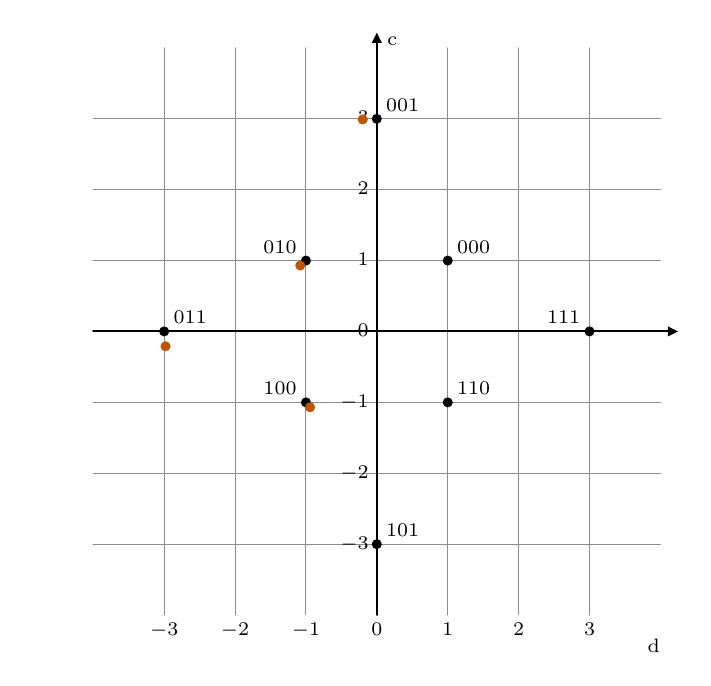
\begin{tikzpicture}[x=0.01600cm,y=-0.01600cm,line cap=round,line join=round]
\useasboundingbox (0,0) rectangle (520,500);
\path[draw=black!45,line width=0.35pt] (108.3,466) -- (108.3,16);
\path[draw=black!45,line width=0.35pt] (164.5,466) -- (164.5,16);
\path[draw=black!45,line width=0.35pt] (220.8,466) -- (220.8,16);
\path[draw=black!45,line width=0.35pt] (277,466) -- (277,16);
\path[draw=black!45,line width=0.35pt] (333.3,466) -- (333.3,16);
\path[draw=black!45,line width=0.35pt] (389.5,466) -- (389.5,16);
\path[draw=black!45,line width=0.35pt] (445.8,466) -- (445.8,16);
\path[draw=black!45,line width=0.35pt] (52,409.8) -- (502,409.8);
\path[draw=black!45,line width=0.35pt] (52,353.5) -- (502,353.5);
\path[draw=black!45,line width=0.35pt] (52,297.3) -- (502,297.3);
\path[draw=black!45,line width=0.35pt] (52,241) -- (502,241);
\path[draw=black!45,line width=0.35pt] (52,184.8) -- (502,184.8);
\path[draw=black!45,line width=0.35pt] (52,128.5) -- (502,128.5);
\path[draw=black!45,line width=0.35pt] (52,72.3) -- (502,72.3);
\path[draw=black,line width=0.7pt] (52,241) -- (510,241);
\path[fill=black,draw=none] (516,241) -- (508,237) -- (508,245) -- cycle;
\path[draw=black,line width=0.7pt] (277,466) -- (277,10);
\path[fill=black,draw=none] (277,4) -- (273,12) -- (281,12) -- cycle;
\node[anchor=base,inner sep=0pt,font=\scriptsize] at (108.3,482) {$-$3};
\node[anchor=base,inner sep=0pt,font=\scriptsize] at (164.5,482) {$-$2};
\node[anchor=base,inner sep=0pt,font=\scriptsize] at (220.8,482) {$-$1};
\node[anchor=base,inner sep=0pt,font=\scriptsize] at (277,482) {0};
\node[anchor=base,inner sep=0pt,font=\scriptsize] at (333.3,482) {1};
\node[anchor=base,inner sep=0pt,font=\scriptsize] at (389.5,482) {2};
\node[anchor=base,inner sep=0pt,font=\scriptsize] at (445.8,482) {3};
\node[anchor=base east,inner sep=0pt,font=\scriptsize] at (271,413.8) {$-$3};
\node[anchor=base east,inner sep=0pt,font=\scriptsize] at (271,357.5) {$-$2};
\node[anchor=base east,inner sep=0pt,font=\scriptsize] at (271,301.3) {$-$1};
\node[anchor=base east,inner sep=0pt,font=\scriptsize] at (271,245) {0};
\node[anchor=base east,inner sep=0pt,font=\scriptsize] at (271,188.8) {1};
\node[anchor=base east,inner sep=0pt,font=\scriptsize] at (271,132.5) {2};
\node[anchor=base east,inner sep=0pt,font=\scriptsize] at (271,76.3) {3};
\node[anchor=base east,inner sep=0pt,font=\scriptsize] at (502,496) {d};
\node[anchor=base west,inner sep=0pt,font=\scriptsize] at (285,14) {c};
\path[fill=black,draw=none] (333.3,184.8) circle[radius=0.064cm];
\node[anchor=base west,inner sep=0pt,font=\scriptsize] at (340.3,178.8) {000};
\path[fill=black,draw=none] (277,72.3) circle[radius=0.064cm];
\node[anchor=base west,inner sep=0pt,font=\scriptsize] at (284,66.3) {001};
\path[fill=black,draw=none] (220.8,184.8) circle[radius=0.064cm];
\node[anchor=base east,inner sep=0pt,font=\scriptsize] at (213.8,178.8) {010};
\path[fill=black,draw=none] (108.3,241) circle[radius=0.064cm];
\node[anchor=base west,inner sep=0pt,font=\scriptsize] at (115.3,235) {011};
\path[fill=black,draw=none] (220.8,297.3) circle[radius=0.064cm];
\node[anchor=base east,inner sep=0pt,font=\scriptsize] at (213.8,291.3) {100};
\path[fill=black,draw=none] (277,409.8) circle[radius=0.064cm];
\node[anchor=base west,inner sep=0pt,font=\scriptsize] at (284,403.8) {101};
\path[fill=black,draw=none] (333.3,297.3) circle[radius=0.064cm];
\node[anchor=base west,inner sep=0pt,font=\scriptsize] at (340.3,291.3) {110};
\path[fill=black,draw=none] (445.8,241) circle[radius=0.064cm];
\node[anchor=base east,inner sep=0pt,font=\scriptsize] at (438.8,235) {111};
\path[fill=cB,draw=none] (265.8,72.8) circle[radius=0.064cm];
\path[fill=cB,draw=none] (224.1,301.2) circle[radius=0.064cm];
\path[fill=cB,draw=none] (216.3,188.7) circle[radius=0.064cm];
\path[fill=cB,draw=none] (109.4,252.8) circle[radius=0.064cm];
\end{tikzpicture}\end{center}
\begin{itemize}
\item Kék pontok: az ideális tribitek. Piros pontok: a vett értékek, mind kb. 4\textdegree{}-kal az óramutatóval ellentétesen elfordulva, ugyanazon a sugáron.
\end{itemize}
\end{rajz}
\begin{tipp}[A gyűjtemény megoldása]
A gyűjtemény (gépelt „Megoldás”) szerint „a fázishiba nagy: $\tan^{-1}(-1{,}08/0{,}93)=130{,}73^{\circ}\ne145^{\circ}$”.
\end{tipp}
\begin{figyelem}[Javítás]
A fázishiba kicsi, kb. 4\textdegree{}: a gyűjtemény felcserélte a tengelyeket és rossz síknegyedet vett.
\end{figyelem}
\begin{eredmeny}

\begin{center}\adjustbox{max width=\linewidth}{$\displaystyle \text{b) }001\ 100\ 010\ 011\qquad\text{c) }k\approx1\qquad\text{d) }\Delta\varphi\approx4^{\circ}\qquad\text{e) a zaj elhanyagolható}$}\end{center}
\end{eredmeny}


% ------------------------------------------------------------------
\section{\texorpdfstring{7.8. feladat: 64-QAM fázis- és erősítéstűrése}{7.8. feladat: 64-QAM fázis- és erősítéstűrése}}\label{ai7_08}
\setcounter{lepes}{0}
\begin{feladat}{7.8. feladat}
Mekkora a 64-QAM ($\pm1\ldots\pm7$ rács) megengedett fázis-, erősítés- és csillapításhibája zajmentes esetben?

{\footnotesize\sffamily Forrás: ALL-IN 127. oldal $\cdot$ aiD\_7\_11 d). Címkék: vizsga, javítás}
\end{feladat}
\begin{keresunk}
\begin{itemize}
\item $\varphi_{\max}$ (a megengedett fázishiba), a megengedett erősítés és csillapítás
\end{itemize}
\end{keresunk}
\begin{jeloles}
\begin{jeltabla}
$\varphi_{\max}$ & a megengedett fázishiba & \emph{keresett}\\
$\varphi$ & fázishiba & \\
$k$ & erősítési tényező & \\
\end{jeltabla}
\par\smallskip\textbf{Adott még:}
\begin{itemize}
\item szintek $\pm1,\pm3,\pm5,\pm7$, határok $0,\pm2,\pm4,\pm6$
\end{itemize}
\end{jeloles}

\lepes{Fázis a sarokpontnál}
A $(7,7)$ pont szöge 45\textdegree{}, távolsága $7\sqrt2=9{,}9$. Elfordulva egyik koordinátája $9{,}9\cos(45^{\circ}+\varphi)$, ennek a 6-os határ felett kell maradnia.

\begin{center}\adjustbox{max width=\linewidth}{$\displaystyle \cos(45^{\circ}+\varphi)=\frac{6}{7\sqrt2}=0{,}606\ \Rightarrow\ 45^{\circ}+\varphi=52{,}7^{\circ}\ \Rightarrow\ \varphi=7{,}7^{\circ}$}\end{center}
\jegyzet{geometria}{}

\begin{center}\adjustbox{max width=\linewidth}{$\displaystyle (7,5):\ 7{,}8^{\circ}\qquad(7,3):\ 8{,}0^{\circ}\qquad(7,1):\ 8{,}1^{\circ}$}\end{center}
\jegyzet{ellenőrzés}{a többi pont kicsit többet tűr}

\lepes{Amplitúdó}
Csillapításnál a 7-es szint ér le a 6-os határra, erősítésnél az 5-ös ér fel a 6-osra.

\begin{center}\adjustbox{max width=\linewidth}{$\displaystyle 7k>6\ \Rightarrow\ k>\frac67=0{,}857\qquad5k<6\ \Rightarrow\ k<\frac65=1{,}2$}\end{center}
\jegyzet{számérték}{}
\begin{figyelem}[Javítás]
A gyűjtemény 9,46\textdegree{}-ot ad: ez a (7,7) és a (7,5) pont közötti szög, nem a döntési határig mért.
\end{figyelem}
\begin{eredmeny}

\begin{center}\adjustbox{max width=\linewidth}{$\displaystyle \varphi_{\max}\approx7{,}7^{\circ}\qquad\text{csillapítás legfeljebb }14{,}3\%,\ \text{erősítés legfeljebb }20\%$}\end{center}
\end{eredmeny}


% ------------------------------------------------------------------
\section{\texorpdfstring{7.9. feladat: 36-QAM négyzetrácson}{7.9. feladat: 36-QAM négyzetrácson}}\label{ai7_09}
\setcounter{lepes}{0}
\begin{feladat}{7.9. feladat}
36-féle szimbólum, négyzetrács. a) Konstelláció. b) A négyzetrács előnye. c) Erősítés- és csillapítástűrés zajmentesen. d) Egy kolléga a sarokpontokat a tengelyek mellé tenné. Mi javul, mi romlik?

{\footnotesize\sffamily Forrás: ALL-IN 128\ldots{}129. oldal $\cdot$ aiD\_7\_16 (és 5-ösöm 7. oldal). Címkék: vizsga, javítás}
\end{feladat}
\begin{keresunk}
\begin{itemize}
\item a) konstelláció
\item b) előny
\item c) tűrések
\item d) a sarokpontok áthelyezése
\end{itemize}
\end{keresunk}
\begin{jeloles}
\begin{jeltabla}
$\ca{M}$ & a konstelláció pontjainak száma & $6$\\
$k$ & erősítési tényező & \\
$\varphi$ & fázishiba & \\
$\varphi_{\max}$ & a megengedett fázishiba & \\
\end{jeltabla}
\end{jeloles}

\lepes{a) Konstelláció}
$36=6\times6$: tengelyenként 6 szint, egyenlő (2 egységnyi) közökkel, a nullára szimmetrikusan. A döntési határok a szintek között félúton vannak.

\begin{center}\adjustbox{max width=\linewidth}{$\displaystyle \text{szintek: }\pm1,\pm3,\pm5\qquad\text{határok: }0,\pm2,\pm4$}\end{center}
\jegyzet{definíció}{}

\lepes{b) Előny}
A két koordinátáról egymástól függetlenül, egyszerű küszöbökkel lehet dönteni: két hatszintű PAM-döntés.

\lepes{c) Amplitúdótűrés}
Csillapításnál az 5-ös szint ér le a 4-es határra, erősítésnél a 3-as ér fel a 4-esre.

\begin{center}\adjustbox{max width=\linewidth}{$\displaystyle 5k>4\Rightarrow k>0{,}8\ (-20\%)\qquad3k<4\Rightarrow k<1{,}33\ (+33\%)$}\end{center}
\jegyzet{számérték}{}

\lepes{c) Fázistűrés}
A sarokpont $(5,5)$, távolsága $5\sqrt2$.

\begin{center}\adjustbox{max width=\linewidth}{$\displaystyle 5\sqrt2\cos(45^{\circ}+\varphi)=4\ \Rightarrow\ \varphi=10{,}6^{\circ}$}\end{center}
\jegyzet{geometria}{$(5,1)$: 11,3\textdegree{}, $(5,3)$: 10,9\textdegree{}}

\lepes{d) Áthelyezés (7,1)-re}


\begin{center}\adjustbox{max width=\linewidth}{$\displaystyle \sqrt{5^2+5^2}=\sqrt{1^2+7^2}=5\sqrt2$}\end{center}
\jegyzet{ellenőrzés}{a teljesítmény nem csökken}

\begin{center}\adjustbox{max width=\linewidth}{$\displaystyle \mathrm{arctg}\tfrac17=8{,}1^{\circ}<10{,}6^{\circ}$}\end{center}
\jegyzet{geometria}{a fázistűrés romlik}

\begin{rajz}
\textbf{36-QAM konstelláció a döntési határokkal}\par
\begin{center}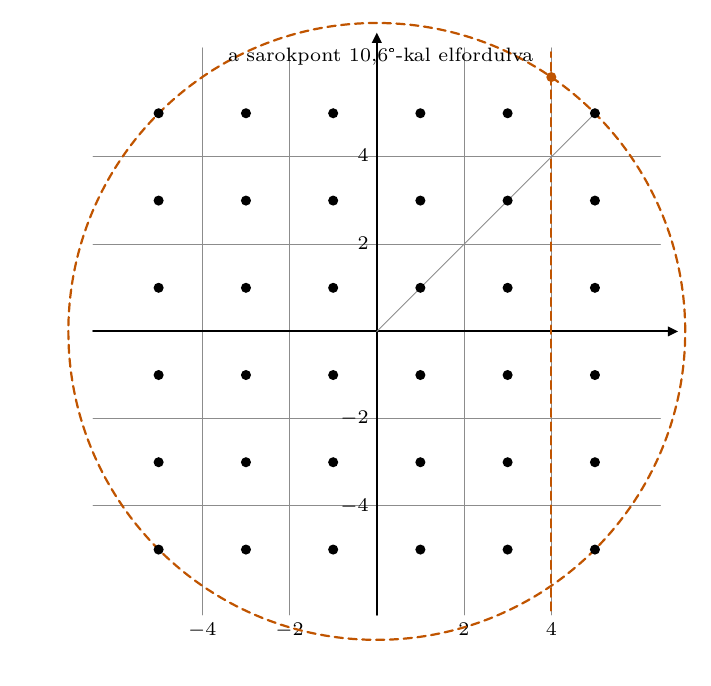
\begin{tikzpicture}[x=0.01600cm,y=-0.01600cm,line cap=round,line join=round]
\useasboundingbox (0,0) rectangle (520,500);
\path[draw=black!45,line width=0.35pt] (138.5,466) -- (138.5,16);
\path[draw=black!45,line width=0.35pt] (207.8,466) -- (207.8,16);
\path[draw=black!45,line width=0.35pt] (346.2,466) -- (346.2,16);
\path[draw=black!45,line width=0.35pt] (415.5,466) -- (415.5,16);
\path[draw=black!45,line width=0.35pt] (52,379.5) -- (502,379.5);
\path[draw=black!45,line width=0.35pt] (52,310.2) -- (502,310.2);
\path[draw=black!45,line width=0.35pt] (52,171.8) -- (502,171.8);
\path[draw=black!45,line width=0.35pt] (52,102.5) -- (502,102.5);
\path[draw=black,line width=0.7pt] (52,241) -- (510,241);
\path[fill=black,draw=none] (516,241) -- (508,237) -- (508,245) -- cycle;
\path[draw=black,line width=0.7pt] (277,466) -- (277,10);
\path[fill=black,draw=none] (277,4) -- (273,12) -- (281,12) -- cycle;
\node[anchor=base,inner sep=0pt,font=\scriptsize] at (138.5,482) {$-$4};
\node[anchor=base,inner sep=0pt,font=\scriptsize] at (207.8,482) {$-$2};
\node[anchor=base,inner sep=0pt,font=\scriptsize] at (346.2,482) {2};
\node[anchor=base,inner sep=0pt,font=\scriptsize] at (415.5,482) {4};
\node[anchor=base east,inner sep=0pt,font=\scriptsize] at (271,383.5) {$-$4};
\node[anchor=base east,inner sep=0pt,font=\scriptsize] at (271,314.2) {$-$2};
\node[anchor=base east,inner sep=0pt,font=\scriptsize] at (271,175.8) {2};
\node[anchor=base east,inner sep=0pt,font=\scriptsize] at (271,106.5) {4};
\path[draw=black!45,line width=0.35pt] (277,241) -- (450.1,67.9);
\path[draw=cB,line width=0.8pt,dash pattern=on 3pt off 2pt] (415.5,462.5) -- (415.5,19.5);
\path[draw=cB,line width=0.8pt,dash pattern=on 3pt off 2pt] (277,241) ellipse[x radius=3.917cm,y radius=3.917cm];
\path[fill=black,draw=none] (103.9,414.1) circle[radius=0.064cm];
\path[fill=black,draw=none] (103.9,344.8) circle[radius=0.064cm];
\path[fill=black,draw=none] (103.9,275.6) circle[radius=0.064cm];
\path[fill=black,draw=none] (103.9,206.4) circle[radius=0.064cm];
\path[fill=black,draw=none] (103.9,137.2) circle[radius=0.064cm];
\path[fill=black,draw=none] (103.9,67.9) circle[radius=0.064cm];
\path[fill=black,draw=none] (173.2,414.1) circle[radius=0.064cm];
\path[fill=black,draw=none] (173.2,344.8) circle[radius=0.064cm];
\path[fill=black,draw=none] (173.2,275.6) circle[radius=0.064cm];
\path[fill=black,draw=none] (173.2,206.4) circle[radius=0.064cm];
\path[fill=black,draw=none] (173.2,137.2) circle[radius=0.064cm];
\path[fill=black,draw=none] (173.2,67.9) circle[radius=0.064cm];
\path[fill=black,draw=none] (242.4,414.1) circle[radius=0.064cm];
\path[fill=black,draw=none] (242.4,344.8) circle[radius=0.064cm];
\path[fill=black,draw=none] (242.4,275.6) circle[radius=0.064cm];
\path[fill=black,draw=none] (242.4,206.4) circle[radius=0.064cm];
\path[fill=black,draw=none] (242.4,137.2) circle[radius=0.064cm];
\path[fill=black,draw=none] (242.4,67.9) circle[radius=0.064cm];
\path[fill=black,draw=none] (311.6,414.1) circle[radius=0.064cm];
\path[fill=black,draw=none] (311.6,344.8) circle[radius=0.064cm];
\path[fill=black,draw=none] (311.6,275.6) circle[radius=0.064cm];
\path[fill=black,draw=none] (311.6,206.4) circle[radius=0.064cm];
\path[fill=black,draw=none] (311.6,137.2) circle[radius=0.064cm];
\path[fill=black,draw=none] (311.6,67.9) circle[radius=0.064cm];
\path[fill=black,draw=none] (380.8,414.1) circle[radius=0.064cm];
\path[fill=black,draw=none] (380.8,344.8) circle[radius=0.064cm];
\path[fill=black,draw=none] (380.8,275.6) circle[radius=0.064cm];
\path[fill=black,draw=none] (380.8,206.4) circle[radius=0.064cm];
\path[fill=black,draw=none] (380.8,137.2) circle[radius=0.064cm];
\path[fill=black,draw=none] (380.8,67.9) circle[radius=0.064cm];
\path[fill=black,draw=none] (450.1,414.1) circle[radius=0.064cm];
\path[fill=black,draw=none] (450.1,344.8) circle[radius=0.064cm];
\path[fill=black,draw=none] (450.1,275.6) circle[radius=0.064cm];
\path[fill=black,draw=none] (450.1,206.4) circle[radius=0.064cm];
\path[fill=black,draw=none] (450.1,137.2) circle[radius=0.064cm];
\path[fill=black,draw=none] (450.1,67.9) circle[radius=0.064cm];
\path[fill=cB,draw=none] (415.5,39.2) circle[radius=0.064cm];
\node[anchor=base east,inner sep=0pt,font=\scriptsize] at (401.6,27) {a sarokpont 10,6\textdegree{}-kal elfordulva};
\end{tikzpicture}\end{center}
\begin{itemize}
\item $6\times6$ pont a $\pm1$, $\pm3$, $\pm5$ koordinátákon, a döntési határok (rács) a 0, $\pm2$, $\pm4$ értékeknél.
\item A sarokpont $(5,5)$ a legmesszebb van, $5\sqrt2$ sugarú körön mozog elforduláskor. 10,6\textdegree{}-nál éri el a 4-es határt (piros szaggatott).
\end{itemize}
\end{rajz}
\begin{figyelem}[Javítás]
A gyűjtemény fázistűrése asin(1/5) = 11,5\textdegree{}: az (5,1) pontot vizsgálta, a sarokpontot nem. A d) részben szerinte a fázistűrés nem változik, valójában 8,1\textdegree{}-ra romlik.
\end{figyelem}
\begin{eredmeny}

\begin{center}\adjustbox{max width=\linewidth}{$\displaystyle \text{c) }-20\%\ldots+33\%,\ \varphi_{\max}=10{,}6^{\circ}\qquad\text{d) itt nincs előnye, a fázistűrés romlik}$}\end{center}
\end{eredmeny}


% ------------------------------------------------------------------
\section{\texorpdfstring{7.10. feladat: Kevesebb teljesítmény 64-QAM-mel, azonos hibaaránnyal}{7.10. feladat: Kevesebb teljesítmény 64-QAM-mel, azonos hibaaránnyal}}\label{ai7_10}
\setcounter{lepes}{0}
\begin{feladat}{7.10. feladat}
64-QAM-nél azonos hibaarány mellett csökkenteni kell a teljesítményt. Adjon tippeket!

{\footnotesize\sffamily Forrás: ALL-IN 124. oldal $\cdot$ aiD\_7\_4 (és 5-ösöm 8. oldal). Címkék: beugró}
\end{feladat}
\begin{keresunk}
\begin{itemize}
\item ötletek
\end{itemize}
\end{keresunk}
\begin{jeloles}
\begin{jeltabla}
$d$ & egy pont távolsága az origótól & \\
\end{jeltabla}
\par\smallskip\textbf{Adott még:}
\begin{itemize}
\item $8\times8$-as rács, a hibaarányt a legkisebb távolság (2) szabja meg
\end{itemize}
\end{jeloles}

\lepes{Hol a teljesítmény?}
A pont teljesítménye $d^2$.

\begin{center}\adjustbox{max width=\linewidth}{$\displaystyle \overline{d^2}=2\cdot\frac{1+9+25+49}{4}=42\qquad d^2_{(7,7)}=98$}\end{center}
\jegyzet{számérték}{a sarokpont több mint kétszerese az átlagnak}

\lepes{Ötletek}
A sarokpontokat beljebb kell húzni üres rácshelyekre, a 2-es legkisebb távolságot megtartva: kereszt vagy közel kör alakú konstelláció. Ugyanakkora hibaarányt kisebb teljesítmény mellett ad hibajavító kódolás (kódolási nyereség), kisebb zajú vevő vagy nagyobb antennanyereség is.
\begin{eredmeny}

\begin{center}\adjustbox{max width=\linewidth}{$\displaystyle \text{sarokpontok beljebb (kör vagy kereszt alak), illetve hibajavító kód}$}\end{center}
\end{eredmeny}
\begin{tipp}[Ellenőrzés]
\begin{itemize}
\item A gyűjteményben „64$\times$64-es mátrix” áll, helyesen 8$\times$8-as rács.
\end{itemize}
\end{tipp}


% ------------------------------------------------------------------
\section{\texorpdfstring{7.11. feladat: Szemábra és 16-QAM: két feleletválasztós}{7.11. feladat: Szemábra és 16-QAM: két feleletválasztós}}\label{ai7_11}
\setcounter{lepes}{0}
\begin{feladat}{7.11. feladat}
a) Négyszintű PAM szemábrája, a szemek közepe 0,35 és 1,05 ms-nál: A) ISI-mentes elemi jel B) jelzési idő 0,7 ms C) RZ jel D) bitsebesség = 4 $\cdot$ szimbólumsebesség. b) 16-QAM: A) 4 időrés alatt 1 bit B) 1 időrés alatt 16 bit C) egyszerre 2 bit D) 100 kbaud mellett 400 kbit/s.

{\footnotesize\sffamily Forrás: ALL-IN 125. oldal $\cdot$ aiD\_7\_5 (3.1.), aiD\_7\_6 (4.3.). Címkék: beugró}
\end{feladat}
\begin{keresunk}
\begin{itemize}
\item melyik állítás igaz
\end{itemize}
\end{keresunk}
\begin{jeloles}
\begin{jeltabla}
$T$ & jelzési (bit-) idő & \\
$v$ & bitsebesség & \\
\end{jeltabla}
\par\smallskip\textbf{Adott még:}
\begin{itemize}
\item a) négyszintű PAM, két szomszédos szem közepe 0,35 és 1,05 ms
\item b) 16-QAM
\end{itemize}
\end{jeloles}

\lepes{a) Szemábra}
Két szomszédos szem közepe között egy jelzési idő telik el. Nyitott, éles szem a mintavételi pillanatban ISI-mentes elemi jelre utal. Négy szintnél egy szimbólum $\log_24=2$ bit.

\begin{center}\adjustbox{max width=\linewidth}{$\displaystyle T=1{,}05-0{,}35=0{,}7\ \text{ms}$}\end{center}
\jegyzet{számérték}{B igaz}

\begin{center}\adjustbox{max width=\linewidth}{$\displaystyle v=2\cdot\frac1T$}\end{center}
\jegyzet{definíció}{D hamis (2-szeres, nem 4-szeres)}

\lepes{b) 16-QAM}
Egy szimbólum $\log_216=4$ bit.

\begin{center}\adjustbox{max width=\linewidth}{$\displaystyle 100\ \text{kBd}\cdot4=400\ \text{kbit/s}$}\end{center}
\jegyzet{definíció}{csak D igaz}
\begin{eredmeny}

\begin{center}\adjustbox{max width=\linewidth}{$\displaystyle \text{a) A és B}\qquad\text{b) D}$}\end{center}
\end{eredmeny}
\begin{tipp}[Ellenőrzés]
\begin{itemize}
\item a) A és C a saját olvasatom, a gyűjteményben nincs jelölve \texttt{[ELLENŐRIZENDŐ]}.
\end{itemize}
\end{tipp}


% ------------------------------------------------------------------
\section{\texorpdfstring{7.12. feladat: QAM-16, [160,100] kód, 20 MHz (Moodle 2020)}{7.12. feladat: QAM-16, [160,100] kód, 20 MHz (Moodle 2020)}}\label{ai7_12}
\setcounter{lepes}{0}
\begin{feladat}{7.12. feladat}
QAM-16, emelt koszinuszos elemi spektrum, [160,100] hibadetektáló kód, a teljes sáv 20 MHz. Mekkora a nettó bitsebesség?

{\footnotesize\sffamily Forrás: ALL-IN 13. oldal $\cdot$ ai2020\_06\_02\_Q4. Címkék: vizsga, javítás}
\end{feladat}
\begin{keresunk}
\begin{itemize}
\item nettó bitsebesség
\end{itemize}
\end{keresunk}
\begin{jeloles}
\begin{jeltabla}
$\ca{B}$ & a rendelkezésre álló sávszélesség & $20$\,MHz\\
$\alpha$ & lekerekítési tényező & \\
$T$ & jelzési (bit-) idő & \\
\end{jeltabla}
\par\smallskip\textbf{Adott még:}
\begin{itemize}
\item 16-QAM: 4 bit/szimbólum
\item $\alpha$ (lekerekítési tényező) nincs megadva
\end{itemize}
\end{jeloles}

\lepes{Szimbólumsebesség}
Vivőfrekvenciás emelt koszinuszos jel: ${\ca{B}}=(1+\alpha)/T$, tehát $1/T={\ca{B}}/(1+\alpha)$.

\begin{center}\adjustbox{max width=\linewidth}{$\displaystyle \alpha=1:\ \frac1T=\frac{20}{2}=10\ \text{MBd}\qquad\alpha=0:\ \frac1T={\ca{20}}\ \text{MBd}$}\end{center}
\jegyzet{tétel}{}

\lepes{Nettó bitsebesség}
Szimbólumsebesség $\times$ 4 bit $\times$ kódarány.

\begin{center}\adjustbox{max width=\linewidth}{$\displaystyle \alpha=1:\ 10\cdot4\cdot0{,}625=25\ \text{Mbit/s}$}\end{center}
\jegyzet{számérték}{}

\begin{center}\adjustbox{max width=\linewidth}{$\displaystyle \alpha=0:\ {\ca{20}}\cdot4\cdot0{,}625=50\ \text{Mbit/s}$}\end{center}
\jegyzet{számérték}{elméleti felső korlát}
\begin{figyelem}[Javítás]
A hallgató a sávszélesség-képletet rosszul rendezte át (40 MBd, 100 Mbit/s). A javító 0 + 1 pontot adott. Az $\alpha$ értékét a feladat nem adja meg \texttt{[ELLENŐRIZENDŐ]}.
\end{figyelem}
\begin{eredmeny}

\begin{center}\adjustbox{max width=\linewidth}{$\displaystyle 25\ \text{Mbit/s}\ (\alpha=1)\qquad\text{legfeljebb }50\ \text{Mbit/s}\ (\alpha=0)$}\end{center}
\end{eredmeny}


% ------------------------------------------------------------------
\section{\texorpdfstring{7.13. feladat: 150 Mbit/s 72 MHz-ben: 8-PSK vagy 16-QAM?}{7.13. feladat: 150 Mbit/s 72 MHz-ben: 8-PSK vagy 16-QAM?}}\label{ai7_13}
\setcounter{lepes}{0}
\begin{feladat}{7.13. feladat}
Adatsebesség 150 Mbit/s, sáv 72 MHz. a) Megoldható-e 8-PSK-val? b) Mivel lehetne? c) Miért nem akármilyen nagy $n$-QAM-mel?

{\footnotesize\sffamily Forrás: ALL-IN 22. oldal $\cdot$ ai2016\_01\_05\_8. Címkék: vizsga, javítás}
\end{feladat}
\begin{keresunk}
\begin{itemize}
\item a) 8-PSK
\item b) más moduláció
\item c) indoklás
\end{itemize}
\end{keresunk}
\begin{jeloles}
\begin{jeltabla}
$\ca{v}$ & bitsebesség & $150$\,Mbit/s\\
$\cb{B}$ & a rendelkezésre álló sávszélesség & $72$\,MHz\\
$n$ & a QAM-konstelláció pontjainak száma & \\
$T$ & jelzési (bit-) idő & \\
$\alpha$ & lekerekítési tényező & \\
\end{jeltabla}
\end{jeloles}

\lepes{a) 8-PSK}
$\log_28=3$ bit/szimbólum. A sávkorlátból a megengedett lekerekítés:

\begin{center}\adjustbox{max width=\linewidth}{$\displaystyle \frac1T=\frac{150}{3}=50\ \text{MBd}$}\end{center}
\jegyzet{számérték}{}

\begin{center}\adjustbox{max width=\linewidth}{$\displaystyle (1+\alpha)\cdot50\le{\cb{72}}\ \Rightarrow\ \alpha\le0{,}44$}\end{center}
\jegyzet{tétel}{megoldható, ha a szűrő elég meredek}

\lepes{b) 16-QAM}
4 bit/szimbólum.

\begin{center}\adjustbox{max width=\linewidth}{$\displaystyle \frac1T=37{,}5\ \text{MBd}\qquad(1+\alpha)\cdot37{,}5\le{\cb{72}}\ \Rightarrow\ \alpha\le0{,}92$}\end{center}
\jegyzet{számérték}{kényelmesen belefér}

\lepes{c) Miért nem akármekkora?}
Azonos teljesítménynél a több pont sűrűbben van: csökken a zaj-, erősítés- és fázistűrés, egyre nagyobb jel-zaj viszony kell.
\begin{figyelem}[Javítás]
A hallgató szerint 8-PSK-val nem megy. Ez csak $\alpha=1$-re igaz, a feladat nem rögzíti az $\alpha$-t \texttt{[ELLENŐRIZENDŐ]}.
\end{figyelem}
\begin{eredmeny}

\begin{center}\adjustbox{max width=\linewidth}{$\displaystyle \text{a) igen, ha }\alpha\le0{,}44\qquad\text{b) 16-QAM, }\alpha\le0{,}92\qquad\text{c) romlik a zajtűrés}$}\end{center}
\end{eredmeny}

% Generálva: html/build_tex.js (ai08.js). Kézzel ne szerkeszd, a forrás a html/data mappa.
\setcounter{chapter}{7}
\chapter{\texorpdfstring{Hang, hallás, kép, látás}{Hang, hallás, kép, látás}}\label{f8}
Decibel és phon különbsége, a hallásküszöb frekvenciafüggése, valamint a színes kép világossági jele. Rövid, de pontos fogalmakat kérnek.

\section{Alapok, egyszerűen}
\subsection{\texorpdfstring{A1. Jelölések, hangnyomásszint és hangosság}{A1. Jelölések, hangnyomásszint és hangosság}}\label{a8-hang}
\par\noindent{\small\renewcommand{\arraystretch}{1.25}\begin{tabularx}{\linewidth}{@{}>{\raggedright\arraybackslash}X>{\raggedright\arraybackslash}X@{}}\toprule
\textbf{Jel} & \textbf{Jelentés}\\\midrule
undefined, undefined & hangnyomás (effektív érték), és a 1 kHz-es hallásküszöb: undefined \textmu{}Pa\\
undefined, undefined & hangintenzitás (W/m\textsuperscript{2}), a küszöbhöz tartozó undefined W/m\textsuperscript{2}\\
undefined & hangnyomásszint (dB)\\
undefined & hangosságszint (phon)\\
\bottomrule\end{tabularx}}\par

\begin{center}\adjustbox{max width=\linewidth}{$\displaystyle L=20\lg\frac{p}{p_0}=10\lg\frac{I}{I_0}$}\end{center}

A két alak azért egyezik, mert az intenzitás a nyomás négyzetével arányos. A \textbf{phon} a hangosságérzet egysége: egy hang annyi phon, ahány dB-es az azonos hangosnak érzett 1 kHz-es szinusz. 1 kHz-en a phon és a dB megegyezik, az éppen hallható hang minden frekvencián 0 phon. Mély frekvencián a fül érzéketlenebb (100 Hz-en a küszöb kb. 25 dB, 400 Hz-en kb. 10 dB).

Pontforrás szabad térben: az intenzitás $1/r^2$-tel csökken, tízszeres távolságon 20 dB-lel kisebb a szint.

\subsection{\texorpdfstring{A2. Világossági jel és színkülönbségi jelek}{A2. Világossági jel és színkülönbségi jelek}}\label{a8-kep}
$R$, $G$, $B$: a vörös, zöld, kék színjel (0 és 1 között). A világossági jel a szem érzékenységével súlyozott összeg:

\begin{center}\adjustbox{max width=\linewidth}{$\displaystyle Y=0{,}3R+0{,}59G+0{,}11B\qquad C_b\propto B-Y,\ C_r\propto R-Y$}\end{center}

Azonos intenzitásnál a fekete-fehér képen a zöld a legvilágosabb, a kék a legsötétebb. A láthatósági függvény $V(\lambda)$ a szem relatív érzékenysége, maximuma 1 (normált), nappali látásnál 555 nm-nél.

% ------------------------------------------------------------------
\section{\texorpdfstring{8.1. feladat: Hangsugárzó: 1 W-tal 93 dB (Moodle 2020)}{8.1. feladat: Hangsugárzó: 1 W-tal 93 dB (Moodle 2020)}}\label{ai8_01}
\setcounter{lepes}{0}
\begin{feladat}{8.1. feladat}
1 W, 1 kHz, 1 m-re 93 dB. a) Mekkora teljesítmény kell a fájdalomküszöbhöz? b) A mikrofon helyén hány phon az a) esetben? c) Miért mérhető 100 Hz-en azonos teljesítménnyel 109 dB?

{\footnotesize\sffamily Forrás: ALL-IN 5. oldal $\cdot$ ai2020\_05\_26\_Q5. Címkék: vizsga, javítás}
\end{feladat}
\begin{keresunk}
\begin{itemize}
\item a) $P$ (elektromos teljesítmény)
\item b) $L_N$ (hangosságszint (phon))
\item c) indoklás
\end{itemize}
\end{keresunk}
\begin{jeloles}
\begin{jeltabla}
$P$ & elektromos teljesítmény & \emph{keresett}\\
$L_N$ & hangosságszint (phon) & \emph{keresett}\\
\end{jeltabla}
\par\smallskip\textbf{Adott még:}
\begin{itemize}
\item 1 W elektromos teljesítménnyel 1 kHz-en 1 m-re 93 dB
\item fájdalomküszöb: 120 dB (egyes források 123 dB)
\end{itemize}
\end{jeloles}

\lepes{a) Teljesítmény}
A szint a teljesítménnyel $10\lg$ szerint nő (azonos frekvencián és helyen). 93 dB-ről 120 dB-re 27 dB kell.

\begin{center}\adjustbox{max width=\linewidth}{$\displaystyle 10\lg\frac{P}{1\ \text{W}}=120-93=27\ \Rightarrow\ P=10^{2{,}7}\ \text{W}\approx500\ \text{W}$}\end{center}
\jegyzet{behelyettesítés}{123 dB-es küszöbbel $10^3=1000$ W}

\lepes{b) Phon}
1 kHz-en a phon egyenlő a dB-lel (A1).

\begin{center}\adjustbox{max width=\linewidth}{$\displaystyle L_N=120\ \text{phon}$}\end{center}
\jegyzet{definíció}{az a) esetben}

\lepes{c) 100 Hz}
A dB fizikai mennyiség, nem érzet. Azonos elektromos teljesítményre a hangszóró (és a mikrofon) más-más hangnyomást ad különböző frekvenciákon: az átvitelük frekvenciafüggő. Itt 100 Hz-en 16 dB-lel hatékonyabban sugároz. Hangosságban viszont a 109 dB 100 Hz-en kevesebb phon, mert ott érzéketlenebb a fül.
\begin{figyelem}[Javítás]
A b) válasza 93 phon volt: ez a kiinduló helyzetre igaz, az a) esetre a fájdalomküszöb phonértéke a helyes. A javító teljes pontot adott, a 123 dB-es feltevést is elfogadta, mert le volt írva.
\end{figyelem}
\begin{eredmeny}

\begin{center}\adjustbox{max width=\linewidth}{$\displaystyle \text{a) }\approx500\ \text{W}\qquad\text{b) }120\ \text{phon}\qquad\text{c) a hangszóró és a mikrofon frekvenciafüggése}$}\end{center}
\end{eredmeny}


% ------------------------------------------------------------------
\section{\texorpdfstring{8.2. feladat: Függvénygenerátor és hangszóró: hány phon?}{8.2. feladat: Függvénygenerátor és hangszóró: hány phon?}}\label{ai8_02}
\setcounter{lepes}{0}
\begin{feladat}{8.2. feladat}
Az éppen hallható 10 kHz-es hang 10 (illetve 15) dB, ugyanazzal az amplitúdóval 1 kHz-en 30 dB, 100 Hz-en 0 dB. a) A 10 kHz-es hang hangossága? b) Az 1 kHz-esé? c) A 100 Hz-esé? d) Miért mások a szintek azonos amplitúdónál?

{\footnotesize\sffamily Forrás: ALL-IN 82\ldots{}83., 135. oldal $\cdot$ ai2014\_01\_14\_4, aiD\_8\_9 (és 5-ösöm 21. oldal). Címkék: vizsga}
\end{feladat}
\begin{keresunk}
\begin{itemize}
\item a), b), c) hangosságszint phonban
\item d) indoklás
\end{itemize}
\end{keresunk}
\begin{jeloles}
\par\smallskip\textbf{Adott még:}
\begin{itemize}
\item 10 kHz: 10 (15) dB, éppen hallható
\item 1 kHz: 30 dB
\item 100 Hz: 0 dB
\end{itemize}
\end{jeloles}

\lepes{a) 10 kHz}
Az éppen hallható hang definíció szerint 0 phon.

\begin{center}\adjustbox{max width=\linewidth}{$\displaystyle 0\ \text{phon}$}\end{center}
\jegyzet{definíció}{}

\lepes{b) 1 kHz}
1 kHz-en phon = dB.

\begin{center}\adjustbox{max width=\linewidth}{$\displaystyle 30\ \text{dB}\ \Rightarrow\ 30\ \text{phon}$}\end{center}
\jegyzet{definíció}{}

\lepes{c) 100 Hz}
100 Hz-en a hallásküszöb kb. 25 dB.

\begin{center}\adjustbox{max width=\linewidth}{$\displaystyle 0\ \text{dB}<25\ \text{dB}$}\end{center}
\jegyzet{ellenőrzés}{nem hallható}

\lepes{d) Miért mások?}
Ugyanaz a generátorfeszültség a hangszóró frekvenciafüggő átvitele miatt más-más hangnyomást ad.
\begin{eredmeny}

\begin{center}\adjustbox{max width=\linewidth}{$\displaystyle \text{a) }0\ \text{phon}\qquad\text{b) }30\ \text{phon}\qquad\text{c) nem hallható}\qquad\text{d) a hangszóró frekvenciafüggése}$}\end{center}
\end{eredmeny}
\begin{tipp}[Ellenőrzés]
\begin{itemize}
\item c) A gyűjtemény szerint „0 dB a légköri nyomás”: helyesen a 20 \textmu{}Pa-os referencia-hangnyomás.
\end{itemize}
\end{tipp}


% ------------------------------------------------------------------
\section{\texorpdfstring{8.3. feladat: A hallásküszöb 1000-szeres és 100-szoros hangnyomása}{8.3. feladat: A hallásküszöb 1000-szeres és 100-szoros hangnyomása}}\label{ai8_03}
\setcounter{lepes}{0}
\begin{feladat}{8.3. feladat}
Hány phon az 1 kHz-es szinusz, amelynek hangnyomása a hallásküszöbhöz tartozó a) 1000-szerese, b) 100-szorosa? Hány dB, mennyire érezzük hangosnak?

{\footnotesize\sffamily Forrás: ALL-IN 136. oldal $\cdot$ aiD\_8\_14, aiD\_8\_15 (hivatalos). Címkék: beugró}
\end{feladat}
\begin{keresunk}
\begin{itemize}
\item $L$ dB-ben (hangnyomásszint) és phonban
\end{itemize}
\end{keresunk}
\begin{jeloles}
\begin{jeltabla}
$\ca{p}$ & hangnyomás & $1000$\\
$p_0$ & a hallásküszöb hangnyomása & \\
$L$ & hangnyomásszint & \emph{keresett}\\
\end{jeltabla}
\end{jeloles}

\lepes{Számolás}
Nyomásarányból $20\lg$ (A1), 1 kHz-en phon = dB.

\begin{center}\adjustbox{max width=\linewidth}{$\displaystyle a)\ 20\lg{\ca{1000}}=60\ \text{dB}=60\ \text{phon}\qquad b)\ 20\lg100=40\ \text{dB}=40\ \text{phon}$}\end{center}
\jegyzet{definíció}{}
\begin{eredmeny}

\begin{center}\adjustbox{max width=\linewidth}{$\displaystyle \text{a) }60\ \text{phon (iroda, vendéglő)}\qquad\text{b) }40\ \text{phon (csendes lakás, éjjel)}$}\end{center}
\end{eredmeny}


% ------------------------------------------------------------------
\section{\texorpdfstring{8.4. feladat: 120 dB-hez mekkora hangnyomás kell?}{8.4. feladat: 120 dB-hez mekkora hangnyomás kell?}}\label{ai8_04}
\setcounter{lepes}{0}
\begin{feladat}{8.4. feladat}
A hallásküszöb 20 \textmu{}Pa, 120 dB-es tartományban hallunk. Mekkora nyomású „zavar” kell a tartomány tetejéhez?

{\footnotesize\sffamily Forrás: ALL-IN 134. oldal $\cdot$ aiD\_8\_5. Címkék: beugró}
\end{feladat}
\begin{keresunk}
\begin{itemize}
\item $p_1$ (a keresett hangnyomás)
\end{itemize}
\end{keresunk}
\begin{jeloles}
\begin{jeltabla}
$\ca{p_0}$ & a hallásküszöb hangnyomása & $20$\,\textmu{}Pa\\
$\cb{L}$ & hangnyomásszint & $120$\,dB\\
$p_1$ & a keresett hangnyomás & \emph{keresett}\\
\end{jeltabla}
\end{jeloles}

\lepes{Számolás}
${\cb{L}}={\ca{20}}\lg(p_1/{\ca{p_0}})$-ból kifejezzük $p_1$-et. ${\ca{20}}\lg$, mert nyomásról (amplitúdó jellegű mennyiségről) van szó.

\begin{center}\adjustbox{max width=\linewidth}{$\displaystyle \frac{p_1}{p_0}=10^{120/{\ca{20}}}=10^6\ \Rightarrow\ p_1=10^6\cdot{\ca{20}}\ \mu\text{Pa}={\ca{20}}\ \text{Pa}$}\end{center}
\jegyzet{átalakítás}{a légköri nyomás ($10^5$ Pa) ötezred része}
\begin{eredmeny}

\begin{center}\adjustbox{max width=\linewidth}{$\displaystyle p_1=20\ \text{Pa}$}\end{center}
\end{eredmeny}


% ------------------------------------------------------------------
\section{\texorpdfstring{8.5. feladat: 100 Hz, 1 nW/m\textsuperscript{2}}{8.5. feladat: 100 Hz, 1 nW/m²}}\label{ai8_05}
\setcounter{lepes}{0}
\begin{feladat}{8.5. feladat}
Milyen hangos a 100 Hz-es, 1 nW/m\textsuperscript{2} intenzitású szinusz? A) 1000 phon B) 30 phon. Hány dB a szintje? C) 20 dB D) 30 dB

{\footnotesize\sffamily Forrás: ALL-IN 134. oldal $\cdot$ aiD\_8\_8 (4.2.). Címkék: beugró}
\end{feladat}
\begin{keresunk}
\begin{itemize}
\item $L$ (hangnyomásszint) és $L_N$ (hangosságszint (phon))
\end{itemize}
\end{keresunk}
\begin{jeloles}
\begin{jeltabla}
$\ca{I}$ & hangintenzitás & $10$\,W/m\\
$\cb{f}$ & frekvencia & $100$\,Hz\\
$L$ & hangnyomásszint & \emph{keresett}\\
$L_N$ & hangosságszint (phon) & \emph{keresett}\\
\end{jeltabla}
\end{jeloles}

\lepes{A szint}
Intenzitásból $10\lg$ (A1).

\begin{center}\adjustbox{max width=\linewidth}{$\displaystyle L=10\lg\frac{10^{-9}}{10^{-12}}=10\lg1000=30\ \text{dB}$}\end{center}
\jegyzet{definíció}{D igaz, C hamis}

\lepes{A hangosság}
100 Hz-en a küszöb kb. 25 dB, így a 30 dB alig van felette: néhány phon. 30 phon csak 1 kHz-en lenne. Az 1000 phon értelmetlen.

\begin{center}\adjustbox{max width=\linewidth}{$\displaystyle L_N\ll30\ \text{phon}$}\end{center}
\jegyzet{ellenőrzés}{A és B hamis}
\begin{eredmeny}

\begin{center}\adjustbox{max width=\linewidth}{$\displaystyle \text{csak D igaz: }30\ \text{dB, néhány phon}$}\end{center}
\end{eredmeny}


% ------------------------------------------------------------------
\section{\texorpdfstring{8.6. feladat: 400 Hz vagy 1 kHz: melyik hangosabb?}{8.6. feladat: 400 Hz vagy 1 kHz: melyik hangosabb?}}\label{ai8_06}
\setcounter{lepes}{0}
\begin{feladat}{8.6. feladat}
a) 400 Hz 20 phon vagy 1 kHz 20 phon? b) 400 Hz 20 dB vagy 1 kHz 20 dB?

{\footnotesize\sffamily Forrás: ALL-IN 133. oldal $\cdot$ aiD\_8\_2. Címkék: beugró}
\end{feladat}
\begin{keresunk}
\begin{itemize}
\item melyik hangosabb
\end{itemize}
\end{keresunk}
\begin{jeloles}
\begin{jeltabla}
$L_N$ & hangosságszint (phon) & \\
\end{jeltabla}
\par\smallskip\textbf{Adott még:}
\begin{itemize}
\item két hang, a) phonban, b) dB-ben megadva
\end{itemize}
\end{jeloles}

\lepes{a) Phonban}
A phon definíció szerint az érzett hangosság: azonos phon azonos hangosság.

\begin{center}\adjustbox{max width=\linewidth}{$\displaystyle 20\ \text{phon}=20\ \text{phon}$}\end{center}
\jegyzet{definíció}{egyformák}

\lepes{b) dB-ben}
1 kHz-en a 20 dB 20 phon. 400 Hz-en a küszöb kb. 10 dB, ezért a 20 dB ott kevesebb, kb. 12 és 15 phon közötti hangosság.

\begin{center}\adjustbox{max width=\linewidth}{$\displaystyle L_N(400\ \text{Hz},\ 20\ \text{dB})<20\ \text{phon}$}\end{center}
\jegyzet{közelítés}{az 1 kHz-es hangosabb}
\begin{eredmeny}

\begin{center}\adjustbox{max width=\linewidth}{$\displaystyle \text{a) egyformák}\qquad\text{b) az 1 kHz-es}$}\end{center}
\end{eredmeny}
\begin{tipp}[Ellenőrzés]
\begin{itemize}
\item A gyűjtemény b) indoklása („a 400 Hz-es 20 dB a küszöb alatt van”) nem igaz, a következtetés jó. A küszöbértéket az izofon-ábráról kell venni \texttt{[ELLENŐRIZENDŐ]}.
\end{itemize}
\end{tipp}


% ------------------------------------------------------------------
\section{\texorpdfstring{8.7. feladat: Elromlott mikrofon: 2 m-en 30 dB, a terem végén?}{8.7. feladat: Elromlott mikrofon: 2 m-en 30 dB, a terem végén?}}\label{ai8_07}
\setcounter{lepes}{0}
\begin{feladat}{8.7. feladat}
2 m-re az előadótól 30 dB. a) Körülbelül mennyi a terem végén (20 m)? b) Mi befolyásolja, hogy hátul hallják-e?

{\footnotesize\sffamily Forrás: ALL-IN 88. oldal $\cdot$ ai2016\_01\_12c\_6. Címkék: vizsga}
\end{feladat}
\begin{keresunk}
\begin{itemize}
\item a) $L_2$ (a szint a második helyen)
\item b) indoklás
\end{itemize}
\end{keresunk}
\begin{jeloles}
\begin{jeltabla}
$\ca{L_1}$ & a szint az első helyen & $30$\,dB\\
$\cb{r_1}$ & a forrástól mért távolság & $2$\,m\\
$\cc{r_2}$ & a forrástól mért távolság & $20$\,m\\
$L_2$ & a szint a második helyen & \emph{keresett}\\
$I$ & hangintenzitás & \\
$r$ & a forrástól mért távolság & \\
$L$ & hangnyomásszint & \\
\end{jeltabla}
\end{jeloles}

\lepes{a) Távolságtörvény}
Pontforrás szabad térben: $I\propto1/r^2$, ezért a szint ${\cc{20}}\lg$ szerint csökken a távolsággal.

\begin{center}\adjustbox{max width=\linewidth}{$\displaystyle \Delta L=10\lg\frac{r_2^2}{r_1^2}={\cc{20}}\lg\frac{20}{2}={\cc{20}}\ \text{dB}$}\end{center}
\jegyzet{tétel}{}

\begin{center}\adjustbox{max width=\linewidth}{$\displaystyle L_2={\ca{30}}-{\cc{20}}=10\ \text{dB}$}\end{center}
\jegyzet{számérték}{}

\lepes{b) Mi befolyásolja?}
Zárt teremben a visszaverődések (zengő tér) miatt a csökkenés kisebb. Döntő a háttérzaj (elfedés), a terem akusztikája, és hogy 10 dB-en a beszéd mély és magas összetevői a hallásküszöb alatt vannak.
\begin{eredmeny}

\begin{center}\adjustbox{max width=\linewidth}{$\displaystyle \text{a) }\approx10\ \text{dB}\qquad\text{b) háttérzaj, teremakusztika, a hallásküszöb frekvenciafüggése}$}\end{center}
\end{eredmeny}


% ------------------------------------------------------------------
\section{\texorpdfstring{8.8. feladat: Színsávok fekete-fehér TV-n és RGB-hármasok világossága}{8.8. feladat: Színsávok fekete-fehér TV-n és RGB-hármasok világossága}}\label{ai8_08}
\setcounter{lepes}{0}
\begin{feladat}{8.8. feladat}
a) Három egyforma intenzitású sáv: kék, zöld, vörös. Melyik a legsötétebb a fekete-fehér képen, és hogyan olvaszthatnánk össze két csíkot a zöld fényességével? b) Melyik kelti a legnagyobb világosságérzetet: $(0{,}1;\ 0;\ 0{,}1)$, $(0{,}3;\ 0{,}1;\ 0{,}3)$, $(0;\ 0{,}1;\ 0{,}1)$, $(0{,}4;\ 0{,}1;\ 0{,}2)$?

{\footnotesize\sffamily Forrás: ALL-IN 134. oldal $\cdot$ aiD\_8\_4, aiD\_8\_7 (3.5.). Címkék: beugró}
\end{feladat}
\begin{keresunk}
\begin{itemize}
\item a) a legsötétebb sáv, és a zöld csökkentése
\item b) a legnagyobb $Y$ (világossági jel)
\end{itemize}
\end{keresunk}
\begin{jeloles}
\begin{jeltabla}
$\ca{Y}$ & világossági jel & $0{,}3$\\
$R$ & vörös színjel & \\
$G$ & zöld színjel & \\
$B$ & kék színjel & \\
$Y_G$ & a tiszta zöld sáv világossága & \\
$Y_R$ & a tiszta vörös sáv világossága & \\
$Y_B$ & a tiszta kék sáv világossága & \\
\end{jeltabla}
\par\smallskip\textbf{Adott még:}
\begin{itemize}
\item b) négy $(R;\ G;\ B)$ hármas
\end{itemize}
\end{jeloles}

\lepes{a) Fekete-fehér kép}
A fekete-fehér TV csak ${\ca{Y}}$-t mutatja. Egyforma intenzitásnál a súlyok döntenek.

\begin{center}\adjustbox{max width=\linewidth}{$\displaystyle Y_G=0{,}59>Y_R={\ca{0{,}3}}>Y_B=0{,}11$}\end{center}
\jegyzet{definíció}{a kék a legsötétebb}

\begin{center}\adjustbox{max width=\linewidth}{$\displaystyle 0{,}59\,G'={\ca{0{,}3}}\ \Rightarrow\ G'=0{,}51$}\end{center}
\jegyzet{átalakítás}{a zöldet kb. a felére csökkentve a vörössel egyforma szürke lesz}

\lepes{b) Világosság}
Mindegyikre kiszámoljuk ${\ca{Y}}$-t.

\begin{center}\adjustbox{max width=\linewidth}{$\displaystyle 0{,}03+0+0{,}011=0{,}041\qquad0{,}09+0{,}059+0{,}033=0{,}182$}\end{center}
\jegyzet{behelyettesítés}{}

\begin{center}\adjustbox{max width=\linewidth}{$\displaystyle 0+0{,}059+0{,}011=0{,}070\qquad0{,}12+0{,}059+0{,}022=0{,}201$}\end{center}
\jegyzet{behelyettesítés}{a negyedik a legnagyobb}
\begin{eredmeny}

\begin{center}\adjustbox{max width=\linewidth}{$\displaystyle \text{a) a kék a legsötétebb, a zöld}\times0{,}51\qquad\text{b) }(0{,}4;\ 0{,}1;\ 0{,}2),\ Y=0{,}201$}\end{center}
\end{eredmeny}


% ------------------------------------------------------------------
\section{\texorpdfstring{8.9. feladat: Primitív színes rendszer 2 és 1 bites RGB-vel (hivatalos)}{8.9. feladat: Primitív színes rendszer 2 és 1 bites RGB-vel (hivatalos)}}\label{ai8_09}
\setcounter{lepes}{0}
\begin{feladat}{8.9. feladat}
R, G, B egyenként 2 bites (0, 33, 67, 100\%). a) Hány színérzet? b) Hány fényességérték? c) Hány szürke? d) 1 bites színjelekkel sorolja fel a színeket fényesség szerint!

{\footnotesize\sffamily Forrás: ALL-IN 140\ldots{}141. oldal $\cdot$ aiD\_9\_7. Címkék: vizsga}
\end{feladat}
\begin{keresunk}
\begin{itemize}
\item a) színek száma
\item b) különböző $Y$ (világossági jel) értékek
\item c) szürkék
\item d) 1 bites színek $Y$ (világossági jel) szerint
\end{itemize}
\end{keresunk}
\begin{jeloles}
\begin{jeltabla}
$Y$ & világossági jel & \emph{keresett}\\
$R$ & vörös színjel & \\
$a$ & a vörös színjel szintjének sorszáma (0\ldots{}3) & \\
$G$ & zöld színjel & \\
$b$ & a zöld színjel szintjének sorszáma (0\ldots{}3) & \\
$B$ & kék színjel & \\
$c$ & a kék színjel szintjének sorszáma (0\ldots{}3) & \\
\end{jeltabla}
\par\smallskip\textbf{Adott még:}
\begin{itemize}
\item színjelenként 2 bit: 4 szint (0, 1/3, 2/3, 1)
\end{itemize}
\end{jeloles}

\lepes{a) Színek}
Három független jel, mindegyik 4 értékű.

\begin{center}\adjustbox{max width=\linewidth}{$\displaystyle 4^3=2^{3\cdot2}=64$}\end{center}
\jegyzet{számérték}{}

\lepes{b) Fényességértékek}
A négy szint $R=a/3$, $G=b/3$, $B=c/3$, ahol $a,b,c\in\{0,1,2,3\}$. Ezért $Y=0{,}3R+0{,}59G+0{,}11B=(30a+59b+11c)/3$ százalék. A 64 kombináció mind különböző $Y$-t ad (a 30, 59 és 11 súlyok miatt nincs két egyforma összeg).

\begin{center}\adjustbox{max width=\linewidth}{$\displaystyle 64\ \text{különböző }Y$}\end{center}
\jegyzet{ellenőrzés}{}

\lepes{c) Szürkék}
Szürke: $R=G=B$.

\begin{center}\adjustbox{max width=\linewidth}{$\displaystyle 0,\ 33,\ 67,\ 100\%:\ 4\ \text{szürke}$}\end{center}
\jegyzet{számérték}{}

\lepes{d) 1 bites színek}
Minden jel 0 vagy 1, $Y$ az összeadott súlyok.

\begin{center}\adjustbox{max width=\linewidth}{$\displaystyle 0,\ 11,\ 30,\ 41,\ 59,\ 70,\ 89,\ 100\%$}\end{center}
\jegyzet{számérték}{fekete, kék, vörös, bíbor, zöld, kékeszöld, sárga, fehér}
\begin{eredmeny}

\begin{center}\adjustbox{max width=\linewidth}{$\displaystyle \text{a) }64\quad\text{b) }64\quad\text{c) }4\quad\text{d) fekete}<\text{kék}<\text{vörös}<\text{bíbor}<\text{zöld}<\text{kékeszöld}<\text{sárga}<\text{fehér}$}\end{center}
\end{eredmeny}


% ------------------------------------------------------------------
\section{\texorpdfstring{8.10. feladat: Fogalmak: metamer szín, fúziós frekvencia, váltott sor, láthatóság}{8.10. feladat: Fogalmak: metamer szín, fúziós frekvencia, váltott sor, láthatóság}}\label{ai8_10}
\setcounter{lepes}{0}
\begin{feladat}{8.10. feladat}
a) Mi a metamer szín? b) Mi a látás fúziós frekvenciája? c) Mi a váltott soros képalkotás előnye? d) Rajzolja fel a láthatósági függvényt, mekkora a maximuma?

{\footnotesize\sffamily Forrás: ALL-IN 133., 135\ldots{}136. oldal $\cdot$ aiD\_8\_1, aiD\_8\_6, aiD\_8\_13, aiD\_8\_16 (és 5-ösöm 22\ldots{}23. oldal). Címkék: beugró, javítás}
\end{feladat}
\begin{keresunk}
\begin{itemize}
\item a), b), c), d) definíciók és indoklás
\end{itemize}
\end{keresunk}
\begin{jeloles}
\begin{jeltabla}
$V$ & láthatósági függvény, $V(\lambda)$ & \\
$\lambda$ & a fény hullámhossza & \\
\end{jeltabla}
\par\smallskip\textbf{Adott még:}
\begin{itemize}
\item fogalmi kérdések
\end{itemize}
\end{jeloles}

\lepes{a) Metamer szín}
Két különböző spektrális összetételű fény, amely azonos színérzetet kelt. A szem csak három csatornán (három csapfajtával) mér, ezért sokféle spektrum ad ugyanolyan hármast. Ezen alapul a háromszínes (RGB) képmegjelenítés.

\lepes{b) Fúziós frekvencia}
Az a villogási frekvencia (kb. 45 és 60 Hz között, fényerőfüggő), amely fölött a villogó fényt folyamatosnak látjuk. A mozgás folyamatosságához ennél kevesebb, 10\ldots{}20 kép/s is elég.

\lepes{c) Váltott soros képalkotás}
Egy kép két félképből áll (páratlan, majd páros sorok). 50 félkép/s villog, ez a fúziós frekvencia felett van, a sávszélesség viszont csak 25 teljes kép/s-é.

\lepes{d) Láthatósági függvény}
$V(\lambda)$ harang alakú, kb. 400 és 700 nm között számottevő, maximuma 1 (normált), nappali látásnál 555 nm-en (sárgászöld).

\begin{rajz}
\textbf{A láthatósági függvény (közelítő görbe)}\par
\begin{center}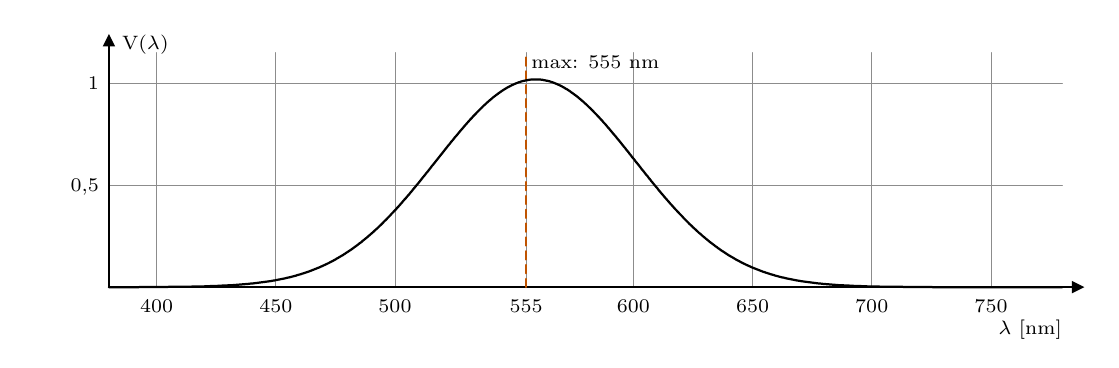
\begin{tikzpicture}[x=0.01985cm,y=-0.01985cm,line cap=round,line join=round]
\useasboundingbox (0,0) rectangle (680,200);
\path[draw=black!45,line width=0.35pt] (82.5,166) -- (82.5,16);
\path[draw=black!45,line width=0.35pt] (158.8,166) -- (158.8,16);
\path[draw=black!45,line width=0.35pt] (235,166) -- (235,16);
\path[draw=black!45,line width=0.35pt] (318.9,166) -- (318.9,16);
\path[draw=black!45,line width=0.35pt] (387.5,166) -- (387.5,16);
\path[draw=black!45,line width=0.35pt] (463.8,166) -- (463.8,16);
\path[draw=black!45,line width=0.35pt] (540,166) -- (540,16);
\path[draw=black!45,line width=0.35pt] (616.3,166) -- (616.3,16);
\path[draw=black!45,line width=0.35pt] (52,35.6) -- (662,35.6);
\path[draw=black!45,line width=0.35pt] (52,100.8) -- (662,100.8);
\path[draw=black,line width=0.7pt] (52,166) -- (670,166);
\path[fill=black,draw=none] (676,166) -- (668,162) -- (668,170) -- cycle;
\path[draw=black,line width=0.7pt] (52,166) -- (52,10);
\path[fill=black,draw=none] (52,4) -- (48,12) -- (56,12) -- cycle;
\node[anchor=base,inner sep=0pt,font=\scriptsize] at (82.5,182) {400};
\node[anchor=base,inner sep=0pt,font=\scriptsize] at (158.8,182) {450};
\node[anchor=base,inner sep=0pt,font=\scriptsize] at (235,182) {500};
\node[anchor=base,inner sep=0pt,font=\scriptsize] at (318.9,182) {555};
\node[anchor=base,inner sep=0pt,font=\scriptsize] at (387.5,182) {600};
\node[anchor=base,inner sep=0pt,font=\scriptsize] at (463.8,182) {650};
\node[anchor=base,inner sep=0pt,font=\scriptsize] at (540,182) {700};
\node[anchor=base,inner sep=0pt,font=\scriptsize] at (616.3,182) {750};
\node[anchor=base east,inner sep=0pt,font=\scriptsize] at (46,39.6) {1};
\node[anchor=base east,inner sep=0pt,font=\scriptsize] at (46,104.8) {0,5};
\node[anchor=base east,inner sep=0pt,font=\scriptsize] at (662,196) {$\lambda$ [nm]};
\node[anchor=base west,inner sep=0pt,font=\scriptsize] at (60,14) {V($\lambda$)};
\path[draw=cB,line width=0.8pt,dash pattern=on 3pt off 2pt] (318.9,166) -- (318.9,16);
\node[anchor=base west,inner sep=0pt,font=\scriptsize] at (321.9,26) {max: 555 nm};
\path[draw=black,line width=0.8pt] (52,166) -- (52.8,166) -- (53.5,166) -- (54.3,166) -- (55.1,166) -- (55.8,166) -- (56.6,166) -- (57.3,166) -- (58.1,166) -- (58.9,166) -- (59.6,166) -- (60.4,166) -- (61.2,166) -- (61.9,166) -- (62.7,166) -- (63.4,166) -- (64.2,166) -- (65,166) -- (65.7,166) -- (66.5,166) -- (67.3,166) -- (68,166) -- (68.8,166) -- (69.5,166) -- (70.3,166) -- (71.1,166) -- (71.8,165.9) -- (72.6,165.9) -- (73.4,165.9) -- (74.1,165.9) -- (74.9,165.9) -- (75.6,165.9) -- (76.4,165.9) -- (77.2,165.9) -- (77.9,165.9) -- (78.7,165.9) -- (79.5,165.9) -- (80.2,165.9) -- (81,165.9) -- (81.7,165.9) -- (82.5,165.9) -- (83.3,165.9) -- (84,165.9) -- (84.8,165.9) -- (85.6,165.9) -- (86.3,165.9) -- (87.1,165.9) -- (87.8,165.9) -- (88.6,165.9) -- (89.4,165.9) -- (90.1,165.8) -- (90.9,165.8) -- (91.7,165.8) -- (92.4,165.8) -- (93.2,165.8) -- (93.9,165.8) -- (94.7,165.8) -- (95.5,165.8) -- (96.2,165.8) -- (97,165.8) -- (97.8,165.8) -- (98.5,165.8) -- (99.3,165.7) -- (100,165.7) -- (100.8,165.7) -- (101.6,165.7) -- (102.3,165.7) -- (103.1,165.7) -- (103.9,165.7) -- (104.6,165.7) -- (105.4,165.6) -- (106.1,165.6) -- (106.9,165.6) -- (107.7,165.6) -- (108.4,165.6) -- (109.2,165.6) -- (110,165.5) -- (110.7,165.5) -- (111.5,165.5) -- (112.2,165.5) -- (113,165.5) -- (113.8,165.4) -- (114.5,165.4) -- (115.3,165.4) -- (116.1,165.4) -- (116.8,165.3) -- (117.6,165.3) -- (118.3,165.3) -- (119.1,165.3) -- (119.9,165.2) -- (120.6,165.2) -- (121.4,165.2) -- (122.2,165.1) -- (122.9,165.1) -- (123.7,165.1) -- (124.4,165) -- (125.2,165) -- (126,165) -- (126.7,164.9) -- (127.5,164.9) -- (128.3,164.8) -- (129,164.8) -- (129.8,164.8) -- (130.5,164.7) -- (131.3,164.7) -- (132.1,164.6) -- (132.8,164.6) -- (133.6,164.5) -- (134.4,164.5) -- (135.1,164.4) -- (135.9,164.3) -- (136.6,164.3) -- (137.4,164.2) -- (138.2,164.2) -- (138.9,164.1) -- (139.7,164) -- (140.5,164) -- (141.2,163.9) -- (142,163.8) -- (142.7,163.7) -- (143.5,163.7) -- (144.3,163.6) -- (145,163.5) -- (145.8,163.4) -- (146.6,163.3) -- (147.3,163.2) -- (148.1,163.1) -- (148.8,163) -- (149.6,162.9) -- (150.4,162.8) -- (151.1,162.7) -- (151.9,162.6) -- (152.7,162.5) -- (153.4,162.4) -- (154.2,162.3) -- (154.9,162.2) -- (155.7,162.1) -- (156.5,161.9) -- (157.2,161.8) -- (158,161.7) -- (158.8,161.5) -- (159.5,161.4) -- (160.3,161.2) -- (161,161.1) -- (161.8,160.9) -- (162.6,160.8) -- (163.3,160.6) -- (164.1,160.5) -- (164.9,160.3) -- (165.6,160.1) -- (166.4,159.9) -- (167.1,159.8) -- (167.9,159.6) -- (168.7,159.4) -- (169.4,159.2) -- (170.2,159) -- (171,158.8) -- (171.7,158.6) -- (172.5,158.3) -- (173.2,158.1) -- (174,157.9) -- (174.8,157.7) -- (175.5,157.4) -- (176.3,157.2) -- (177.1,156.9) -- (177.8,156.7) -- (178.6,156.4) -- (179.3,156.2) -- (180.1,155.9) -- (180.9,155.6) -- (181.6,155.3) -- (182.4,155) -- (183.2,154.7) -- (183.9,154.4) -- (184.7,154.1) -- (185.4,153.8) -- (186.2,153.5) -- (187,153.2) -- (187.7,152.8) -- (188.5,152.5) -- (189.3,152.1) -- (190,151.8) -- (190.8,151.4) -- (191.5,151.1) -- (192.3,150.7) -- (193.1,150.3) -- (193.8,149.9) -- (194.6,149.5) -- (195.4,149.1) -- (196.1,148.7) -- (196.9,148.3) -- (197.6,147.8) -- (198.4,147.4) -- (199.2,146.9) -- (199.9,146.5) -- (200.7,146) -- (201.5,145.6) -- (202.2,145.1) -- (203,144.6) -- (203.7,144.1) -- (204.5,143.6) -- (205.3,143.1) -- (206,142.6) -- (206.8,142.1) -- (207.6,141.5) -- (208.3,141) -- (209.1,140.4) -- (209.8,139.9) -- (210.6,139.3) -- (211.4,138.7) -- (212.1,138.1) -- (212.9,137.6) -- (213.7,137) -- (214.4,136.3) -- (215.2,135.7) -- (215.9,135.1) -- (216.7,134.5) -- (217.5,133.8) -- (218.2,133.2) -- (219,132.5) -- (219.8,131.8) -- (220.5,131.2) -- (221.3,130.5) -- (222,129.8) -- (222.8,129.1) -- (223.6,128.4) -- (224.3,127.7) -- (225.1,126.9) -- (225.9,126.2) -- (226.6,125.5) -- (227.4,124.7) -- (228.1,123.9) -- (228.9,123.2) -- (229.7,122.4) -- (230.4,121.6) -- (231.2,120.8) -- (232,120) -- (232.7,119.2) -- (233.5,118.4) -- (234.2,117.6) -- (235,116.8) -- (235.8,116) -- (236.5,115.1) -- (237.3,114.3) -- (238.1,113.4) -- (238.8,112.6) -- (239.6,111.7) -- (240.3,110.8) -- (241.1,109.9) -- (241.9,109.1) -- (242.6,108.2) -- (243.4,107.3) -- (244.2,106.4) -- (244.9,105.5) -- (245.7,104.6) -- (246.4,103.7) -- (247.2,102.7) -- (248,101.8) -- (248.7,100.9) -- (249.5,100) -- (250.3,99) -- (251,98.1) -- (251.8,97.1) -- (252.5,96.2) -- (253.3,95.2) -- (254.1,94.3) -- (254.8,93.3) -- (255.6,92.4) -- (256.4,91.4) -- (257.1,90.5) -- (257.9,89.5) -- (258.6,88.5) -- (259.4,87.6) -- (260.2,86.6) -- (260.9,85.7) -- (261.7,84.7) -- (262.5,83.7) -- (263.2,82.8) -- (264,81.8) -- (264.7,80.9) -- (265.5,79.9) -- (266.3,78.9) -- (267,78) -- (267.8,77) -- (268.5,76.1) -- (269.3,75.1) -- (270.1,74.2) -- (270.8,73.2) -- (271.6,72.3) -- (272.4,71.4) -- (273.1,70.4) -- (273.9,69.5) -- (274.7,68.6) -- (275.4,67.7) -- (276.2,66.8) -- (276.9,65.9) -- (277.7,65) -- (278.5,64.1) -- (279.2,63.2) -- (280,62.3) -- (280.8,61.4) -- (281.5,60.6) -- (282.3,59.7) -- (283,58.9) -- (283.8,58.1) -- (284.6,57.2) -- (285.3,56.4) -- (286.1,55.6) -- (286.9,54.8) -- (287.6,54) -- (288.4,53.2) -- (289.1,52.5) -- (289.9,51.7) -- (290.7,51) -- (291.4,50.2) -- (292.2,49.5) -- (293,48.8) -- (293.7,48.1) -- (294.5,47.4) -- (295.2,46.8) -- (296,46.1) -- (296.8,45.5) -- (297.5,44.8) -- (298.3,44.2) -- (299.1,43.6) -- (299.8,43) -- (300.6,42.5) -- (301.3,41.9) -- (302.1,41.4) -- (302.9,40.8) -- (303.6,40.3) -- (304.4,39.8) -- (305.2,39.3) -- (305.9,38.9) -- (306.7,38.4) -- (307.4,38) -- (308.2,37.6) -- (309,37.2) -- (309.7,36.8) -- (310.5,36.5) -- (311.3,36.1) -- (312,35.8) -- (312.8,35.5) -- (313.5,35.2) -- (314.3,34.9) -- (315.1,34.7) -- (315.8,34.4) -- (316.6,34.2) -- (317.4,34) -- (318.1,33.9) -- (318.9,33.7) -- (319.6,33.6) -- (320.4,33.4) -- (321.2,33.3) -- (321.9,33.2) -- (322.7,33.2) -- (323.5,33.1) -- (324.2,33.1) -- (325,33.1) -- (325.7,33.1) -- (326.5,33.1) -- (327.3,33.2) -- (328,33.2) -- (328.8,33.3) -- (329.6,33.4) -- (330.3,33.6) -- (331.1,33.7) -- (331.8,33.9) -- (332.6,34) -- (333.4,34.2) -- (334.1,34.4) -- (334.9,34.7) -- (335.7,34.9) -- (336.4,35.2) -- (337.2,35.5) -- (337.9,35.8) -- (338.7,36.1) -- (339.5,36.5) -- (340.2,36.8) -- (341,37.2) -- (341.8,37.6) -- (342.5,38) -- (343.3,38.4) -- (344,38.9) -- (344.8,39.3) -- (345.6,39.8) -- (346.3,40.3) -- (347.1,40.8) -- (347.8,41.4) -- (348.6,41.9) -- (349.4,42.5) -- (350.1,43) -- (350.9,43.6) -- (351.7,44.2) -- (352.4,44.8) -- (353.2,45.5) -- (354,46.1) -- (354.7,46.8) -- (355.5,47.4) -- (356.2,48.1) -- (357,48.8) -- (357.8,49.5) -- (358.5,50.2) -- (359.3,51) -- (360.1,51.7) -- (360.8,52.5) -- (361.6,53.2) -- (362.3,54) -- (363.1,54.8) -- (363.9,55.6) -- (364.6,56.4) -- (365.4,57.2) -- (366.2,58.1) -- (366.9,58.9) -- (367.7,59.7) -- (368.4,60.6) -- (369.2,61.4) -- (370,62.3) -- (370.7,63.2) -- (371.5,64.1) -- (372.3,65) -- (373,65.9) -- (373.8,66.8) -- (374.5,67.7) -- (375.3,68.6) -- (376.1,69.5) -- (376.8,70.4) -- (377.6,71.4) -- (378.4,72.3) -- (379.1,73.2) -- (379.9,74.2) -- (380.6,75.1) -- (381.4,76.1) -- (382.2,77) -- (382.9,78) -- (383.7,78.9) -- (384.5,79.9) -- (385.2,80.9) -- (386,81.8) -- (386.7,82.8) -- (387.5,83.7) -- (388.3,84.7) -- (389,85.7) -- (389.8,86.6) -- (390.6,87.6) -- (391.3,88.5) -- (392.1,89.5) -- (392.8,90.5) -- (393.6,91.4) -- (394.4,92.4) -- (395.1,93.3) -- (395.9,94.3) -- (396.7,95.2) -- (397.4,96.2) -- (398.2,97.1) -- (398.9,98.1) -- (399.7,99) -- (400.5,100) -- (401.2,100.9) -- (402,101.8) -- (402.8,102.7) -- (403.5,103.7) -- (404.3,104.6) -- (405,105.5) -- (405.8,106.4) -- (406.6,107.3) -- (407.3,108.2) -- (408.1,109.1) -- (408.8,109.9) -- (409.6,110.8) -- (410.4,111.7) -- (411.1,112.6) -- (411.9,113.4) -- (412.7,114.3) -- (413.4,115.1) -- (414.2,116) -- (415,116.8) -- (415.7,117.6) -- (416.5,118.4) -- (417.2,119.2) -- (418,120) -- (418.8,120.8) -- (419.5,121.6) -- (420.3,122.4) -- (421.1,123.2) -- (421.8,123.9) -- (422.6,124.7) -- (423.3,125.5) -- (424.1,126.2) -- (424.9,126.9) -- (425.6,127.7) -- (426.4,128.4) -- (427.2,129.1) -- (427.9,129.8) -- (428.7,130.5) -- (429.4,131.2) -- (430.2,131.8) -- (431,132.5) -- (431.7,133.2) -- (432.5,133.8) -- (433.3,134.5) -- (434,135.1) -- (434.8,135.7) -- (435.5,136.3) -- (436.3,137) -- (437.1,137.6) -- (437.8,138.1) -- (438.6,138.7) -- (439.4,139.3) -- (440.1,139.9) -- (440.9,140.4) -- (441.6,141) -- (442.4,141.5) -- (443.2,142.1) -- (443.9,142.6) -- (444.7,143.1) -- (445.5,143.6) -- (446.2,144.1) -- (447,144.6) -- (447.7,145.1) -- (448.5,145.6) -- (449.3,146) -- (450,146.5) -- (450.8,146.9) -- (451.6,147.4) -- (452.3,147.8) -- (453.1,148.3) -- (453.8,148.7) -- (454.6,149.1) -- (455.4,149.5) -- (456.1,149.9) -- (456.9,150.3) -- (457.7,150.7) -- (458.4,151.1) -- (459.2,151.4) -- (459.9,151.8) -- (460.7,152.1) -- (461.5,152.5) -- (462.2,152.8) -- (463,153.2) -- (463.8,153.5) -- (464.5,153.8) -- (465.3,154.1) -- (466,154.4) -- (466.8,154.7) -- (467.6,155) -- (468.3,155.3) -- (469.1,155.6) -- (469.9,155.9) -- (470.6,156.2) -- (471.4,156.4) -- (472.1,156.7) -- (472.9,156.9) -- (473.7,157.2) -- (474.4,157.4) -- (475.2,157.7) -- (476,157.9) -- (476.7,158.1) -- (477.5,158.3) -- (478.2,158.6) -- (479,158.8) -- (479.8,159) -- (480.5,159.2) -- (481.3,159.4) -- (482.1,159.6) -- (482.8,159.8) -- (483.6,159.9) -- (484.3,160.1) -- (485.1,160.3) -- (485.9,160.5) -- (486.6,160.6) -- (487.4,160.8) -- (488.2,160.9) -- (488.9,161.1) -- (489.7,161.2) -- (490.4,161.4) -- (491.2,161.5) -- (492,161.7) -- (492.7,161.8) -- (493.5,161.9) -- (494.3,162.1) -- (495,162.2) -- (495.8,162.3) -- (496.5,162.4) -- (497.3,162.5) -- (498.1,162.6) -- (498.8,162.7) -- (499.6,162.8) -- (500.4,162.9) -- (501.1,163) -- (501.9,163.1) -- (502.6,163.2) -- (503.4,163.3) -- (504.2,163.4) -- (504.9,163.5) -- (505.7,163.6) -- (506.5,163.7) -- (507.2,163.7) -- (508,163.8) -- (508.7,163.9) -- (509.5,164) -- (510.3,164) -- (511,164.1) -- (511.8,164.2) -- (512.6,164.2) -- (513.3,164.3) -- (514.1,164.3) -- (514.8,164.4) -- (515.6,164.5) -- (516.4,164.5) -- (517.1,164.6) -- (517.9,164.6) -- (518.7,164.7) -- (519.4,164.7) -- (520.2,164.8) -- (520.9,164.8) -- (521.7,164.8) -- (522.5,164.9) -- (523.2,164.9) -- (524,165) -- (524.8,165) -- (525.5,165) -- (526.3,165.1) -- (527,165.1) -- (527.8,165.1) -- (528.6,165.2) -- (529.3,165.2) -- (530.1,165.2) -- (530.9,165.3) -- (531.6,165.3) -- (532.4,165.3) -- (533.1,165.3) -- (533.9,165.4) -- (534.7,165.4) -- (535.4,165.4) -- (536.2,165.4) -- (537,165.5) -- (537.7,165.5) -- (538.5,165.5) -- (539.2,165.5) -- (540,165.5) -- (540.8,165.6) -- (541.5,165.6) -- (542.3,165.6) -- (543.1,165.6) -- (543.8,165.6) -- (544.6,165.6) -- (545.3,165.7) -- (546.1,165.7) -- (546.9,165.7) -- (547.6,165.7) -- (548.4,165.7) -- (549.2,165.7) -- (549.9,165.7) -- (550.7,165.7) -- (551.4,165.8) -- (552.2,165.8) -- (553,165.8) -- (553.7,165.8) -- (554.5,165.8) -- (555.3,165.8) -- (556,165.8) -- (556.8,165.8) -- (557.5,165.8) -- (558.3,165.8) -- (559.1,165.8) -- (559.8,165.8) -- (560.6,165.9) -- (561.3,165.9) -- (562.1,165.9) -- (562.9,165.9) -- (563.6,165.9) -- (564.4,165.9) -- (565.2,165.9) -- (565.9,165.9) -- (566.7,165.9) -- (567.4,165.9) -- (568.2,165.9) -- (569,165.9) -- (569.7,165.9) -- (570.5,165.9) -- (571.3,165.9) -- (572,165.9) -- (572.8,165.9) -- (573.6,165.9) -- (574.3,165.9) -- (575.1,165.9) -- (575.8,165.9) -- (576.6,165.9) -- (577.4,165.9) -- (578.1,165.9) -- (578.9,166) -- (579.7,166) -- (580.4,166) -- (581.2,166) -- (581.9,166) -- (582.7,166) -- (583.5,166) -- (584.2,166) -- (585,166) -- (585.8,166) -- (586.5,166) -- (587.3,166) -- (588,166) -- (588.8,166) -- (589.6,166) -- (590.3,166) -- (591.1,166) -- (591.9,166) -- (592.6,166) -- (593.4,166) -- (594.1,166) -- (594.9,166) -- (595.7,166) -- (596.4,166) -- (597.2,166) -- (598,166) -- (598.7,166) -- (599.5,166) -- (600.2,166) -- (601,166) -- (601.8,166) -- (602.5,166) -- (603.3,166) -- (604.1,166) -- (604.8,166) -- (605.6,166) -- (606.3,166) -- (607.1,166) -- (607.9,166) -- (608.6,166) -- (609.4,166) -- (610.2,166) -- (610.9,166) -- (611.7,166) -- (612.4,166) -- (613.2,166) -- (614,166) -- (614.7,166) -- (615.5,166) -- (616.3,166) -- (617,166) -- (617.8,166) -- (618.5,166) -- (619.3,166) -- (620.1,166) -- (620.8,166) -- (621.6,166) -- (622.4,166) -- (623.1,166) -- (623.9,166) -- (624.6,166) -- (625.4,166) -- (626.2,166) -- (626.9,166) -- (627.7,166) -- (628.4,166) -- (629.2,166) -- (630,166) -- (630.7,166) -- (631.5,166) -- (632.3,166) -- (633,166) -- (633.8,166) -- (634.6,166) -- (635.3,166) -- (636.1,166) -- (636.8,166) -- (637.6,166) -- (638.4,166) -- (639.1,166) -- (639.9,166) -- (640.7,166) -- (641.4,166) -- (642.2,166) -- (642.9,166) -- (643.7,166) -- (644.5,166) -- (645.2,166) -- (646,166) -- (646.8,166) -- (647.5,166) -- (648.3,166) -- (649,166) -- (649.8,166) -- (650.6,166) -- (651.3,166) -- (652.1,166) -- (652.9,166) -- (653.6,166) -- (654.4,166) -- (655.1,166) -- (655.9,166) -- (656.7,166) -- (657.4,166) -- (658.2,166) -- (659,166) -- (659.7,166) -- (660.5,166) -- (661.2,166) -- (662,166);
\end{tikzpicture}\end{center}
\begin{itemize}
\item Harang alakú görbe kb. 400 és 700 nm között, a maximuma 1 (normált) 555 nm-nél (sárgászöld). A rajz a szokásos Gauss-közelítés, alakra jó, pontos értékekre a CIE-táblázat a mérvadó.
\end{itemize}
\end{rajz}
\begin{figyelem}[Javítás]
A gyűjtemény c) válasza („a fél képet fele annyi idő alatt lehet felrakni”) nem mondja ki a lényeget: a sávszélesség változatlan, a villogás a fúziós frekvencia fölé kerül.
\end{figyelem}
\begin{eredmeny}

\begin{center}\adjustbox{max width=\linewidth}{$\displaystyle \text{a) azonos színérzet más spektrummal}\quad\text{b) kb. 50 Hz}\quad\text{c) kétszeres villogás azonos sávval}\quad\text{d) max. 1, 555 nm}$}\end{center}
\end{eredmeny}

% Generálva: html/build_tex.js (ai09.js). Kézzel ne szerkeszd, a forrás a html/data mappa.
\setcounter{chapter}{8}
\chapter{\texorpdfstring{Műsorszórás, sztereó FM, digitális TV}{Műsorszórás, sztereó FM, digitális TV}}\label{f9}
Szuperheterodin vevő (oszcillátor, tükörfrekvencia), az FM sztereó multiplex jel szerkezete, és a DVB-C, DVB-T bitsebesség-számítása.

\section{Alapok, egyszerűen}
\subsection{\texorpdfstring{A1. Szuperheterodin: oszcillátor és tükör}{A1. Szuperheterodin: oszcillátor és tükör}}\label{a9-szuper}
A vevő a venni kívánt $f_v$ jelet a helyi oszcillátor $f_\text{osc}$ jelével keveri (szorozza). A különbségi frekvencia az állandó \textbf{középfrekvencia}: $|f_v-f_\text{osc}|=f_\mathrm{KF}$. \textbf{Felső keverés:} $f_\text{osc}=f_v+f_\mathrm{KF}$, a tükör $f_v+2f_\mathrm{KF}$. \textbf{Alsó keverés:} $f_\text{osc}=f_v-f_\mathrm{KF}$, a tükör $|f_v-2f_\mathrm{KF}|$.

A \textbf{tükör} az a másik frekvencia, amely az oszcillátorral \textbf{szintén} $f_\mathrm{KF}$-et ad (az oszcillátor túloldalán). Csak a keverő előtti, hangolt bemeneti (RF) szűrő tudja csillapítani. A felső keverés előnye a kisebb relatív hangolási tartomány.

\subsection{\texorpdfstring{A2. FM sztereó multiplex}{A2. FM sztereó multiplex}}\label{a9-sztereo}
$L$, $R$: a bal és a jobb csatorna. A multiplex jel (az FM-modulátor bemenete):

\begin{itemize}
\item $M=L+R$ a 50 Hz és 15 kHz közötti sávban (ezt hallja a mono vevő),
\item 19 kHz-es pilotjel (a vevő ebből állítja elő a 38 kHz-et),
\item $S=L-R$ AM-DSB/SC-vel a 38 kHz-es, elnyomott segédvivőn: 23 és 53 kHz között,
\item RDS 57 kHz-en.
\end{itemize}

Egy csatornán megszólaló $f$ frekvenciájú hang $M$-ben és $S$-ben is megjelenik, így az összetevők: $f$, $38\pm f$ kHz és a pilot. A 15 kHz feletti hangot a bemeneti szűrő levágja.

\subsection{\texorpdfstring{A3. DVB-C és DVB-T bitsebesség}{A3. DVB-C és DVB-T bitsebesség}}\label{a9-dvb}
DVB-C (egyvivős QAM): $(1+\alpha)/T\le8$ MHz, bruttó $=\log_2M/T$, nettó $=$ bruttó $\cdot188/204$ (RS(204,188): 204 bájtból 188 a hasznos). DVB-T (OFDM): 6817 vivő, ebből 6048 hasznos, $T_0$ a hasznos szimbólumidő, $GI$ a védőintervallum aránya:

\begin{center}\adjustbox{max width=\linewidth}{$\displaystyle R_s=\frac{6048}{(1+GI)T_0}\qquad v_\text{nettó}=R_s\log_2M\cdot\text{FEC}\cdot\frac{188}{204}$}\end{center}

% ------------------------------------------------------------------
\section{\texorpdfstring{9.1. feladat: Felső keverés: 97,6 és 107 MHz}{9.1. feladat: Felső keverés: 97,6 és 107 MHz}}\label{ai9_01}
\setcounter{lepes}{0}
\begin{feladat}{9.1. feladat}
CCIR FM, $f_\mathrm{KF}=10{,}7$ MHz, felső keverés. Hová hangoljuk az oszcillátort, és hol a tükör, ha az adó a) 97,6 MHz, b) 107 MHz?

{\footnotesize\sffamily Forrás: ALL-IN 44., 66\ldots{}67., 74., 141. oldal $\cdot$ ai2016\_01\_12\_2, ai2014\_12\_22\_5, ai2014\_01\_07\_5, aiD\_9\_10 (és 5-ösöm 24. oldal). Címkék: vizsga}
\end{feladat}
\begin{keresunk}
\begin{itemize}
\item $f_\text{osc}$ (az oszcillátor frekvenciája), $f_t$ (tükörfrekvencia)
\end{itemize}
\end{keresunk}
\begin{jeloles}
\begin{jeltabla}
$f_\mathrm{KF}$ & középfrekvencia & \\
$\ca{f_v}$ & a venni kívánt adó frekvenciája & $97{,}6$\,MHz\\
$f_\text{osc}$ & az oszcillátor frekvenciája & \emph{keresett}\\
$f_t$ & tükörfrekvencia & \emph{keresett}\\
\end{jeltabla}
\end{jeloles}

\lepes{a) 97,6 MHz}
Az oszcillátor $f_\mathrm{KF}$-fel a vett frekvencia felett, a tükör még egyszer $f_\mathrm{KF}$-fel feljebb (A1).
\behely{\bh{\ca{f_v}}{\ca{97{,}6\un{MHz}}}}

\begin{center}\adjustbox{max width=\linewidth}{$\displaystyle f_\text{osc}={\ca{97{,}6}}+10{,}7=108{,}3\ \text{MHz}\qquad f_t=108{,}3+10{,}7=119\ \text{MHz}$}\end{center}
\jegyzet{behelyettesítés}{ellenőrzés: $119-108{,}3=10{,}7$}

\lepes{b) 107 MHz}


\begin{center}\adjustbox{max width=\linewidth}{$\displaystyle f_\text{osc}=117{,}7\ \text{MHz}\qquad f_t=128{,}4\ \text{MHz}$}\end{center}
\jegyzet{behelyettesítés}{}
\begin{eredmeny}

\begin{center}\adjustbox{max width=\linewidth}{$\displaystyle \text{a) }108{,}3\ \text{és}\ 119\ \text{MHz}\qquad\text{b) }117{,}7\ \text{és}\ 128{,}4\ \text{MHz}$}\end{center}
\end{eredmeny}


% ------------------------------------------------------------------
\section{\texorpdfstring{9.2. feladat: A teljes CCIR sáv (hivatalos megoldás)}{9.2. feladat: A teljes CCIR sáv (hivatalos megoldás)}}\label{ai9_02}
\setcounter{lepes}{0}
\begin{feladat}{9.2. feladat}
87,5\ldots{}108 MHz, KF 10,7 MHz. a) Felső keverésnél milyen sávban hangolható az oszcillátor? b) Hová a 94,8 MHz-hez? c) A tükre? d) Miért jó a 10,7 MHz?

{\footnotesize\sffamily Forrás: ALL-IN 138. oldal $\cdot$ aiD\_9\_4. Címkék: vizsga}
\end{feladat}
\begin{keresunk}
\begin{itemize}
\item a) az oszcillátor tartománya
\item b) $f_\text{osc}$ (az oszcillátor frekvenciája) a 94,8 MHz-hez
\item c) $f_t$ (tükörfrekvencia)
\item d) indoklás
\end{itemize}
\end{keresunk}
\begin{jeloles}
\begin{jeltabla}
$f_\mathrm{KF}$ & középfrekvencia & \\
$f_\text{osc}$ & az oszcillátor frekvenciája & \emph{keresett}\\
$f_t$ & tükörfrekvencia & \emph{keresett}\\
\end{jeltabla}
\par\smallskip\textbf{Adott még:}
\begin{itemize}
\item vételi sáv: 87,5 és 108 MHz között (20,5 MHz széles)
\end{itemize}
\end{jeloles}

\lepes{a) Tartomány}
A sáv két szélére:

\begin{center}\adjustbox{max width=\linewidth}{$\displaystyle 87{,}5+10{,}7=98{,}2\ \ldots\ 108+10{,}7=118{,}7\ \text{MHz}$}\end{center}
\jegyzet{behelyettesítés}{}

\lepes{b), c) 94,8 MHz}


\begin{center}\adjustbox{max width=\linewidth}{$\displaystyle f_\text{osc}=94{,}8+10{,}7=105{,}5\ \text{MHz}\qquad f_t=94{,}8+21{,}4=116{,}2\ \text{MHz}$}\end{center}
\jegyzet{behelyettesítés}{}

\lepes{d) Miért jó a 10,7 MHz?}
A legalsó adó tükre is a sáv fölé esik, mert $2f_\mathrm{KF}=21{,}4$ MHz nagyobb a sáv 20,5 MHz-es szélességénél. A tükrök sávjában (108,9 és 129,4 MHz között) nincs FM-műsor, egy rögzített sávszűrő elég.

\begin{center}\adjustbox{max width=\linewidth}{$\displaystyle 87{,}5+21{,}4=108{,}9>108$}\end{center}
\jegyzet{ellenőrzés}{}
\begin{eredmeny}

\begin{center}\adjustbox{max width=\linewidth}{$\displaystyle \text{a) }98{,}2\ldots118{,}7\ \text{MHz}\qquad\text{b) }105{,}5\ \text{MHz}\qquad\text{c) }116{,}2\ \text{MHz}\qquad\text{d) }2f_\mathrm{KF}>20{,}5\ \text{MHz}$}\end{center}
\end{eredmeny}


% ------------------------------------------------------------------
\section{\texorpdfstring{9.3. feladat: 24\ldots{}36 MHz, KF 18 MHz: felső vagy alsó keverés?}{9.3. feladat: 24…36 MHz, KF 18 MHz: felső vagy alsó keverés?}}\label{ai9_03}
\setcounter{lepes}{0}
\begin{feladat}{9.3. feladat}
A vételi sáv 24 és 36 MHz között van, a KF 18 MHz. a) Mekkora tartományt fog át az oszcillátor felső, illetve alsó keverésnél? Melyik jobb? b) Alsó keverésnél hová kell hangolni a 25,5 MHz-hez? c) A tükre, és mi vele a gond?

{\footnotesize\sffamily Forrás: ALL-IN 142. oldal $\cdot$ aiD\_9\_15 (és 5-ösöm 24. oldal). Címkék: vizsga, javítás}
\end{feladat}
\begin{keresunk}
\begin{itemize}
\item a) $f_\text{osc}$ (az oszcillátor frekvenciája) tartománya
\item b) $f_\text{osc}$ (az oszcillátor frekvenciája) alsó keverésnél
\item c) $f_t$ (tükörfrekvencia)
\end{itemize}
\end{keresunk}
\begin{jeloles}
\begin{jeltabla}
$\ca{f_v}$ & a venni kívánt adó frekvenciája & $24$\,MHz\\
$f_\mathrm{KF}$ & középfrekvencia & \\
$f_\text{osc}$ & az oszcillátor frekvenciája & \emph{keresett}\\
$f_t$ & tükörfrekvencia & \emph{keresett}\\
\end{jeltabla}
\end{jeloles}

\lepes{a) Hangolási tartomány}
Az oszcillátort annál könnyebb megépíteni, minél kisebb a legnagyobb és a legkisebb frekvencia aránya.

\begin{center}\adjustbox{max width=\linewidth}{$\displaystyle \text{felső: }42\ldots54\ \text{MHz},\ \tfrac{54}{42}=1{,}29\qquad\text{alsó: }6\ldots18\ \text{MHz},\ \tfrac{18}{6}=3$}\end{center}
\jegyzet{behelyettesítés}{a felső a jobb}

\lepes{b) Alsó keverés}


\begin{center}\adjustbox{max width=\linewidth}{$\displaystyle f_\text{osc}=25{,}5-18=7{,}5\ \text{MHz}$}\end{center}
\jegyzet{behelyettesítés}{}

\lepes{c) A tükör}
Az a frekvencia, amely 7,5 MHz-cel keverve szintén 18 MHz-et ad. Mivel $7{,}5<18$, ez csak az összegfrekvencián lehet: $f_t+7{,}5=18$.

\begin{center}\adjustbox{max width=\linewidth}{$\displaystyle f_t=|{\ca{f_v}}-2f_\mathrm{KF}|=|25{,}5-36|=10{,}5\ \text{MHz}$}\end{center}
\jegyzet{behelyettesítés}{ellenőrzés: $10{,}5+7{,}5=18$}

\lepes{c) A gond}
A tükrök a sáv bejárása közben 12 MHz és 0 között mozognak, ezeket egy hangolt bemeneti szűrőnek kell elnyomnia. Ráadásul a sáv tetején (36 MHz) az oszcillátor 18 MHz-en, pont a KF-en jár, és közvetlenül bejut a KF-erősítőbe. Felső keverésnél ($f_t=60\ldots72$ MHz) ezek a gondok nincsenek.
\begin{figyelem}[Javítás]
A gyűjtemény tükörként 33 MHz-et ad ($F+f_0$): ez a keverés összegfrekvenciája, $|33-7{,}5|=25{,}5\ne18$, a 33 MHz-ből nem lesz KF.
\end{figyelem}
\begin{eredmeny}

\begin{center}\adjustbox{max width=\linewidth}{$\displaystyle \text{a) felső: }42\ldots54\ \text{MHz, alsó: }6\ldots18\ \text{MHz, a felső a jobb}\qquad\text{b) }7{,}5\ \text{MHz}\qquad\text{c) }f_t=10{,}5\ \text{MHz}$}\end{center}
\end{eredmeny}


% ------------------------------------------------------------------
\section{\texorpdfstring{9.4. feladat: Műholdvevő: 10,7\ldots{}11,7 GHz-ből 1\ldots{}2 GHz}{9.4. feladat: Műholdvevő: 10,7…11,7 GHz-ből 1…2 GHz}}\label{ai9_04}
\setcounter{lepes}{0}
\begin{feladat}{9.4. feladat}
A 10,7\ldots{}11,7 GHz-es műholdas sávot egy állandó oszcillátorral az 1\ldots{}2 GHz-es beltéri sávba kell tenni. Adjon meg oszcillátorfrekvenciát, és hol van a tükrök sávja?

{\footnotesize\sffamily Forrás: ALL-IN 141. oldal $\cdot$ aiD\_9\_9 (hivatalos). Címkék: vizsga}
\end{feladat}
\begin{keresunk}
\begin{itemize}
\item $f_\text{osc}$ (az oszcillátor frekvenciája) és a tükrök sávja
\end{itemize}
\end{keresunk}
\begin{jeloles}
\begin{jeltabla}
$\ca{f_v}$ & a venni kívánt adó frekvenciája & $10{,}7$\,GHz\\
$f_\text{osc}$ & az oszcillátor frekvenciája & \emph{keresett}\\
$f_t$ & tükörfrekvencia & \\
\end{jeltabla}
\par\smallskip\textbf{Adott még:}
\begin{itemize}
\item kimenő (KF-)sáv: 1 és 2 GHz között
\end{itemize}
\end{jeloles}

\lepes{Alsó keverés (oszcillátor a sáv alatt)}
A sáv alja az 1 GHz-re, a teteje a 2 GHz-re kerüljön.
\behely{\bh{\ca{f_v}}{\ca{10{,}7\un{GHz}}}}

\begin{center}\adjustbox{max width=\linewidth}{$\displaystyle f_\text{osc}={\ca{10{,}7}}-1=11{,}7-2=9{,}7\ \text{GHz}$}\end{center}
\jegyzet{behelyettesítés}{}

\begin{center}\adjustbox{max width=\linewidth}{$\displaystyle f_t=f_\text{osc}-(1\ldots2)=7{,}7\ldots8{,}7\ \text{GHz}$}\end{center}
\jegyzet{behelyettesítés}{}

\lepes{Felső keverés (oszcillátor a sáv felett)}
Itt a sáv megfordul: 10,7 GHz-ből 2 GHz, 11,7-ből 1 GHz lesz.
\behely{\bh{\ca{f_v}}{\ca{10{,}7\un{GHz}}}}

\begin{center}\adjustbox{max width=\linewidth}{$\displaystyle f_\text{osc}={\ca{10{,}7}}+2=11{,}7+1=12{,}7\ \text{GHz}$}\end{center}
\jegyzet{behelyettesítés}{}

\begin{center}\adjustbox{max width=\linewidth}{$\displaystyle f_t=f_\text{osc}+(1\ldots2)=13{,}7\ldots14{,}7\ \text{GHz}$}\end{center}
\jegyzet{behelyettesítés}{}
\begin{eredmeny}

\begin{center}\adjustbox{max width=\linewidth}{$\displaystyle 9{,}7\ \text{GHz (tükrök }7{,}7\ldots8{,}7\ \text{GHz)}\qquad\text{vagy}\qquad12{,}7\ \text{GHz (tükrök }13{,}7\ldots14{,}7\ \text{GHz)}$}\end{center}
\end{eredmeny}
\begin{tipp}[Ellenőrzés]
\begin{itemize}
\item A gyakorlatban (LNB) a 9,75 GHz körüli alsó oszcillátor terjedt el, a sáv nem fordul meg.
\end{itemize}
\end{tipp}


% ------------------------------------------------------------------
\section{\texorpdfstring{9.5. feladat: A sztereó multiplex jel és egy-egy fütty}{9.5. feladat: A sztereó multiplex jel és egy-egy fütty}}\label{ai9_05}
\setcounter{lepes}{0}
\begin{feladat}{9.5. feladat}
a) Rajzolja fel a sztereó jelet az FM előtt! b) Milyen összetevők jelennek meg, ha valaki 440 Hz-et fütyül a bal mikrofonba? c) Ha a bal mikrofon 10 kHz-et vesz? d) Ha a jobb mikrofon 25 kHz-et?

{\footnotesize\sffamily Forrás: ALL-IN 45\ldots{}46., 139. oldal $\cdot$ ai2016\_01\_12\_2 c), aiD\_9\_5. Címkék: vizsga}
\end{feladat}
\begin{keresunk}
\begin{itemize}
\item b), c), d) a multiplex jel összetevői
\end{itemize}
\end{keresunk}
\begin{jeloles}
\begin{jeltabla}
$M$ & az összegjel (L+R) & \\
$S$ & a különbségi (L$-$R) jel & \\
\end{jeltabla}
\end{jeloles}

\lepes{a) A spektrum}
$M$: 0,05 és 15 kHz között, pilot 19 kHz-en, $S$ két oldalsávja 23 és 53 kHz között (a 38 kHz-es segédvivő elnyomva), RDS 57 kHz-en.

\lepes{b) 440 Hz balra}
Csak $L$-ben van, ezért $M=L+R$ és $S=L-R$ is tartalmazza. $S$ a 38 kHz körül két oldalsávot ad.

\begin{center}\adjustbox{max width=\linewidth}{$\displaystyle 0{,}44\ \text{kHz},\quad38\pm0{,}44=37{,}56\ \text{és}\ 38{,}44\ \text{kHz},\quad19\ \text{kHz (pilot)}$}\end{center}
\jegyzet{definíció}{}

\lepes{c) 10 kHz balra}


\begin{center}\adjustbox{max width=\linewidth}{$\displaystyle 10,\quad38\pm10=28\ \text{és}\ 48,\quad19\ \text{kHz}$}\end{center}
\jegyzet{definíció}{}

\lepes{d) 25 kHz jobbra}
A 15 kHz-es bemeneti aluláteresztő levágja.

\begin{center}\adjustbox{max width=\linewidth}{$\displaystyle 25\ \text{kHz}>15\ \text{kHz}$}\end{center}
\jegyzet{ellenőrzés}{csak a pilot marad}

\begin{rajz}
\textbf{A sztereó multiplex jel spektruma}\par
\begin{center}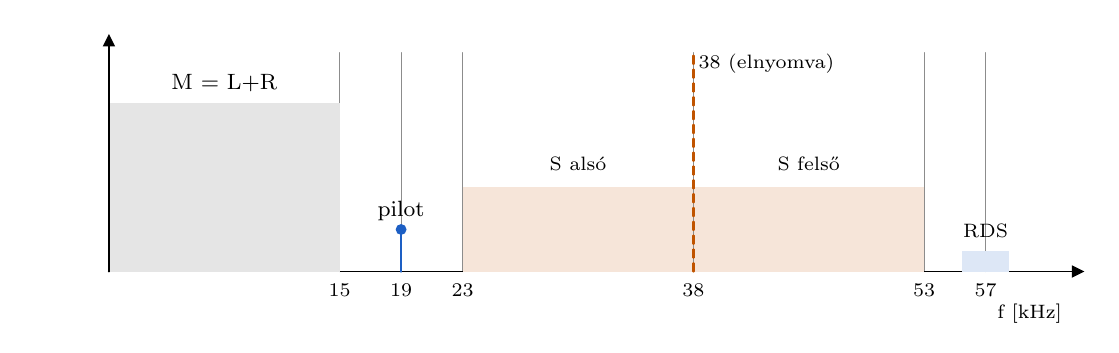
\begin{tikzpicture}[x=0.01985cm,y=-0.01985cm,line cap=round,line join=round]
\useasboundingbox (0,0) rectangle (680,190);
\path[draw=black!45,line width=0.35pt] (199.6,156) -- (199.6,16);
\path[draw=black!45,line width=0.35pt] (238.9,156) -- (238.9,16);
\path[draw=black!45,line width=0.35pt] (278.3,156) -- (278.3,16);
\path[draw=black!45,line width=0.35pt] (425.9,156) -- (425.9,16);
\path[draw=black!45,line width=0.35pt] (573.5,156) -- (573.5,16);
\path[draw=black!45,line width=0.35pt] (612.8,156) -- (612.8,16);
\path[draw=black,line width=0.7pt] (52,156) -- (670,156);
\path[fill=black,draw=none] (676,156) -- (668,152) -- (668,160) -- cycle;
\path[draw=black,line width=0.7pt] (52,156) -- (52,10);
\path[fill=black,draw=none] (52,4) -- (48,12) -- (56,12) -- cycle;
\node[anchor=base,inner sep=0pt,font=\scriptsize] at (199.6,172) {15};
\node[anchor=base,inner sep=0pt,font=\scriptsize] at (238.9,172) {19};
\node[anchor=base,inner sep=0pt,font=\scriptsize] at (278.3,172) {23};
\node[anchor=base,inner sep=0pt,font=\scriptsize] at (425.9,172) {38};
\node[anchor=base,inner sep=0pt,font=\scriptsize] at (573.5,172) {53};
\node[anchor=base,inner sep=0pt,font=\scriptsize] at (612.8,172) {57};
\node[anchor=base east,inner sep=0pt,font=\scriptsize] at (662,186) {f [kHz]};
\path[fill=black!10,draw=none] (52.5,156) -- (52.5,48.3) -- (199.6,48.3) -- (199.6,156) -- cycle;
\path[fill=cB!15,draw=none] (278.3,156) -- (278.3,102.2) -- (425.4,102.2) -- (425.4,156) -- cycle;
\path[fill=cB!15,draw=none] (426.4,156) -- (426.4,102.2) -- (573.5,102.2) -- (573.5,156) -- cycle;
\path[fill=cA!15,draw=none] (598,156) -- (598,143.1) -- (627.6,143.1) -- (627.6,156) -- cycle;
\path[draw=cB,line width=0.8pt,dash pattern=on 3pt off 2pt] (425.9,156) -- (425.9,16);
\node[anchor=base west,inner sep=0pt,font=\scriptsize] at (428.9,26) {38 (elnyomva)};
\path[draw=cA,line width=0.8pt,line width=0.99pt] (238.9,156) -- (238.9,129.1);
\path[fill=cA,draw=none] (238.9,129.1) circle[radius=0.069cm];
\node[anchor=base,inner sep=0pt,font=\footnotesize] at (238.9,121.1) {pilot};
\node[anchor=base,inner sep=0pt,font=\footnotesize] at (125.8,39.7) {M = L+R};
\node[anchor=base,inner sep=0pt,font=\scriptsize] at (352.1,91.4) {S alsó};
\node[anchor=base,inner sep=0pt,font=\scriptsize] at (499.7,91.4) {S felső};
\node[anchor=base,inner sep=0pt,font=\scriptsize] at (612.8,134.5) {RDS};
\end{tikzpicture}\end{center}
\begin{itemize}
\item $M$: 0,05\ldots{}15 kHz. Pilot: 19 kHz, kis vonal. $S$: 23\ldots{}53 kHz két oldalsávval, a 38 kHz-es segédvivő nincs benne. RDS: 57 kHz.
\end{itemize}

\textbf{b) 440 Hz-es fütty a bal mikrofonba}\par
\begin{center}\begin{tikzpicture}[x=0.01985cm,y=-0.01985cm,line cap=round,line join=round]
\useasboundingbox (0,0) rectangle (680,160);
\path[draw=black!45,line width=0.35pt] (58.4,126) -- (58.4,16);
\path[draw=black!45,line width=0.35pt] (328,126) -- (328,16);
\path[draw=black!45,line width=0.35pt] (597.5,126) -- (597.5,16);
\path[draw=black!45,line width=0.35pt] (610.3,126) -- (610.3,16);
\path[draw=black,line width=0.7pt] (52,126) -- (670,126);
\path[fill=black,draw=none] (676,126) -- (668,122) -- (668,130) -- cycle;
\path[draw=black,line width=0.7pt] (52,126) -- (52,10);
\path[fill=black,draw=none] (52,4) -- (48,12) -- (56,12) -- cycle;
\node[anchor=base,inner sep=0pt,font=\scriptsize] at (58.4,142) {0,44};
\node[anchor=base,inner sep=0pt,font=\scriptsize] at (328,142) {19};
\node[anchor=base,inner sep=0pt,font=\scriptsize] at (597.5,142) {37,56};
\node[anchor=base,inner sep=0pt,font=\scriptsize] at (610.3,142) {38,44};
\node[anchor=base east,inner sep=0pt,font=\scriptsize] at (662,156) {f [kHz]};
\path[draw=black,line width=0.8pt,line width=0.99pt] (58.4,126) -- (58.4,41.4);
\path[fill=black,draw=none] (58.4,41.4) circle[radius=0.069cm];
\path[draw=cA,line width=0.8pt,line width=0.99pt] (328,126) -- (328,104.8);
\path[fill=cA,draw=none] (328,104.8) circle[radius=0.069cm];
\path[draw=cB,line width=0.8pt,line width=0.99pt] (597.5,126) -- (597.5,83.7);
\path[fill=cB,draw=none] (597.5,83.7) circle[radius=0.069cm];
\path[draw=cB,line width=0.8pt,line width=0.99pt] (610.3,126) -- (610.3,83.7);
\path[fill=cB,draw=none] (610.3,83.7) circle[radius=0.069cm];
\end{tikzpicture}\end{center}
\begin{itemize}
\item Négy vonal: 0,44 kHz ($M$), 19 kHz (pilot), 37,56 és 38,44 kHz ($S$ két oldalsávja).
\end{itemize}
\end{rajz}
\begin{eredmeny}

\begin{center}\adjustbox{max width=\linewidth}{$\displaystyle \text{b) }0{,}44;\ 19;\ 37{,}56;\ 38{,}44\ \text{kHz}\qquad\text{c) }10;\ 19;\ 28;\ 48\ \text{kHz}\qquad\text{d) csak }19\ \text{kHz}$}\end{center}
\end{eredmeny}


% ------------------------------------------------------------------
\section{\texorpdfstring{9.6. feladat: Fütty a jobb mikrofonba: két feleletválasztós}{9.6. feladat: Fütty a jobb mikrofonba: két feleletválasztós}}\label{ai9_06}
\setcounter{lepes}{0}
\begin{feladat}{9.6. feladat}
a) 720 Hz: A) 18 280 Hz B) 19 720 Hz C) 19 kHz D) 38 720 Hz. b) 520 Hz: A) 38 520 Hz B) 520 Hz C) 38 kHz D) 19 kHz. Melyek a multiplex jel összetevői?

{\footnotesize\sffamily Forrás: ALL-IN 141\ldots{}142. oldal $\cdot$ aiD\_9\_11 (5.3.), aiD\_9\_13 (5.1.). Címkék: beugró, javítás}
\end{feladat}
\begin{keresunk}
\begin{itemize}
\item a multiplex jel összetevői
\end{itemize}
\end{keresunk}
\begin{jeloles}
\begin{jeltabla}
$M$ & az összegjel (L+R) & \\
$f$ & a fütty frekvenciája & \\
$S$ & a különbségi (L$-$R) jel & \\
\end{jeltabla}
\par\smallskip\textbf{Adott még:}
\begin{itemize}
\item egy hang a jobb csatornán
\end{itemize}
\end{jeloles}

\lepes{Az összetevők}
A jobb csatorna hangja $M$-ben $+f$, $S$-ben $-f$ előjellel szerepel, a frekvenciák ugyanazok, mint balra (A2). A 38 kHz-es segédvivő el van nyomva, a pilot mindig jelen van.

\begin{center}\adjustbox{max width=\linewidth}{$\displaystyle f,\quad38\pm f,\quad19\ \text{kHz}$}\end{center}
\jegyzet{definíció}{}

\lepes{a) 720 Hz}


\begin{center}\adjustbox{max width=\linewidth}{$\displaystyle 0{,}72;\ 19;\ 37{,}28;\ 38{,}72\ \text{kHz}$}\end{center}
\jegyzet{számérték}{C és D igaz}

\lepes{b) 520 Hz}


\begin{center}\adjustbox{max width=\linewidth}{$\displaystyle 0{,}52;\ 19;\ 37{,}48;\ 38{,}52\ \text{kHz}$}\end{center}
\jegyzet{számérték}{A, B és D igaz, C hamis (elnyomott)}
\begin{figyelem}[Javítás]
A gyűjtemény az a)-ra csak D-t (megjegyzéssel: „a C-t nem kéne bejelölni?”), a b)-re A, B-t ad. A pilot a multiplex jel része.
\end{figyelem}
\begin{eredmeny}

\begin{center}\adjustbox{max width=\linewidth}{$\displaystyle \text{a) C és D}\qquad\text{b) A, B és D}$}\end{center}
\end{eredmeny}


% ------------------------------------------------------------------
\section{\texorpdfstring{9.7. feladat: Ha az S komponens 6 dB-lel csillapodik}{9.7. feladat: Ha az S komponens 6 dB-lel csillapodik}}\label{ai9_07}
\setcounter{lepes}{0}
\begin{feladat}{9.7. feladat}
a) Az FM sztereó alapsávi spektruma. b) Miért halljuk mono vevőn mindkét csatornát? c) Mi történik, ha az amplitúdóhelyes $M$-hez képest $S$ 6 dB-lel csillapodik?

{\footnotesize\sffamily Forrás: ALL-IN 12., 57. oldal $\cdot$ ai2020\_06\_02\_Q2, ai2014\_12\_15\_5. Címkék: vizsga, javítás}
\end{feladat}
\begin{keresunk}
\begin{itemize}
\item a) spektrum
\item b) indoklás
\item c) a visszaállított $L'$ (a vevő bal kimenete), $R'$ (a vevő jobb kimenete)
\end{itemize}
\end{keresunk}
\begin{jeloles}
\begin{jeltabla}
$S$ & a különbségi (L$-$R) jel & \\
$M$ & az összegjel (L+R) & \\
\end{jeltabla}
\par\smallskip\textbf{Adott még:}
\begin{itemize}
\item $S$ (a különbségi (L$-$R) jel) az $M$-hez (az összegjel (L+R)) képest $-6$ dB, azaz feleakkora amplitúdójú
\end{itemize}
\end{jeloles}

\lepes{a), b)}
A multiplex jel: $M=L+R$ 15 kHz-ig, 19 kHz-es pilot, $S=L-R$ a 38 kHz-es elnyomott segédvivő két oldalán (23 és 53 kHz között), RDS 57 kHz-en. A mono vevő a 15 kHz-es aluláteresztő után csak $M=L+R$-et kapja, ebben mindkét csatorna benne van.

\lepes{c) A vevő visszaállítása}
Legyen $M=(L+R)/2$ és $S=(L-R)/2$, a vevő $L'=M+S$, $R'=M-S$-et képez. Ha $S$ fele akkora:

\begin{center}\adjustbox{max width=\linewidth}{$\displaystyle L'=\frac{L+R}{2}+\frac{L-R}{4}=0{,}75L+0{,}25R\qquad R'=0{,}25L+0{,}75R$}\end{center}
\jegyzet{behelyettesítés}{}

\begin{center}\adjustbox{max width=\linewidth}{$\displaystyle 20\lg\frac{0{,}75}{0{,}25}=20\lg3=9{,}5\ \text{dB}$}\end{center}
\jegyzet{számérték}{csatornaelválasztás}

\begin{rajz}
\textbf{Az FM sztereó alapsávi spektruma}\par
\begin{center}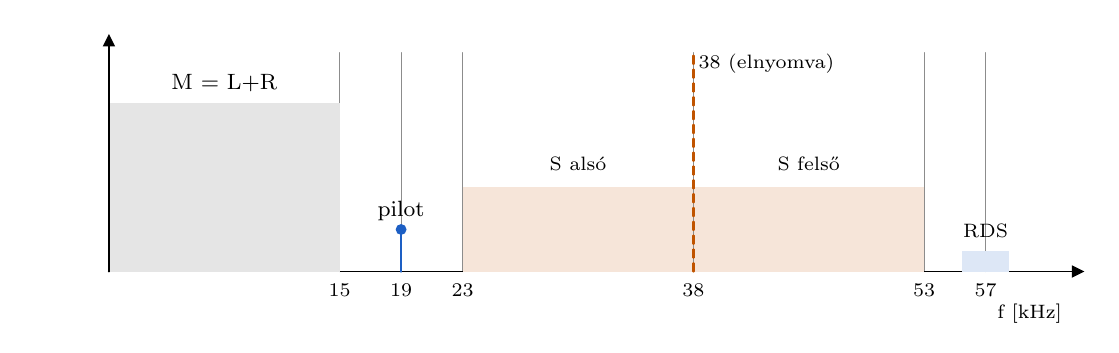
\begin{tikzpicture}[x=0.01985cm,y=-0.01985cm,line cap=round,line join=round]
\useasboundingbox (0,0) rectangle (680,190);
\path[draw=black!45,line width=0.35pt] (199.6,156) -- (199.6,16);
\path[draw=black!45,line width=0.35pt] (238.9,156) -- (238.9,16);
\path[draw=black!45,line width=0.35pt] (278.3,156) -- (278.3,16);
\path[draw=black!45,line width=0.35pt] (425.9,156) -- (425.9,16);
\path[draw=black!45,line width=0.35pt] (573.5,156) -- (573.5,16);
\path[draw=black!45,line width=0.35pt] (612.8,156) -- (612.8,16);
\path[draw=black,line width=0.7pt] (52,156) -- (670,156);
\path[fill=black,draw=none] (676,156) -- (668,152) -- (668,160) -- cycle;
\path[draw=black,line width=0.7pt] (52,156) -- (52,10);
\path[fill=black,draw=none] (52,4) -- (48,12) -- (56,12) -- cycle;
\node[anchor=base,inner sep=0pt,font=\scriptsize] at (199.6,172) {15};
\node[anchor=base,inner sep=0pt,font=\scriptsize] at (238.9,172) {19};
\node[anchor=base,inner sep=0pt,font=\scriptsize] at (278.3,172) {23};
\node[anchor=base,inner sep=0pt,font=\scriptsize] at (425.9,172) {38};
\node[anchor=base,inner sep=0pt,font=\scriptsize] at (573.5,172) {53};
\node[anchor=base,inner sep=0pt,font=\scriptsize] at (612.8,172) {57};
\node[anchor=base east,inner sep=0pt,font=\scriptsize] at (662,186) {f [kHz]};
\path[fill=black!10,draw=none] (52.5,156) -- (52.5,48.3) -- (199.6,48.3) -- (199.6,156) -- cycle;
\path[fill=cB!15,draw=none] (278.3,156) -- (278.3,102.2) -- (425.4,102.2) -- (425.4,156) -- cycle;
\path[fill=cB!15,draw=none] (426.4,156) -- (426.4,102.2) -- (573.5,102.2) -- (573.5,156) -- cycle;
\path[fill=cA!15,draw=none] (598,156) -- (598,143.1) -- (627.6,143.1) -- (627.6,156) -- cycle;
\path[draw=cB,line width=0.8pt,dash pattern=on 3pt off 2pt] (425.9,156) -- (425.9,16);
\node[anchor=base west,inner sep=0pt,font=\scriptsize] at (428.9,26) {38 (elnyomva)};
\path[draw=cA,line width=0.8pt,line width=0.99pt] (238.9,156) -- (238.9,129.1);
\path[fill=cA,draw=none] (238.9,129.1) circle[radius=0.069cm];
\node[anchor=base,inner sep=0pt,font=\footnotesize] at (238.9,121.1) {pilot};
\node[anchor=base,inner sep=0pt,font=\footnotesize] at (125.8,39.7) {M = L+R};
\node[anchor=base,inner sep=0pt,font=\scriptsize] at (352.1,91.4) {S alsó};
\node[anchor=base,inner sep=0pt,font=\scriptsize] at (499.7,91.4) {S felső};
\node[anchor=base,inner sep=0pt,font=\scriptsize] at (612.8,134.5) {RDS};
\end{tikzpicture}\end{center}
\begin{itemize}
\item $M$: 0,05\ldots{}15 kHz. Pilot: 19 kHz, kis vonal. $S$: 23\ldots{}53 kHz két oldalsávval, a 38 kHz-es segédvivő nincs benne. RDS: 57 kHz.
\end{itemize}
\end{rajz}
\begin{figyelem}[Javítás]
A Moodle-válasz (a zaj „jobban beleszámít”) 0 pontot kapott, az ALL-IN 2014-es változatában „passz”.
\end{figyelem}
\begin{eredmeny}

\begin{center}\adjustbox{max width=\linewidth}{$\displaystyle \text{c) áthallás: a bal csatornában a jobb is szól, csak 9,5 dB-lel halkabban, a sztereó kép összeszűkül}$}\end{center}
\end{eredmeny}


% ------------------------------------------------------------------
\section{\texorpdfstring{9.8. feladat: DVB-C 256-QAM-mel, $\alpha$ = 1/3}{9.8. feladat: DVB-C 256-QAM-mel, α = 1/3}}\label{ai9_08}
\setcounter{lepes}{0}
\begin{feladat}{9.8. feladat}
8 MHz-es raszter, 33,33\%-os emelt koszinusz, 256-QAM (RS nélkül). a) Szimbólum- és bitsebesség? b) Hány 1,5 Mbit/s-os csatorna fér el, mi a 6 Mbit/s-os kódolás előnye és hátránya? c) Mi az 1024-QAM előnye és hátránya?

{\footnotesize\sffamily Forrás: ALL-IN 32\ldots{}34., 75\ldots{}76., 127. oldal $\cdot$ ai2015\_12\_16\_4, ai2014\_01\_07\_9, aiD\_7\_11 (és 5-ösöm 6. oldal). Címkék: vizsga}
\end{feladat}
\begin{keresunk}
\begin{itemize}
\item a) $1/T$, $v$ (bitsebesség)
\item b) csatornaszám
\item c) 1024-QAM
\end{itemize}
\end{keresunk}
\begin{jeloles}
\begin{jeltabla}
$\ca{B}$ & a csatorna sávszélessége & $8$\,MHz\\
$\alpha$ & lekerekítési tényező & \\
$\cb{M}$ & az összegjel (L+R) & $256$\\
$v$ & bitsebesség & \emph{keresett}\\
\end{jeltabla}
\end{jeloles}

\lepes{a) Szimbólumsebesség}
Vivőfrekvenciás emelt koszinusz: $(1+\alpha)/T\le {\ca{B}}$.

\begin{center}\adjustbox{max width=\linewidth}{$\displaystyle \frac43\cdot\frac1T\le8\ \text{MHz}\ \Rightarrow\ \frac1T=6\ \text{MBd}$}\end{center}
\jegyzet{tétel}{}

\lepes{a), b) Bitsebesség, csatornák}
$\log_2256=8$ bit/szimbólum.

\begin{center}\adjustbox{max width=\linewidth}{$\displaystyle 6\cdot8=48\ \text{Mbit/s}\qquad\frac{48}{1{,}5}=32\ \text{csatorna}$}\end{center}
\jegyzet{számérték}{}

\begin{center}\adjustbox{max width=\linewidth}{$\displaystyle \frac{48}{6}=8\ \text{csatorna}$}\end{center}
\jegyzet{számérték}{6 Mbit/s-mal: jobb kép (HD), de kevesebb műsor}

\lepes{c) 1024-QAM}
10 bit/szimbólum: $6\cdot10=60$ Mbit/s (40 csatorna). A pontok sűrűbbek: kisebb zaj- és fázistűrés (kb. 1,8\textdegree{}), nagyobb jel-zaj viszony kell.
\begin{eredmeny}

\begin{center}\adjustbox{max width=\linewidth}{$\displaystyle \text{a) }6\ \text{MBd},\ 48\ \text{Mbit/s}\qquad\text{b) }32\ \text{csatorna (6 Mbit/s-mal 8)}\qquad\text{c) 60 Mbit/s, de kisebb zajtűrés}$}\end{center}
\end{eredmeny}


% ------------------------------------------------------------------
\section{\texorpdfstring{9.9. feladat: DVB-C 64-QAM-mel, $\alpha$ = 15\%, RS(204,188)}{9.9. feladat: DVB-C 64-QAM-mel, α = 15, RS(204,188)}}\label{ai9_09}
\setcounter{lepes}{0}
\begin{feladat}{9.9. feladat}
Hány 1,5 Mbit/s-os csatorna fér el egy 8 MHz-es raszterben 64-QAM-mel, 15\%-os lekerekítéssel és RS(204,188) kóddal?

{\footnotesize\sffamily Forrás: ALL-IN 58\ldots{}60. oldal $\cdot$ ai2014\_12\_15\_7. Címkék: vizsga, javítás}
\end{feladat}
\begin{keresunk}
\begin{itemize}
\item a csatornák száma
\end{itemize}
\end{keresunk}
\begin{jeloles}
\begin{jeltabla}
$\ca{B}$ & a csatorna sávszélessége & $8$\,MHz\\
$\alpha$ & lekerekítési tényező & \\
$\cb{M}$ & az összegjel (L+R) & $64$\\
$T$ & a szimbólumidő & \\
\end{jeltabla}
\par\smallskip\textbf{Adott még:}
\begin{itemize}
\item RS(204,188): 204 bájtból 188 hasznos, kódarány $188/204$
\end{itemize}
\end{jeloles}

\lepes{Szimbólumsebesség}
$(1+\alpha)/T\le {\ca{B}}$, ez felső korlát, felfelé nem kerekíthetünk.

\begin{center}\adjustbox{max width=\linewidth}{$\displaystyle \frac1T=\frac{8}{1{,}15}=6{,}957\ \text{MBd}$}\end{center}
\jegyzet{tétel}{}

\lepes{Nettó bitsebesség és csatornák}


\begin{center}\adjustbox{max width=\linewidth}{$\displaystyle 6{,}957\cdot6\cdot\frac{188}{204}=41{,}74\cdot0{,}922=38{,}47\ \text{Mbit/s}$}\end{center}
\jegyzet{számérték}{}

\begin{center}\adjustbox{max width=\linewidth}{$\displaystyle \frac{38{,}47}{1{,}5}=25{,}6\ \Rightarrow\ 25\ \text{csatorna}$}\end{center}
\jegyzet{számérték}{csak egész csatorna fér el}
\begin{figyelem}[Javítás]
A gyűjtemény 7 MBd-ra kerekít felfelé (ehhez már 8,05 MHz kellene). A csatornaszám véletlenül ugyanaz.
\end{figyelem}
\begin{eredmeny}

\begin{center}\adjustbox{max width=\linewidth}{$\displaystyle 25\ \text{csatorna}$}\end{center}
\end{eredmeny}


% ------------------------------------------------------------------
\section{\texorpdfstring{9.10. feladat: Fogalmak: QAM, AM-VSB, OFDM, egyfrekvenciás hálózat}{9.10. feladat: Fogalmak: QAM, AM-VSB, OFDM, egyfrekvenciás hálózat}}\label{ai9_10}
\setcounter{lepes}{0}
\begin{feladat}{9.10. feladat}
Miért QAM és AM-VSB a műsorszórásban? Ismertesse az analóg földi és műholdas, a digitális földi TV és az egyfrekvenciás hálózat jellemzőit! Miért lehet OFDM-mel SFN-t építeni?

{\footnotesize\sffamily Forrás: ALL-IN 137., 140., 145. oldal $\cdot$ aiD\_9\_3, aiD\_9\_6, aiD\_10\_1 (és 5-ösöm 24. oldal). Címkék: beugró}
\end{feladat}
\begin{keresunk}
\begin{itemize}
\item indokolt válaszok
\end{itemize}
\end{keresunk}
\begin{jeloles}
\par\smallskip\textbf{Adott még:}
\begin{itemize}
\item fogalmi kérdések
\end{itemize}
\end{jeloles}

\lepes{QAM}
Két, egymásra merőleges (koszinusz és szinusz) vivővel két független jelet (a két színkülönbségi jelet, illetve két adatcsatornát) visz ugyanabban a sávban, egymás zavarása nélkül.

\lepes{AM-VSB}
A képjel széles (kb. 5 MHz) és egyenszintet is tartalmaz. AM-DSB-vel 10 MHz kellene: pazarló. SSB-hez a vivő közvetlen közelében kellene éles szűrő, ez DC-tartalmú jelnél nem megy. A csonka oldalsáv majdnem felezi a sávot, és a jel burkolóval demodulálható.

\lepes{A rendszerek}
Analóg földi TV: kép AM-VSB, szín QAM, hang FM, 7 vagy 8 MHz-es csatorna. Analóg műholdas: FM, 10,7 és 12,75 GHz között, kb. 27 MHz. DVB-T: OFDM (2k vagy 8k vivő), QPSK, 16-QAM vagy 64-QAM, konvolúciós kód és RS(204,188), 7,61 MHz.

\lepes{SFN és OFDM}
Egyfrekvenciás hálózat (SFN): több adó szinkronban, ugyanazon a frekvencián sugározza ugyanazt. A vevőben a többi adó jele késleltetett visszhangként jelenik meg. Az OFDM szimbólumai hosszúak, és védőintervallum előzi meg őket: ha a késés ezen belül van, a visszhang nem okoz ISI-t, sőt a teljesítménye hasznosul.
\begin{eredmeny}

\begin{center}\adjustbox{max width=\linewidth}{$\displaystyle \text{QAM: két jel egy sávban}\quad\text{VSB: fél sáv, burkolós vétel}\quad\text{SFN: a védőintervallumon belüli visszhang hasznos}$}\end{center}
\end{eredmeny}


% ------------------------------------------------------------------
\section{\texorpdfstring{9.11. feladat: PDH és E1: négy állítás}{9.11. feladat: PDH és E1: négy állítás}}\label{ai9_11}
\setcounter{lepes}{0}
\begin{feladat}{9.11. feladat}
A) Pleziokron Digitális Hierarchia. B) E1 szinten 32 időrésben beszéd. C) Egy időrés 3,9 \textmu{}s ($\pm$1\%). D) Csatornánként a jelzés 2 kbit/s.

{\footnotesize\sffamily Forrás: ALL-IN 142. oldal $\cdot$ aiD\_9\_14 (5.2.). Címkék: beugró}
\end{feladat}
\begin{keresunk}
\begin{itemize}
\item melyik állítás igaz
\end{itemize}
\end{keresunk}
\begin{jeloles}
\par\smallskip\textbf{Adott még:}
\begin{itemize}
\item E1: 2,048 Mbit/s, 125 \textmu{}s-os keret (8 kHz-es mintavétel), 32 időrés, időrésenként 8 bit
\item TS0: keretszinkron, TS16: jelzés, a többi 30 beszéd
\end{itemize}
\end{jeloles}

\lepes{A), B)}
A PDH a Plesiochronous Digital Hierarchy rövidítése: A igaz. A 32 időrésből csak 30 beszéd: B hamis.

\lepes{C) Időrés hossza}


\begin{center}\adjustbox{max width=\linewidth}{$\displaystyle \frac{125\ \mu\text{s}}{32}=3{,}906\ \mu\text{s}$}\end{center}
\jegyzet{számérték}{C igaz}

\lepes{D) Jelzés csatornánként}
A TS16 16 keretből álló multikeretben váltakozva viszi a 30 csatorna jelzését: csatornánként 4 bitet 16 keretenként.

\begin{center}\adjustbox{max width=\linewidth}{$\displaystyle \frac{4\ \text{bit}}{16\cdot125\ \mu\text{s}}=\frac{4}{2\ \text{ms}}=2\ \text{kbit/s}$}\end{center}
\jegyzet{számérték}{D igaz}
\begin{eredmeny}

\begin{center}\adjustbox{max width=\linewidth}{$\displaystyle \text{A, C, D igaz, B hamis}$}\end{center}
\end{eredmeny}
\begin{tipp}[Ellenőrzés]
\begin{itemize}
\item A gyűjtemény A, D-t ad. A C számszerűen igaz, a kérdező szándéka \texttt{[ELLENŐRIZENDŐ]}.
\end{itemize}
\end{tipp}

% Generálva: html/build_tex.js (ai10.js). Kézzel ne szerkeszd, a forrás a html/data mappa.
\setcounter{chapter}{9}
\chapter{\texorpdfstring{Cellás mobilhálózat (GSM)}{Cellás mobilhálózat (GSM)}}\label{f10}
Kapacitásbecslés klaszterekkel és frekvencia-újrafelhasználással, valamint a roamingos „melyik HLR, melyik SMSC” kérdések. Ezekhez néhány szabályt kell biztosan tudni, a válaszoknál mindig ott van, melyikből jön.

\section{Alapok, egyszerűen}
\subsection{\texorpdfstring{A1. Kapacitás: vivők, időrések, klaszter}{A1. Kapacitás: vivők, időrések, klaszter}}\label{a10-kapacitas}
GSM 900: irányonként 25 MHz, 200 kHz-es vivők (124 db), vivőnként 8 időrés (TDMA). Egy \textbf{klaszter} $N$ cellából áll ($N$ = FRF, frekvencia-újrafelhasználási tényező): a vivőket szétosztják köztük, így egy klaszter minden vivőt pontosan egyszer használ. $C$ vivővel egy cellában $\approx C/N$ vivő, egyszerre $8C/N$ beszélgetés (a jelzési időréseket elhanyagolva), klaszterenként $8C$.

Nagy $N$: az azonos frekvenciájú cellák távolabb vannak, kisebb az interferencia, de kevesebb vivő jut egy cellára.

\subsection{\texorpdfstring{A2. Elemek és szabályok}{A2. Elemek és szabályok}}\label{a10-roaming}
MS: készülék. BTS: bázisállomás (rádió). BSC: bázisállomás-vezérlő. MSC: kapcsolóközpont. GMSC: átjáró MSC, a kívülről jövő hívást fogadja és a HLR-t kérdezi. HLR: honi adatbázis (hol van az előfizető). VLR: látogatói adatbázis. AuC: hitelesítés. EIR: készülék-nyilvántartás. SMSC: SMS-központ. Az index ($\alpha$, $\beta$) a szolgáltatót jelöli.

\begin{enumerate}
\item \textbf{Hívásnál a hívott honi HLR-jét} kérdezik le, a hívott honi hálózatának GMSC-je értesül először.
\item \textbf{Az SMS-t a küldő honi SMSC-je} fogadja és kézbesíti.
\item \textbf{Beszélgetés közbeni mozgásról} (hívásátadás) csak a kiszolgáló hálózat BTS-e, BSC-je és MSC-je tud. Hívás nélküli mozgásnál helyzetfrissítés van: a VLR, és VLR-váltáskor a honi HLR is értesül.
\item Egy eseményről (hívásindítás, bontás) először a kezdeményező saját BTS-e tud.
\end{enumerate}

Hitelesítés: AuC (Ki, A3 $\to$ SRES, A8 $\to$ Kc), rejtjelezés A5-tel. Készülékellenőrzés: a kiszolgáló hálózat EIR-je (fehér, fekete, szürke = megfigyelt lista). FNR: számhordozhatóság.

% ------------------------------------------------------------------
\section{\texorpdfstring{10.1. feladat: N = 7 klaszter, 70 csatorna (Moodle 2020)}{10.1. feladat: N = 7 klaszter, 70 csatorna (Moodle 2020)}}\label{ai10_01}
\setcounter{lepes}{0}
\begin{feladat}{10.1. feladat}
a) Rajzoljon N = 7-es klasztert két szomszédjával. b) 70 FDM-csatornával hány aktív előfizető lehet a klaszterben? c) Mi az FRF szerepe, mi a nagy N előnye és hátránya?

{\footnotesize\sffamily Forrás: ALL-IN 6. oldal $\cdot$ ai2020\_05\_26\_Q6. Címkék: vizsga}
\end{feladat}
\begin{keresunk}
\begin{itemize}
\item a) rajz
\item b) egyszerre aktív előfizetők a klaszterben
\item c) indoklás
\end{itemize}
\end{keresunk}
\begin{jeloles}
\begin{jeltabla}
$\ca{N}$ & a klaszter cellaszáma (FRF) & $7$\\
\end{jeltabla}
\par\smallskip\textbf{Adott még:}
\begin{itemize}
\item 70 FDM-csatorna (vivő), vivőnként 8 időrés
\end{itemize}
\end{jeloles}

\lepes{a) Rajz}
Egy középső hatszög és körülötte hat: ez egy klaszter, 1-től 7-ig számozva. Két szomszéd klaszter ugyanígy, eltolva, úgy, hogy az azonos számú cellák egymástól a lehető legmesszebb kerüljenek.

\lepes{b) Aktív előfizetők}
A klaszter minden vivőt egyszer használ fel (A1), minden vivőn 8 időrés.

\begin{center}\adjustbox{max width=\linewidth}{$\displaystyle 70\cdot8=560$}\end{center}
\jegyzet{számérték}{klaszterenként}

\lepes{c) Az FRF szerepe}
Megadja, hány cella után lehet ugyanazt a vivőt újra használni. Nagy N: az azonos vivőt használó cellák távolabb, kisebb az azonos csatornás interferencia. Hátrány: cellánként kevesebb vivő jut (pl. 120 vivő, N = 12: csak 10 vivő, 80 beszélgetés). Tipikus értékek: 3, 7, 12.

\begin{rajz}
\textbf{N = 7-es klaszter két szomszédjával}\par
\begin{center}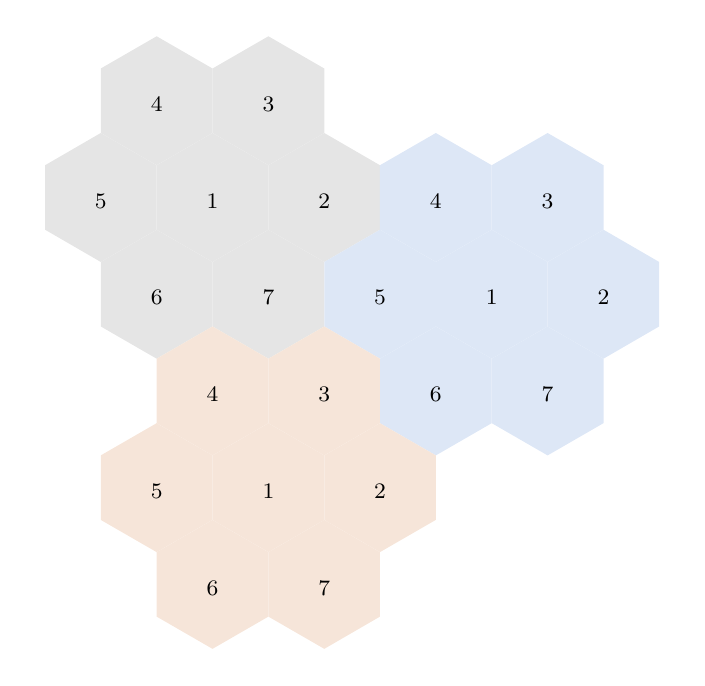
\begin{tikzpicture}[x=0.02730cm,y=-0.02730cm,line cap=round,line join=round]
\useasboundingbox (-86,-79) rectangle (216,214);
\path[fill=black!10,draw=none] (26,-15) -- (26,15) -- (0,30) -- (-26,15) -- (-26,-15) -- (0,-30) -- cycle;
\node[anchor=base,inner sep=0pt,font=\footnotesize] at (0,5) {1};
\path[fill=black!10,draw=none] (77.9,-15) -- (77.9,15) -- (52,30) -- (26,15) -- (26,-15) -- (52,-30) -- cycle;
\node[anchor=base,inner sep=0pt,font=\footnotesize] at (52,5) {2};
\path[fill=black!10,draw=none] (52,-60) -- (52,-30) -- (26,-15) -- (0,-30) -- (0,-60) -- (26,-75) -- cycle;
\node[anchor=base,inner sep=0pt,font=\footnotesize] at (26,-40) {3};
\path[fill=black!10,draw=none] (0,-60) -- (0,-30) -- (-26,-15) -- (-52,-30) -- (-52,-60) -- (-26,-75) -- cycle;
\node[anchor=base,inner sep=0pt,font=\footnotesize] at (-26,-40) {4};
\path[fill=black!10,draw=none] (-26,-15) -- (-26,15) -- (-52,30) -- (-77.9,15) -- (-77.9,-15) -- (-52,-30) -- cycle;
\node[anchor=base,inner sep=0pt,font=\footnotesize] at (-52,5) {5};
\path[fill=black!10,draw=none] (0,30) -- (0,60) -- (-26,75) -- (-52,60) -- (-52,30) -- (-26,15) -- cycle;
\node[anchor=base,inner sep=0pt,font=\footnotesize] at (-26,50) {6};
\path[fill=black!10,draw=none] (52,30) -- (52,60) -- (26,75) -- (0,60) -- (0,30) -- (26,15) -- cycle;
\node[anchor=base,inner sep=0pt,font=\footnotesize] at (26,50) {7};
\path[fill=cA!15,draw=none] (155.9,30) -- (155.9,60) -- (129.9,75) -- (103.9,60) -- (103.9,30) -- (129.9,15) -- cycle;
\node[anchor=base,inner sep=0pt,font=\footnotesize] at (129.9,50) {1};
\path[fill=cA!15,draw=none] (207.8,30) -- (207.8,60) -- (181.9,75) -- (155.9,60) -- (155.9,30) -- (181.9,15) -- cycle;
\node[anchor=base,inner sep=0pt,font=\footnotesize] at (181.9,50) {2};
\path[fill=cA!15,draw=none] (181.9,-15) -- (181.9,15) -- (155.9,30) -- (129.9,15) -- (129.9,-15) -- (155.9,-30) -- cycle;
\node[anchor=base,inner sep=0pt,font=\footnotesize] at (155.9,5) {3};
\path[fill=cA!15,draw=none] (129.9,-15) -- (129.9,15) -- (103.9,30) -- (77.9,15) -- (77.9,-15) -- (103.9,-30) -- cycle;
\node[anchor=base,inner sep=0pt,font=\footnotesize] at (103.9,5) {4};
\path[fill=cA!15,draw=none] (103.9,30) -- (103.9,60) -- (77.9,75) -- (52,60) -- (52,30) -- (77.9,15) -- cycle;
\node[anchor=base,inner sep=0pt,font=\footnotesize] at (77.9,50) {5};
\path[fill=cA!15,draw=none] (129.9,75) -- (129.9,105) -- (103.9,120) -- (77.9,105) -- (77.9,75) -- (103.9,60) -- cycle;
\node[anchor=base,inner sep=0pt,font=\footnotesize] at (103.9,95) {6};
\path[fill=cA!15,draw=none] (181.9,75) -- (181.9,105) -- (155.9,120) -- (129.9,105) -- (129.9,75) -- (155.9,60) -- cycle;
\node[anchor=base,inner sep=0pt,font=\footnotesize] at (155.9,95) {7};
\path[fill=cB!15,draw=none] (52,120) -- (52,150) -- (26,165) -- (0,150) -- (0,120) -- (26,105) -- cycle;
\node[anchor=base,inner sep=0pt,font=\footnotesize] at (26,140) {1};
\path[fill=cB!15,draw=none] (103.9,120) -- (103.9,150) -- (77.9,165) -- (52,150) -- (52,120) -- (77.9,105) -- cycle;
\node[anchor=base,inner sep=0pt,font=\footnotesize] at (77.9,140) {2};
\path[fill=cB!15,draw=none] (77.9,75) -- (77.9,105) -- (52,120) -- (26,105) -- (26,75) -- (52,60) -- cycle;
\node[anchor=base,inner sep=0pt,font=\footnotesize] at (52,95) {3};
\path[fill=cB!15,draw=none] (26,75) -- (26,105) -- (0,120) -- (-26,105) -- (-26,75) -- (0,60) -- cycle;
\node[anchor=base,inner sep=0pt,font=\footnotesize] at (0,95) {4};
\path[fill=cB!15,draw=none] (0,120) -- (0,150) -- (-26,165) -- (-52,150) -- (-52,120) -- (-26,105) -- cycle;
\node[anchor=base,inner sep=0pt,font=\footnotesize] at (-26,140) {5};
\path[fill=cB!15,draw=none] (26,165) -- (26,195) -- (0,210) -- (-26,195) -- (-26,165) -- (0,150) -- cycle;
\node[anchor=base,inner sep=0pt,font=\footnotesize] at (0,185) {6};
\path[fill=cB!15,draw=none] (77.9,165) -- (77.9,195) -- (52,210) -- (26,195) -- (26,165) -- (52,150) -- cycle;
\node[anchor=base,inner sep=0pt,font=\footnotesize] at (52,185) {7};
\end{tikzpicture}\end{center}
\begin{itemize}
\item Egy klaszter: egy középső hatszög és a hat szomszédja, 1-től 7-ig számozva. A szomszéd klasztereket úgy told el (két cella egy irányba, egy cella 60\textdegree{}-kal elfordulva), hogy az azonos számú cellák egymástól a lehető legmesszebb legyenek.
\end{itemize}
\end{rajz}
\begin{eredmeny}

\begin{center}\adjustbox{max width=\linewidth}{$\displaystyle \text{b) }560\ \text{aktív előfizető}$}\end{center}
\end{eredmeny}


% ------------------------------------------------------------------
\section{\texorpdfstring{10.2. feladat: Győr: klaszter, egyidejű hívások, VAD, FNR}{10.2. feladat: Győr: klaszter, egyidejű hívások, VAD, FNR}}\label{ai10_02}
\setcounter{lepes}{0}
\begin{feladat}{10.2. feladat}
Győr 170 km\textsuperscript{2}, FRF = 12, kb. 85 GSM-cella. a) Mekkora egy klaszter? b) Hányan telefonálhatnak egyszerre? c) Egy szolgáltató 40 FDM-csatornát használ: hányan egy cellában nála? d) Mi a VAD előnye? e) Mire az FNR és az AuC?

{\footnotesize\sffamily Forrás: ALL-IN 25\ldots{}27., 145. oldal $\cdot$ ai2016\_06\_07\_3. Címkék: vizsga}
\end{feladat}
\begin{keresunk}
\begin{itemize}
\item a) a klaszter területe
\item b) egyidejű hívások
\item c) egy cellában egy szolgáltatónál
\item d), e) fogalmak
\end{itemize}
\end{keresunk}
\begin{jeloles}
\begin{jeltabla}
$T_\text{cella}$ & egy cella területe & \\
$T_\text{klaszter}$ & egy klaszter területe & \\
\end{jeltabla}
\par\smallskip\textbf{Adott még:}
\begin{itemize}
\item 124 vivő, vivőnként 8 időrés
\item c) egy szolgáltató 40 vivőt használ
\end{itemize}
\end{jeloles}

\lepes{a) Klaszter}
Először egy cella területe, majd 12 cella.

\begin{center}\adjustbox{max width=\linewidth}{$\displaystyle T_\text{cella}=\frac{170}{85}=2\ \text{km}^2\qquad T_\text{klaszter}=12\cdot2=24\ \text{km}^2$}\end{center}
\jegyzet{számérték}{}

\lepes{b) Egyidejű hívások}
Egy cellára $124\cdot8/12=82{,}7$ beszélgetés jut (A1).

\begin{center}\adjustbox{max width=\linewidth}{$\displaystyle 85\cdot\frac{124\cdot8}{12}=85\cdot82{,}7\approx7000$}\end{center}
\jegyzet{számérték}{ugyanez: $85/12\approx7$ klaszter $\cdot992$}

\lepes{c) Egy szolgáltató}
A 40 vivő oszlik meg a klaszter 12 cellája között.

\begin{center}\adjustbox{max width=\linewidth}{$\displaystyle \frac{40}{12}=3{,}33\ \text{vivő}\ \Rightarrow\ 3\cdot8=24\ \text{(néhol }4\cdot8=32)$}\end{center}
\jegyzet{számérték}{átlagosan kb. 26}

\lepes{d), e) Fogalmak}
VAD + DTX: beszédszünetben nincs adás, kevesebb fogyasztás és interferencia, a vevő komfortzajt generál. FNR: számhordozhatósági adatbázis. AuC: a SIM titkos kulcsának (Ki) tárolása, a hitelesítési adatok (RAND, SRES, Kc) előállítása.
\begin{eredmeny}

\begin{center}\adjustbox{max width=\linewidth}{$\displaystyle \text{a) }24\ \text{km}^2\qquad\text{b) }\approx7000\qquad\text{c) }\approx24\ldots32$}\end{center}
\end{eredmeny}
\begin{tipp}[Ellenőrzés]
\begin{itemize}
\item c) A gyűjteményben „passz”, a saját megoldás feltevése, hogy a 40 vivő a klaszterre vonatkozik \texttt{[ELLENŐRIZENDŐ]}.
\end{itemize}
\end{tipp}


% ------------------------------------------------------------------
\section{\texorpdfstring{10.3. feladat: Két roamingoló előfizető hívása és SMS-e}{10.3. feladat: Két roamingoló előfizető hívása és SMS-e}}\label{ai10_03}
\setcounter{lepes}{0}
\begin{feladat}{10.3. feladat}
MS-A az $\alpha$, MS-B a $\beta$ előfizetője, egymás hálózatában barangolnak. MS-A felhívja MS-B-t. a) Melyik HLR-t kérdezik? b) Melyik GMSC értesül előbb? c) Ki tud MS-A beszélgetés közbeni mozgásáról? d) Bontás után MS-B SMS-t küld MS-A-nak, melyik SMSC kézbesíti?

{\footnotesize\sffamily Forrás: ALL-IN 21\ldots{}22., 41. oldal $\cdot$ ai2016\_01\_05\_7, ai2016\_01\_05\_7b (és 5-ösöm 27. oldal). Címkék: vizsga, javítás}
\end{feladat}
\begin{keresunk}
\begin{itemize}
\item a) HLR
\item b) GMSC
\item c) a mozgásról tudó elemek
\item d) SMSC
\end{itemize}
\end{keresunk}
\begin{jeloles}
\begin{jeltabla}
$\beta$ & a másik szolgáltató ($\beta$) hálózata, alsó indexben: a $\beta$ hálózat eleme & \\
$\alpha$ & az egyik szolgáltató ($\alpha$) hálózata, alsó indexben: az $\alpha$ hálózat eleme & \\
\end{jeltabla}
\par\smallskip\textbf{Adott még:}
\begin{itemize}
\item MS-A: $\alpha$-előfizető, $\beta$-ban van
\item MS-B: $\beta$-előfizető, $\alpha$-ban van
\end{itemize}
\end{jeloles}

\lepes{A hívás útja}
MS-A $\beta$-ban hív: BTS$_\beta$ $\to$ BSC$_\beta$ $\to$ MSC$_\beta$. A hívott szám $\beta$-beli, ezért a GMSC$_\beta$ fogadja, megkérdezi a HLR$_\beta$-t, amely tudja, hogy MS-B a VLR$_\alpha$ területén van. A hívás innen az $\alpha$ hálózatba megy MS-B-hez.

\lepes{a), b)}
1. szabály: a hívott (MS-B, $\beta$-előfizető) honi HLR-je, és a honi hálózatának GMSC-je.

\begin{center}\adjustbox{max width=\linewidth}{$\displaystyle \text{HLR}_\beta,\ \text{GMSC}_\beta$}\end{center}
\jegyzet{definíció}{}

\lepes{c) Mozgás beszélgetés közben}
3. szabály: hívásátadás MS-A kiszolgáló hálózatában ($\beta$).

\begin{center}\adjustbox{max width=\linewidth}{$\displaystyle \text{BTS}_\beta,\ \text{BSC}_\beta,\ \text{MSC}_\beta$}\end{center}
\jegyzet{definíció}{}

\lepes{d) SMS}
2. szabály: a küldő (MS-B, $\beta$-előfizető) honi SMSC-je.

\begin{center}\adjustbox{max width=\linewidth}{$\displaystyle \text{SMSC}_\beta$}\end{center}
\jegyzet{definíció}{}
\begin{figyelem}[Javítás]
A c) részre a gyűjtemény a HLR$_\alpha$-t és a VLR$_\beta$-t is felsorolja. Hívás közben nincs helyzetfrissítés, ezek csak hívás nélküli mozgásnál értesülnek \texttt{[ELLENŐRIZENDŐ]}.
\end{figyelem}
\begin{eredmeny}

\begin{center}\adjustbox{max width=\linewidth}{$\displaystyle \text{a) HLR}_\beta\quad\text{b) GMSC}_\beta\quad\text{c) BTS}_\beta,\ \text{BSC}_\beta,\ \text{MSC}_\beta\quad\text{d) SMSC}_\beta$}\end{center}
\end{eredmeny}


% ------------------------------------------------------------------
\section{\texorpdfstring{10.4. feladat: Két $\alpha$-előfizető, az egyik $\beta$-ban (Moodle 2020)}{10.4. feladat: Két α-előfizető, az egyik β-ban (Moodle 2020)}}\label{ai10_04}
\setcounter{lepes}{0}
\begin{feladat}{10.4. feladat}
MS-A1 és MS-A2 is $\alpha$-előfizető, MS-A2 a $\beta$ hálózatban barangol. MS-A1 hívja MS-A2-t. a) Melyik eszközhöz érkezik először információ a hívásindításról? b) Melyik HLR-t kérdezik? c) Mely eszközök tudnak MS-A2 $\beta$-beli mozgásáról? d) Melyik eszközzel azonosítják MS-A1 SIM-jét?

{\footnotesize\sffamily Forrás: ALL-IN 8. oldal $\cdot$ ai2020\_05\_26\_Q8 (és 5-ösöm 28. oldal). Címkék: vizsga}
\end{feladat}
\begin{keresunk}
\begin{itemize}
\item a) az első eszköz
\item b) HLR
\item c) a mozgásról tudó elemek
\item d) a SIM azonosítása
\end{itemize}
\end{keresunk}
\begin{jeloles}
\begin{jeltabla}
$\alpha$ & az egyik szolgáltató ($\alpha$) hálózata, alsó indexben: az $\alpha$ hálózat eleme & \\
$\beta$ & a másik szolgáltató ($\beta$) hálózata, alsó indexben: a $\beta$ hálózat eleme & \\
\end{jeltabla}
\par\smallskip\textbf{Adott még:}
\begin{itemize}
\item MS-A1: $\alpha$-előfizető, $\alpha$-ban
\item MS-A2: $\alpha$-előfizető, $\beta$-ban
\end{itemize}
\end{jeloles}

\lepes{a) Hívásindítás}
4. szabály: a kezdeményező (MS-A1) saját BTS-e.

\begin{center}\adjustbox{max width=\linewidth}{$\displaystyle \text{BTS}_\alpha$}\end{center}
\jegyzet{definíció}{}

\lepes{b) HLR}
1. szabály: a hívott (MS-A2) $\alpha$-előfizető.

\begin{center}\adjustbox{max width=\linewidth}{$\displaystyle \text{HLR}_\alpha$}\end{center}
\jegyzet{definíció}{ez tudja, hogy MS-A2 a VLR$_\beta$-nál van}

\lepes{c) Mozgás $\beta$-ban}
Itt a mozgás általában (nem beszélgetés közben) értendő: a helyzetfrissítés elemei is számítanak. A rádiós elemek (BTS, BSC) és az MSC/VLR a kiszolgáló hálózatban, VLR-váltáskor a honi HLR is.

\begin{center}\adjustbox{max width=\linewidth}{$\displaystyle \text{BTS}_\beta,\ \text{BSC}_\beta,\ \text{MSC}_\beta,\ \text{VLR}_\beta,\ \text{HLR}_\alpha$}\end{center}
\jegyzet{definíció}{}

\lepes{d) SIM azonosítása}
A SIM titkos kulcsát (Ki) csak a honi AuC ismeri, ez állítja elő a hitelesítési adatokat.

\begin{center}\adjustbox{max width=\linewidth}{$\displaystyle \text{AuC}_\alpha$}\end{center}
\jegyzet{definíció}{}
\begin{eredmeny}

\begin{center}\adjustbox{max width=\linewidth}{$\displaystyle \text{a) BTS}_\alpha\quad\text{b) HLR}_\alpha\quad\text{c) BTS}_\beta,\ \text{BSC}_\beta,\ \text{MSC}_\beta,\ \text{VLR}_\beta,\ \text{HLR}_\alpha\quad\text{d) AuC}_\alpha$}\end{center}
\end{eredmeny}
\begin{tipp}[Ellenőrzés]
\begin{itemize}
\item A hallgató c)-ből kihagyta a BTS-t és a BSC-t, a javító ezért vont le pontot.
\end{itemize}
\end{tipp}


% ------------------------------------------------------------------
\section{\texorpdfstring{10.5. feladat: GSM-hitelesítés: A3, A8, A5}{10.5. feladat: GSM-hitelesítés: A3, A8, A5}}\label{ai10_05}
\setcounter{lepes}{0}
\begin{feladat}{10.5. feladat}
Az ábrán AuC/HLR, MSC/VLR és MS. Milyen adatokat adnak egymásnak (A, B, C)? Mik a szürke dobozok? Mire való a Kc?

{\footnotesize\sffamily Forrás: ALL-IN 87\ldots{}88. oldal $\cdot$ ai2016\_01\_12c\_5. Címkék: vizsga}
\end{feladat}
\begin{keresunk}
\begin{itemize}
\item A, B, C, a dobozok, Kc
\end{itemize}
\end{keresunk}
\begin{jeloles}
\begin{jeltabla}
$A$ & az ábra A jelű üzenete & \\
$B$ & az ábra B jelű üzenete & \\
$C$ & az ábra C jelű üzenete & \\
\end{jeltabla}
\par\smallskip\textbf{Adott még:}
\begin{itemize}
\item Ki: a SIM titkos kulcsa, csak a SIM és az AuC ismeri
\end{itemize}
\end{jeloles}

\lepes{Hitelesítés}
Az AuC véletlen számot (RAND, 128 bit) állít elő, ebből és a Ki-ből az A3 algoritmussal a várt választ (SRES, 32 bit). A RAND-ot és az SRES-t az MSC/VLR kapja meg. A RAND a készülékhez megy (A), a SIM ugyanazzal az A3-mal kiszámolja a saját SRES-ét és visszaküldi (C). Az MSC összeveti az AuC-tól kapottal (B): ha egyezik, a SIM valódi.

\lepes{Rejtjelezés}
Az A8 algoritmus mindkét oldalon a RAND-ból és a Ki-ből előállítja a rejtjelező kulcsot (Kc, 64 bit). Az A5 ebből rejtjelező bitsorozatot képez, ezt a rádiós burstök 114 adatbitjével XOR-olják. A Kc soha nem megy át a rádiós szakaszon.
\begin{eredmeny}

\begin{center}\adjustbox{max width=\linewidth}{$\displaystyle A=\text{RAND},\ B=\text{SRES (AuC-tól)},\ C=\text{SRES (MS-től)}\qquad\text{dobozok: A3, A8 és A5}\qquad\text{Kc: a rádiós szakasz titkosítása}$}\end{center}
\end{eredmeny}


% ------------------------------------------------------------------
\section{\texorpdfstring{10.6. feladat: VAD, EIR, FNR, AuC röviden}{10.6. feladat: VAD, EIR, FNR, AuC röviden}}\label{ai10_06}
\setcounter{lepes}{0}
\begin{feladat}{10.6. feladat}
Hogyan működik a VAD, milyen erőforrás takarítható meg vele (GSM, VoIP)? Mi az EIR, az FNR és az AuC szerepe?

{\footnotesize\sffamily Forrás: ALL-IN 27., 54\ldots{}55., 82. oldal $\cdot$ ai2016\_06\_07\_3, ai2014\_12\_15\_3, ai2014\_01\_14\_3. Címkék: beugró, javítás}
\end{feladat}
\begin{keresunk}
\begin{itemize}
\item indokolt válaszok
\end{itemize}
\end{keresunk}
\begin{jeloles}
\par\smallskip\textbf{Adott még:}
\begin{itemize}
\item fogalmi kérdések
\end{itemize}
\end{jeloles}

\lepes{VAD}
A hangaktivitás-érzékelő felismeri a beszédszünetet, ilyenkor a DTX leállítja az adást. GSM-ben az akkumulátor és a rádiós interferencia, VoIP-ban a sávszélesség (kevesebb csomag) takarítható meg. A vevő komfortzajt generál, hogy a vonal ne tűnjön megszakadtnak.

\lepes{EIR, FNR, AuC}
EIR: IMEI-listák. Fehér: engedélyezett, fekete: tiltott (pl. lopott), szürke: megfigyelt. FNR: számhordozhatósági adatbázis, megmondja, melyik szolgáltatóhoz került egy hívószám. AuC: a Ki tárolása és a hitelesítési adatok (RAND, SRES, Kc) előállítása.
\begin{figyelem}[Javítás]
A gyűjtemény szerint a szürke listás készülékek „minden lépése blokkolva van”: helyesen használhatók, csak megfigyeltek.
\end{figyelem}
\begin{eredmeny}

\begin{center}\adjustbox{max width=\linewidth}{$\displaystyle \text{VAD: szünetben nincs adás}\quad\text{EIR: IMEI-listák}\quad\text{FNR: számhordozhatóság}\quad\text{AuC: hitelesítés}$}\end{center}
\end{eredmeny}

% Generálva: html/build_tex.js (ai11.js). Kézzel ne szerkeszd, a forrás a html/data mappa.
\setcounter{chapter}{10}
\chapter{\texorpdfstring{Forgalmi méretezés és VoIP}{Forgalmi méretezés és VoIP}}\label{f11}
Erlang-B táblázat vagy grafikon, exponenciális tartási idő, kihasználtság, és a VoIP csomagsebesség és sávszélesség számítása.

\section{Alapok, egyszerűen}
\subsection{\texorpdfstring{A1. Jelölések, Erlang-B}{A1. Jelölések, Erlang-B}}\label{a11-erlang}
\par\noindent{\small\renewcommand{\arraystretch}{1.25}\begin{tabularx}{\linewidth}{@{}>{\raggedright\arraybackslash}X>{\raggedright\arraybackslash}X@{}}\toprule
\textbf{Jel} & \textbf{Jelentés}\\\midrule
undefined & hívásintenzitás: átlagosan ennyi hívás érkezik időegységenként (Poisson)\\
undefined & átlagos tartási idő (exponenciális eloszlású)\\
undefined & felajánlott forgalom, undefined (Erlang)\\
undefined & kiszolgálók (vonalak, vevők, kocsik) száma\\
undefined & blokkolási valószínűség: a beérkező igény nem kap kiszolgálót\\
undefined & kihasználtság: egy kiszolgáló átlagos foglaltsága\\
\bottomrule\end{tabularx}}\par

\begin{center}\adjustbox{max width=\linewidth}{$\displaystyle P_b=\frac{A^N/N!}{\sum_{i=0}^NA^i/i!}\qquad a=\frac{A(1-P_b)}{N}$}\end{center}

Rekurzív alak (kézzel is gyors): $E_0=1$, $E_n=AE_{n-1}/(n+AE_{n-1})$, $P_b=E_N$. Táblázatnál a felajánlott forgalmat \textbf{felfelé} kerekítjük, és azt a legkisebb $N$-et keressük, amelynél $P_b$ még a határ alatt van. Exponenciális tartási időnél $P(X>t)=e^{-t/h}$.

\subsection{\texorpdfstring{A2. VoIP sávszélesség}{A2. VoIP sávszélesség}}\label{a11-voip}
$v_\text{forrás}$: a kodek bitsebessége, $l_p$: egy szegmens hossza (byte), $n$: szegmens csomagonként, $l_\text{fej}$: a fejrészek együtt (byte).

\begin{center}\adjustbox{max width=\linewidth}{$\displaystyle v_\text{cs}=\frac{v_\text{forrás}}{8\,n\,l_p}\qquad B=8\,(n\,l_p+l_\text{fej})\cdot v_\text{cs}$}\end{center}

Több szegmens egy csomagban: kevesebb fejrész, kisebb sávszélesség, de nagyobb csomagolási késleltetés, és egy elveszett csomag több beszédet visz el.

% ------------------------------------------------------------------
\section{\texorpdfstring{11.1. feladat: DTMF-vevők méretezése}{11.1. feladat: DTMF-vevők méretezése}}\label{ai11_01}
\setcounter{lepes}{0}
\begin{feladat}{11.1. feladat}
A tárcsázás átlagosan 10 s, óránként legalább 60 000 hívás, a blokkolás legfeljebb 0,2\%, exponenciális eloszlások. a) Felajánlott forgalom? b) Hány DTMF-vevő kell (a mellékelt táblázatból: 166 Erl $\to$ 197, 167 Erl $\to$ 198 a 0,2\%-os oszlopban)? c) Kihasználtság?

{\footnotesize\sffamily Forrás: ALL-IN 19., 39\ldots{}40. oldal $\cdot$ ai2016\_01\_05\_3, ai2016\_01\_05\_3b. Címkék: vizsga, javítás}
\end{feladat}
\begin{keresunk}
\begin{itemize}
\item a) $A$ (felajánlott forgalom)
\item b) $N$ (kiszolgálók száma)
\item c) $a$ (egy kiszolgáló kihasználtsága)
\end{itemize}
\end{keresunk}
\begin{jeloles}
\begin{jeltabla}
$\lambda$ & hívásintenzitás & \\
$\ca{h}$ & átlagos tartási idő & $10$\,s\\
$P_b$ & blokkolási valószínűség & \\
$A$ & felajánlott forgalom & \emph{keresett}\\
$N$ & kiszolgálók száma & \emph{keresett}\\
$a$ & egy kiszolgáló kihasználtsága & \emph{keresett}\\
\end{jeltabla}
\par\smallskip\textbf{Adott még:}
\begin{itemize}
\item $P_b\le0{,}2\%$ (blokkolási valószínűség)
\end{itemize}
\end{jeloles}

\lepes{a) Felajánlott forgalom}
$\lambda$-t és ${\ca{h}}$-t azonos időegységre kell hozni.

\begin{center}\adjustbox{max width=\linewidth}{$\displaystyle A=\lambda {\ca{h}}=\frac{60\,000}{3600\ \text{s}}\cdot10\ \text{s}=16{,}67\cdot10=166{,}67\ \text{Erl}$}\end{center}
\jegyzet{definíció}{}

\lepes{b) Vevők száma}
A táblázatban felfelé kerekítünk (167 Erl), különben a blokkolás a határ fölé kerülhet.

\begin{center}\adjustbox{max width=\linewidth}{$\displaystyle 167\ \text{Erl}\ \to\ N=198$}\end{center}
\jegyzet{számérték}{}

\begin{center}\adjustbox{max width=\linewidth}{$\displaystyle P_b(166{,}67;\ 197)=0{,}212\%>0{,}2\%\qquad P_b(166{,}67;\ 198)=0{,}178\%$}\end{center}
\jegyzet{ellenőrzés}{rekurzióval: 197 kevés}

\lepes{c) Kihasználtság}
Egy kiszolgáló kihasználtsága a lebonyolított forgalom, $A(1-P_b)$, osztva a kiszolgálók számával.

\begin{center}\adjustbox{max width=\linewidth}{$\displaystyle a=\frac{166{,}67\cdot(1-0{,}0018)}{198}=0{,}84$}\end{center}
\jegyzet{definíció}{}
\begin{figyelem}[Javítás]
Az egyik kézírásos változat 166-ra kerekít lefelé, és 197-et ad. A gépelt változat (167 $\to$ 198) helyes.
\end{figyelem}
\begin{eredmeny}

\begin{center}\adjustbox{max width=\linewidth}{$\displaystyle \text{a) }A=166{,}7\ \text{Erl}\qquad\text{b) }N=198\qquad\text{c) }a\approx84\%$}\end{center}
\end{eredmeny}


% ------------------------------------------------------------------
\section{\texorpdfstring{11.2. feladat: Autókölcsönző két kocsival}{11.2. feladat: Autókölcsönző két kocsival}}\label{ai11_02}
\setcounter{lepes}{0}
\begin{feladat}{11.2. feladat}
Naponta átlagosan 4 ügyfél (Poisson), átlagos bérlés 1,5 nap (exponenciális), 2 kocsi. a) Mekkora a valószínűsége, hogy nem tudnak kocsit adni? b) Átlagos kihasználtság? c) Napi haszon, ha egy kocsi fenntartása 60 USD/nap, a díj 100 USD/nap?

{\footnotesize\sffamily Forrás: ALL-IN 30\ldots{}31. oldal $\cdot$ ai2016\_06\_07\_7. Címkék: vizsga}
\end{feladat}
\begin{keresunk}
\begin{itemize}
\item a) $P_b$ (blokkolási valószínűség)
\item b) $a$ (egy kiszolgáló kihasználtsága)
\item c) napi haszon
\end{itemize}
\end{keresunk}
\begin{jeloles}
\begin{jeltabla}
$\lambda$ & hívásintenzitás & \\
$\ca{h}$ & átlagos tartási idő & $1{,}5$\\
$\cb{N}$ & kiszolgálók száma & $2$\\
$P_b$ & blokkolási valószínűség & \emph{keresett}\\
$a$ & egy kiszolgáló kihasználtsága & \emph{keresett}\\
$A$ & felajánlott forgalom & \\
\end{jeltabla}
\par\smallskip\textbf{Adott még:}
\begin{itemize}
\item fenntartás 60 USD/kocsi/nap, díj 100 USD/nap
\end{itemize}
\end{jeloles}

\lepes{a) Blokkolás}
Felajánlott forgalom, majd Erlang-B ${\cb{N}}=2$-re.

\begin{center}\adjustbox{max width=\linewidth}{$\displaystyle A=4\cdot{\ca{1{,}5}}=6\ \text{Erl}$}\end{center}
\jegyzet{definíció}{}

\begin{center}\adjustbox{max width=\linewidth}{$\displaystyle P_b=\frac{6^2/2!}{1+6+6^2/2!}=\frac{18}{25}=0{,}72$}\end{center}
\jegyzet{behelyettesítés}{}

\lepes{b) Kihasználtság}
Egy kocsi kihasználtsága a lebonyolított forgalom, $A(1-P_b)$ (ennyi kocsi van átlagosan kint), osztva a kocsik számával.

\begin{center}\adjustbox{max width=\linewidth}{$\displaystyle a=\frac{6\cdot(1-0{,}72)}{2}=\frac{1{,}68}{2}=0{,}84$}\end{center}
\jegyzet{definíció}{átlagosan 1,68 kocsi van kint}

\lepes{c) Haszon}
A bevétel a kint lévő kocsik átlagos száma szorozva a napi díjjal, a költség minden kocsira jár.

\begin{center}\adjustbox{max width=\linewidth}{$\displaystyle 1{,}68\cdot100-2\cdot60=168-120=48\ \text{USD/nap}$}\end{center}
\jegyzet{számérték}{}
\begin{eredmeny}

\begin{center}\adjustbox{max width=\linewidth}{$\displaystyle \text{a) }P_b=72\%\qquad\text{b) }a=84\%\qquad\text{c) }48\ \text{USD/nap}$}\end{center}
\end{eredmeny}
\begin{tipp}[Ellenőrzés]
\begin{itemize}
\item A gyűjtemény az a)-ra „passz”-t ír, pedig a b)-ben kiszámolja ugyanezt, a c) nincs megoldva.
\end{itemize}
\end{tipp}


% ------------------------------------------------------------------
\section{\texorpdfstring{11.3. feladat: 15 Erlang: hosszú hívások, kiszolgálók, VoIP}{11.3. feladat: 15 Erlang: hosszú hívások, kiszolgálók, VoIP}}\label{ai11_03}
\setcounter{lepes}{0}
\begin{feladat}{11.3. feladat}
Percenként 5 hívás, átlagosan 3 perc. a) Felajánlott forgalom? b) 100 hívásból hány hosszabb 6 percnél? c) Hány kiszolgáló kell 0,1\%-hoz? d) Kihasználtság? e) Elfér-e a forgalom VoIP-pal egy 10 Mbit/s-os vonalon?

{\footnotesize\sffamily Forrás: ALL-IN 46\ldots{}48., 85\ldots{}86. oldal $\cdot$ ai2016\_01\_12\_3, ai2016\_01\_12c\_3. Címkék: vizsga, javítás}
\end{feladat}
\begin{keresunk}
\begin{itemize}
\item a) $A$ (felajánlott forgalom)
\item b) $P(X>6\ \text{perc})$: annak valószínűsége, hogy egy hívás 6 percnél tovább tart
\item c) $N$ (kiszolgálók száma)
\item d) $a$ (egy kiszolgáló kihasználtsága)
\item e) VoIP-kapacitás
\end{itemize}
\end{keresunk}
\begin{jeloles}
\begin{jeltabla}
$\lambda$ & hívásintenzitás & \\
$\ca{h}$ & átlagos tartási idő & $3$\,perc\\
$P_b$ & blokkolási valószínűség & \\
$A$ & felajánlott forgalom & \emph{keresett}\\
$X$ & egy hívás tartási ideje (valószínűségi változó) & \emph{keresett}\\
$N$ & kiszolgálók száma & \emph{keresett}\\
$a$ & egy kiszolgáló kihasználtsága & \emph{keresett}\\
$E_0$ & a rekurzió kezdőértéke (0 kiszolgálóra), 1 & \\
$E_n$ & a blokkolási valószínűség $n$ kiszolgálóval & \\
$E_{n-1}$ & a blokkolási valószínűség $n-1$ kiszolgálóval & \\
$n$ & a kiszolgálók száma a rekurzió egy lépésében & \\
$E_N$ & a blokkolási valószínűség $N$ kiszolgálóval & \\
\end{jeltabla}
\par\smallskip\textbf{Adott még:}
\begin{itemize}
\item $P_b\le0{,}1\%$ (blokkolási valószínűség)
\end{itemize}
\end{jeloles}

\lepes{a) Forgalom}


\begin{center}\adjustbox{max width=\linewidth}{$\displaystyle A=5\cdot3=15\ \text{Erl}$}\end{center}
\jegyzet{definíció}{}

\lepes{b) Hosszú hívások}
Exponenciális eloszlásnál $P(X>t)=e^{-t/{\ca{h}}}$ (A1).

\begin{center}\adjustbox{max width=\linewidth}{$\displaystyle P(X>6)=e^{-6/3}=e^{-2}=0{,}135$}\end{center}
\jegyzet{behelyettesítés}{100-ból kb. 13 vagy 14}

\lepes{c) Kiszolgálók}
Erlang-B rekurzióval ($E_0=1$, $E_n=AE_{n-1}/(n+AE_{n-1})$, $P_b=E_N$) vagy táblázatból a legkisebb $N$, ahol $P_b\le0{,}1\%$.

\begin{center}\adjustbox{max width=\linewidth}{$\displaystyle N=27:\ P_b=0{,}160\%\qquad N=28:\ P_b=0{,}086\%$}\end{center}
\jegyzet{számérték}{$N=28$}

\lepes{d) Kihasználtság}
A lebonyolított forgalom, $A(1-P_b)$, osztva a kiszolgálók számával.

\begin{center}\adjustbox{max width=\linewidth}{$\displaystyle a=\frac{15\cdot0{,}999}{28}=0{,}54$}\end{center}
\jegyzet{definíció}{}

\lepes{e) VoIP}
Legfeljebb 28 egyidejű hívás. Egy G.711-es (64 kbit/s) hívás a fejrészekkel kb. 80 és 90 kbit/s között (A2).

\begin{center}\adjustbox{max width=\linewidth}{$\displaystyle 28\cdot87\ \text{kbit/s}\approx2{,}4\ \text{Mbit/s}<10\ \text{Mbit/s}$}\end{center}
\jegyzet{közelítés}{belefér, kétirányú forgalommal is}
\begin{figyelem}[Javítás]
A grafikonos változat 29 kiszolgálót olvas le, a közösségi gépelt kidolgozás a helyes 28-at.
\end{figyelem}
\begin{eredmeny}

\begin{center}\adjustbox{max width=\linewidth}{$\displaystyle \text{a) }15\ \text{Erl}\quad\text{b) }\approx14\quad\text{c) }N=28\quad\text{d) }a\approx54\%\quad\text{e) belefér}$}\end{center}
\end{eredmeny}


% ------------------------------------------------------------------
\section{\texorpdfstring{11.4. feladat: GSM-cella 1\%-os blokkolással}{11.4. feladat: GSM-cella 1-os blokkolással}}\label{ai11_04}
\setcounter{lepes}{0}
\begin{feladat}{11.4. feladat}
GSM, FRF = 12, a hívások átlagosan 2 percesek. Egy órában átlagosan hányan telefonálhatnak egy cellában, ha a blokkolás legfeljebb 1\%?

{\footnotesize\sffamily Forrás: ALL-IN 60\ldots{}62. oldal $\cdot$ ai2014\_12\_15\_9. Címkék: vizsga, javítás}
\end{feladat}
\begin{keresunk}
\begin{itemize}
\item $\lambda$: hívás/óra egy cellában
\end{itemize}
\end{keresunk}
\begin{jeloles}
\begin{jeltabla}
$\ca{h}$ & átlagos tartási idő & $2$\,perc\\
$P_b$ & blokkolási valószínűség & \\
$\lambda$ & hívásintenzitás & \emph{keresett}\\
$N$ & kiszolgálók száma & \\
$A$ & felajánlott forgalom & \\
\end{jeltabla}
\par\smallskip\textbf{Adott még:}
\begin{itemize}
\item $P_b\le1\%$ (blokkolási valószínűség)
\end{itemize}
\end{jeloles}

\lepes{Csatornák egy cellában}
Egy 12 cellás klaszter a GSM 900 mind a 124 vivőjét egyszer használja fel, vivőnként 8 időréssel, így egy cellára a klaszter csatornáinak tizenketted része jut.

\begin{center}\adjustbox{max width=\linewidth}{$\displaystyle \frac{124\cdot8}{12}=82{,}7\ \Rightarrow\ N=82$}\end{center}
\jegyzet{számérték}{a gyűjtemény 125 vivővel 83-at, kerekítve 80-at vesz}

\lepes{A megengedett forgalom}
Erlang-B: az a legnagyobb $A$, amelynél $P_b$ még 1\%.

\begin{center}\adjustbox{max width=\linewidth}{$\displaystyle N=82:\ A=67{,}2\ \text{Erl}\qquad(N=80:\ 65{,}4\qquad N=83:\ 68{,}2)$}\end{center}
\jegyzet{számérték}{}

\lepes{Hívásintenzitás}
$A=\lambda {\ca{h}}$-ból, ${\ca{h}}$ órában.

\begin{center}\adjustbox{max width=\linewidth}{$\displaystyle \lambda=\frac{A}{h}=\frac{67{,}2}{1/30\ \text{h}}=30\cdot67{,}2\approx2020\ \text{hívás/óra}$}\end{center}
\jegyzet{átalakítás}{}
\begin{figyelem}[Javítás]
A gyűjtemény 80 csatornával 65 Erl-t olvas le (ez jó), és 1950 hívás/órát kap. 83 csatornával 2045, 82-vel 2020 jön ki. Nagyságrendileg mind jó, a kerekítést mindig írd le.
\end{figyelem}
\begin{eredmeny}

\begin{center}\adjustbox{max width=\linewidth}{$\displaystyle \lambda\approx2000\ \text{hívás/óra (82 csatornával 2020)}$}\end{center}
\end{eredmeny}


% ------------------------------------------------------------------
\section{\texorpdfstring{11.5. feladat: Vállalati VoIP G.711-gyel (Moodle 2020)}{11.5. feladat: Vállalati VoIP G.711-gyel (Moodle 2020)}}\label{ai11_05}
\setcounter{lepes}{0}
\begin{feladat}{11.5. feladat}
10 ms-os szegmensekből 80 byte, csomagonként két szegmens, a fejrészek 47 byte. a) Csomagsebesség? b) A csatorna bitsebessége? c) Milyen hátránya lenne négy szegmensnek csomagonként?

{\footnotesize\sffamily Forrás: ALL-IN 14. oldal $\cdot$ ai2020\_06\_02\_Q6. Címkék: vizsga, javítás}
\end{feladat}
\begin{keresunk}
\begin{itemize}
\item a) $v_\text{cs}$ (csomagsebesség)
\item b) $B$ (egy hívás sávigénye)
\item c) $n=4$ (szegmensek száma csomagonként) hátránya
\end{itemize}
\end{keresunk}
\begin{jeloles}
\begin{jeltabla}
$\ca{l_p}$ & egy beszédszegmens hossza & $80$\,byte\\
$\cb{n}$ & szegmensek száma csomagonként & $2$\\
$l_\text{fej}$ & a fejrészek hossza & \\
$v_\text{cs}$ & csomagsebesség & \emph{keresett}\\
$B$ & egy hívás sávigénye & \emph{keresett}\\
$v_\text{forrás}$ & a kodek bitsebessége & \\
\end{jeltabla}
\end{jeloles}

\lepes{A forrás}


\begin{center}\adjustbox{max width=\linewidth}{$\displaystyle v_\text{forrás}=\frac{80\cdot8\ \text{bit}}{10\ \text{ms}}=64\ \text{kbit/s}$}\end{center}
\jegyzet{definíció}{G.711}

\lepes{a) Csomagsebesség}
Egy csomag két szegmens, azaz 20 ms beszéd.
\behely{\bh{\ca{l_p}}{\ca{80\un{byte}}}}

\begin{center}\adjustbox{max width=\linewidth}{$\displaystyle v_\text{cs}=\frac{64\,000}{8\cdot2\cdot{\ca{80}}}=\frac{1}{20\ \text{ms}}=50\ \text{csomag/s}$}\end{center}
\jegyzet{behelyettesítés}{}

\lepes{b) Bitsebesség}
Egy csomag $2\cdot{\ca{80}}+47=207$ byte.

\begin{center}\adjustbox{max width=\linewidth}{$\displaystyle B=207\cdot8\cdot50=82\,800\ \text{bit/s}=82{,}8\ \text{kbit/s}$}\end{center}
\jegyzet{behelyettesítés}{}

\lepes{c) Négy szegmens}
Kevesebb fej jut a beszédre, de a csomag csak 40 ms beszéd összegyűlése után indulhat, és egy csomag elvesztése 40 ms kiesést jelent.

\begin{center}\adjustbox{max width=\linewidth}{$\displaystyle 25\ \text{csomag/s},\ (320+47)\cdot8\cdot25=73{,}4\ \text{kbit/s}$}\end{center}
\jegyzet{számérték}{a sávnyereség kicsi, a késés kétszeres}
\begin{figyelem}[Javítás]
A hallgató 50 és 100 „bps”-t írt (mértékegység-tévesztés, a fejrészt is kihagyta). A javító 1 + 0 + 0 pontot adott.
\end{figyelem}
\begin{eredmeny}

\begin{center}\adjustbox{max width=\linewidth}{$\displaystyle \text{a) }50\ \text{csomag/s}\qquad\text{b) }82{,}8\ \text{kbit/s}\qquad\text{c) 40 ms csomagolási késleltetés}$}\end{center}
\end{eredmeny}


% ------------------------------------------------------------------
\section{\texorpdfstring{11.6. feladat: IP feletti média, fair queuing, WFQ}{11.6. feladat: IP feletti média, fair queuing, WFQ}}\label{ai11_06}
\setcounter{lepes}{0}
\begin{feladat}{11.6. feladat}
a) Mi nehezíti a „best effort” IP-n a multimédiát? b) Miért nem érdemes RTP helyett TCP-t használni? c) Mire való az IGMP? d) A fair queuing előnye a szigorú prioritással szemben, és a WFQ előnye?

{\footnotesize\sffamily Forrás: ALL-IN 28\ldots{}29., 74. oldal $\cdot$ ai2016\_06\_07\_5, ai2014\_01\_07\_7 (és 5-ösöm 29. oldal). Címkék: beugró}
\end{feladat}
\begin{keresunk}
\begin{itemize}
\item indokolt válaszok
\end{itemize}
\end{keresunk}
\begin{jeloles}
\par\smallskip\textbf{Adott még:}
\begin{itemize}
\item fogalmi kérdések
\end{itemize}
\end{jeloles}

\lepes{a) Best effort IP}
Változó késleltetés (jitter), csomagvesztés, sorrendcsere, és nincs garantált sávszélesség. A valós idejű média ezekre érzékeny.

\lepes{b) TCP vagy RTP}
A TCP az elveszett csomagot újraküldi: mire megérkezik, a lejátszásnál már késő. A torlódásvezérlése ráadásul visszafogja a sebességet. Az RTP (UDP felett) inkább eldobja a késő csomagot, és időbélyeget, sorszámot ad.

\lepes{c) IGMP}
Multicast csoporttagság kezelése: a vevő ezzel jelzi a routernek, melyik csoport (pl. IPTV-csatorna) forgalmát kéri.

\lepes{d) Ütemezés}
Szigorú prioritásnál a magas prioritású sor kiéheztetheti a többit. Fair queuing: folyamonként külön sor, körbejárva kiszolgálva, nincs kiéheztetés. WFQ: ugyanez súlyokkal, a folyamok a súlyuk arányában kapnak sávot, mindenki garantált minimummal.
\begin{eredmeny}

\begin{center}\adjustbox{max width=\linewidth}{$\displaystyle \text{a) jitter, vesztés}\quad\text{b) újraküldési késés}\quad\text{c) multicast}\quad\text{d) nincs kiéheztetés, WFQ: arányos részesedés}$}\end{center}
\end{eredmeny}
\begin{tipp}[Ellenőrzés]
\begin{itemize}
\item A gyűjtemény a)-ra a DF és MLR mérőszámokat írja: ezek az IPTV-minőség mérőszámai, nem az okok.
\end{itemize}
\end{tipp}

\end{document}
